\documentclass{ueap-sdm}

\usepackage{float}
\usepackage{csquotes}
\usepackage{booktabs}
\usepackage{array}
\usepackage{graphicx}

\usepackage[
backend=biber,
style=authoryear,
natbib=true,
doi=true,
url=true,
isbn=false,
eprint=true,
hyperref=true,
maxcitenames=2,
maxbibnames=99,
sortlocale=en_US
]{biblatex}
\addbibresource{bibliografia/referencias_sdm.bib}

\selectlanguage{english}
\title{Species Distribution Modeling in R}
\subtitulo{Ecological Foundations, Conservation Applications, and Climate Change}
\instituicao{Amapá State University}
\curso{Undergraduate Program in Forest Engineering}
\programa{Graduate Program in Amazonian Natural Resources -- RENAmazon}
\disciplina{Species Distribution Modeling in R}
\autor{Robson Borges de Lima}
\emailautor{robson.lima.ef@gmail.com}
\githubautor{https://github.com/robson-lima2023}
\orcidautor{0000-0001-5915-4045}
\localano{Macapá, Amapá, Brazil -- 2026}
\versao{First English edition -- reviewed version 1.0}

\hypersetup{
  pdftitle={Species Distribution Modeling in R: Ecological Foundations, Conservation Applications, and Climate Change},
  pdfauthor={Robson Borges de Lima},
  pdfsubject={Species distribution modeling, ecological niche modeling, climate change, and conservation},
  pdfkeywords={species distribution modeling, ecological niche, R, Maxent, ensemble modeling, climate change, conservation, reproducibility},
  pdfcreator={XeLaTeX with the UEAP-SDM book class}
}

\renewcommand{\contentsname}{Contents}
\titleformat{\chapter}[display]
  {\normalfont\bfseries\color{UEAPDarkGreen}}
  {\Large CHAPTER \thechapter}{0.3cm}
  {\fontsize{24}{28}\selectfont}[\vspace{0.15cm}\titlerule]
\fancyhead[L]{\small\textcolor{UEAPDarkGreen}{Species Distribution Modeling in R}}
\fancyfoot[R]{\small\textcolor{UEAPGray}{Page \thepage\ of \pageref{LastPage}}}

\begin{document}
\selectlanguage{english}
\renewcommand{\contentsname}{Contents}

\begin{titlepage}
\thispagestyle{empty}
\begin{tikzpicture}[remember picture,overlay]
  \fill[UEAPDarkGreen] (current page.south west) rectangle (current page.north east);
  \fill[UEAPGold] (current page.south west) rectangle ([yshift=1.1cm]current page.south east);
  \node[align=center,text width=.82\paperwidth,text=white] at ([yshift=2.4cm]current page.center) {
    {\fontsize{31}{36}\selectfont\bfseries Species Distribution Modeling in R}\par\vspace{1.0cm}
    {\Large Ecological Foundations, Conservation Applications, and Climate Change}
  };
  \node[text=white] at ([yshift=-4.6cm]current page.center) {\Large Robson Borges de Lima};
  \node[text=UEAPDarkGreen] at ([yshift=.52cm]current page.south) {\bfseries English edition -- 2026};
\end{tikzpicture}
\end{titlepage}

\frontmatter
\chapter*{About this English edition}
This independent English edition preserves the reproducible R workflows and the
Amazonian case study of the Portuguese edition while adopting consistent
scientific terminology, explicit transferability safeguards, and
English-language pedagogical conventions. The volume is intended for advanced
undergraduate students, graduate students, researchers, and conservation
practitioners seeking an integrated and reproducible introduction to species
distribution modeling.

\tableofcontents
\mainmatter

% English chapter files are intentionally independent of the Portuguese source.
\chapter{Ecological Foundations of the Niche}

\begin{objetivos}
By the end of this chapter, readers should be able to:
\begin{itemize}
  \item understand the ecological basis of species distribution modeling (SDM) and ecological niche modeling (ENM);
  \item distinguish the Grinnellian, Eltonian, and Hutchinsonian concepts of the niche;
  \item distinguish the fundamental niche, realized niche, observed distribution, and potential distribution;
  \item recognize how abiotic, biotic, and historical factors shape species distributions;
  \item critically interpret environmental-suitability maps and climate-change projections; and
  \item explain why niche conservatism is a central assumption in spatial and temporal projections.
\end{itemize}
\end{objetivos}

\section{Introduction}

Species distribution modeling (SDM), also referred to as habitat suitability
modeling (HSM) or ecological niche modeling (ENM), is one of the most important
approaches in contemporary quantitative ecology. Its central purpose is to
relate species-occurrence records to environmental conditions observed across
geographic space, thereby estimating areas that are environmentally suitable
for a species in the present, past, or future
\parencite{guisan2000,guisan2005predicting,guisan2017habitat,elith2009,franklin2010}.

Although SDM is often presented as a computational technique based on maps,
algorithms, and environmental layers, it is first and foremost an ecological
application of niche theory. Model quality depends not only on the selected
algorithm, but also on the coherence among the ecological question,
occurrence data, environmental variables, spatial scale, accessible area,
biogeographic assumptions, and interpretation of environmental suitability
\parencite{peterson2011,guisan2017habitat,barve2011crucial}.

This chapter introduces the ecological foundations required to understand what
distribution models actually estimate. It discusses the classical niche
concepts of Grinnell, Elton, and Hutchinson; the distinction between fundamental
and realized niches; the difference between potential and observed
distributions; and the role of niche conservatism in studies of climate change,
biological invasions, and biodiversity conservation.

\begin{conceito}
SDM should not be understood merely as a map-production technique. It is a
framework for ecological inference that connects biological occurrences,
environmental space, geographic space, niche hypotheses, and conservation
decisions.
\end{conceito}

\section{Why Begin with the Niche Concept?}

A common mistake in SDM applications is to begin directly with software, R
packages, or algorithms without first defining the ecological dimension being
represented. Every distribution model nevertheless embodies a hypothesis about
why a species occurs at some locations and not at others.

In general, a species' geographic distribution results from the interaction of
at least three main components: suitable abiotic conditions, favorable or
tolerable biotic interactions, and the historical or contemporary possibility
of dispersal to the area under consideration. This logic lies at the core of the
\textit{BAM framework}, in which $B$ denotes biotic factors, $A$ denotes abiotic
factors, and $M$ denotes the area accessible through dispersal
\parencite{soberon2005,soberon2009,barve2011crucial}.

A species will therefore be observed at a location only when environmental
conditions fall within its tolerance limits, ecological interactions do not
prevent persistence, and the species has been able to reach that location over
its evolutionary, biogeographic, or demographic history.

\begin{equationbox}
\[
G_0 \approx A \cap B \cap M
\]
Conceptually, the observable occupied distribution ($G_0$) tends to occur at the
intersection of suitable abiotic conditions ($A$), compatible biotic conditions
($B$), and the area accessible to the species ($M$).
\end{equationbox}

\begin{atencao}
A model calibrated outside an ecologically plausible accessible area may
confound dispersal limitation with environmental unsuitability. Delineating the
calibration area is therefore an ecological decision, not merely a cartographic
one.
\end{atencao}

\section{The Grinnellian Niche}

The Grinnellian niche is primarily associated with the environmental
requirements that allow a species to exist in a region. From this perspective,
the niche is the set of physical and climatic conditions required for a
population to survive and persist through time
\parencite{grinnell1917,soberon2007}.

This concept is particularly important in SDM because many models use climatic,
topographic, and edaphic variables as predictors. When mean annual temperature,
precipitation, climatic seasonality, elevation, slope, soil texture, or climatic
water deficit are used, the analysis is based predominantly on a Grinnellian
interpretation of the niche.

At broad scales, such as continents, biomes, or large hydroclimatic regions,
climatic factors often exert strong control over distribution limits.
Bioclimatic models are consequently used to estimate potential distributions,
future changes in suitable area, and shifts in climatic ranges under climate
change \parencite{guisan2005predicting,elith2009,guisan2017habitat}.

\begin{dica}[title={\faLightbulb\quad Tip}]
Grinnellian variables are especially useful when the question concerns
macroecology, biogeography, climate change, biological invasions, or
conservation at broad spatial scales.
\end{dica}

\section{The Eltonian Niche}

The Eltonian concept emphasizes a species' functional role in the ecological
community. Unlike the Grinnellian view, which focuses on environmental
requirements, it highlights what a species does in an ecosystem: its trophic
interactions, food resources, predators, competitors, mutualists, and effects
on other species \parencite{elton1927,soberon2007}.

In practical terms, the Eltonian niche concerns the species' position within a
network of ecological interactions. For plants, this may include relationships
with pollinators, seed dispersers, mycorrhizal fungi, herbivores, pathogens, and
competitors for light, water, and nutrients. For animals, it may involve diet,
foraging behavior, predation, parasitism, and dependence on particular habitats
or keystone species.

Despite being essential to a complete ecological understanding of species
distributions, the Eltonian niche is difficult to incorporate into conventional
SDMs. Spatially explicit data on biotic interactions are rarely available at
the same extent, resolution, and quality as climatic data. Many models therefore
represent mainly the abiotic component of a distribution, while biotic
interactions remain implicit, absent, or only partially represented.

\begin{atencao}[title={\faExclamationTriangle\quad Attention}]
The absence of biotic predictors from an SDM does not mean that ecological
interactions are irrelevant. It means that they were not measured or were not
available at a resolution compatible with the analysis.
\end{atencao}

\section{The Hutchinsonian Niche}

Hutchinson's niche concept is among the most influential formulations in modern
ecology. Hutchinson defined the niche as an $n$-dimensional hypervolume in which
each dimension represents an environmental or ecological variable relevant to
species persistence. Conditions within the hypervolume permit positive
population growth; outside it, a population cannot persist through time
\parencite{hutchinson1957,colwell2009}.

This definition is fundamental to SDM because it separates geographic space
from environmental space. Geographic space comprises coordinates, maps, and
regions where a species may occur. Environmental space comprises the values
that characterize those locations, including temperature, precipitation,
elevation, soil, seasonality, and water availability.

Distribution modeling operates through the relationship between these spaces.
Occurrence records are first associated with the environmental conditions at
the locations where the species was observed. The model then estimates the
species' response in environmental space. Finally, this response is projected
back into geographic space to produce environmental-suitability maps
\parencite{guisan2017habitat,raes2018modeling}.

\begin{conceito}
Geographic space is the map: coordinates, pixels, polygons, catchments, biomes,
and protected areas. Environmental space is the set of conditions associated
with each location: temperature, precipitation, soil, elevation, seasonality,
water deficit, and other variables. SDM learns patterns in environmental space
and projects them into geographic space.
\end{conceito}

\section{Fundamental and Realized Niches}

The fundamental niche is the set of environmental conditions under which a
species could maintain viable populations in the absence of negative biotic
constraints and dispersal barriers. It represents the species' potential
physiological and ecological tolerance space
\parencite{hutchinson1957,pulliam2000,soberon2005}.

The realized niche is the portion of the fundamental niche actually occupied
under natural conditions. It reflects the combined effects of environmental
tolerances, biotic interactions, dispersal, evolutionary history, regional
filters, and the environments that are genuinely available
\parencite{pulliam2000,soberon2009}.

In practice, occurrence-based correlative SDMs rarely estimate the fundamental
niche directly. Field records already reflect dispersal constraints,
biogeographic history, ecological interactions, current environmental filters,
and sampling limitations. Models based solely on occurrences therefore
typically estimate an approximation to the realized niche, or part of it,
rather than the complete fundamental niche.

\begin{atencao}
Correlative models infer associations between occurrence and environment. They
do not directly measure population growth, survival, fecundity, mortality,
stomatal conductance, hydraulic vulnerability, or thermal tolerance.
Approximating the fundamental niche requires experimental, physiological, or
demographic data, or mechanistic models.
\end{atencao}

\section{Observed, Actual, and Potential Distributions}

The observed distribution consists of known species records from herbaria,
museums, forest inventories, biodiversity databases, scientific literature,
biological collections, field surveys, or systematic monitoring. Although they
form the basis of the models, occurrence data rarely represent the species'
actual distribution perfectly \parencite{hijmans2021,guisan2017habitat}.

The actual distribution is the set of locations genuinely occupied during a
given period, whether or not those locations were sampled. The potential
distribution is the set of areas that the fitted model identifies as
environmentally suitable.

\begin{conceito}
The observed distribution is a sample of known records; the actual distribution
is the species' effective occupancy across the landscape; and the potential
distribution is the spatial projection of conditions estimated as suitable by
the model.
\end{conceito}

This distinction is especially important for Amazonian species. Large regions
remain undersampled, access is difficult, and records are concentrated near
rivers, roads, cities, research stations, and historically surveyed areas. The
absence of records must therefore not be interpreted automatically as
ecological absence.

\begin{dica}
Interpret continuous suitability maps as gradients of environmental support for
the model, not as absolute presence--absence maps. Binary maps can be useful,
but they depend on thresholds that introduce additional methodological choices
and uncertainty.
\end{dica}

\section{Niche Conservatism}

Niche conservatism is the tendency of a species or lineage to retain
environmental requirements similar to those of its ancestors or source
populations through evolutionary time or across regions. It is central to
studies of climate change, biological invasions, historical biogeography, and
future distribution projections
\parencite{peterson2011,guisan2017habitat,raes2018modeling}.

Projecting a model from the present into the future assumes that the estimated
species--environment relationship will remain sufficiently conserved to support
inference. Similarly, using occurrences from a native range to estimate invasion
potential elsewhere assumes that the species will retain an important part of
its climatic niche.

Niche conservatism is not an absolute rule. Niches may expand, contract, or
shift among regions and periods. Apparent changes may result from adaptive
evolution, phenotypic plasticity, enemy release, novel ecological interactions,
the absence of competitors, changes in environmental availability, or sampling
differences.

\begin{atencao}
Projection is not prediction with certainty. Future SDM projections are
conditional scenarios: if the estimated occurrence--environment relationship
remains valid, the selected predictors are relevant, the climate scenario
occurs, and dispersal and interactions do not prevent occupancy, then some
areas may become more or less suitable.
\end{atencao}

\section{Niches and Climate Change}

Climate change alters the spatial distribution of the environmental conditions
that constitute species niches. As temperature, precipitation, seasonality,
water deficit, and the frequency of extremes change, currently suitable areas
may become unsuitable while new areas may become environmentally compatible.

In tropical regions, especially Amazonia, changes in rainfall, rising
temperature, intensifying vapor-pressure deficit, extreme droughts, and El
Niño-related events may profoundly alter the environmental filters structuring
tree-species distributions. These changes may be particularly critical for
giant trees, which depend on hydraulic stability, deep soils, sustained access
to water, and mechanical resistance to extreme events.

\begin{aplicacao}
For Amazonian giant trees, the present distribution of mature individuals may
reflect decades or centuries of favorable conditions. Models based only on
adult occurrences may capture historical suitability for survival but not
necessarily current suitability for recruitment. Whenever possible, robust
analyses should consider ontogenetic stages, forest structure, climate
extremes, soils, hydrology, and landscape stability.
\end{aplicacao}

\section{Conceptual Synthesis}

Species distribution modeling is powerful, but its interpretation requires
solid ecological foundations. The Grinnellian niche guides analysis of the
relationship between species and physical environments; the Eltonian niche
emphasizes ecological interactions; and the Hutchinsonian niche provides the
formal basis for understanding a niche as a multidimensional hypervolume.

The fundamental niche comprises conditions a species could potentially
tolerate, whereas the realized niche is the portion actually occupied under
biotic, historical, environmental, and dispersal constraints. The observed
distribution is an imperfect geographic sample of known occurrences, whereas
the potential distribution is the spatial projection of conditions estimated
as suitable by the model.

\begin{leitura}
For further conceptual study, begin with \textcite{guisan2005predicting},
\textcite{soberon2007}, \textcite{soberon2009}, \textcite{peterson2011}, and
\textcite{guisan2017habitat}. Together, these works provide the modern
conceptual basis for interpreting ecological niches, geographic ranges,
environmental suitability, and spatiotemporal projections.
\end{leitura}

\subsection{Case Study: The Climatic Niche of \textit{Dinizia excelsa}}

The introductory simulation is now replaced by a case study based on occurrence
records of \textit{Dinizia excelsa} in the Amazon biome. This large Amazonian
tree has substantial ecological, structural, and conservation importance and
provides a suitable example of how occurrence data can be integrated with
environmental predictors in an initial niche analysis.

The aim is not yet to fit a complete predictive model, but to represent the
environmental space occupied by the species relative to the climatic conditions
available across Amazonia. Corrected occurrence records were spatially filtered
by the biome boundary and linked to current WorldClim bioclimatic variables.

Four predictors were used: mean annual temperature, temperature seasonality,
annual precipitation, and precipitation seasonality. They represent broad
climatic gradients associated with the species' Grinnellian niche---the set of
environmental conditions that may favor, limit, or restrict its geographic
occurrence.

\rscriptfile{scripts/unidade01/01_simulacao_nicho_ecologico.R}

\begin{figure}[H]
  \centering
  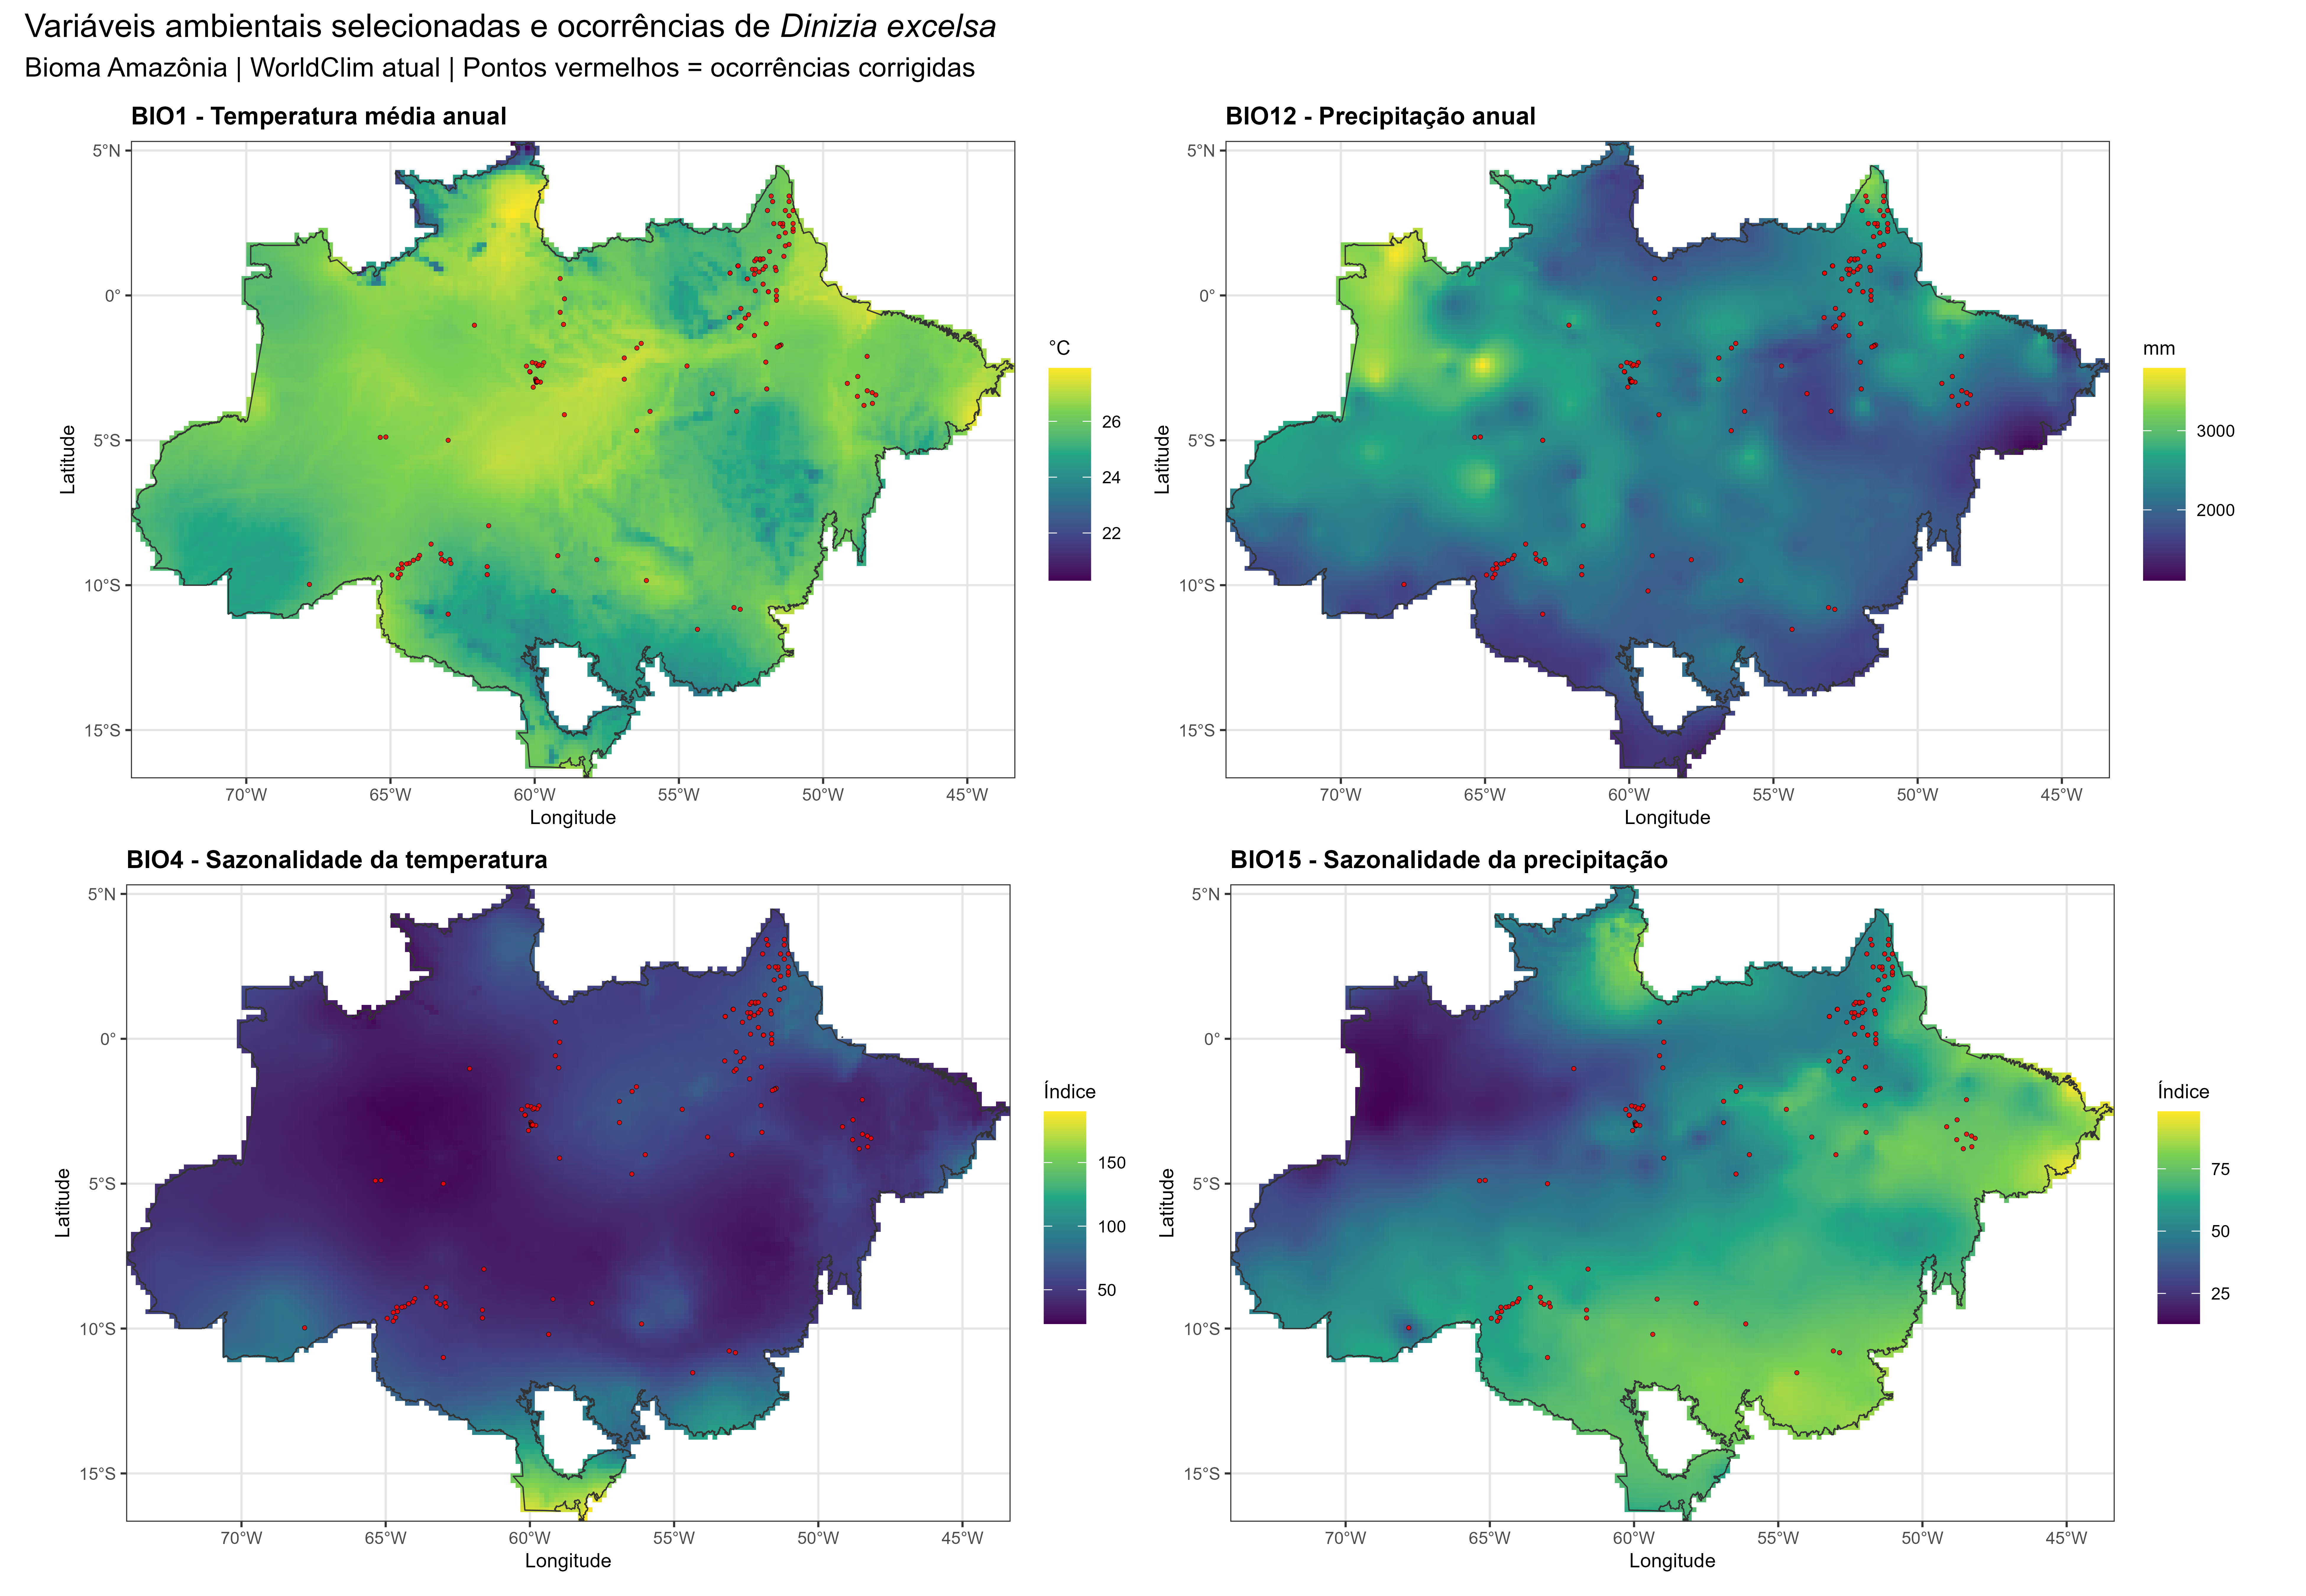
\includegraphics[width=0.96\textwidth]{figuras/unidade01/unidade01_mapas_variaveis_patchwork_dinizia.png}
  \caption{Selected environmental variables across the Amazon biome and corrected records of \textit{Dinizia excelsa}. Each panel uses an independent color scale to show mean annual temperature, temperature seasonality, annual precipitation, and precipitation seasonality.}
  \label{fig:unidade01_variaveis_patchwork_dinizia}
\end{figure}

\begin{figure}[H]
  \centering
  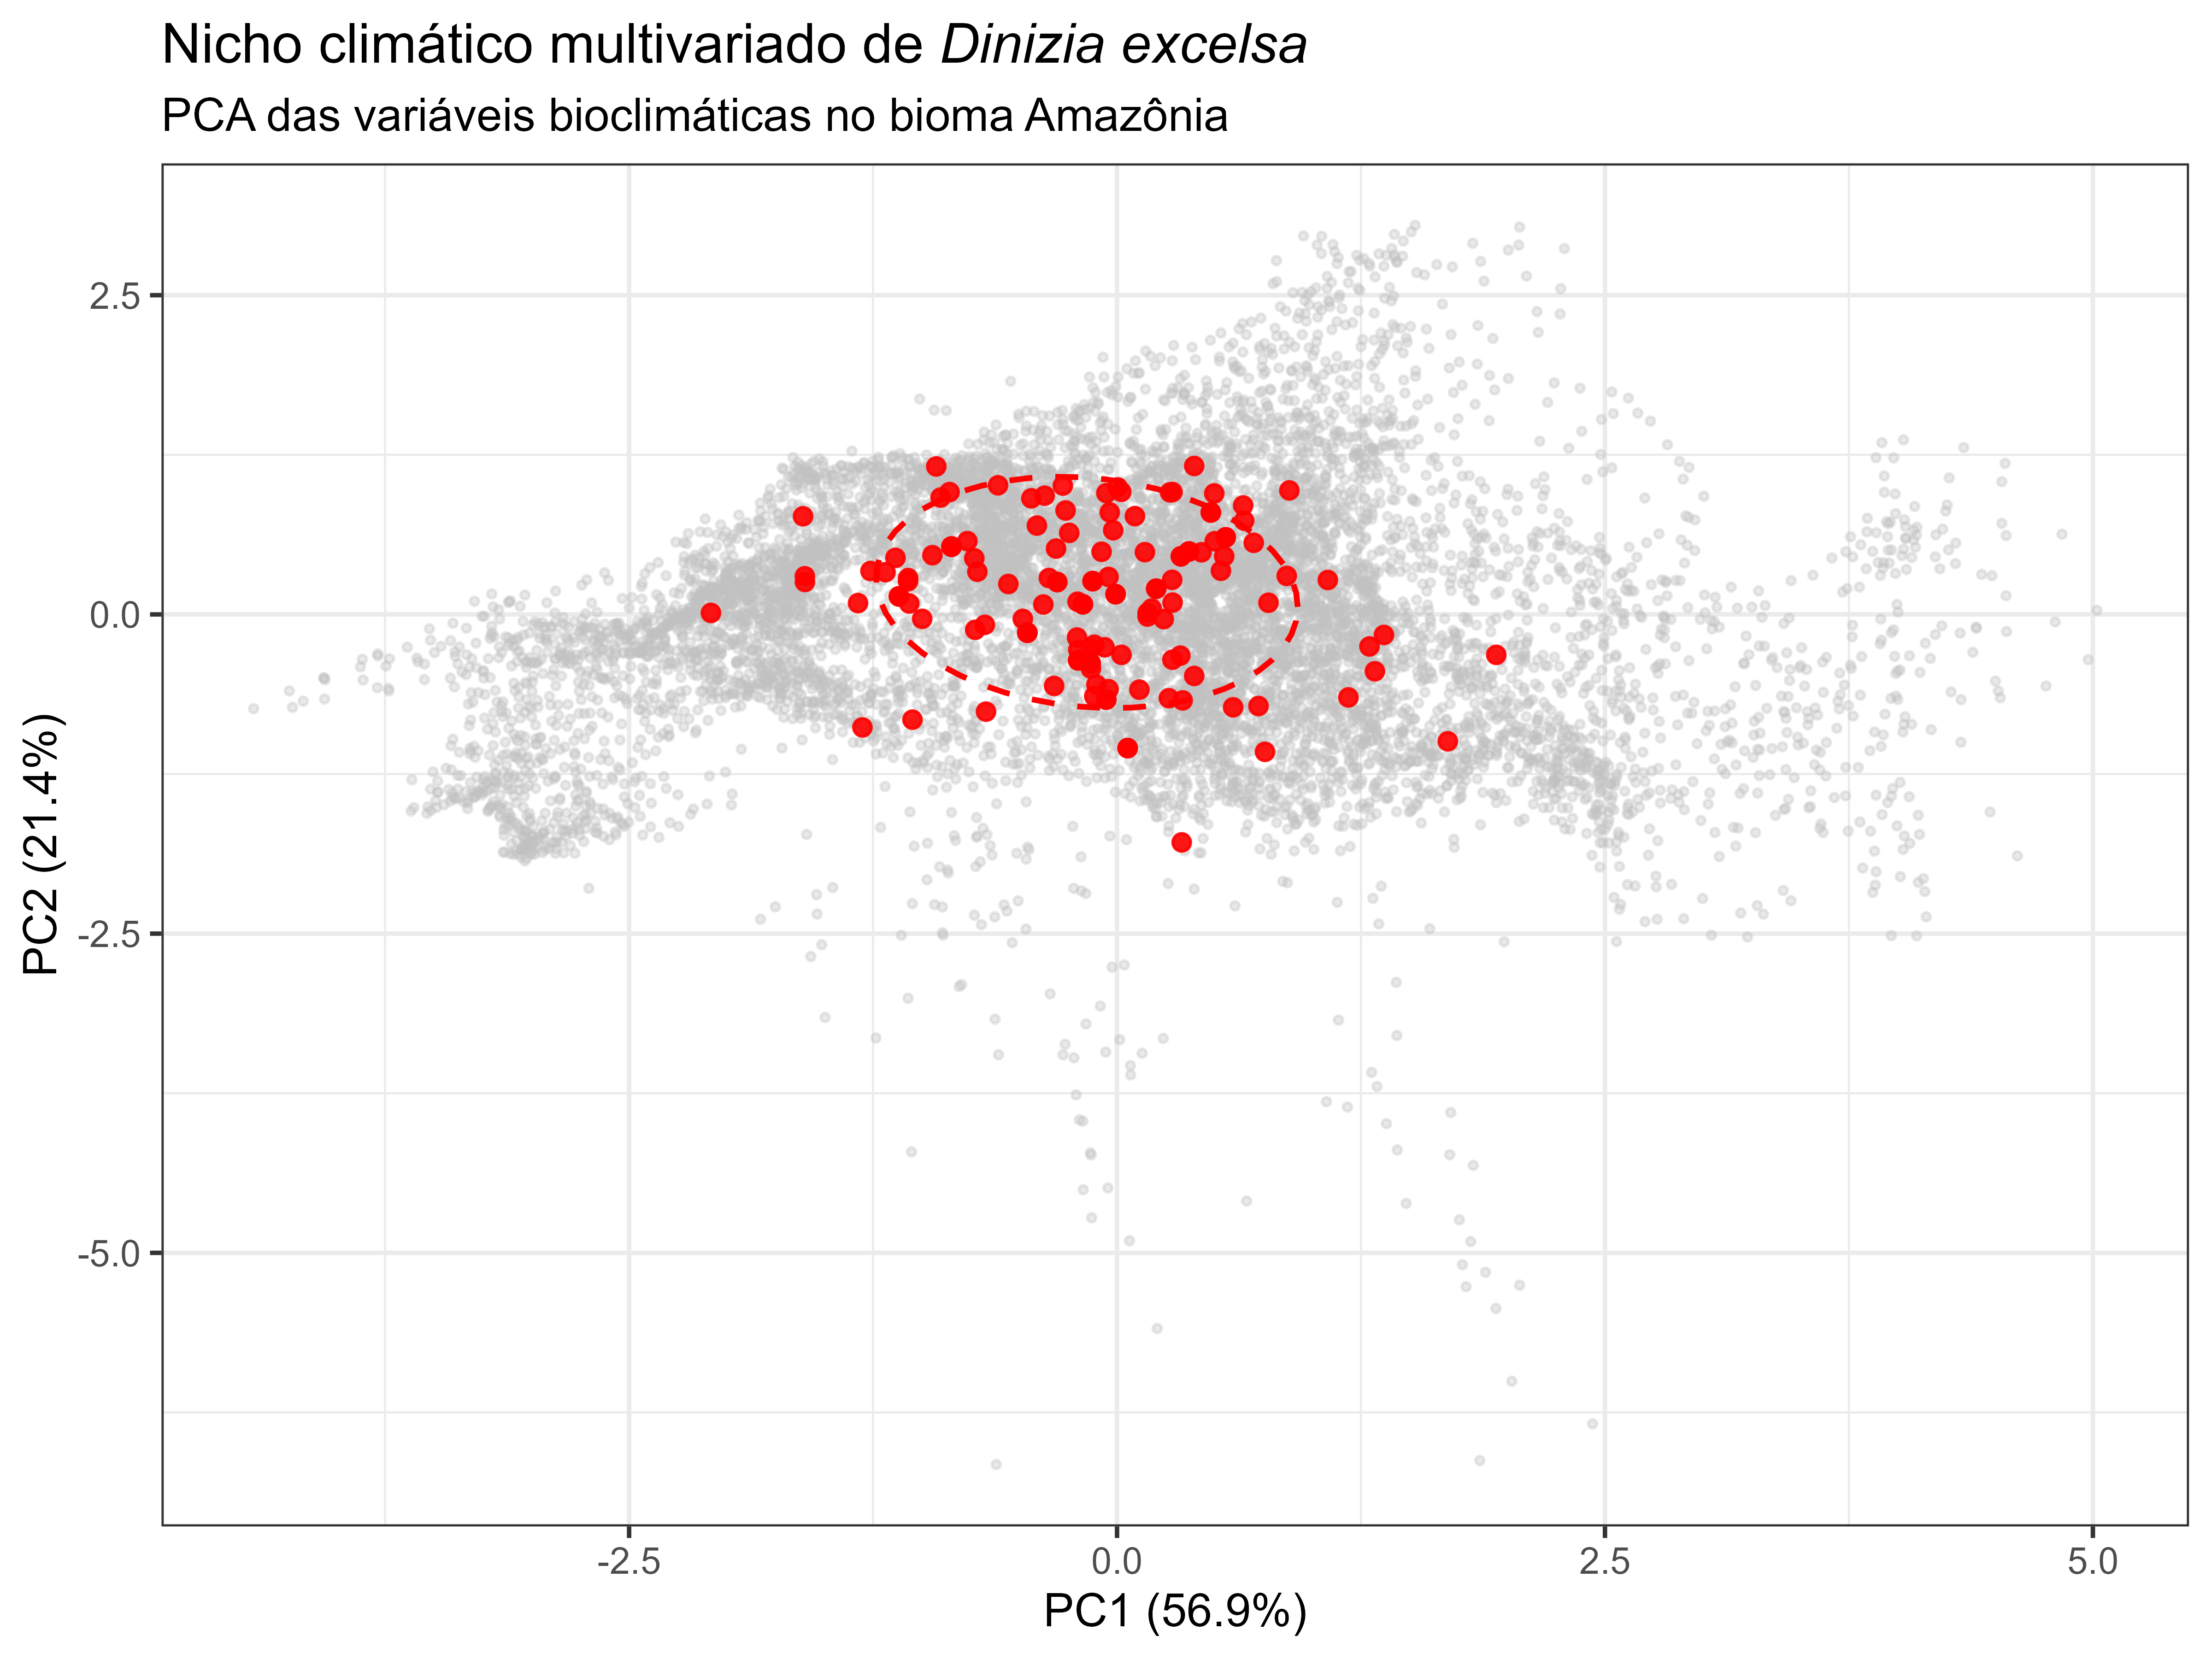
\includegraphics[width=0.82\textwidth]{figuras/unidade01/unidade01_pca_nicho_climatico_dinizia.png}
  \caption{Multivariate climatic niche of \textit{Dinizia excelsa}, represented by a PCA of the selected bioclimatic variables. Gray points represent the environmental background of the Amazon biome; red points are species occurrences.}
  \label{fig:unidade01_pca_dinizia}
\end{figure}

\begin{figure}[H]
  \centering
  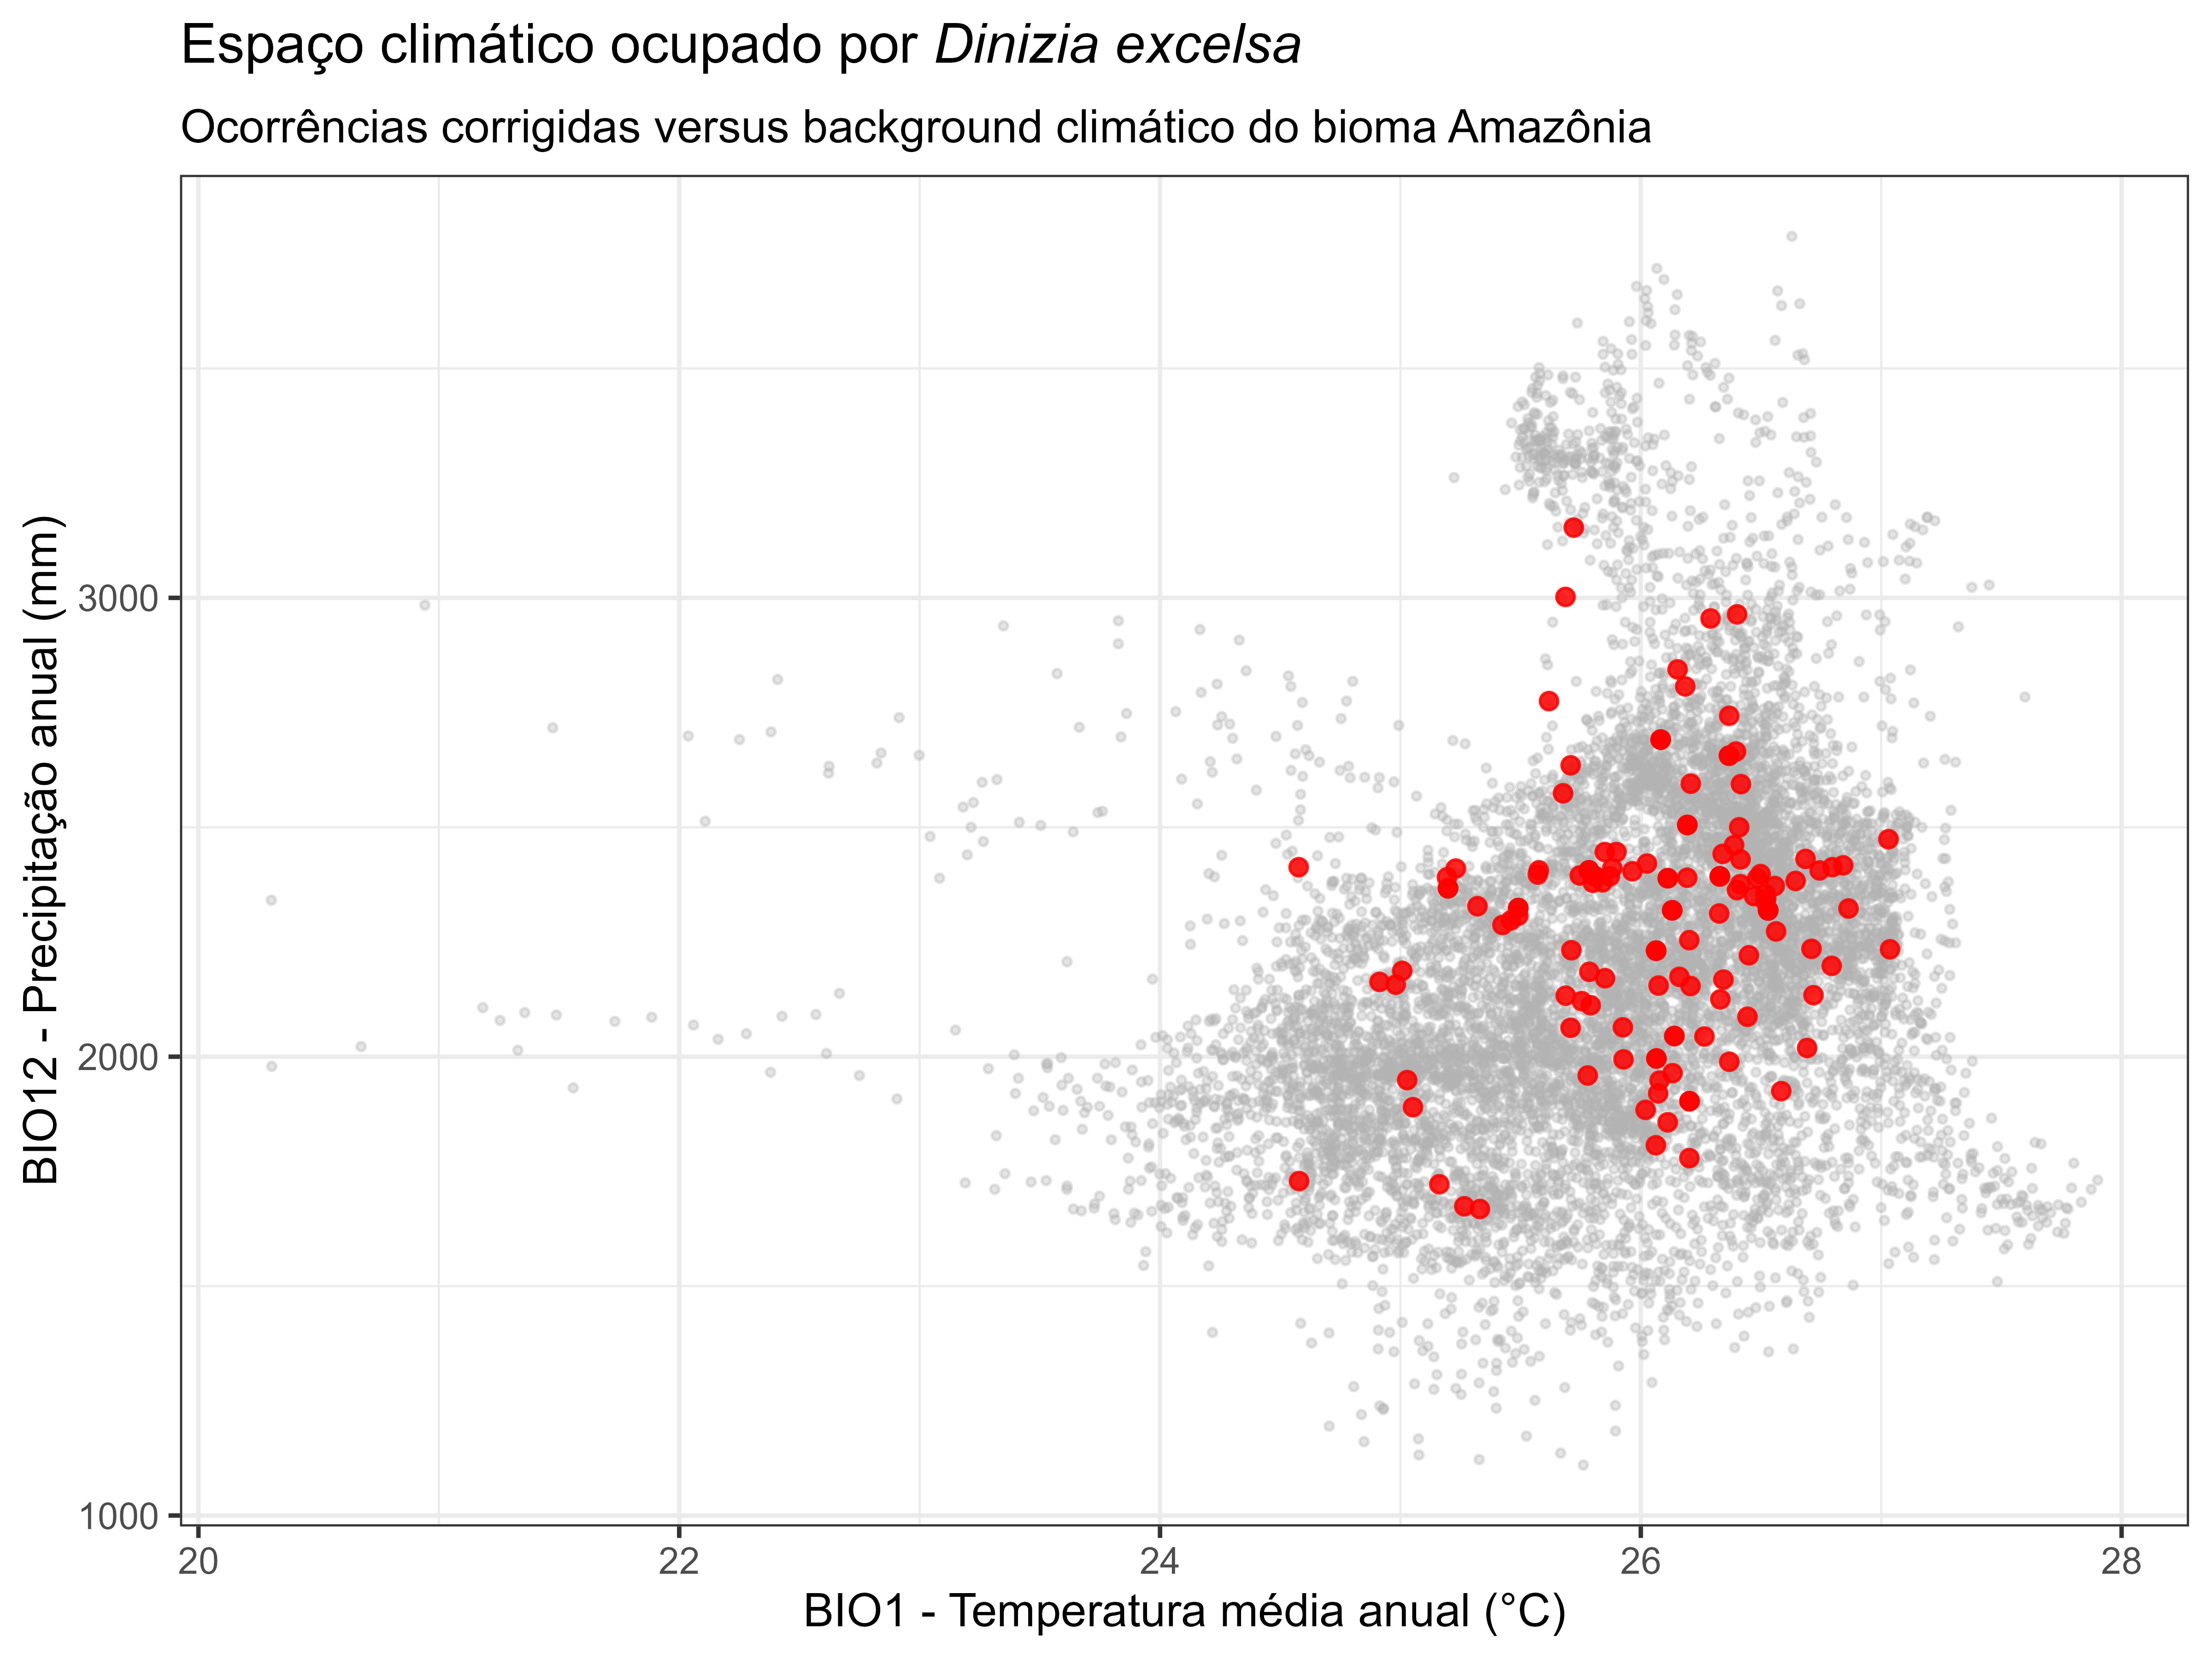
\includegraphics[width=0.82\textwidth]{figuras/unidade01/unidade01_nicho_temperatura_precipitacao_dinizia.png}
  \caption{Climatic space occupied by \textit{Dinizia excelsa} relative to the environmental background of the Amazon biome, based on mean annual temperature and annual precipitation.}
  \label{fig:unidade01_nicho_tp_dinizia}
\end{figure}

\begin{aplicacao}
Figures~\ref{fig:unidade01_pca_dinizia} and
\ref{fig:unidade01_nicho_tp_dinizia} show that the geographic distribution of
\textit{Dinizia excelsa} is associated with a specific subset of the climatic
conditions available across Amazonia. The bivariate plot shows occupation of
the climatic space defined by mean annual temperature and annual precipitation,
whereas the PCA represents the species in a multidimensional environmental
space. Occurrences are concentrated within a more restricted environmental
region than the full background, suggesting ecological filtering related to
the species' climatic requirements. In SDM, these relationships underpin niche
estimation and the projection of potentially suitable areas under present,
past, or future conditions.
\end{aplicacao}

\begin{exercicios}
\begin{enumerate}
  \item Explain the differences among the Grinnellian, Eltonian, and Hutchinsonian niches.
  \item Why do occurrence-based distribution models generally approximate the realized niche rather than the fundamental niche?
  \item Distinguish observed, actual, and potential distributions.
  \item Why should the absence of a biodiversity record not automatically be interpreted as ecological absence?
  \item Discuss the importance of niche conservatism for future climate projections.
  \item For large Amazonian tree species, which factors might cause the distribution of adults to misrepresent the potential distribution of recruits?
\end{enumerate}
\end{exercicios}

\chapter[Occurrence Data]{Occurrence Data, Spatial Cleaning, and Record Preparation}

\begin{objetivos}
By the end of this chapter, readers should be able to identify the main sources
of occurrence data used in species distribution modeling; recognize limitations
of herbarium, inventory, and global-repository data; standardize taxonomic and
geographic records; filter occurrences using the Amazon biome boundary; remove
problematic coordinates, duplicates, and spatially redundant records; apply
spatial thinning; extract environmental values at occurrence locations; and
prepare a final occurrence dataset for subsequent modeling chapters.
\end{objetivos}

\section{Introduction}

Occurrence data provide the empirical foundation of species distribution
modeling. In correlative models, geographic records are associated with the
environmental conditions at locations where a species was observed, making it
possible to estimate occurrence--environment relationships. Model quality,
however, depends directly on the quality of these records.

In real applications, occurrence data may originate from forest inventories,
herbaria, biological collections, digital platforms, scientific literature,
and global repositories such as GBIF. These sources frequently combine
different levels of taxonomic, geographic, and temporal precision. Careful
standardization, cleaning, and spatial filtering are therefore required before
model fitting \parencite{guisan2017habitat,hijmans2021species,zizka2019coordinatecleaner}.

\begin{conceito}[title={\faBook\quad Occurrence record}]
An occurrence record is spatial evidence that a species was present at a given
location. In SDM, it is usually represented by geographic coordinates linked to
the species name, data source, and, when available, date, institution,
collector, and spatial uncertainty.
\end{conceito}

\section{Sources of Occurrence Data}

SDM data can come from several sources. Forest inventories generally provide
stronger taxonomic and spatial control but tend to cover limited areas.
Herbaria and biological collections contain valuable historical records,
although coordinates may be missing or imprecise. Global platforms such as
GBIF increase spatial coverage but require stringent quality filters.

In the reference study used throughout this textbook, records of
\textit{Dinizia excelsa} from inventories and GBIF were integrated and then
subjected to spatial filters, thinning, and extraction of bioclimatic variables
for climatic-niche analysis across Amazonia \parencite{delima2026warmer}. This
chapter implements a comparable workflow.

\begin{dica}[title={\faLightbulb\quad Integrating sources}]
A robust occurrence dataset may combine inventories, herbaria, and GBIF,
provided that every record undergoes standardization, cleaning, and duplicate
control.
\end{dica}

\section{Common Problems in Occurrence Data}

Frequent problems include inconsistent scientific names, invalid coordinates,
marine records for terrestrial species, points located at national or regional
capitals, institutional coordinates, duplicates, reversed latitude and
longitude, georeferencing errors, and strong spatial sampling bias.

For Amazonian species, records are often concentrated near rivers, roads,
cities, herbaria, forest-inventory sites, and logistically accessible regions.
Such patterns do not necessarily indicate greater environmental suitability;
they may instead reflect greater collection effort.

\begin{atencao}[title={\faExclamationTriangle\quad Lack of occurrence is not absence}]
Presence records indicate where a species was observed. A region without
records does not necessarily lack the species; it may simply have received
little or no sampling effort.
\end{atencao}

\section{Data-Preparation Workflow}

The workflow follows the general structure of Amazon-scale SDM studies:
compile records, standardize columns, retain valid coordinates, apply geographic
quality control, crop to the biome, remove duplicates, perform spatial thinning,
extract environmental data, and export the final dataset.

\rscriptfile{scripts/unidade02/01_compilar_ocorrencias_dinizia.R}

\section{Geographic Cleaning and Cropping to the Amazon Biome}

After compilation, records are converted to spatial objects, checked for
coordinate validity, and filtered using the Amazon biome boundary. This step
ensures that the working dataset represents the geographic extent defined for
the study.

\rscriptfile{scripts/unidade02/02_limpeza_espacial_dinizia.R}

\begin{figure}[H]
  \centering
  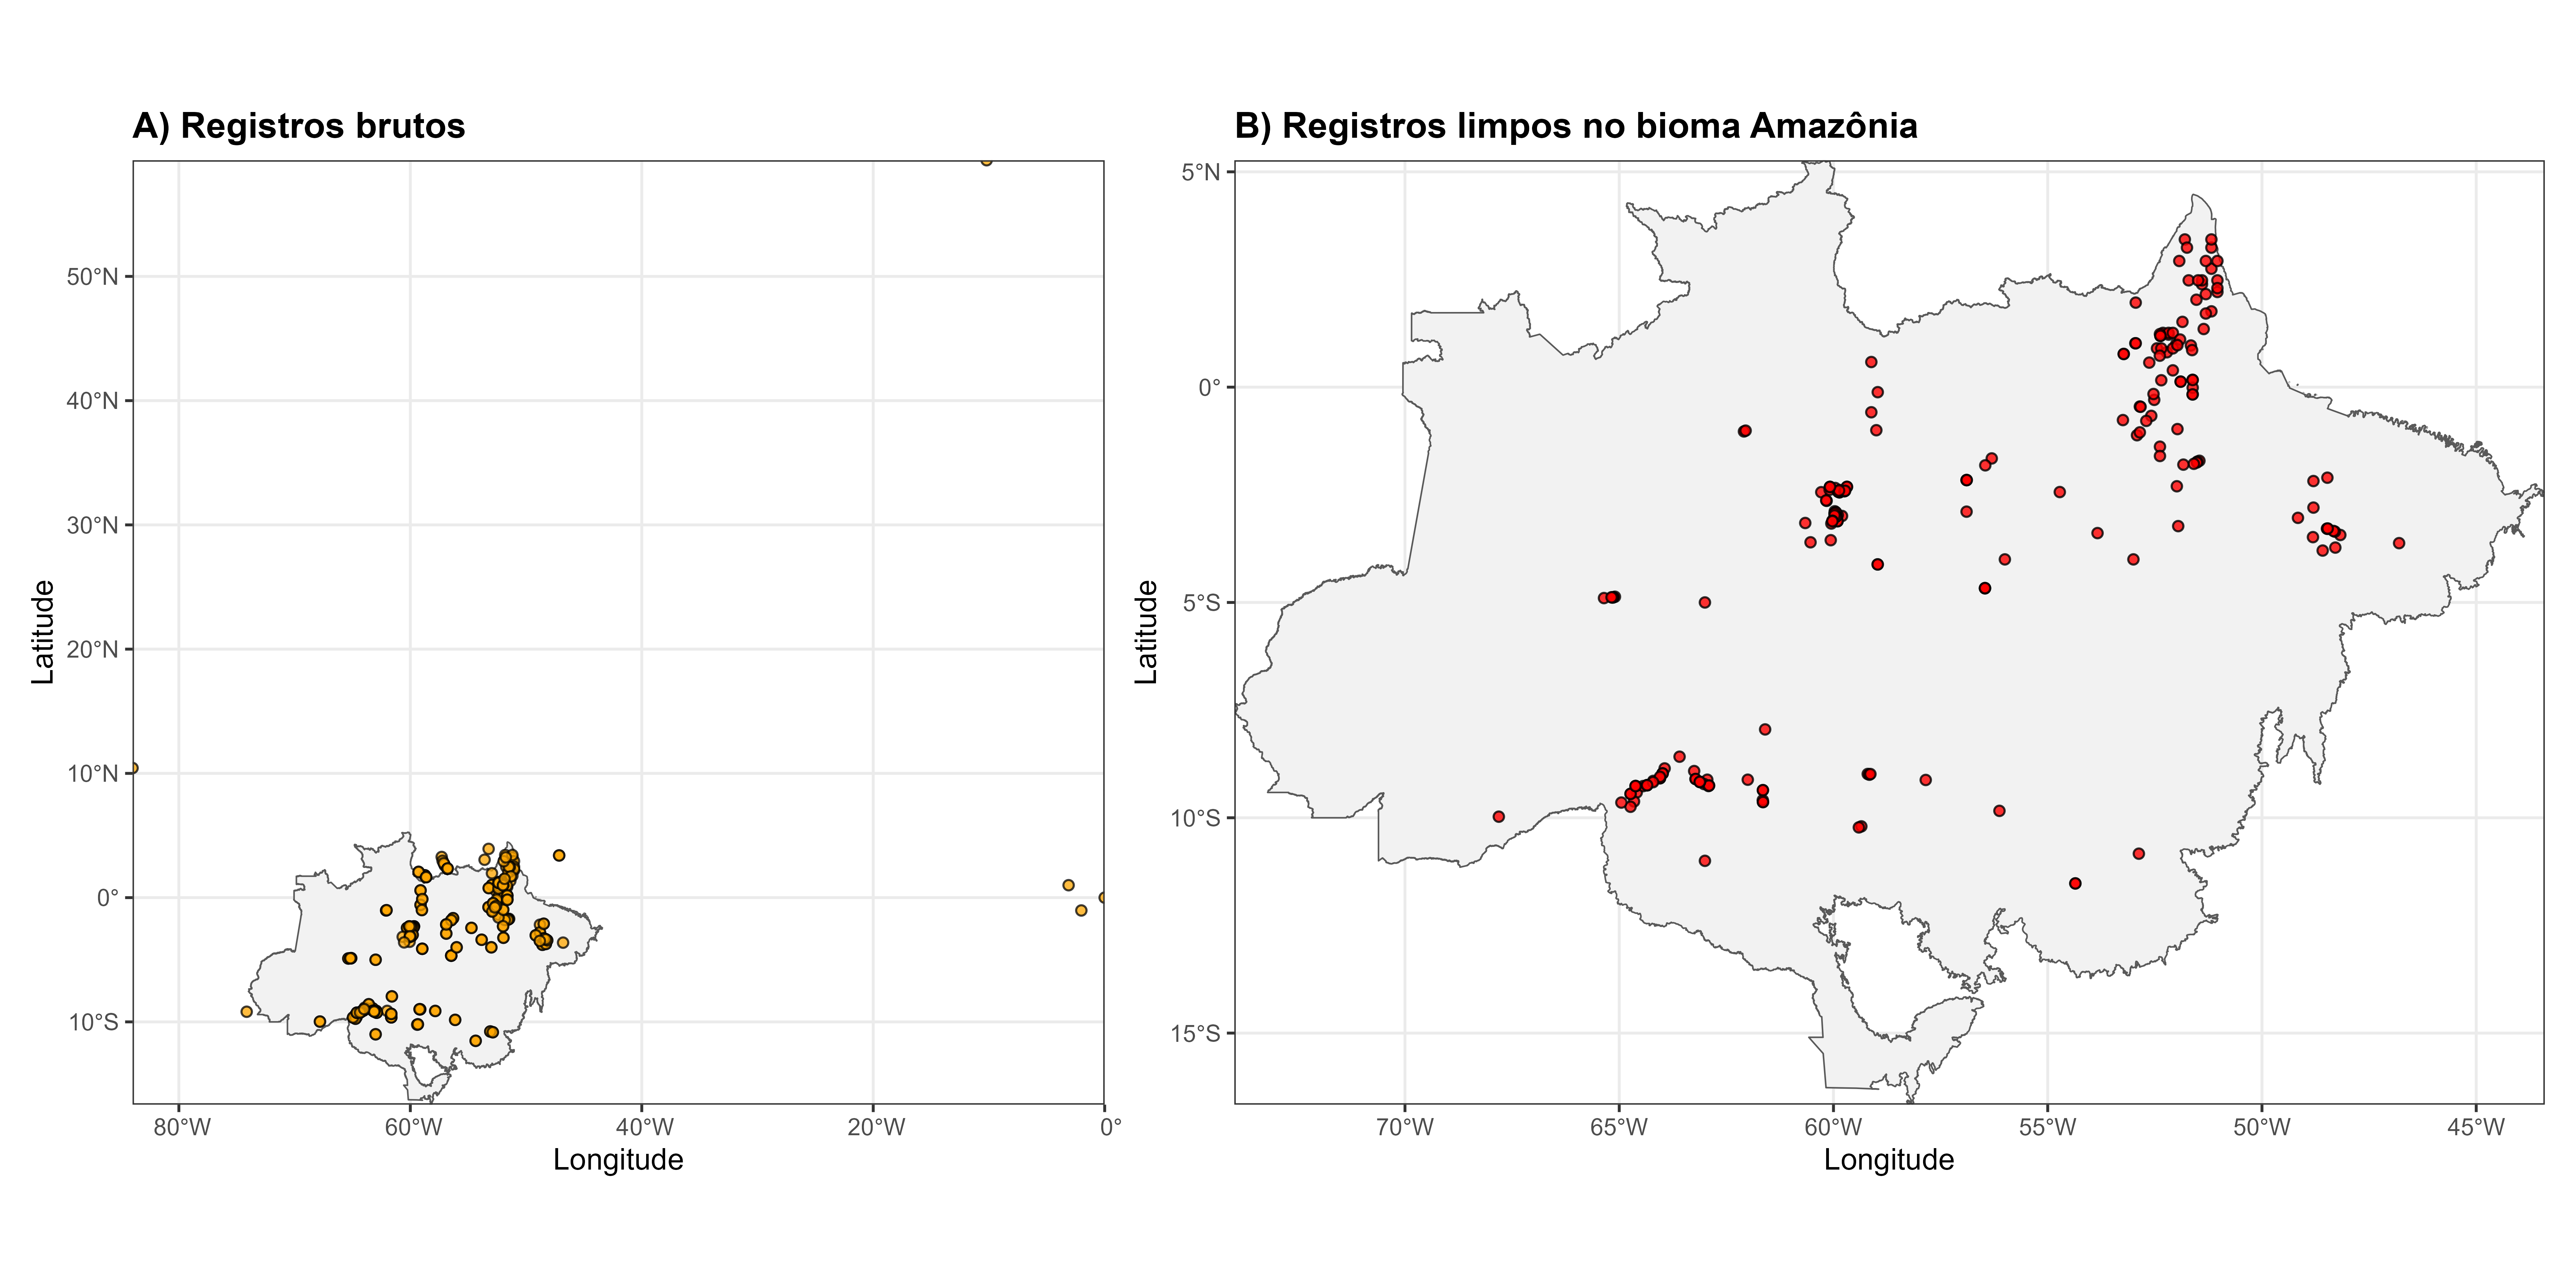
\includegraphics[width=0.92\textwidth]{figuras/unidade02/unidade02_mapa_bruto_limpo_dinizia.png}
  \caption{Comparison of raw and filtered records of \textit{Dinizia excelsa} within the Amazon biome.}
  \label{fig:unidade02_bruto_limpo_dinizia}
\end{figure}

\section{Environmental Extraction and Raster-Cell Duplicates}

Even after identical coordinates have been removed, different records may fall
within the same climatic raster cell. Because models use environmental values
extracted from rasters, multiple points in one cell may constitute environmental
pseudoreplication. It is therefore advisable to retain only one occurrence per
environmental raster cell.

\rscriptfile{scripts/unidade02/03_extrair_ambiente_dinizia.R}

\section{Spatial Thinning}

Spatial thinning reduces excessive concentrations of records in intensively
sampled areas. Here, a minimum distance is imposed between retained
occurrences, helping to reduce spatial autocorrelation and sampling bias. This
procedure is widely used in ecological-niche studies and can be implemented
with the \texttt{spThin} package \parencite{aiellolammens2015spthin}.

\rscriptfile{scripts/unidade02/04_rarefacao_espacial_dinizia.R}

\begin{figure}[H]
  \centering
  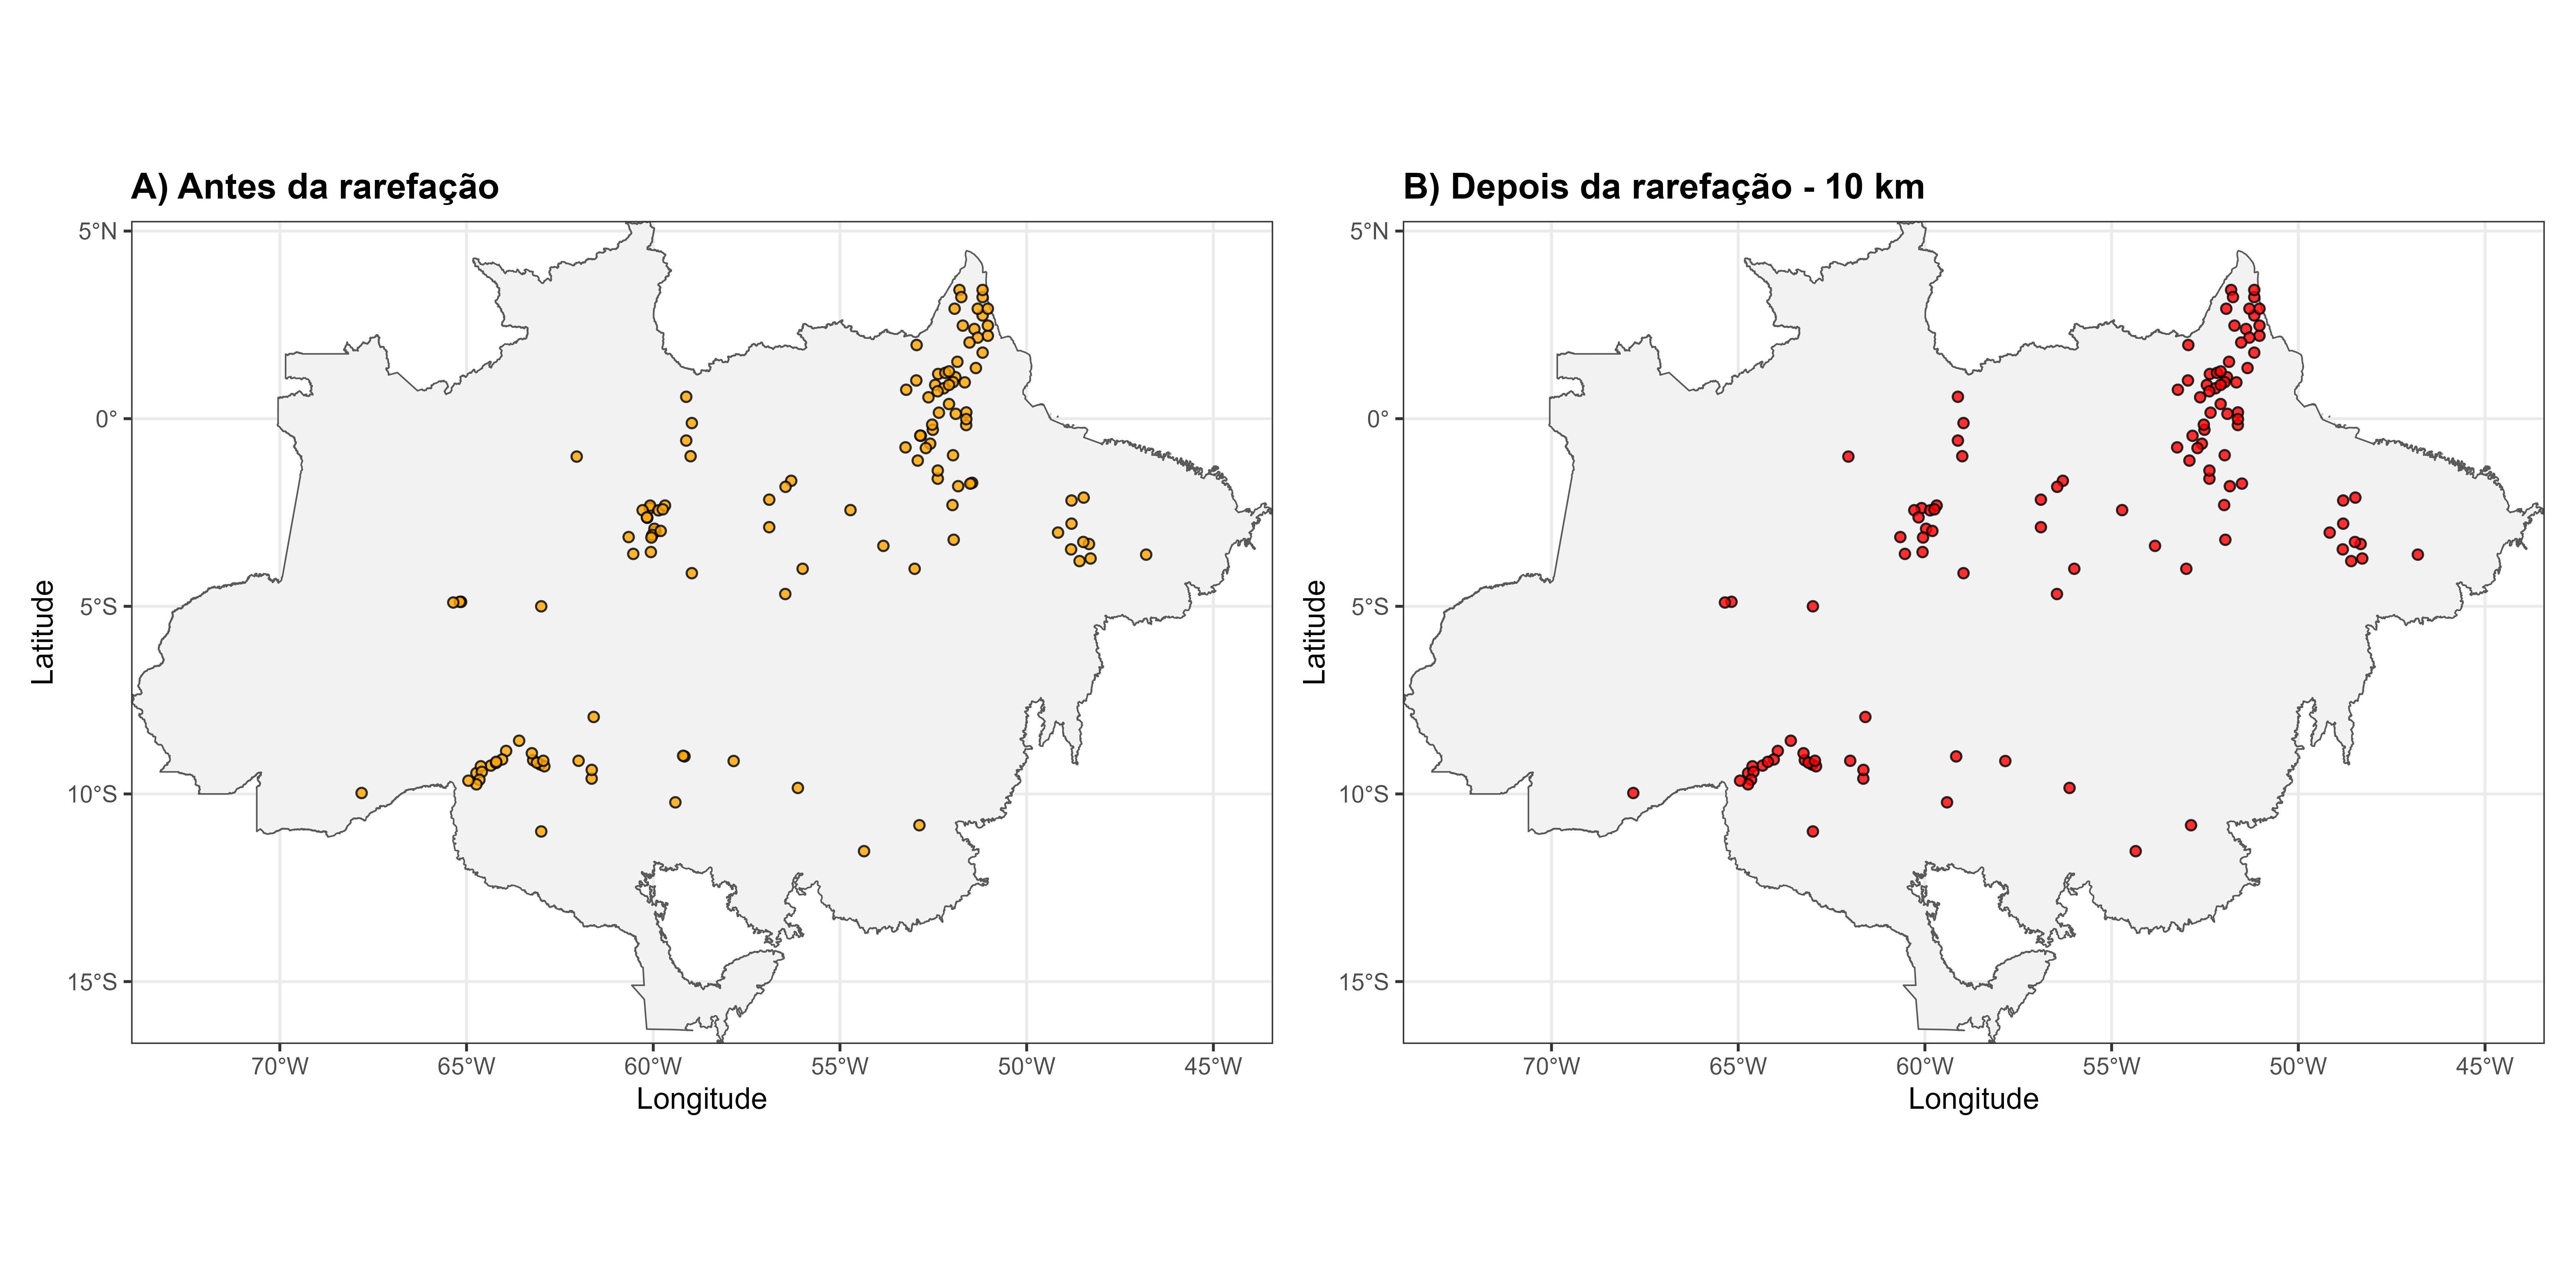
\includegraphics[width=0.92\textwidth]{figuras/unidade02/unidade02_rarefacao_dinizia.png}
  \caption{Effect of spatial thinning on records of \textit{Dinizia excelsa}. The procedure reduces spatial redundancy and concentrations of nearby points.}
  \label{fig:unidade02_rarefacao_dinizia}
\end{figure}

\section{Environmental Diagnostics of the Records}

After cleaning and thinning, the final occurrences are associated with the
selected environmental variables. This step characterizes the climatic range
occupied by the species, identifies extreme values, and prepares the final
matrix for model fitting.

\rscriptfile{scripts/unidade02/05_diagnostico_ambiental_dinizia.R}

\begin{figure}[H]
  \centering
  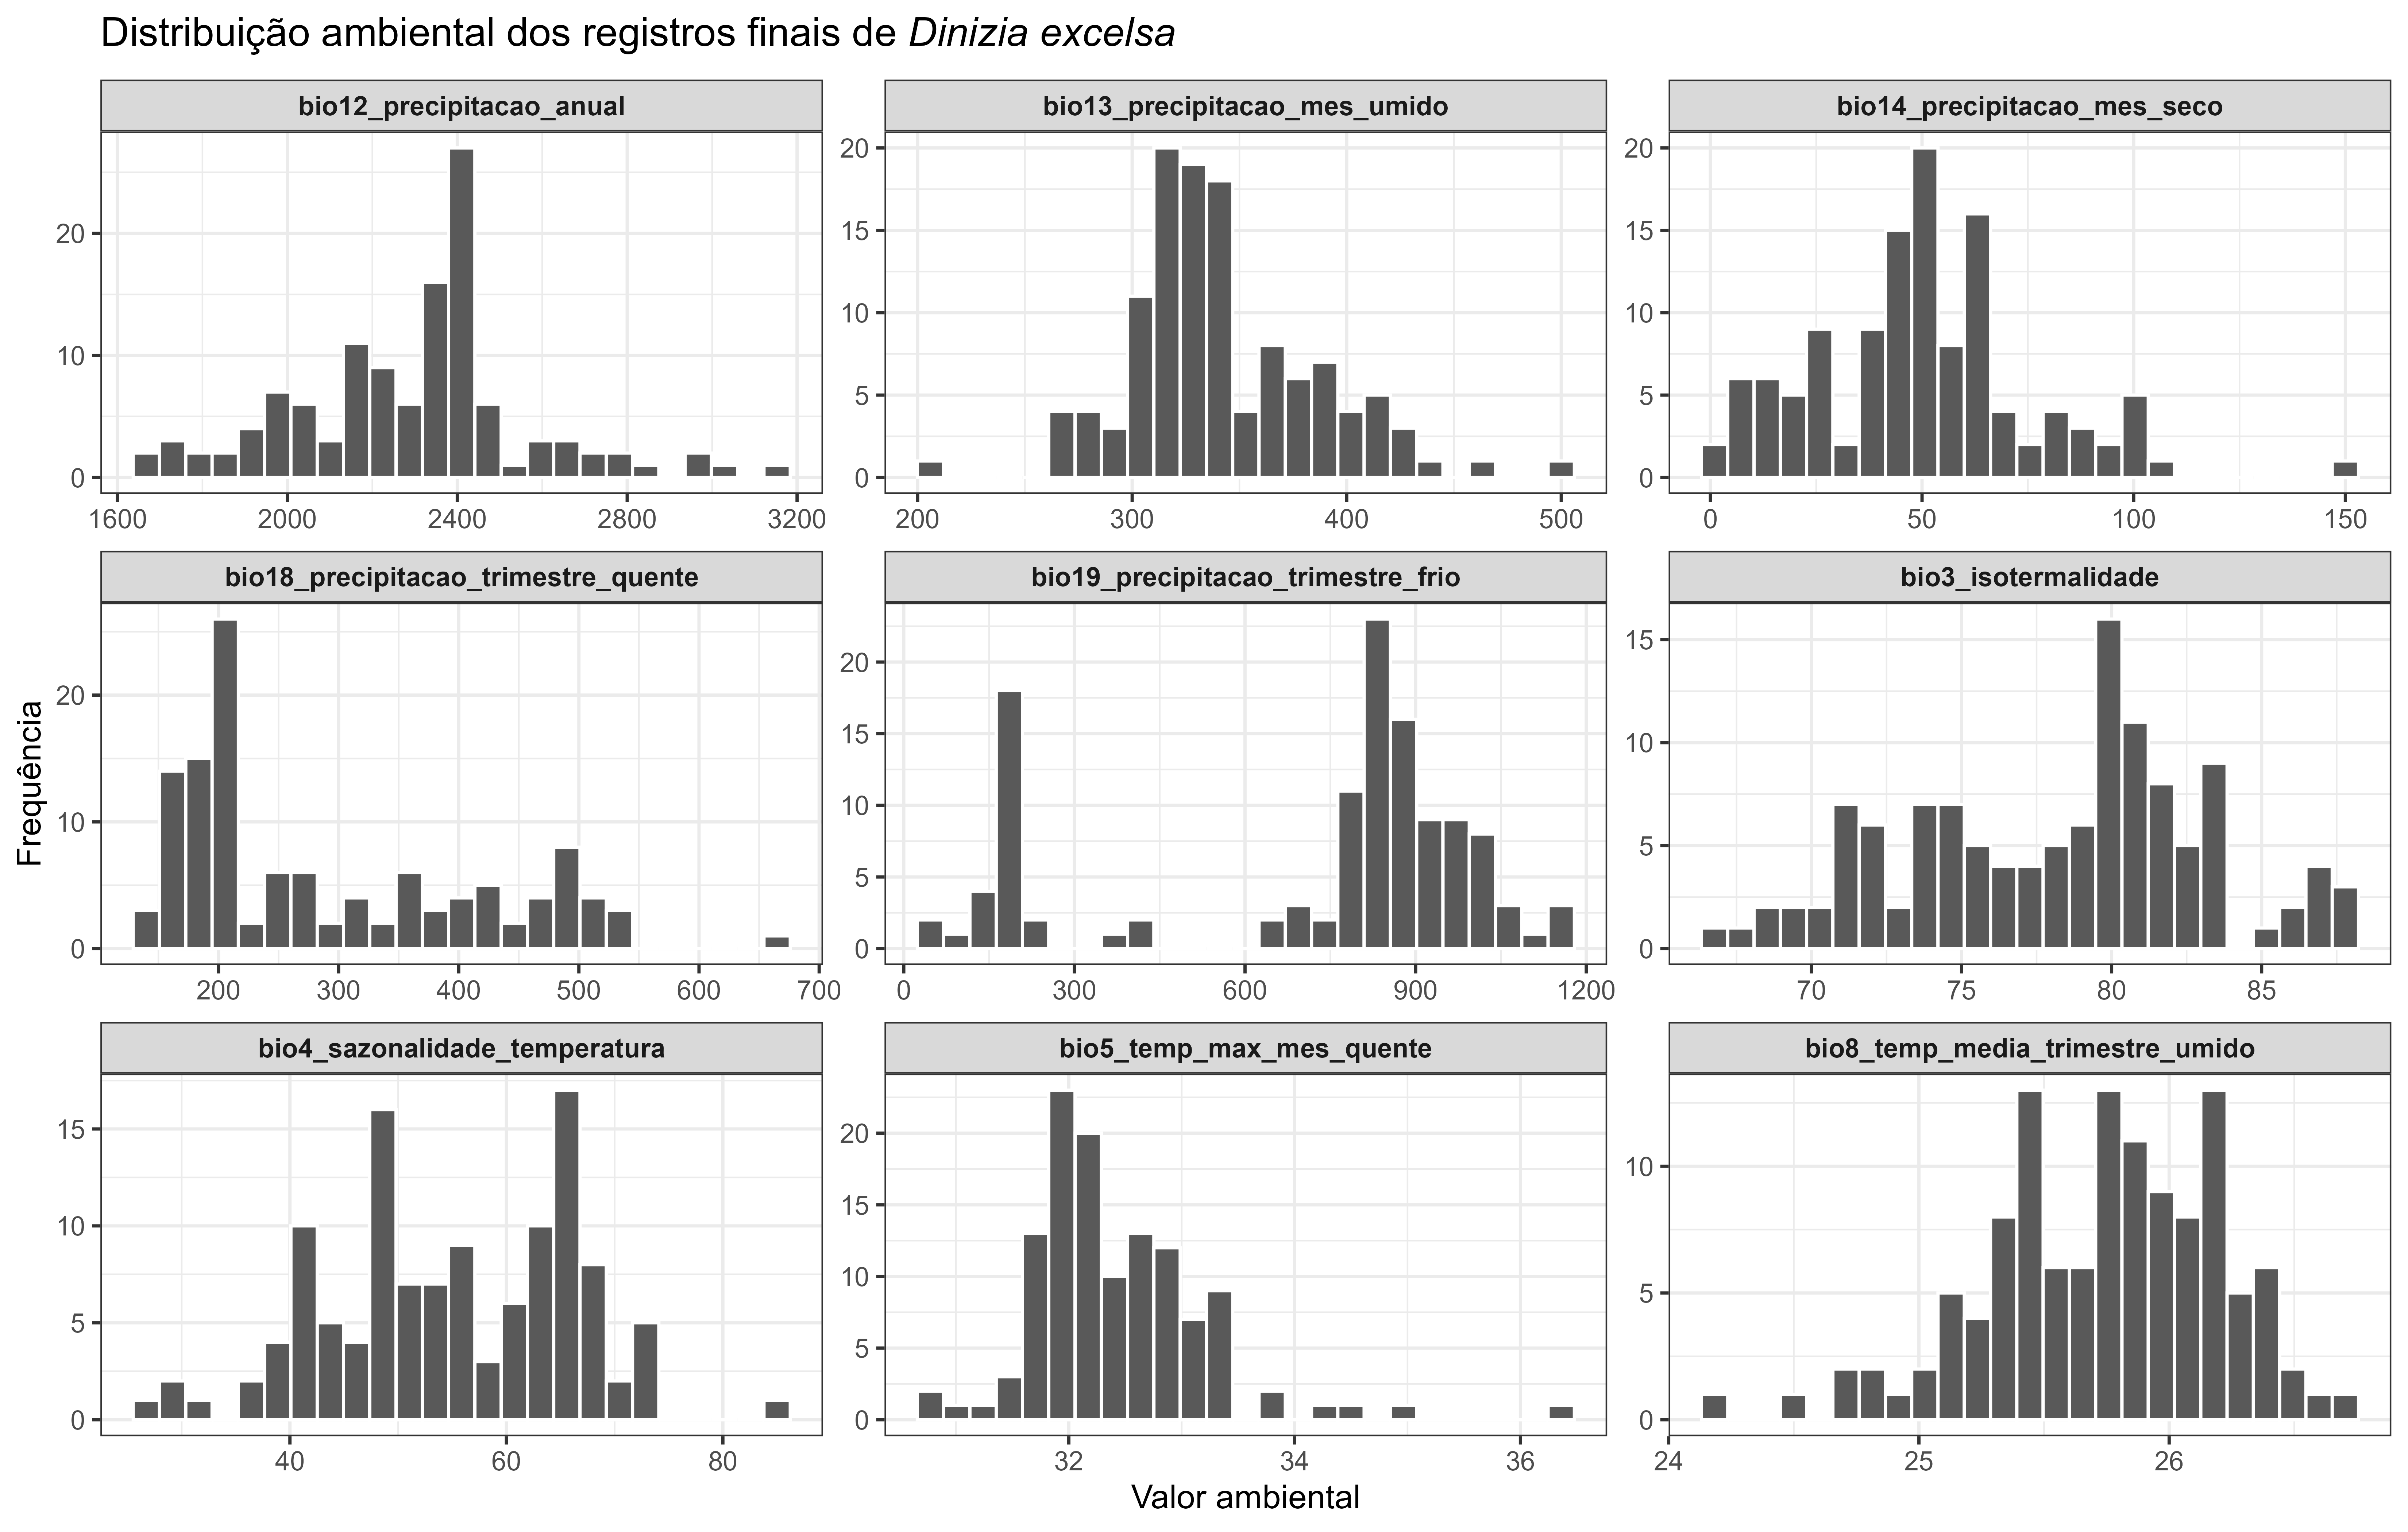
\includegraphics[width=0.92\textwidth]{figuras/unidade02/unidade02_histogramas_variaveis_dinizia.png}
  \caption{Distributions of bioclimatic variables extracted at the final \textit{Dinizia excelsa} occurrence locations.}
  \label{fig:unidade02_hist_variaveis_dinizia}
\end{figure}

\begin{figure}[H]
  \centering
  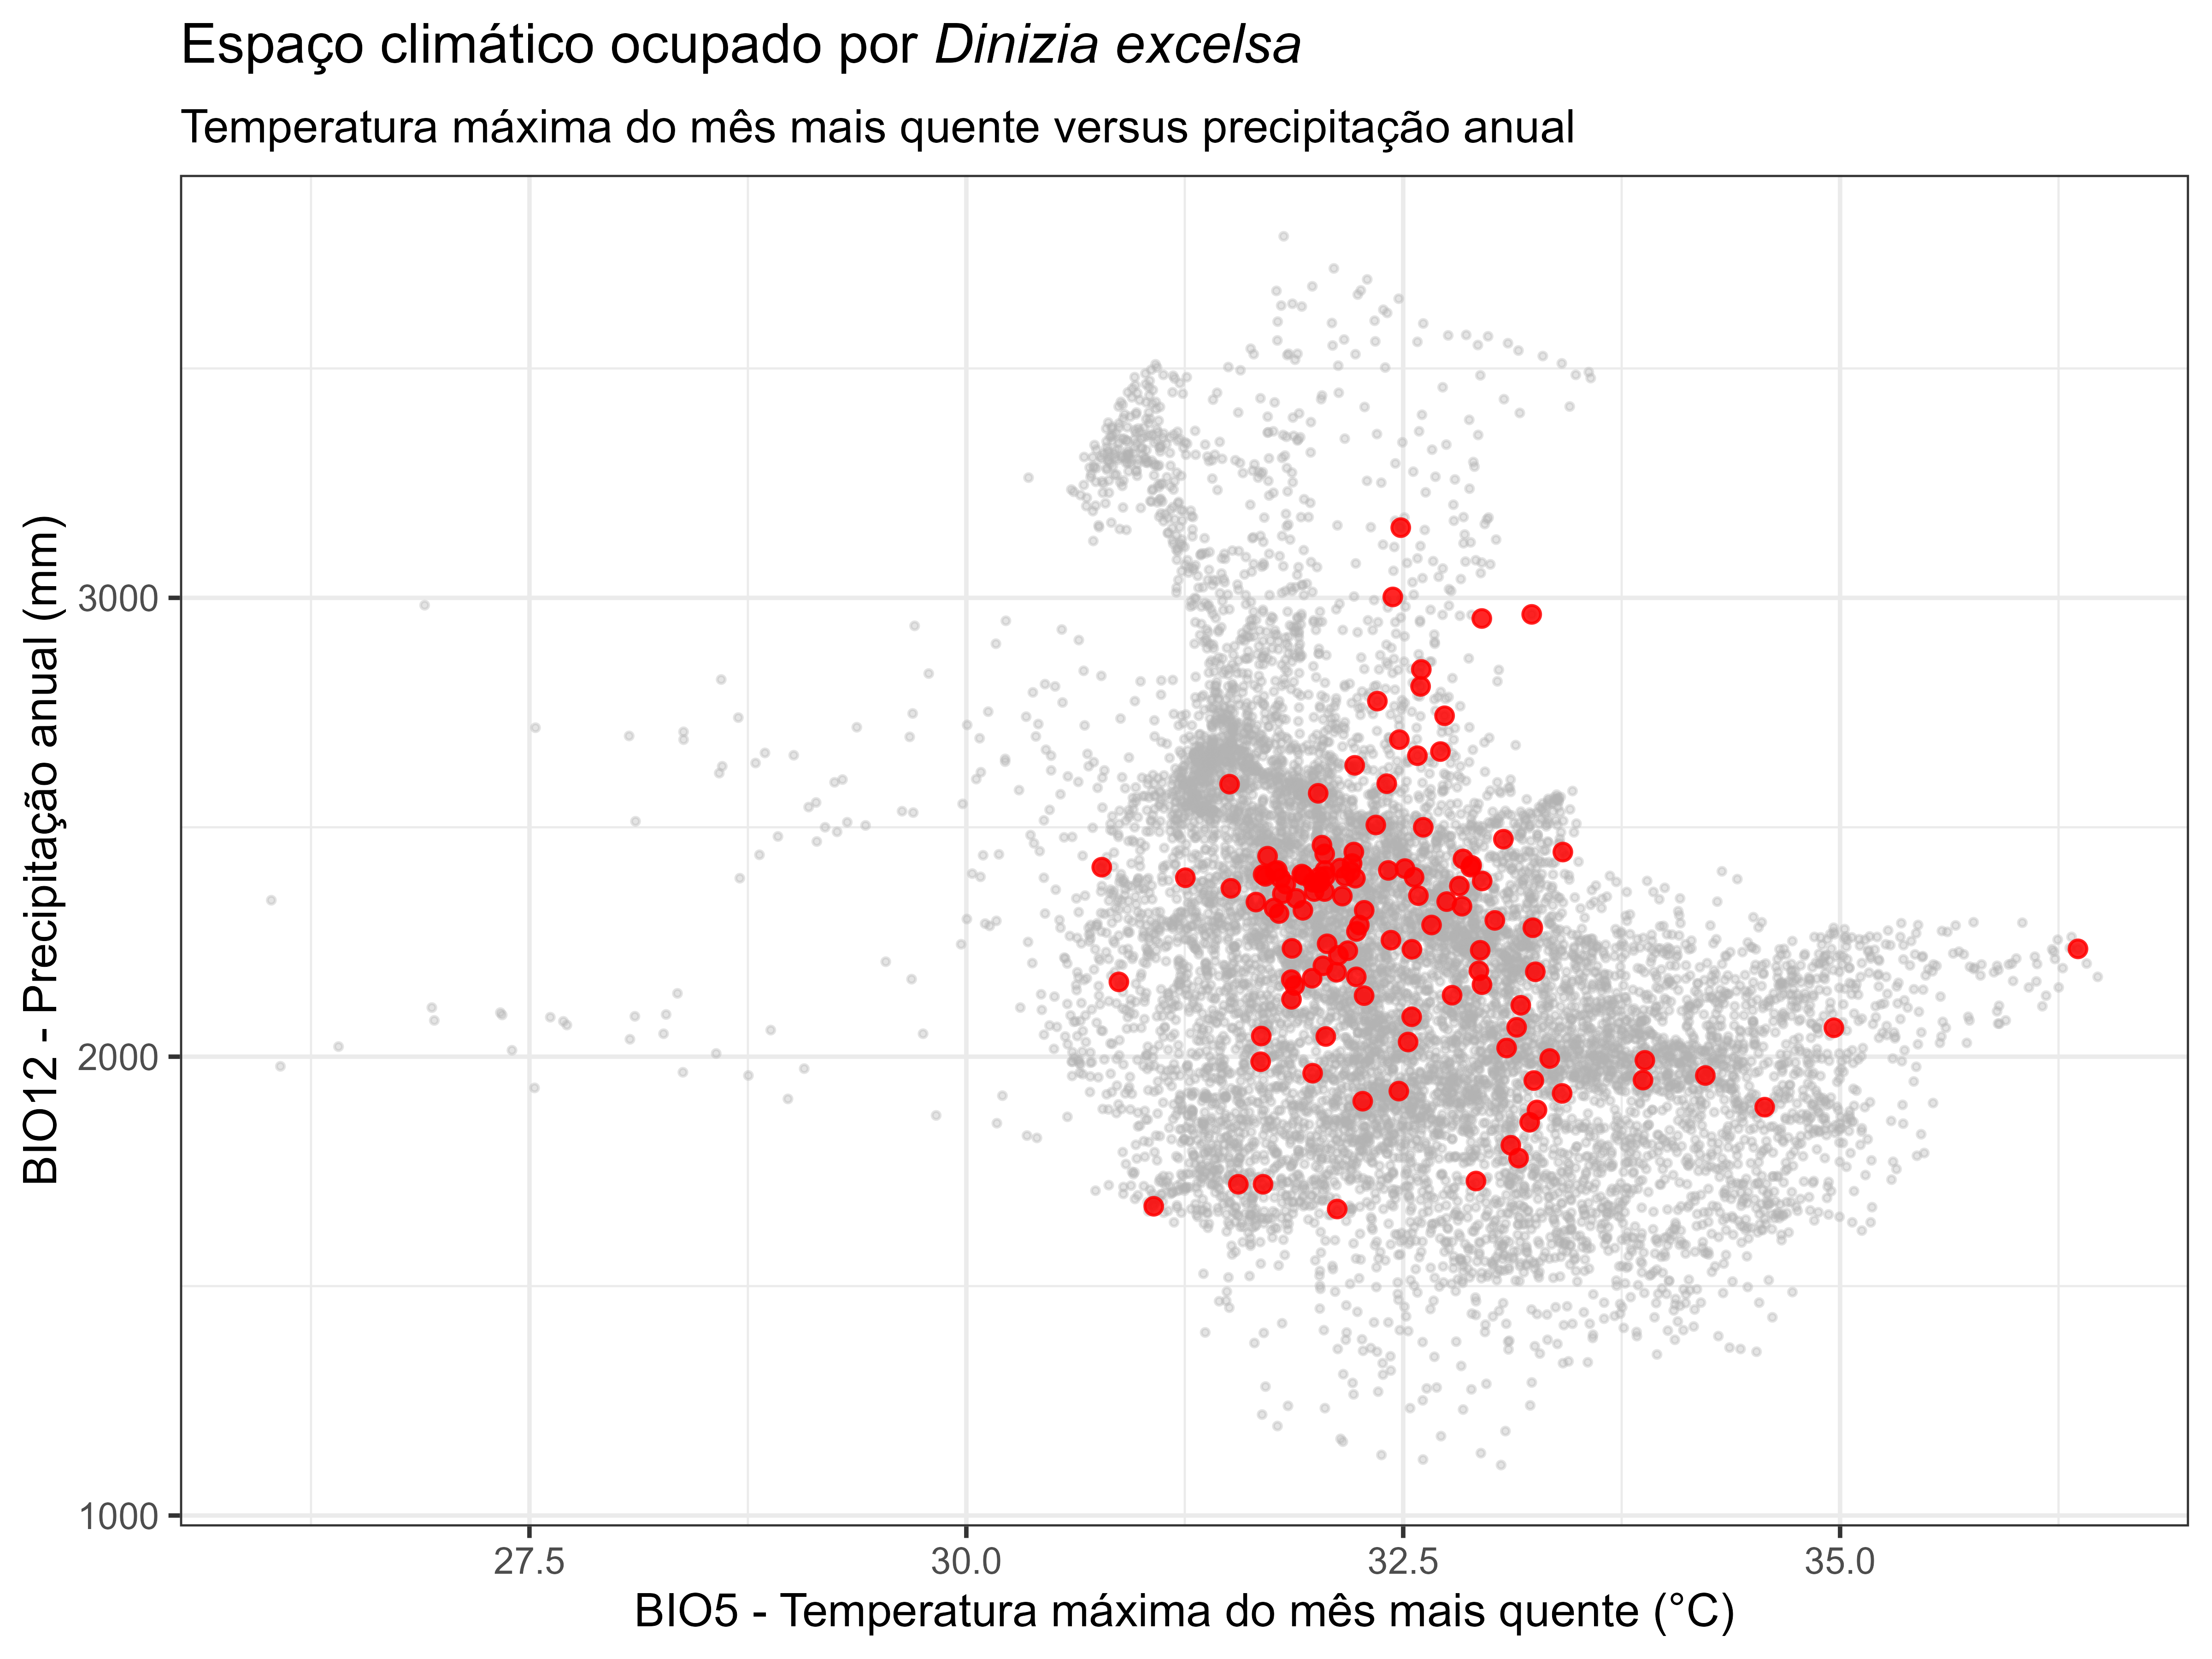
\includegraphics[width=0.86\textwidth]{figuras/unidade02/unidade02_espaco_climatico_dinizia.png}
  \caption{Climatic space occupied by \textit{Dinizia excelsa} relative to the environmental background of the Amazon biome.}
  \label{fig:unidade02_espaco_climatico_dinizia}
\end{figure}

\section{Processing Flowchart}

The flowchart summarizes the decisions used to transform raw occurrence
records into a modeling-ready dataset.

\rscriptfile{scripts/unidade02/06_fluxograma_preparacao_dinizia.R}

\begin{figure}[H]
  \centering
  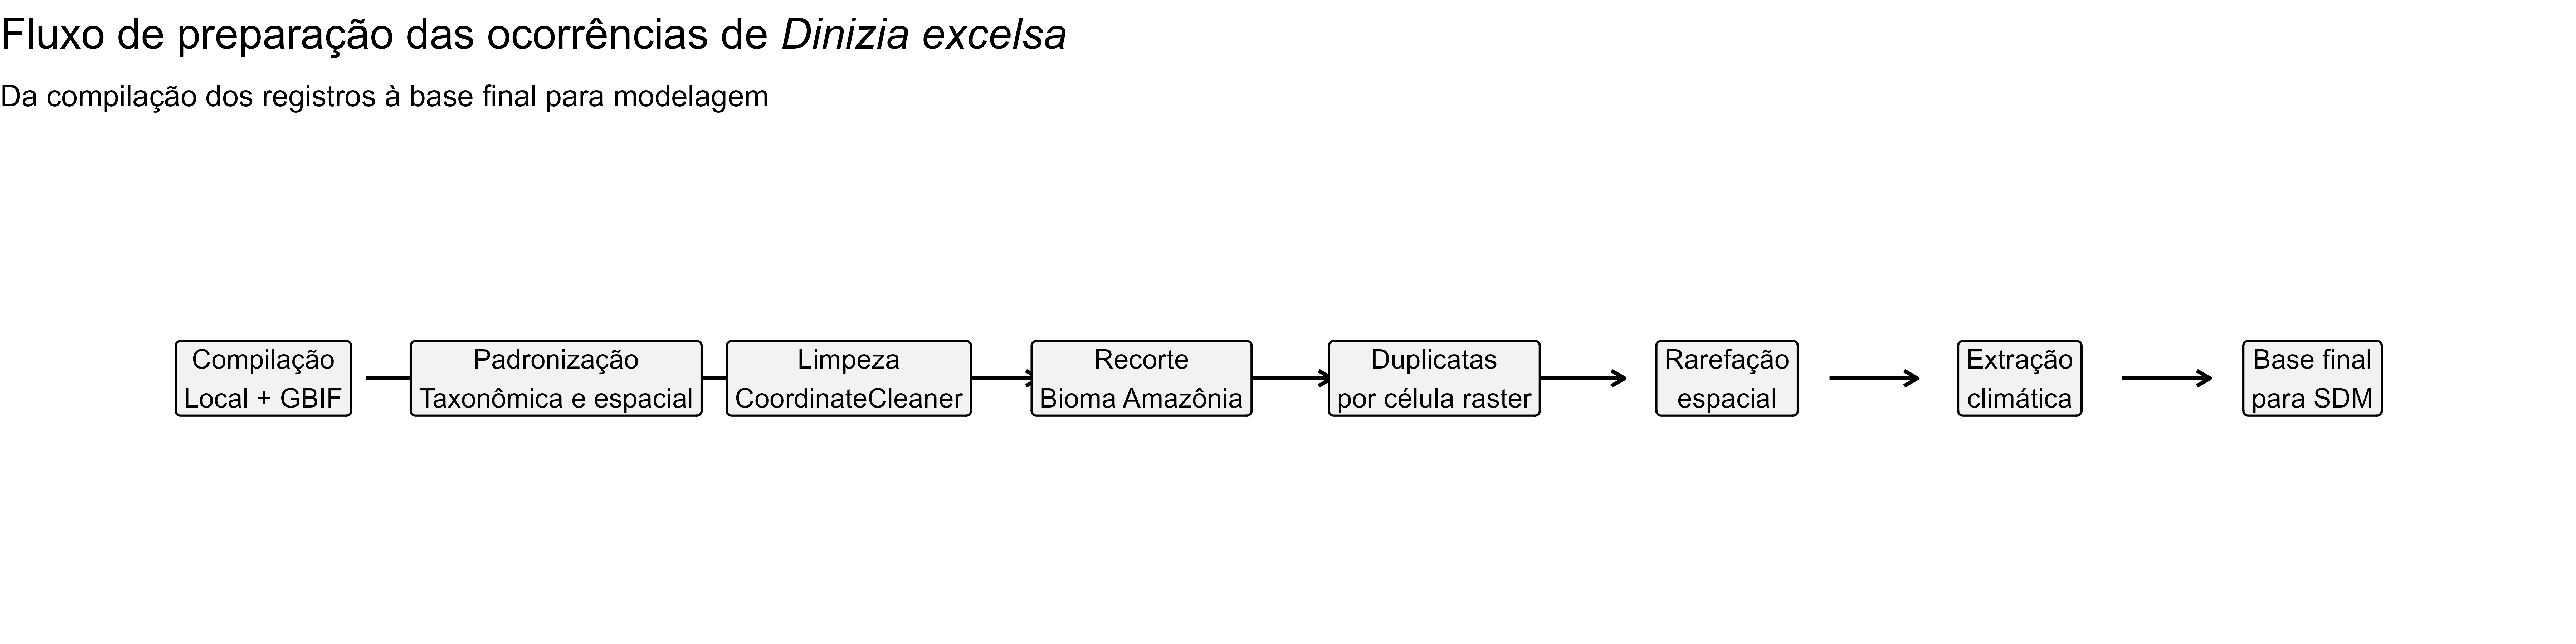
\includegraphics[width=0.92\textwidth]{figuras/unidade02/unidade02_fluxograma_preparacao_dinizia.png}
  \caption{Occurrence-data preparation workflow for SDM, using \textit{Dinizia excelsa} as a case study.}
  \label{fig:unidade02_fluxograma_dinizia}
\end{figure}

\section{Complete Chapter 2 Pipeline}

\rscriptfile{scripts/unidade02/07_pipeline_unidade02_dinizia.R}

\section{Chapter Summary}

Preparing occurrence data is one of the most important stages of SDM.
Sophisticated models cannot compensate for poor data. Final model quality
depends on taxonomic consistency, spatial validity, duplicate control,
reduction of sampling bias, and compatibility between the occurrence records
and environmental variables.

\begin{conceito}[title={\faBook\quad Key message}]
Before fitting any algorithm, raw records must be transformed into a clean,
spatially coherent, environmentally consistent occurrence dataset that matches
the scale of the study.
\end{conceito}

\section{Review Exercises}

\begin{enumerate}
  \item Explain why GBIF and herbarium records must be cleaned before modeling.
  \item Distinguish a geographic duplicate from a raster-cell duplicate.
  \item Why should records outside the study biome be removed?
  \item Explain the purpose of spatial thinning.
  \item What is sampling bias in SDM?
  \item Why should a lack of records not automatically be interpreted as species absence?
  \item Propose a cleaning workflow for a rare Amazonian tree species.
\end{enumerate}

\chapter[Environmental Variables]{Environmental Variables in Species Distribution Modeling}

\begin{objetivos}
By the end of this chapter, readers should understand the role of environmental
variables in SDM; distinguish climatic, topographic, edaphic, and derived
predictors; identify resources such as WorldClim, CHELSA, EarthEnv, SoilGrids,
and ENVIREM; understand spatial resolution, geographic extent, coordinate
reference systems (CRS), resampling, cropping, and layer harmonization; build
reproducible environmental stacks in R; and apply these concepts to
\textit{Dinizia excelsa} across the Amazon biome.
\end{objetivos}

\section{Environmental Variables in SDM}

Environmental variables provide the explanatory basis of species distribution
models. They represent climatic, edaphic, topographic, hydrological, or
structural gradients used to characterize occurrence locations and the sites
available for model calibration and projection. The ecological quality of an
SDM therefore depends on the coherence among the occurrences, calibration area,
spatial scale, and selected predictors
\parencite{guisan2005predicting,elith2009,guisan2017habitat}.

In correlative models, environmental variables serve as predictors of
statistical occurrence--environment relationships. These associations should
not automatically be interpreted as causal. A variable may directly represent
an ecological process, but it may also act as a proxy for an unmeasured gradient
\parencite{franklin2010,guisan2017habitat}.

\begin{conceito}[title={\faBook\quad An environmental variable is not necessarily an ecological mechanism}]
A variable represents a gradient associated with species distribution. High
statistical importance does not establish direct causality. Ecological
interpretation must consider natural history, spatial scale, data resolution,
the candidate predictor set, and prior knowledge of limiting processes.
\end{conceito}

\subsection{Environmental Space, Resolution, and Scale}

Environmental space is the set of conditions represented by model predictors.
Whereas geographic space consists of coordinates, pixels, polygons, and maps,
environmental space consists of the variable values associated with each
location. Distant sites may be environmentally similar, while nearby sites may
differ sharply along gradients of elevation, soil, moisture, or vegetation.

Spatial resolution defines the smallest analytical unit---the pixel size in a
raster. Geographic extent defines the total area considered. Ecological scale
simultaneously involves resolution, extent, time, and level of biological
organization. Climate often dominates at broad scales, whereas soil,
topography, hydrology, land cover, and microclimate may be decisive regionally
or locally.

\begin{atencao}[title={\faExclamationTriangle\quad Compatibility between occurrences and environment}]
Environmental-layer resolution must be compatible with occurrence precision.
A record with several kilometers of spatial uncertainty should not be treated
as a precise observation within a raster cell only a few meters wide.
\end{atencao}

\section{WorldClim}

WorldClim is among the most widely used climatic databases in SDM. It provides
global temperature, precipitation, and derived bioclimatic layers at several
resolutions. BIOCLIM variables summarize mean, extreme, and seasonal aspects of
climate and are widely used in ecological-niche, biogeographic, and climate
change studies \parencite{fick2017worldclim}.

\begin{conceito}[title={\faBook\quad BIOCLIM variables}]
BIOCLIM variables are climatic descriptors derived from monthly temperature and
precipitation. They include annual means, thermal seasonality, temperatures of
the warmest and coldest quarters, annual precipitation, precipitation
seasonality, and precipitation of the wettest, driest, warmest, and coldest
quarters.
\end{conceito}

\section{CHELSA}

CHELSA is a high-resolution global climate database designed to represent
climatic patterns while accounting for orographic and atmospheric processes.
In mountainous or topographically heterogeneous regions, it may represent
temperature and precipitation gradients better than simpler interpolation
products \parencite{karger2017chelsa}.

\begin{dica}[title={\faLightbulb\quad WorldClim or CHELSA?}]
WorldClim is widely used and readily accessible. CHELSA may be particularly
valuable in mountainous areas, regions with strong topographic variation, or
studies sensitive to orographic precipitation. The choice should reflect the
region, scale, objective, and consistency with future projections.
\end{dica}

\section{EarthEnv}

EarthEnv brings together global products for characterizing environmental
heterogeneity, including variables derived from topography, climate, land
cover, and habitat. In SDM, heterogeneity metrics can support analyses of
endemism, beta diversity, environmental refugia, and habitat differentiation
\parencite{amatulli2018data}.

\section{ENVIREM}

ENVIREM extends the conventional bioclimatic set with indices having stronger
ecophysiological interpretations, including potential evapotranspiration,
climatic moisture, continentality, and water--energy balance. These variables
may improve environmental representation in ecological-niche models
\parencite{title2018envirem}.

\section{Topographic Variables}

Variables derived from digital elevation models can represent important SDM
gradients. Elevation, slope, aspect, roughness, topographic position, and terrain
heterogeneity influence microclimate, drainage, solar exposure, erosion, water
accumulation, and habitat distribution \parencite{farr2007srtm}.

Although Amazonia is less topographically variable than major mountain systems,
topography can still represent gradients related to drainage, relative
elevation, terra firme forest, floodplains, escarpments, interfluves, and local
hydrological conditions.

\section{Edaphic Variables and SoilGrids}

Edaphic variables represent environmental filters related to fertility,
texture, acidity, cation-exchange capacity, water retention, and nutrient
availability. SoilGrids, developed by ISRIC, provides global predictions of
soil properties at multiple depths for regional and global SDM applications
\parencite{poggio2021soilgrids}.

\begin{conceito}[title={\faBook\quad Soil as an ecological filter}]
Soil is a comparatively stable landscape component and may explain
distribution patterns not captured by climate alone. For plants, pH, texture,
organic carbon, clay, sand, and cation-exchange capacity may be strongly
associated with occurrence.
\end{conceito}

\section{Harmonizing Environmental Layers}

Environmental databases often differ in resolution, extent, coordinate system,
and units. Layers must therefore be harmonized before use. The process includes
cropping, reprojection, resampling, standardized naming, removal of redundant
layers, and construction of a consistent environmental stack.

\begin{atencao}[title={\faExclamationTriangle\quad Harmonize before modeling}]
Never combine environmental rasters with different resolutions, extents, or
projections without harmonization. Spatial inconsistencies can produce
incorrect extractions and compromise the entire model.
\end{atencao}

\section{Case Study: Environmental Variables for \textit{Dinizia excelsa}}

The preceding concepts are now applied to \textit{Dinizia excelsa} in the
Amazon biome. Its occurrences were compiled, cleaned, spatially filtered, and
thinned in Chapter 2. They are now linked to real environmental layers cropped
and harmonized to the biome extent.

The goal is not simply to generate environmental maps, but to prepare a
spatially coherent foundation for multicollinearity control, variable selection,
model fitting and evaluation, ensembles, future climate projections, and
paleoclimatic reconstructions.

\begin{aplicacao}
The environmental variables are treated as ecological hypotheses about the
gradients that may influence \textit{Dinizia excelsa}. Climatic predictors
represent energy and water filters; topographic predictors represent terrain
heterogeneity; and edaphic predictors, when available, represent substrate and
fertility filters.
\end{aplicacao}

\subsection{Selected Bioclimatic Variables}

WorldClim bioclimatic variables were prepared and cropped to the Amazon biome.
The selected predictors represent temperature, precipitation, and seasonality:

\begin{itemize}
  \item BIO3 -- Isothermality;
  \item BIO4 -- Temperature seasonality;
  \item BIO5 -- Maximum temperature of the warmest month;
  \item BIO8 -- Mean temperature of the wettest quarter;
  \item BIO12 -- Annual precipitation;
  \item BIO13 -- Precipitation of the wettest month;
  \item BIO14 -- Precipitation of the driest month;
  \item BIO18 -- Precipitation of the warmest quarter; and
  \item BIO19 -- Precipitation of the coldest quarter.
\end{itemize}

These variables represent climatic components related to water availability,
thermal stress, seasonality, and environmental extremes. For tropical trees,
such gradients may affect survival, growth, regeneration, recruitment, and
population persistence.

\rscriptfile{scripts/unidade03/01_variaveis_ambientais_dinizia.R}

\begin{figure}[H]
  \centering
  \includegraphics[width=0.98\textwidth]{figuras/unidade03/unidade03_variaveis_bioclimaticas_dinizia.png}
  \caption{Selected bioclimatic variables for the Amazon biome and final occurrence records of \textit{Dinizia excelsa}. Each panel has an independent color scale to display gradients of temperature, precipitation, and seasonality.}
  \label{fig:unidade03_variaveis_bioclimaticas_dinizia}
\end{figure}

\subsection{Topographic Variables}

The script also derives topographic variables from a digital elevation model:
elevation, slope, and aspect. These layers are harmonized with the bioclimatic
variables to ensure identical resolution, extent, spatial mask, and CRS.

\begin{figure}[H]
  \centering
  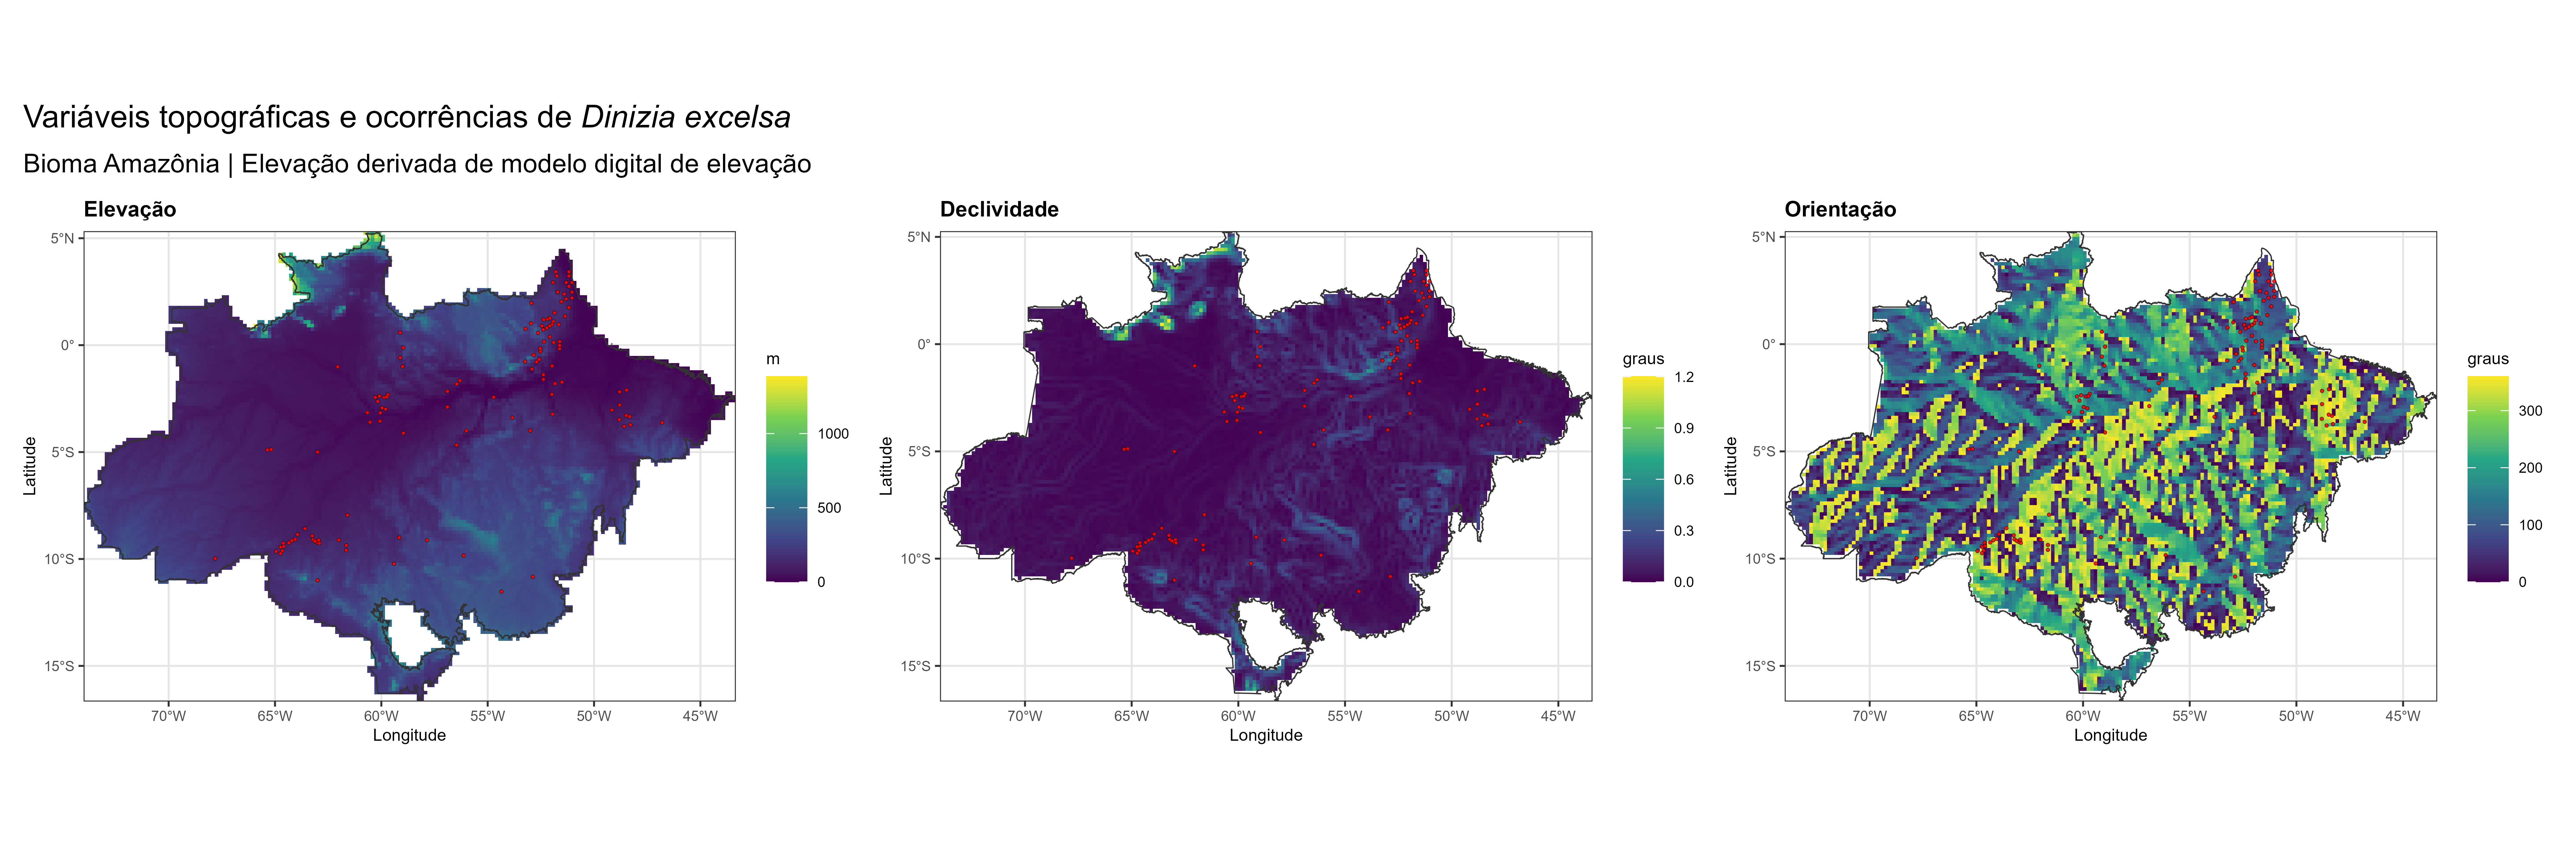
\includegraphics[width=0.98\textwidth]{figuras/unidade03/unidade03_variaveis_topograficas_dinizia.png}
  \caption{Topographic variables prepared for the Amazon biome and the \textit{Dinizia excelsa} case study: elevation, slope, and aspect.}
  \label{fig:unidade03_topografia_dinizia}
\end{figure}

\subsection{Environmental Extraction at Occurrence Locations}

After layer preparation, the value of every predictor is extracted at each
final occurrence location. This environmental matrix characterizes the
species' occupied range, supports correlation analysis and predictor selection,
and provides input for suitability models.

\begin{figure}[H]
  \centering
  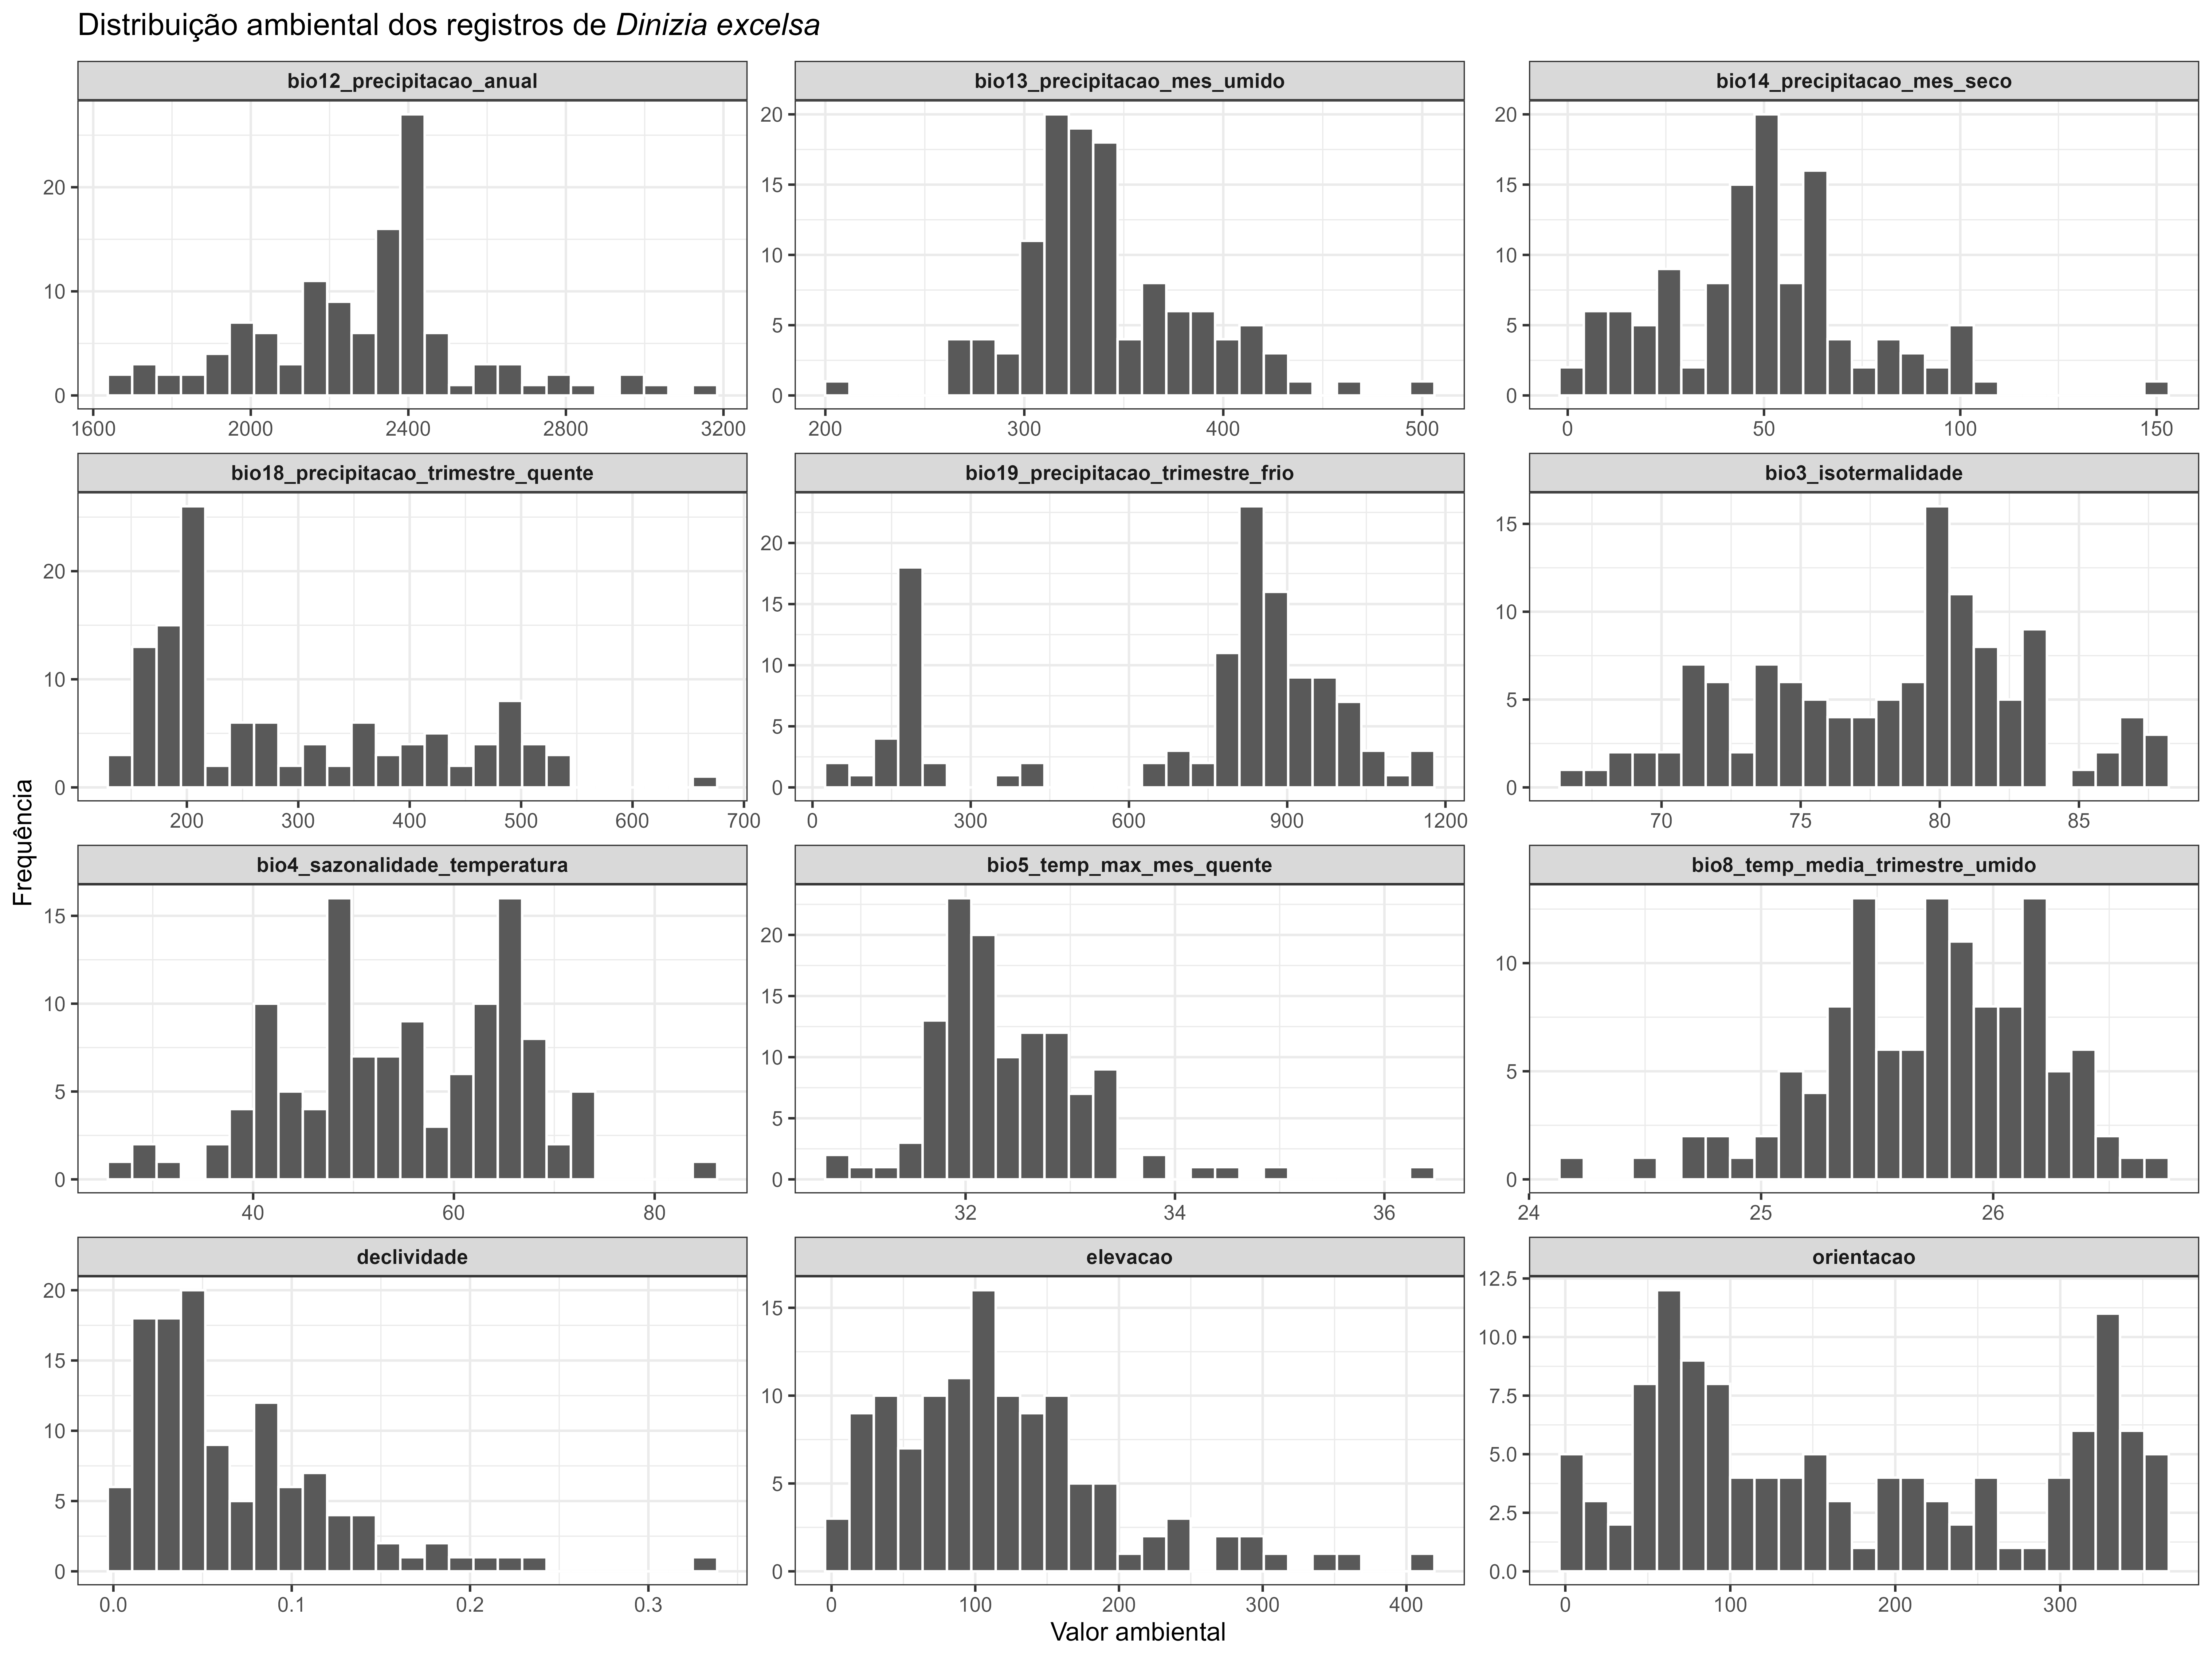
\includegraphics[width=0.94\textwidth]{figuras/unidade03/unidade03_histogramas_ambientais_dinizia.png}
  \caption{Distributions of environmental variables extracted at final \textit{Dinizia excelsa} occurrences. The histograms characterize the environmental range occupied by the species.}
  \label{fig:unidade03_histogramas_dinizia}
\end{figure}

\section{Outputs from Chapter 3}

The chapter script produces:

\begin{itemize}
  \item a multivariate raster of selected bioclimatic variables for Amazonia;
  \item a raster of harmonized topographic variables;
  \item the complete environmental stack used in later chapters;
  \item a table of environmental values at \textit{Dinizia excelsa} occurrences;
  \item an environmental background sample for the Amazon biome;
  \item environmental-layer metadata; and
  \item bioclimatic maps, topographic maps, and environmental histograms.
\end{itemize}

\begin{dica}[title={\faLightbulb\quad File organization}]
Retain these outputs for subsequent chapters. The stack saved as
\texttt{dados/unidade03/processados/variaveis\_ambientais\_amazonia\_unidade03.tif}
is used for multicollinearity analysis, variable selection, model fitting, and
projection.
\end{dica}

\section{Chapter Summary}

Environmental variables connect ecological niches to spatial modeling. Their
selection requires ecological knowledge, consistency with the scale of the
question, compatibility with occurrence records, and technically sound spatial
processing. WorldClim, CHELSA, EarthEnv, ENVIREM, SoilGrids, and SRTM are highly
useful resources, but must be used critically.

For \textit{Dinizia excelsa}, preparing environmental layers across Amazonia
created a reproducible spatial foundation for multicollinearity analysis,
variable selection, model fitting, and maps of present, past, and future
suitability.

\begin{conceito}[title={\faBook\quad Key message}]
Environmental variables in SDM are not merely map layers. They represent
ecological hypotheses about the factors that limit, favor, or structure species
distributions.
\end{conceito}

\section{Review Exercises}

\begin{enumerate}
  \item Explain the difference between geographic and environmental space.
  \item Why does an important predictor not necessarily represent a causal ecological mechanism?
  \item Distinguish spatial resolution, geographic extent, and ecological scale.
  \item Why are climatic variables widely used in broad-scale SDM?
  \item Give examples of topographic predictors relevant to species distributions.
  \item Explain the importance of edaphic variables in plant distribution models.
  \item Why must environmental layers be harmonized before modeling?
  \item Which predictors might represent water availability for \textit{Dinizia excelsa}?
  \item Why must rasters share resolution, extent, and CRS before modeling?
\end{enumerate}

\chapter[Multicollinearity]{Multicollinearity in Species Distribution Modeling}

\begin{objetivos}
By the end of this chapter, readers should be able to explain multicollinearity
in SDM; identify redundant environmental variables using correlation; calculate
and interpret the variance inflation factor (VIF); understand the effects of
collinearity on ecological interpretation, parameter stability, and model
transferability; use principal component analysis (PCA) for dimensionality
reduction; and build a reproducible R workflow for selecting or transforming
environmental predictors before model fitting.
\end{objetivos}

\section{Introduction}

Multicollinearity occurs when two or more predictors carry similar information.
It is common in species distribution modeling because climatic, topographic,
edaphic, and hydrological variables frequently covary across space. Mean annual
temperature may be strongly associated with elevation, annual precipitation
with precipitation of the wettest quarter, and several topographic metrics may
be redundant because they derive from the same digital elevation model.

Strongly correlated predictors can produce unstable models, obscure variable
importance, inflate uncertainty in parametric models, and reduce spatial or
temporal transferability. Environmental-predictor selection should therefore
combine ecological reasoning, exploratory analysis, and statistical criteria
\parencite{guisan2017habitat,naimi2016sdm,raes2018modeling}.

\begin{atencao}[title={\faExclamationTriangle\quad More predictors do not necessarily produce a better model}]
Adding many environmental variables does not guarantee improved performance.
Redundant predictors may increase complexity, generate instability, hinder
ecological interpretation, and reduce transferability.
\end{atencao}

\section{The Multicollinearity Problem}

Environmental predictors often show strong mutual correlation. In tropical
regions, for example, high annual precipitation may coincide with low water
seasonality, while thermal gradients may follow elevation.

When two or more predictors carry similar information, multicollinearity
arises. Predictive performance may remain high, but ecological interpretation
of coefficients becomes unstable and spatial or temporal transfer may be
compromised \parencite{dormann2013collinearity}.

\section{Correlation Among Environmental Variables}

The simplest redundancy diagnostic is pairwise correlation. Pearson and
Spearman coefficients are the most common in SDM. Pearson measures linear
association between continuous variables. Spearman measures rank-based
monotonic association and is useful for nonnormal or skewed distributions.

Operational thresholds such as \(|r| > 0.7\) or \(|r| > 0.8\) are often used to
flag strong correlation. They are not universal rules. When two variables are
strongly correlated, preference should be given to the one with greater
ecological relevance, higher spatial quality, clearer interpretation, or better
alignment with the study objective
\parencite{dormann2013collinearity,raes2018modeling}.

\begin{conceito}[title={\faBook\quad Correlation is not causation}]
Two variables can be strongly correlated without either causing the other. In
SDM, correlation indicates shared information, but ecological knowledge and the
study hypothesis should determine which variable is retained.
\end{conceito}

\begin{conceito}[title={\faBook\quad Statistical correlation does not imply ecological redundancy}]
Strongly correlated variables may still represent distinct ecological
processes. Annual precipitation and precipitation of the driest quarter, for
example, may be correlated while representing different mechanisms related to
water availability.
\end{conceito}

\rscriptfile{scripts/unidade04/01_estrutura_pastas.R}
\rscriptfile{scripts/unidade04/02_preparar_variaveis_colineares.R}
\rscriptfile{scripts/unidade04/03_correlacao_variaveis.R}

\begin{figure}[H]
  \centering
  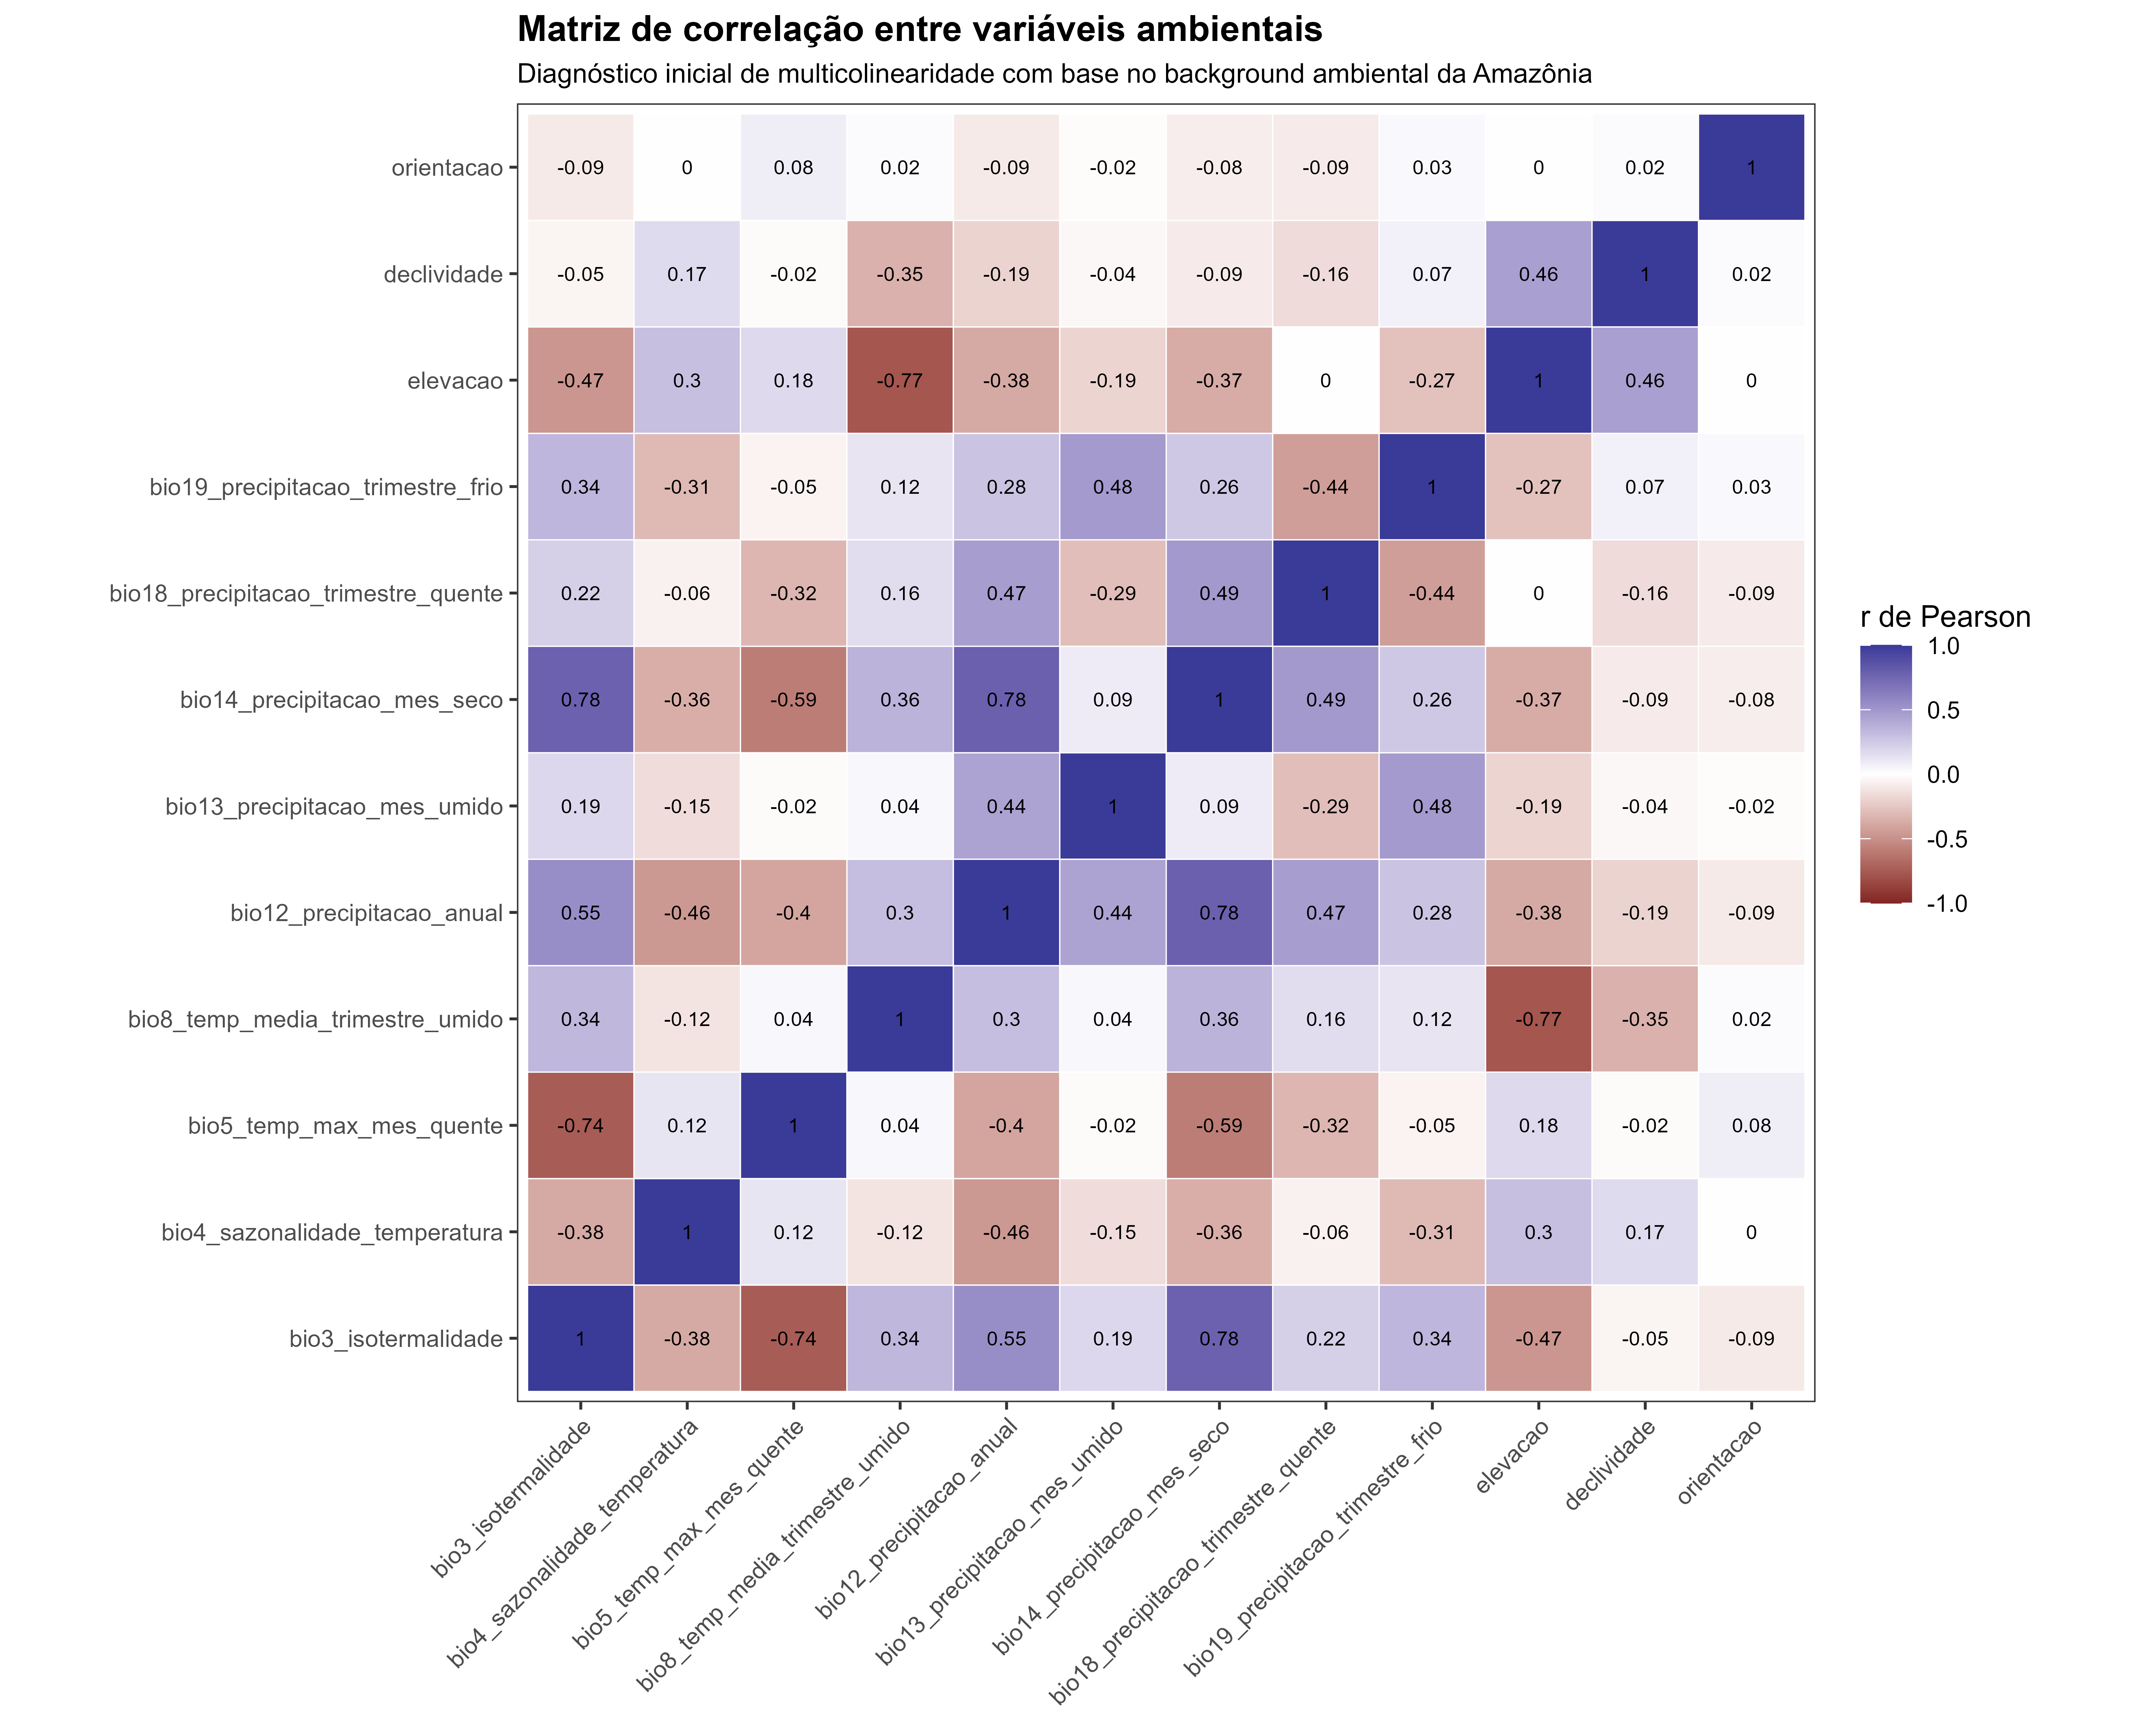
\includegraphics[width=\textwidth]{figuras/unidade04/unidade04_matriz_correlacao.png}
  \caption{Pearson correlation matrix for the environmental variables used to model \textit{Dinizia excelsa} across the Amazon biome. Coefficients indicate the strength of linear association between pairs of predictors.}
  \label{fig:unidade04_matriz_correlacao}
\end{figure}

\section{Variance Inflation Factor}

The variance inflation factor assesses how much the estimated variance of a
coefficient is inflated by linear dependence between one predictor and all
others. Unlike pairwise correlation, VIF evaluates each variable in relation to
the complete predictor set.

\begin{equationbox}
\[
VIF_j = \frac{1}{1 - R_j^2}
\]
Here, \(VIF_j\) is the variance inflation factor for predictor \(j\), and
\(R_j^2\) is the coefficient of determination from regressing predictor \(j\)
on all remaining predictors.
\end{equationbox}

High VIF indicates that a variable can be explained by a combination of the
others. A VIF above 10 is frequently interpreted as severe collinearity,
although more conservative thresholds such as 5 are also used in ecological
studies \parencite{obrien2007vif,dormann2013collinearity,naimi2016sdm}.

\begin{dica}[title={\faLightbulb\quad Correlation and VIF are complementary}]
Correlation identifies redundant pairs; VIF identifies redundancy relative to
the complete predictor set. Robust studies should examine both diagnostics.
\end{dica}

\rscriptfile{scripts/unidade04/04_vif_variaveis.R}

\begin{figure}[H]
  \centering
  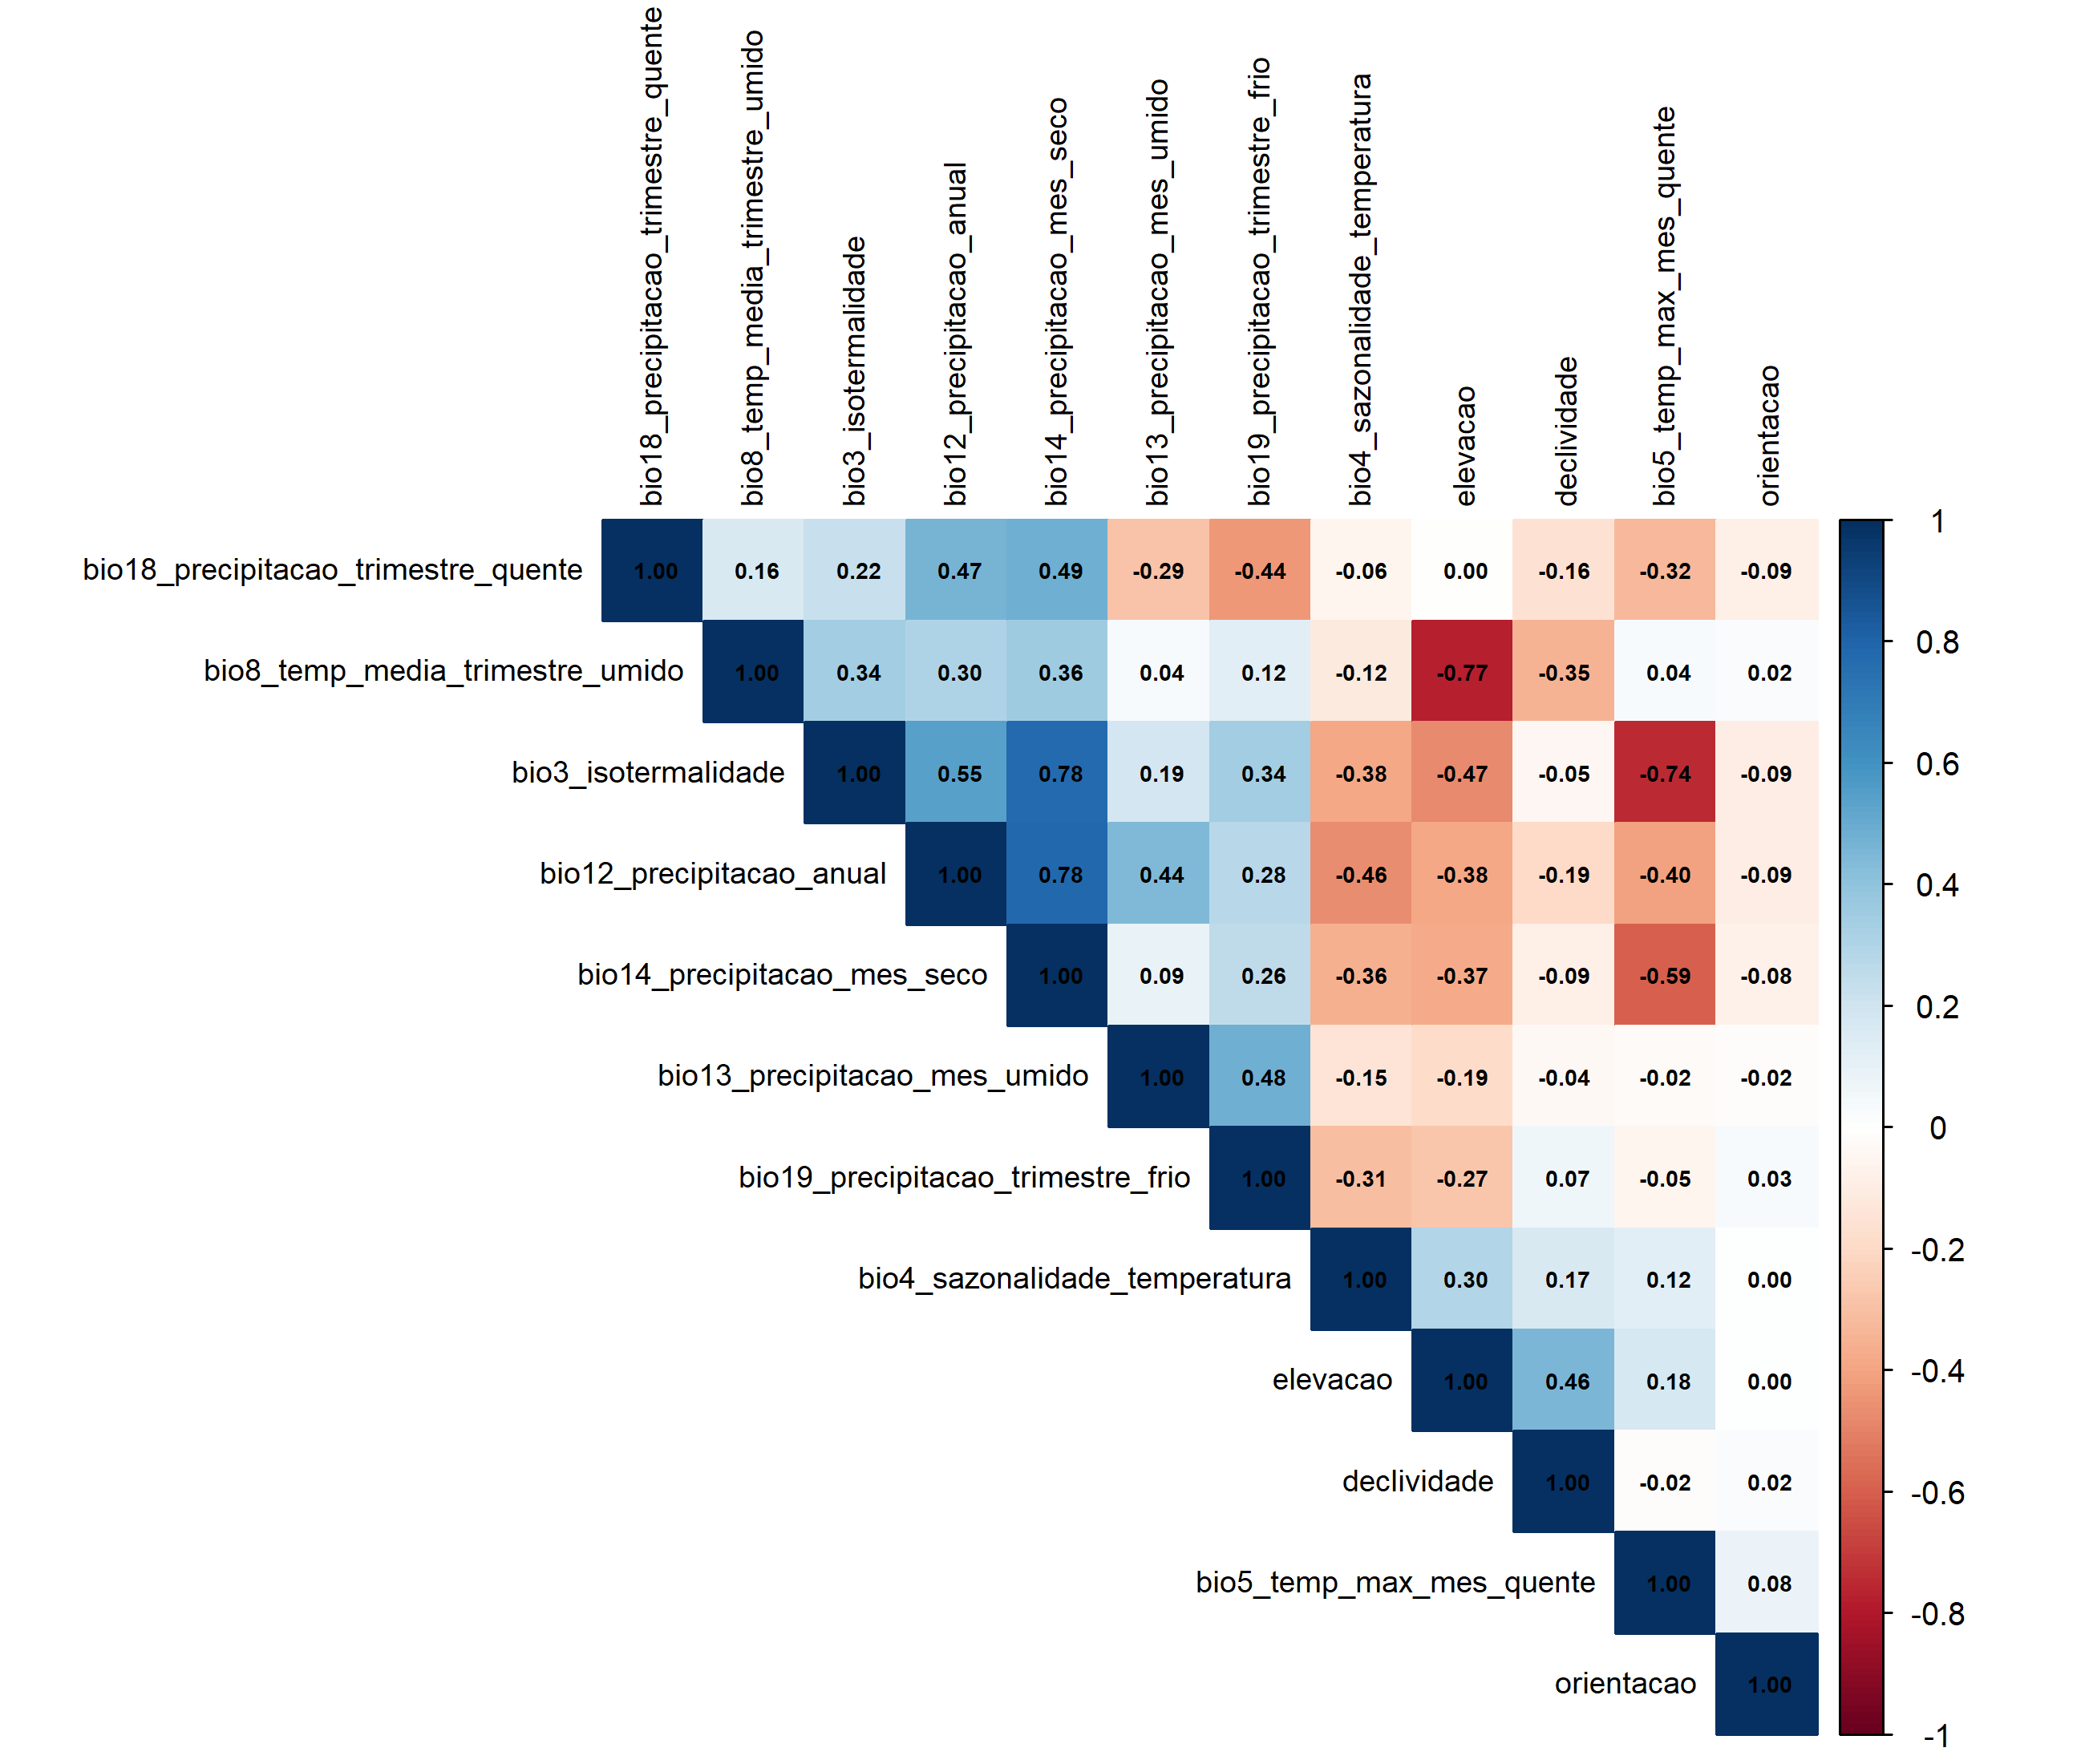
\includegraphics[width=0.95\textwidth]{figuras/unidade04/unidade04_corrplot_correlacao.png}
  \caption{Graphical representation of correlations among environmental variables. More intense colors denote stronger correlations, whereas values near zero indicate greater independence.}
  \label{fig:unidade04_corrplot}
\end{figure}

\begin{figure}[H]
  \centering
  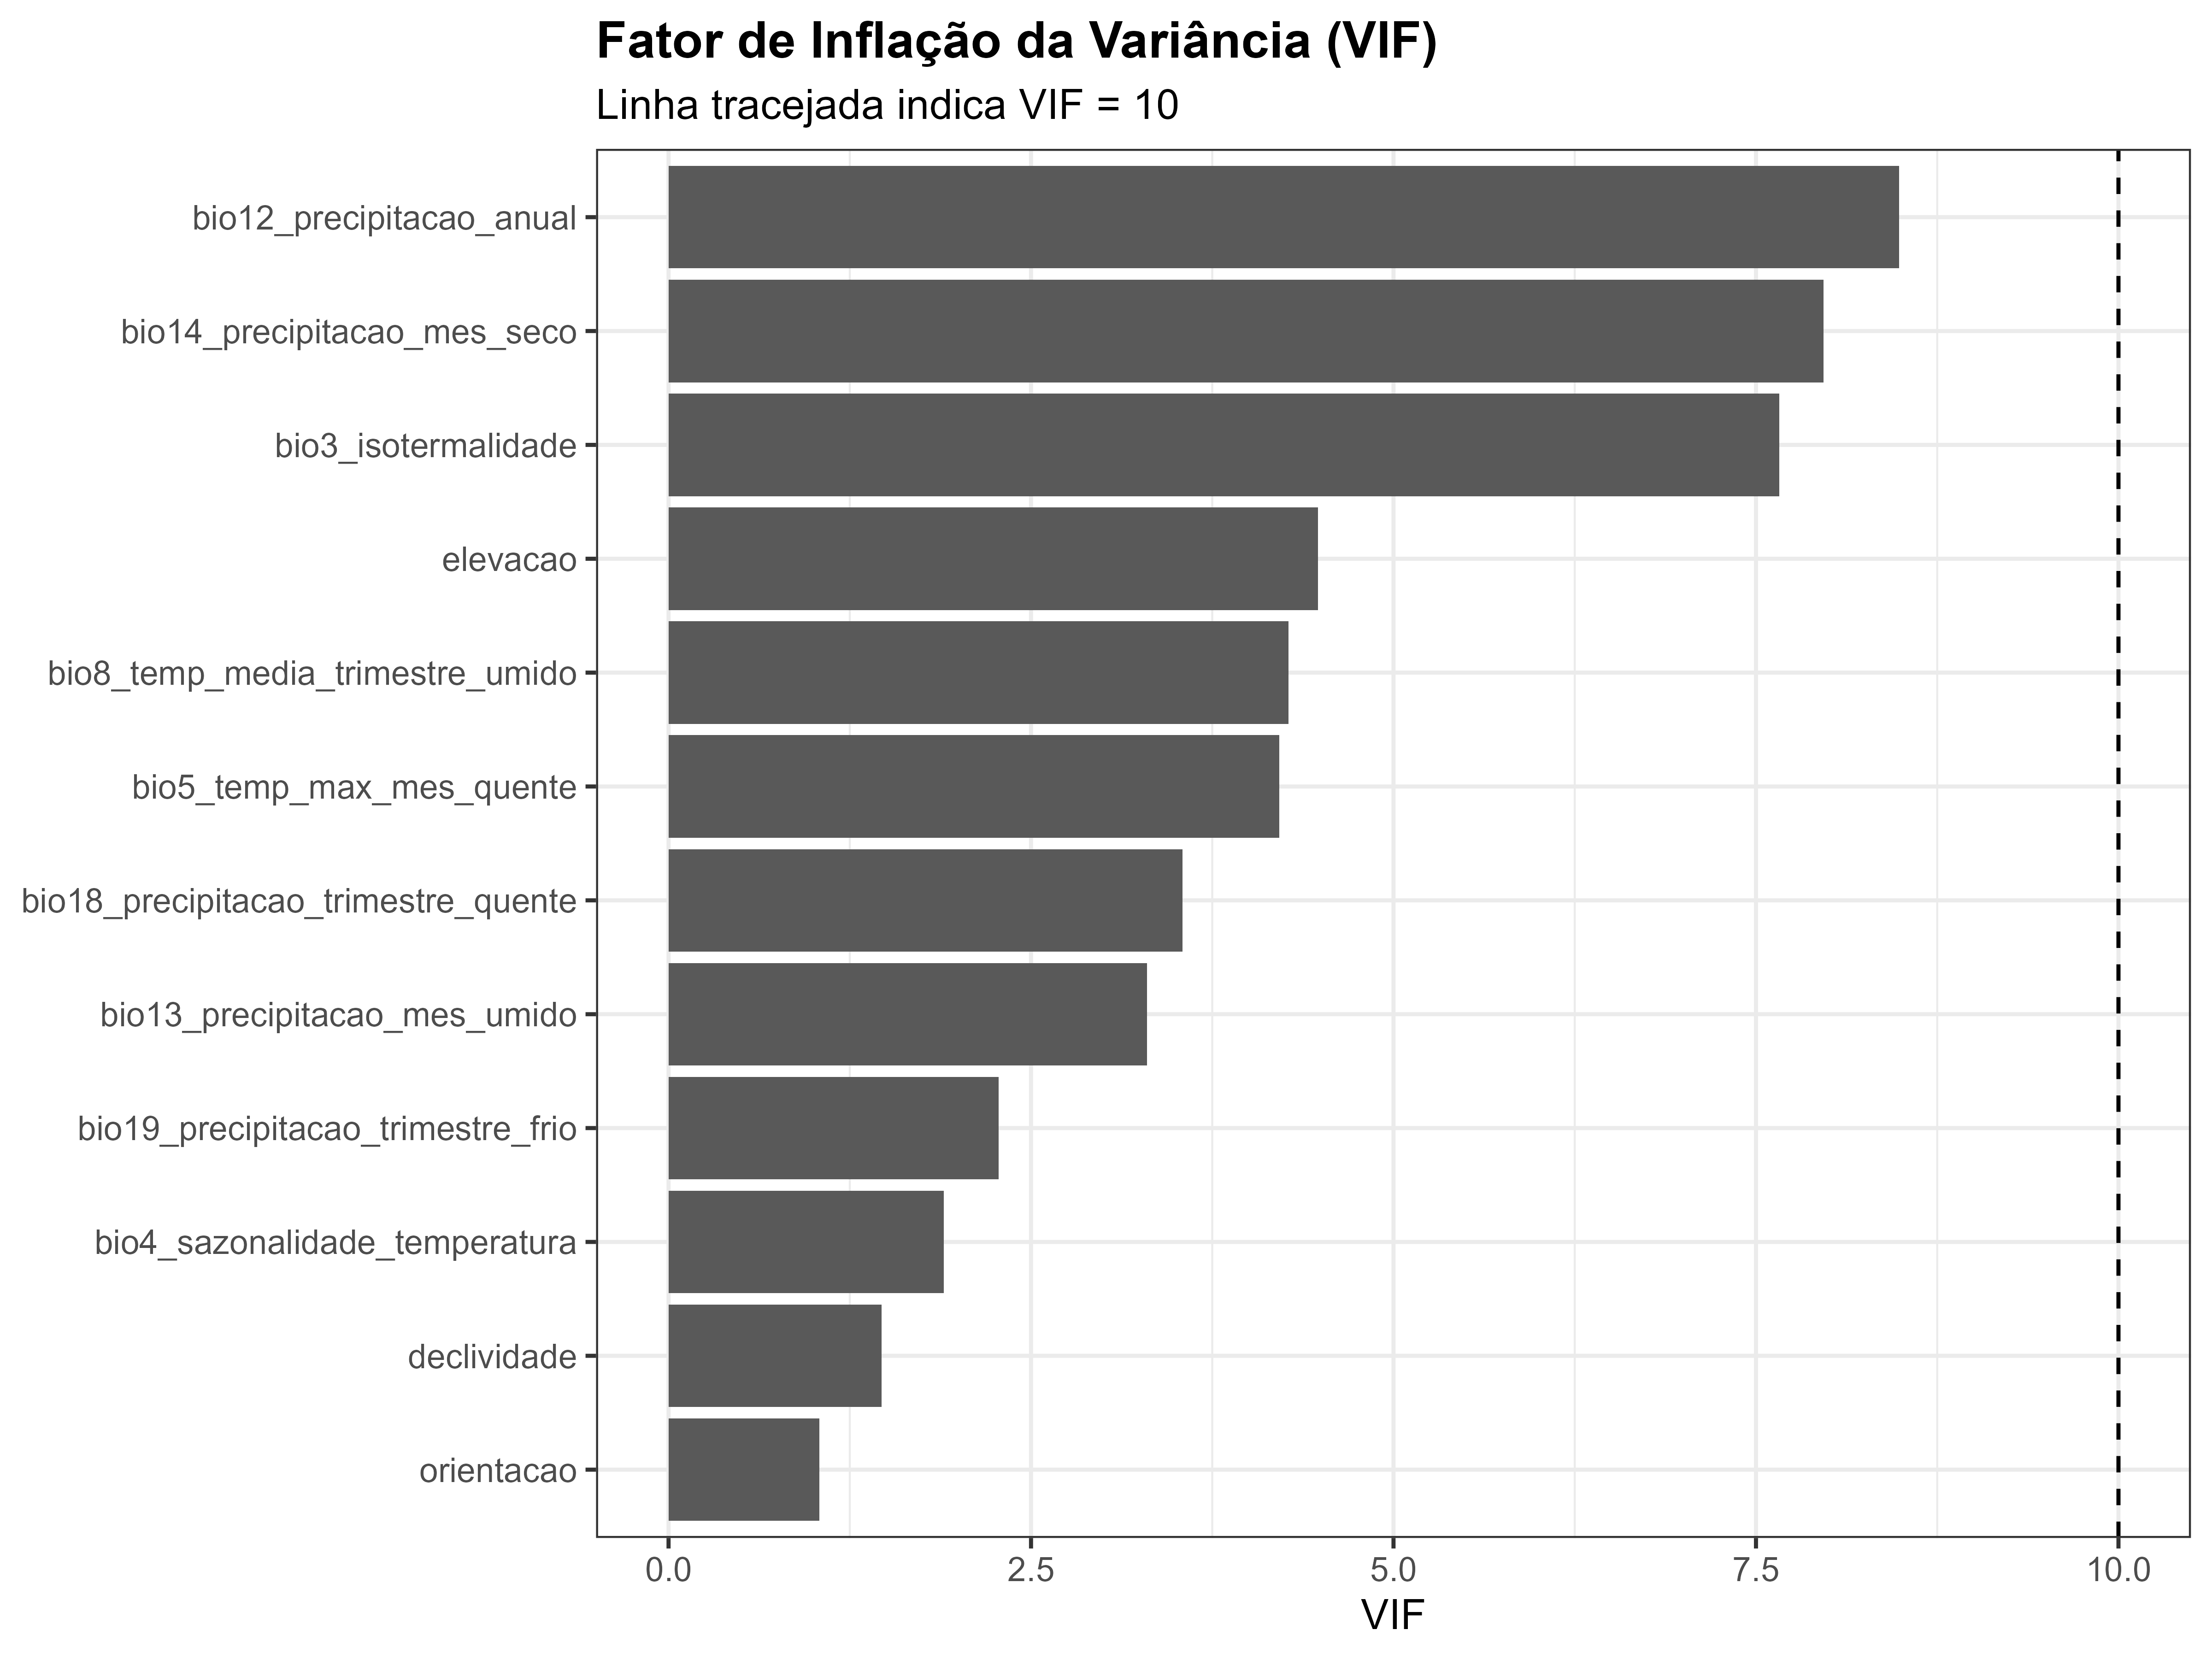
\includegraphics[width=0.85\textwidth]{figuras/unidade04/unidade04_vif_variaveis.png}
  \caption{Variance inflation factor values for the evaluated environmental variables. The dashed line is the operational threshold used to identify excessive multicollinearity.}
  \label{fig:unidade04_vif}
\end{figure}

\begin{aplicacao}
Figures~\ref{fig:unidade04_matriz_correlacao} and
\ref{fig:unidade04_corrplot} identify groups of variables carrying similar
information. Retaining strongly correlated predictors can impede ecological
interpretation and destabilize spatial and temporal projections.
\end{aplicacao}

\begin{aplicacao}
VIF quantifies how much the variance associated with a predictor is inflated by
correlation with other predictors. High values indicate statistical redundancy
and suggest removing the variable or replacing it with a more ecologically
representative alternative.
\end{aplicacao}

\section{Selecting Environmental Variables}

Variable selection must balance ecological relevance, data quality, and
statistical redundancy. Automatic removal based solely on thresholds can yield
ecologically weak models, whereas retaining redundant variables makes models
difficult to interpret.

A useful workflow begins with a broad candidate set, provides an ecological
justification for each predictor group, and then applies correlation and VIF
filters. When variables are correlated, priority should be given to the one
more directly linked to ecological processes, more stable through time, better
resolved, or subject to less measurement error.

\begin{atencao}[title={\faExclamationTriangle\quad Do not let the algorithm alone select the predictors}]
Automated selection may discard ecologically important variables while
retaining statistically convenient but biologically fragile ones. Predictor
selection must be documented and justified.
\end{atencao}

\rscriptfile{scripts/unidade04/05_selecao_variaveis.R}

\begin{figure}[H]
  \centering
  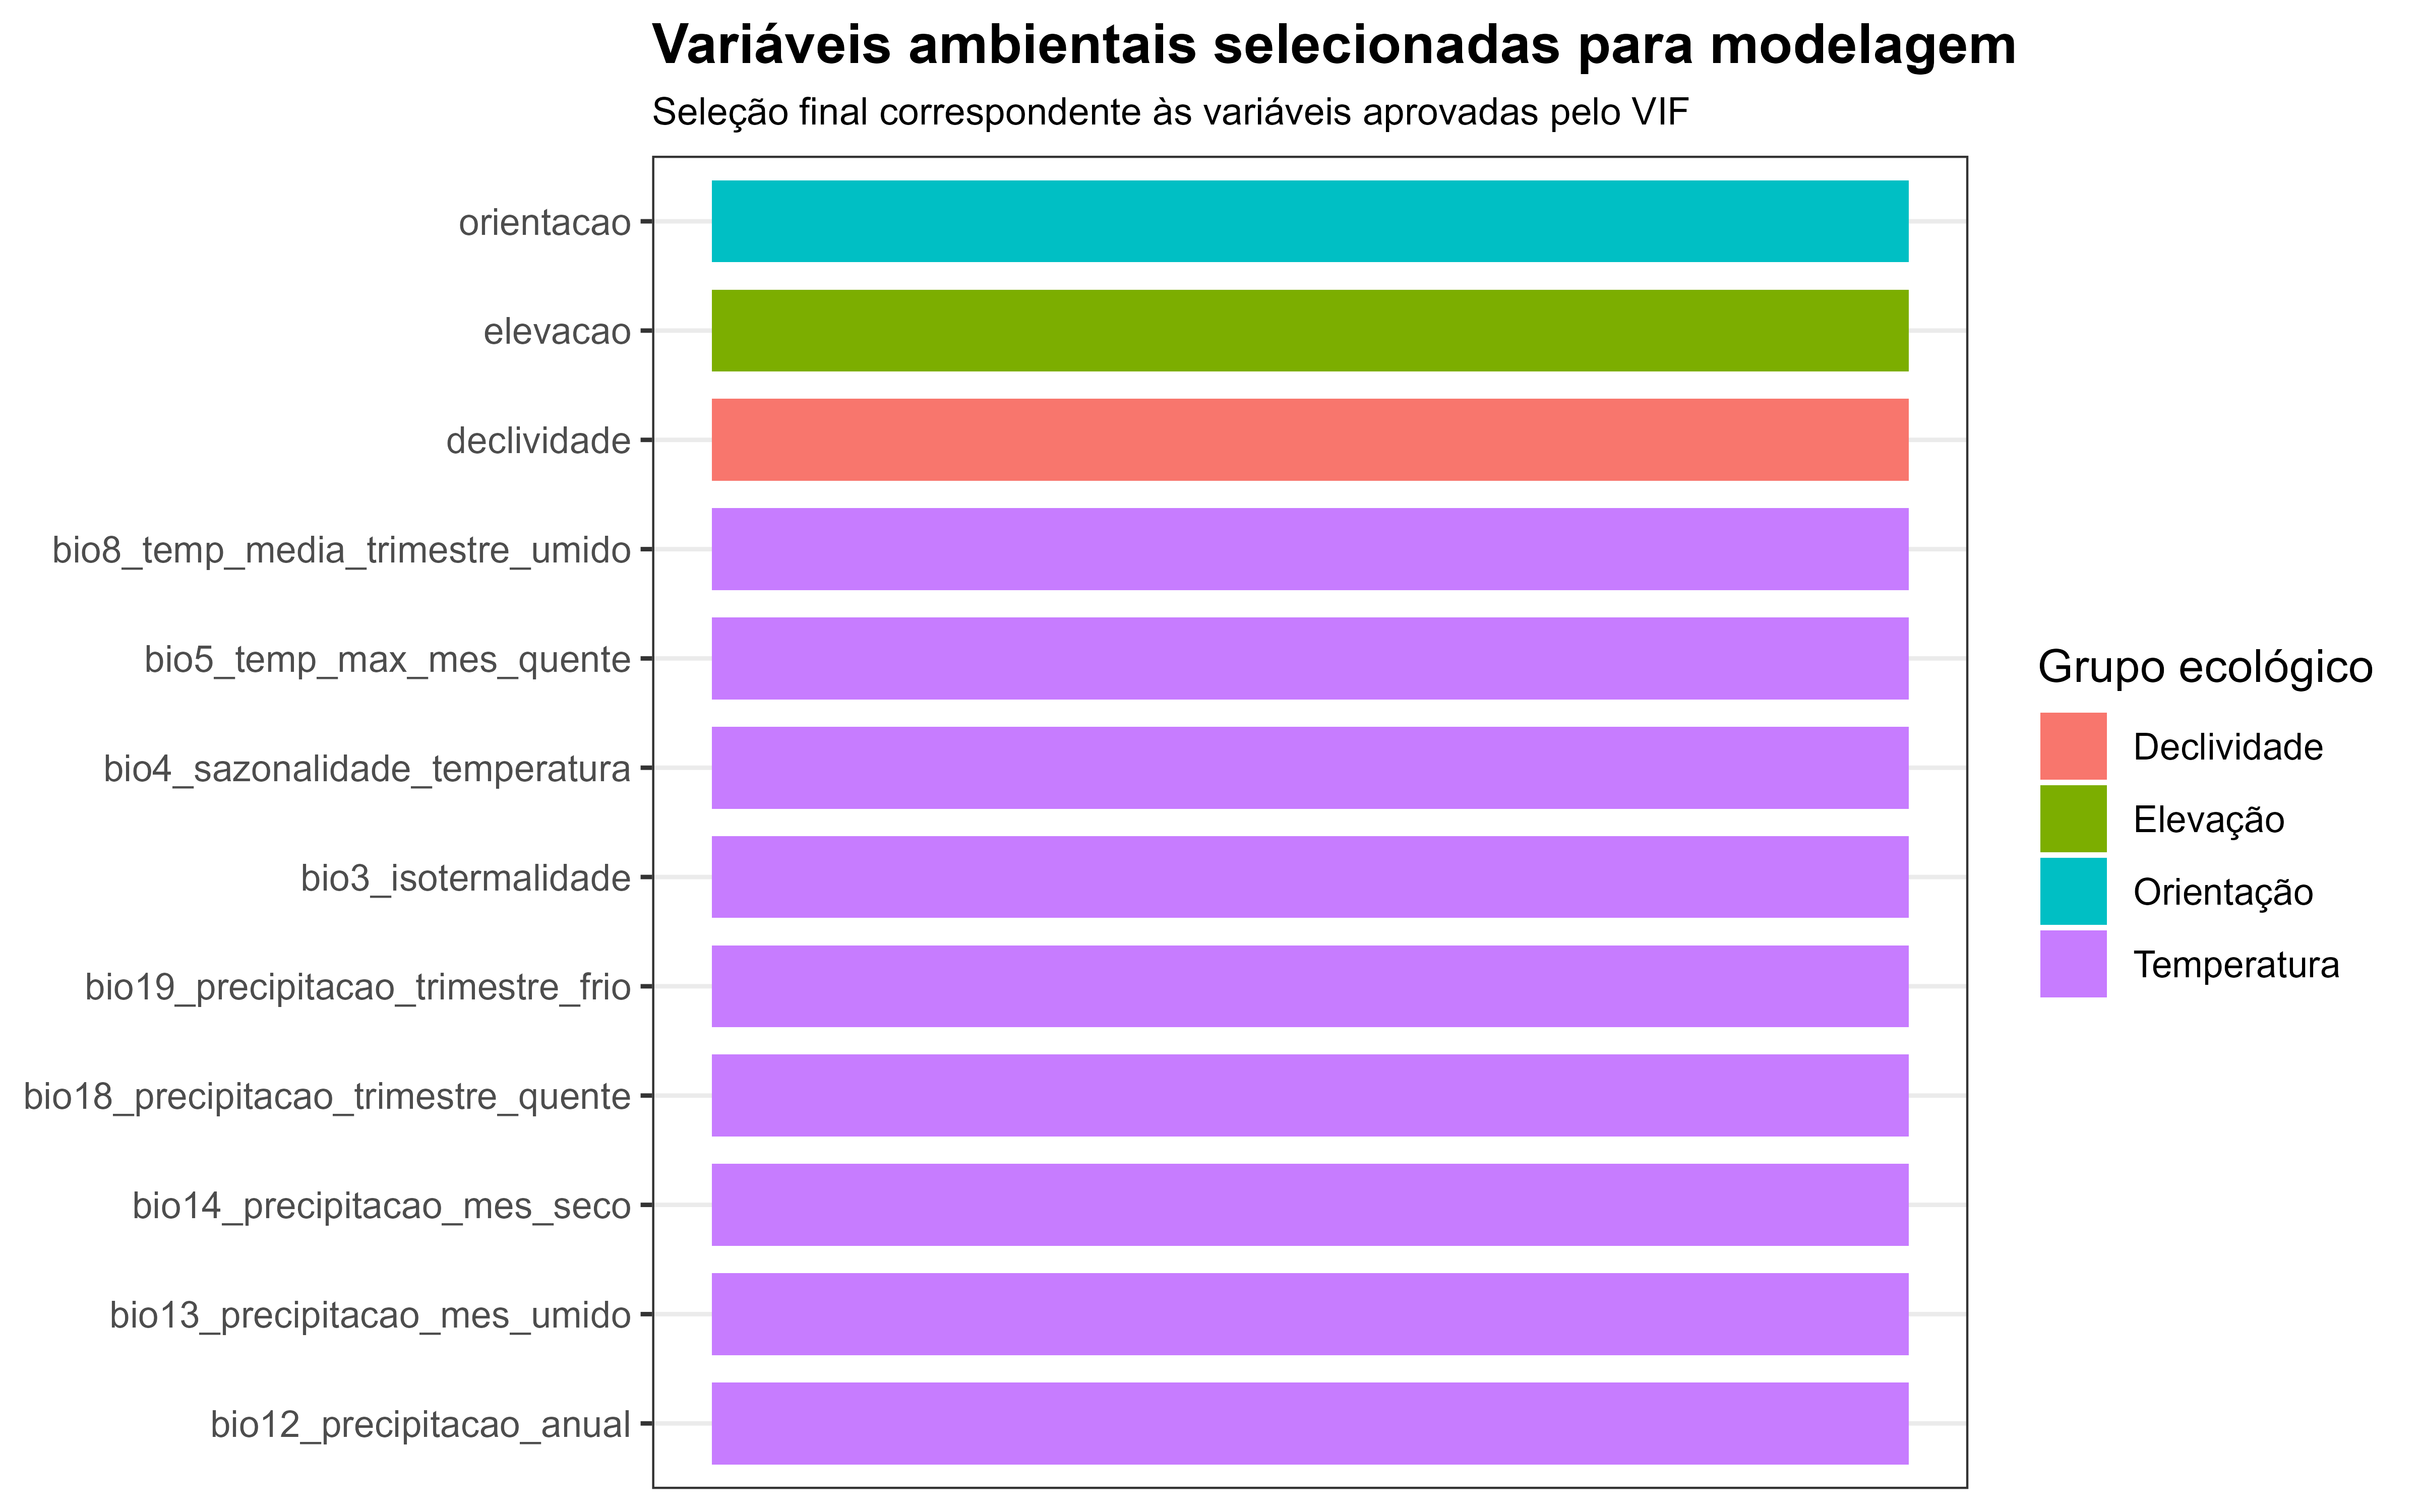
\includegraphics[width=0.85\textwidth]{figuras/unidade04/unidade04_variaveis_selecionadas.png}
  \caption{Final environmental predictors selected after correlation analysis, VIF diagnosis, and ecological interpretation. These variables are used to fit species distribution models in subsequent chapters.}
  \label{fig:unidade04_variaveis_final}
\end{figure}

\section{PCA in Species Distribution Modeling}

Principal component analysis is a dimensionality-reduction method that
transforms correlated variables into orthogonal axes. These principal
components are uncorrelated linear combinations of the original variables.

PCA can provide a compact representation of environmental space when
collinearity is strong. Its disadvantage is reduced direct ecological
interpretability: a component represents a combination of variables rather than
a simple gradient such as temperature or precipitation.

\begin{conceito}[title={\faBook\quad PCA as orthogonalization}]
PCA does not select variables. It transforms correlated variables into
independent axes. This reduces collinearity but requires care when interpreting
the resulting components ecologically.
\end{conceito}

\rscriptfile{scripts/unidade04/06_pca_variaveis.R}

\begin{figure}[H]
  \centering
  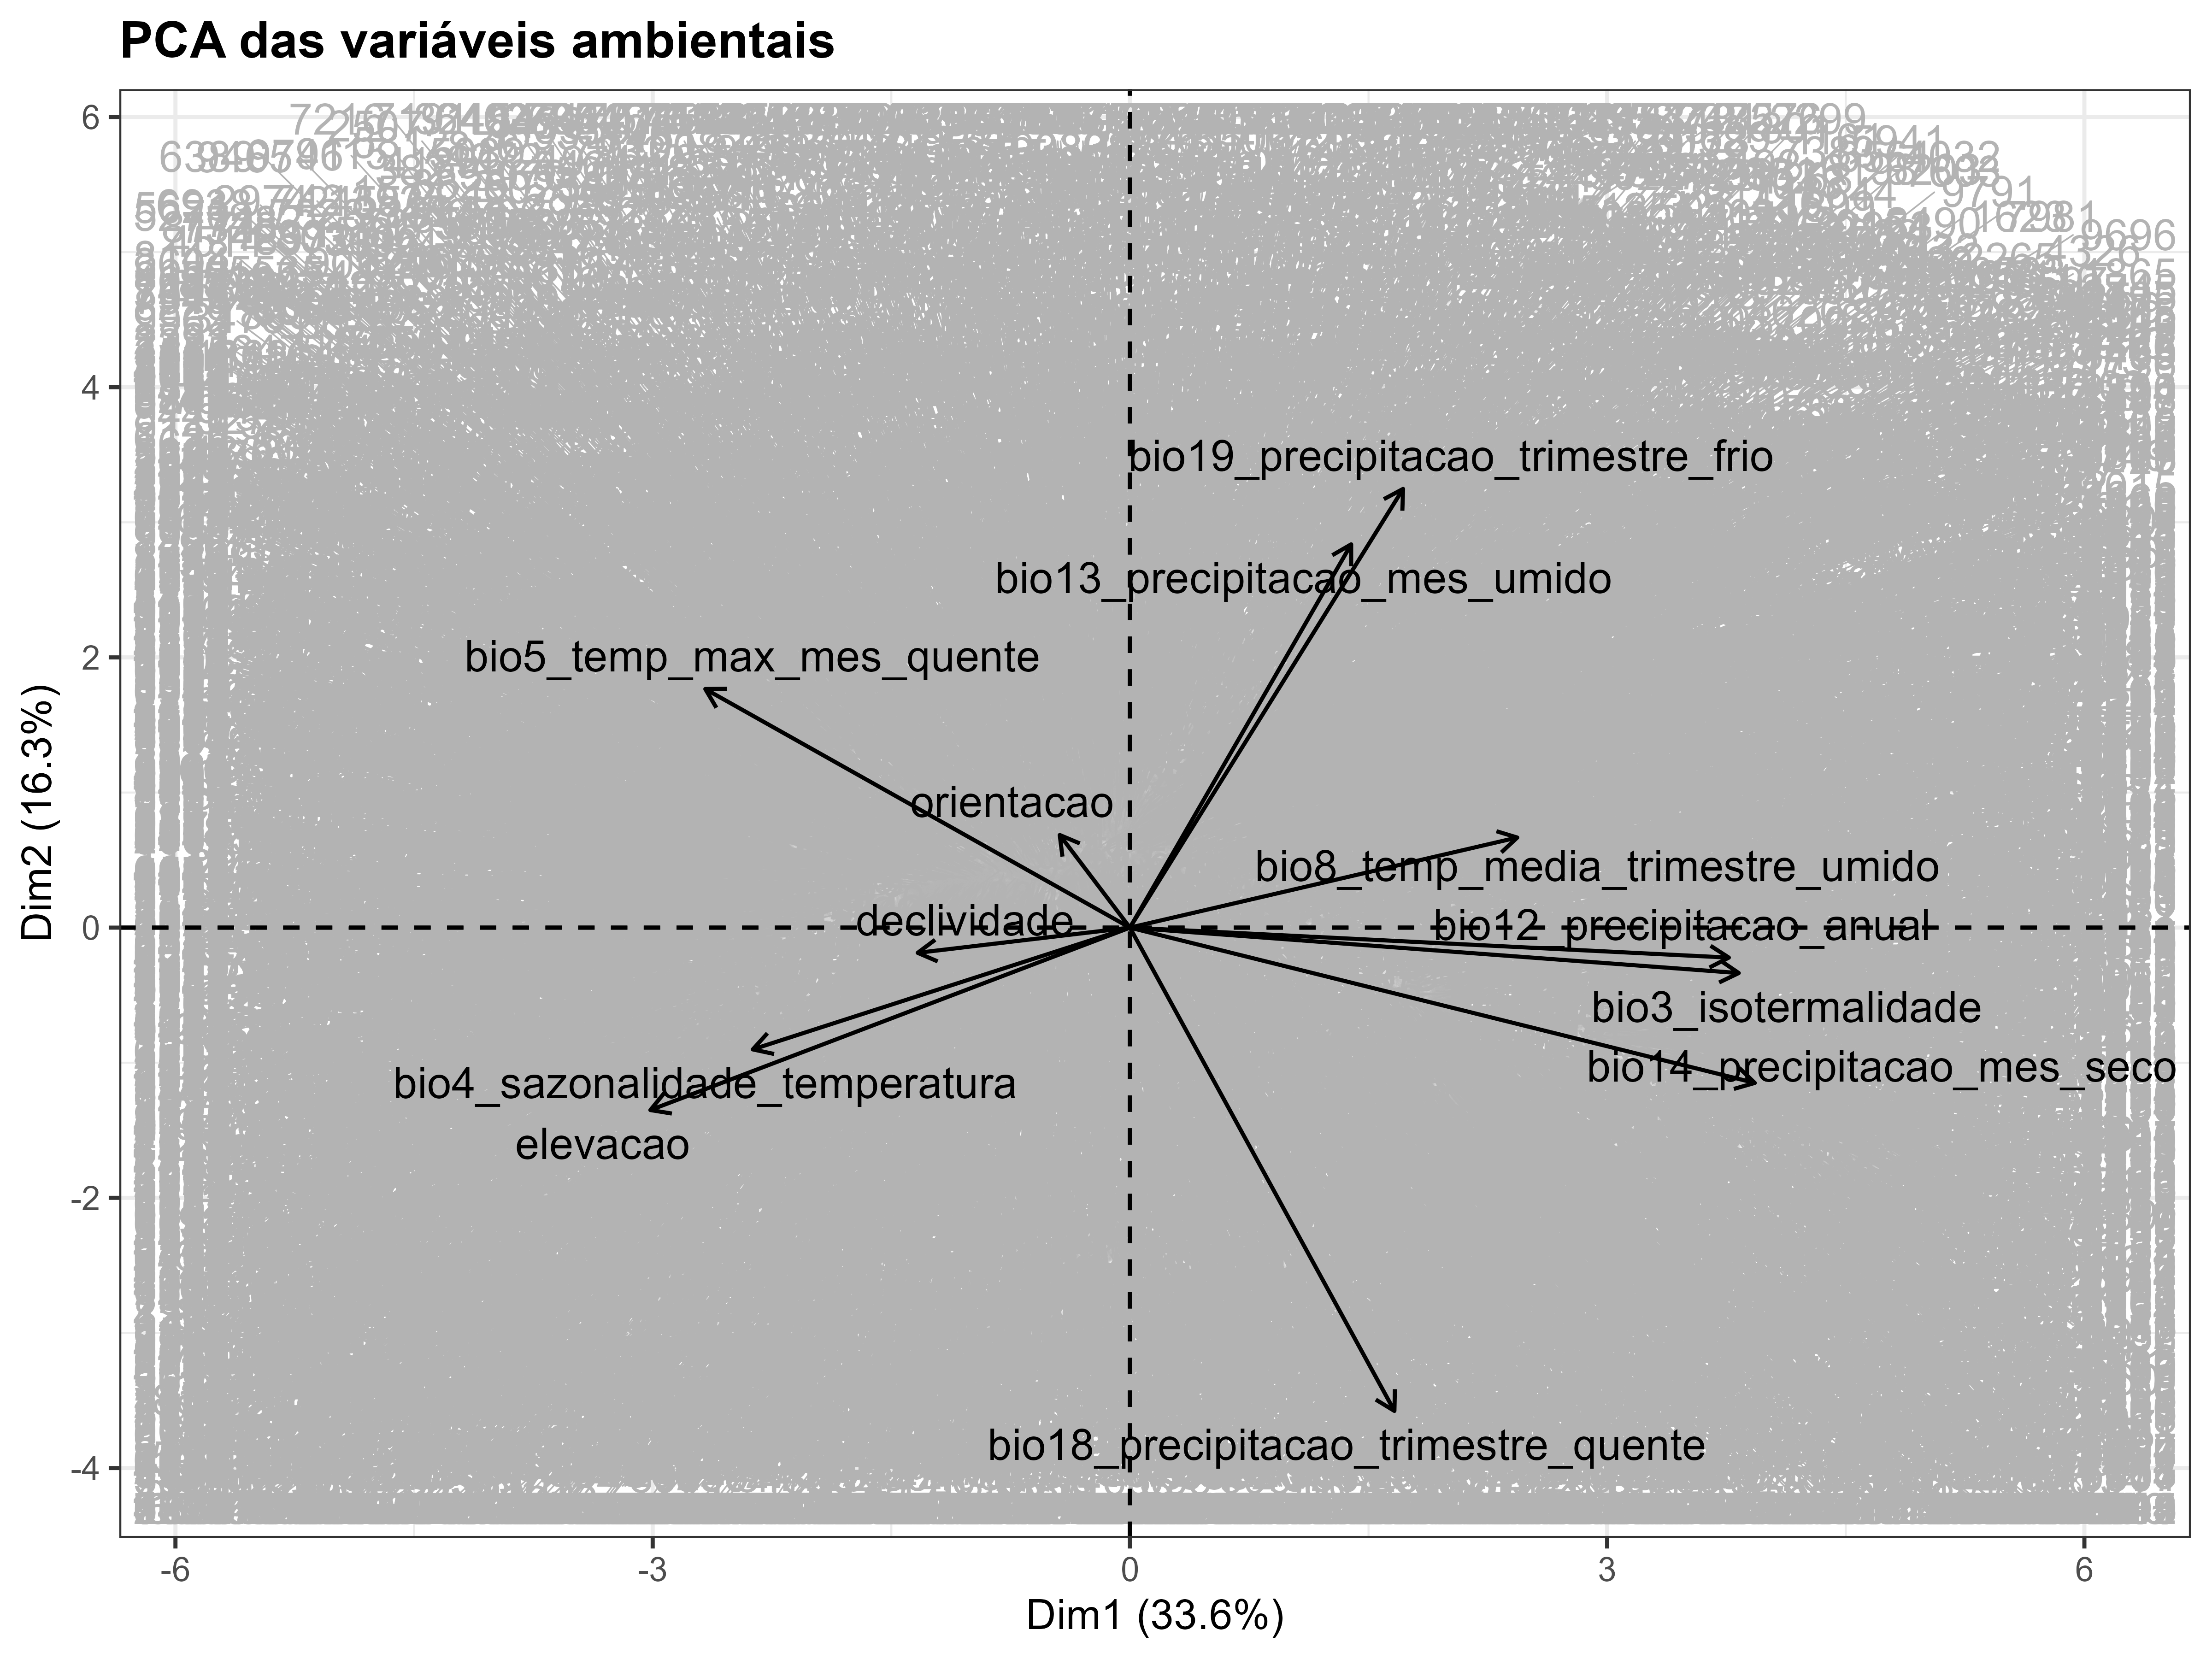
\includegraphics[width=0.90\textwidth]{figuras/unidade04/unidade04_pca_biplot_variaveis.png}
  \caption{Principal component analysis of environmental variables used in the case study. Vectors show the contribution of each variable to the principal environmental gradients of the Amazon biome.}
  \label{fig:unidade04_pca_biplot}
\end{figure}

\begin{figure}[H]
  \centering
  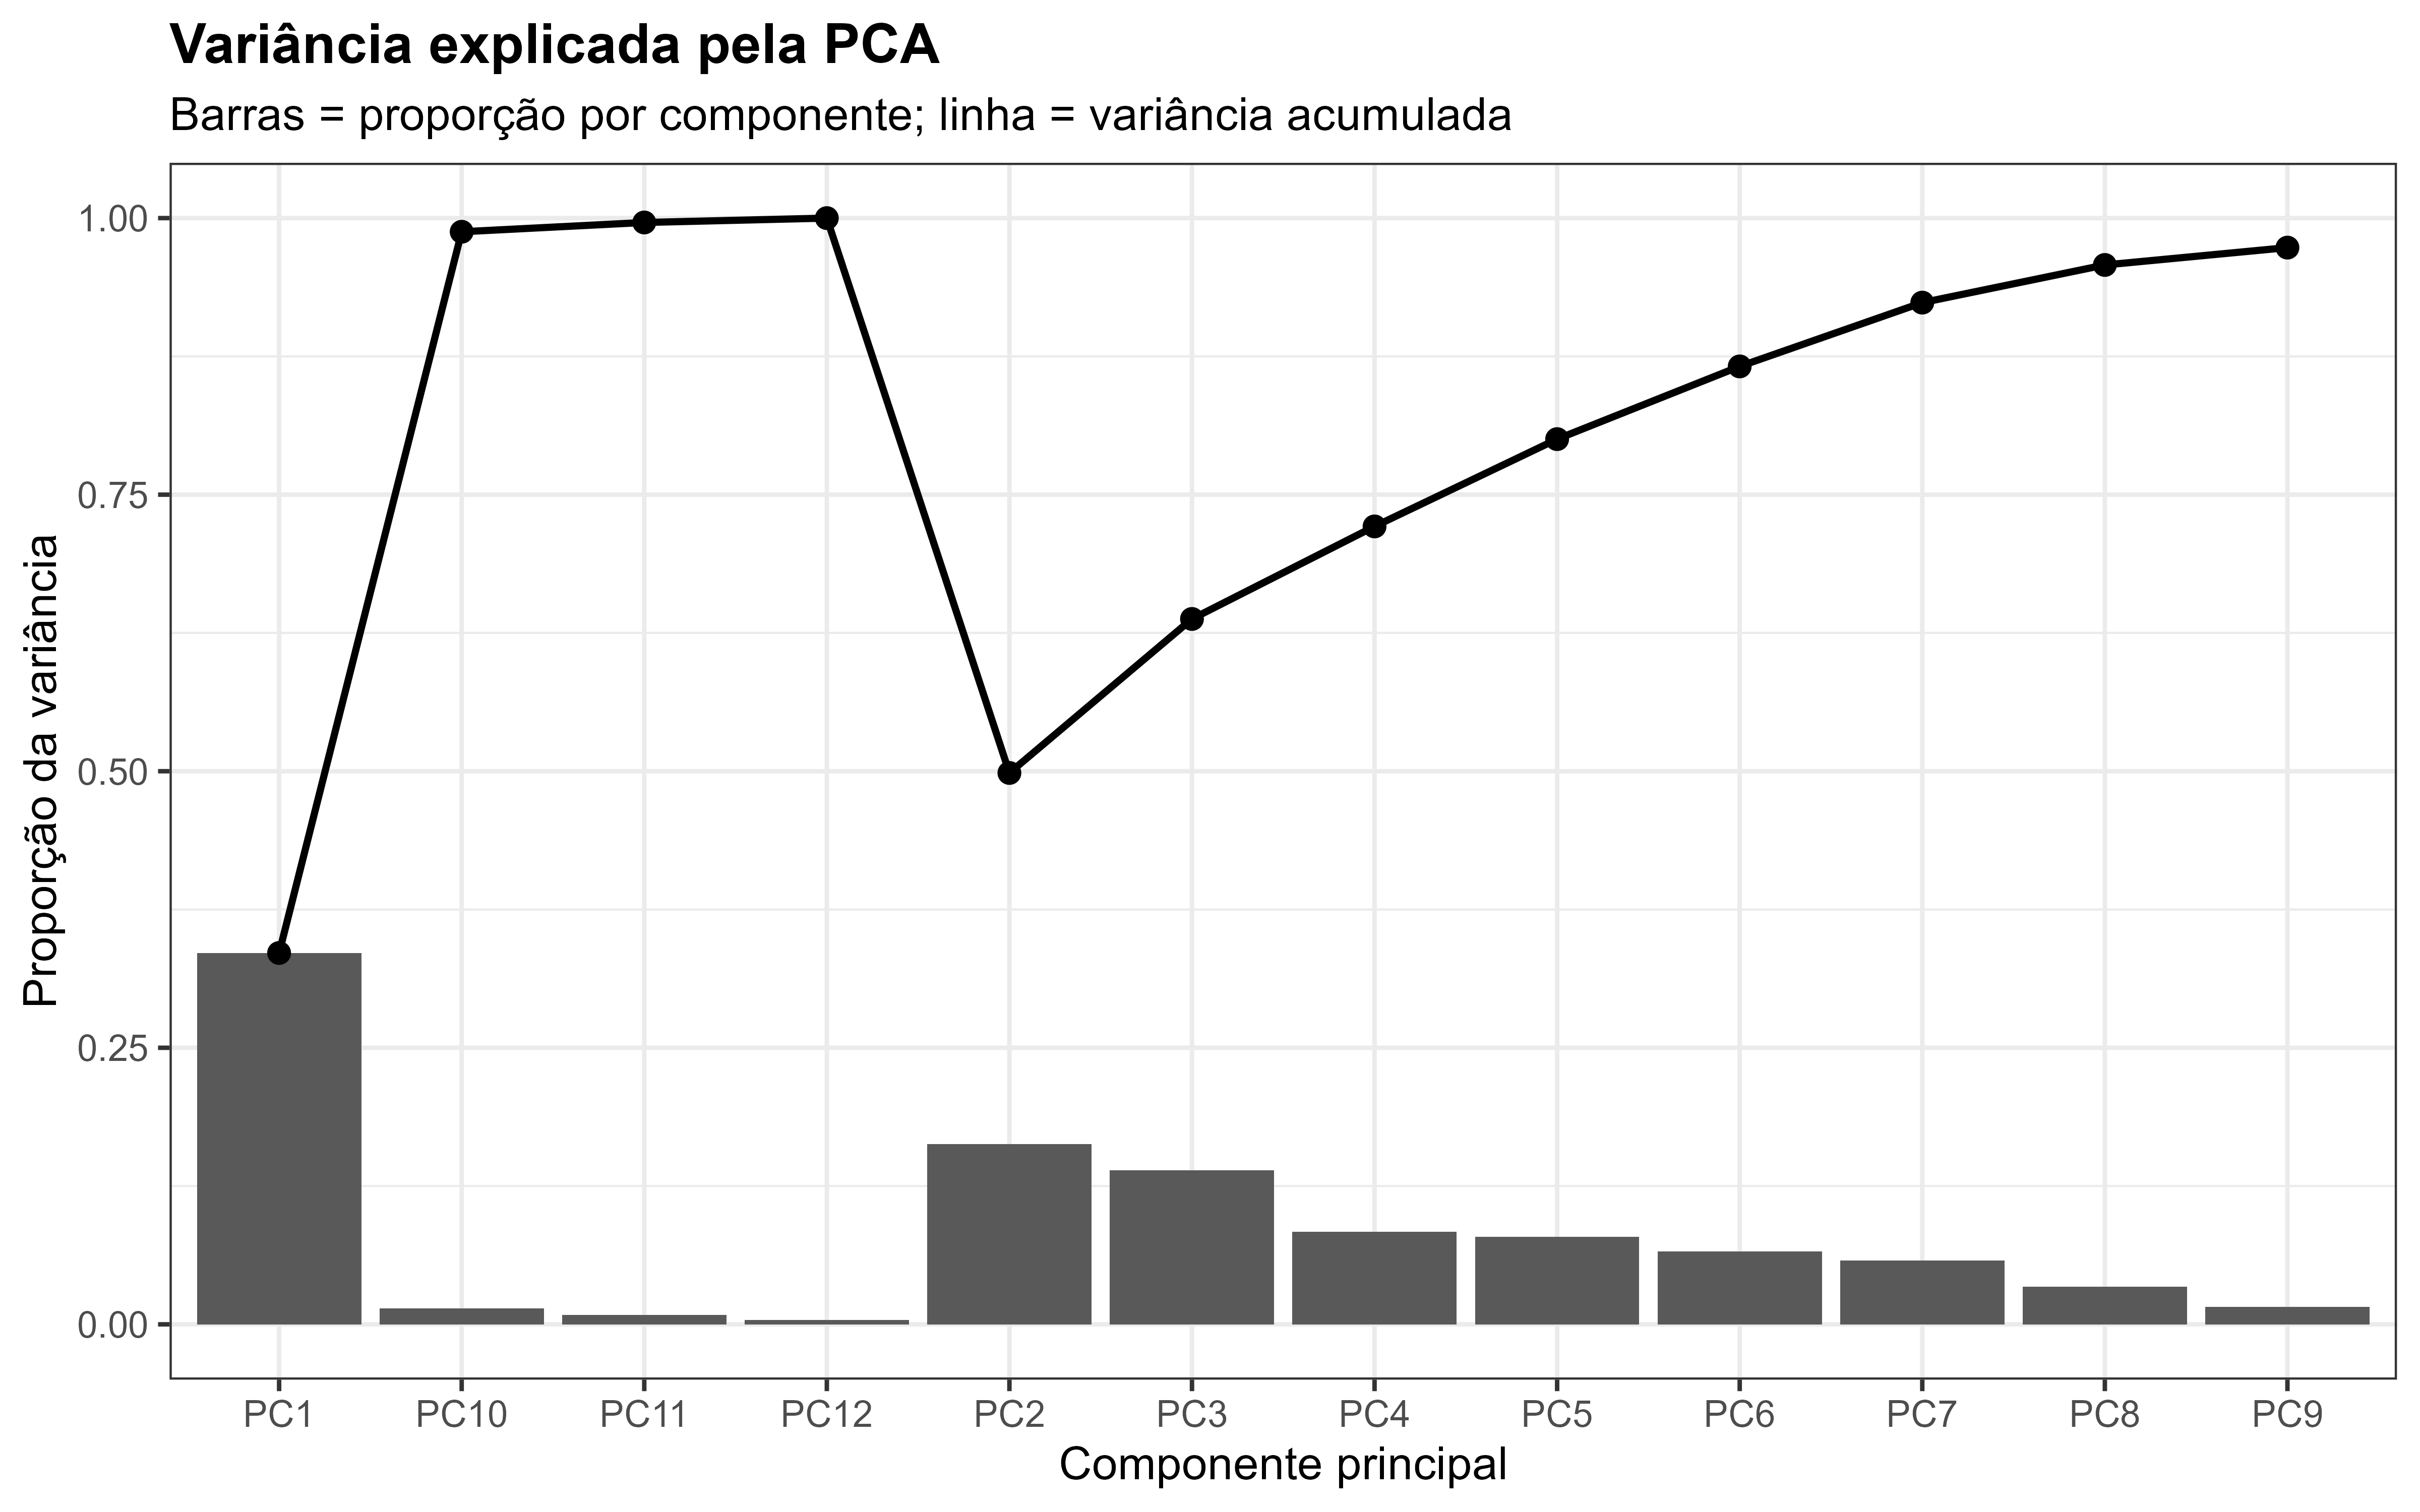
\includegraphics[width=0.80\textwidth]{figuras/unidade04/unidade04_pca_variancia.png}
  \caption{Proportion of variance explained by the principal components. Bars show the contribution of each axis and the line shows cumulative explained variance.}
  \label{fig:unidade04_pca_variancia}
\end{figure}

\begin{aplicacao}
Figures~\ref{fig:unidade04_pca_biplot} and
\ref{fig:unidade04_pca_variancia} show that a small number of principal axes can
represent much of Amazonia's environmental structure. PCA does not replace
ecological variable selection, but helps diagnose redundancy and interpret the
gradients structuring the distribution of \textit{Dinizia excelsa}.
\end{aplicacao}

\section{Integrated Pipeline}

The final script combines all Chapter 4 steps: preparation of the environmental
variables, correlation analysis, VIF diagnosis, variable selection, and PCA.

\rscriptfile{scripts/unidade04/08_pipeline_multicolinearidade.R}

\section{Chapter Summary}

Multicollinearity is central to SDM because it affects interpretation,
stability, and transferability. Correlation, VIF, and PCA are complementary.
Correlation diagnoses pairwise redundancy; VIF assesses multivariate
redundancy; and PCA transforms correlated variables into independent axes.
Whether variables should be removed or transformed depends on the scientific
question, algorithm, need for ecological interpretation, and intended spatial
or temporal projection.

\begin{conceito}[title={\faBook\quad Key message from Chapter 4}]
Variable selection is not merely a statistical procedure. Its purpose is to
construct a predictor set representing the main ecological filters associated
with species distribution, while avoiding excessive redundancy and improving
model interpretability. The variables selected here are used in Chapters 5--17
for model fitting, evaluation, climate projection, and conservation applications.
\end{conceito}

\begin{aplicacao}
From this point onward, the selected predictors constitute a refined ecological
hypothesis about the factors influencing \textit{Dinizia excelsa} in Amazonia.
The next chapter integrates these predictors with the accessible area ($M$) in
the BAM framework.
\end{aplicacao}

\section{Review Exercises}

\begin{enumerate}
  \item What is multicollinearity, and why is it common among environmental variables?
  \item Distinguish Pearson from Spearman correlation.
  \item Why should two strongly correlated variables not automatically be retained in one model?
  \item Explain the meaning of VIF.
  \item How do correlation and VIF diagnostics differ?
  \item When can PCA be useful in SDM?
  \item Discuss one ecological disadvantage of using principal components as predictors.
\end{enumerate}

\chapter[Accessible Area M]{Accessible Area (M), the BAM Framework, and Background Selection}

\begin{objetivos}
By the end of this chapter, readers should understand the accessible area
($M$); interpret the BAM framework; distinguish study, calibration, and
projection areas; delineate a biologically defensible $M$; generate background
points; compare biome-wide background with background restricted to $M$; and
prepare presence--background data for modeling \textit{Dinizia excelsa}.
\end{objetivos}

\section{Introduction}

Defining the accessible area, conventionally denoted by $M$, is one of the most
important decisions in species distribution modeling. It represents the portion
of geographic space historically accessible to a species through dispersal,
biogeographic history, landscape connectivity, and the absence of insurmountable
barriers \parencite{soberon2005,soberon2007,soberon2009,barve2011crucial}.

The definition of $M$ directly affects background selection, environmental
availability, contrasts between presences and absences or background, and hence
the parameters estimated by a model. An excessively broad $M$ may include
environments never accessible to the species; an overly restricted $M$ may
exclude gradients needed to estimate its niche.

\begin{conceito}[title={\faBook\quad Accessible area ($M$)}]
The accessible area is the set of regions a species could have reached during
its recent history, given dispersal, barriers, landscape connectivity, and
biogeographic history. It is not necessarily equivalent to the entire biome or
to the species' observed distribution.
\end{conceito}

\section{The BAM Framework}

The BAM framework describes species distributions through three components:
biotic factors ($B$), abiotic factors ($A$), and the dispersal-accessible area
($M$). In simplified terms, a species occurs where environmental conditions are
suitable, biotic interactions permit persistence, and the region has been
historically accessible.

\begin{equationbox}
\[
G_O = A \cap B \cap M
\]
Here, $G_O$ is the observed distribution, $A$ denotes suitable abiotic
conditions, $B$ denotes permissive biotic interactions, and $M$ is the
accessible area.
\end{equationbox}

\begin{atencao}[title={\faExclamationTriangle\quad The M area is not a technical detail}]
Defining $M$ changes the environmental conditions available to the model. The
choice must be biologically justified rather than based only on computational
convenience.
\end{atencao}

\section{Delineating M for \textit{Dinizia excelsa}}

Here, $M$ is operationally delineated from the final \textit{Dinizia excelsa}
records by buffering occurrences and restricting the result to the Amazon biome.
This reproducible didactic approach provides the foundation for subsequent
modeling chapters.

\rscriptfile{scripts/unidade05/01_estrutura_pastas.R}
\rscriptfile{scripts/unidade05/02_delimitar_area_m_dinizia.R}

\begin{figure}[H]
  \centering
  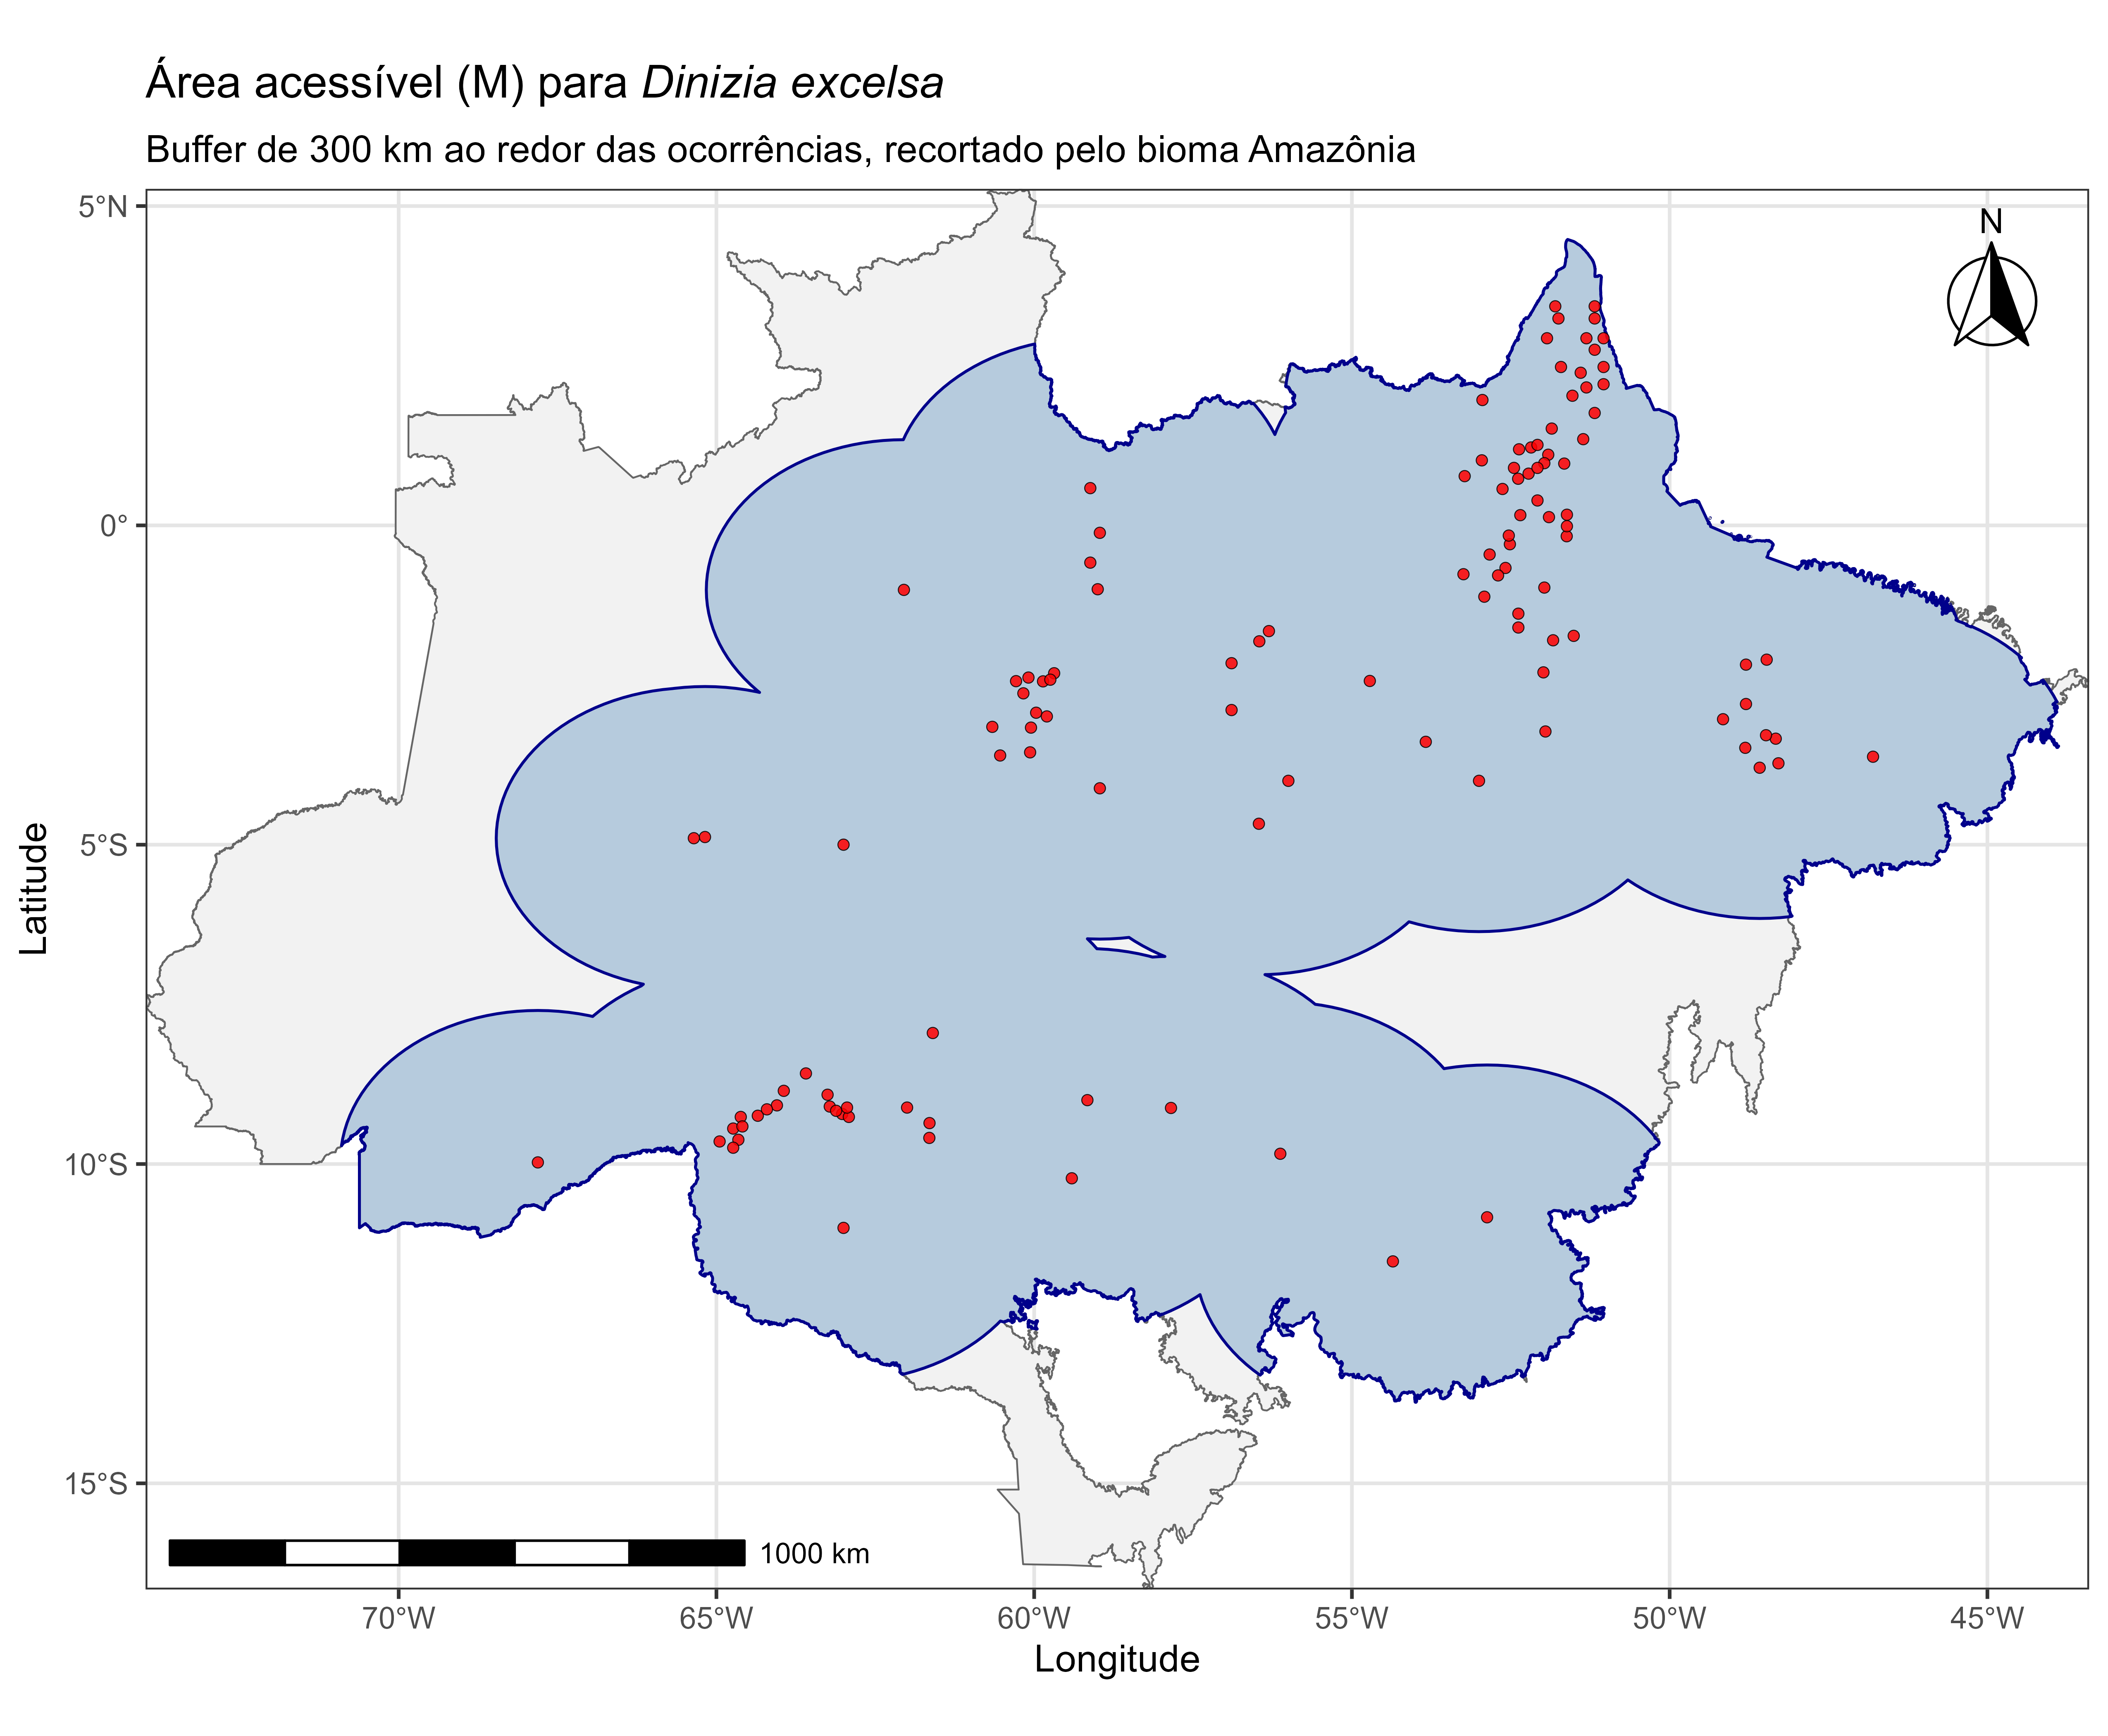
\includegraphics[width=0.90\textwidth]{figuras/unidade05/unidade05_area_m_dinizia.png}
  \caption{Accessible area ($M$) delineated for \textit{Dinizia excelsa} within the Amazon biome. The area was defined by buffering occurrences and cropping the result to the biome boundary.}
  \label{fig:unidade05_area_m_dinizia}
\end{figure}

\section{Background Selection}

Background points represent the environment available during model calibration.
They are not confirmed absences. They characterize environmental conditions
available within the area considered accessible.

\rscriptfile{scripts/unidade05/03_gerar_background_area_m.R}

\begin{figure}[H]
  \centering
  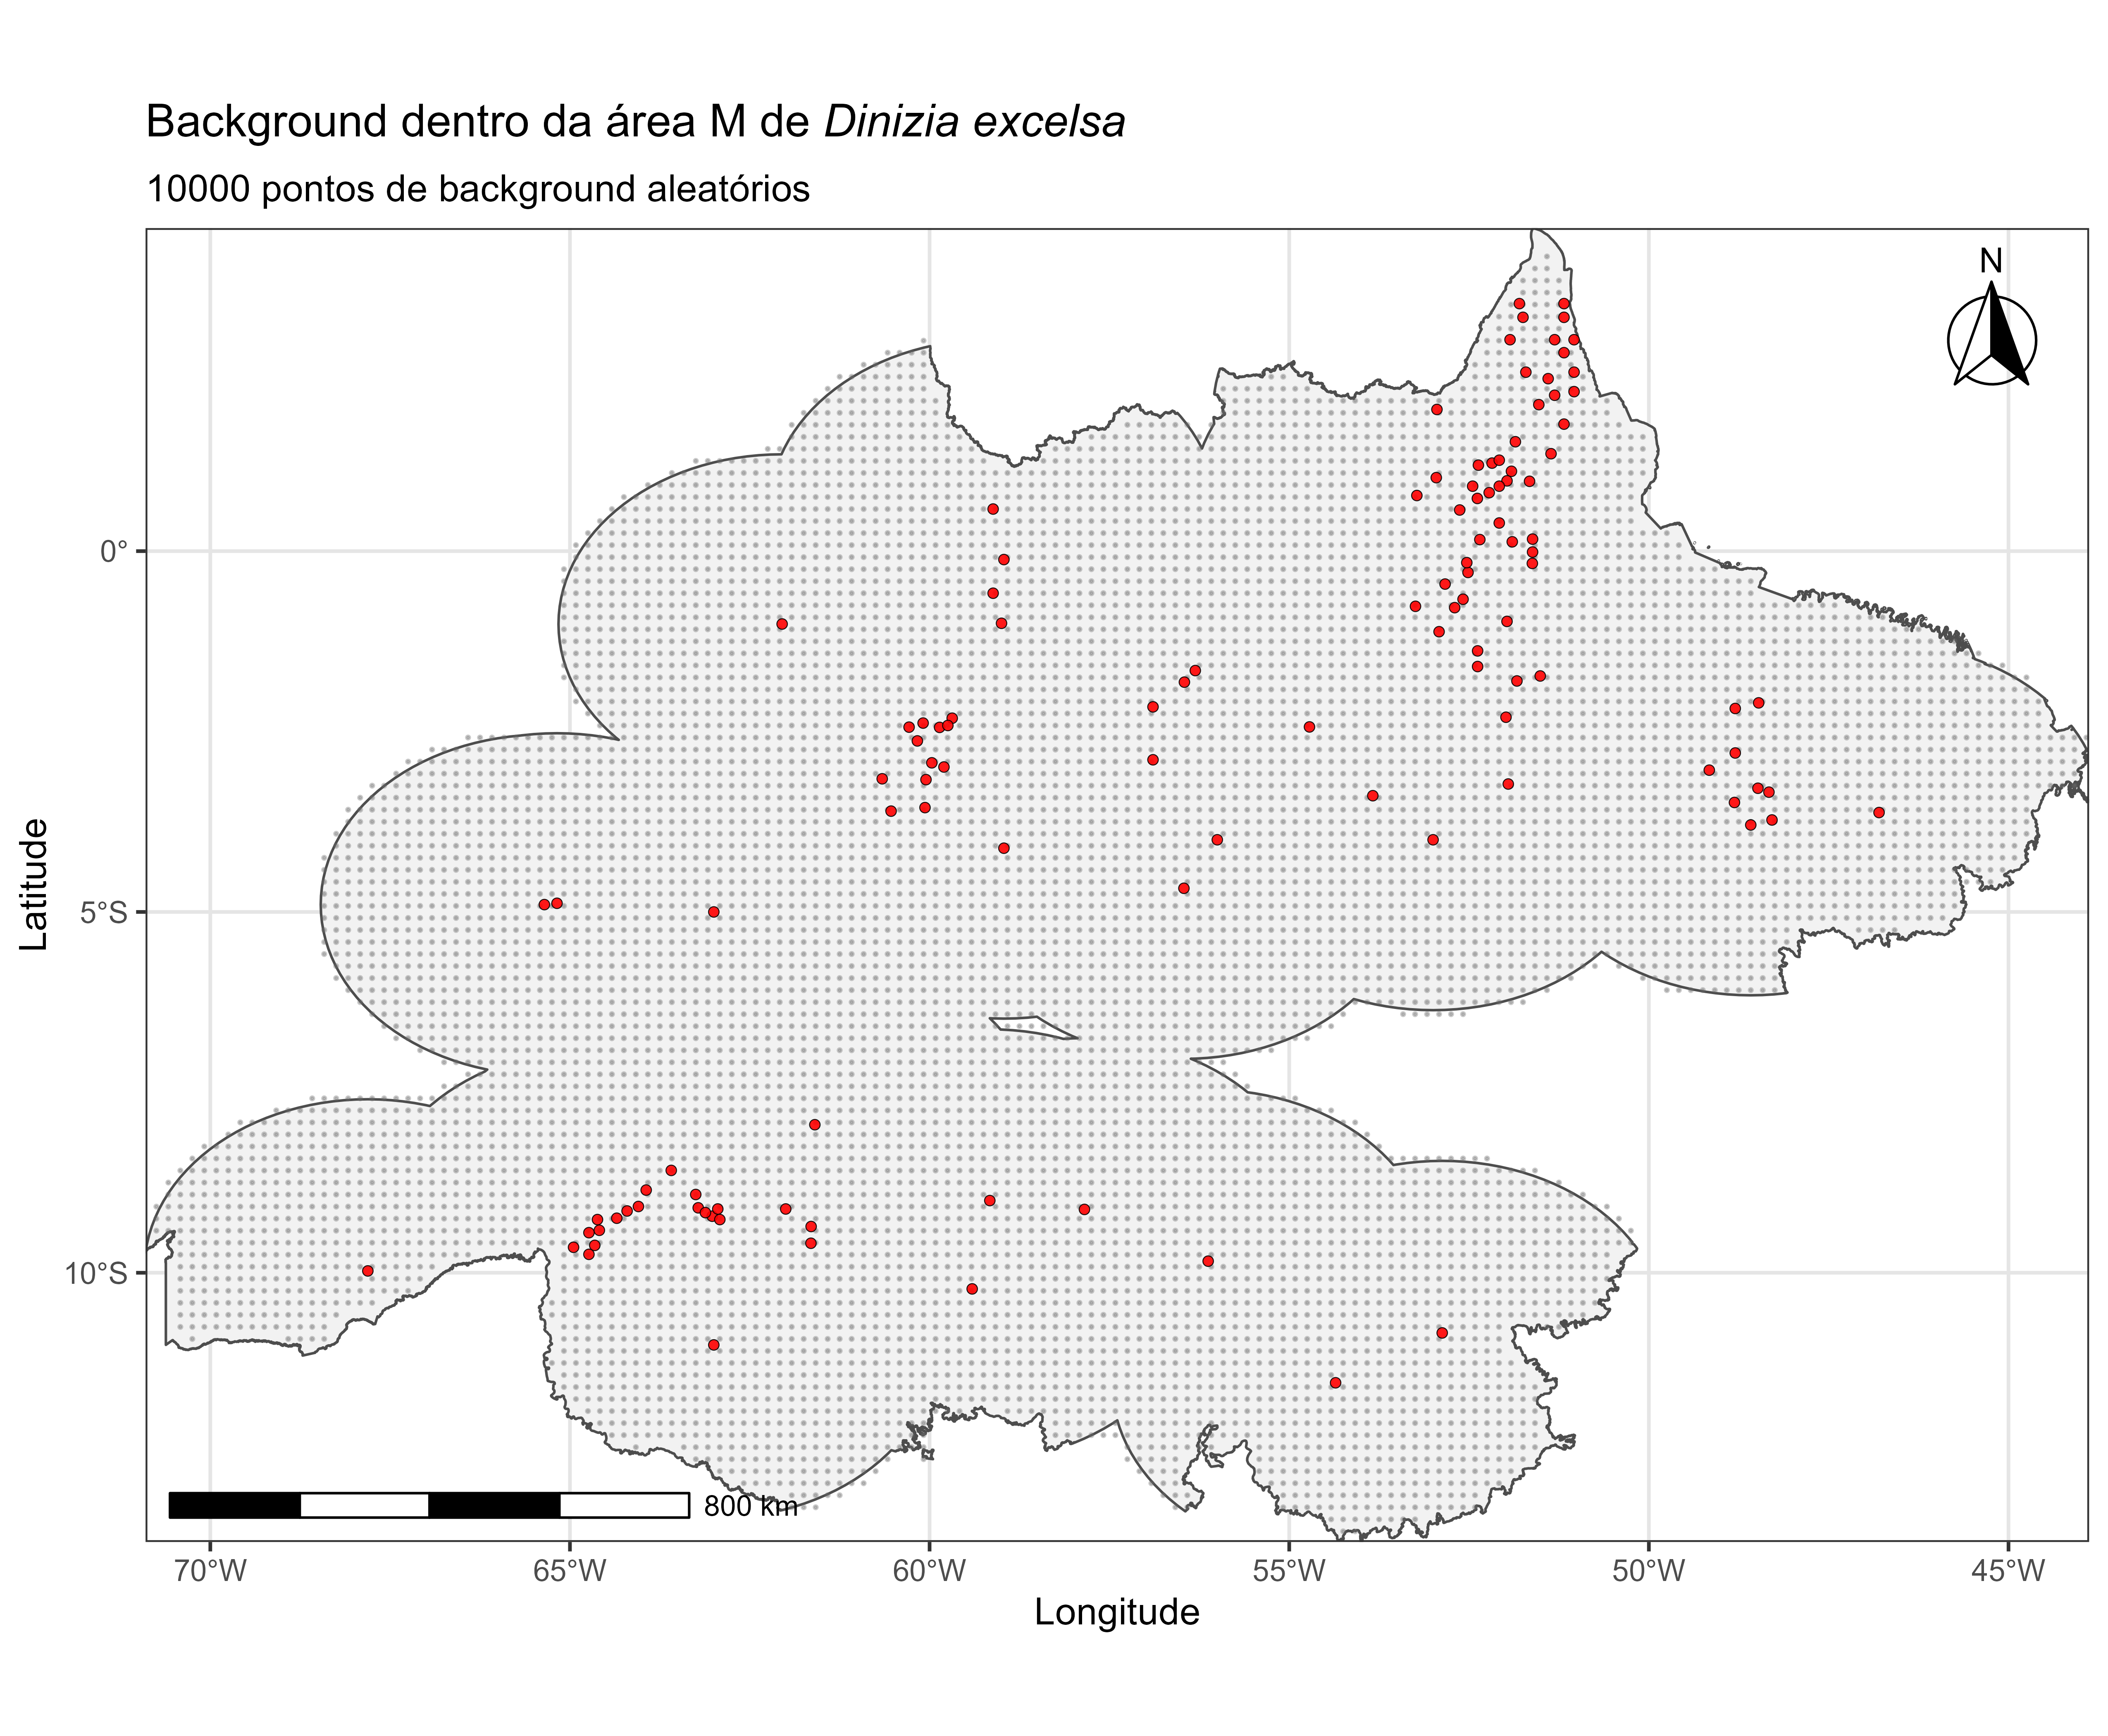
\includegraphics[width=0.90\textwidth]{figuras/unidade05/unidade05_background_area_m.png}
  \caption{Background points sampled within the accessible area ($M$) of \textit{Dinizia excelsa}.}
  \label{fig:unidade05_background_m}
\end{figure}

\section{Biome-Wide Background versus Background within M}

Background selection can substantially change the environmental distribution
available to a model. It is therefore informative to compare samples from the
entire biome with samples restricted to $M$.

\rscriptfile{scripts/unidade05/04_comparar_background_bioma_m.R}

\begin{figure}[H]
  \centering
  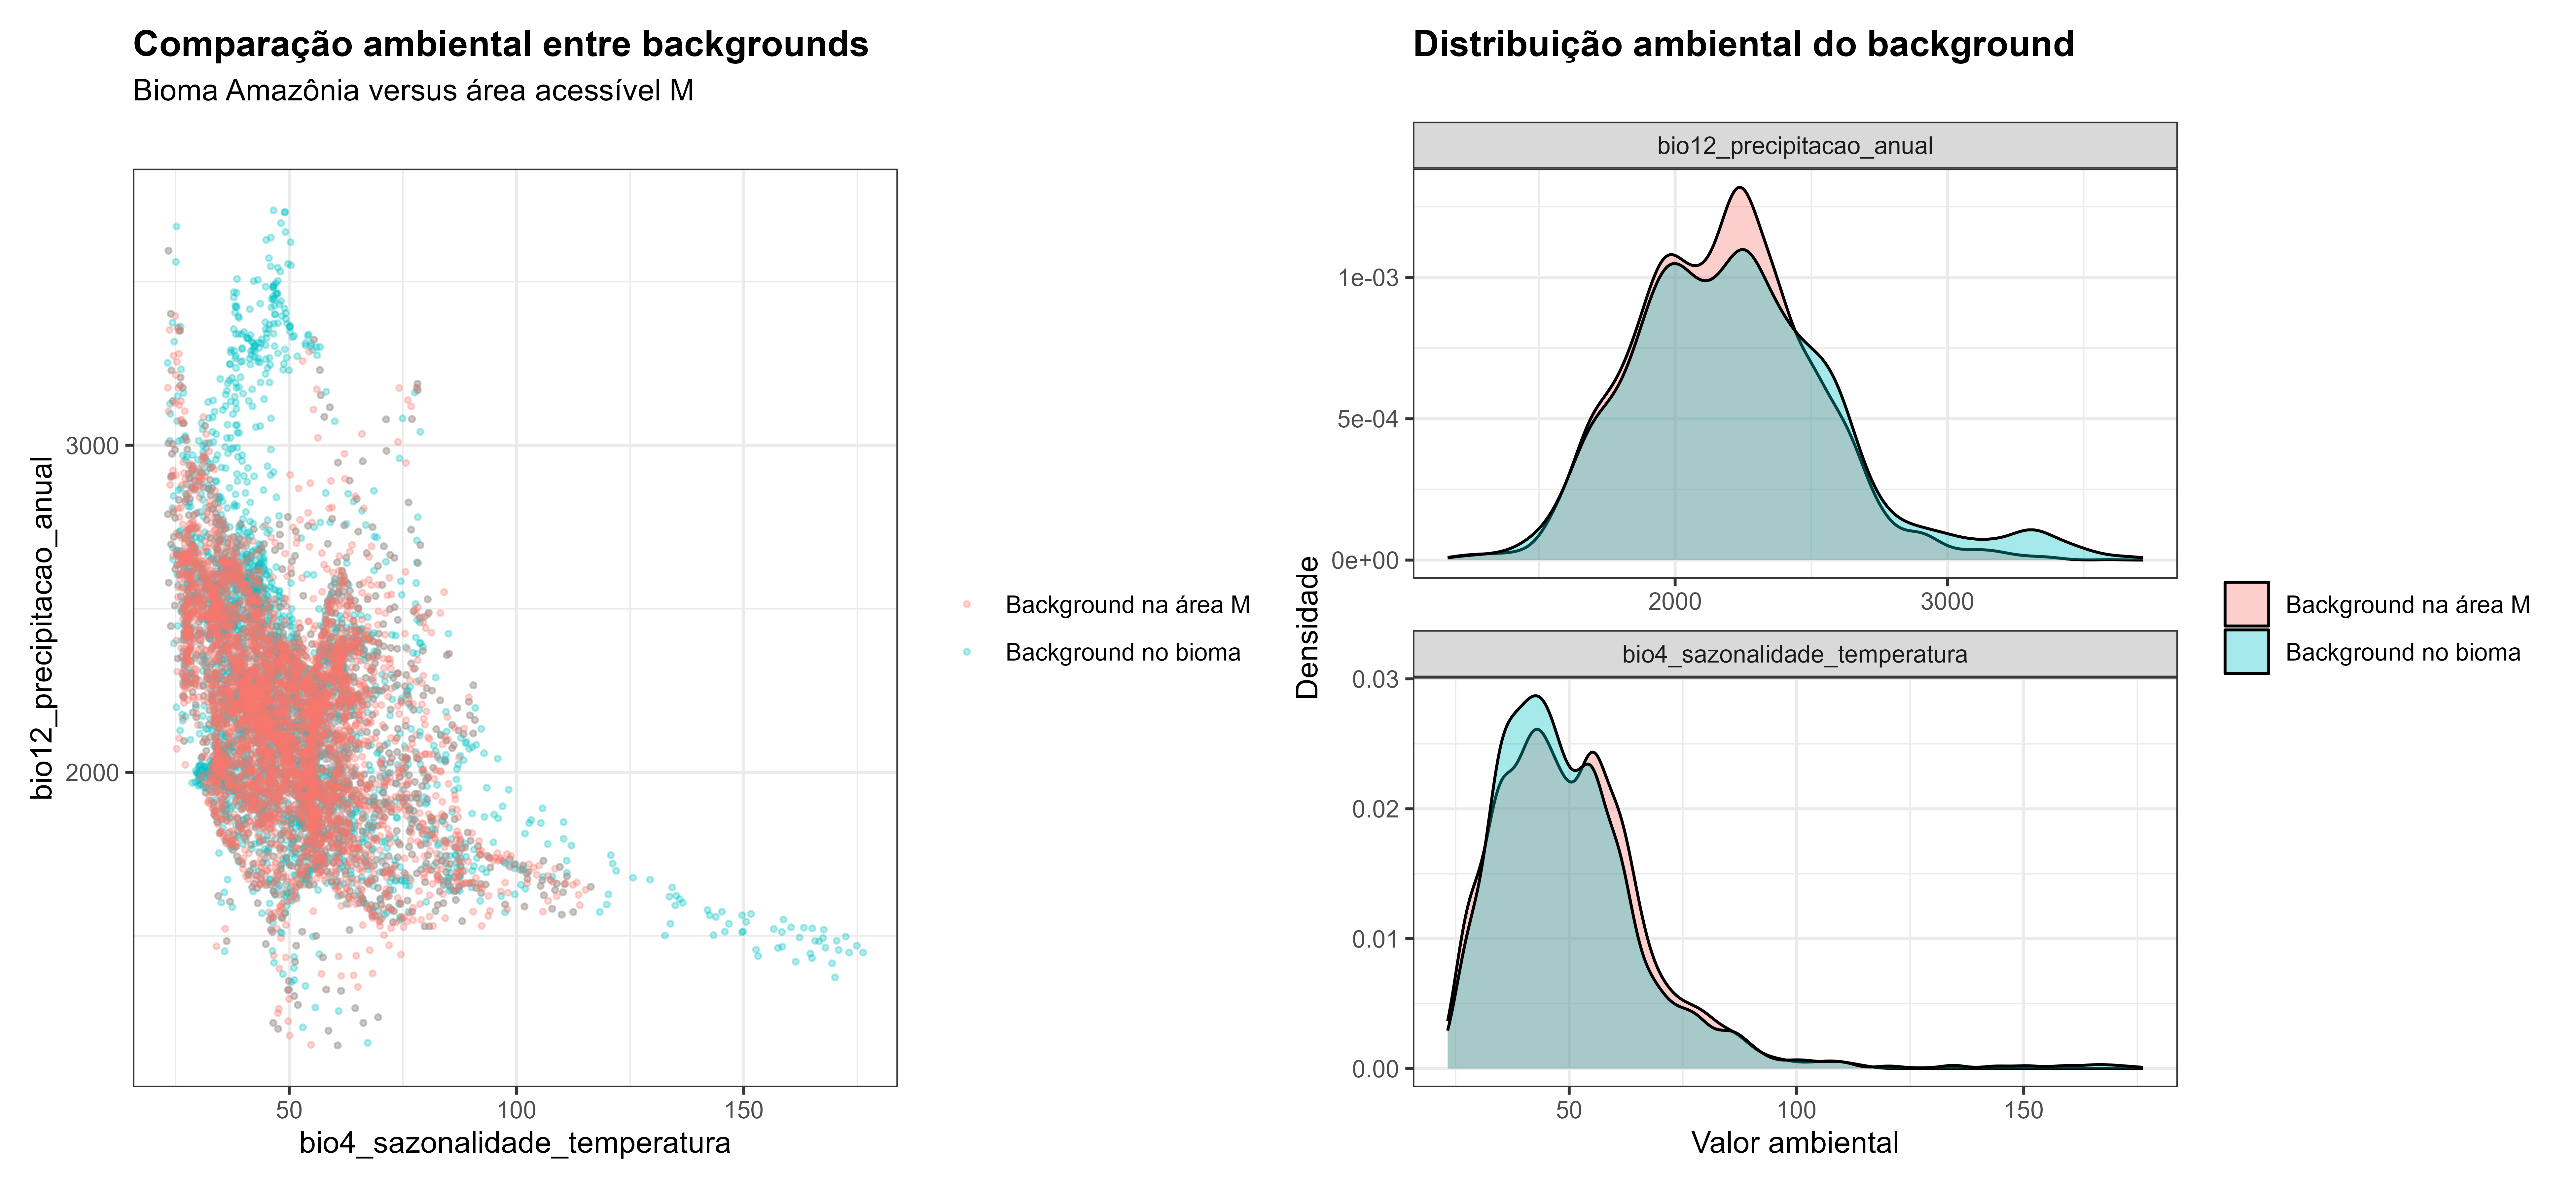
\includegraphics[width=0.90\textwidth]{figuras/unidade05/unidade05_comparacao_background.png}
  \caption{Comparison between background sampled throughout the Amazon biome and background restricted to the accessible area ($M$).}
  \label{fig:unidade05_comparacao_background}
\end{figure}

\section{Environmental Extraction and the Presence--Background Dataset}

The selected environmental variables are extracted at the presences and at
background points within $M$, producing the presence--background dataset used
in subsequent chapters.

\rscriptfile{scripts/unidade05/05_preparar_presenca_background.R}

\begin{figure}[H]
  \centering
  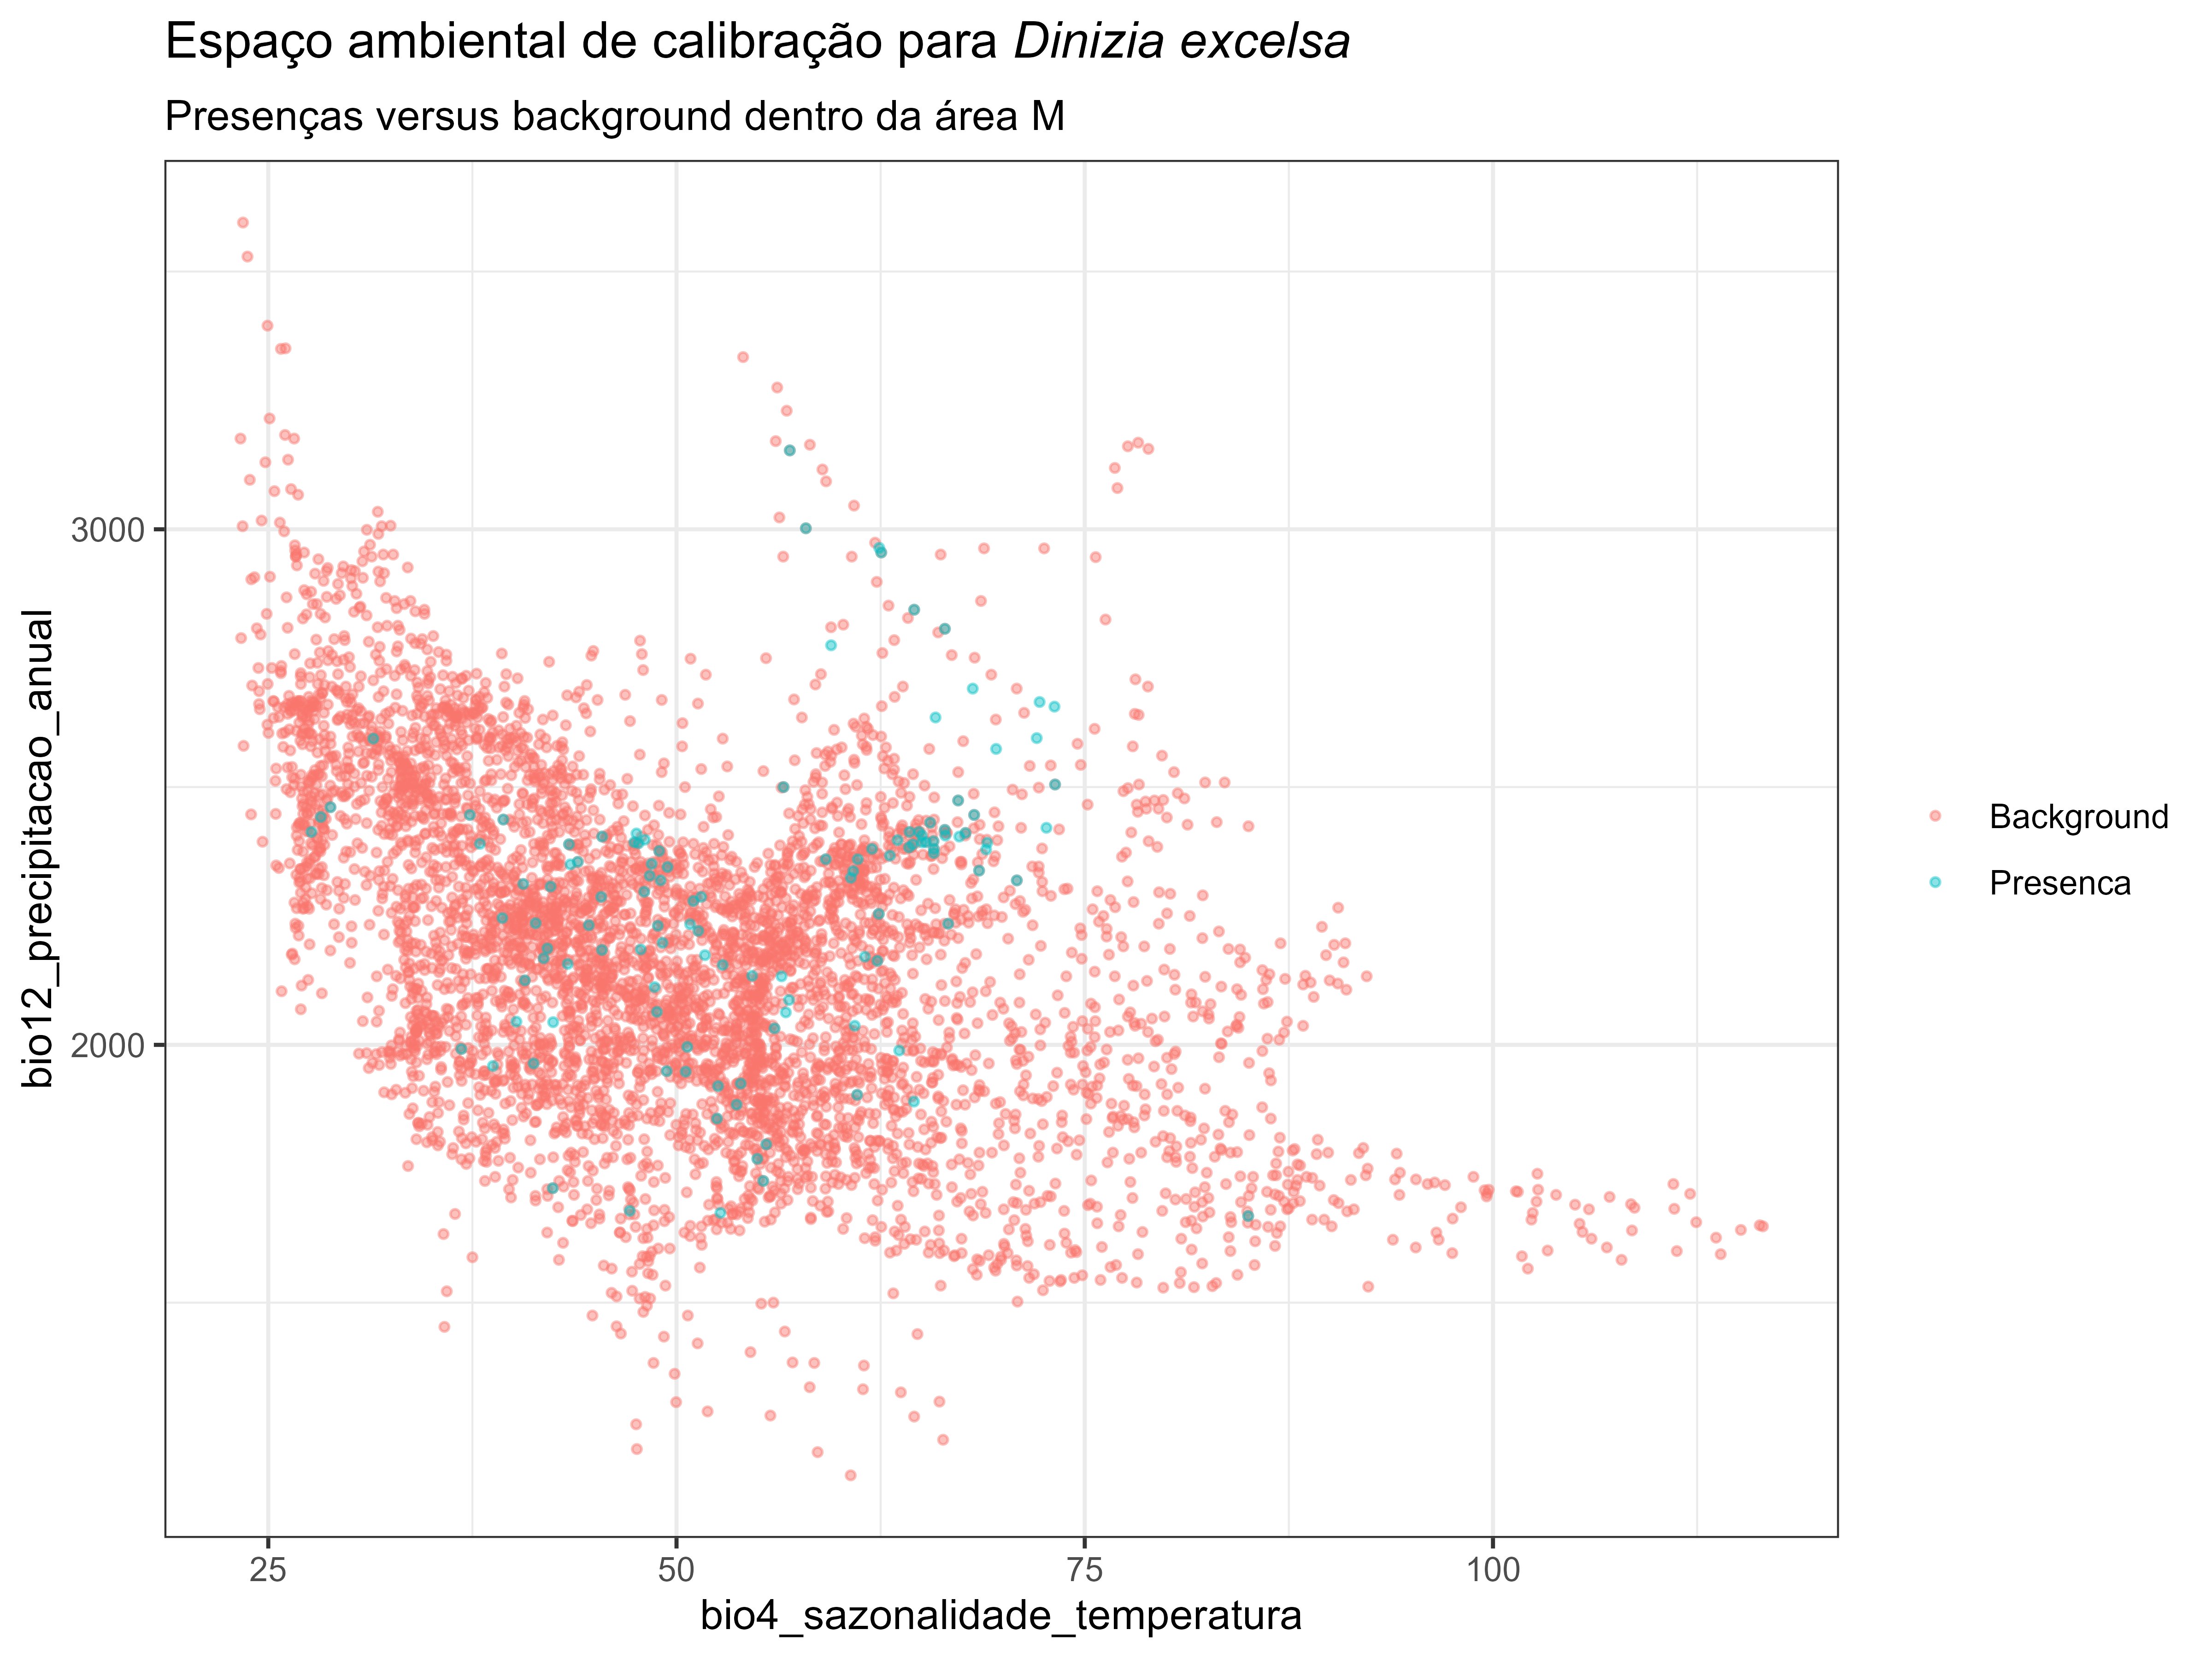
\includegraphics[width=0.86\textwidth]{figuras/unidade05/unidade05_espaco_ambiental_presenca_background.png}
  \caption{Environmental-space comparison between \textit{Dinizia excelsa} presences and background within the accessible area ($M$).}
  \label{fig:unidade05_espaco_presenca_background}
\end{figure}

\section{Complete Pipeline}
\rscriptfile{scripts/unidade05/06_pipeline_area_m_background.R}

\section{Chapter Summary}

Defining $M$ is an ecological, biogeographic, and methodological decision. It
affects model background, calibration, evaluation, and projection. The
operational $M$ delineated for \textit{Dinizia excelsa} provides a coherent
foundation for the models developed in the following chapters.

\begin{conceito}[title={\faBook\quad Key message}]
Background should represent the environment available to a species within its
accessible area. A model calibrated with inappropriate background can yield
biologically fragile maps even when statistical metrics appear strong.
\end{conceito}


\chapter[GLM]{Generalized Linear Models}

\begin{objetivos}
By the end of this chapter, readers should understand generalized linear models
(GLMs) in SDM; fit presence--background models with a binomial family;
interpret coefficients and linear and quadratic terms; assess predictive
performance using AUC and TSS; generate partial response curves; project
environmental suitability into geographic space; and map current suitability
for \textit{Dinizia excelsa} across the Amazon biome.
\end{objetivos}

\section{Introduction}

Generalized linear models are among the most established and interpretable
statistical approaches in species distribution modeling. They commonly relate
presence--absence or presence--background observations to environmental
predictors \parencite{guisan2000,guisan2005predicting,guisan2017habitat}.

In a presence--background model, presences are coded 1 and background points 0.
Background points are not confirmed absences; they represent the environmental
conditions available within the calibration area. With background coded as the
contrast class, the fitted GLM estimates a relative occurrence or environmental
suitability score along the environmental gradients, not an absolute occurrence
probability.

\begin{conceito}[title={\faBook\quad GLMs in SDM}]
A binomial GLM uses a logit link to relate species occurrence to environmental
variables, transforming a linear predictor into values between 0 and 1.
\end{conceito}

\section{Mathematical Formulation}

For the binomial case, let $Y_i$ indicate presence or background:

\[
Y_i =
\begin{cases}
  1, & \text{presence},\\
  0, & \text{background}.
\end{cases}
\]

The GLM with a logit link is

\begin{equationbox}
\[
\operatorname{logit}(p_i)=
\log\left(\frac{p_i}{1-p_i}\right)
=\beta_0+\beta_1X_{1i}+\beta_2X_{2i}+\cdots+\beta_kX_{ki},
\]
\[
p_i=\frac{1}{1+\exp(-\eta_i)}.
\]
\end{equationbox}

Here, $p_i$ is estimated suitability in pixel $i$, $X_k$ denotes the
environmental predictors, and $\beta_k$ denotes estimated coefficients.

\begin{dica}[title={\faLightbulb\quad Quadratic terms}]
Quadratic terms allow unimodal responses in which suitability is greatest at
intermediate values of an environmental variable.
\end{dica}

\section{Preparing Data for the GLM}

The presence--background dataset from Chapter 5 is used here. Presences are the
final \textit{Dinizia excelsa} records, and background points were sampled
within the accessible area $M$. Together they form the calibration dataset.

\rscriptfile{scripts/unidade06/01_estrutura_pastas.R}
\rscriptfile{scripts/unidade06/02_preparar_dados_glm.R}

\section{Fitting the GLM}

The model uses a binomial family and logit link. Linear and quadratic terms
increase ecological flexibility. Before fitting, predictors are standardized
to zero mean and unit standard deviation, reducing numerical problems and
facilitating coefficient comparisons.

\rscriptfile{scripts/unidade06/03_ajustar_glm_dinizia.R}

\begin{figure}[H]
  \centering
  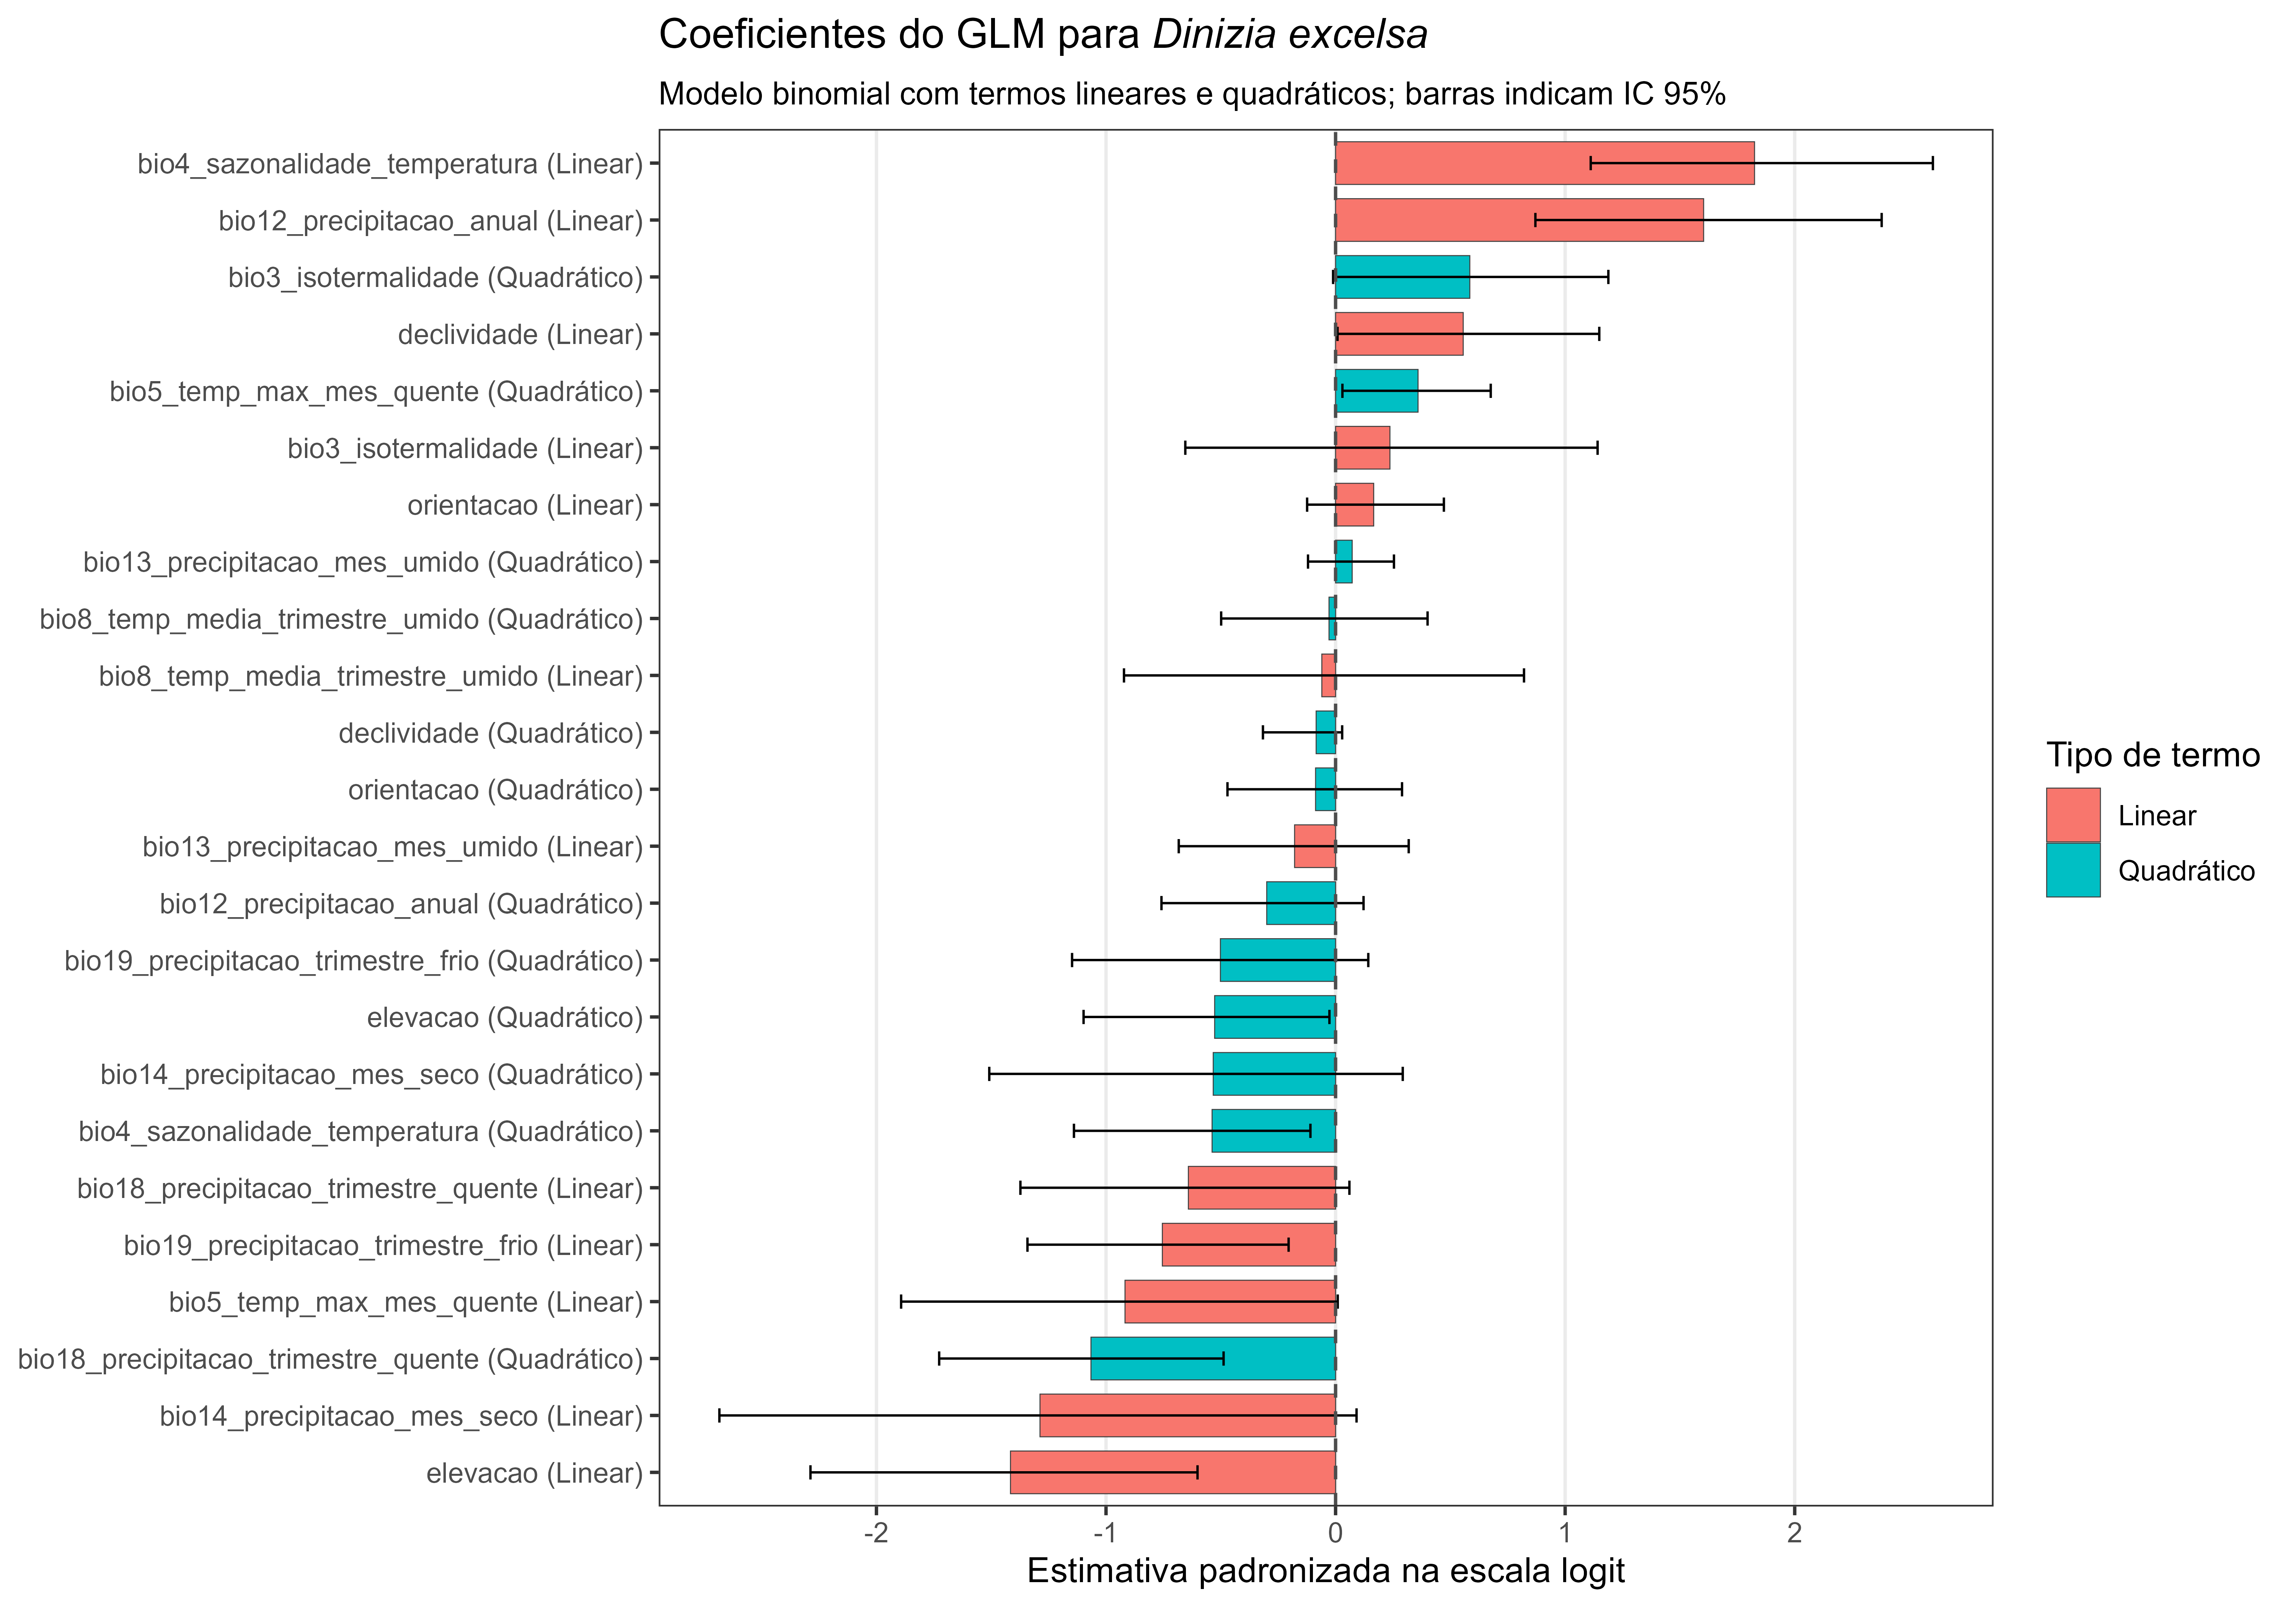
\includegraphics[width=0.88\textwidth]{figuras/unidade06/unidade06_coeficientes_glm.png}
  \caption{GLM coefficients estimated for \textit{Dinizia excelsa}. Conditional on the other model terms, positive values indicate positive associations with relative suitability and negative values indicate negative associations.}
  \label{fig:unidade06_coeficientes_glm}
\end{figure}

\section{Model Evaluation}

The GLM is evaluated using AUC, TSS, sensitivity, specificity, and a confusion
matrix. AUC summarizes discrimination across thresholds; TSS combines
sensitivity and specificity. With presence--background data, these metrics are
comparative indicators rather than absolute validation of the species' actual
distribution.

\rscriptfile{scripts/unidade06/04_avaliar_glm_dinizia.R}

\begin{figure}[H]
  \centering
  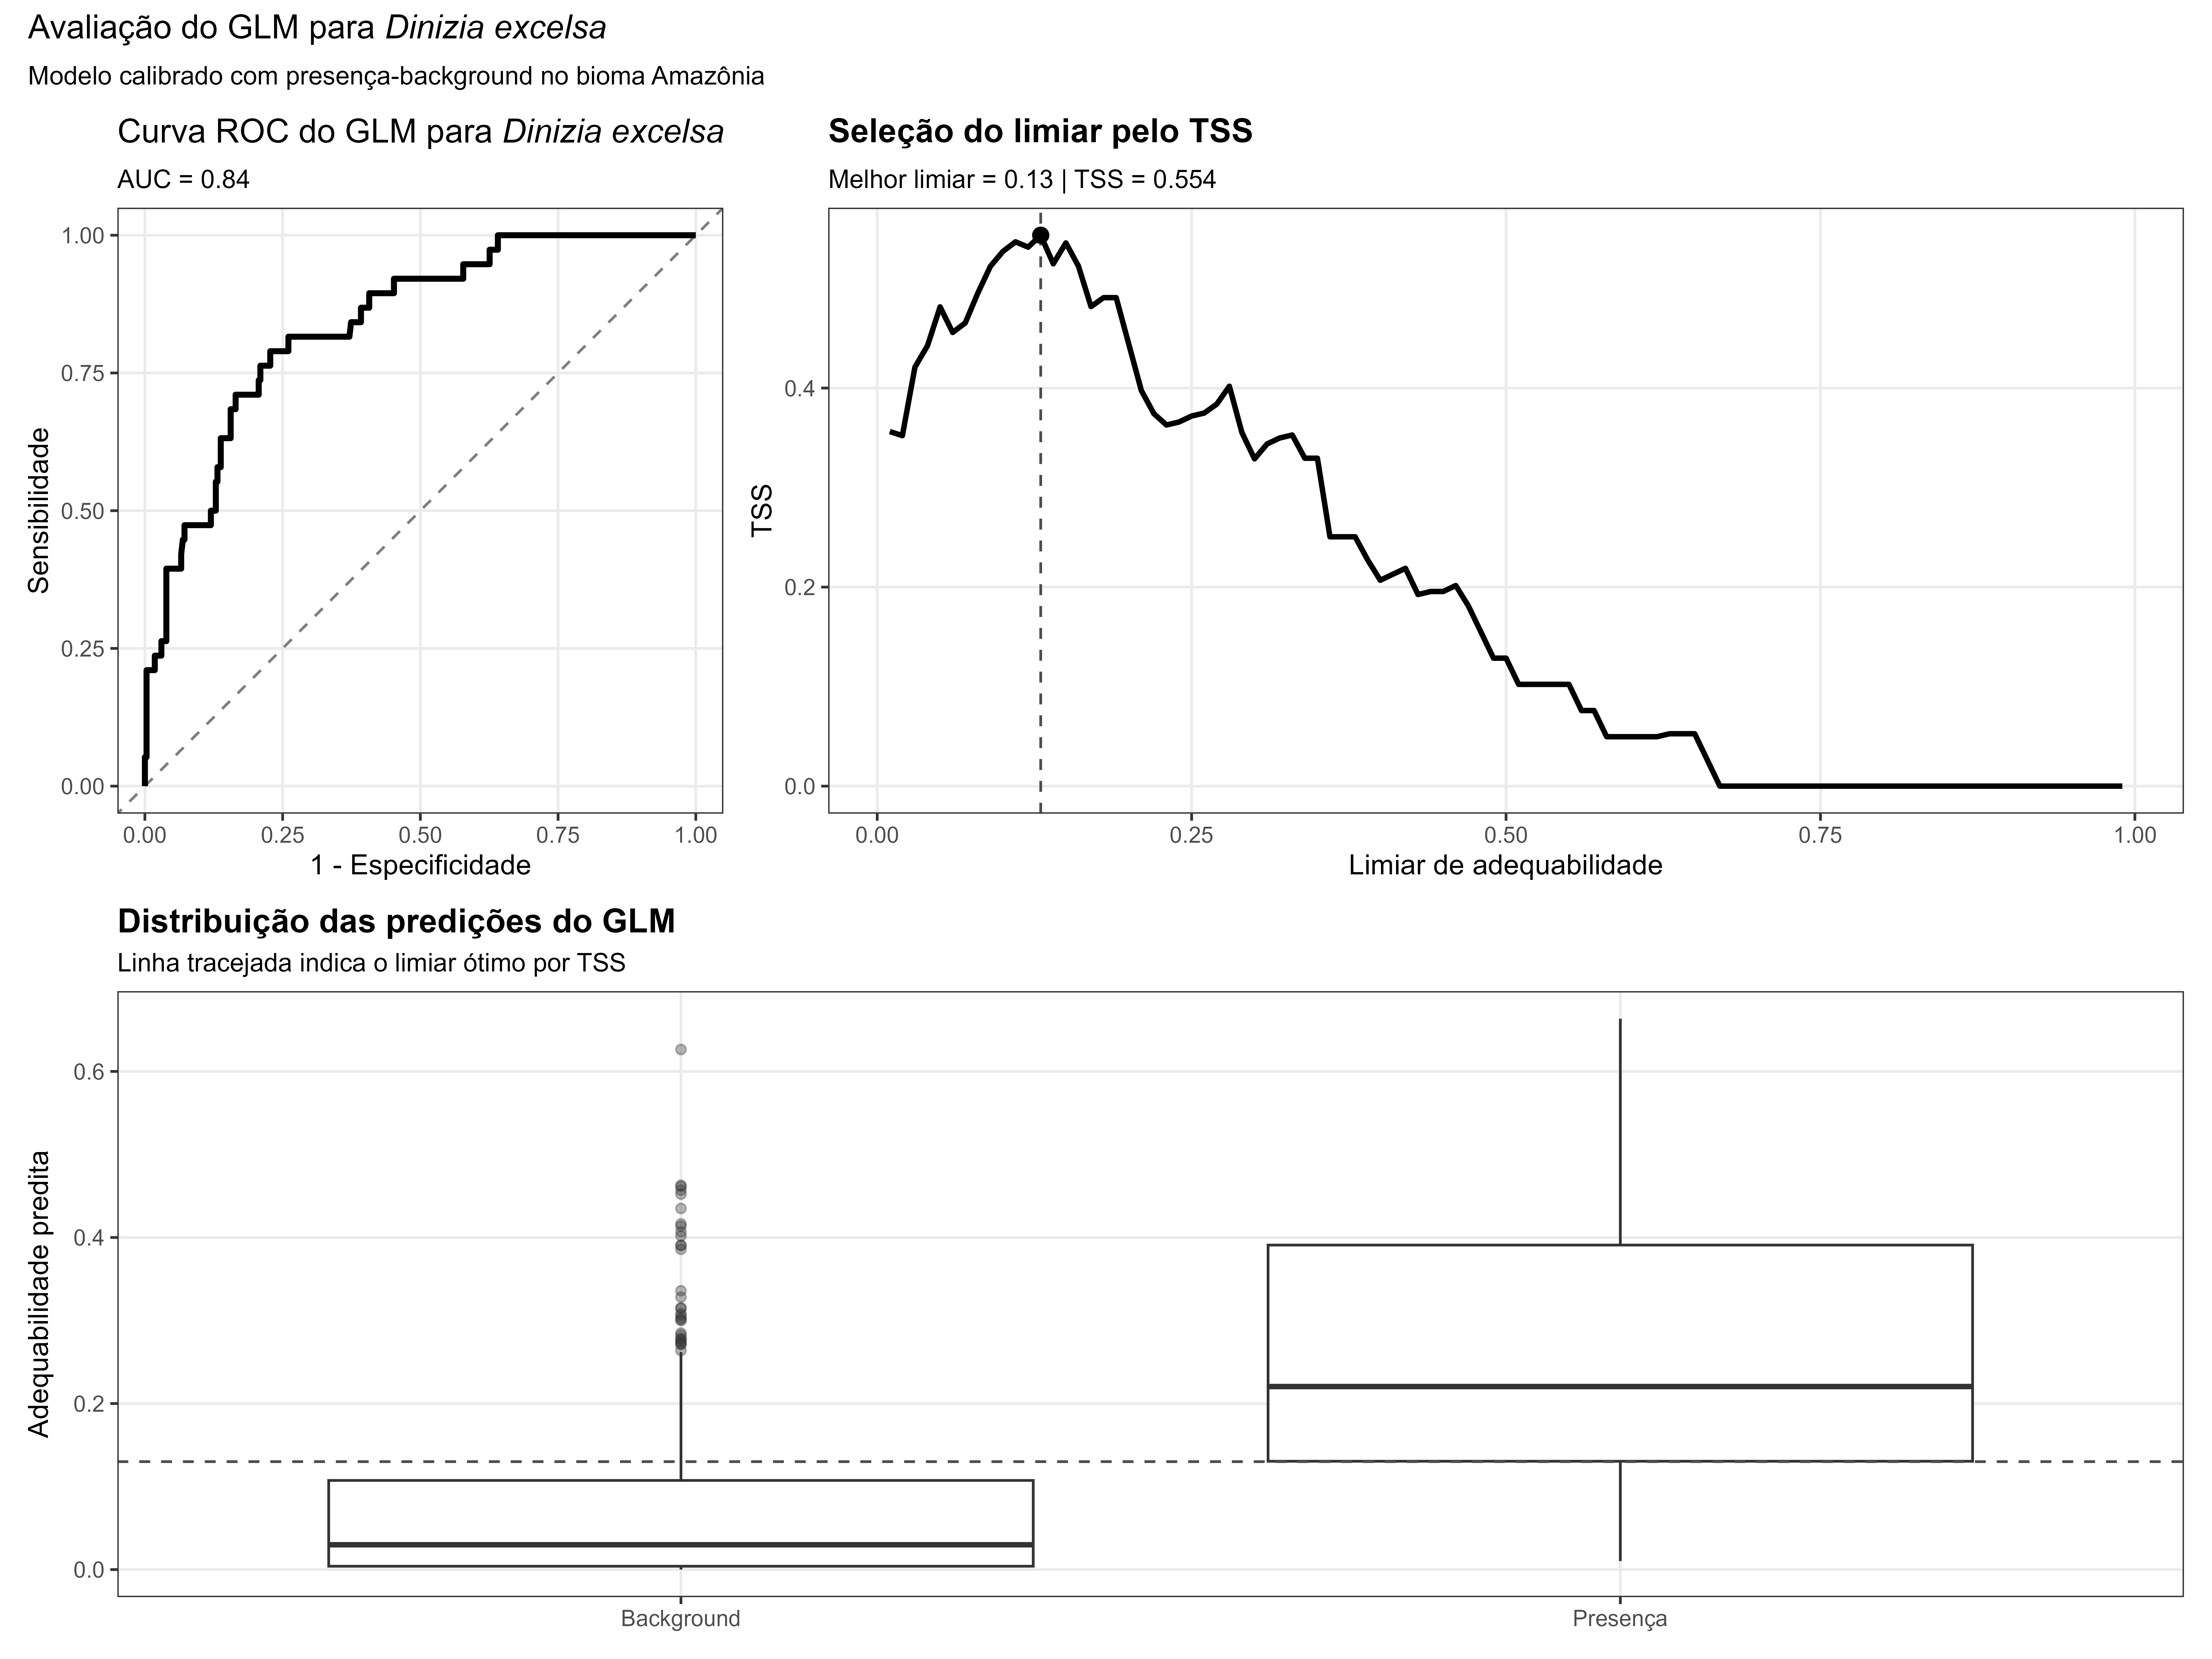
\includegraphics[width=0.82\textwidth]{figuras/unidade06/unidade06_avaliacao_glm_patchwork.png}
  \caption{ROC curve for the GLM fitted to \textit{Dinizia excelsa}.}
  \label{fig:unidade06_roc_glm}
\end{figure}

\section{Partial Response Curves}

Partial response curves show how estimated suitability changes along one
predictor while the others are held constant. They are essential for ecological
interpretation of model behavior.

\rscriptfile{scripts/unidade06/06_curvas_resposta_glm.R}

\begin{figure}[H]
  \centering
  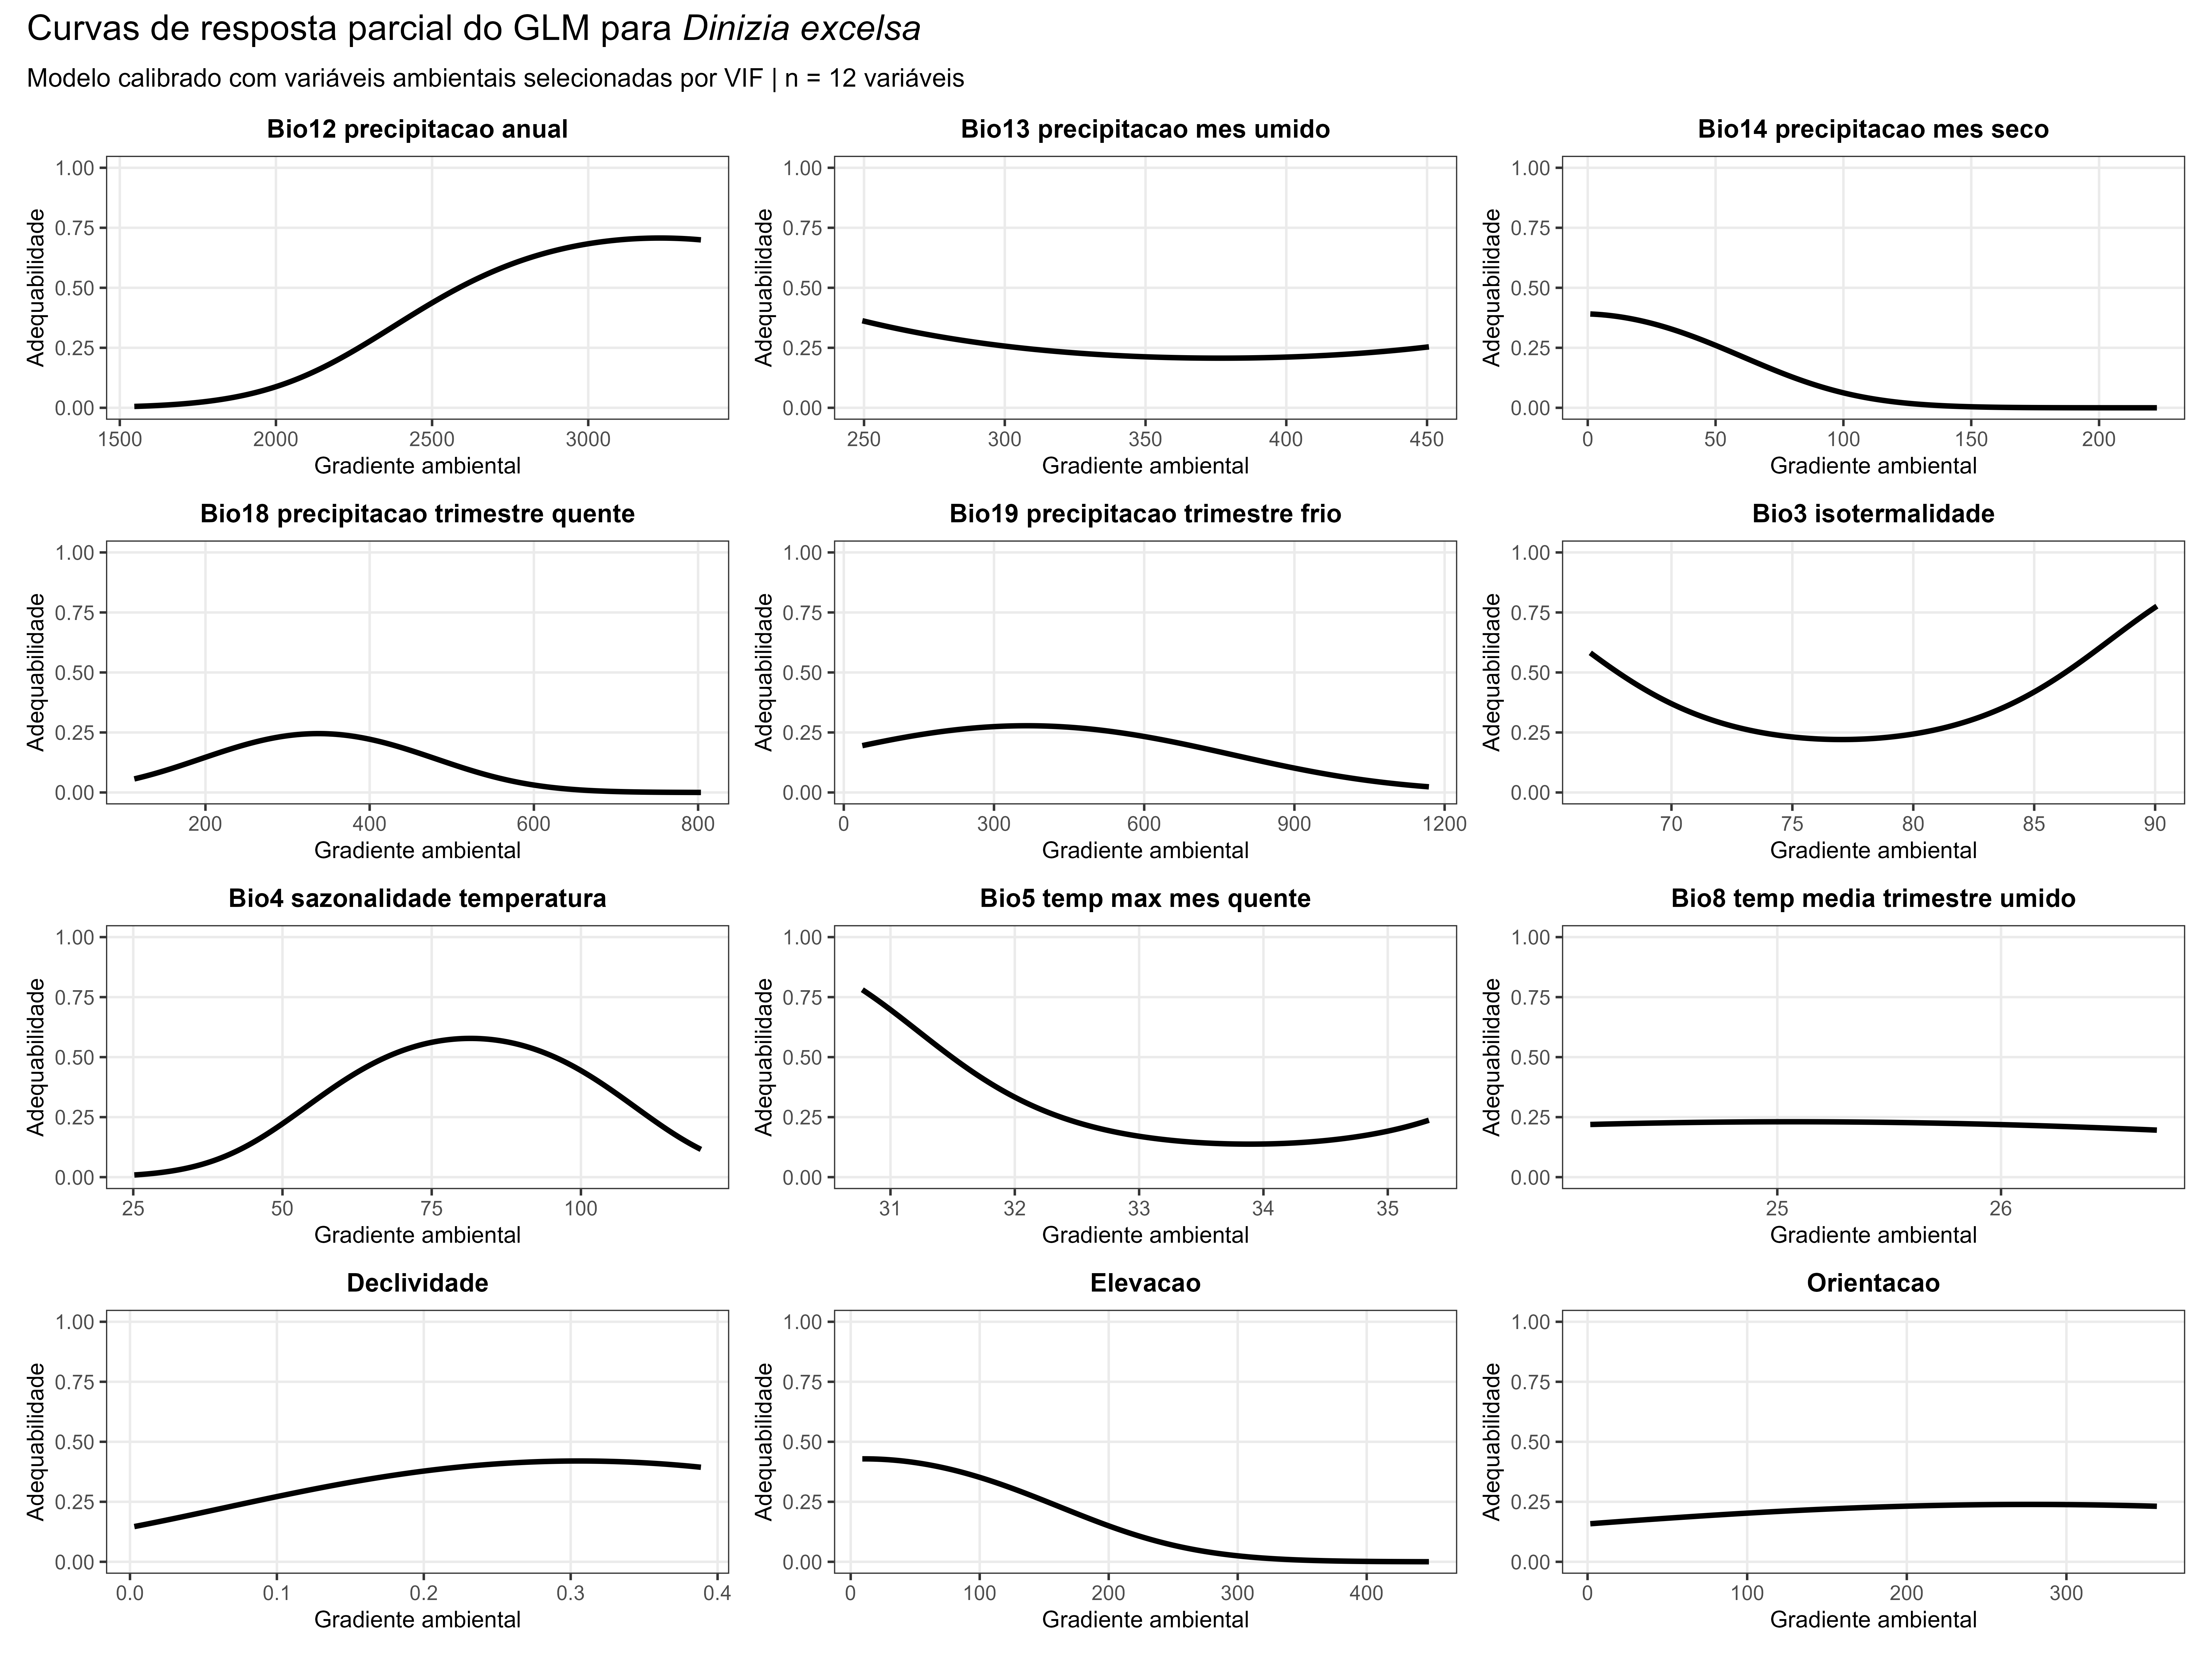
\includegraphics[width=0.96\textwidth]{figuras/unidade06/unidade06_curvas_resposta_glm.png}
  \caption{Partial response curves from the GLM for the selected environmental predictors.}
  \label{fig:unidade06_curvas_resposta}
\end{figure}

\section{Spatial Projection of Current Suitability}

After fitting and evaluation, the GLM is projected onto the environmental stack
for the study area, producing a continuous map of current environmental
suitability for \textit{Dinizia excelsa}.

\rscriptfile{scripts/unidade06/05_predicao_espacial_glm.R}

\begin{figure}[H]
  \centering
  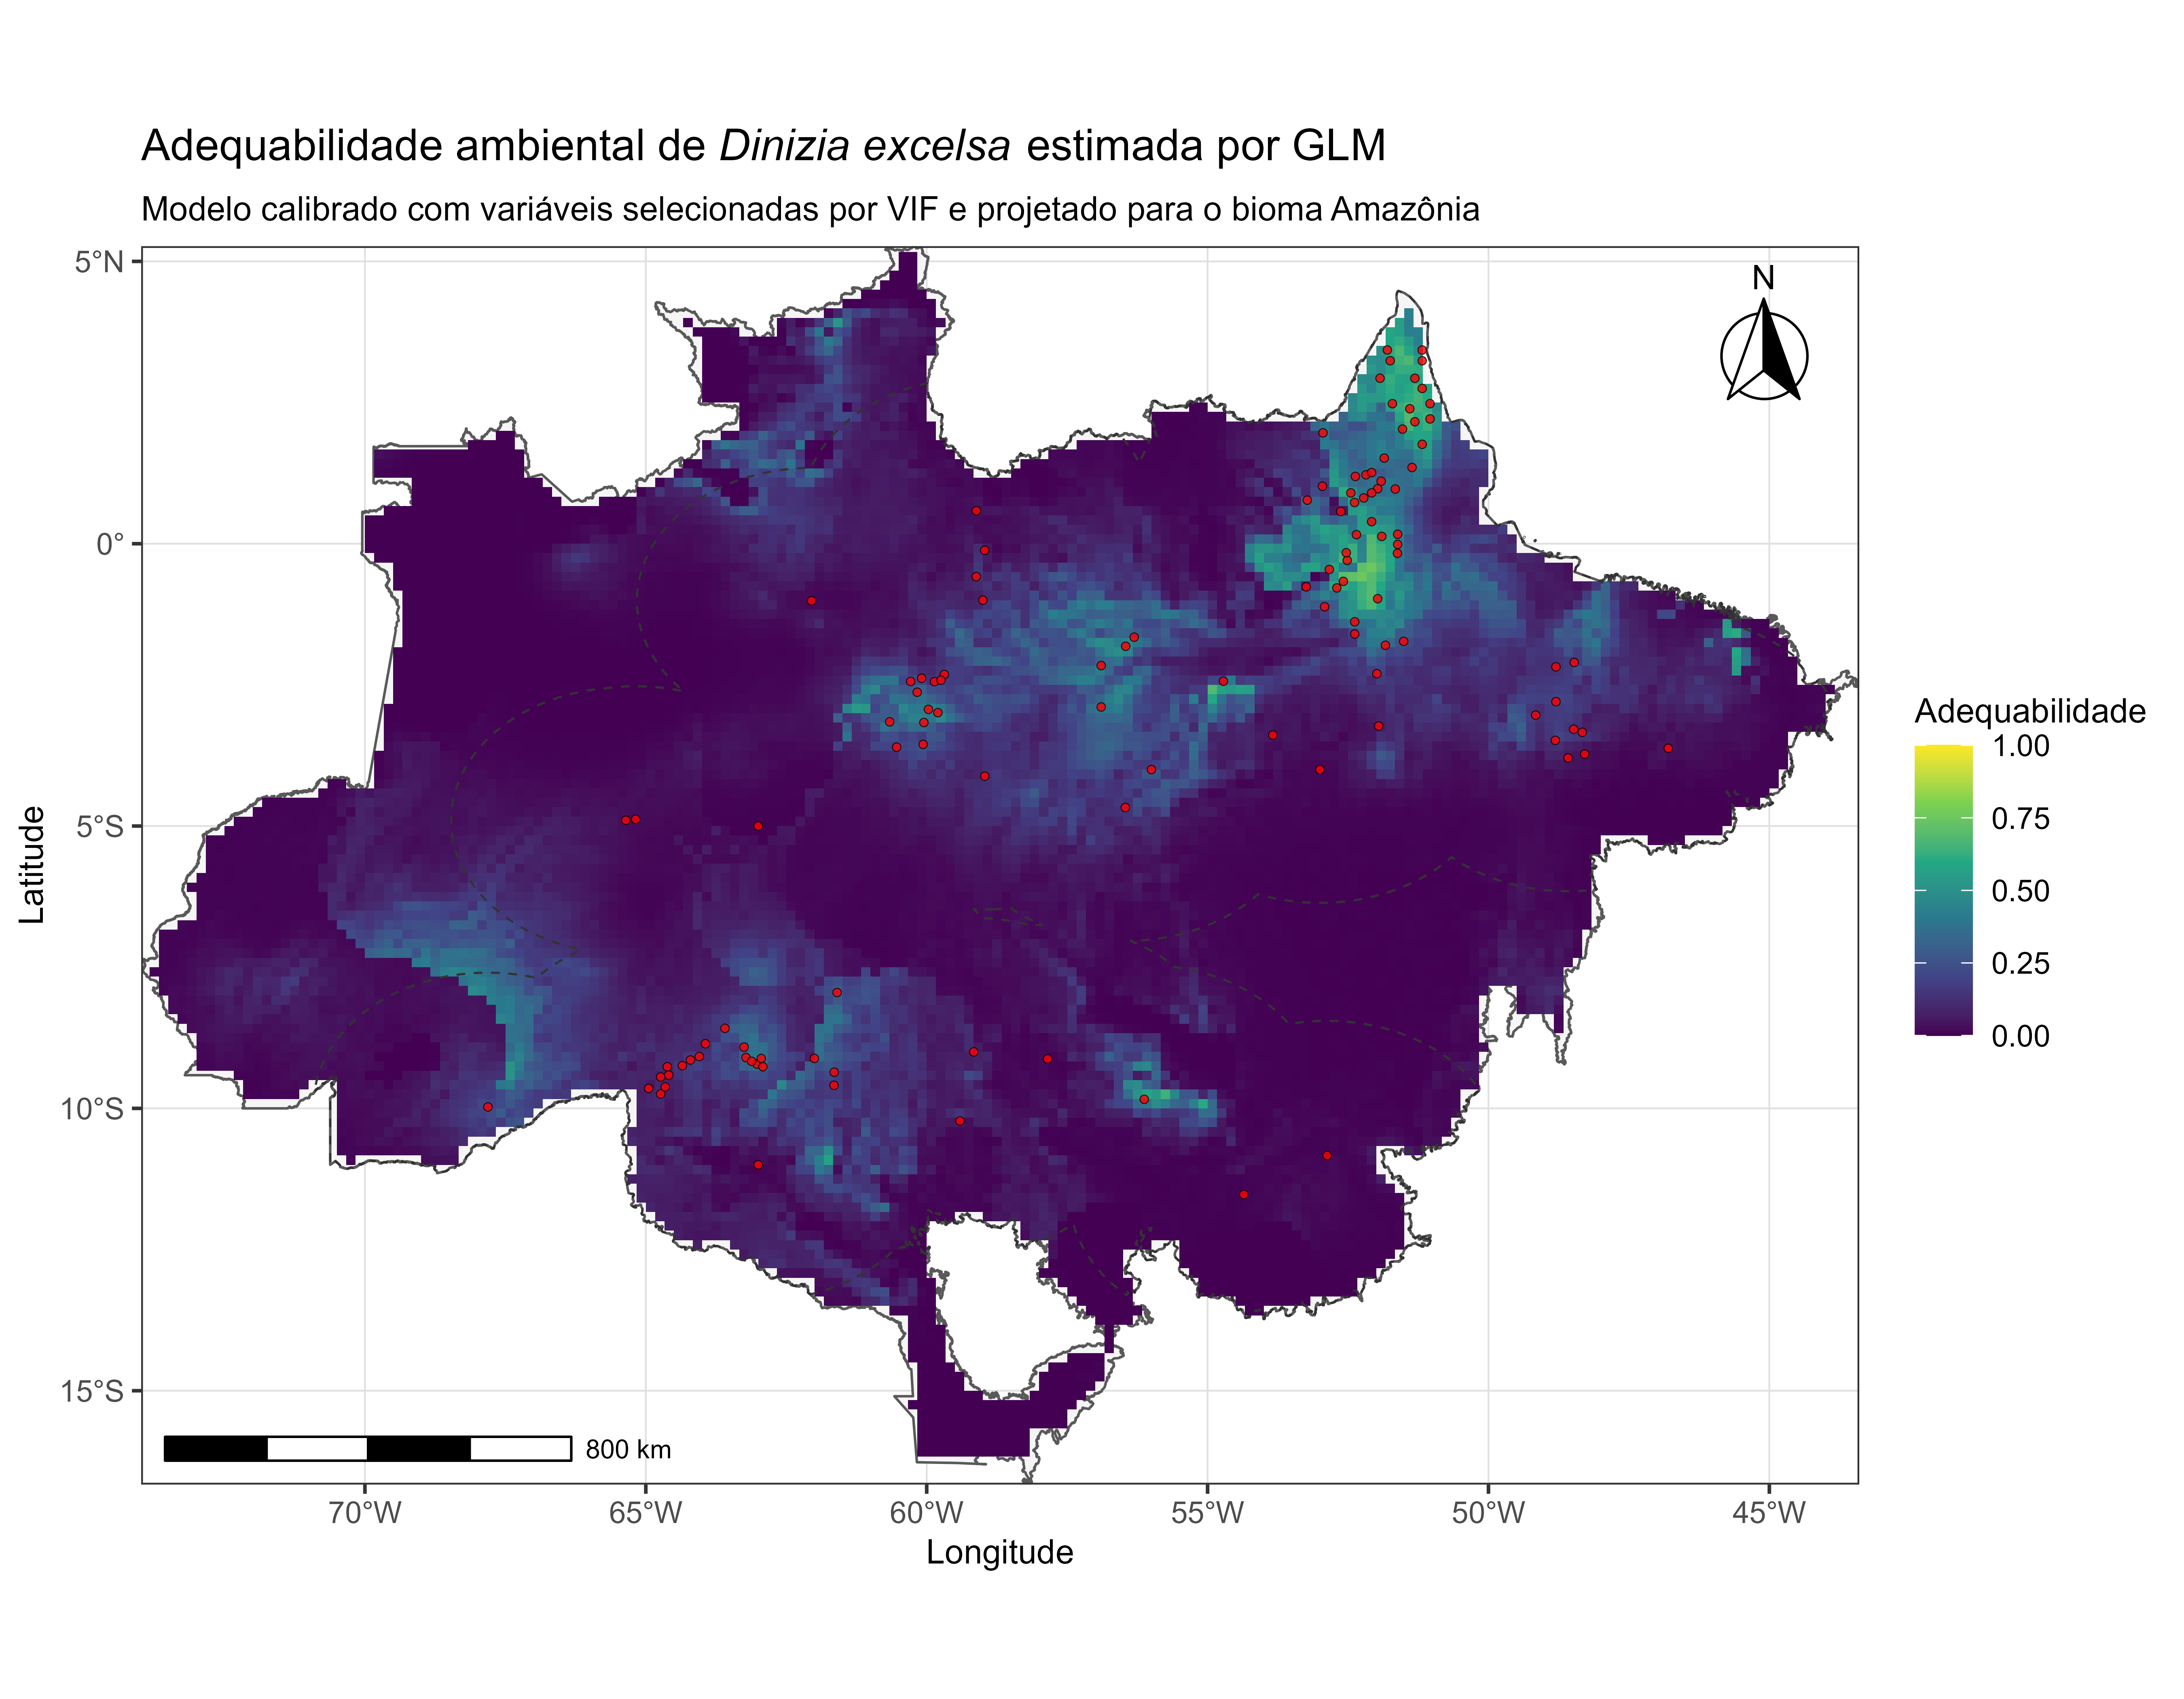
\includegraphics[width=0.90\textwidth]{figuras/unidade06/unidade06_adequabilidade_glm.png}
  \caption{Current environmental suitability for \textit{Dinizia excelsa} estimated with a GLM.}
  \label{fig:unidade06_adequabilidade_glm}
\end{figure}

\section{Complete Pipeline}
\rscriptfile{scripts/unidade06/07_pipeline_glm.R}

\section{Chapter Summary}

The GLM is a simple, interpretable, and robust starting point for SDM. Although
less flexible than GAM, Random Forest, BRT, or Maxent, it makes the relationship
between occurrence and environmental gradients explicit. It is consequently
valuable in teaching, exploratory analysis, and studies prioritizing
transparency and ecological interpretation.

\begin{conceito}[title={\faBook\quad Key message}]
The GLM bridges classical statistics and modern SDM: it is simple enough for
ecological interpretation but sufficiently powerful to produce suitability
maps when calibrated appropriately.
\end{conceito}

\section{Review Exercises}
\begin{enumerate}
  \item Why is the binomial family appropriate for presence--background models?
  \item What does the logit function represent in a GLM?
  \item Why are quadratic terms useful in SDM?
  \item Distinguish positive and negative GLM coefficients.
  \item Explain the difference between AUC and TSS.
  \item Why are partial response curves important for ecological interpretation?
  \item Which limitations should be considered when using GLMs for spatial projection?
\end{enumerate}

\chapter[GAM]{Generalized Additive Models}

\begin{objetivos}
By the end of this chapter, readers should understand generalized additive
models (GAMs) in SDM; fit presence--background models with smooth terms;
interpret smooth functions; evaluate discrimination using AUC, TSS,
sensitivity, and specificity; generate partial response curves and suitability
maps for \textit{Dinizia excelsa}; and compare GAM flexibility with the GLM.
\end{objetivos}

\section{Introduction}

Generalized additive models extend GLMs by replacing some linear terms with
smooth functions estimated from the data. This is useful in SDM because species
responses to environmental gradients are rarely strictly linear
\parencite{guisan2002,guisan2017habitat,wood2017generalized}.

Whereas a GLM requires response shapes to be specified explicitly, for example
through linear and quadratic terms, a GAM estimates relationships more
flexibly. It can represent unimodal responses, thresholds, plateaus, and
complex environmental transitions.

\begin{equationbox}
\[
\operatorname{logit}(p_i)=\beta_0+f_1(x_{1i})+f_2(x_{2i})+\cdots+f_k(x_{ki}).
\]
\end{equationbox}

Here, $p_i$ denotes the fitted response score at location $i$, $\beta_0$ is the
intercept, and $f_k(x_{ki})$ are smooth functions estimated for each
environmental predictor. With presence--background data, $p_i$ should not be
interpreted as an absolute occurrence probability.

\begin{conceito}[title={\faBook\quad GAMs in SDM}]
A GAM estimates nonlinear relationships between presence--background data and
environmental predictors through smooth functions. Its strength is flexibility;
its main risk is allowing overly complex smooths to represent noise rather than
ecological signal.
\end{conceito}

\section{Smooth Terms and Complexity}

GAM flexibility depends on the smooth specification. In \texttt{mgcv}, $k$
sets the maximum basis dimension used to estimate a smooth. Values that are too
small may force oversimplified responses, while unnecessarily large values may
permit overfitting. Penalization and effective degrees of freedom determine how
much of that available complexity is actually used.

\begin{atencao}[title={\faExclamationTriangle\quad Flexibility is not synonymous with quality}]
A highly flexible GAM may capture local patterns in the calibration data while
losing spatial or temporal transferability. Response shapes must be both
statistically supported and ecologically plausible.
\end{atencao}

\section{Data Preparation}

This chapter uses the presence--background dataset from Chapter 5 and the
predictors retained after the Chapter 4 multicollinearity analysis, ensuring
methodological continuity among GLM, GAM, and subsequent algorithms.

\rscriptfile{scripts/unidade07/01_estrutura_pastas.R}
\rscriptfile{scripts/unidade07/02_preparar_dados_gam.R}

\section{Fitting the GAM}

The model uses a binomial distribution and logit link. Each selected predictor
enters as a smooth function, allowing nonlinear ecological responses.

\rscriptfile{scripts/unidade07/03_ajustar_gam_dinizia.R}

\begin{figure}[H]
  \centering
  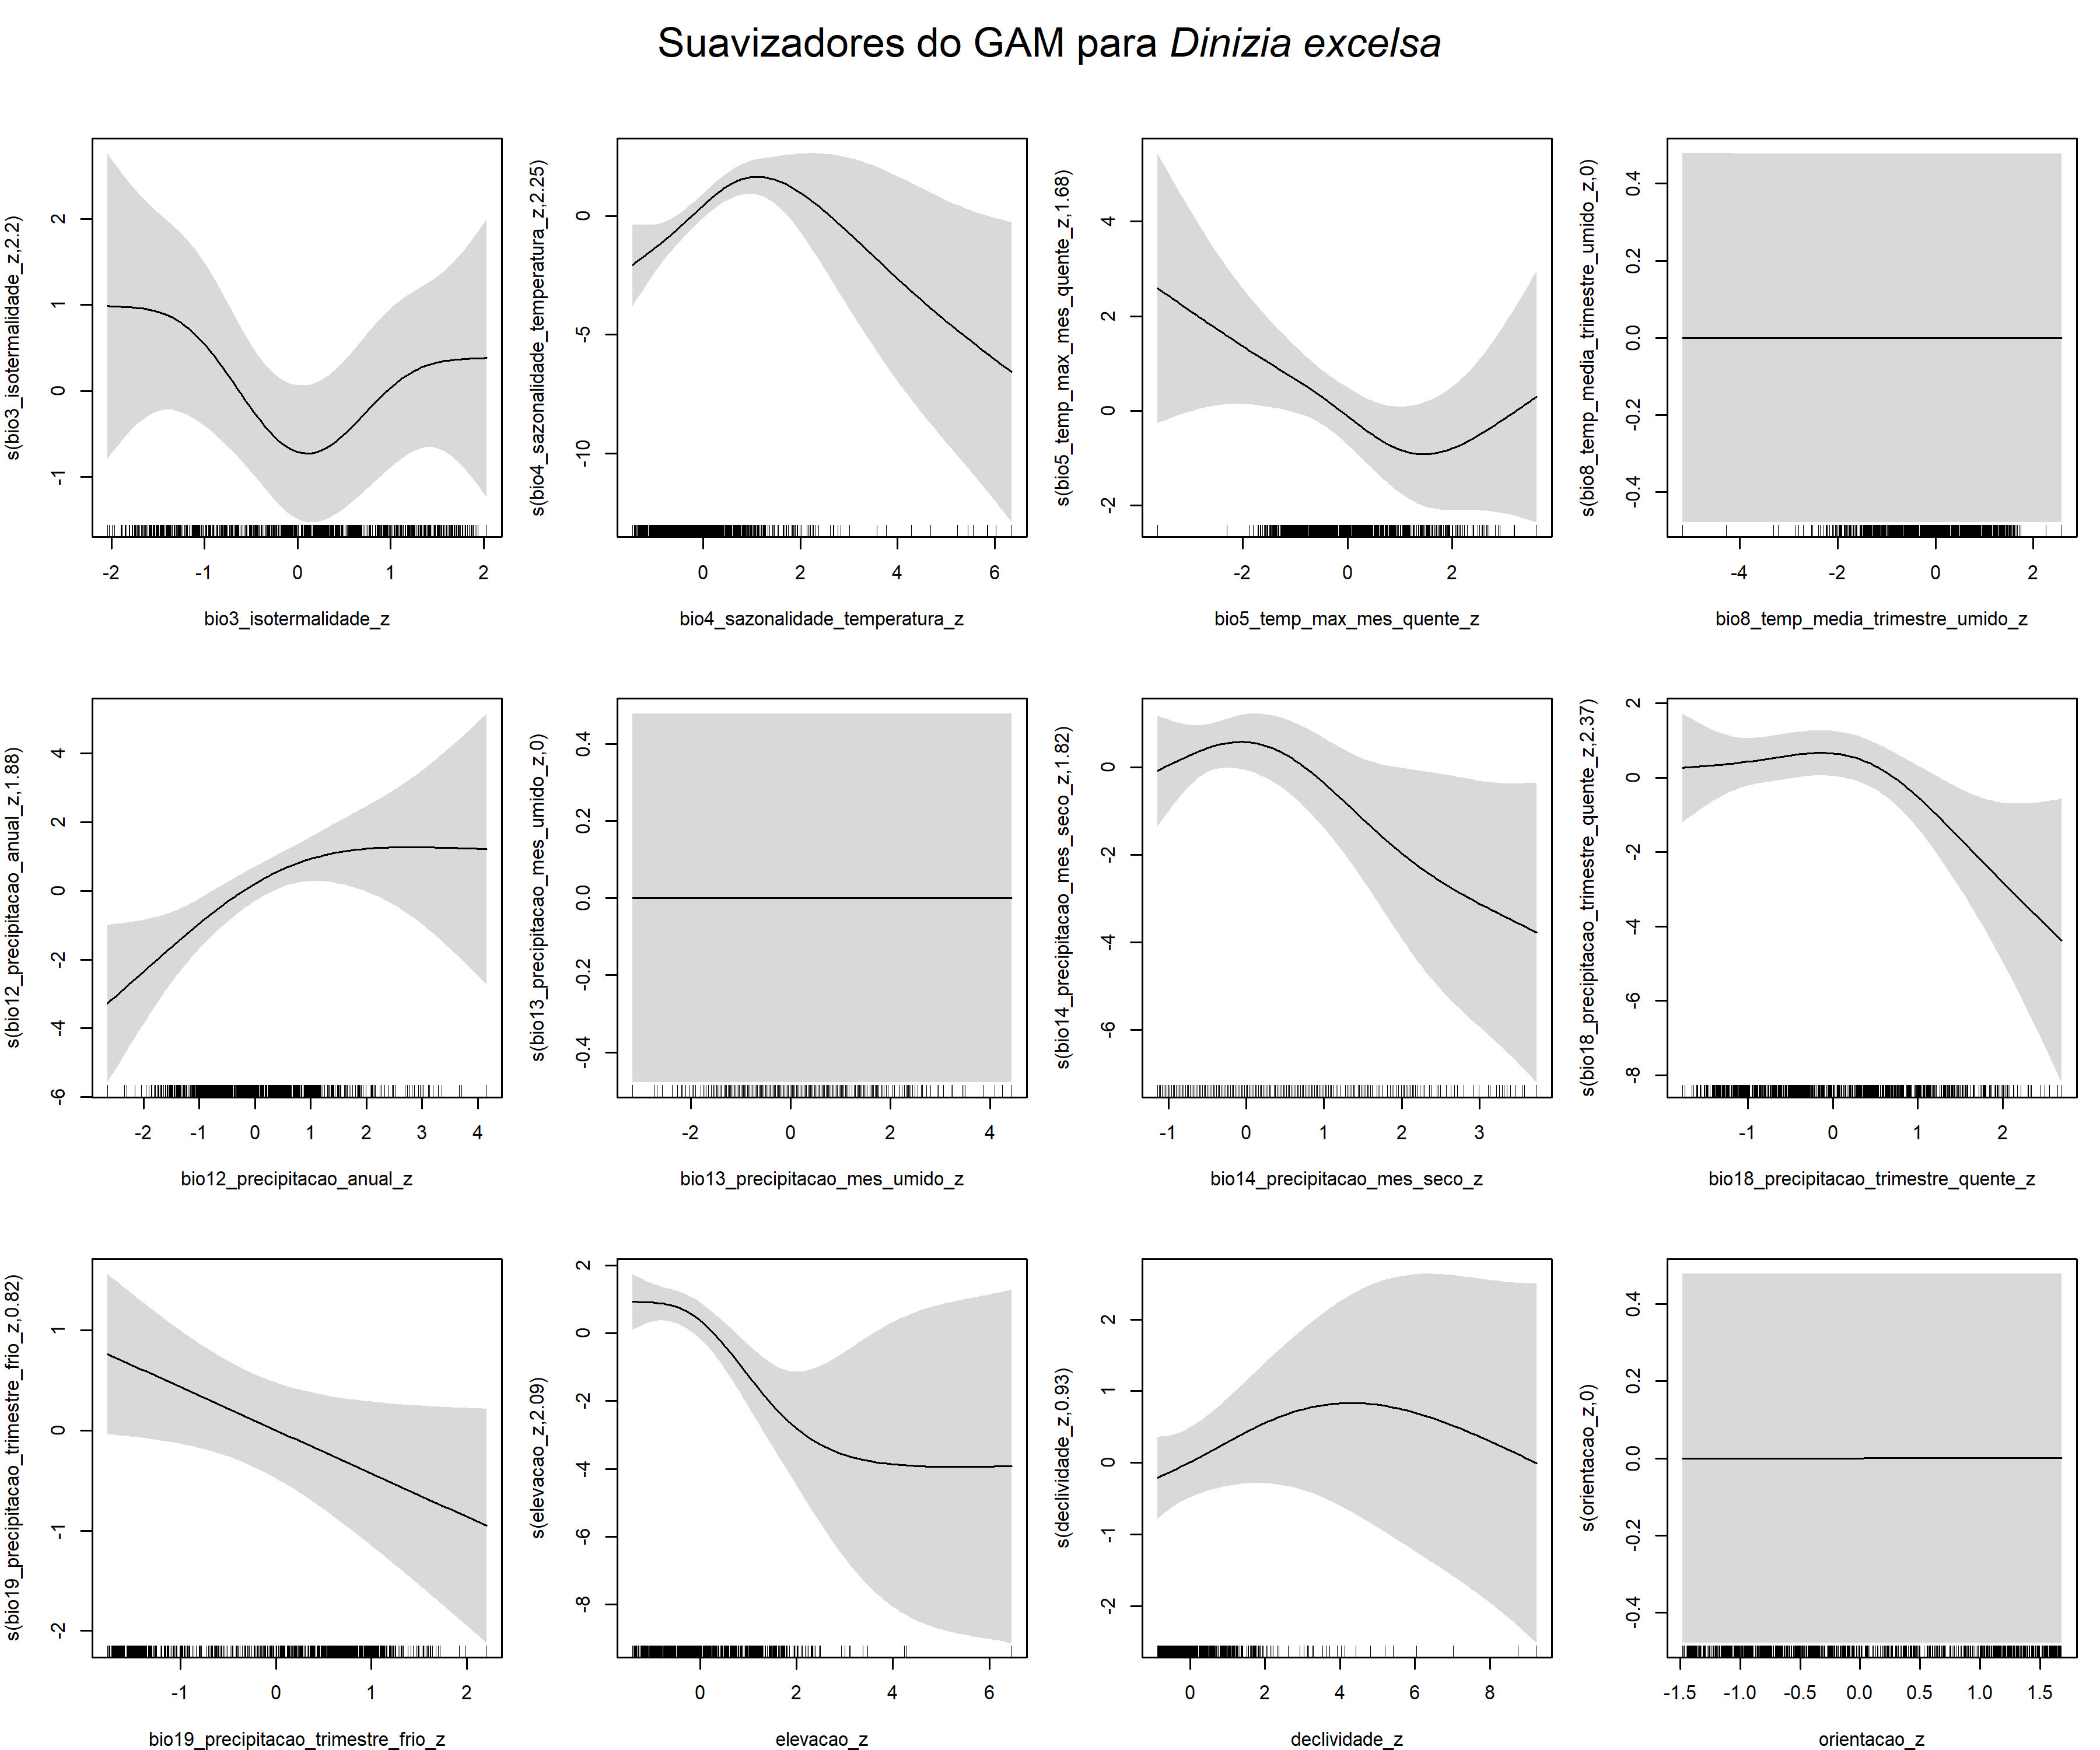
\includegraphics[width=0.96\textwidth]{figuras/unidade07/unidade07_suavizadores_gam.png}
  \caption{Smooth functions estimated by the GAM for the selected environmental predictors. Each panel shows the partial contribution of one variable to environmental suitability for \textit{Dinizia excelsa}.}
  \label{fig:unidade07_suavizadores_gam}
\end{figure}

\section{Model Evaluation}

Predictive performance is evaluated using AUC, TSS, sensitivity, specificity,
and a confusion matrix, enabling comparison with the GLM from Chapter 6.

\rscriptfile{scripts/unidade07/04_avaliar_gam_dinizia.R}

\begin{figure}[H]
  \centering
  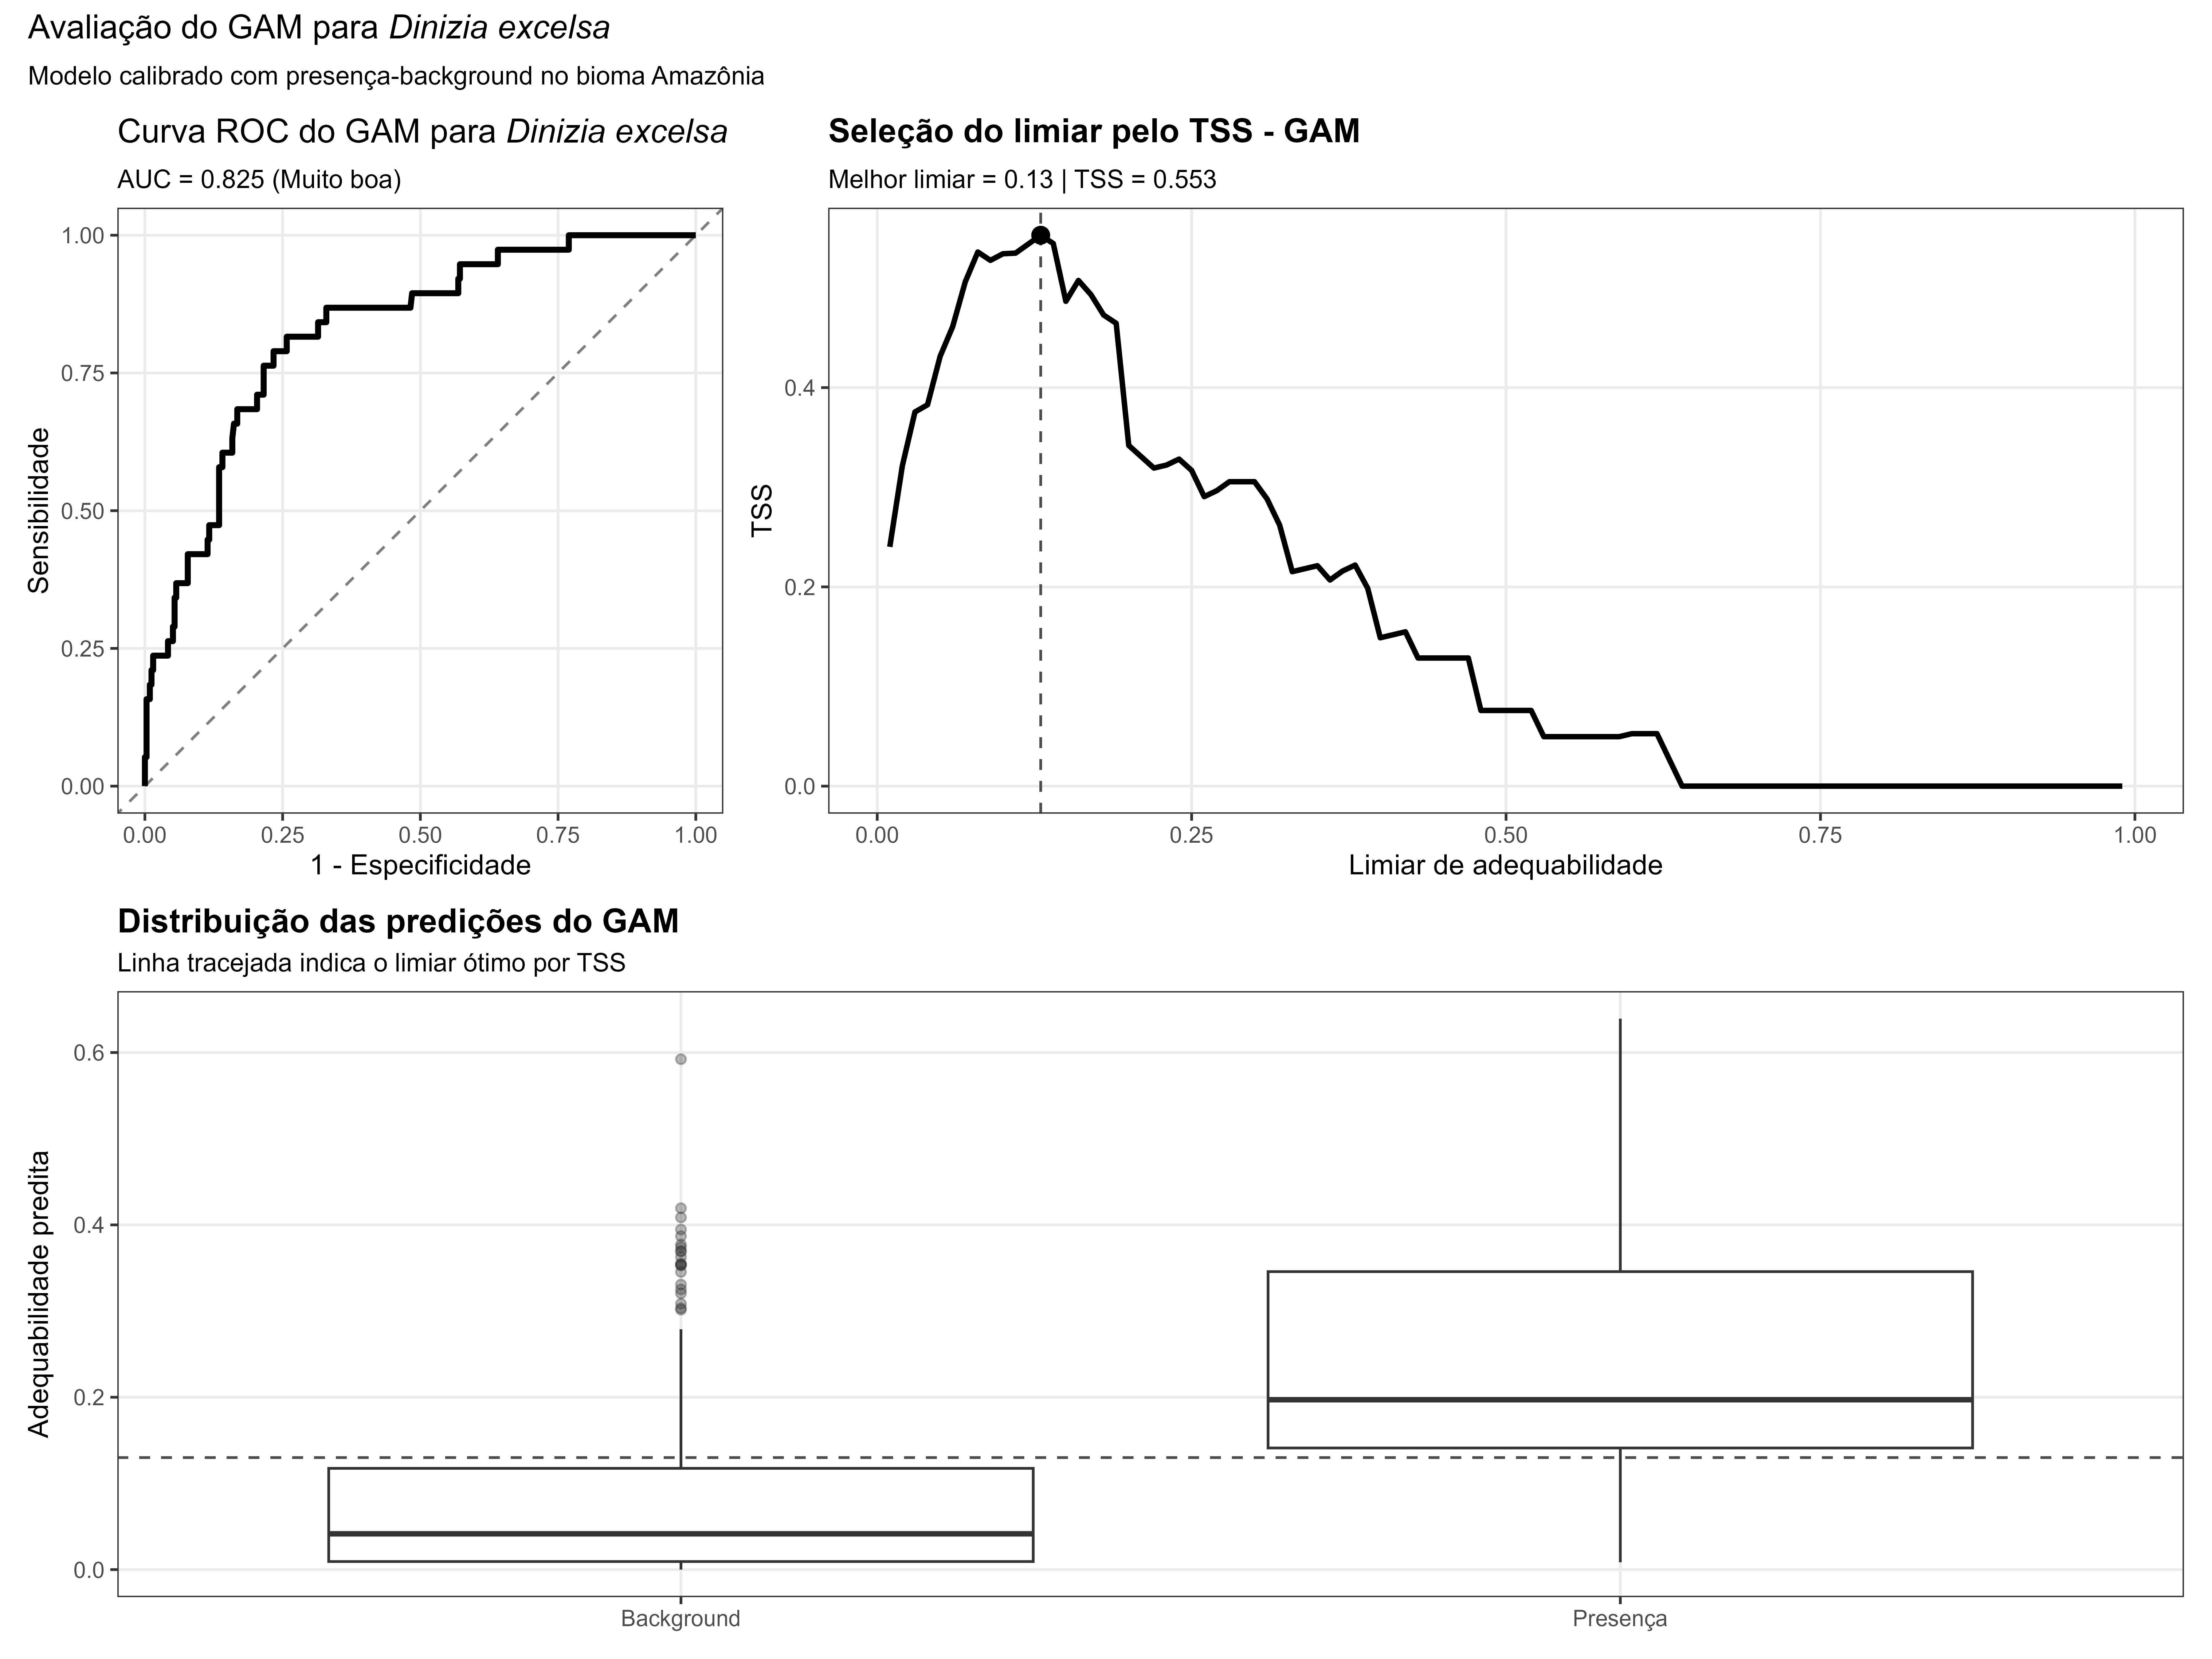
\includegraphics[width=0.78\textwidth]{figuras/unidade07/unidade07_avaliacao_gam_patchwork.png}
  \caption{ROC curve for the GAM fitted to \textit{Dinizia excelsa}.}
  \label{fig:unidade07_roc_gam}
\end{figure}

\section{Current Suitability Map}

The GAM is projected across the accessible area $M$ to produce a continuous map
of current environmental suitability.

\rscriptfile{scripts/unidade07/05_predicao_espacial_gam.R}

\begin{figure}[H]
  \centering
  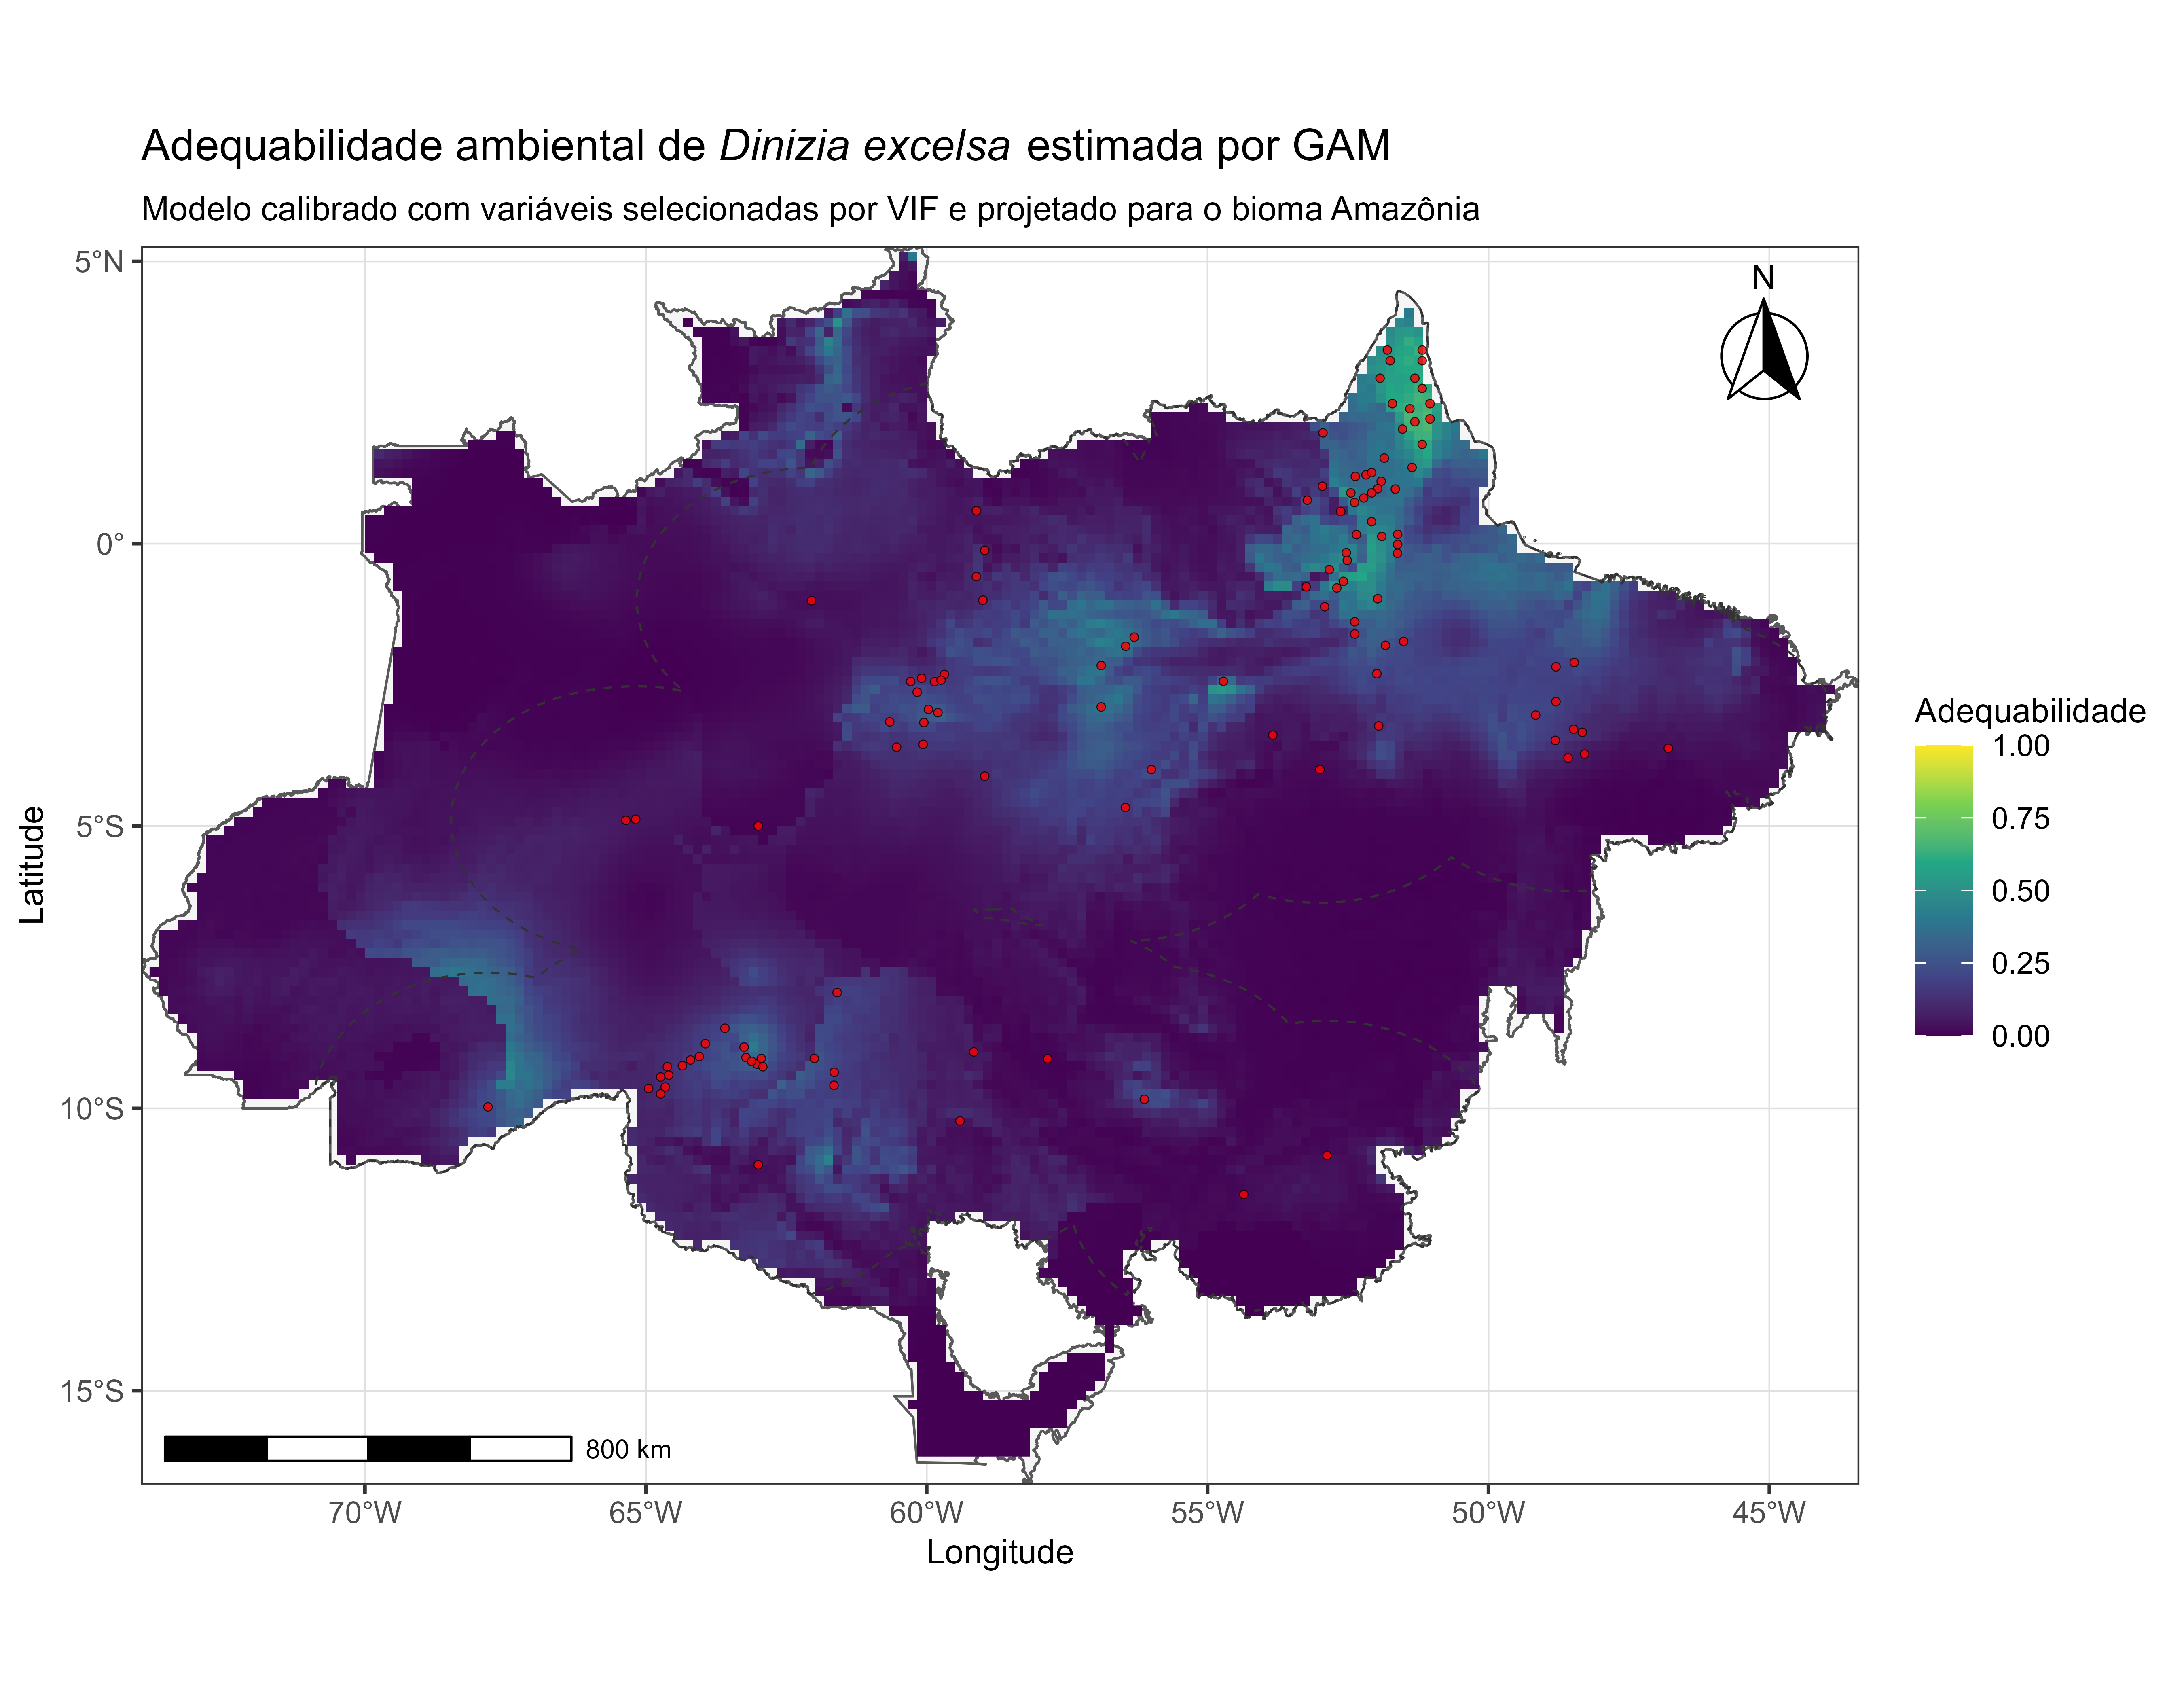
\includegraphics[width=0.88\textwidth]{figuras/unidade07/unidade07_adequabilidade_gam.png}
  \caption{Current environmental suitability for \textit{Dinizia excelsa} estimated by the GAM within the accessible area $M$.}
  \label{fig:unidade07_adequabilidade_gam}
\end{figure}

\section{Partial Response Curves}

GAM partial response curves show flexible responses along environmental
gradients and can reveal suitability ranges, thresholds, and potential climatic
constraints.

\rscriptfile{scripts/unidade07/06_curvas_resposta_gam.R}

\begin{figure}[H]
  \centering
  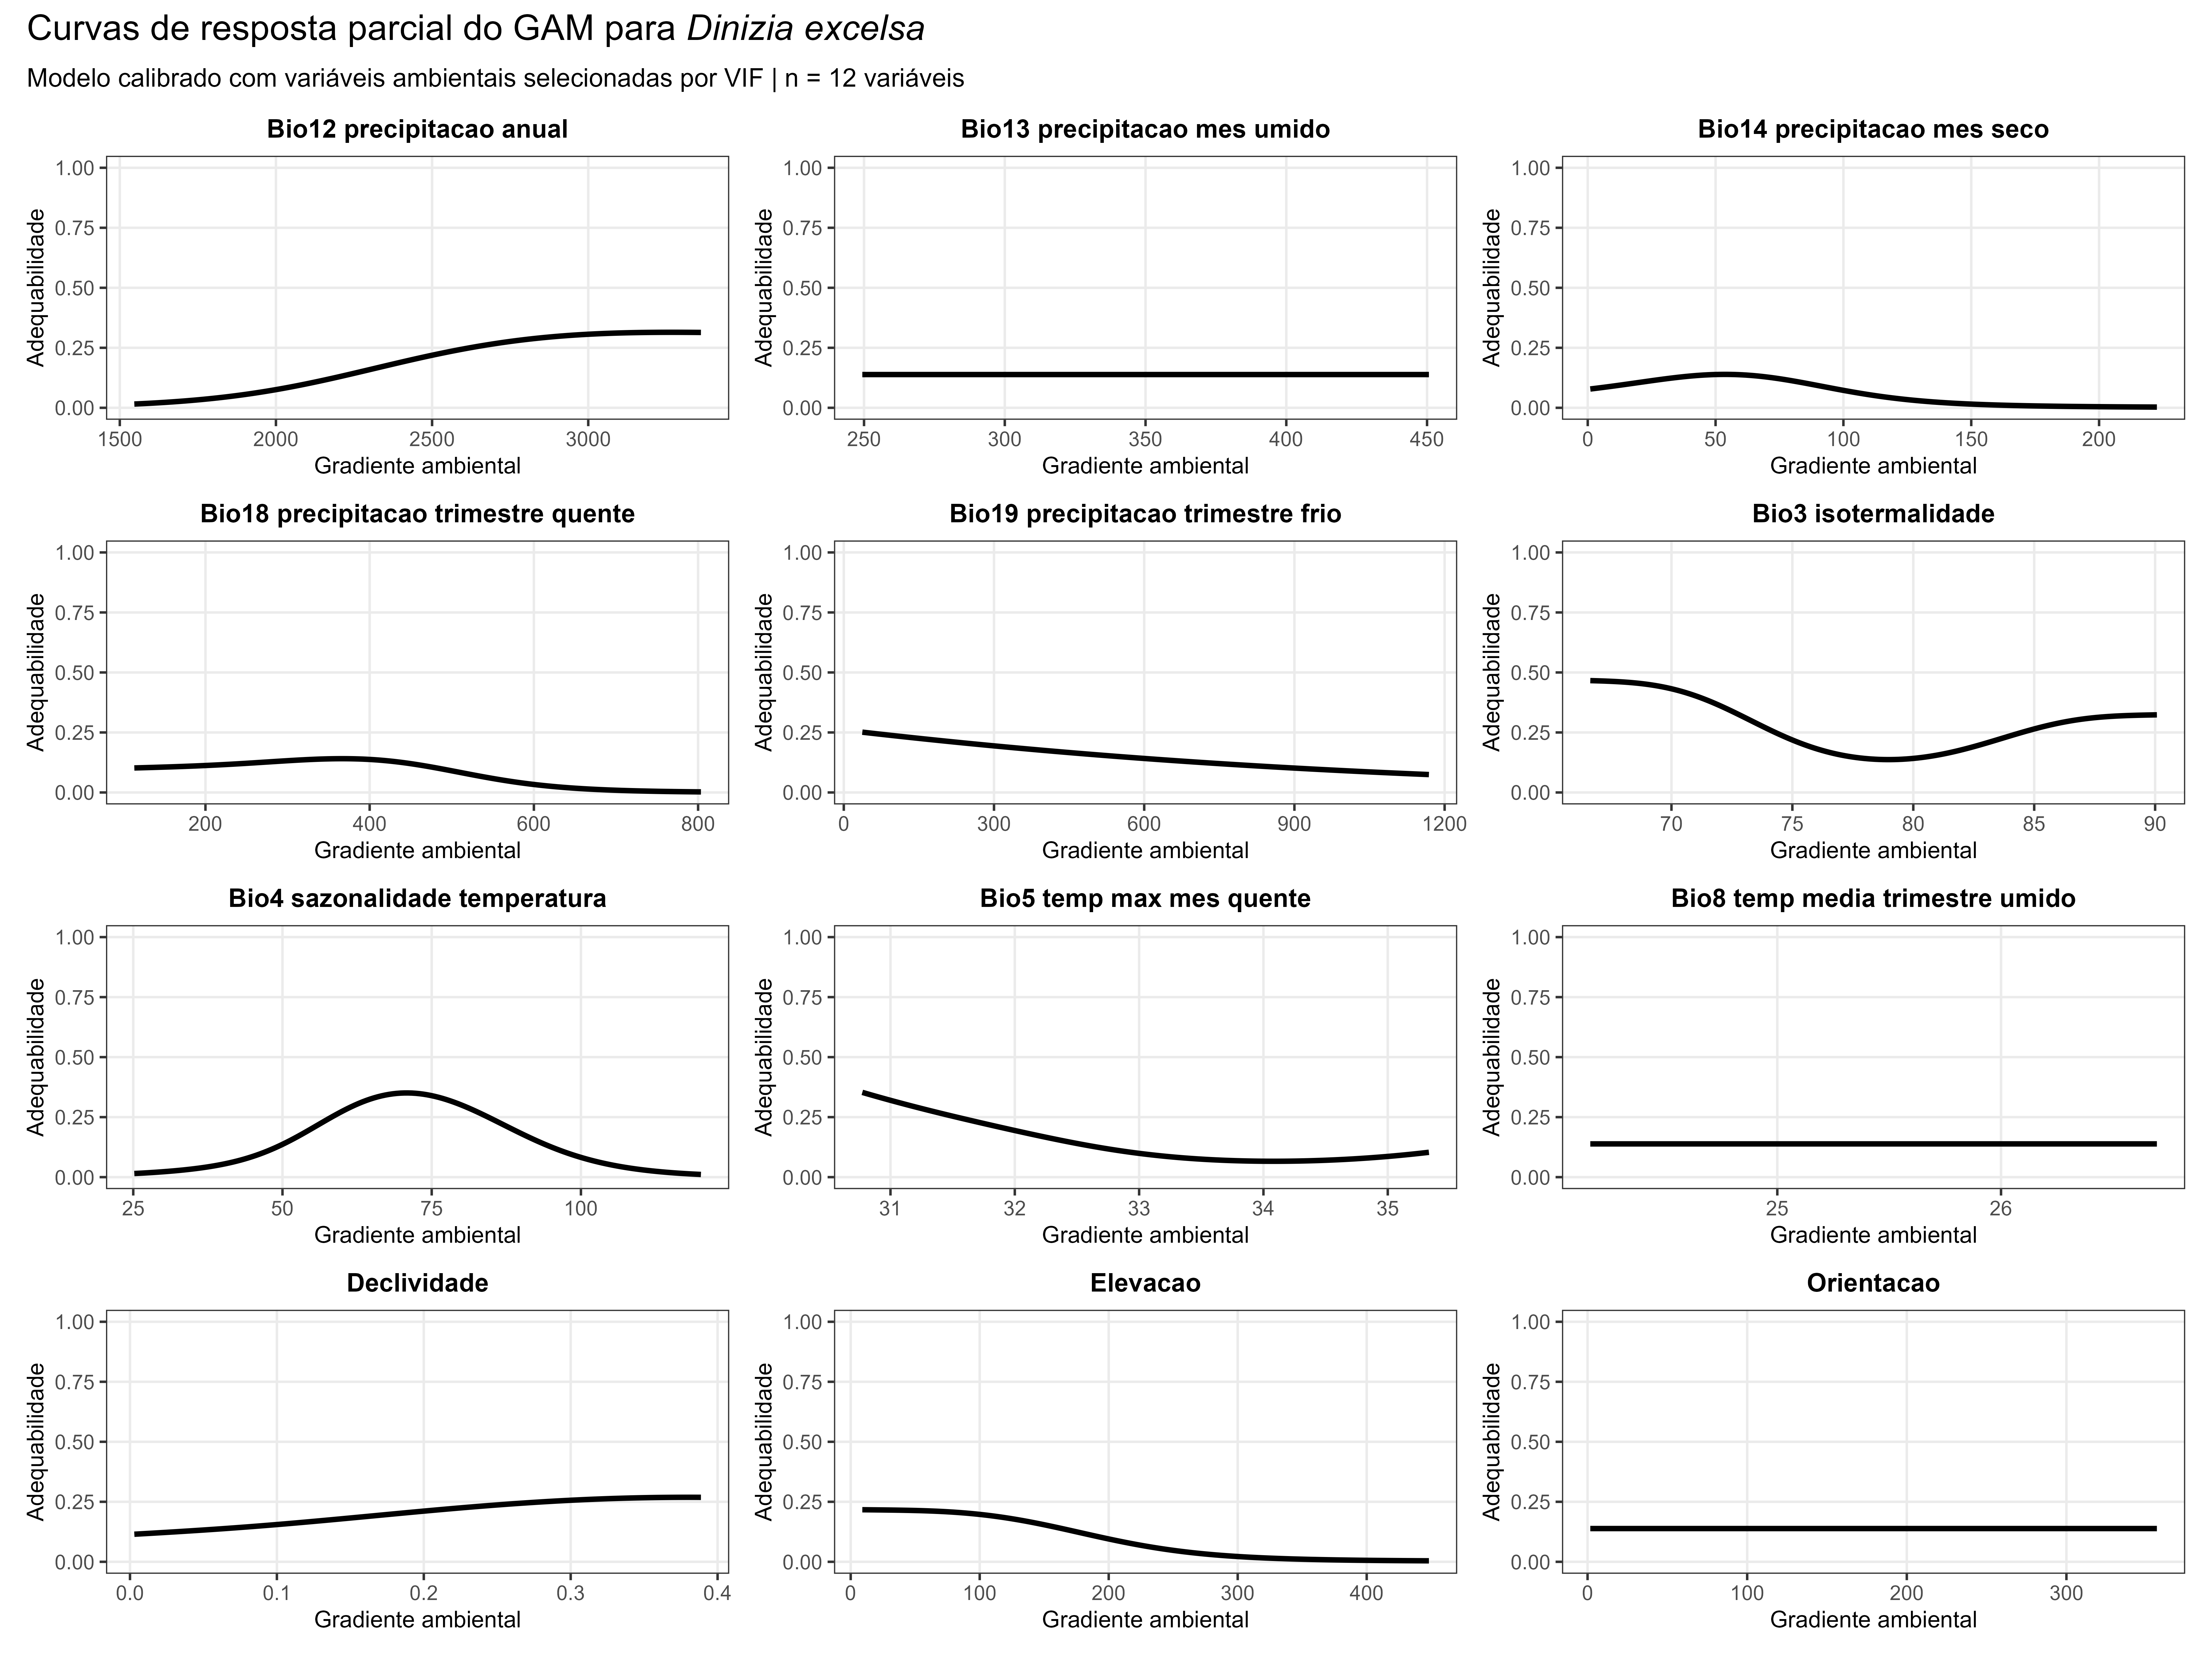
\includegraphics[width=0.96\textwidth]{figuras/unidade07/unidade07_curvas_resposta_gam.png}
  \caption{GAM partial response curves for the selected environmental predictors.}
  \label{fig:unidade07_curvas_resposta_gam}
\end{figure}

\section{Comparing GLM and GAM}

Comparison of the GLM and GAM reveals how greater flexibility changes the
projected spatial distribution and environmental response curves.

\rscriptfile{scripts/unidade07/07_comparar_glm_gam.R}

\begin{figure}[H]
  \centering
  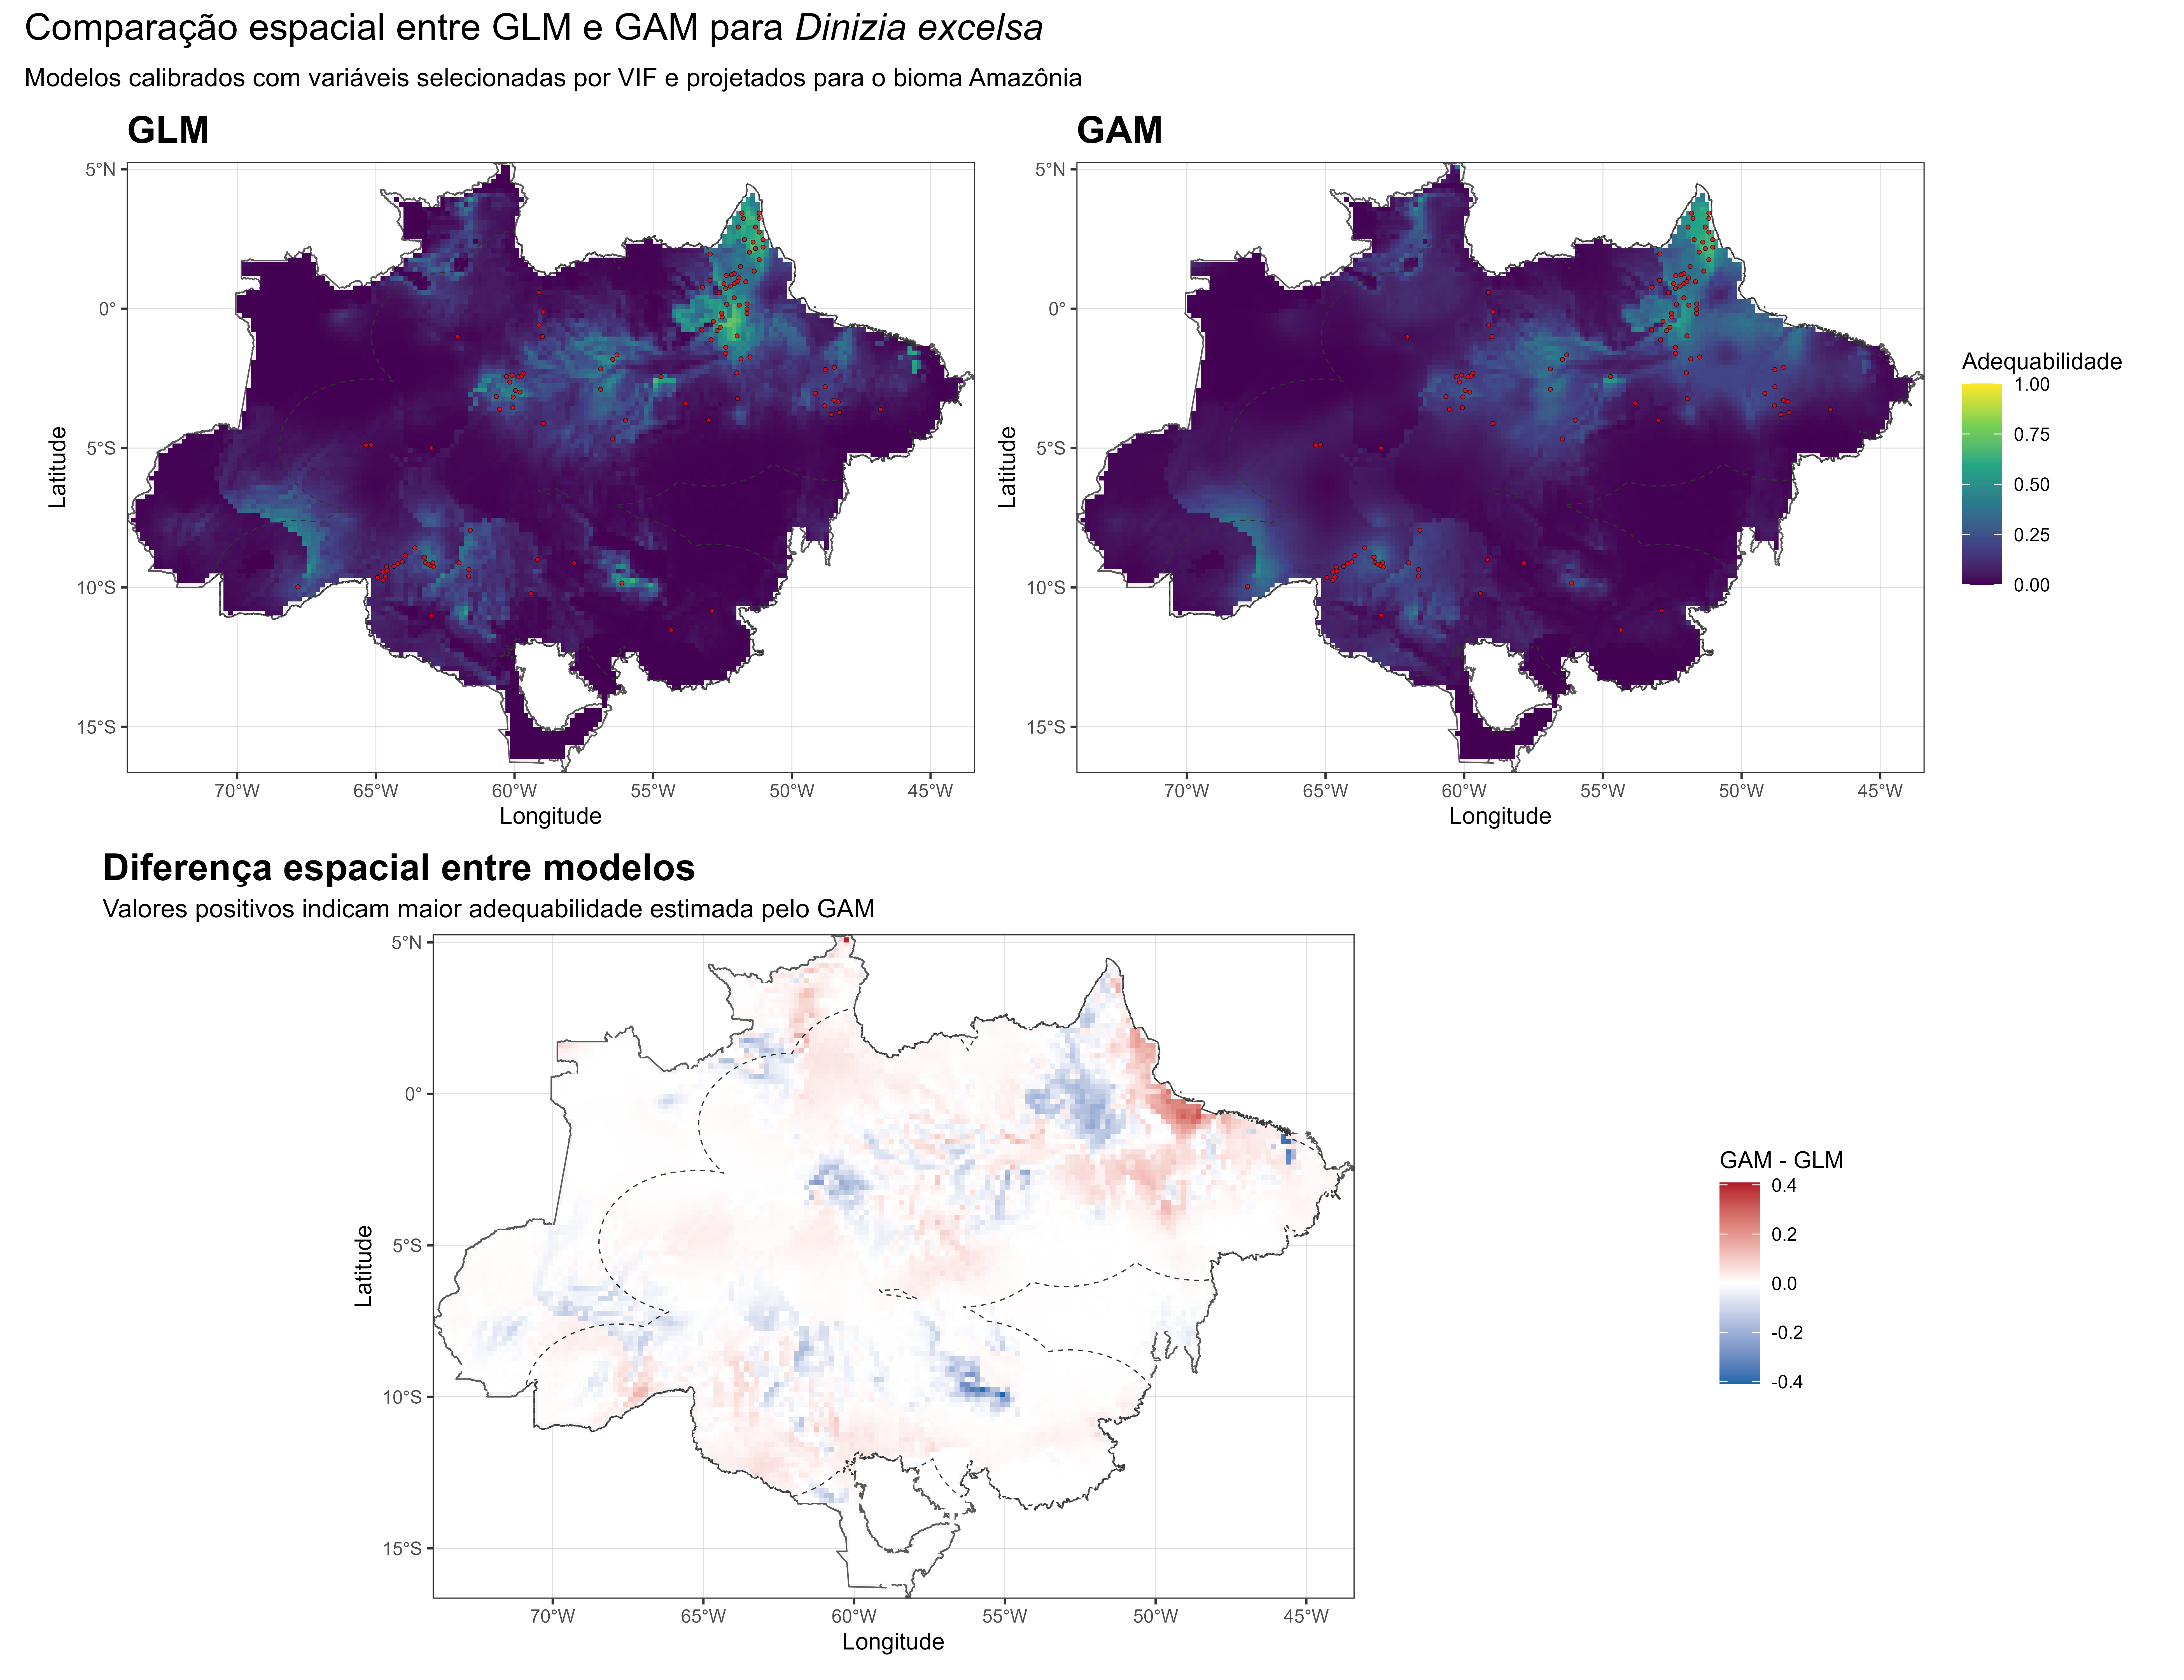
\includegraphics[width=0.96\textwidth]{figuras/unidade07/unidade07_comparacao_glm_gam.png}
  \caption{Comparison of suitability maps estimated by GLM and GAM for \textit{Dinizia excelsa}.}
  \label{fig:unidade07_comparacao_glm_gam}
\end{figure}

\section{Complete Pipeline}
\rscriptfile{scripts/unidade07/08_pipeline_gam.R}

\section{Chapter Summary}

The GAM occupies an intermediate position between simple parametric models and
machine-learning algorithms. It remains interpretable while representing
nonlinear environmental relationships. For \textit{Dinizia excelsa}, it makes
flexible ecological responses to the selected gradients visible.

\begin{conceito}[title={\faBook\quad Key message}]
GAMs are particularly useful when species are expected to respond nonlinearly
to environmental gradients. They offer a balance among flexibility, ecological
interpretation, and predictive performance.
\end{conceito}

\section{Review Exercises}
\begin{enumerate}
  \item Explain the difference between a GLM and a GAM.
  \item What does a smooth function represent?
  \item Why must $k$ be selected carefully?
  \item Why can GAMs capture nonlinear ecological responses?
  \item What is overfitting in SDM?
  \item How do partial response curves support ecological interpretation?
  \item Compare the advantages and limitations of GLMs and GAMs in SDM.
\end{enumerate}

\chapter[Random Forest]{Applied Random Forest}

\begin{objetivos}
By the end of this chapter, readers should understand the Random Forest
algorithm; fit presence--background models for \textit{Dinizia excelsa};
control complexity to reduce overfitting; evaluate performance with independent
test data; compare out-of-bag (OOB) and test performance; interpret variable
importance and partial response curves; produce suitability maps; and recognize
limitations of machine-learning algorithms in SDM.
\end{objetivos}

\section{Introduction}

Random Forest is a machine-learning algorithm based on many decision trees.
Each tree is fitted to a sample of observations and a random subset of
predictors. Final predictions are obtained by averaging across trees for
regression or probability estimation, or by majority vote for classification
\parencite{breiman2001random,cutler2007random,guisan2017habitat}.

Random Forest is frequently used in SDM because it represents nonlinear
relationships, predictor interactions, and complex environmental responses.
This flexibility requires caution: a model can appear excellent on calibration
data yet generalize poorly across space or time.

\begin{conceito}[title={\faBook\quad Random Forest in SDM}]
Random Forest combines many decision trees to estimate complex relationships
between occurrence and environment. Its strength is flexibility; its risk is
overfitting when validation is not adequately controlled.
\end{conceito}

\section{Overfitting in Random Forest}

Very high metrics, such as an AUC close to 1, may indicate excellent
discrimination but can also signal overfitting, especially in the presence of
spatial autocorrelation, excessive background samples, redundant predictors, or
nonindependent validation.

Four strategies are used to reduce this risk:
\begin{itemize}
  \item a stratified training--test split;
  \item predictors retained after correlation and VIF analysis;
  \item complexity control through \texttt{mtry}, \texttt{min.node.size}, and \texttt{sample.fraction}; and
  \item comparison of OOB and test-set performance.
\end{itemize}

\begin{atencao}[title={\faExclamationTriangle\quad An extremely high AUC requires caution}]
An AUC near 1 does not necessarily identify an ecologically excellent model. It
may reflect overfitting, spatial bias, an easily distinguished background, or
nonindependent validation.
\end{atencao}

\section{Data Preparation}

The analysis uses the Chapter 5 dataset: real \textit{Dinizia excelsa}
presences, background sampled within $M$, and predictors retained in Chapter 4.

\rscriptfile{scripts/unidade08/01_estrutura_pastas.R}
\rscriptfile{scripts/unidade08/02_preparar_dados_rf.R}

\section{Controlled Random Forest Fitting}

The model is fitted with \texttt{ranger}, using its probability-forest output.
Because the contrast class is background rather than confirmed absence, this
numeric output is interpreted as a relative score, not absolute occurrence
probability.
Moderate \texttt{mtry}, a larger-than-default \texttt{min.node.size}, and a
\texttt{sample.fraction} below 1 constrain complexity.

\rscriptfile{scripts/unidade08/03_ajustar_rf_dinizia.R}

\begin{figure}[H]
  \centering
  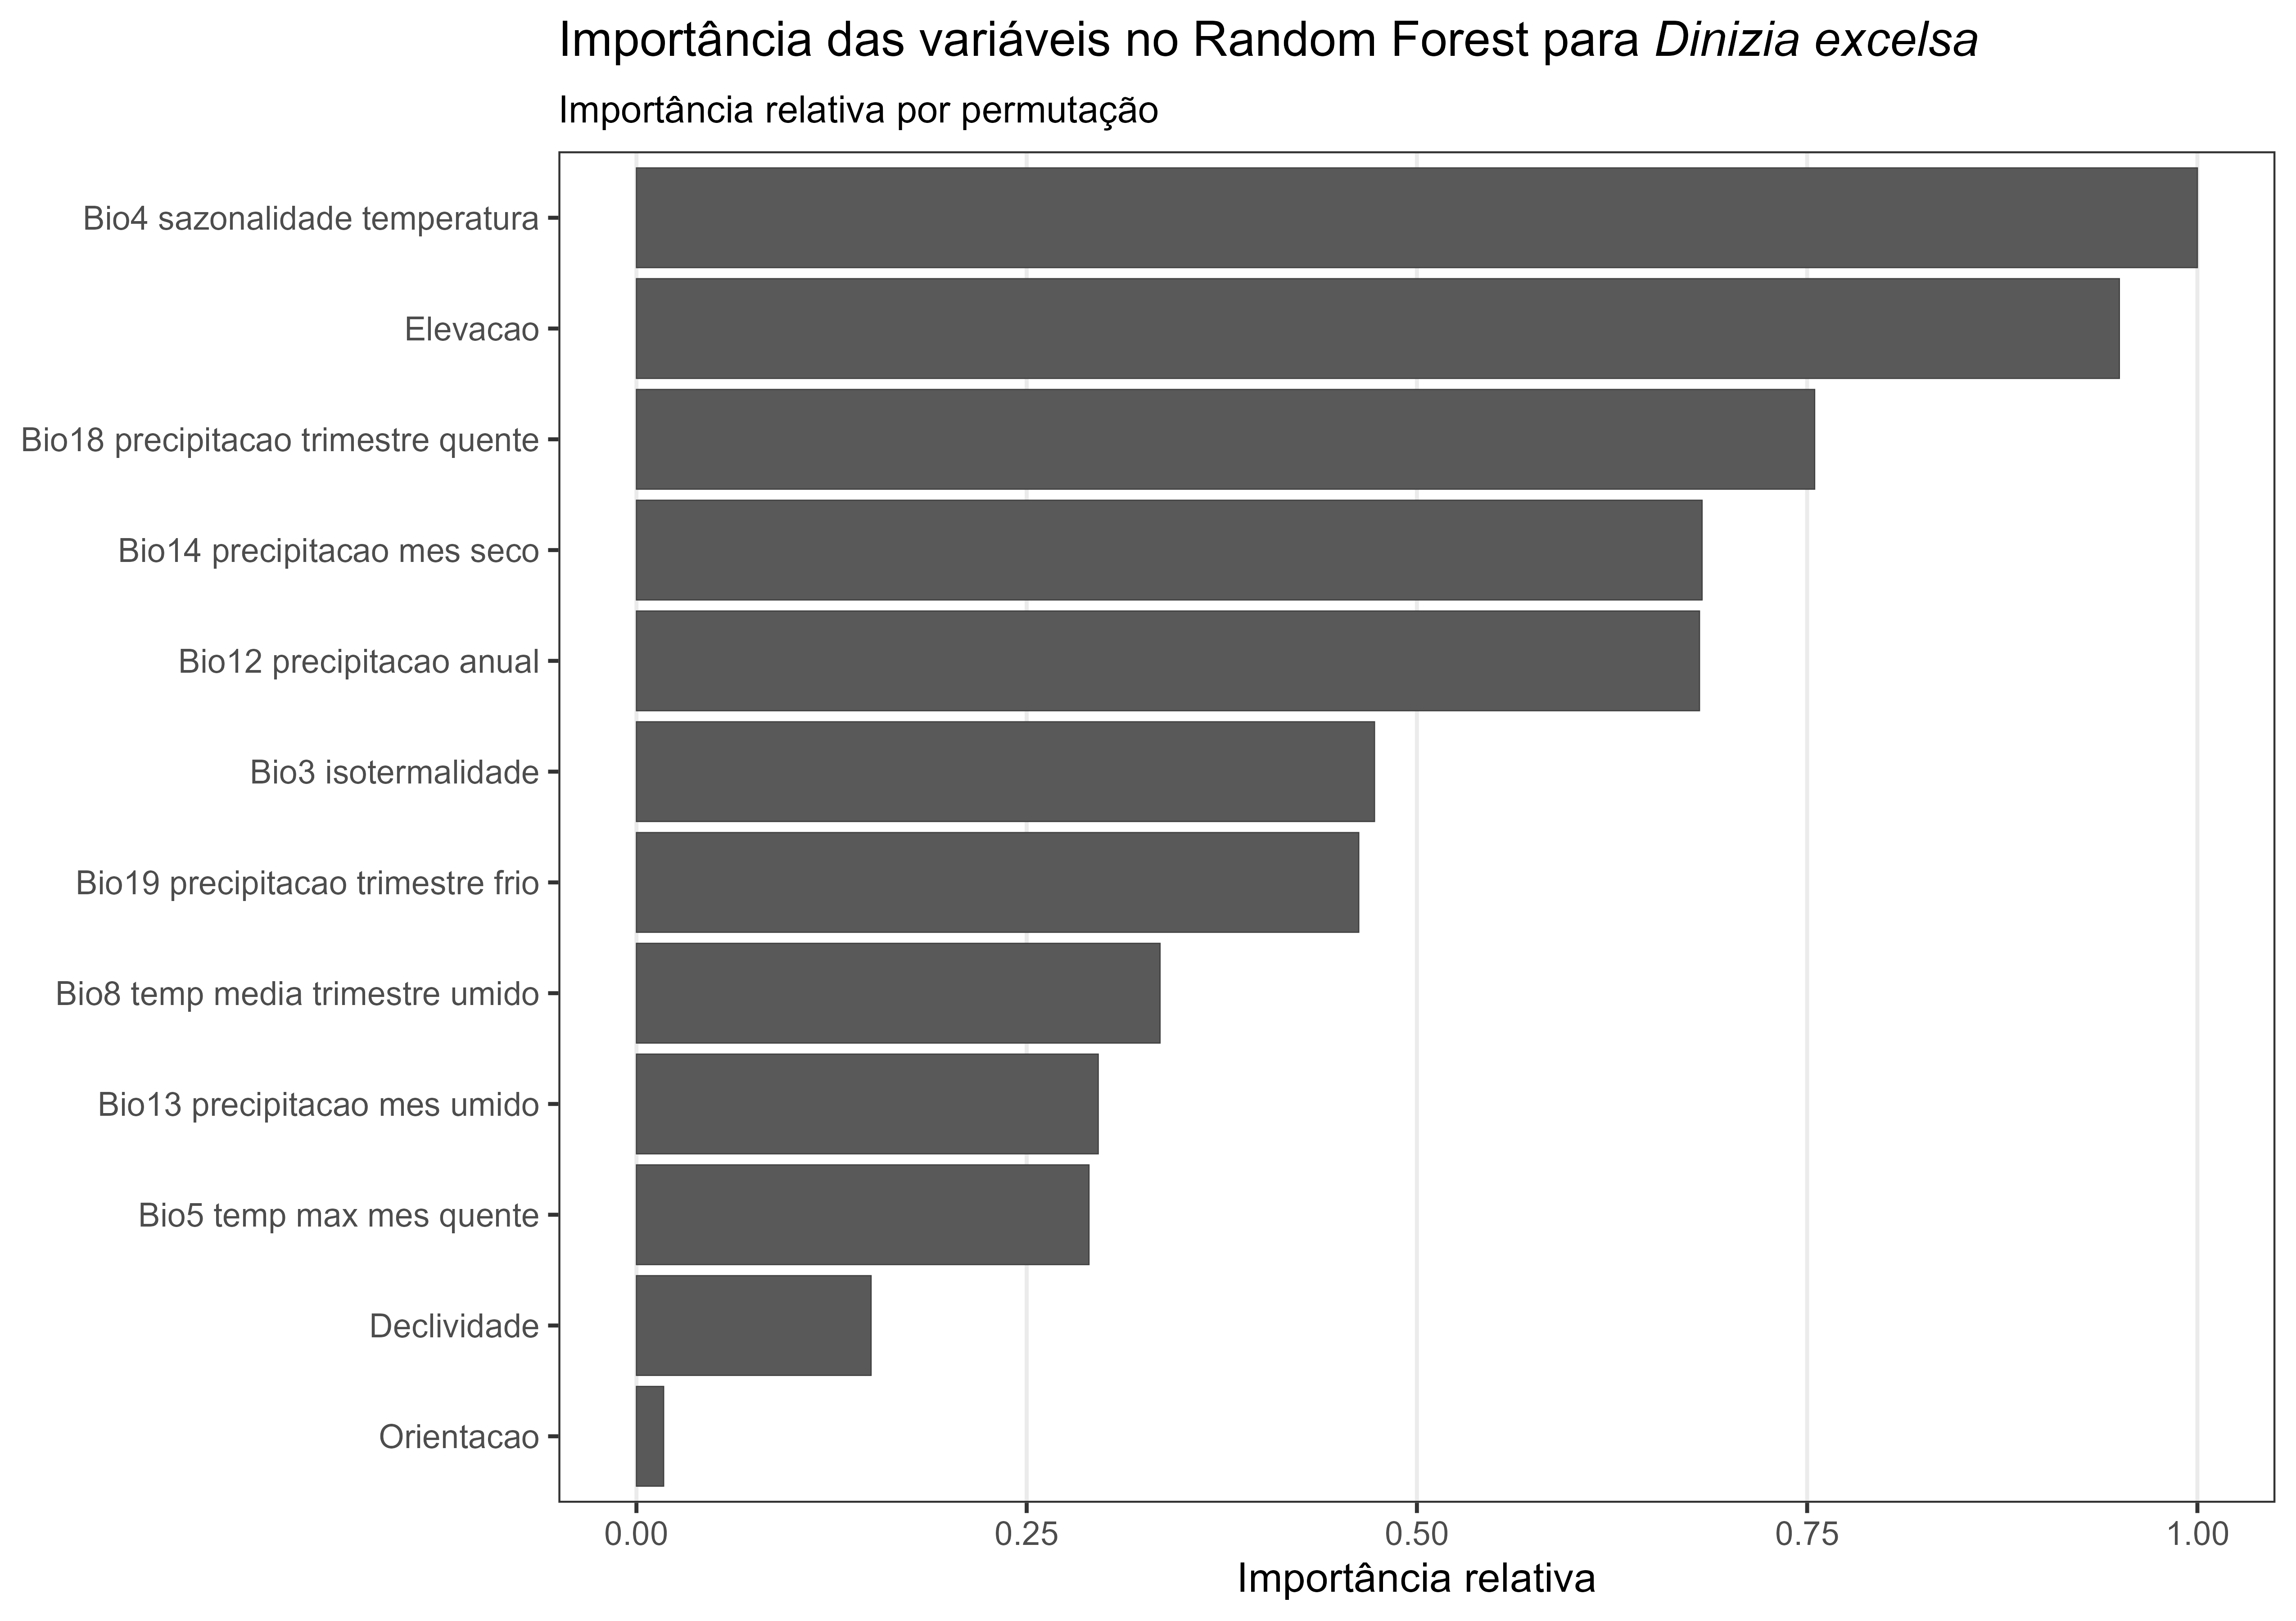
\includegraphics[width=0.86\textwidth]{figuras/unidade08/unidade08_importancia_variaveis_rf.png}
  \caption{Environmental-predictor importance in the Random Forest fitted to \textit{Dinizia excelsa}.}
  \label{fig:unidade08_importancia_rf}
\end{figure}

\section{Model Evaluation}

Performance is evaluated on the test set rather than the training data. OOB AUC
and test AUC are also compared; large differences may indicate instability or
overfitting.

\rscriptfile{scripts/unidade08/04_avaliar_rf_dinizia.R}

\begin{figure}[H]
  \centering
  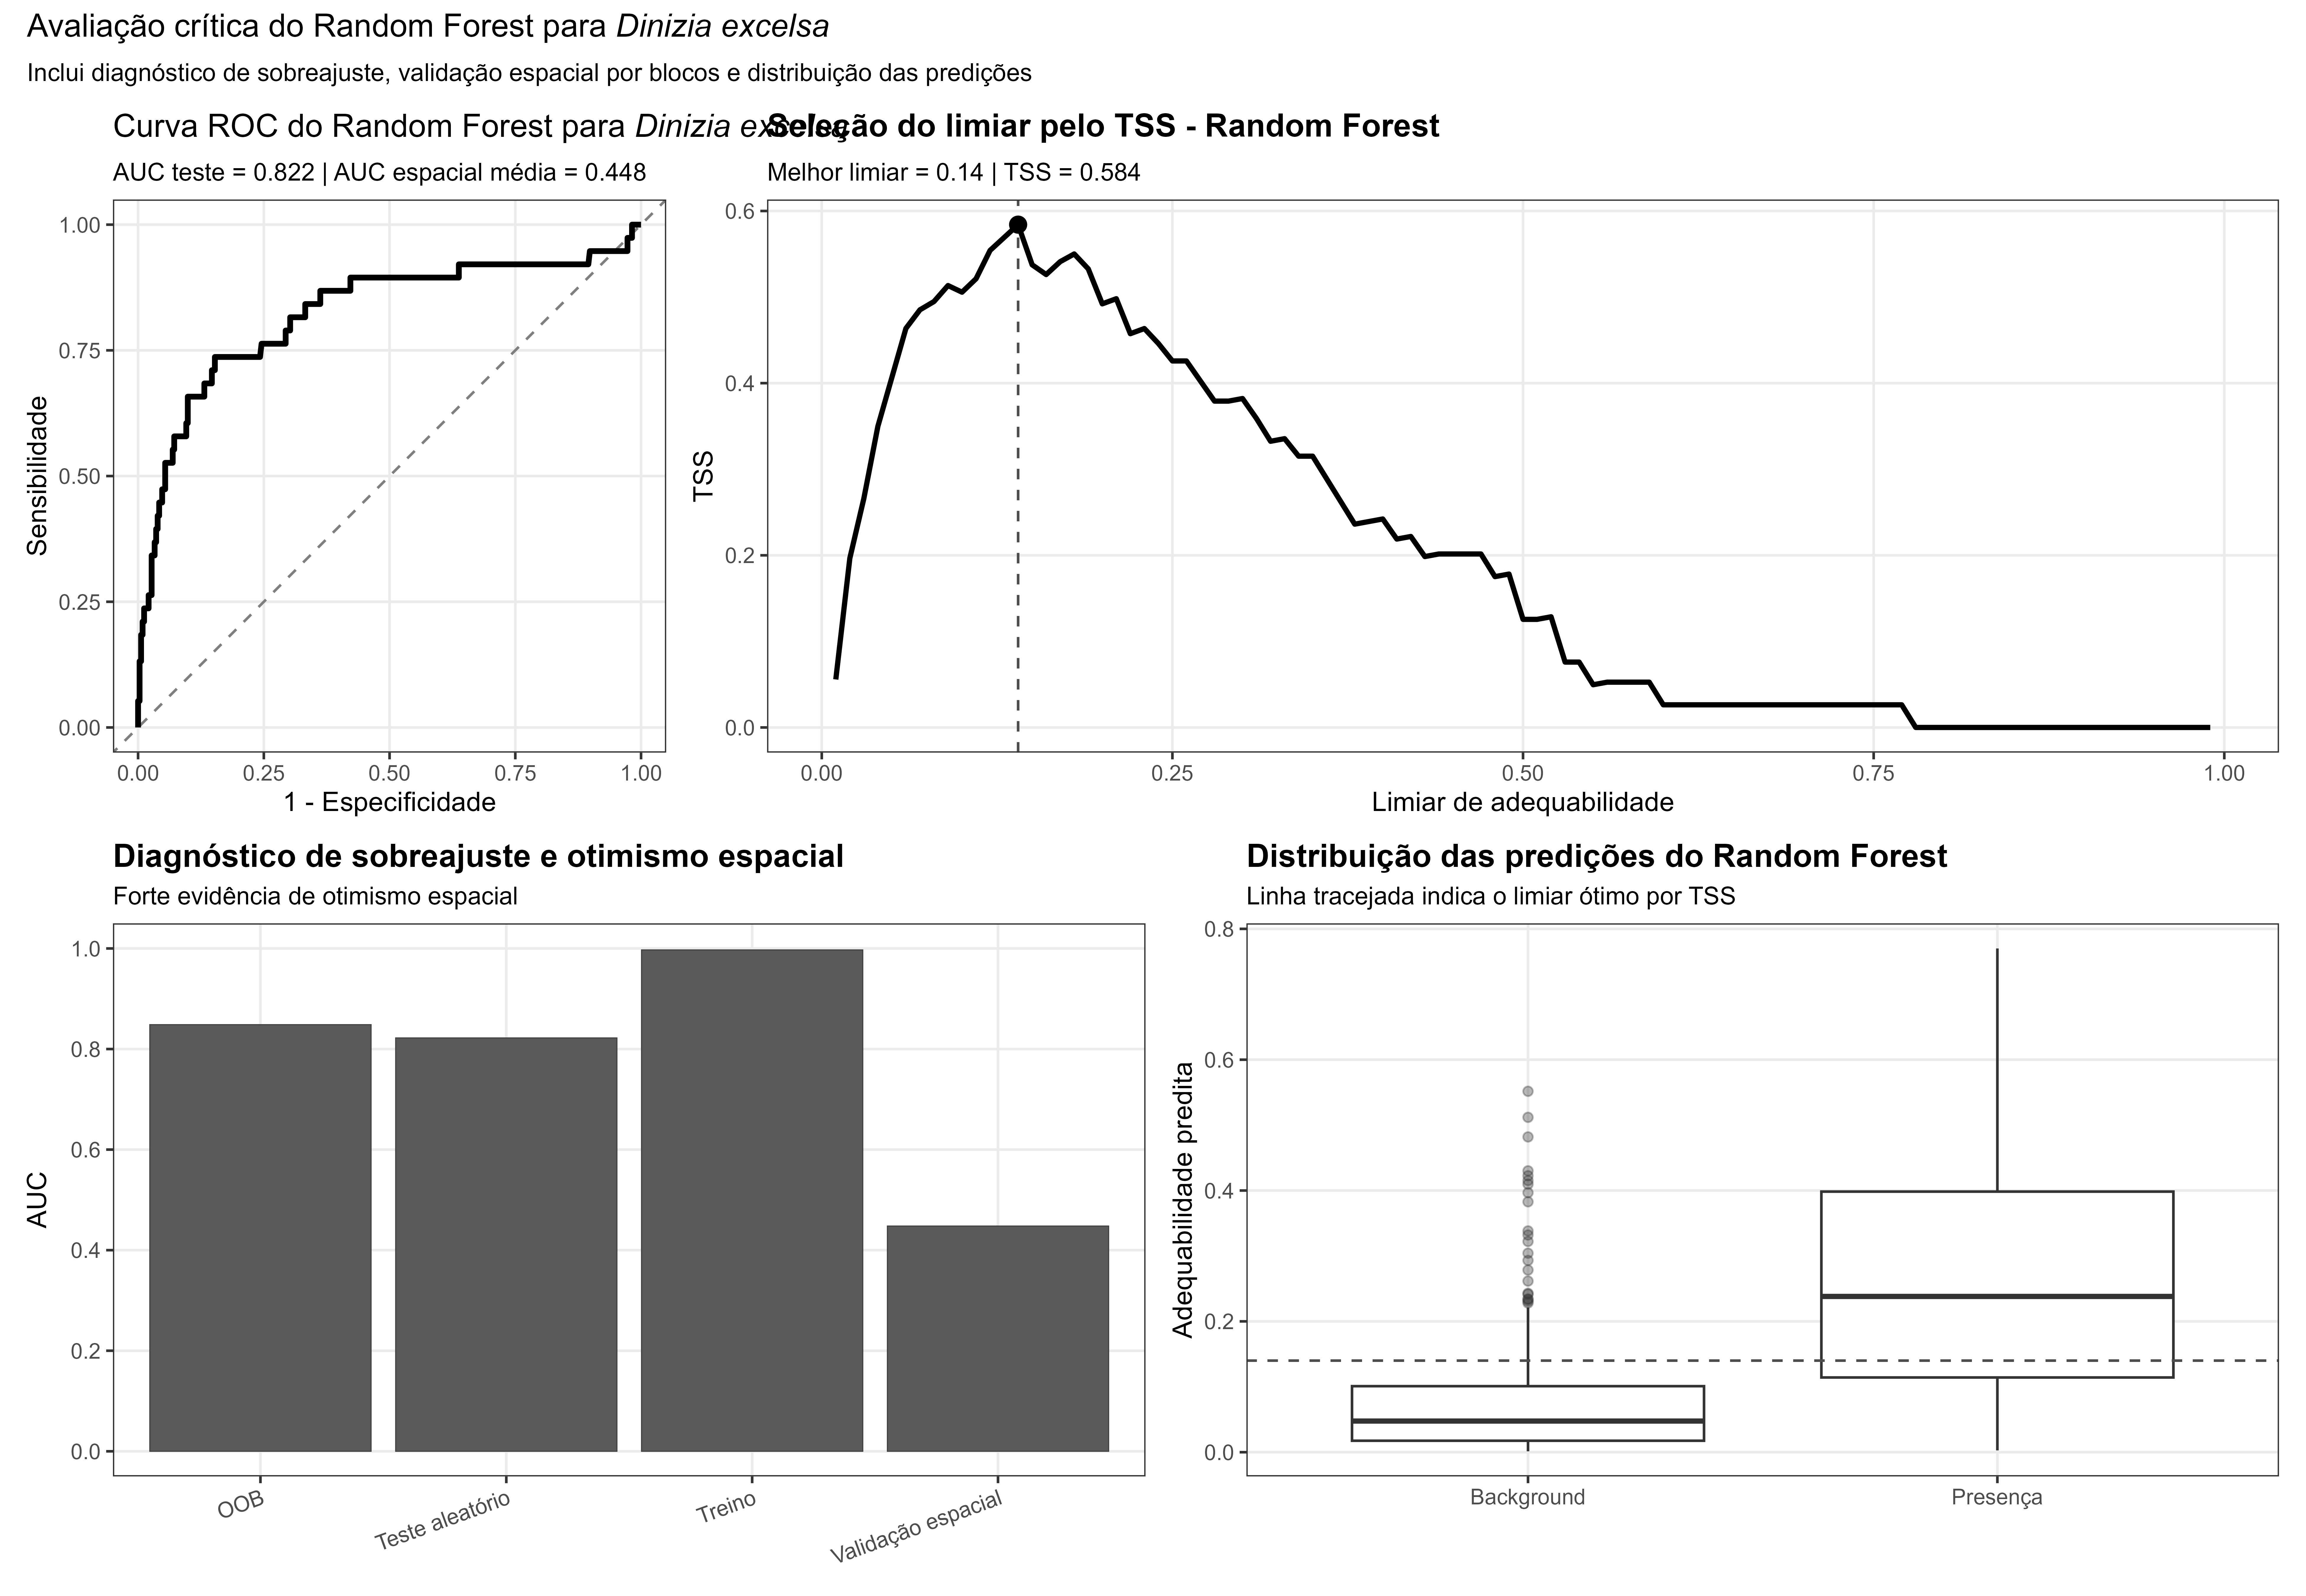
\includegraphics[width=0.78\textwidth]{figuras/unidade08/unidade08_avaliacao_rf_patchwork.png}
  \caption{ROC curve for the Random Forest evaluated on the test set.}
  \label{fig:unidade08_roc_rf}
\end{figure}

\section{Current Suitability Map}

After evaluation, the model is projected across $M$ to produce a continuous
map of current environmental suitability.

\rscriptfile{scripts/unidade08/05_predicao_espacial_rf.R}

\begin{figure}[H]
  \centering
  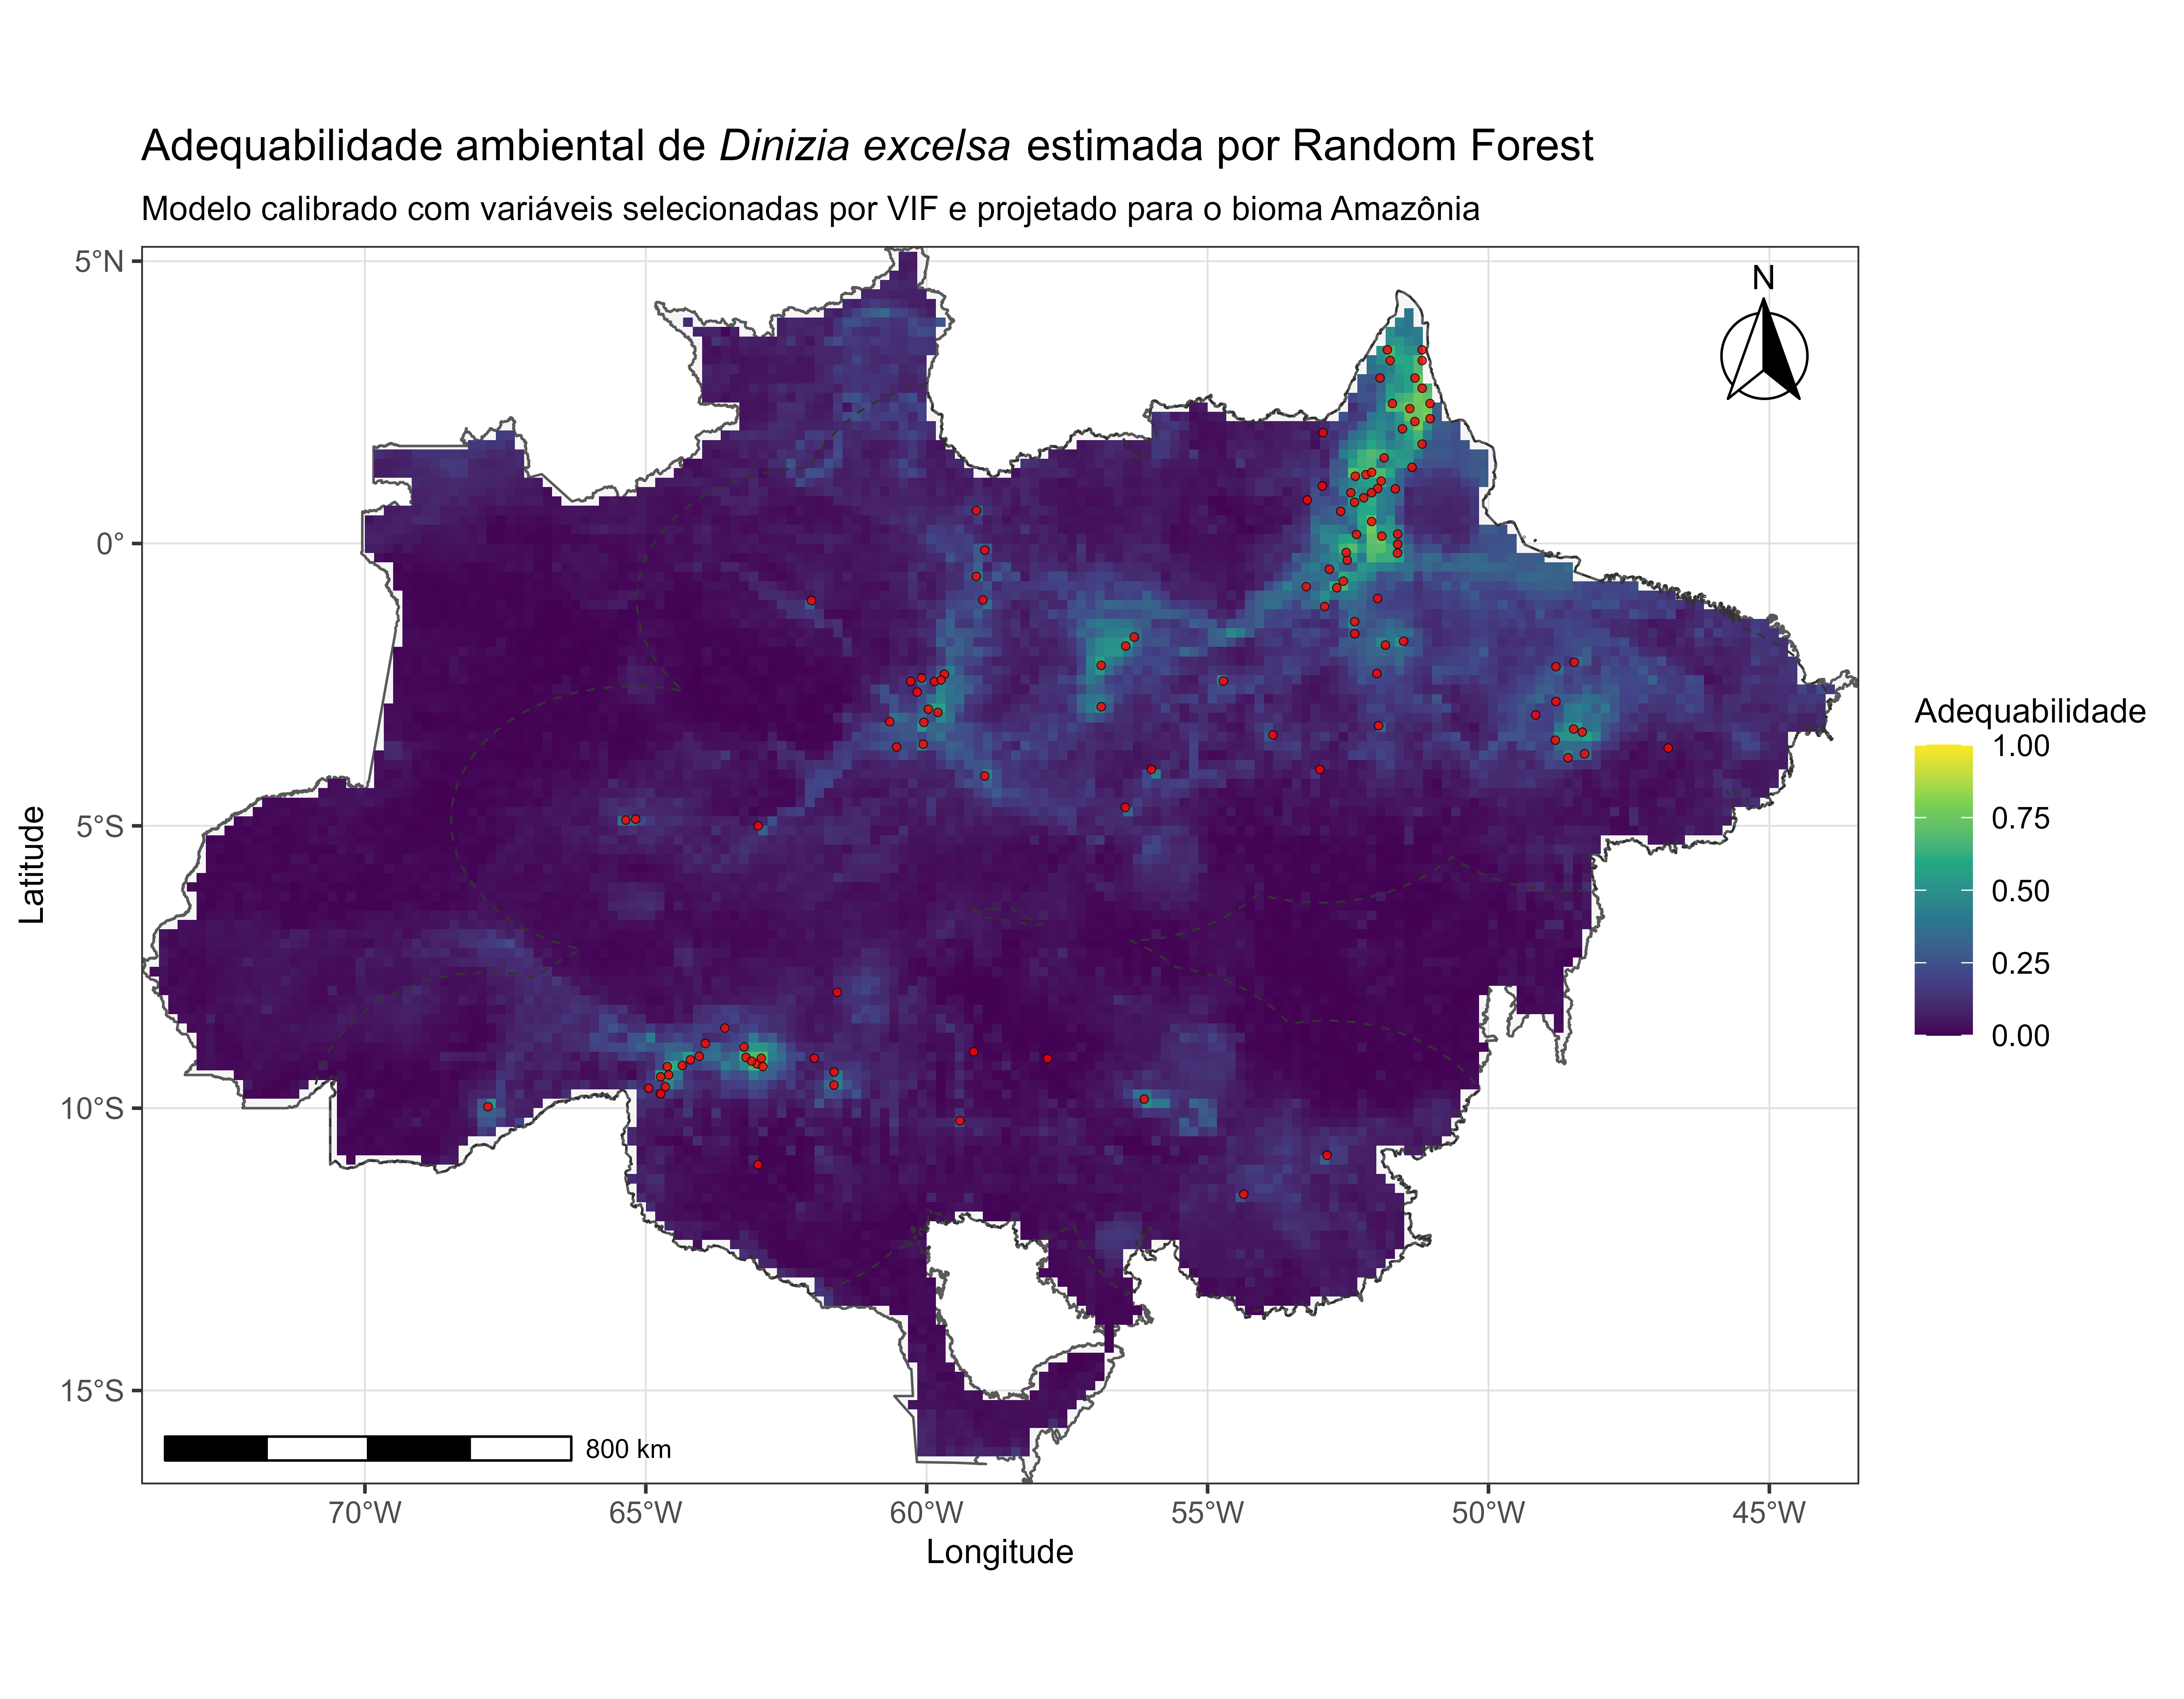
\includegraphics[width=0.88\textwidth]{figuras/unidade08/unidade08_adequabilidade_rf.png}
  \caption{Current environmental suitability for \textit{Dinizia excelsa} estimated by Random Forest within $M$.}
  \label{fig:unidade08_adequabilidade_rf}
\end{figure}

\begin{figure}[H]
  \centering
  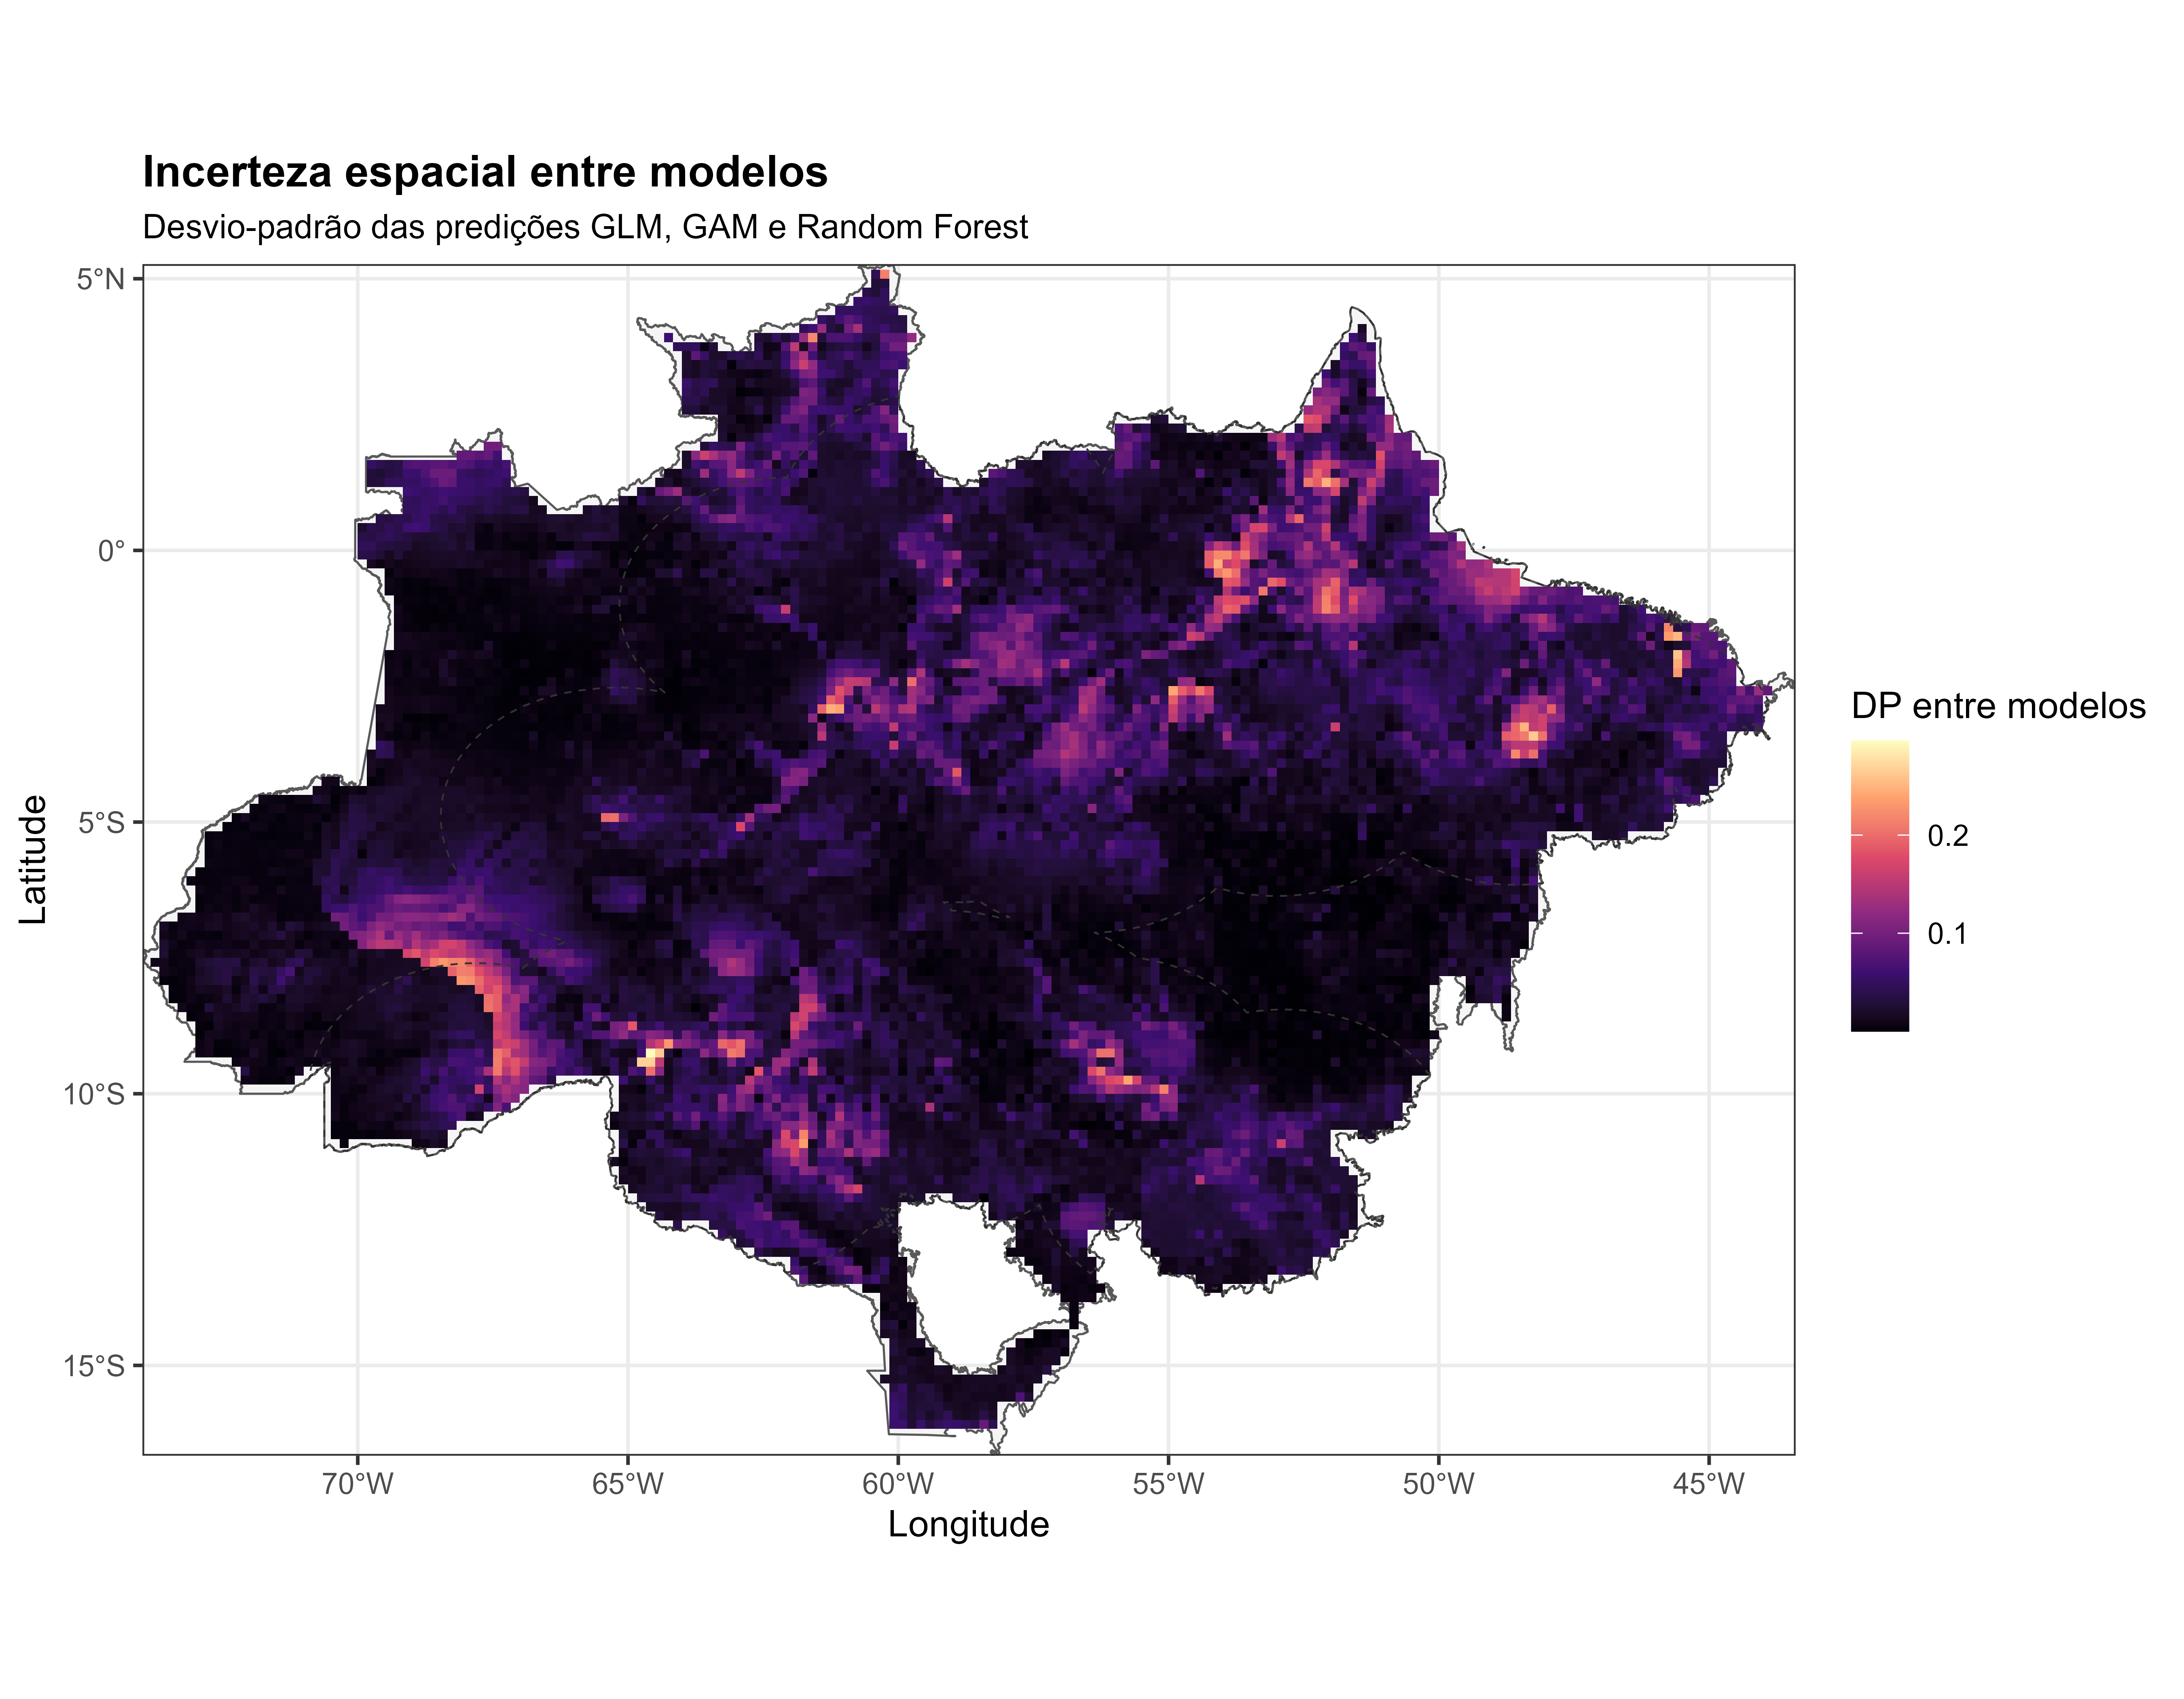
\includegraphics[width=0.78\textwidth]{figuras/unidade08/unidade08_incerteza_sd_glm_gam_rf.png}
  \caption{Spatial uncertainty measured as the standard deviation among GLM, GAM, and Random Forest predictions. High values indicate greater algorithmic disagreement; low values indicate stronger consensus.}
  \label{fig:unidade08_incerteza_modelos}
\end{figure}

\section{Partial Response Curves}

Partial dependence supports ecological interpretation. These curves are not
direct coefficients; they summarize the average prediction as one predictor
varies while the others are held constant.

\rscriptfile{scripts/unidade08/06_curvas_resposta_rf.R}

\begin{figure}[H]
  \centering
  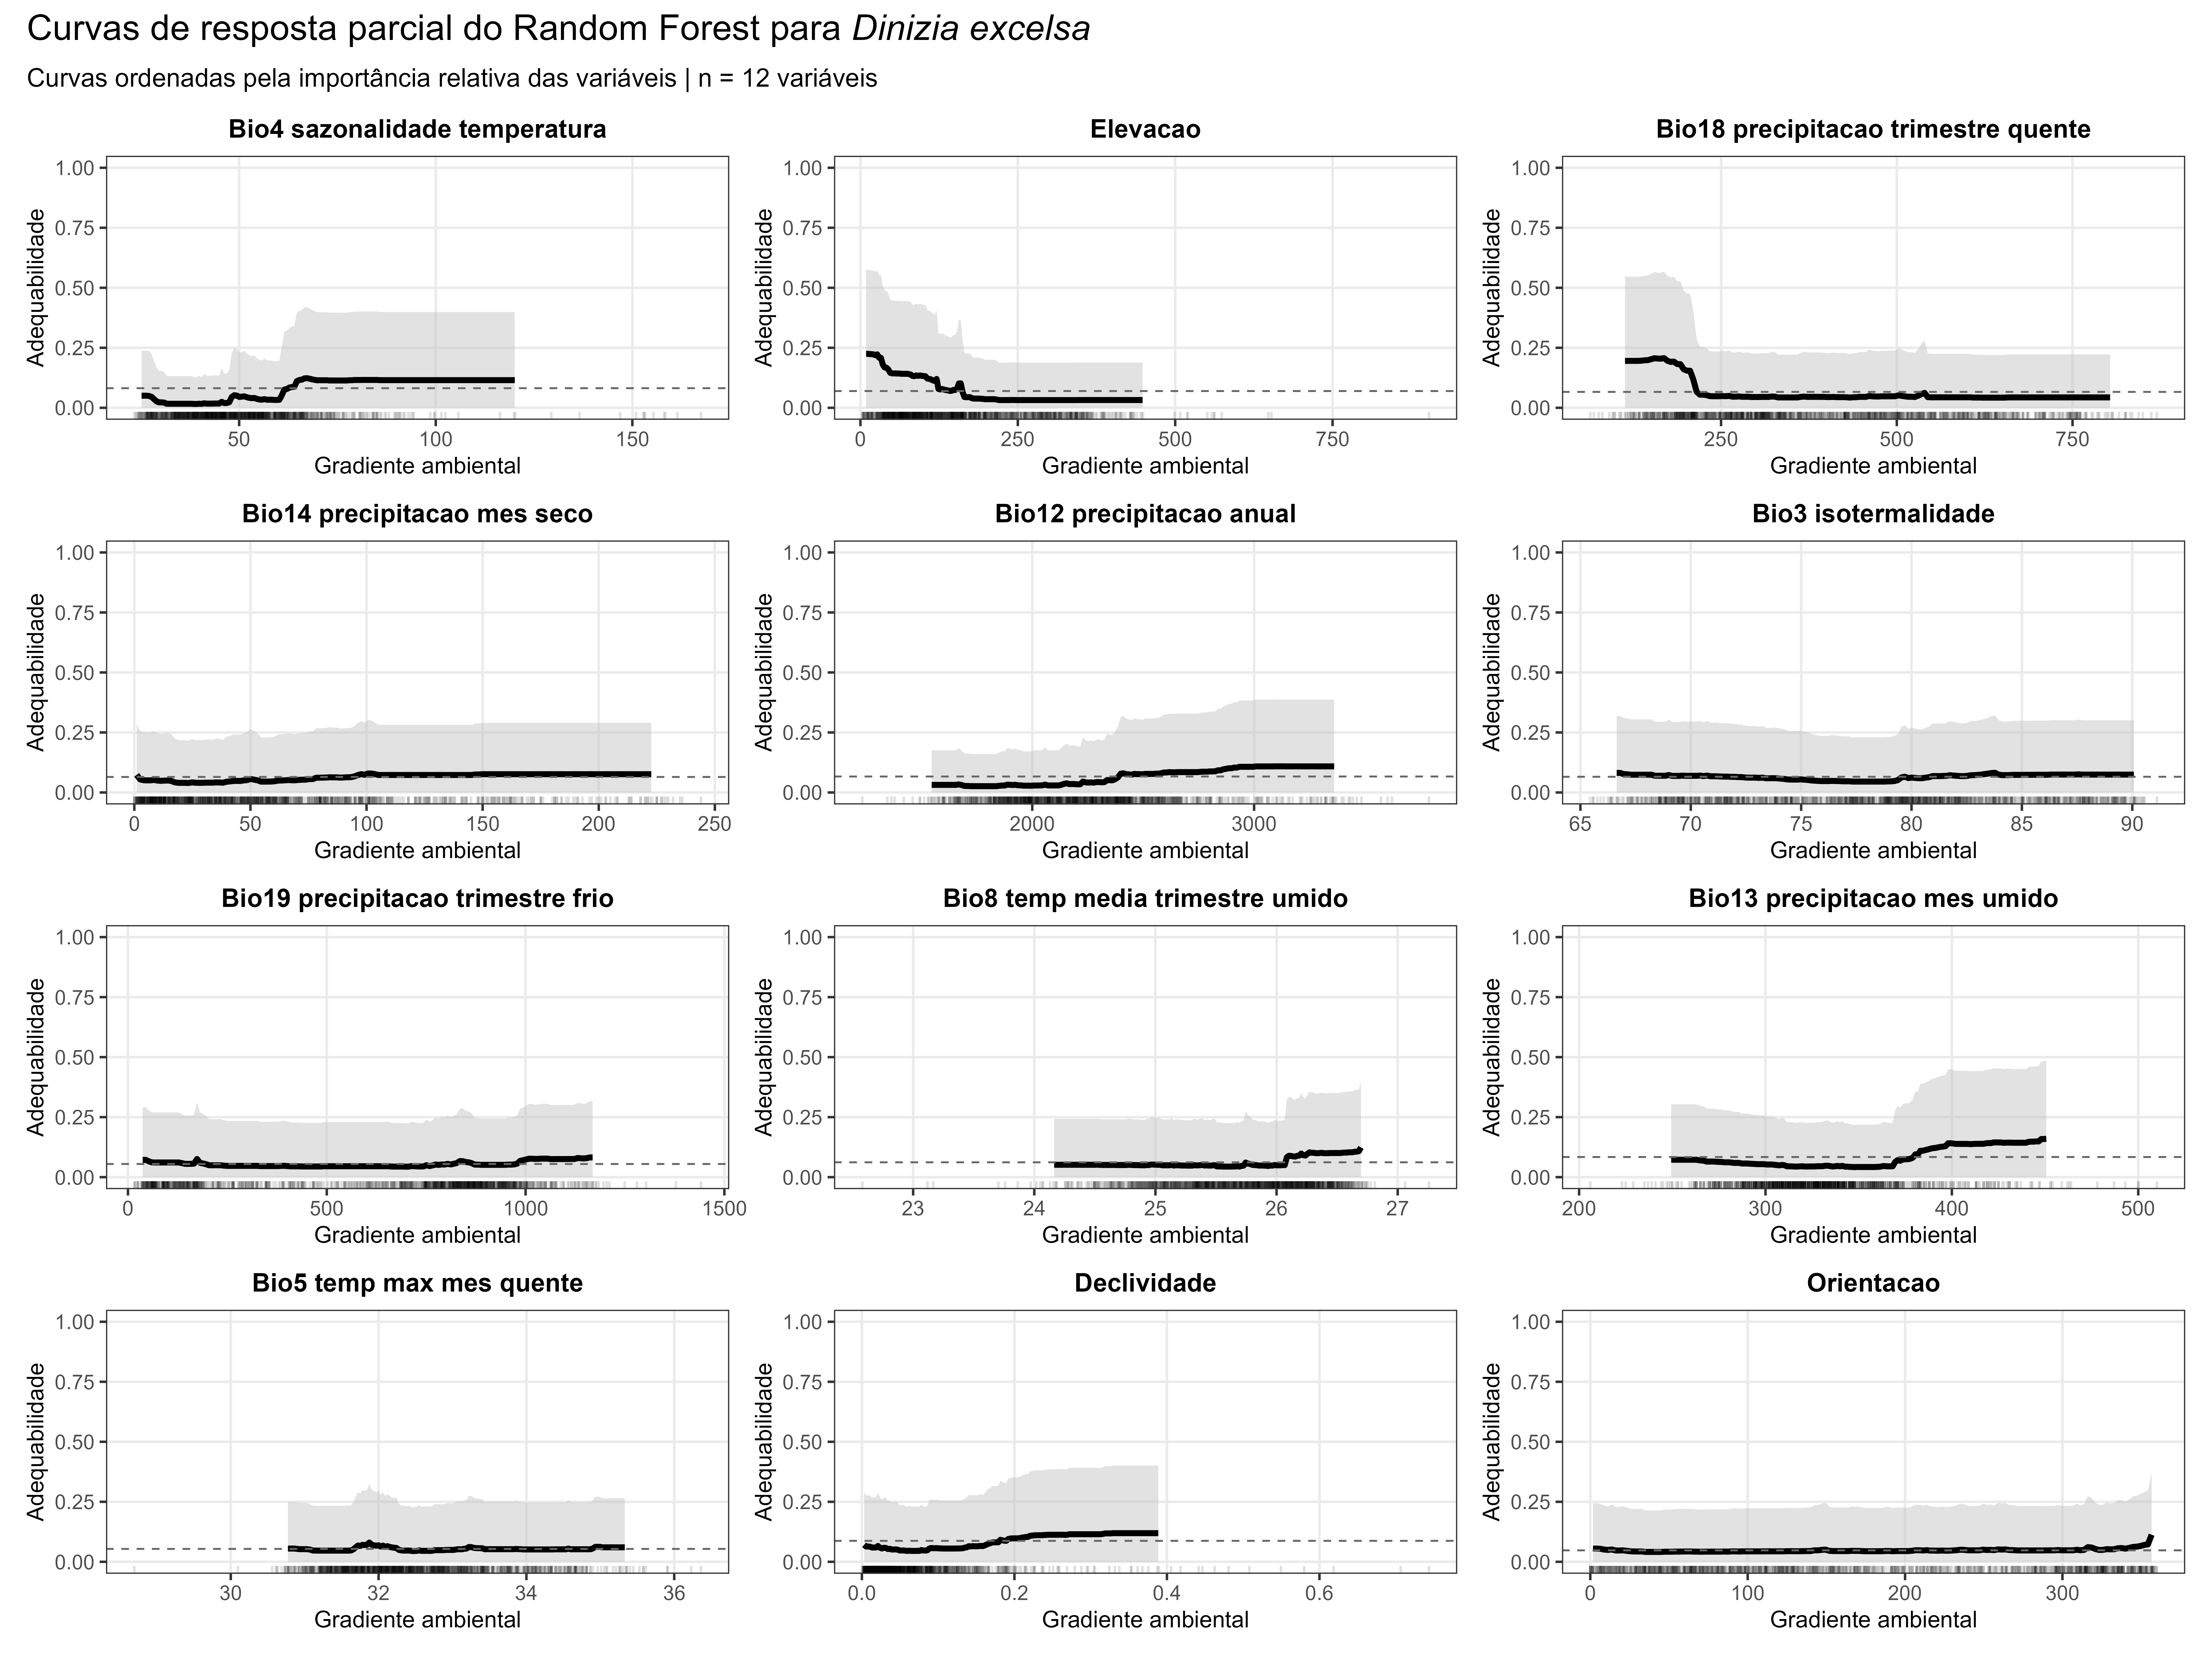
\includegraphics[width=0.96\textwidth]{figuras/unidade08/unidade08_curvas_resposta_rf.png}
  \caption{Random Forest partial response curves for the selected environmental predictors.}
  \label{fig:unidade08_curvas_resposta_rf}
\end{figure}

\section{Comparison with GLM and GAM}

The Random Forest map is compared with GLM and GAM projections, illustrating
how algorithms with different flexibility can produce distinct spatial patterns.

\rscriptfile{scripts/unidade08/07_comparar_glm_gam_rf.R}

\begin{figure}[H]
  \centering
  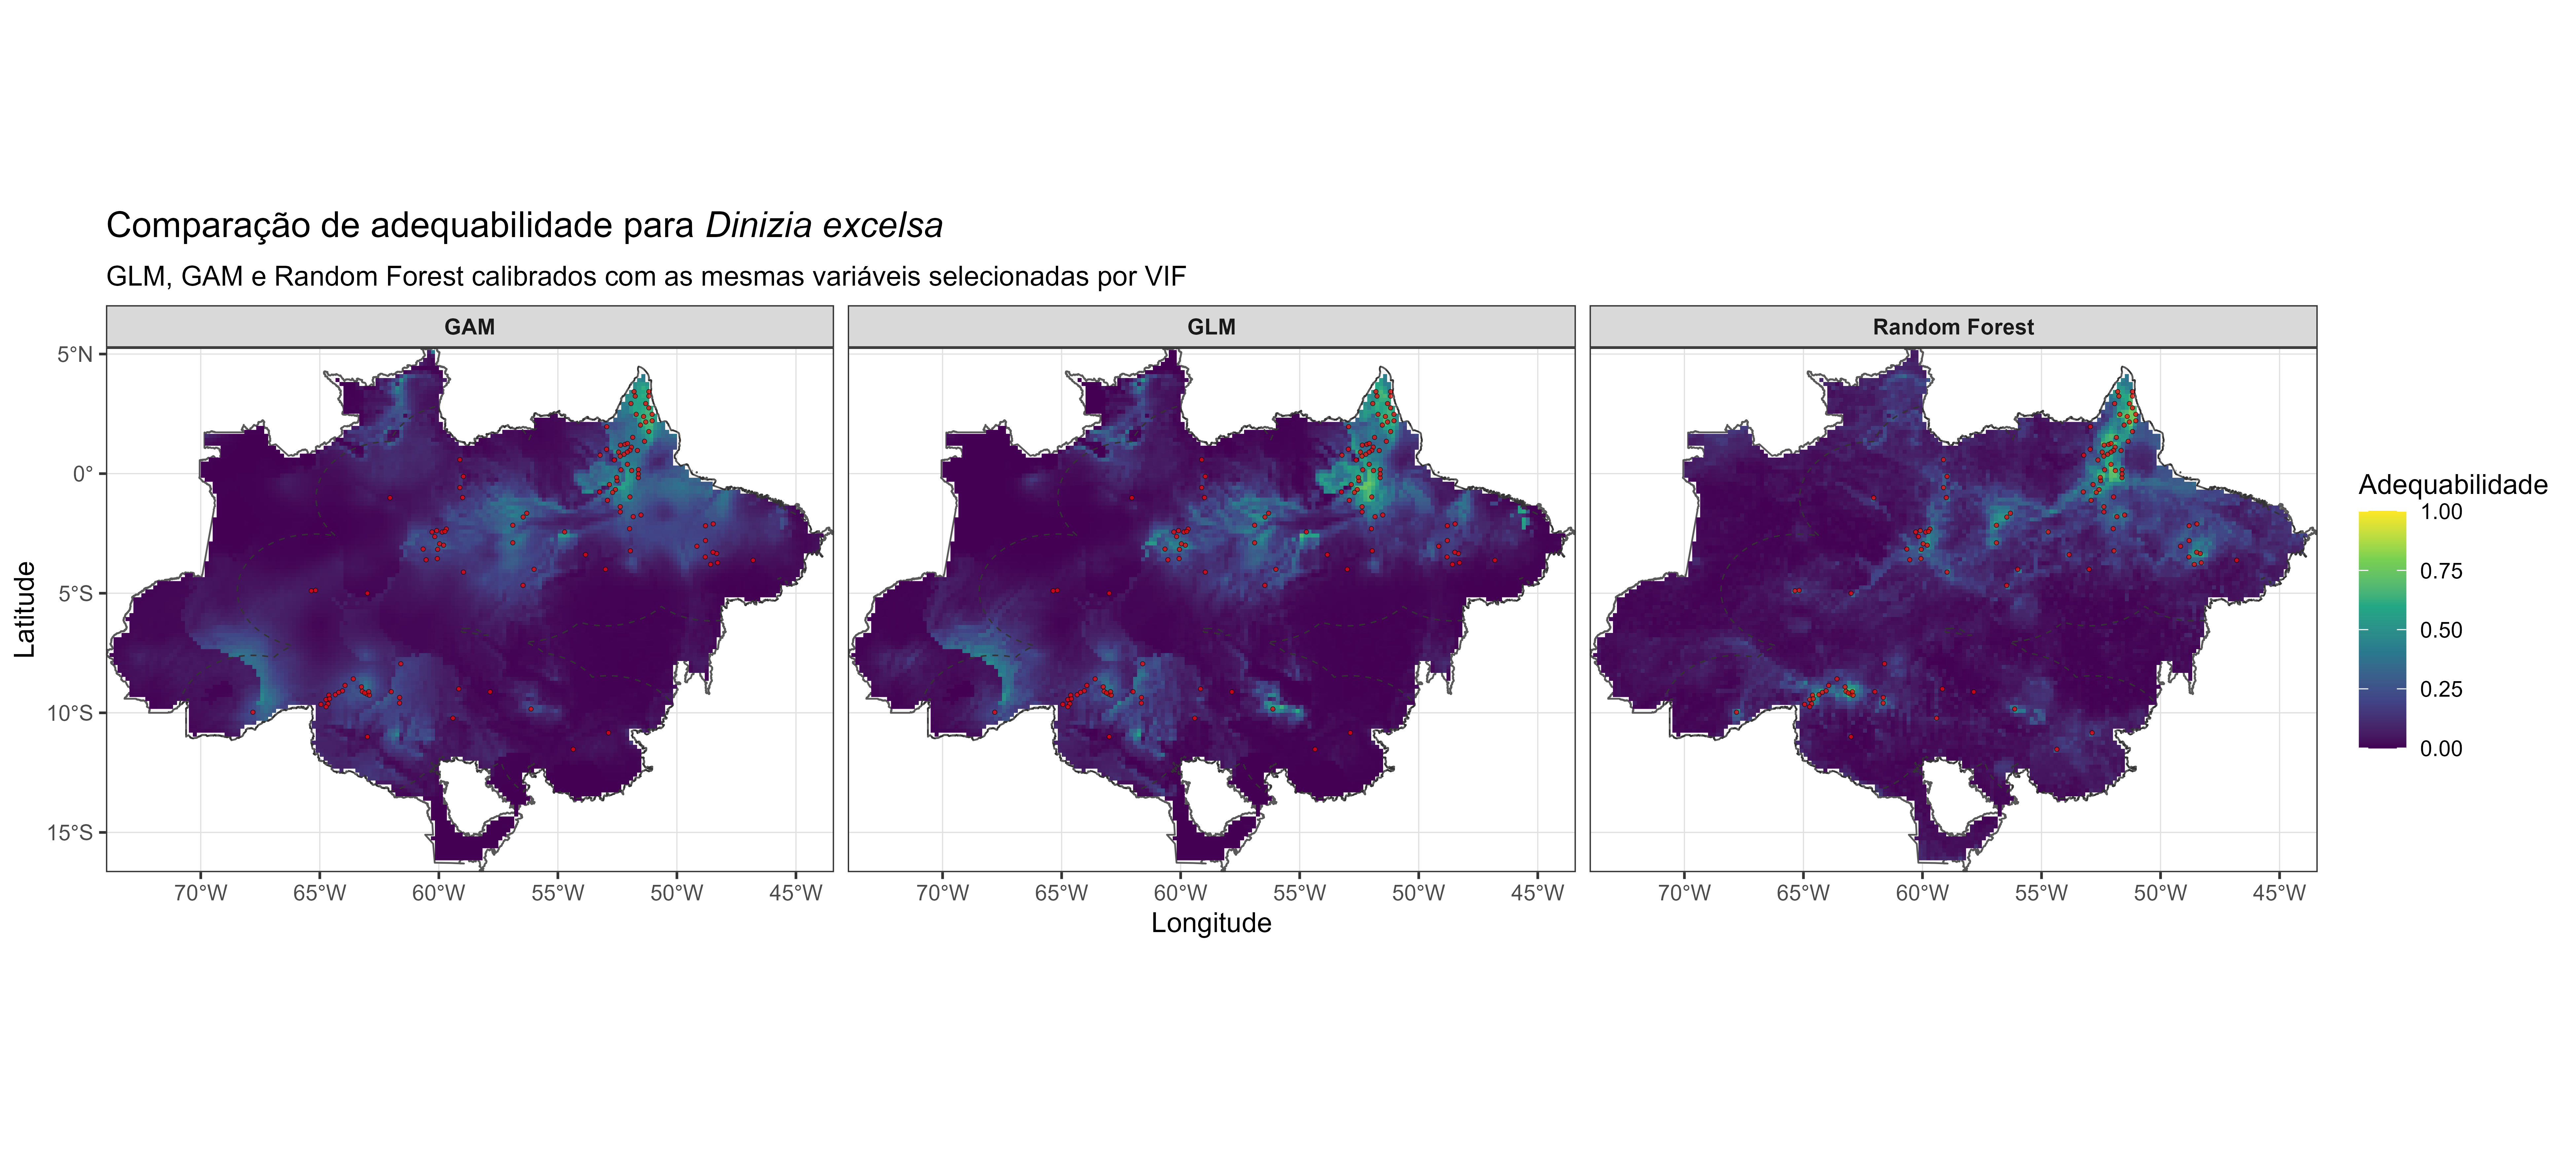
\includegraphics[width=0.96\textwidth]{figuras/unidade08/unidade08_comparacao_glm_gam_rf.png}
  \caption{Comparison of suitability maps estimated by GLM, GAM, and Random Forest.}
  \label{fig:unidade08_comparacao_modelos}
\end{figure}

\section{Complete Pipeline}
\rscriptfile{scripts/unidade08/08_pipeline_rf.R}

\section{Chapter Summary}

Random Forest is powerful when environmental relationships are nonlinear and
interactions are important. It nevertheless requires careful validation. High
metrics must be interpreted alongside overfitting diagnostics, ecological
coherence, response curves, spatial prediction patterns, and comparisons with
simpler models.

\begin{conceito}[title={\faBook\quad Key message}]
Random Forest may improve predictive performance, but it does not replace
ecological reasoning. A complex model is useful only when it generalizes,
produces plausible responses, and is evaluated independently.
\end{conceito}

\section{Review Exercises}
\begin{enumerate}
  \item Explain how Random Forest combines multiple decision trees.
  \item Why can Random Forest capture nonlinear relationships?
  \item What is overfitting in SDM?
  \item Why can an extremely high AUC be concerning?
  \item Distinguish OOB from test-set performance.
  \item What are the roles of \texttt{mtry}, \texttt{min.node.size}, and \texttt{sample.fraction}?
  \item How do partial response curves support interpretation of Random Forest?
\end{enumerate}

\chapter[BRT]{Boosted Regression Trees}

\begin{objetivos}
By the end of this chapter, readers should understand boosted regression trees
(BRTs); fit BRT presence--background models; control hyperparameters to reduce
overfitting; select the optimal number of trees by cross-validation; evaluate
models using AUC, TSS, sensitivity, and specificity; interpret relative
predictor importance and partial response curves; map suitability for
\textit{Dinizia excelsa}; and compare BRT with GLM, GAM, and Random Forest.
\end{objetivos}

\section{Introduction}

BRT combines decision trees with boosting. Unlike Random Forest, which fits
many largely independent trees and aggregates their predictions, boosting fits
trees sequentially so that each new tree improves residual errors from the
preceding ensemble. BRTs are widely used in SDM because they represent
nonlinear responses, predictor interactions, and complex environmental patterns
\parencite{elith2008working,elith2009,guisan2017habitat}.

\begin{conceito}[title={\faBook\quad BRT in SDM}]
BRT combines decision trees with sequential learning. It can represent complex
ecological relationships but requires careful hyperparameter control to avoid
overfitting.
\end{conceito}

\section{Main Hyperparameters}

The principal BRT hyperparameters are:
\begin{itemize}
  \item \texttt{n.trees}: maximum number of trees;
  \item \texttt{interaction.depth}: interaction complexity;
  \item \texttt{shrinkage}: learning rate;
  \item \texttt{bag.fraction}: fraction of observations used in each iteration; and
  \item \texttt{n.minobsinnode}: minimum observations in terminal nodes.
\end{itemize}

\begin{atencao}[title={\faExclamationTriangle\quad BRT and overfitting}]
BRT may overfit when the number of trees is excessive, the learning rate is
inappropriate, or trees are too deep. The optimal number of trees should be
selected by cross-validation.
\end{atencao}

\section{Data Preparation}
\rscriptfile{scripts/unidade09/01_estrutura_pastas.R}
\rscriptfile{scripts/unidade09/02_preparar_dados_brt.R}

\section{Fitting the BRT}

The BRT uses a Bernoulli distribution for binary presence--background data. The
optimal number of trees is selected using internal cross-validation.

\rscriptfile{scripts/unidade09/03_ajustar_brt_dinizia.R}

\begin{figure}[H]
  \centering
  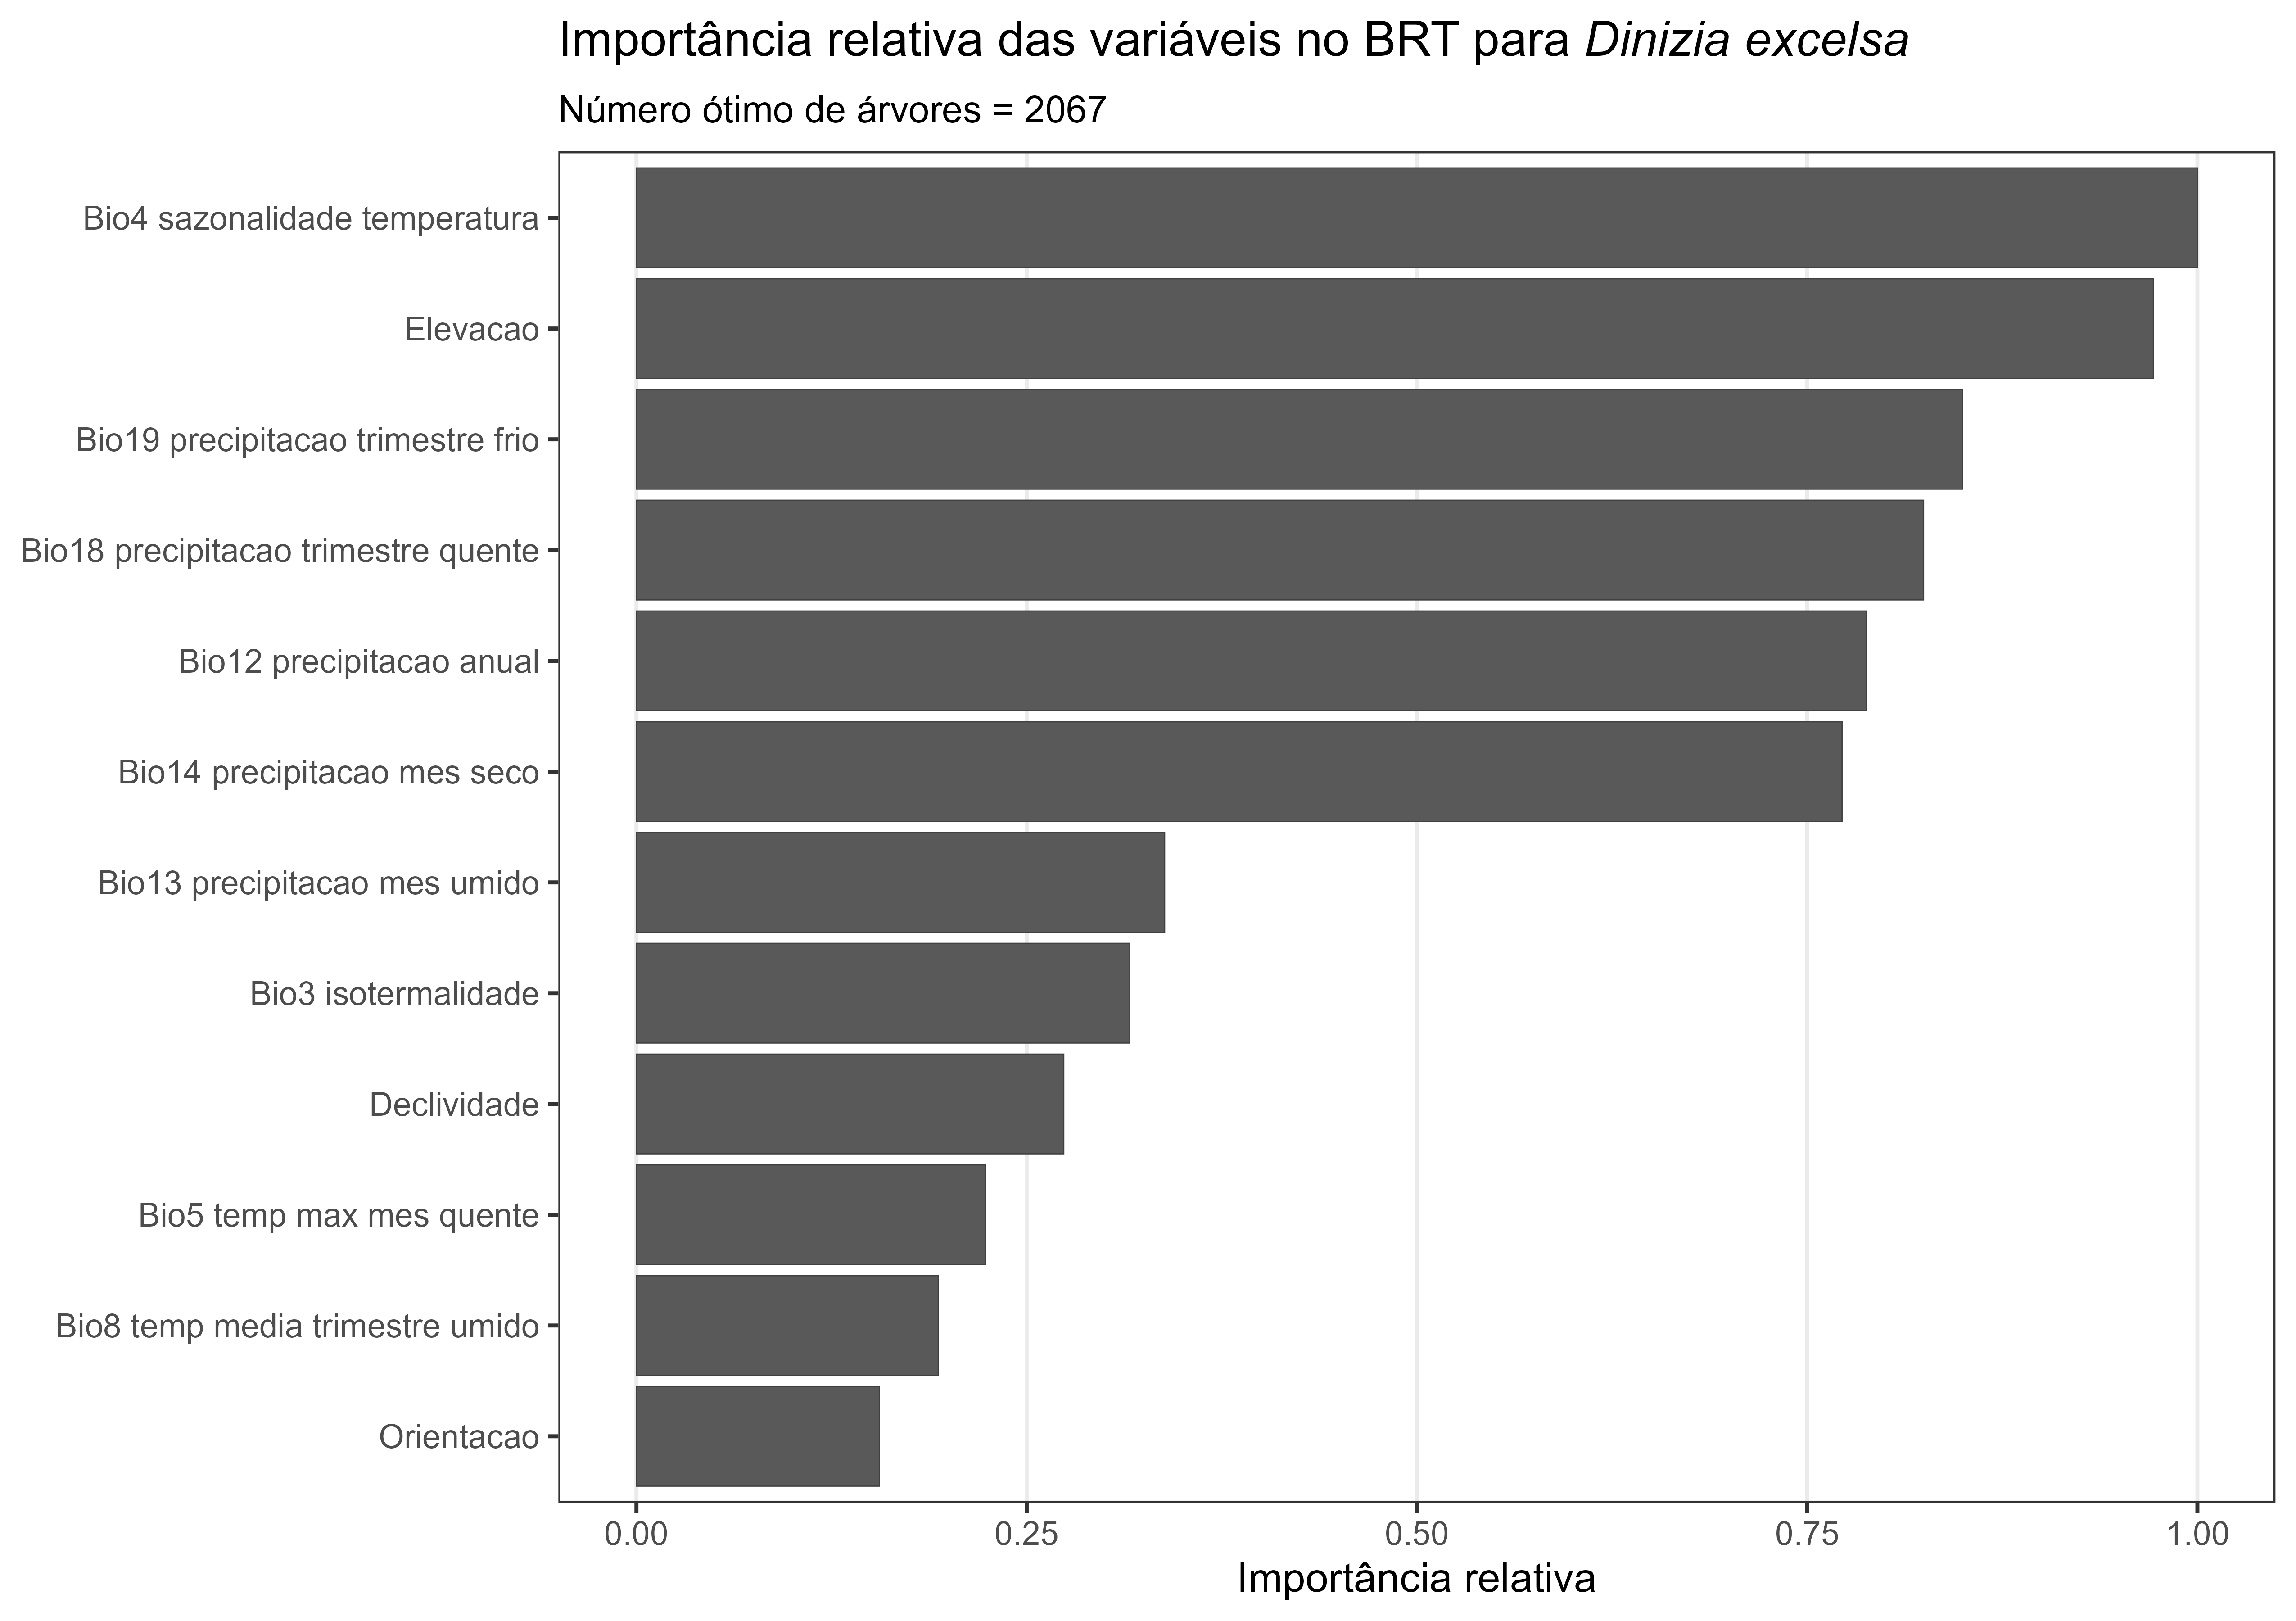
\includegraphics[width=0.86\textwidth]{figuras/unidade09/unidade09_importancia_variaveis_brt.png}
  \caption{Relative importance of environmental predictors in the BRT fitted to \textit{Dinizia excelsa}.}
  \label{fig:unidade09_importancia_brt}
\end{figure}

\section{Model Evaluation}
\rscriptfile{scripts/unidade09/04_avaliar_brt_dinizia.R}

\begin{figure}[H]
  \centering
  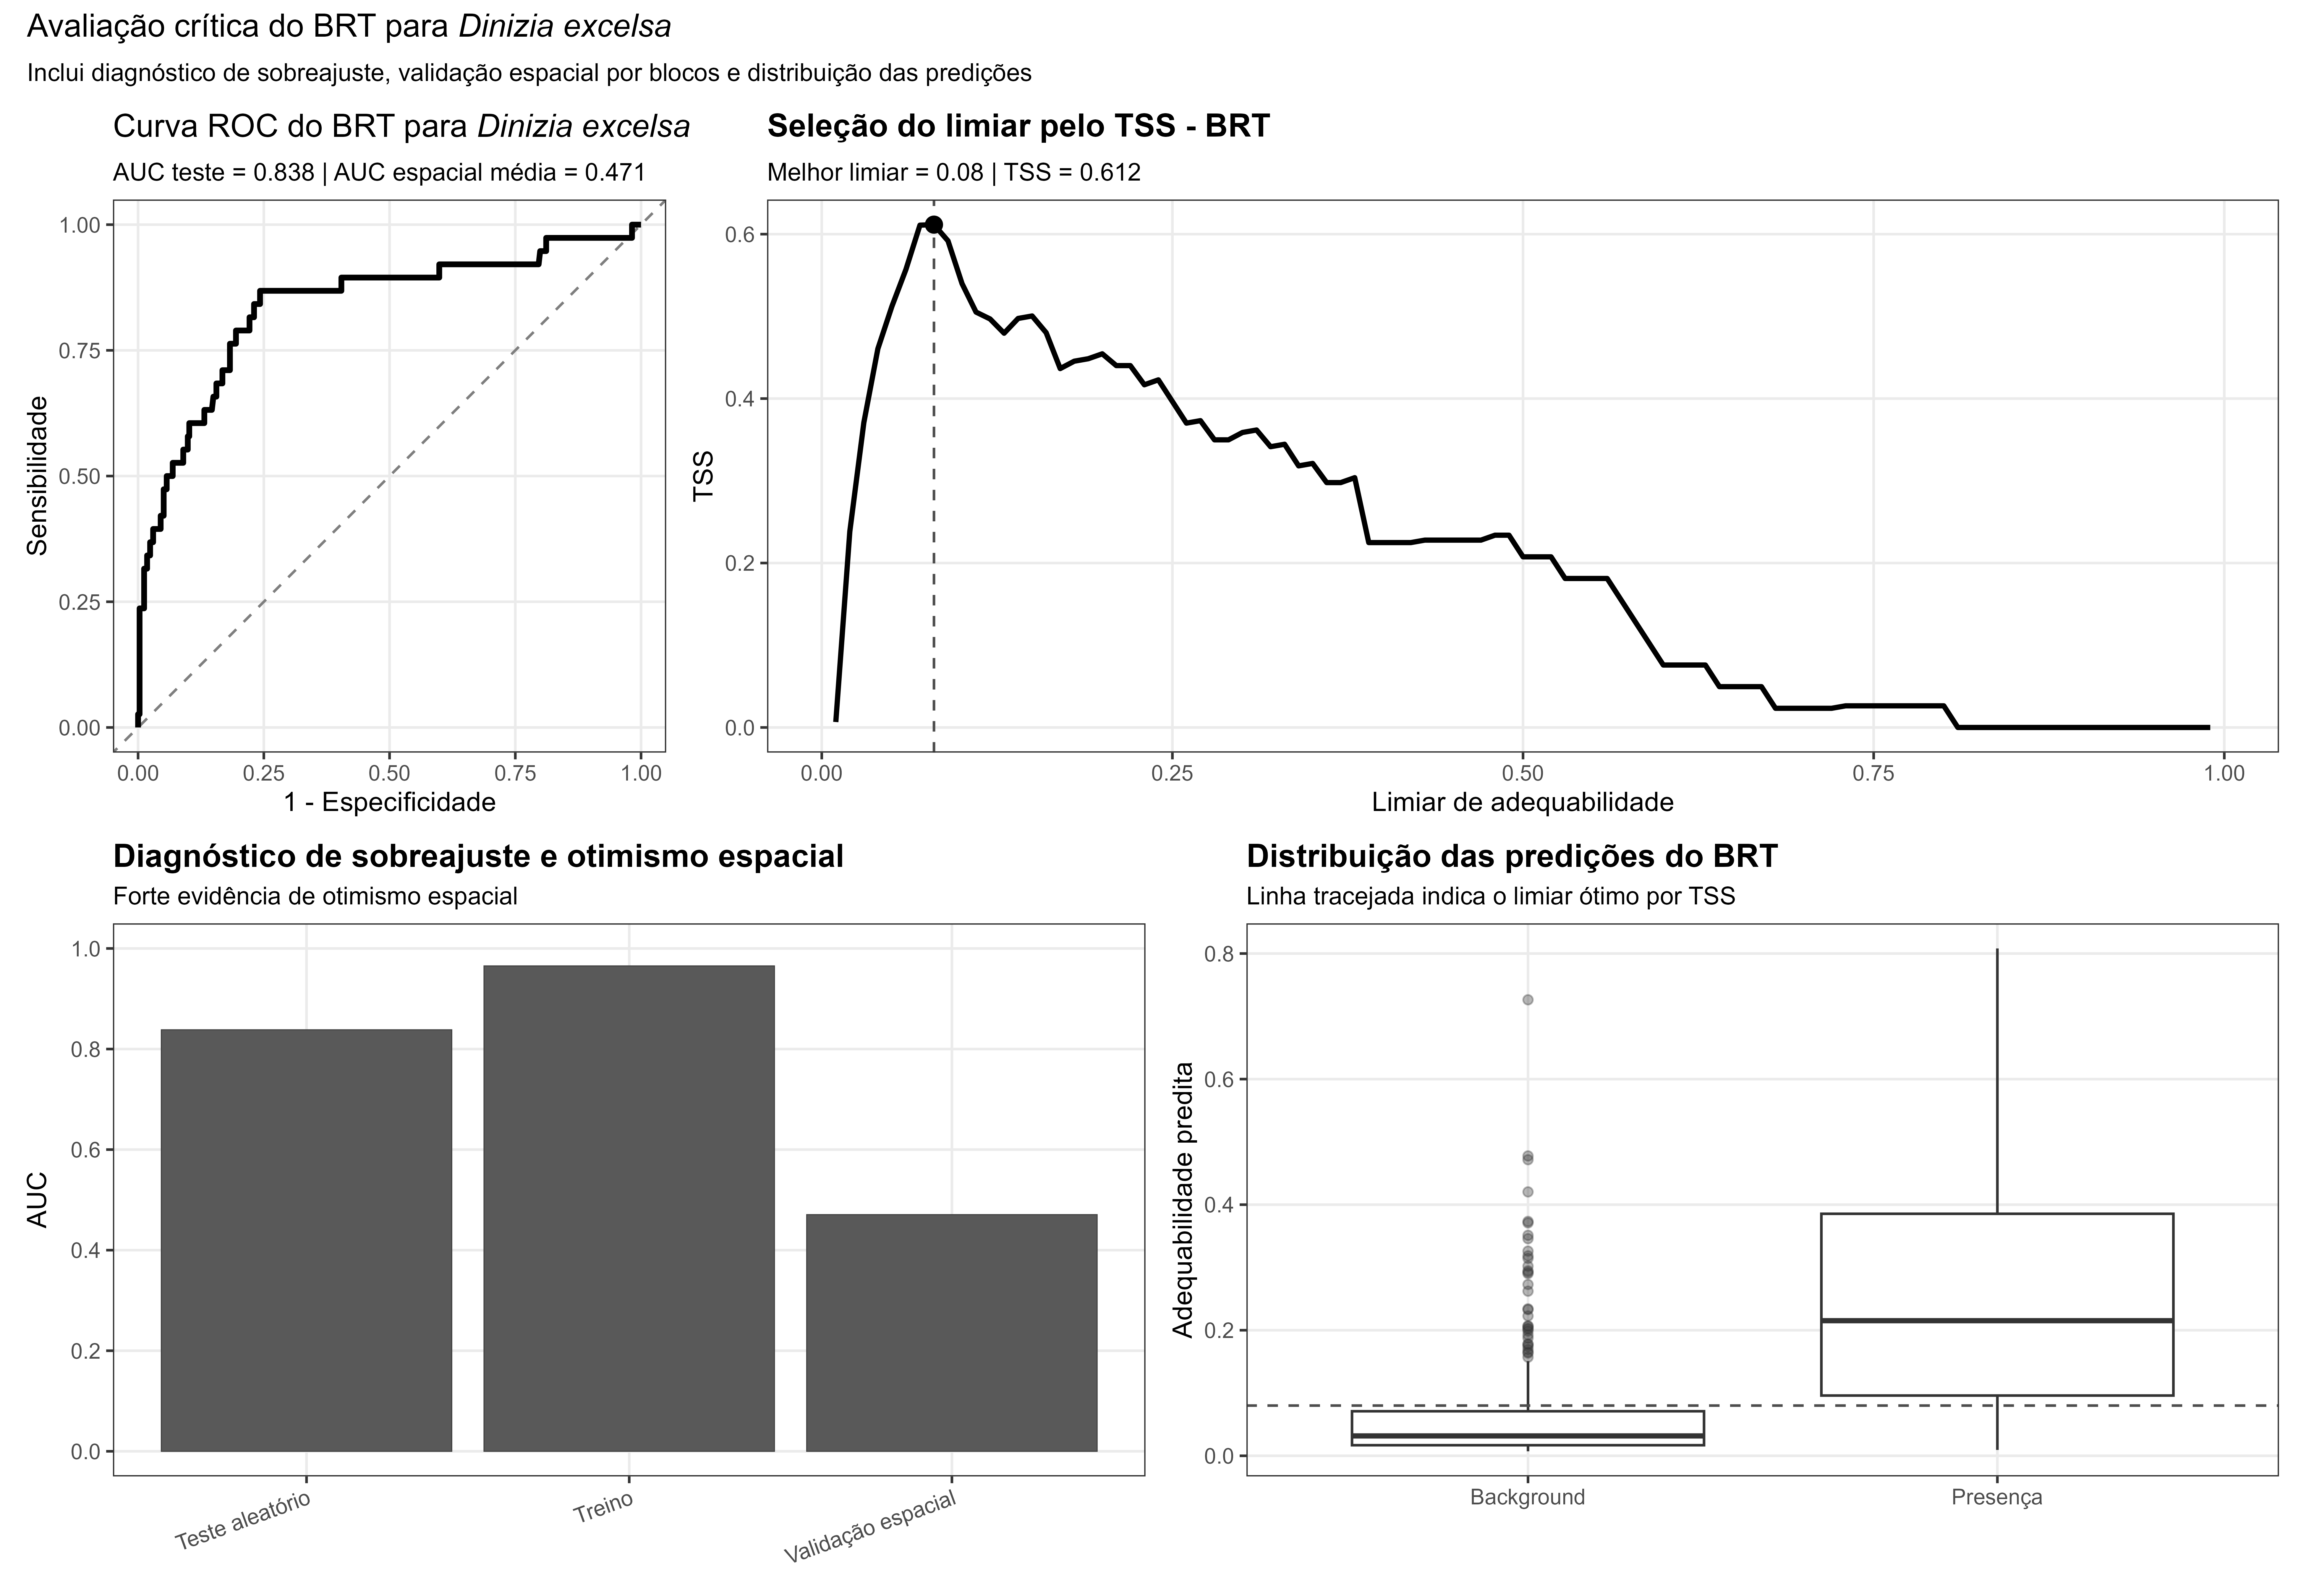
\includegraphics[width=0.78\textwidth]{figuras/unidade09/unidade09_avaliacao_brt_patchwork.png}
  \caption{ROC curve for the BRT evaluated on the test set.}
  \label{fig:unidade09_roc_brt}
\end{figure}

\begin{figure}[H]
  \centering
  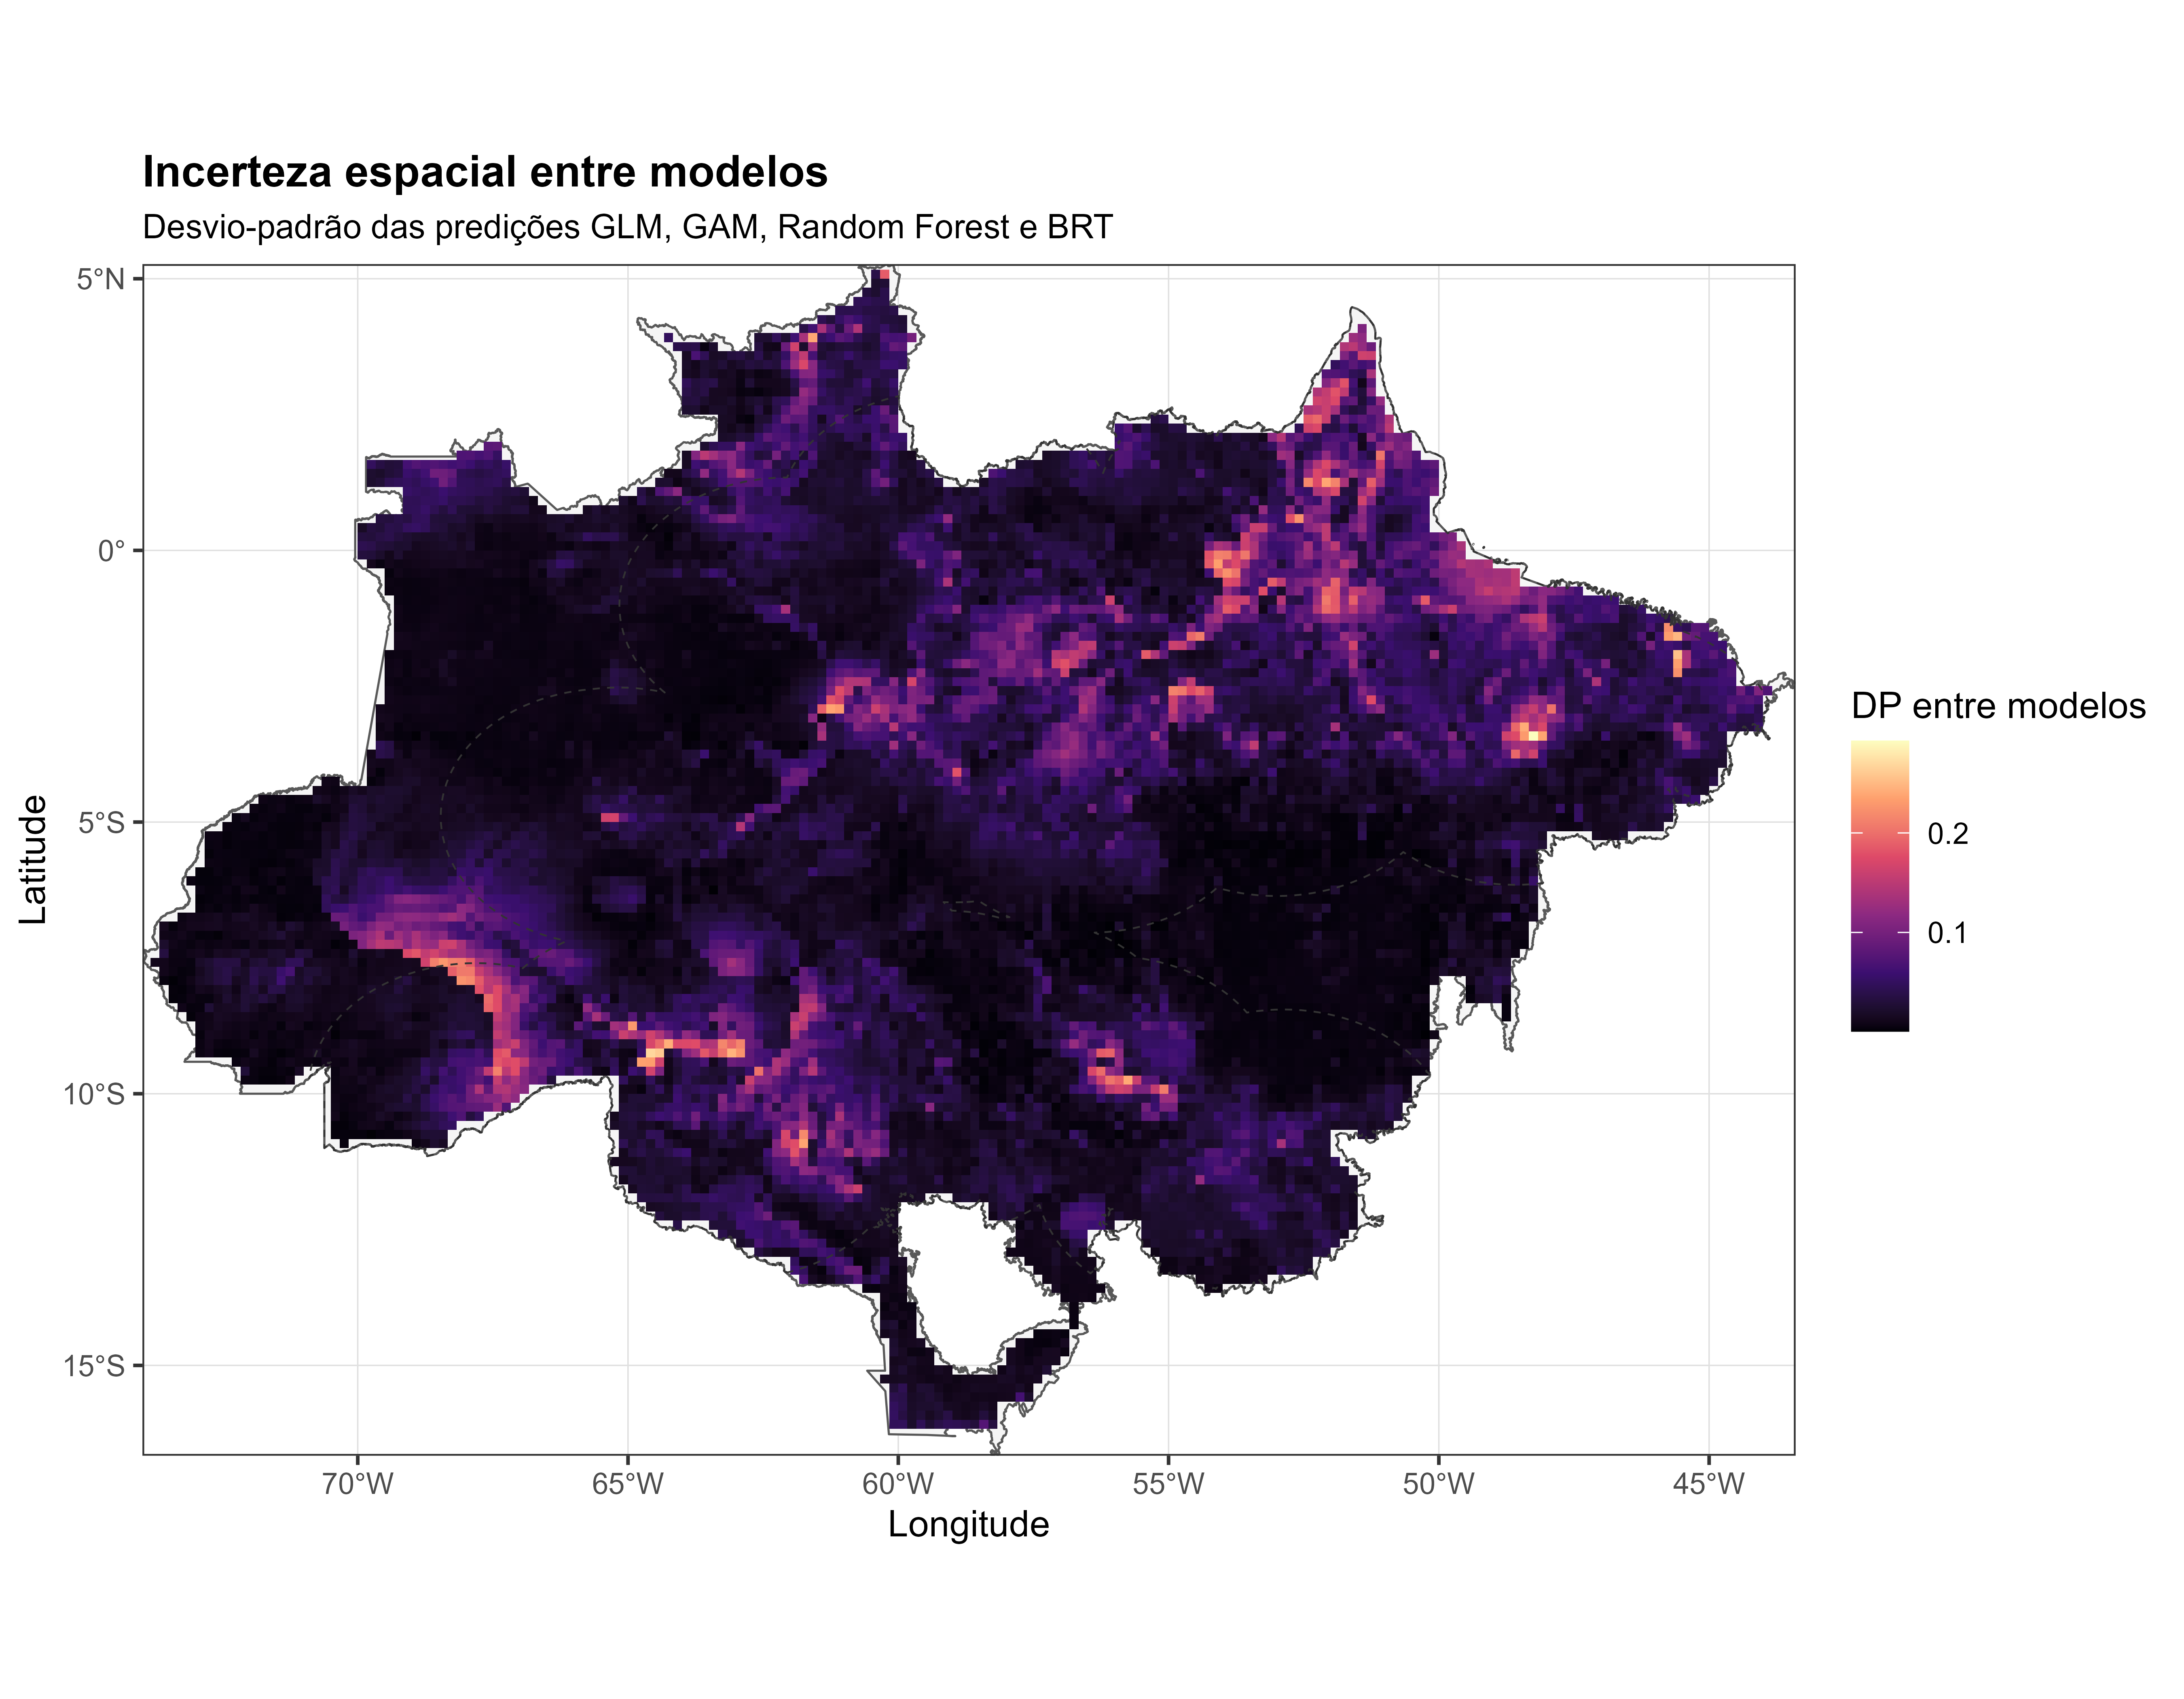
\includegraphics[width=0.78\textwidth]{figuras/unidade09/unidade09_incerteza_sd_glm_gam_rf_brt.png}
  \caption{Algorithmic disagreement for \textit{Dinizia excelsa}, calculated as the standard deviation among GLM, GAM, Random Forest, and BRT predictions. High values indicate weaker consensus among the fitted algorithms.}
  \label{fig:unidade09_incerteza_brt}
\end{figure}

\section{Current Suitability Map}
\rscriptfile{scripts/unidade09/05_predicao_espacial_brt.R}

\begin{figure}[H]
  \centering
  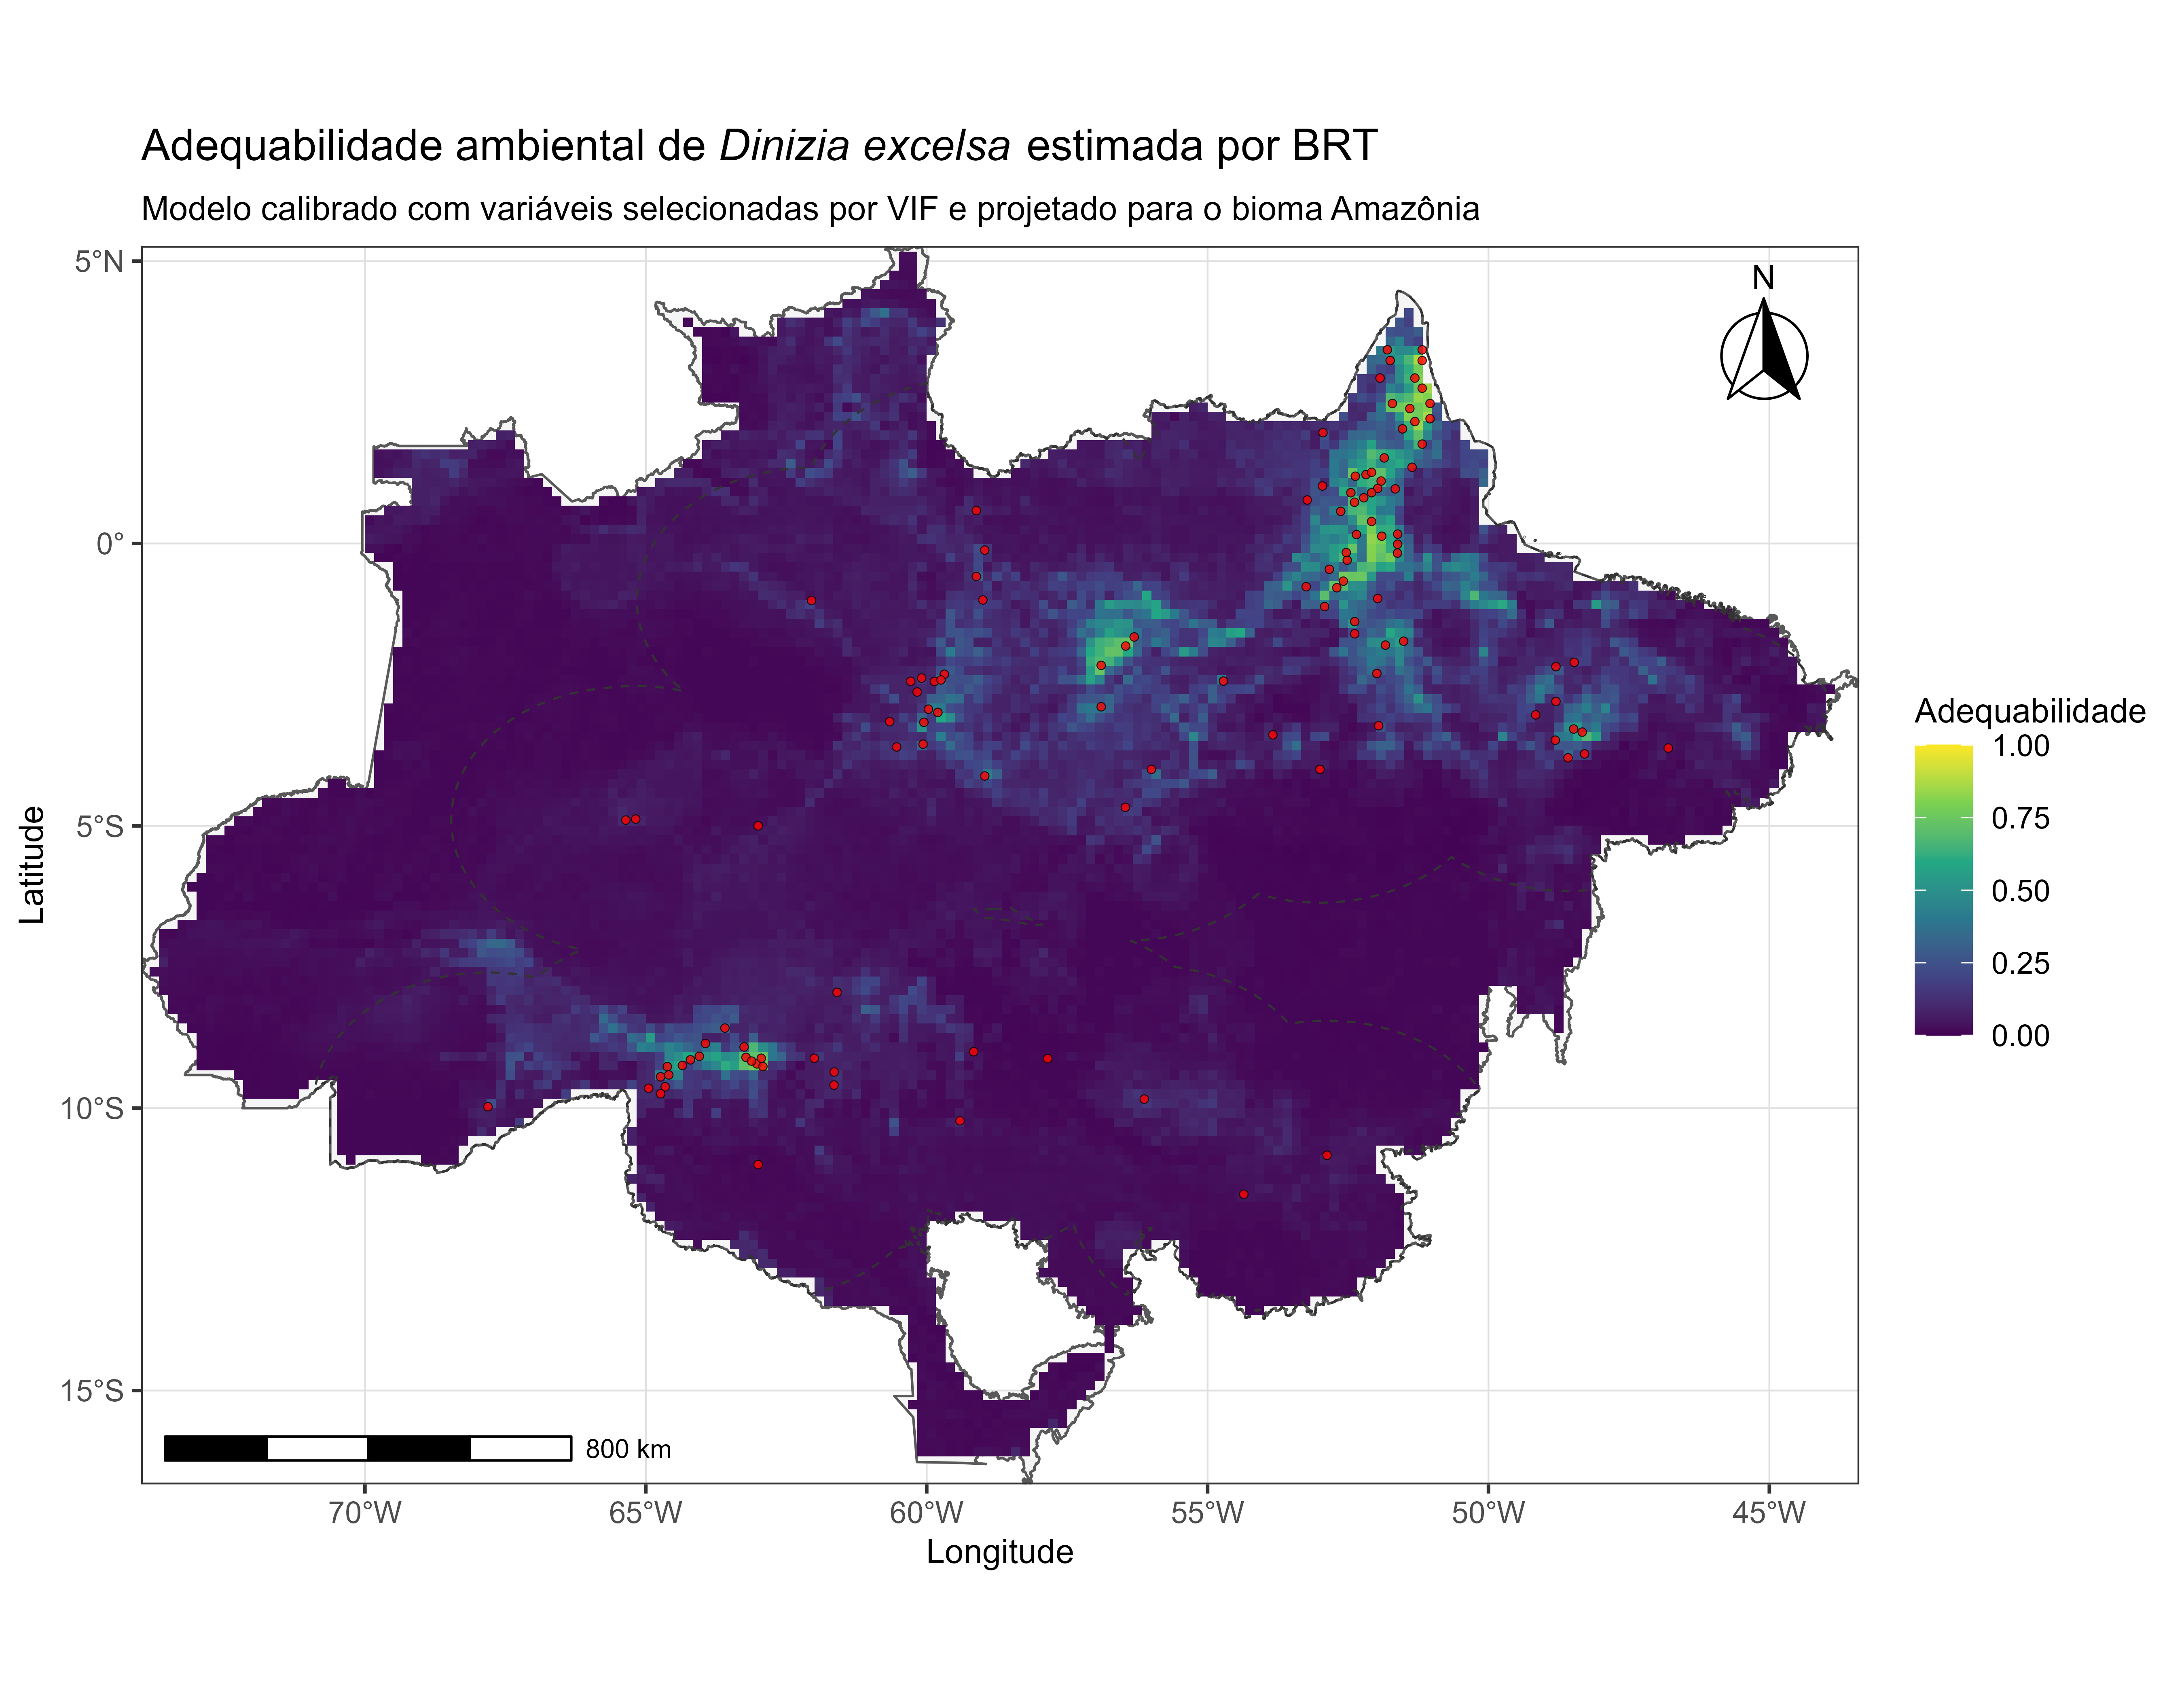
\includegraphics[width=0.88\textwidth]{figuras/unidade09/unidade09_adequabilidade_brt.png}
  \caption{Current suitability for \textit{Dinizia excelsa} estimated by BRT within the accessible area $M$.}
  \label{fig:unidade09_adequabilidade_brt}
\end{figure}

\section{Partial Response Curves}
\rscriptfile{scripts/unidade09/06_curvas_resposta_brt.R}

\begin{figure}[H]
  \centering
  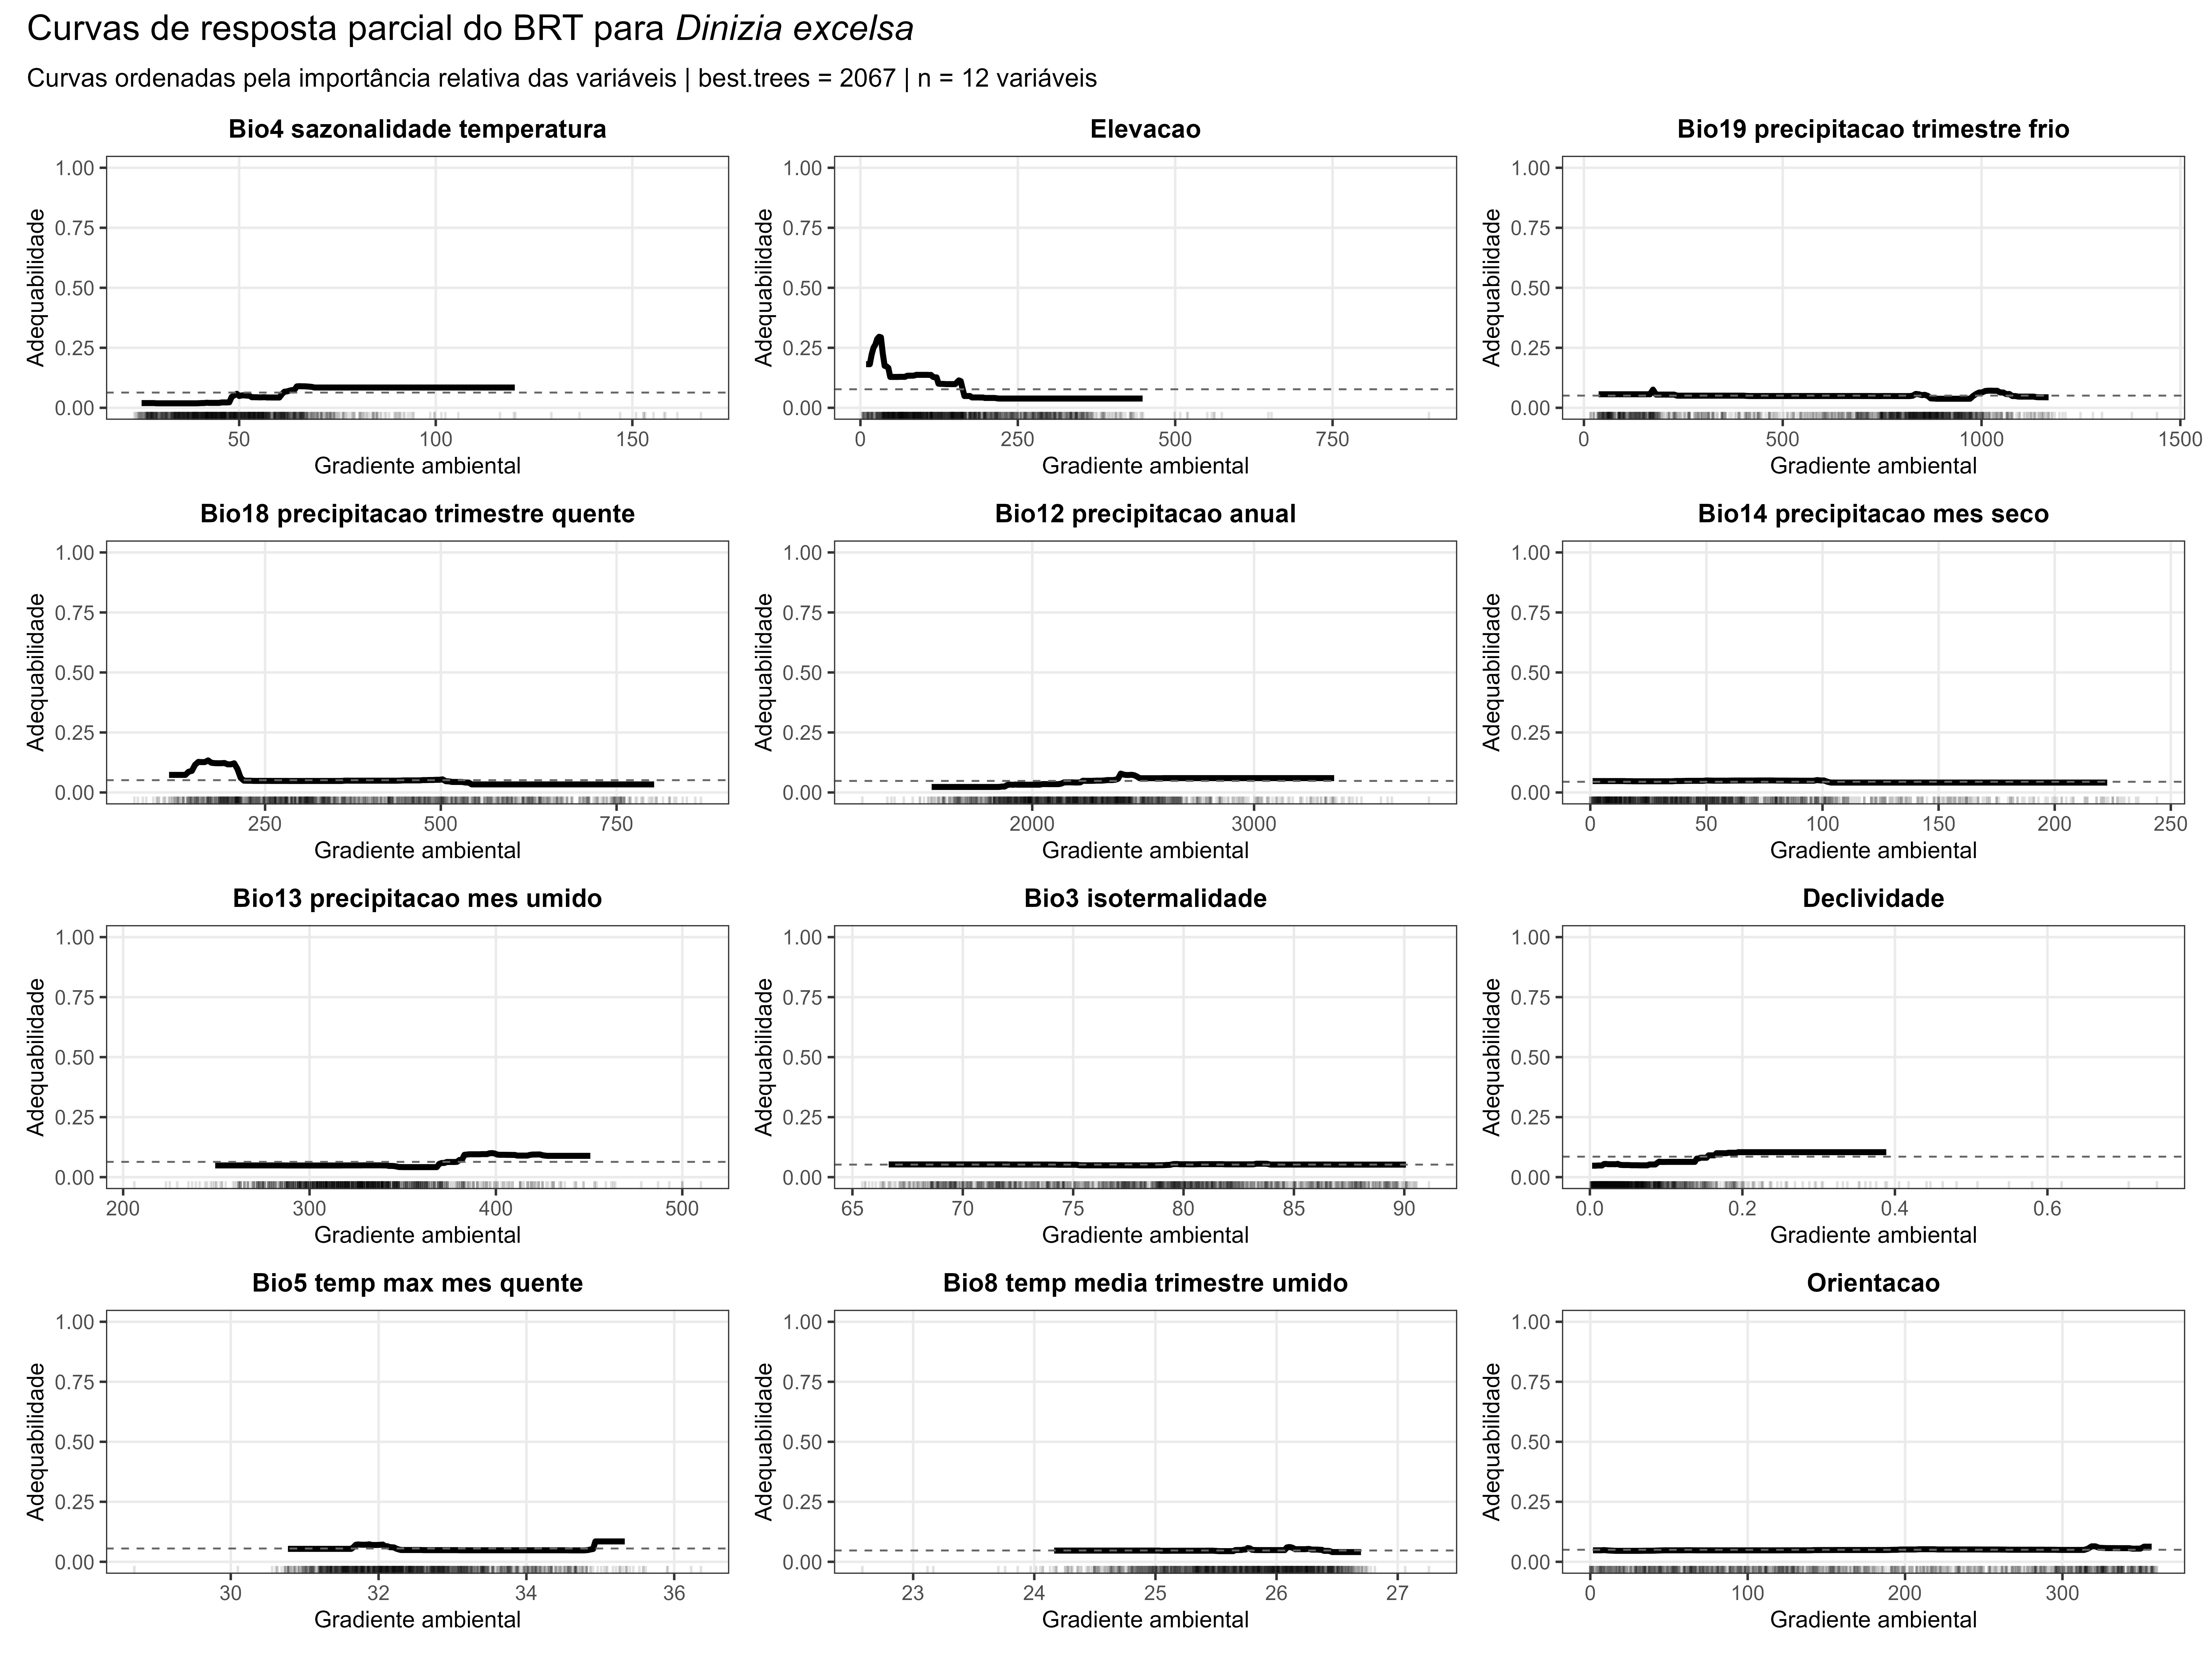
\includegraphics[width=0.96\textwidth]{figuras/unidade09/unidade09_curvas_resposta_brt.png}
  \caption{BRT partial response curves for the selected environmental predictors.}
  \label{fig:unidade09_curvas_resposta_brt}
\end{figure}

\section{Comparison with GLM, GAM, and Random Forest}
\rscriptfile{scripts/unidade09/07_comparar_modelos_brt.R}

\begin{figure}[H]
  \centering
  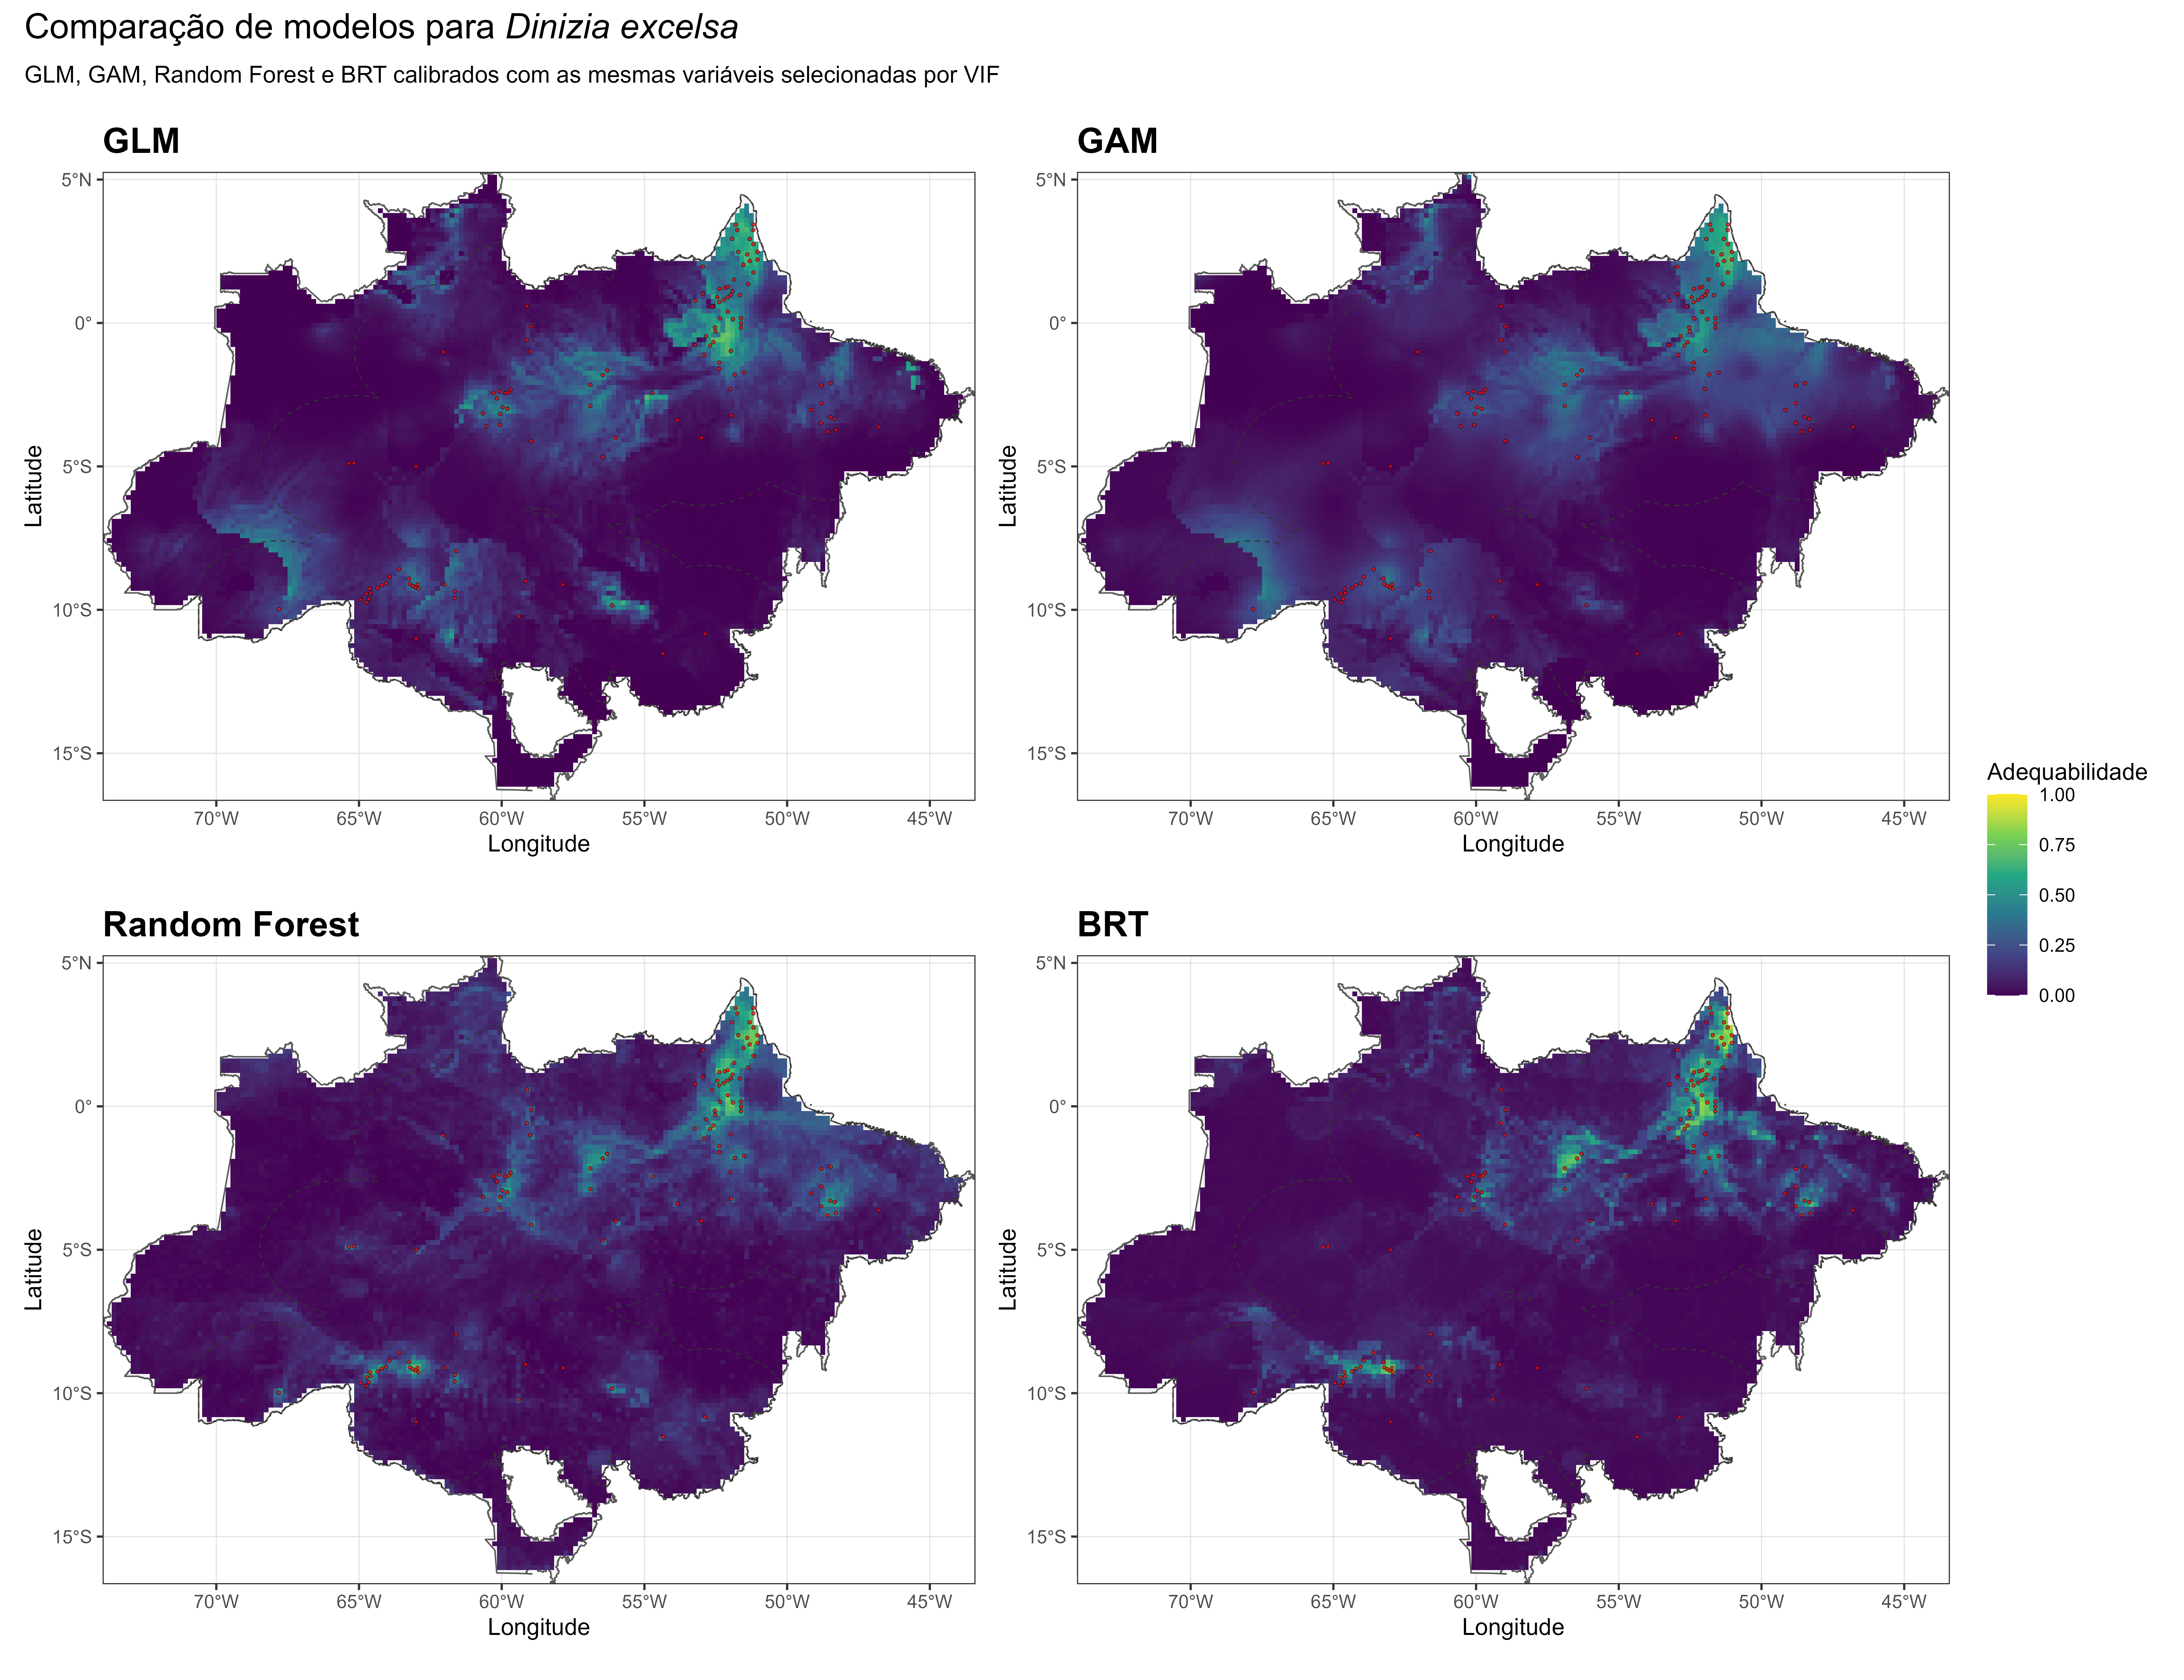
\includegraphics[width=0.96\textwidth]{figuras/unidade09/unidade09_comparacao_glm_gam_rf_brt.png}
  \caption{Comparison of suitability maps estimated by GLM, GAM, Random Forest, and BRT.}
  \label{fig:unidade09_comparacao_modelos}
\end{figure}

\section{Complete Pipeline}
\rscriptfile{scripts/unidade09/08_pipeline_brt.R}

\section{Chapter Summary}

BRT combines flexibility, interactions, and strong predictive performance, but
requires careful hyperparameter control and evaluation with independent data.

\begin{conceito}[title={\faBook\quad Key message}]
BRT can reveal complex environmental responses, but its credibility depends on
appropriate validation, overfitting control, and ecological interpretation.
\end{conceito}

\section{Review Exercises}
\begin{enumerate}
  \item Explain the difference between Random Forest and BRT.
  \item What does boosting mean?
  \item Why is \texttt{shrinkage} important?
  \item What is the role of \texttt{interaction.depth}?
  \item Why should cross-validation select the optimal number of trees?
  \item How is relative predictor importance interpreted in BRT?
  \item Why should partial response curves be evaluated critically?
\end{enumerate}

\chapter[Maxent]{Maximum Entropy}

\begin{objetivos}
By the end of this chapter, readers should understand Maxent and the maximum
entropy principle; distinguish linear, quadratic, product, hinge, and threshold
features; explain regularization; fit Maxent to \textit{Dinizia excelsa}
presence--background data; tune feature classes and the regularization
multiplier; evaluate performance independently; generate response curves and a
current suitability map; and compare Maxent with GLM, GAM, Random Forest, and BRT.
\end{objetivos}

\section{Introduction}

Maxent is among the most widely used SDM methods, especially when available data
consist of presences and background. It estimates a maximum-entropy
distribution---the most uniform distribution possible subject to constraints
imposed by environmental conditions at presence sites
\parencite{phillips2006maximum,phillips2008modeling,elith2011statistical,merow2013practical,guisan2017habitat}.

In practice, Maxent contrasts environmental values at presences with those
available in the background. It estimates a relative-suitability function that
identifies combinations resembling conditions where the species was observed.

\begin{conceito}[title={\faBook\quad Maxent in SDM}]
Maxent is a presence--background method based on maximum entropy. It estimates
a spatial distribution satisfying environmental constraints observed at
presences without assuming more structure than the available information supports.
\end{conceito}

\section{Maximum Entropy and Environmental Suitability}

Maximum entropy seeks the least biased distribution consistent with specified
constraints. In SDM, constraints derive from environmental variables at
presence locations.

\begin{equationbox}
\[
\hat{p}(x)=\frac{\exp\left(\sum_j\lambda_j f_j(x)\right)}{Z}.
\]
\end{equationbox}

Here, $\hat p(x)$ is relative suitability at location $x$, $f_j(x)$ are
functions of environmental predictors, $\lambda_j$ are estimated weights, and
$Z$ is a normalizing constant.

\section{Feature Classes}

Maxent represents species--environment relationships through feature classes:
\begin{itemize}
  \item linear (L): linear responses;
  \item quadratic (Q): unimodal or parabolic responses;
  \item product (P): interactions among predictors;
  \item hinge (H): piecewise responses and thresholds; and
  \item threshold (T): responses based on discrete cutoffs.
\end{itemize}

\begin{atencao}[title={\faExclamationTriangle\quad Maxent complexity}]
Many features combined with weak regularization can overfit. Feature classes and
regularization must therefore be tuned and evaluated outside calibration data.
\end{atencao}

\section{Regularization}

Regularization controls model complexity. Low values allow flexible responses
but increase overfitting risk. High values yield simpler, smoother models but
may fail to capture genuine ecological structure. The main tuning parameter is
the \textit{regularization multiplier}.

\begin{conceito}[title={\faBook\quad Regularization}]
Regularization penalizes excessive complexity. It is essential for spatial and
temporal transferability, particularly in future or paleoclimatic projections.
\end{conceito}

\section{Data Preparation}

The model uses the Chapter 5 presence--background dataset and Chapter 4
predictors. It is fitted with \texttt{maxnet}, an R implementation of penalized
Maxent that does not require \texttt{maxent.jar}.

\rscriptfile{scripts/unidade10/01_estrutura_pastas.R}
\rscriptfile{scripts/unidade10/02_preparar_dados_maxent.R}

\section{Tuning Feature Classes and Regularization}

Tuning compares feature-class combinations and regularization multipliers to
select a model with useful predictive performance but without unnecessary
complexity. Selection must be based on a prespecified criterion and data not
used to optimize the fitted coefficients.

\rscriptfile{scripts/unidade10/03_tuning_maxent_dinizia.R}

\begin{figure}[H]
  \centering
  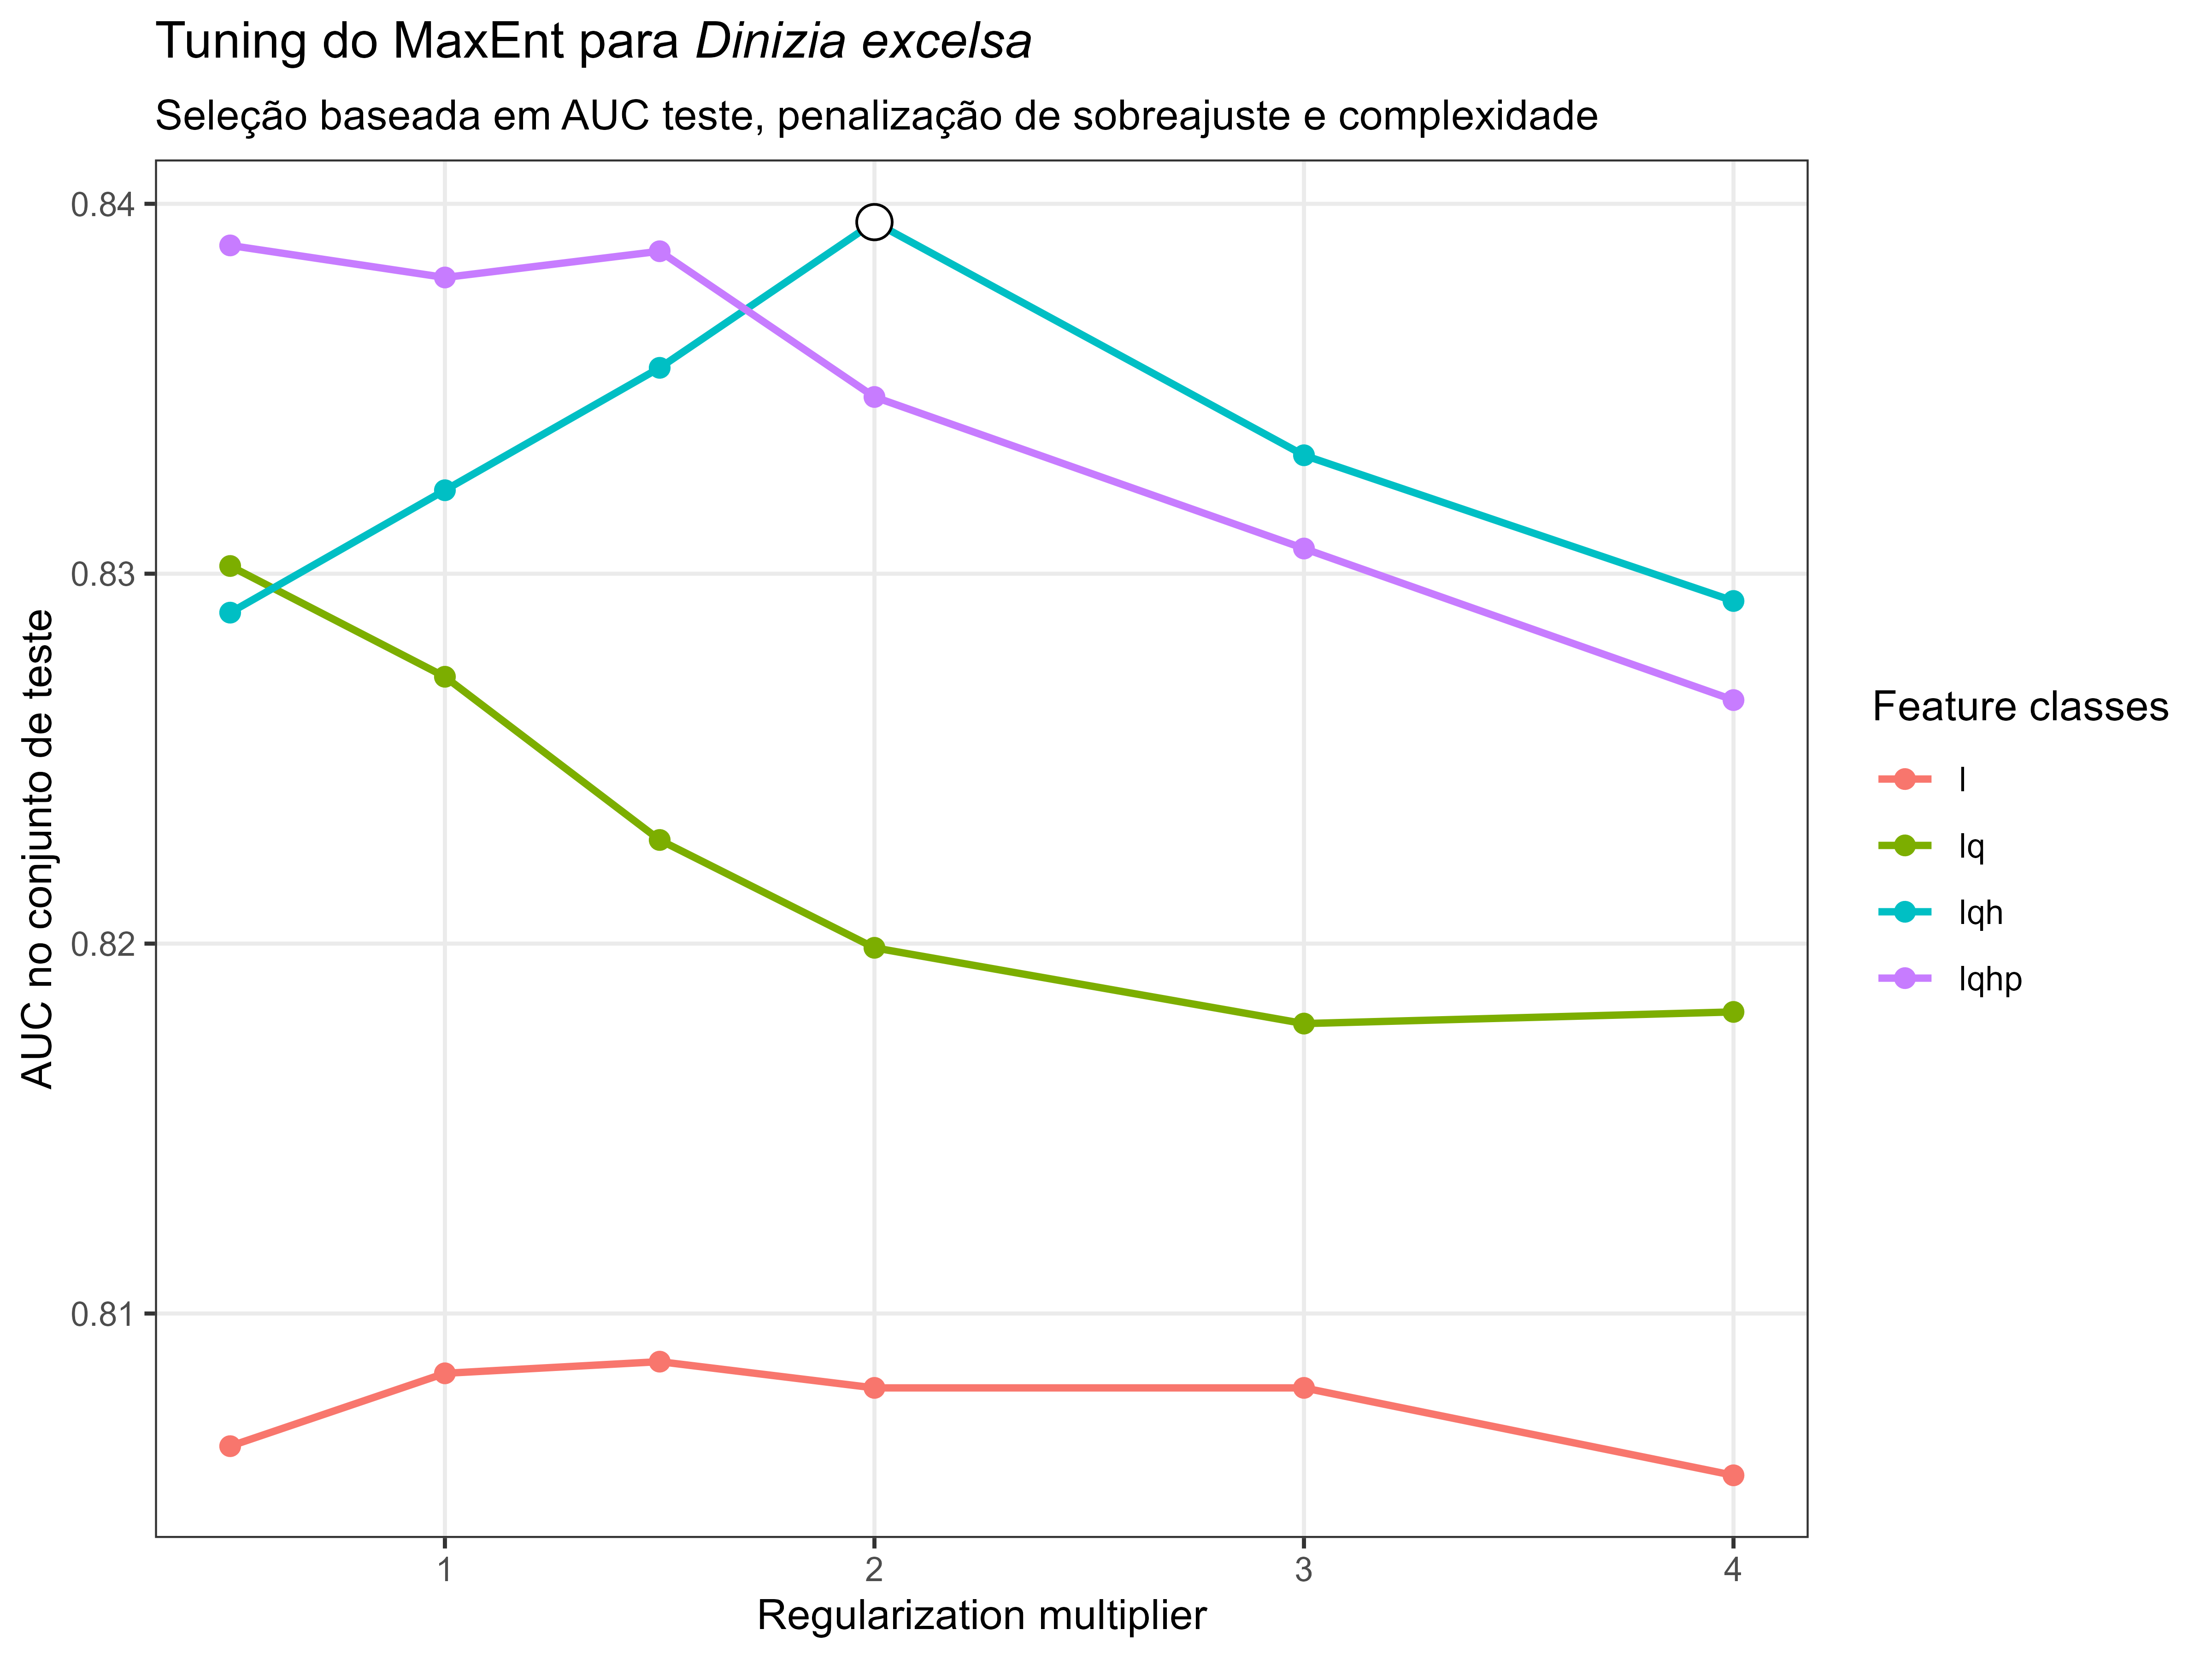
\includegraphics[width=0.88\textwidth]{figuras/unidade10/unidade10_tuning_maxent.png}
  \caption{Maxent tuning results for \textit{Dinizia excelsa} across feature-class combinations and regularization multipliers.}
  \label{fig:unidade10_tuning_maxent}
\end{figure}

\section{Fitting the Final Maxent Model}

The best supported hyperparameter combination is used to fit the final model.

\rscriptfile{scripts/unidade10/04_ajustar_maxent_final.R}

\begin{figure}[H]
  \centering
  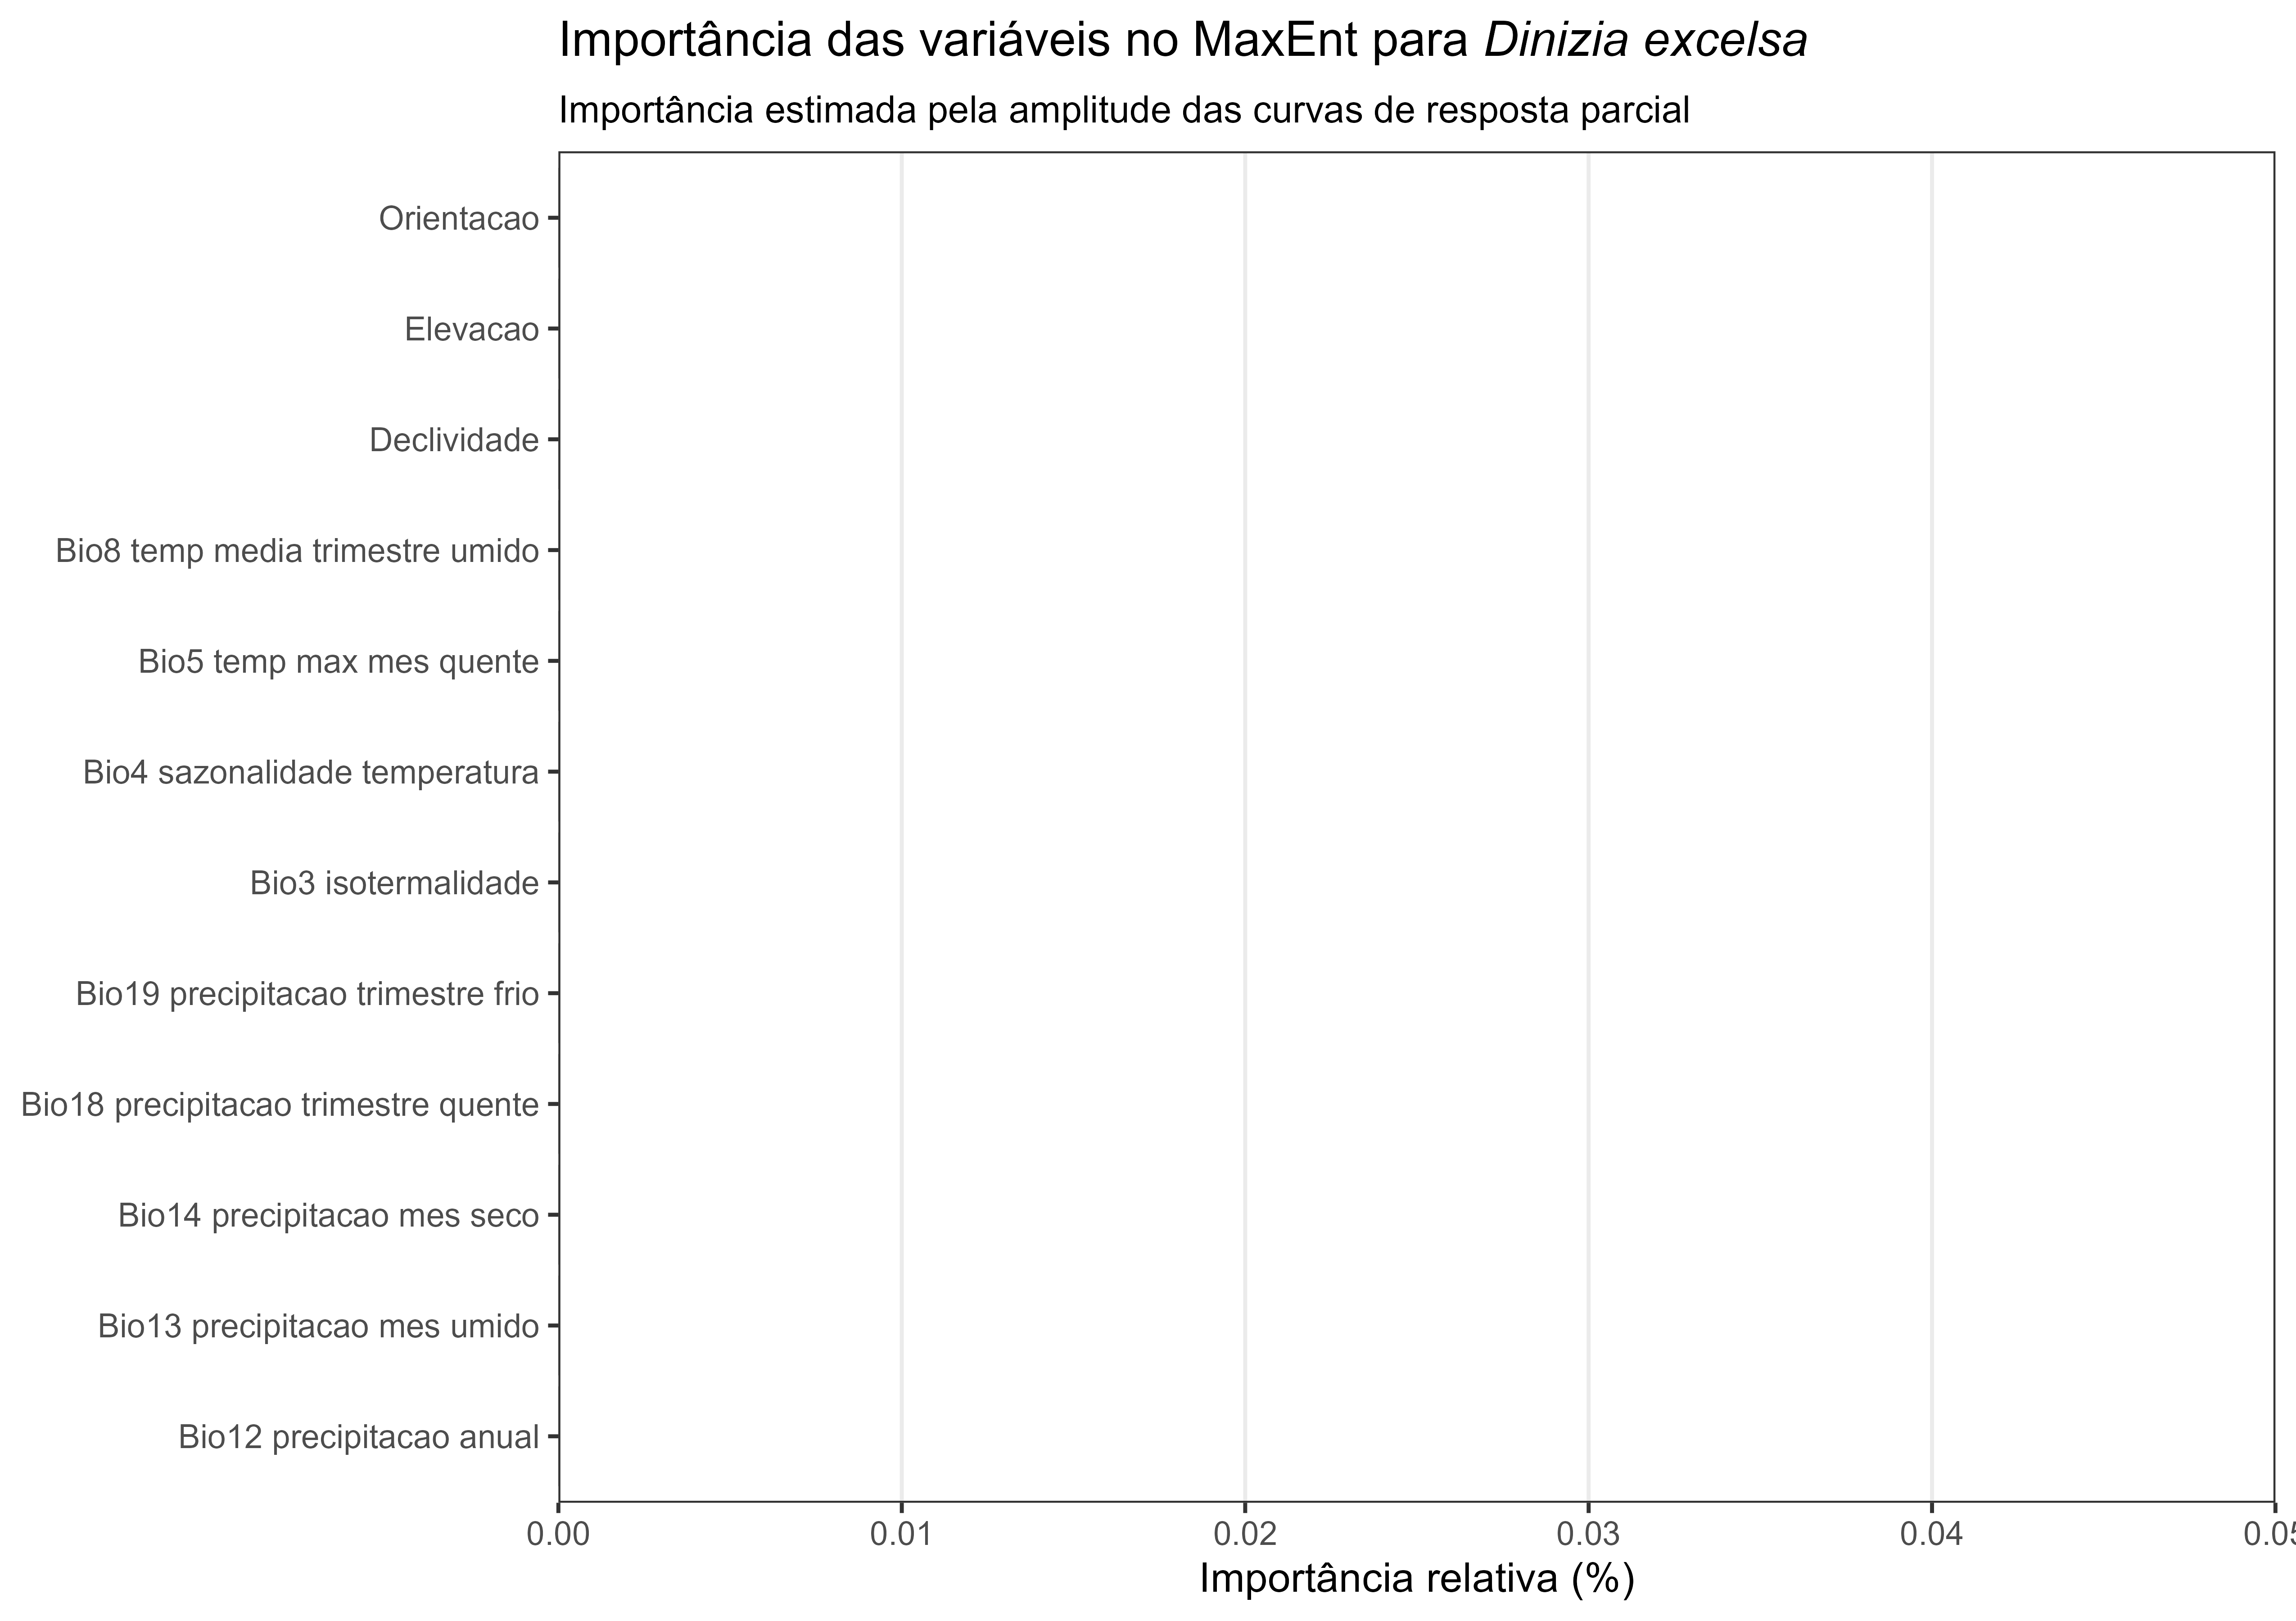
\includegraphics[width=0.86\textwidth]{figuras/unidade10/unidade10_importancia_variaveis_maxent.png}
  \caption{Relative environmental-predictor importance in the final Maxent model for \textit{Dinizia excelsa}.}
  \label{fig:unidade10_importancia_maxent}
\end{figure}

\section{Model Evaluation}

The final model is evaluated on independent test data using AUC, TSS,
sensitivity, specificity, and a confusion matrix.

\rscriptfile{scripts/unidade10/05_avaliar_maxent_dinizia.R}

\begin{figure}[H]
  \centering
  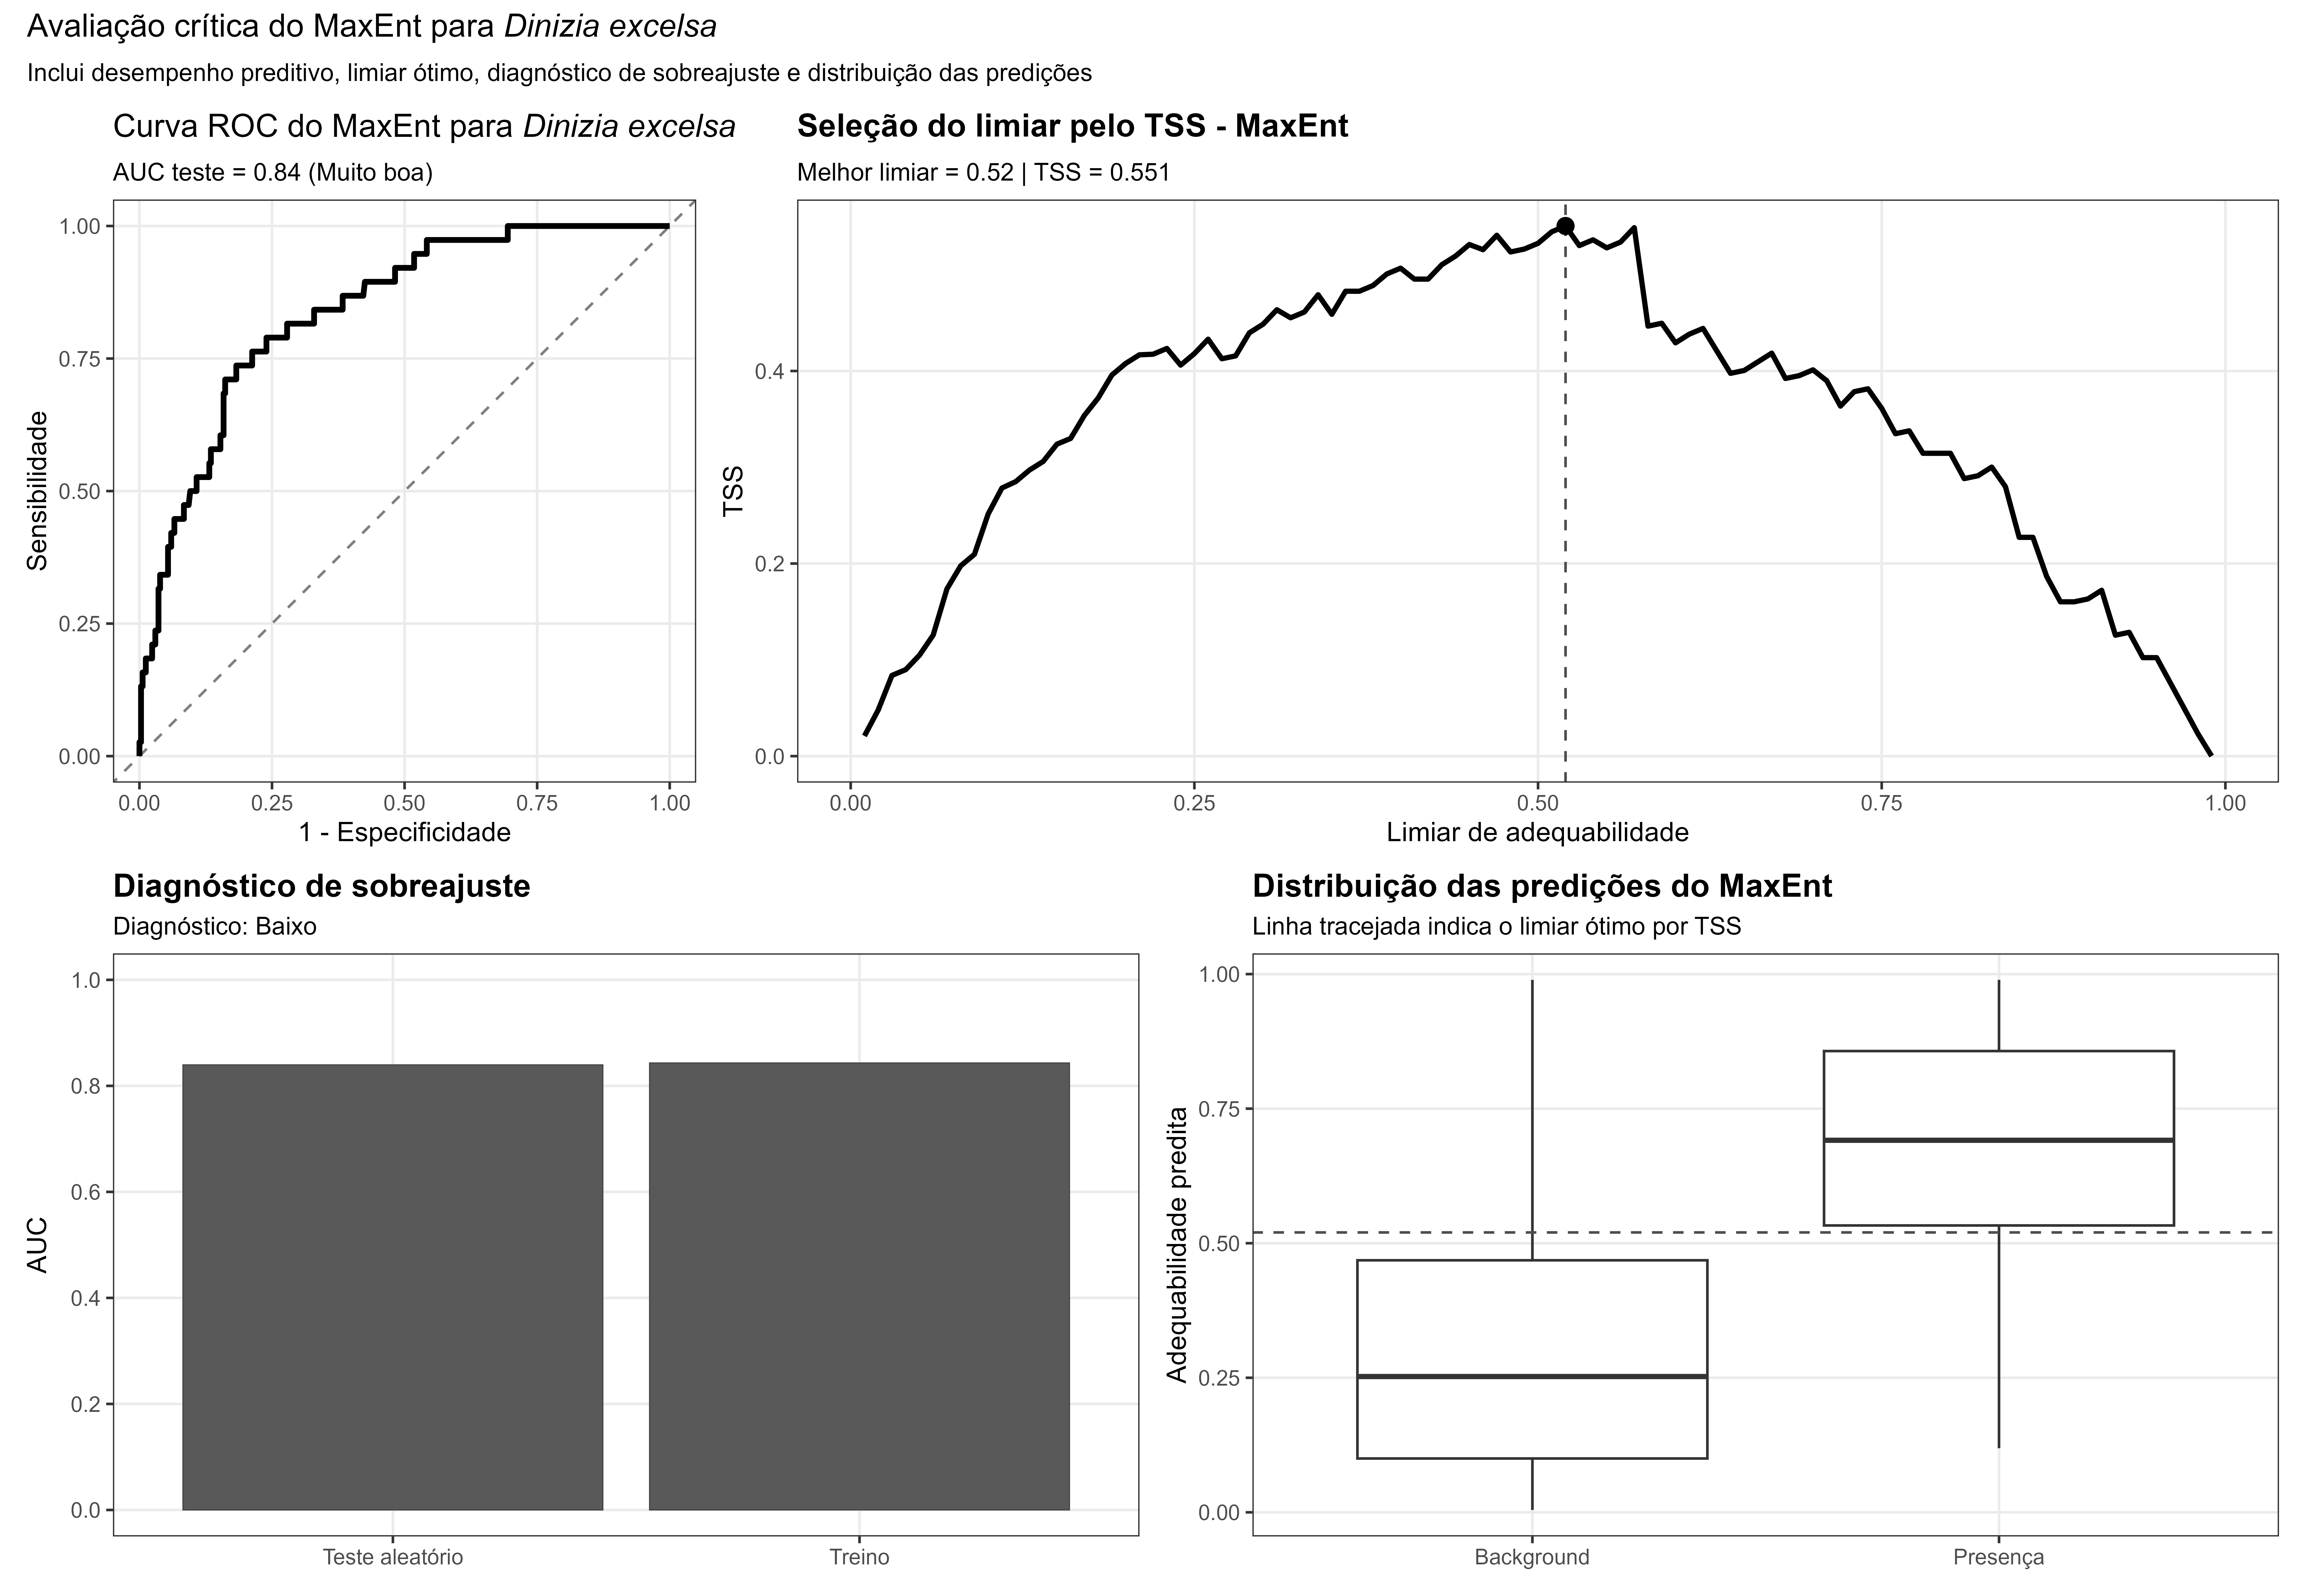
\includegraphics[width=0.78\textwidth]{figuras/unidade10/unidade10_avaliacao_maxent_patchwork.png}
  \caption{ROC curve for Maxent evaluated on the \textit{Dinizia excelsa} test set.}
  \label{fig:unidade10_roc_maxent}
\end{figure}

\section{Current Suitability Map}

The final model is projected across $M$ to produce a continuous current
suitability map.

\rscriptfile{scripts/unidade10/06_predicao_espacial_maxent.R}

\begin{figure}[H]
  \centering
  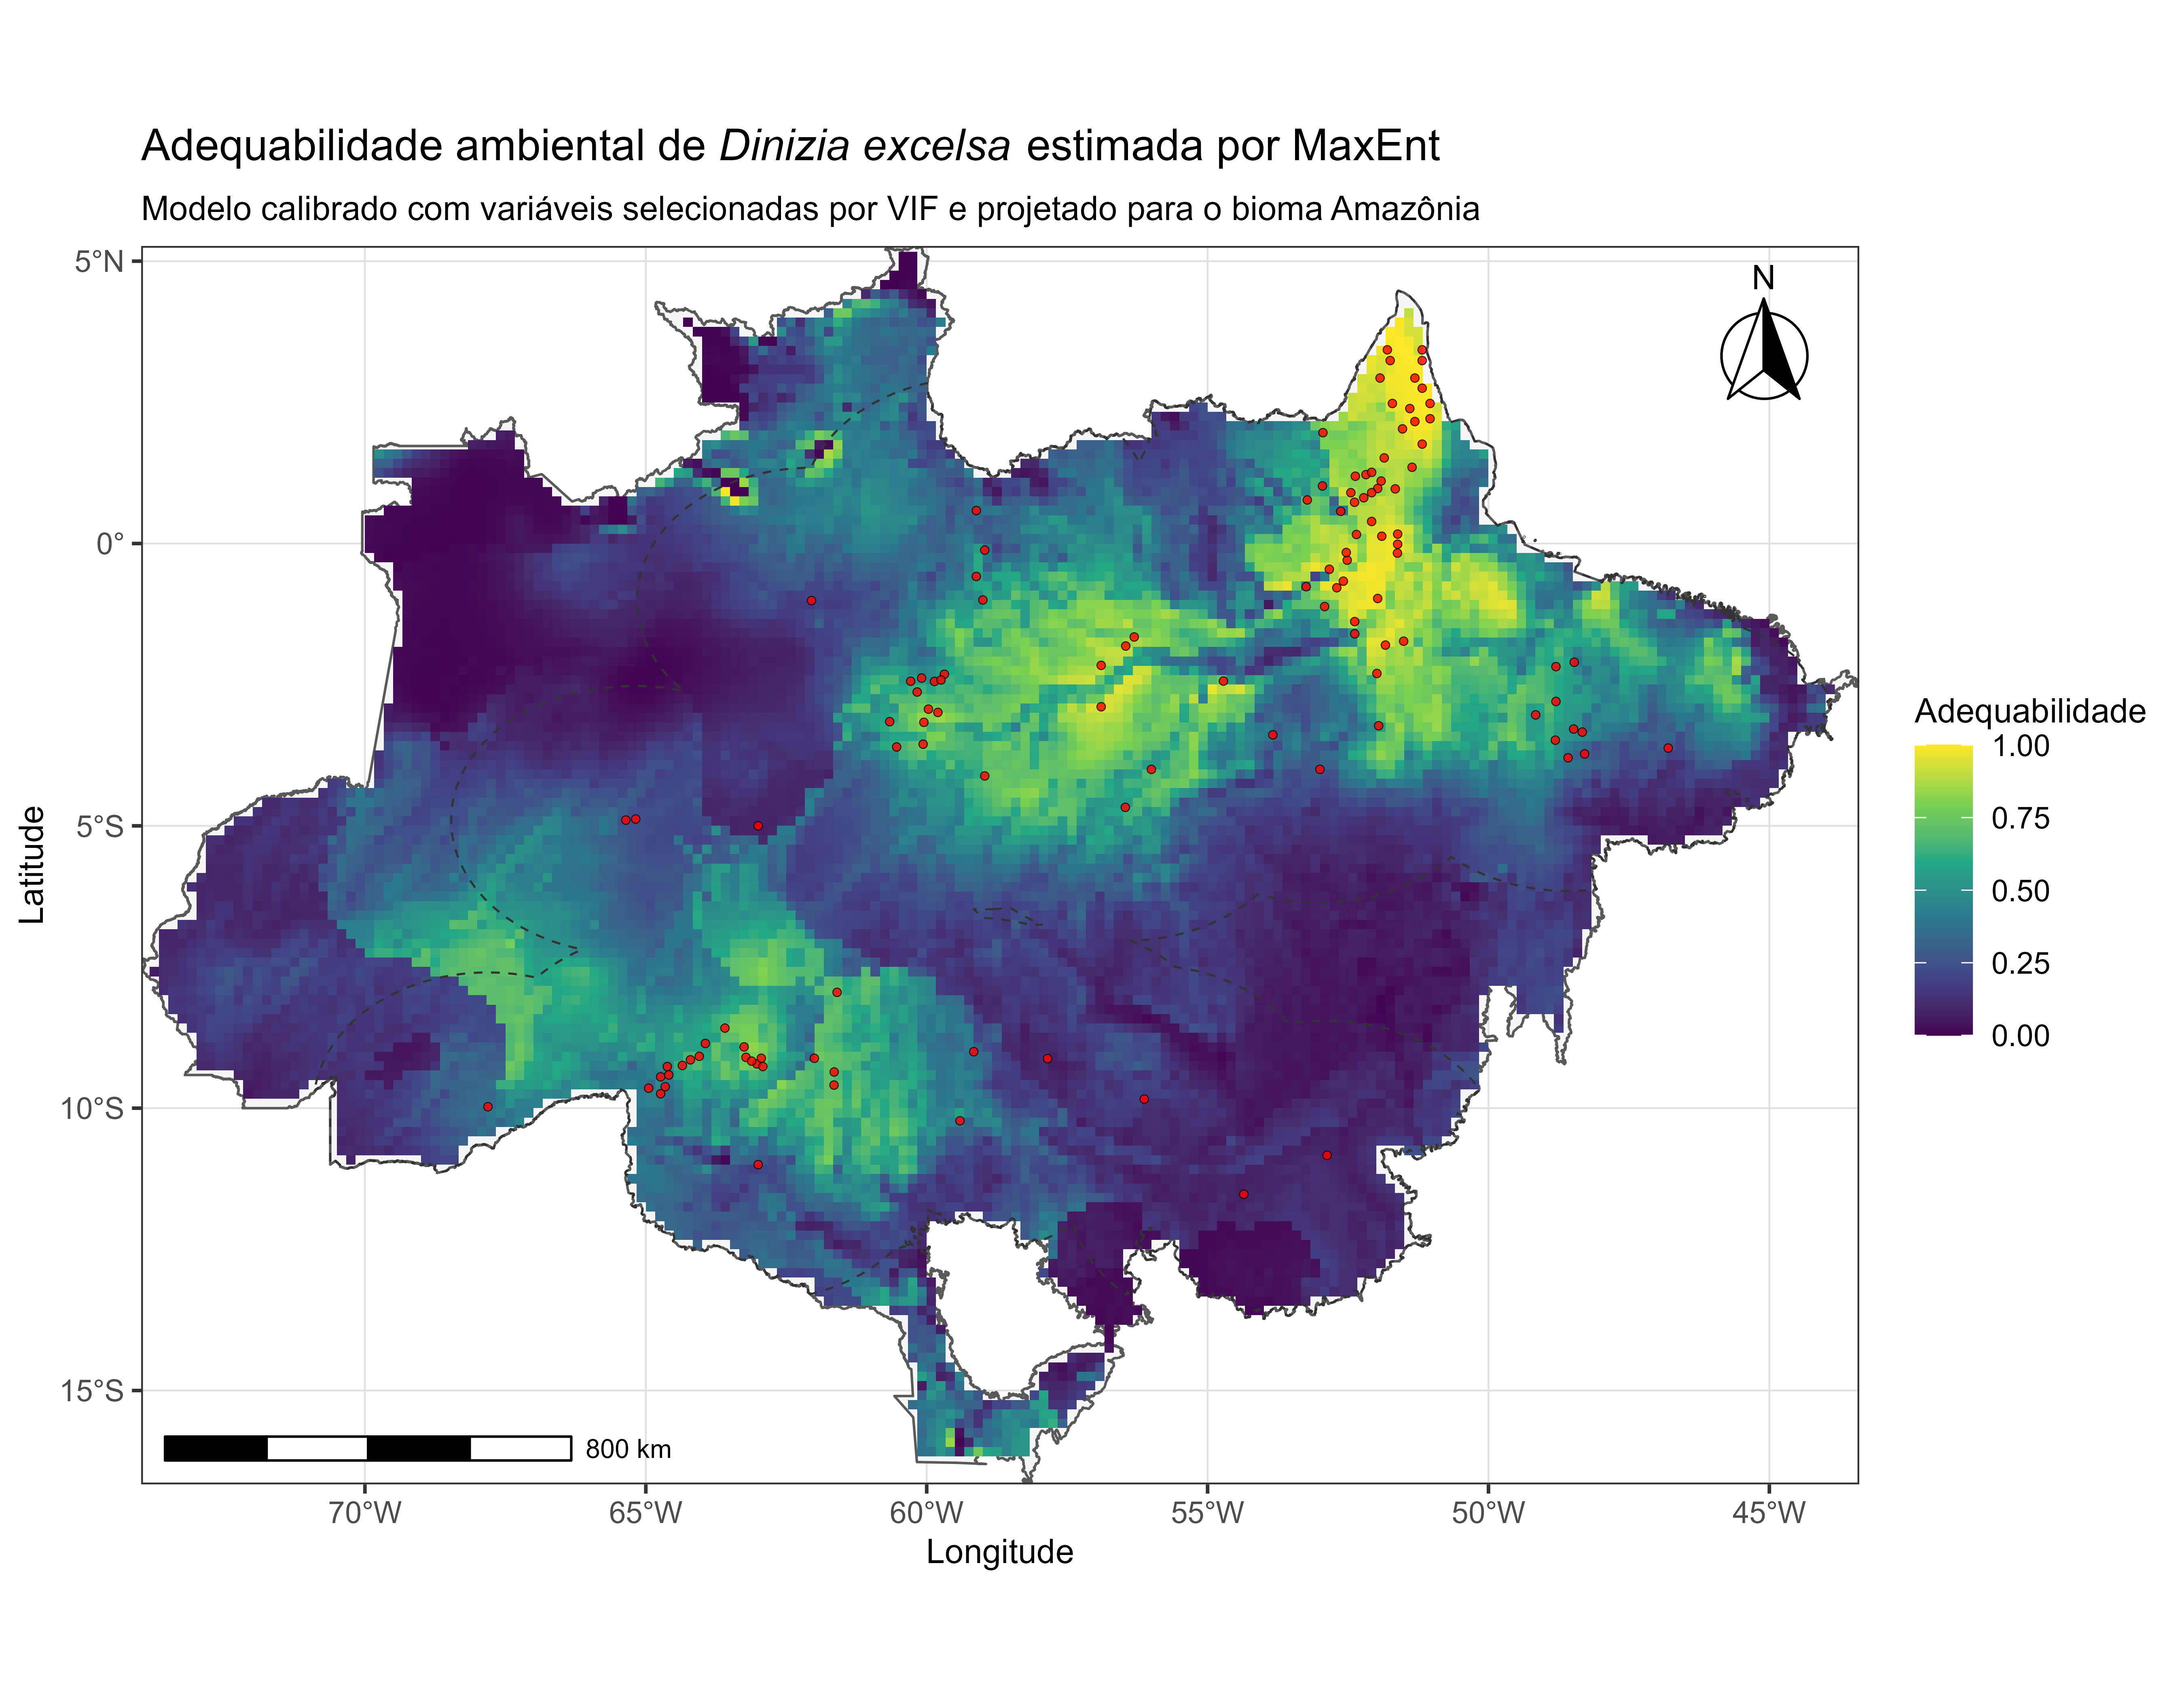
\includegraphics[width=0.88\textwidth]{figuras/unidade10/unidade10_adequabilidade_maxent.png}
  \caption{Current suitability for \textit{Dinizia excelsa} estimated by Maxent within $M$.}
  \label{fig:unidade10_adequabilidade_maxent}
\end{figure}

\section{Partial Response Curves}
\rscriptfile{scripts/unidade10/07_curvas_resposta_maxent.R}

\begin{figure}[H]
  \centering
  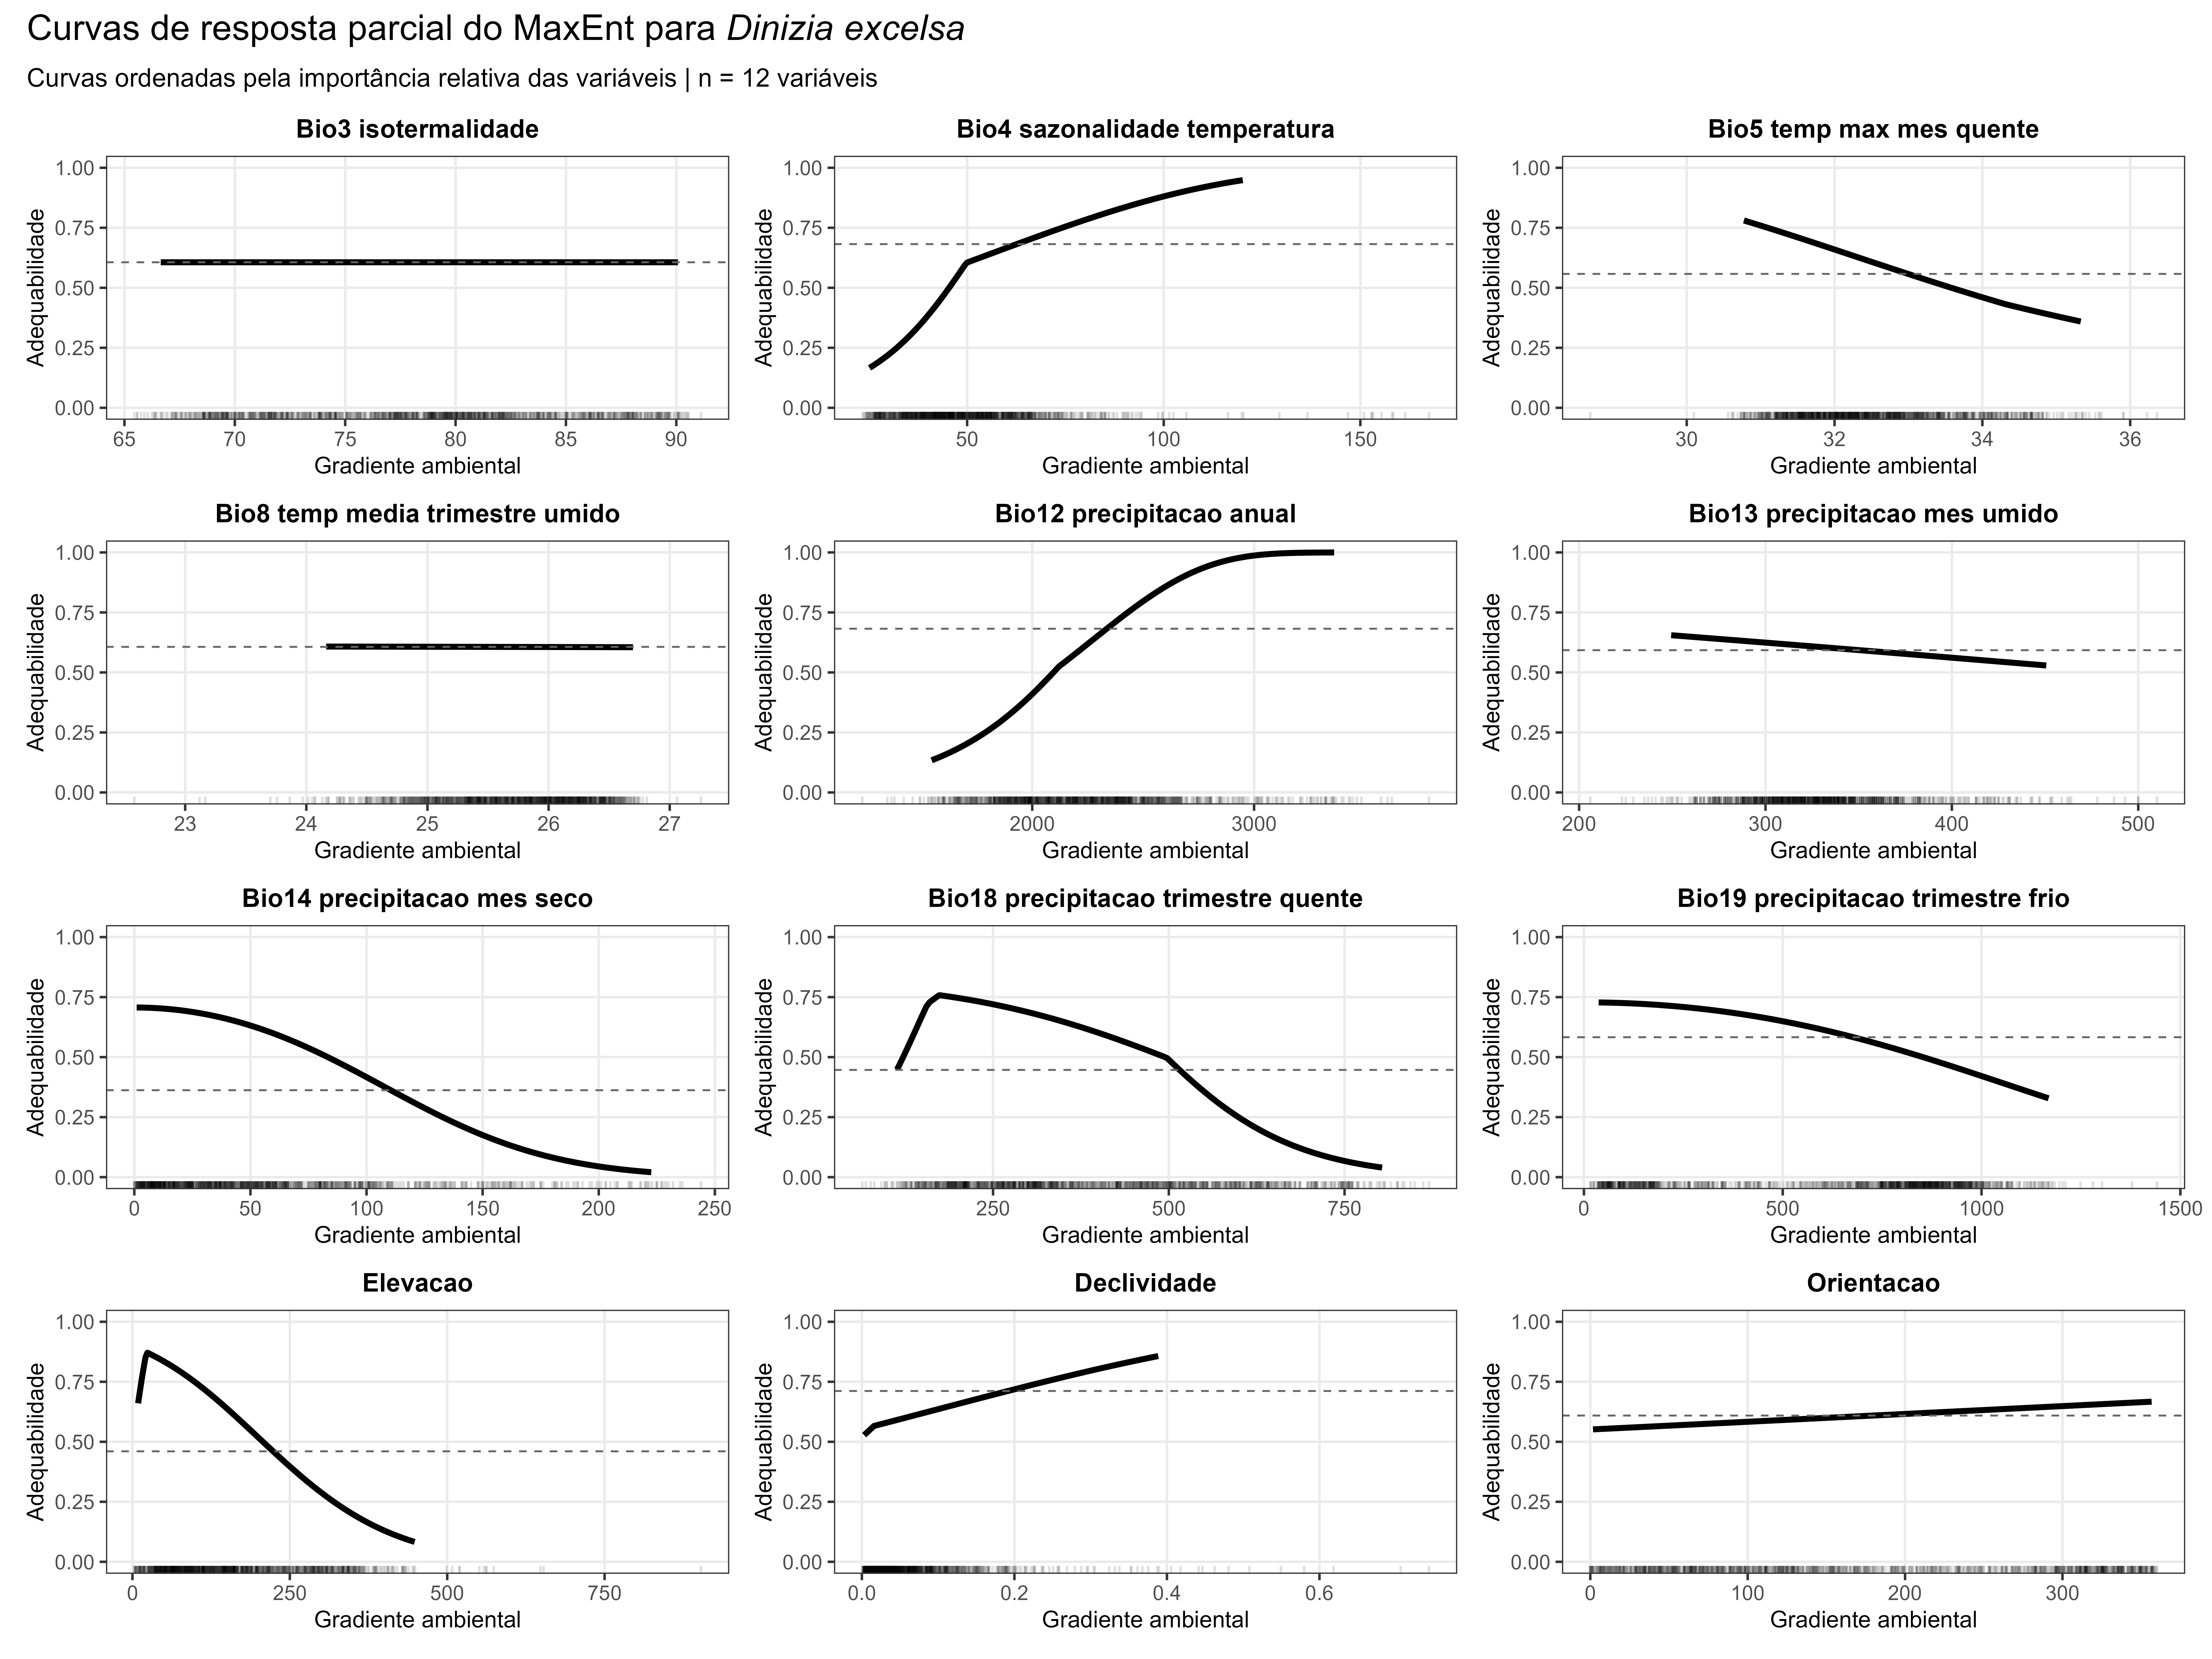
\includegraphics[width=0.96\textwidth]{figuras/unidade10/unidade10_curvas_resposta_maxent.png}
  \caption{Maxent partial response curves for the selected environmental predictors.}
  \label{fig:unidade10_curvas_resposta_maxent}
\end{figure}

\section{Comparison with Previous Models}
\rscriptfile{scripts/unidade10/08_comparar_modelos_maxent.R}

\begin{figure}[H]
  \centering
  \includegraphics[width=0.98\textwidth]{figuras/unidade10/unidade10_comparacao_modelos_maxent.png}
  \caption{Comparison of suitability maps estimated by GLM, GAM, Random Forest, BRT, and Maxent.}
  \label{fig:unidade10_comparacao_modelos}
\end{figure}

\section{Complete Pipeline}
\rscriptfile{scripts/unidade10/09_pipeline_maxent.R}

\section{Chapter Summary}

Maxent is robust and well suited to presence--background data, but responsible
application requires defensible background, feature classes, regularization,
tuning, and validation. Excessive complexity may produce detailed maps that
transfer poorly to new climates or regions.

\begin{figure}[H]
  \centering
  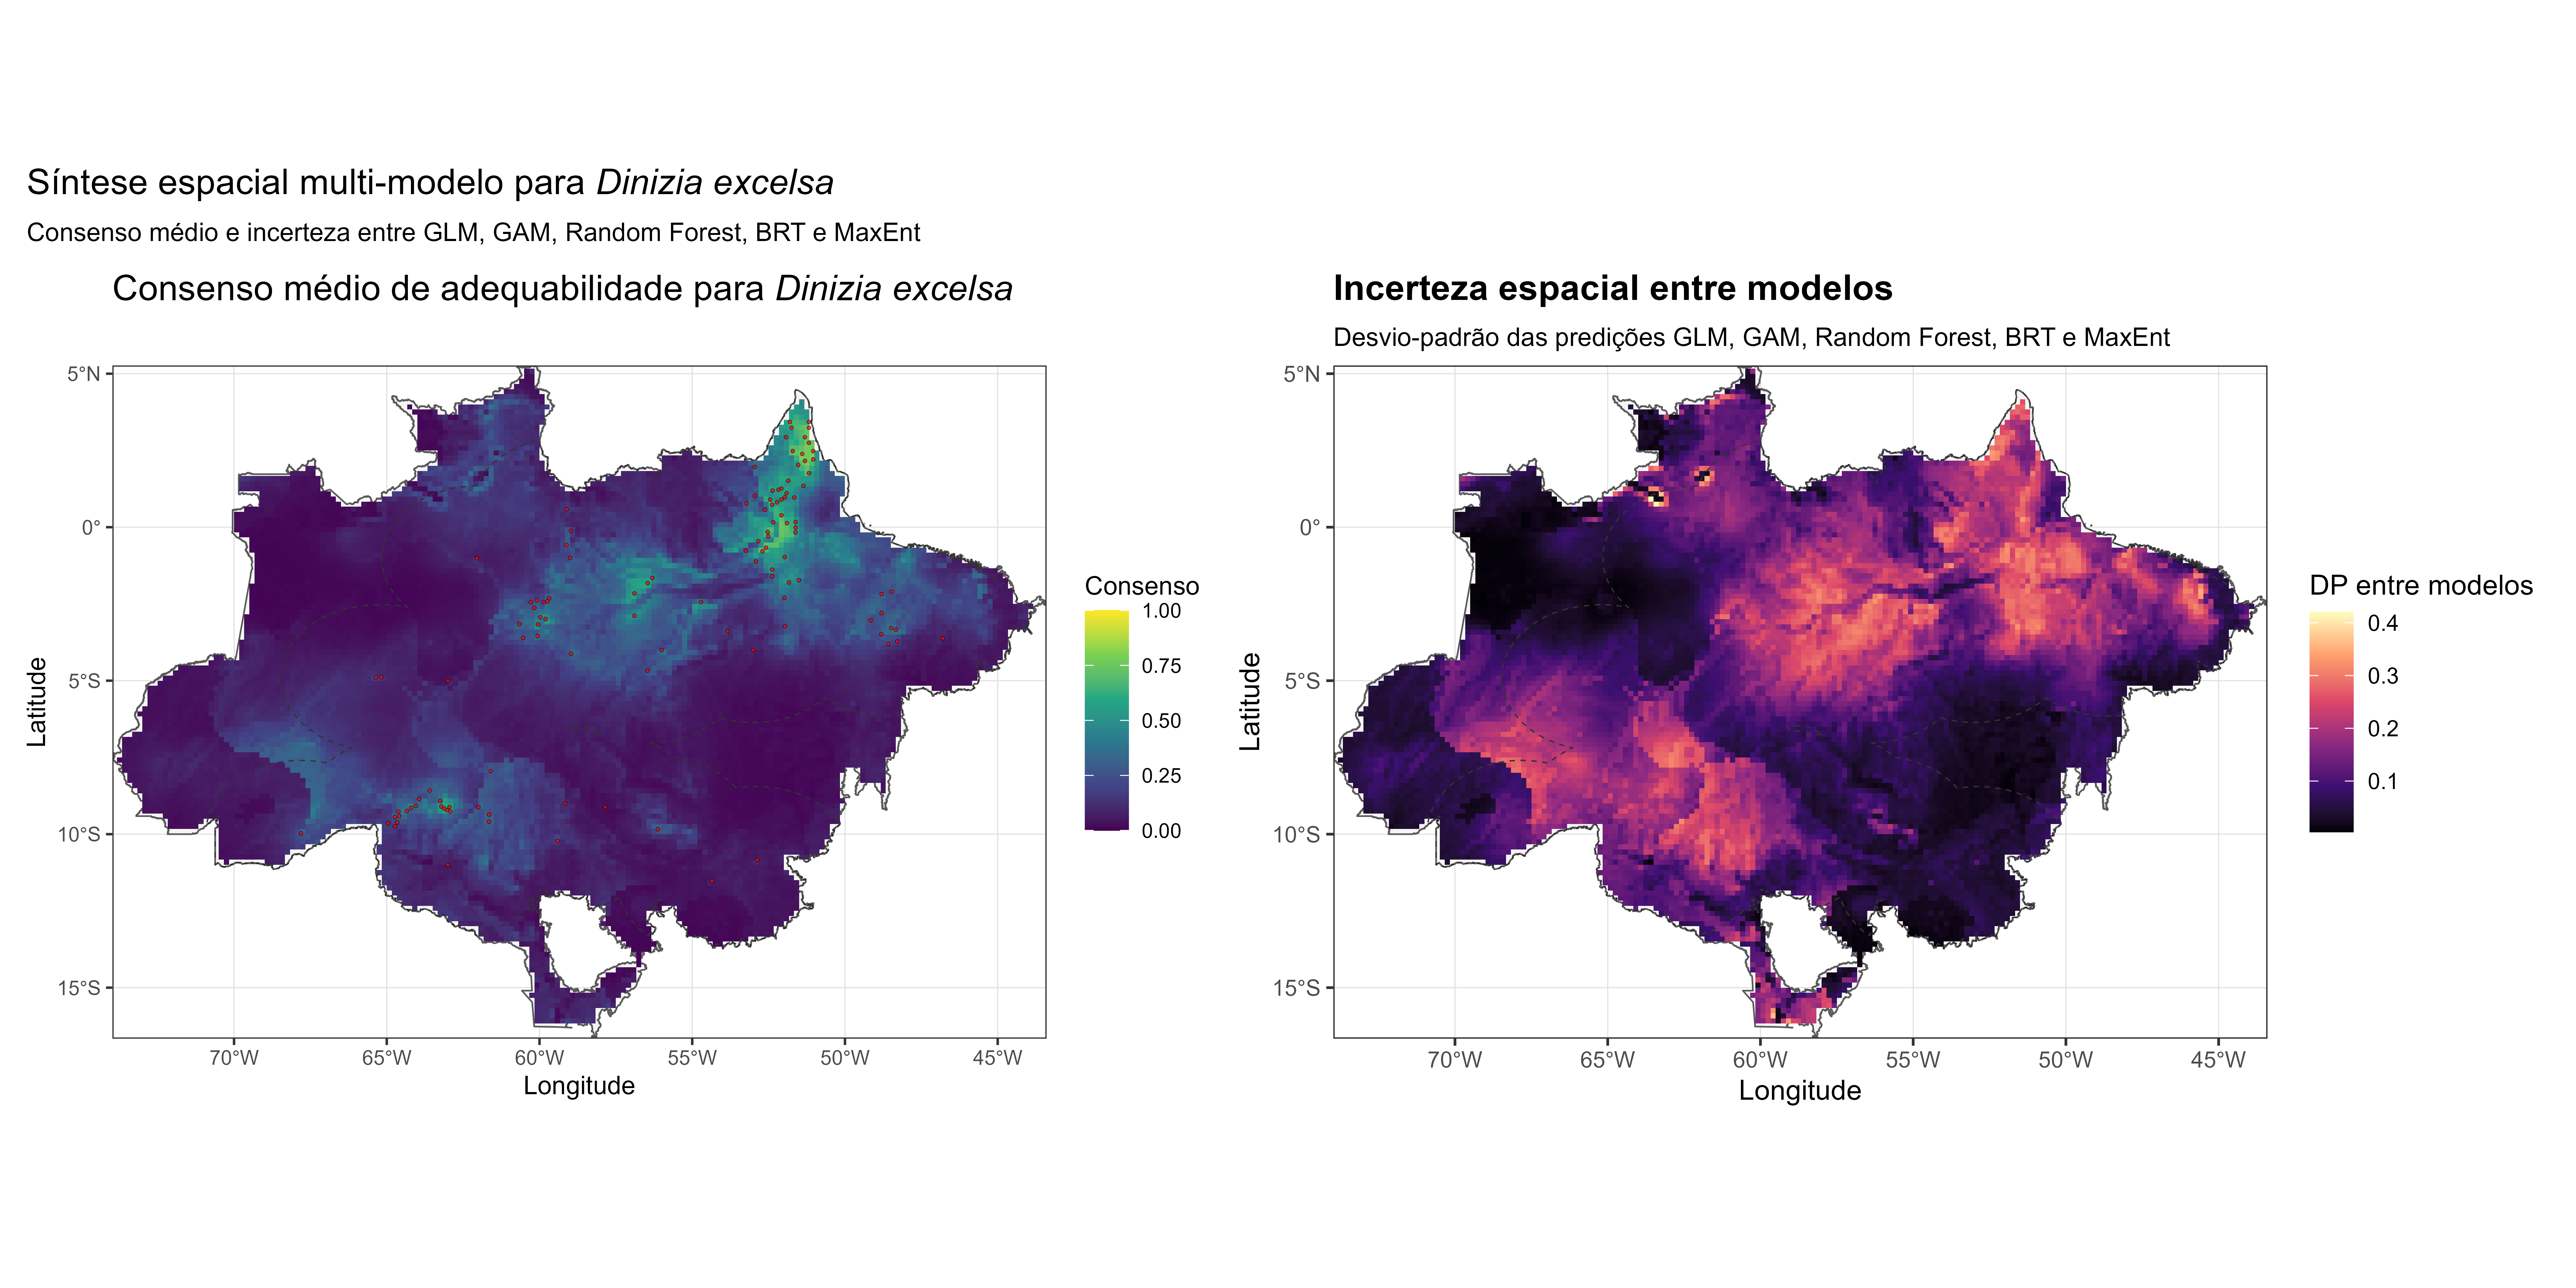
\includegraphics[width=\textwidth]{figuras/unidade10/unidade10_sintese_consenso_incerteza_glm_gam_rf_brt_maxent.png}
  \caption{Multimodel synthesis for \textit{Dinizia excelsa} across Amazonia. The left panel is mean suitability from GLM, GAM, Random Forest, BRT, and Maxent. The right panel is their standard deviation. High consensus indicates agreement on suitability; high standard deviation identifies stronger algorithmic disagreement.}
  \label{fig:unidade10_consenso_incerteza}
\end{figure}

\begin{conceito}[title={\faBook\quad Key message}]
Maxent should not be treated as a black box. Its performance depends on $M$,
background, predictor selection, regularization, and independent evaluation.
\end{conceito}

\subsection*{Comparative Synthesis of the Algorithms}

Table~\ref{tab:comparacao_algoritmos_sdm} summarizes conceptual differences,
operational strengths, methodological limitations, and interpretability.

\begin{table}[H]
\centering
\caption{Comparison of major algorithms used in species distribution modeling.}
\label{tab:comparacao_algoritmos_sdm}
\scriptsize
\setlength{\tabcolsep}{2.5pt}
\begin{tabular}{p{0.10\textwidth}p{0.14\textwidth}p{0.12\textwidth}p{0.19\textwidth}p{0.19\textwidth}p{0.14\textwidth}}
\toprule
\textbf{Method} & \textbf{Data type} & \textbf{Response} & \textbf{Strengths} & \textbf{Limitations} & \textbf{Interpretability} \\
\midrule
GLM & Presence--absence & Linear & Simple, robust, widely used & Limited flexibility for complex responses & Excellent \\
GAM & Presence--absence & Nonlinear & Flexible and interpretable & More complex than GLM & Very high \\
Random Forest & Presence--absence & Nonlinear & Strong predictive performance & Lower ecological interpretability & Moderate \\
BRT & Presence--absence & Nonlinear & Captures interactions and nonlinearities & Delicate hyperparameter tuning & Moderate \\
Maxent & Presence--background & Nonlinear & Well suited to presence-only records & Sensitive to background and sampling bias & Good \\
Ensemble & Multiple & Integrated & Represents algorithmic consensus and disagreement & More complex to interpret & Variable \\
\bottomrule
\end{tabular}
\end{table}

\subsection*{Practical Guide to Algorithm Selection}

\begin{table}[H]
\centering
\caption{Practical guide to selecting algorithms for different SDM applications.}
\label{tab:guia_escolha_algoritmos}
\small
\begin{tabular}{p{0.48\textwidth}p{0.36\textwidth}}
\toprule
\textbf{Situation} & \textbf{Candidate method} \\
\midrule
Few occurrence records & Maxent \\
Ecological interpretation of environmental effects & GLM or GAM \\
Prediction emphasizing statistical performance & Random Forest or BRT \\
Biodiversity-conservation modeling & Ensemble \\
Climate-change projections & Ensemble \\
Initial exploratory analysis & GLM \\
Ecological response curves & GAM \\
Relative predictor importance & Random Forest or BRT \\
Presence-only records & Maxent \\
Representation of algorithmic consensus and disagreement & Ensemble \\
\bottomrule
\end{tabular}
\end{table}

\begin{center}
\fbox{\begin{minipage}{0.90\textwidth}
\textbf{Methodological synthesis.} No algorithm is universally superior. Model
performance depends on data quality, $M$, predictor selection, validation, and
the ecological question. Ensembles are often useful in conservation and climate
change applications because they reduce dependence on a single algorithm and
explicitly represent between-algorithm variation; they do not automatically
eliminate bias shared by all component models.
\end{minipage}}
\end{center}

\section{Review Exercises}
\begin{enumerate}
  \item Explain the maximum entropy principle.
  \item Distinguish presence, absence, and background data.
  \item What are feature classes in Maxent?
  \item What is the role of regularization?
  \item Why can highly complex Maxent models be problematic?
  \item Why is tuning required?
  \item Compare Maxent with GLM, GAM, Random Forest, and BRT.
\end{enumerate}

\chapter[Ensemble Modeling]{Ensemble Modeling}

\begin{objetivos}
By the end of this chapter, readers should understand ensemble SDM; integrate
GLM, GAM, Random Forest, BRT, and Maxent predictions; compare unweighted means,
performance-weighted means, and binary consensus; map ensemble suitability and
between-model agreement for \textit{Dinizia excelsa}; and prepare outputs for
future projections, uncertainty assessment, and conservation applications.
\end{objetivos}

\section{Introduction}

Ensemble modeling combines predictions from different algorithms rather than
depending on a single representation of the occurrence--environment relationship
\parencite{araujo2007ensemble,thuiller2009biomod,guisan2017habitat}. Algorithms
differ in response shape and flexibility: GLM and GAM are comparatively
interpretable, Random Forest and BRT capture complex structure, and Maxent is
designed for presence--background data. An ensemble summarizes this variation.

\begin{conceito}[title={\faBook\quad Ensembles in SDM}]
An ensemble combines multiple model predictions into an integrated suitability
estimate. It does not eliminate uncertainty; it makes agreement and disagreement
among algorithms explicit.
\end{conceito}

\section{Types of Ensemble}
\begin{itemize}
  \item unweighted mean prediction;
  \item mean weighted by predictive performance; and
  \item binary consensus based on presence--absence thresholds.
\end{itemize}
The unweighted mean assigns equal influence. A weighted mean favors models with
stronger evaluation scores. Binary consensus is the proportion of models that
classify a cell as suitable.

\begin{atencao}[title={\faExclamationTriangle\quad An ensemble does not repair a poor model}]
Only models meeting defensible quality criteria should enter the ensemble.
Including severely overfitted, low-quality, or ecologically incoherent models
can degrade the synthesis.
\end{atencao}

\section{Preparing Predictions}
The suitability rasters from Chapters 6--10 must share extent, resolution,
projection, and spatial mask.
\rscriptfile{scripts/unidade11/01_estrutura_pastas.R}
\rscriptfile{scripts/unidade11/02_preparar_predicoes_ensemble.R}

\section{Unweighted Mean Ensemble}
An unweighted mean is transparent and useful when component models have similar
performance.
\rscriptfile{scripts/unidade11/03_ensemble_media_simples.R}
\begin{figure}[H]
\centering
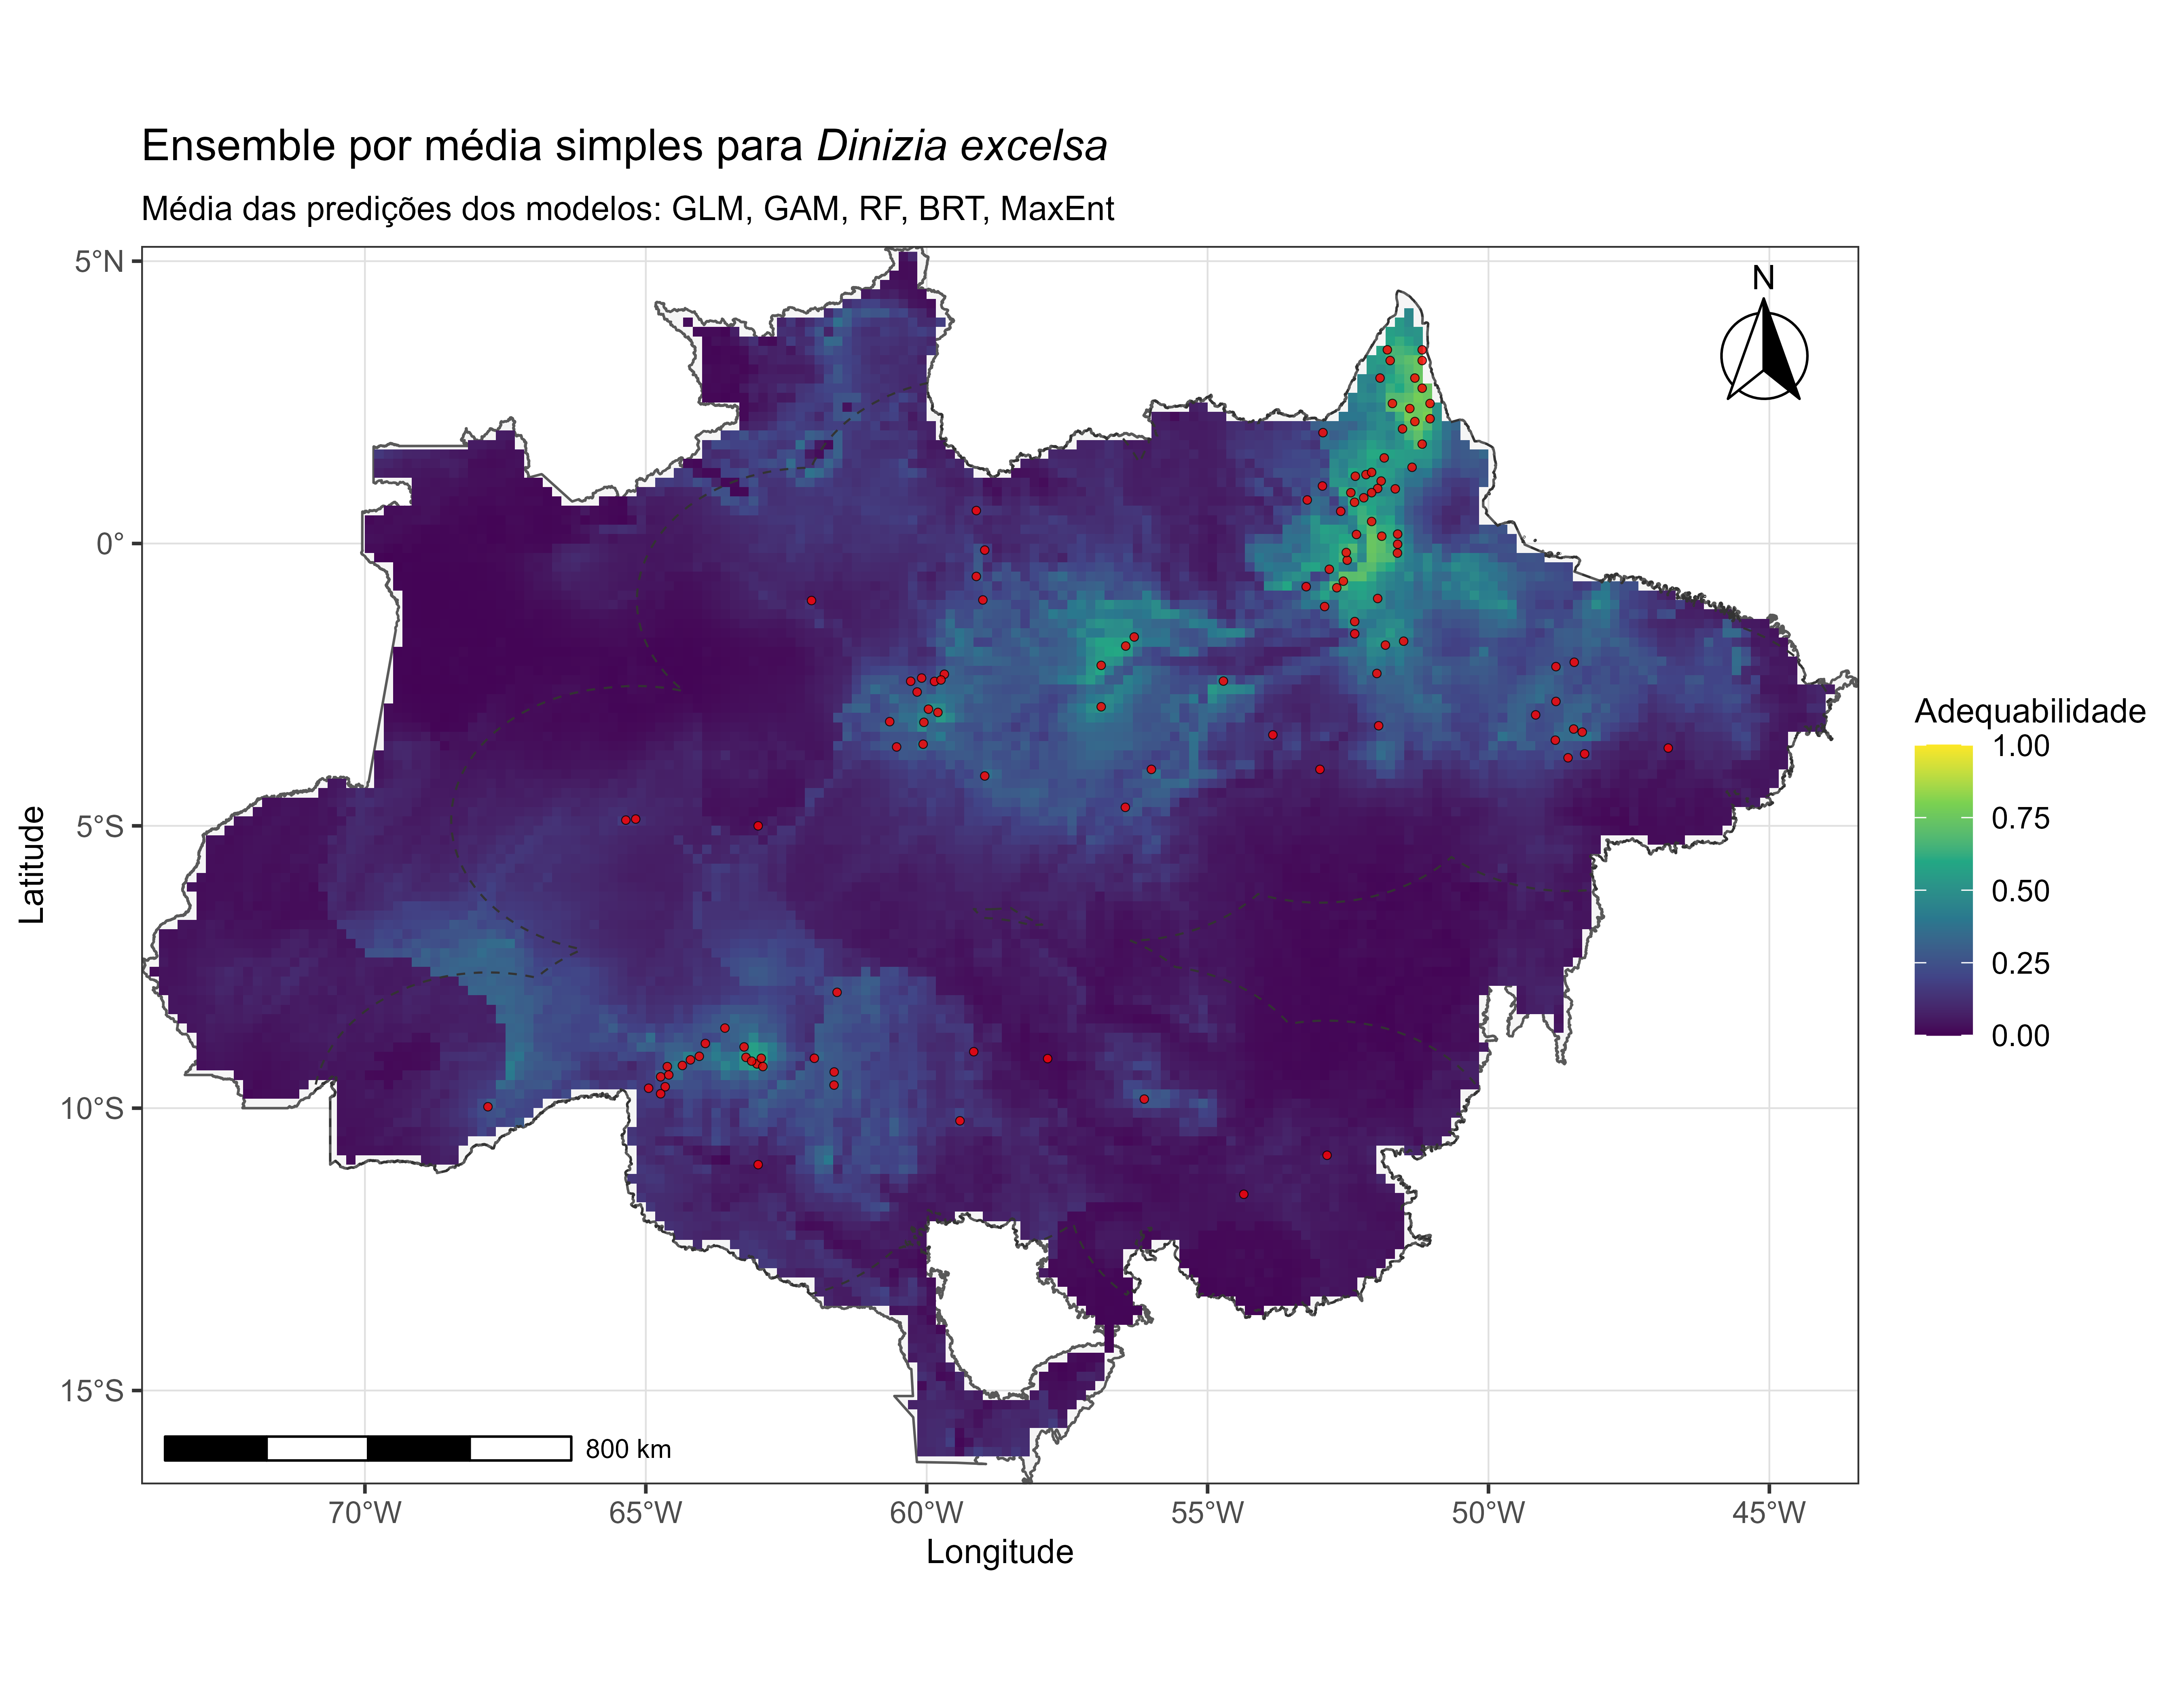
\includegraphics[width=0.88\textwidth]{figuras/unidade11/unidade11_ensemble_media_simples.png}
\caption{Unweighted mean of GLM, GAM, Random Forest, BRT, and Maxent predictions for \textit{Dinizia excelsa}.}
\label{fig:unidade11_ensemble_media}
\end{figure}

\section{Performance-Weighted Ensemble}
A weighted ensemble assigns greater influence to models with stronger
performance. Test AUC is used here, although TSS, Boyce Index, or a composite
criterion could be substituted. Weights inherit the strengths and limitations
of the selected metric and validation design.
\rscriptfile{scripts/unidade11/04_ensemble_ponderado.R}
\begin{figure}[H]
\centering
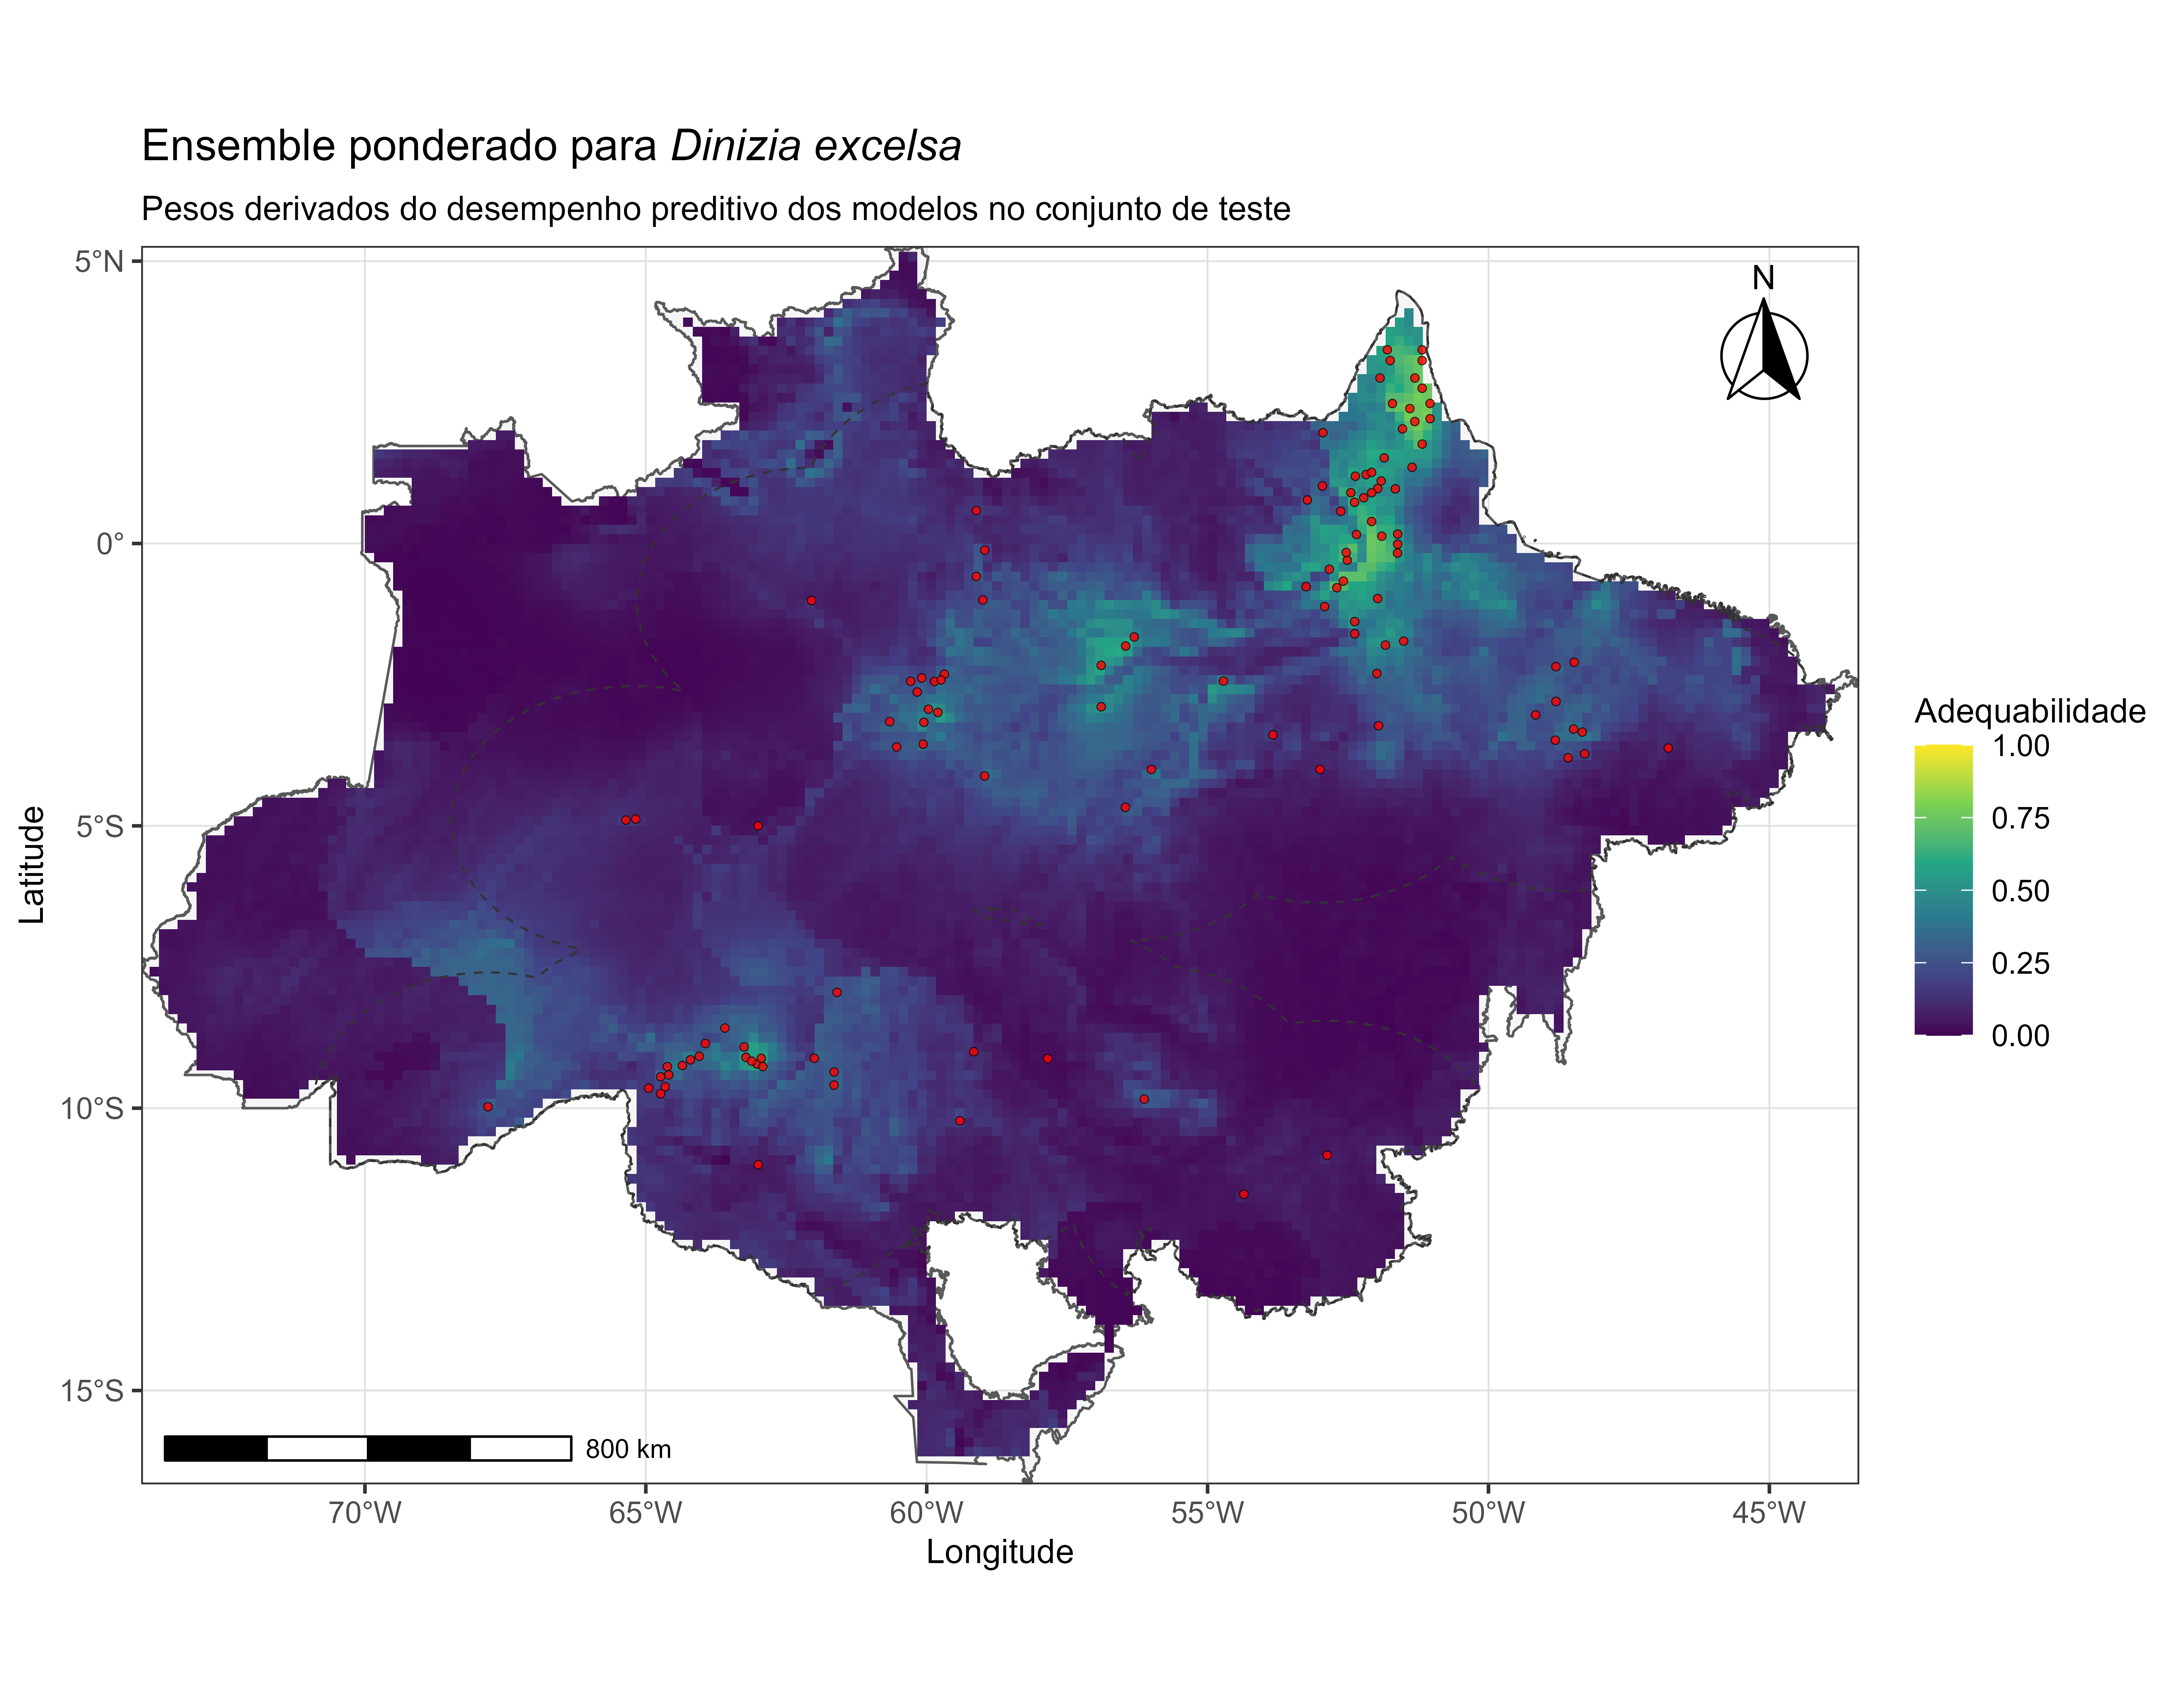
\includegraphics[width=0.88\textwidth]{figuras/unidade11/unidade11_ensemble_ponderado.png}
\caption{Performance-weighted ensemble suitability for \textit{Dinizia excelsa}.}
\label{fig:unidade11_ensemble_ponderado}
\end{figure}

\section{Binary Consensus}
Each continuous map is converted using its TSS threshold. The final value is the
proportion of models classifying a cell as suitable.
\rscriptfile{scripts/unidade11/05_consenso_binario.R}
\begin{figure}[H]
\centering
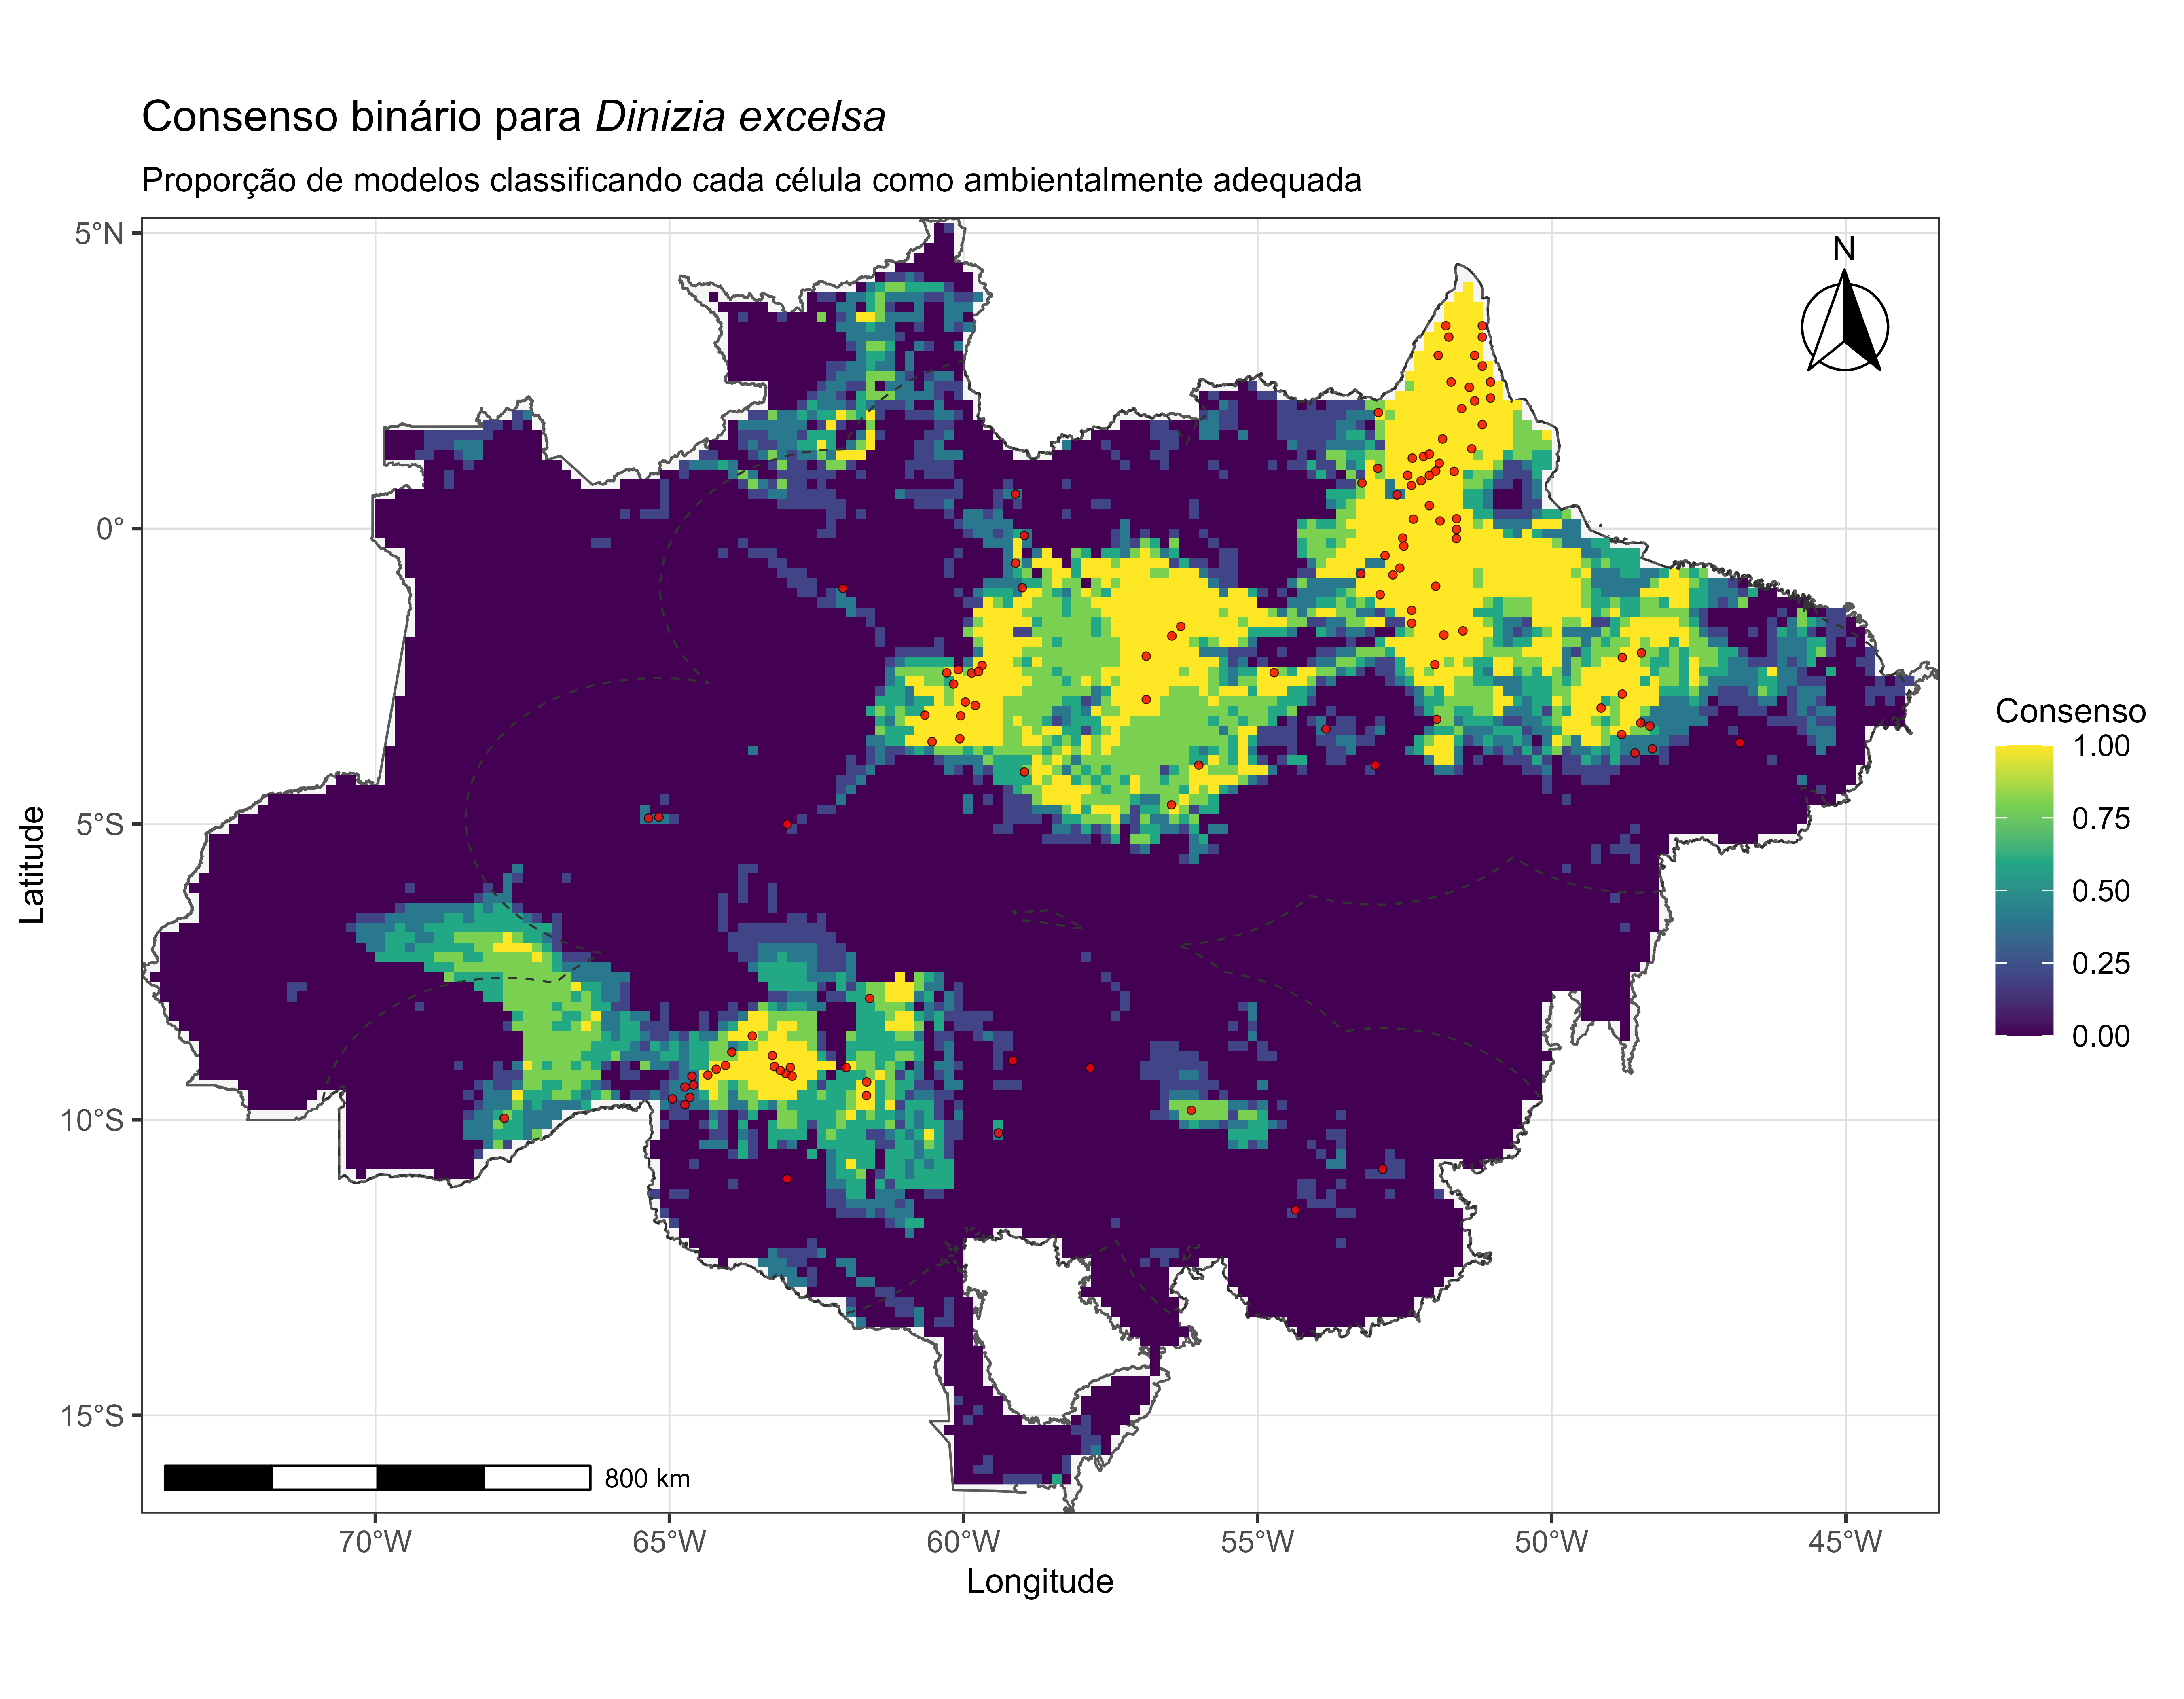
\includegraphics[width=0.88\textwidth]{figuras/unidade11/unidade11_consenso_binario.png}
\caption{Binary model consensus. Values near 1 indicate strong agreement that a cell is environmentally suitable.}
\label{fig:unidade11_consenso_binario}
\end{figure}

\section{Between-Algorithm Disagreement}
Variation among predictions is a descriptive measure of algorithmic disagreement. High mean
suitability with low variation is more robust than high suitability accompanied
by substantial model disagreement.
\rscriptfile{scripts/unidade11/06_incerteza_algoritmica.R}
\begin{figure}[H]
\centering
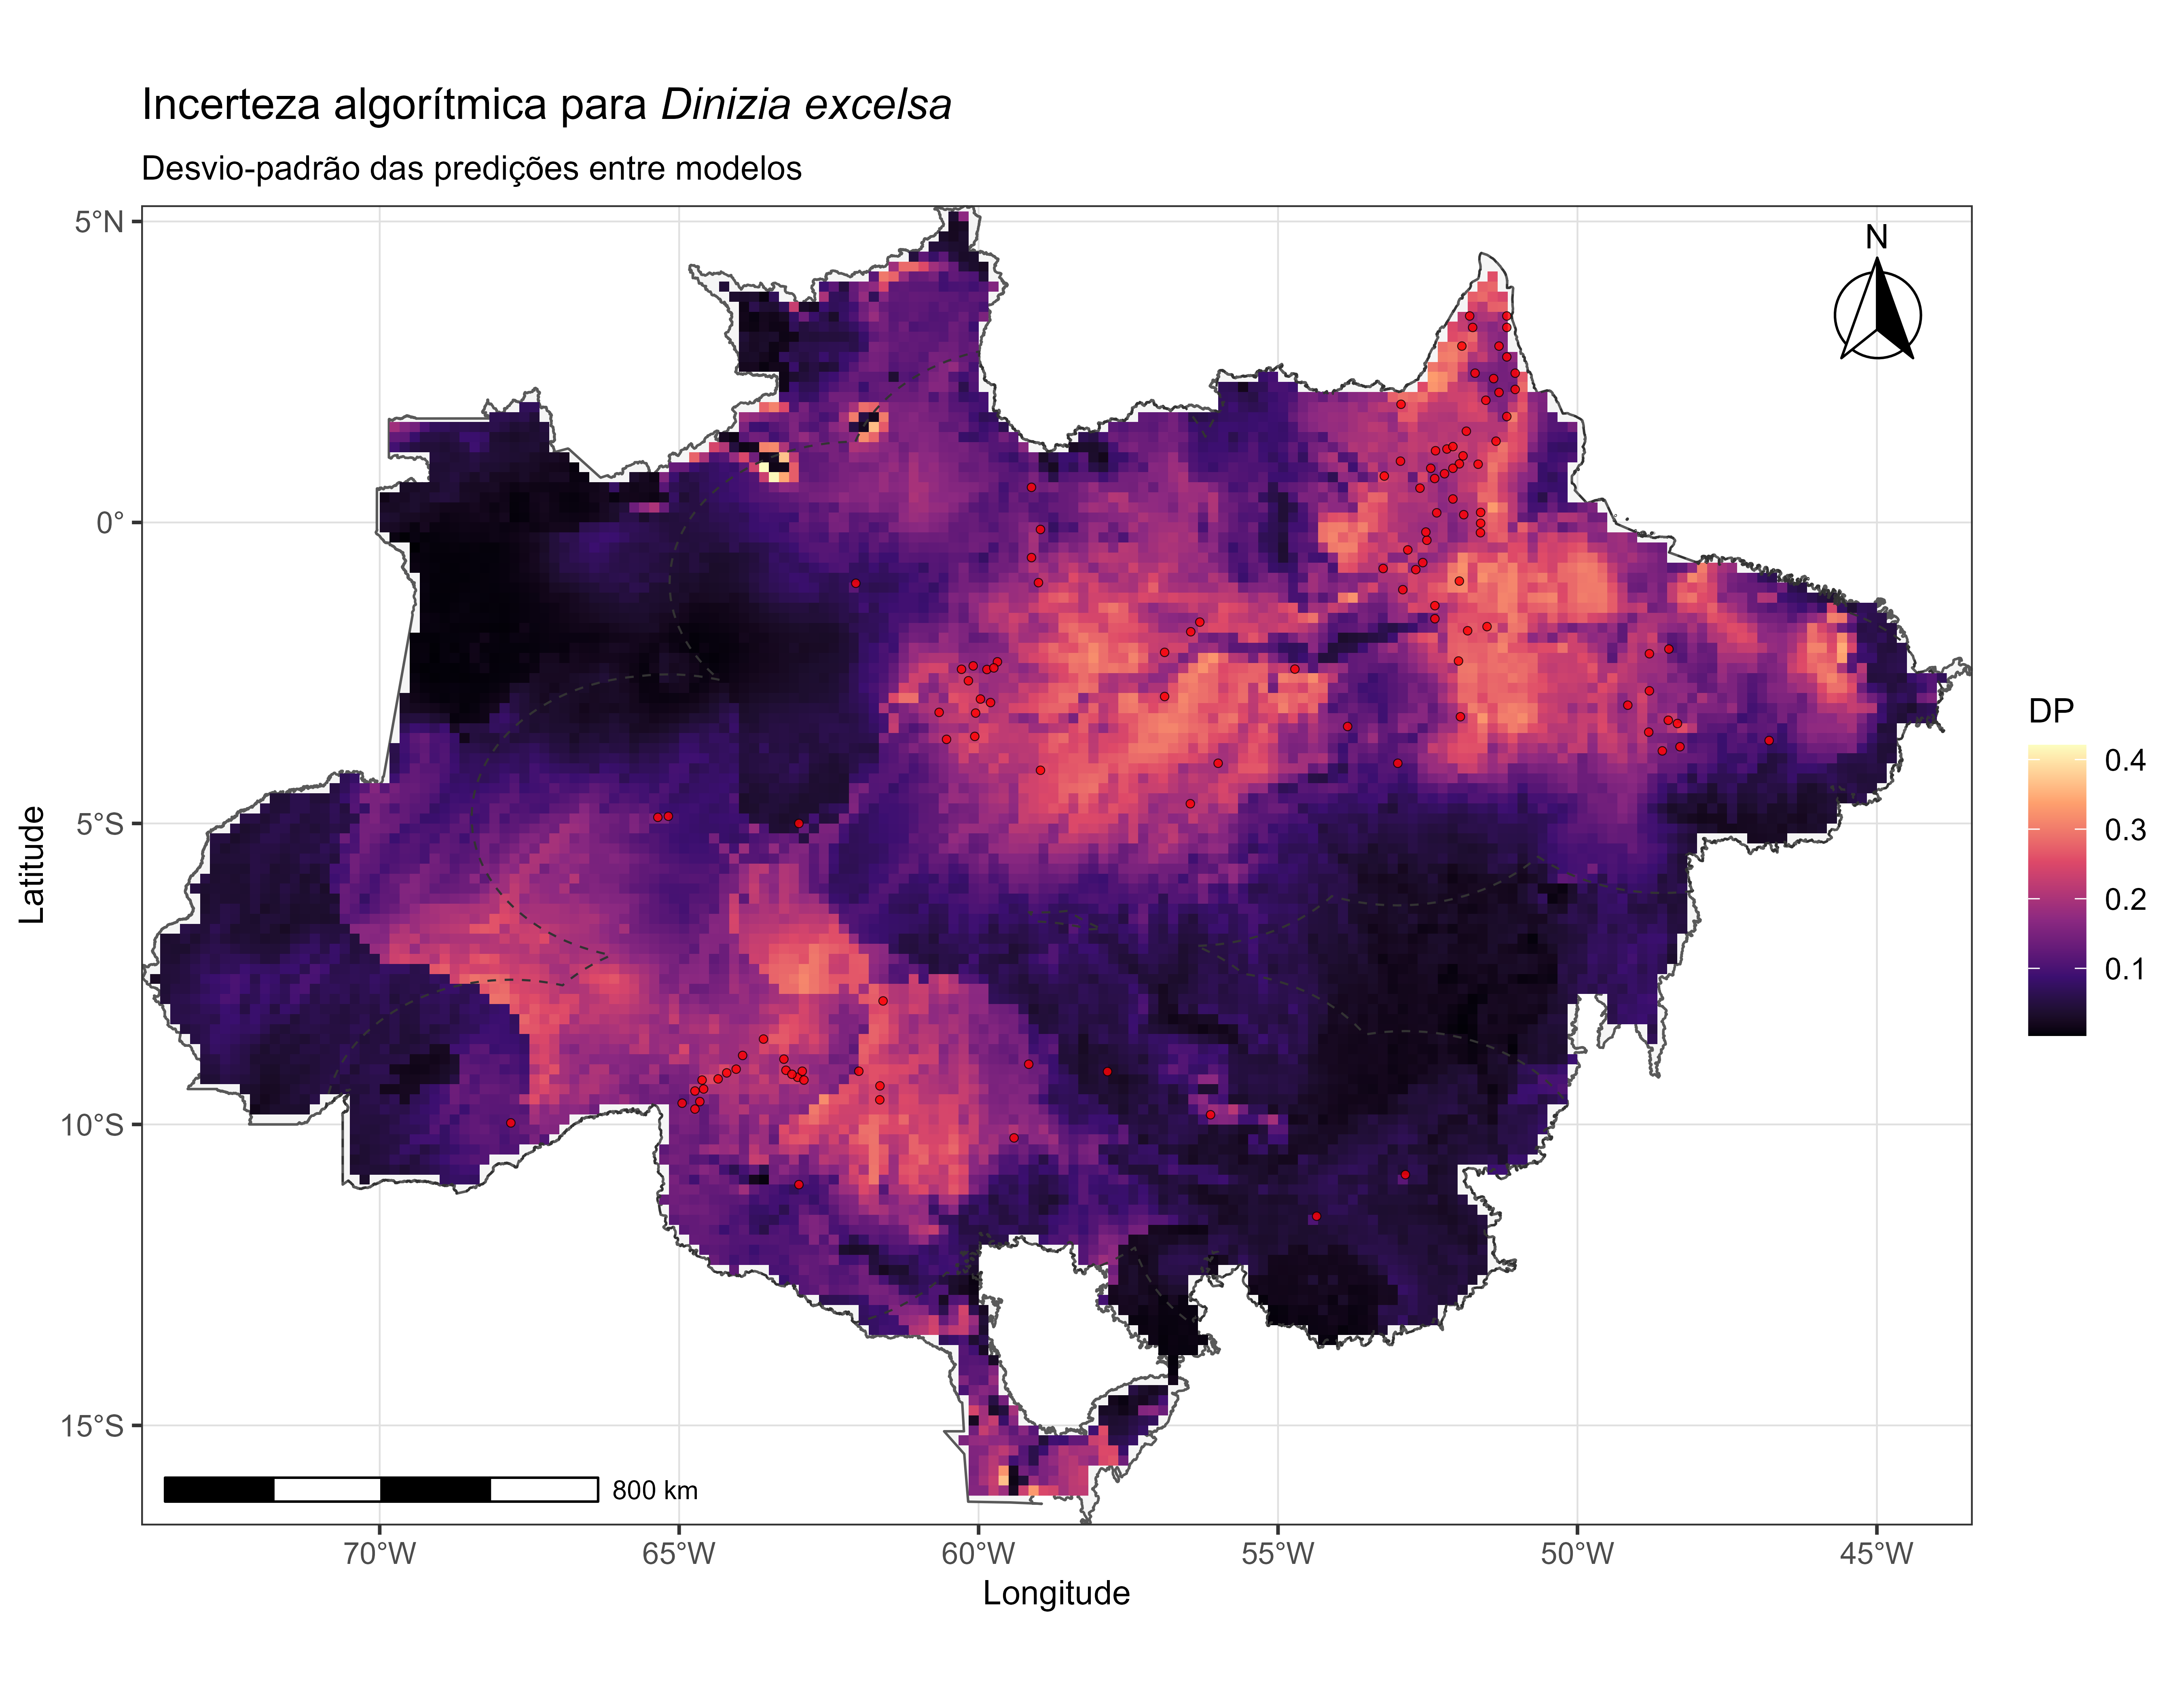
\includegraphics[width=0.88\textwidth]{figuras/unidade11/unidade11_incerteza_algoritmica.png}
\caption{Algorithmic disagreement summarized as the standard deviation among model predictions.}
\label{fig:unidade11_incerteza_algoritmica}
\end{figure}

\section{Integrated Comparison}
\rscriptfile{scripts/unidade11/07_comparacao_ensemble_modelos.R}
\begin{figure}[H]
\centering
\includegraphics[width=0.98\textwidth]{figuras/unidade11/unidade11_comparacao_ensemble.png}
\caption{Comparison of individual models, unweighted and weighted ensembles, binary consensus, and algorithmic disagreement.}
\label{fig:unidade11_comparacao_ensemble}
\end{figure}

\section{Complete Pipeline}
\rscriptfile{scripts/unidade11/08_pipeline_ensemble.R}

\section{Chapter Summary}
For \textit{Dinizia excelsa}, the ensemble integrates interpretable statistical
models and flexible algorithms to summarize present potential suitability
within $M$.
\begin{conceito}[title={\faBook\quad Key message}]
An ensemble does not replace critical evaluation of its components. Interpret
it together with evaluation metrics, response curves, ecological coherence,
and disagreement maps.
\end{conceito}

\section{Review Exercises}
\begin{enumerate}
\item Why are ensembles used in SDM?
\item Distinguish unweighted mean, weighted mean, and binary consensus.
\item Why should poor models be excluded?
\item How can algorithmic disagreement be mapped?
\item Why does a weighted ensemble depend on the selected metric?
\item How should high suitability with strong algorithmic disagreement be interpreted?
\item How can ensembles support future climate projections?
\end{enumerate}

\chapter[Model Evaluation]{Model Evaluation}

\begin{objetivos}
By the end of this chapter, readers should be able to:
\begin{itemize}
\item distinguish fit, discrimination, calibration, and transferability;
\item explain why random partitions may be optimistic;
\item choose among random, spatial, environmental, and independent validation;
\item interpret AUC, TSS, Kappa, sensitivity, specificity, and Boyce Index;
\item critically evaluate thresholds and binary maps; and
\item compare models without reducing the decision to a metric ranking.
\end{itemize}
\end{objetivos}

\section{Introduction}

Model evaluation is essential in SDM. A visually plausible map may still have
weak discrimination, sensitivity, specificity, or independence from calibration
data. Whenever possible, models should be evaluated using independent data
\parencite{fielding1997review,allouche2006assessing,hirzel2006evaluating,li2013thresholds,guisan2017habitat}.
Here, GLM, GAM, Random Forest, BRT, Maxent, and Ensemble predictions for
\textit{Dinizia excelsa} are compared to understand their performance,
limitations, and ecological coherence rather than automatically select the
largest metric.

\begin{conceito}[title={\faBook\quad Evaluation is not merely ranking}]
A useful SDM requires predictive performance, ecological coherence,
interpretable responses, and spatial or temporal generalization. The largest
AUC alone is not a sufficient decision rule.
\end{conceito}

\section{What Does It Mean to Evaluate an SDM?}

Evaluation confronts predictions with data not used to estimate model
parameters. Four questions follow. Does the model rank presences above absences
or background? When probabilistic interpretation is justified, do predicted
values agree with observed frequencies? Does error remain acceptable in a new
region, period, or environmental domain? Does the test design represent the
intended model use?

These questions concern \textbf{discrimination}, \textbf{calibration},
\textbf{transferability}, and \textbf{alignment between validation design and
prediction objective}. Good discrimination can coexist with poor calibration;
strong interpolation can coexist with failed transfer
\parencite{vaughan2005testing,jimenezvalverde2013discrimination,roberts2017crossvalidation}.

\begin{atencao}[title={\faExclamationTriangle\quad Suitability is not automatically probability}]
Probabilistic calibration is meaningful only when model output and sampling
design support occurrence or occupancy probability. Presence--background scores
do not become probabilities merely because they range from zero to one.
\end{atencao}

\section{Random Validation and Spatial Dependence}

Random cross-validation can place nearby records in training and test sets.
Neighboring locations often share climate, soil, sampling history, and residual
autocorrelation, making the test artificially easy and error estimates
optimistic \parencite{roberts2017crossvalidation}. This is particularly relevant
for Amazonian records clustered along rivers, roads, cities, and historically
surveyed sites.

\begin{conceito}[title={\faBook\quad Spatial leakage}]
Spatial leakage occurs when proximity, dependence, or shared sampling units let
training information make the test set artificially easy. A formally distinct
test record may still fail to provide independent information.
\end{conceito}

\section{Partitioning Strategies}

\subsection{Random Cross-Validation}
Useful for diagnosing fit within the sampled domain and comparing implementations
under a common split, but insufficient evidence of spatial transfer for
structured data.

\subsection{Spatial Blocks}
Whole geographic blocks are assigned to training or testing. Block size should
reflect autocorrelation, occurrence density, and prediction distance. Blocks
that are too small retain dependence; overly large blocks yield few,
imbalanced folds and variable error estimates
\parencite{roberts2017crossvalidation,valavi2019blockcv}.

\subsection{Buffering and Distance Separation}
Buffers exclude training records near test points and directly impose a minimum
calibration--evaluation distance, at the cost of smaller training sets and
potentially greater fold-to-fold variability.

\subsection{Environmental Blocking}
Records are grouped in environmental space, for example by clustering continuous
predictors. This tests transfer to environmental combinations not represented in
training and answers a different question from geographic blocking
\parencite{valavi2019blockcv}.

\subsection{Independent Validation}
Data from another campaign, region, or period provide the most direct test of
the corresponding transfer, provided definitions, effort, and detectability are
comparable. Geographic independence alone does not correct protocol differences.

\begin{atencao}[title={\faExclamationTriangle\quad No partition is universally best}]
The strategy must emulate intended use. Landscape interpolation, geographic
transfer, and future climate projection are different problems requiring
different tests.
\end{atencao}

\section{Reproducible Spatial Folds}

For \textit{Dinizia excelsa}, presences and background are linked to a grid in a
metric projection. Whole cells, not individual records, are assigned to folds.
Every fold must retain both classes, and spatial separation must represent a
relevant prediction distance.

\begin{rcode}
# Run from the project root
source("scripts/unidade12/09_criar_folds_espaciais.R")
source("scripts/unidade12/10_validacao_espacial_glm.R")
\end{rcode}
\rscriptref{scripts/unidade12/09_criar_folds_espaciais.R}
\rscriptref{scripts/unidade12/10_validacao_espacial_glm.R}

The first script writes fold assignments, the spatial grid, and a diagnostic
map. The second recalculates predictor standardization using training data only,
refits the GLM in each fold, and computes AUC, TSS, sensitivity, specificity,
and Brier score. Reusing means and standard deviations calculated from all
records would constitute preprocessing leakage.

\begin{atencao}[title={\faExclamationTriangle\quad Block size is not a decorative hyperparameter}]
The initial 300-km value is an explicit diagnostic setting, not a universal
recommendation. Final analysis should justify distance using the question's
scale, sampling pattern, autocorrelation, and transfer horizon.
\end{atencao}

\begin{figure}[htbp]
\centering
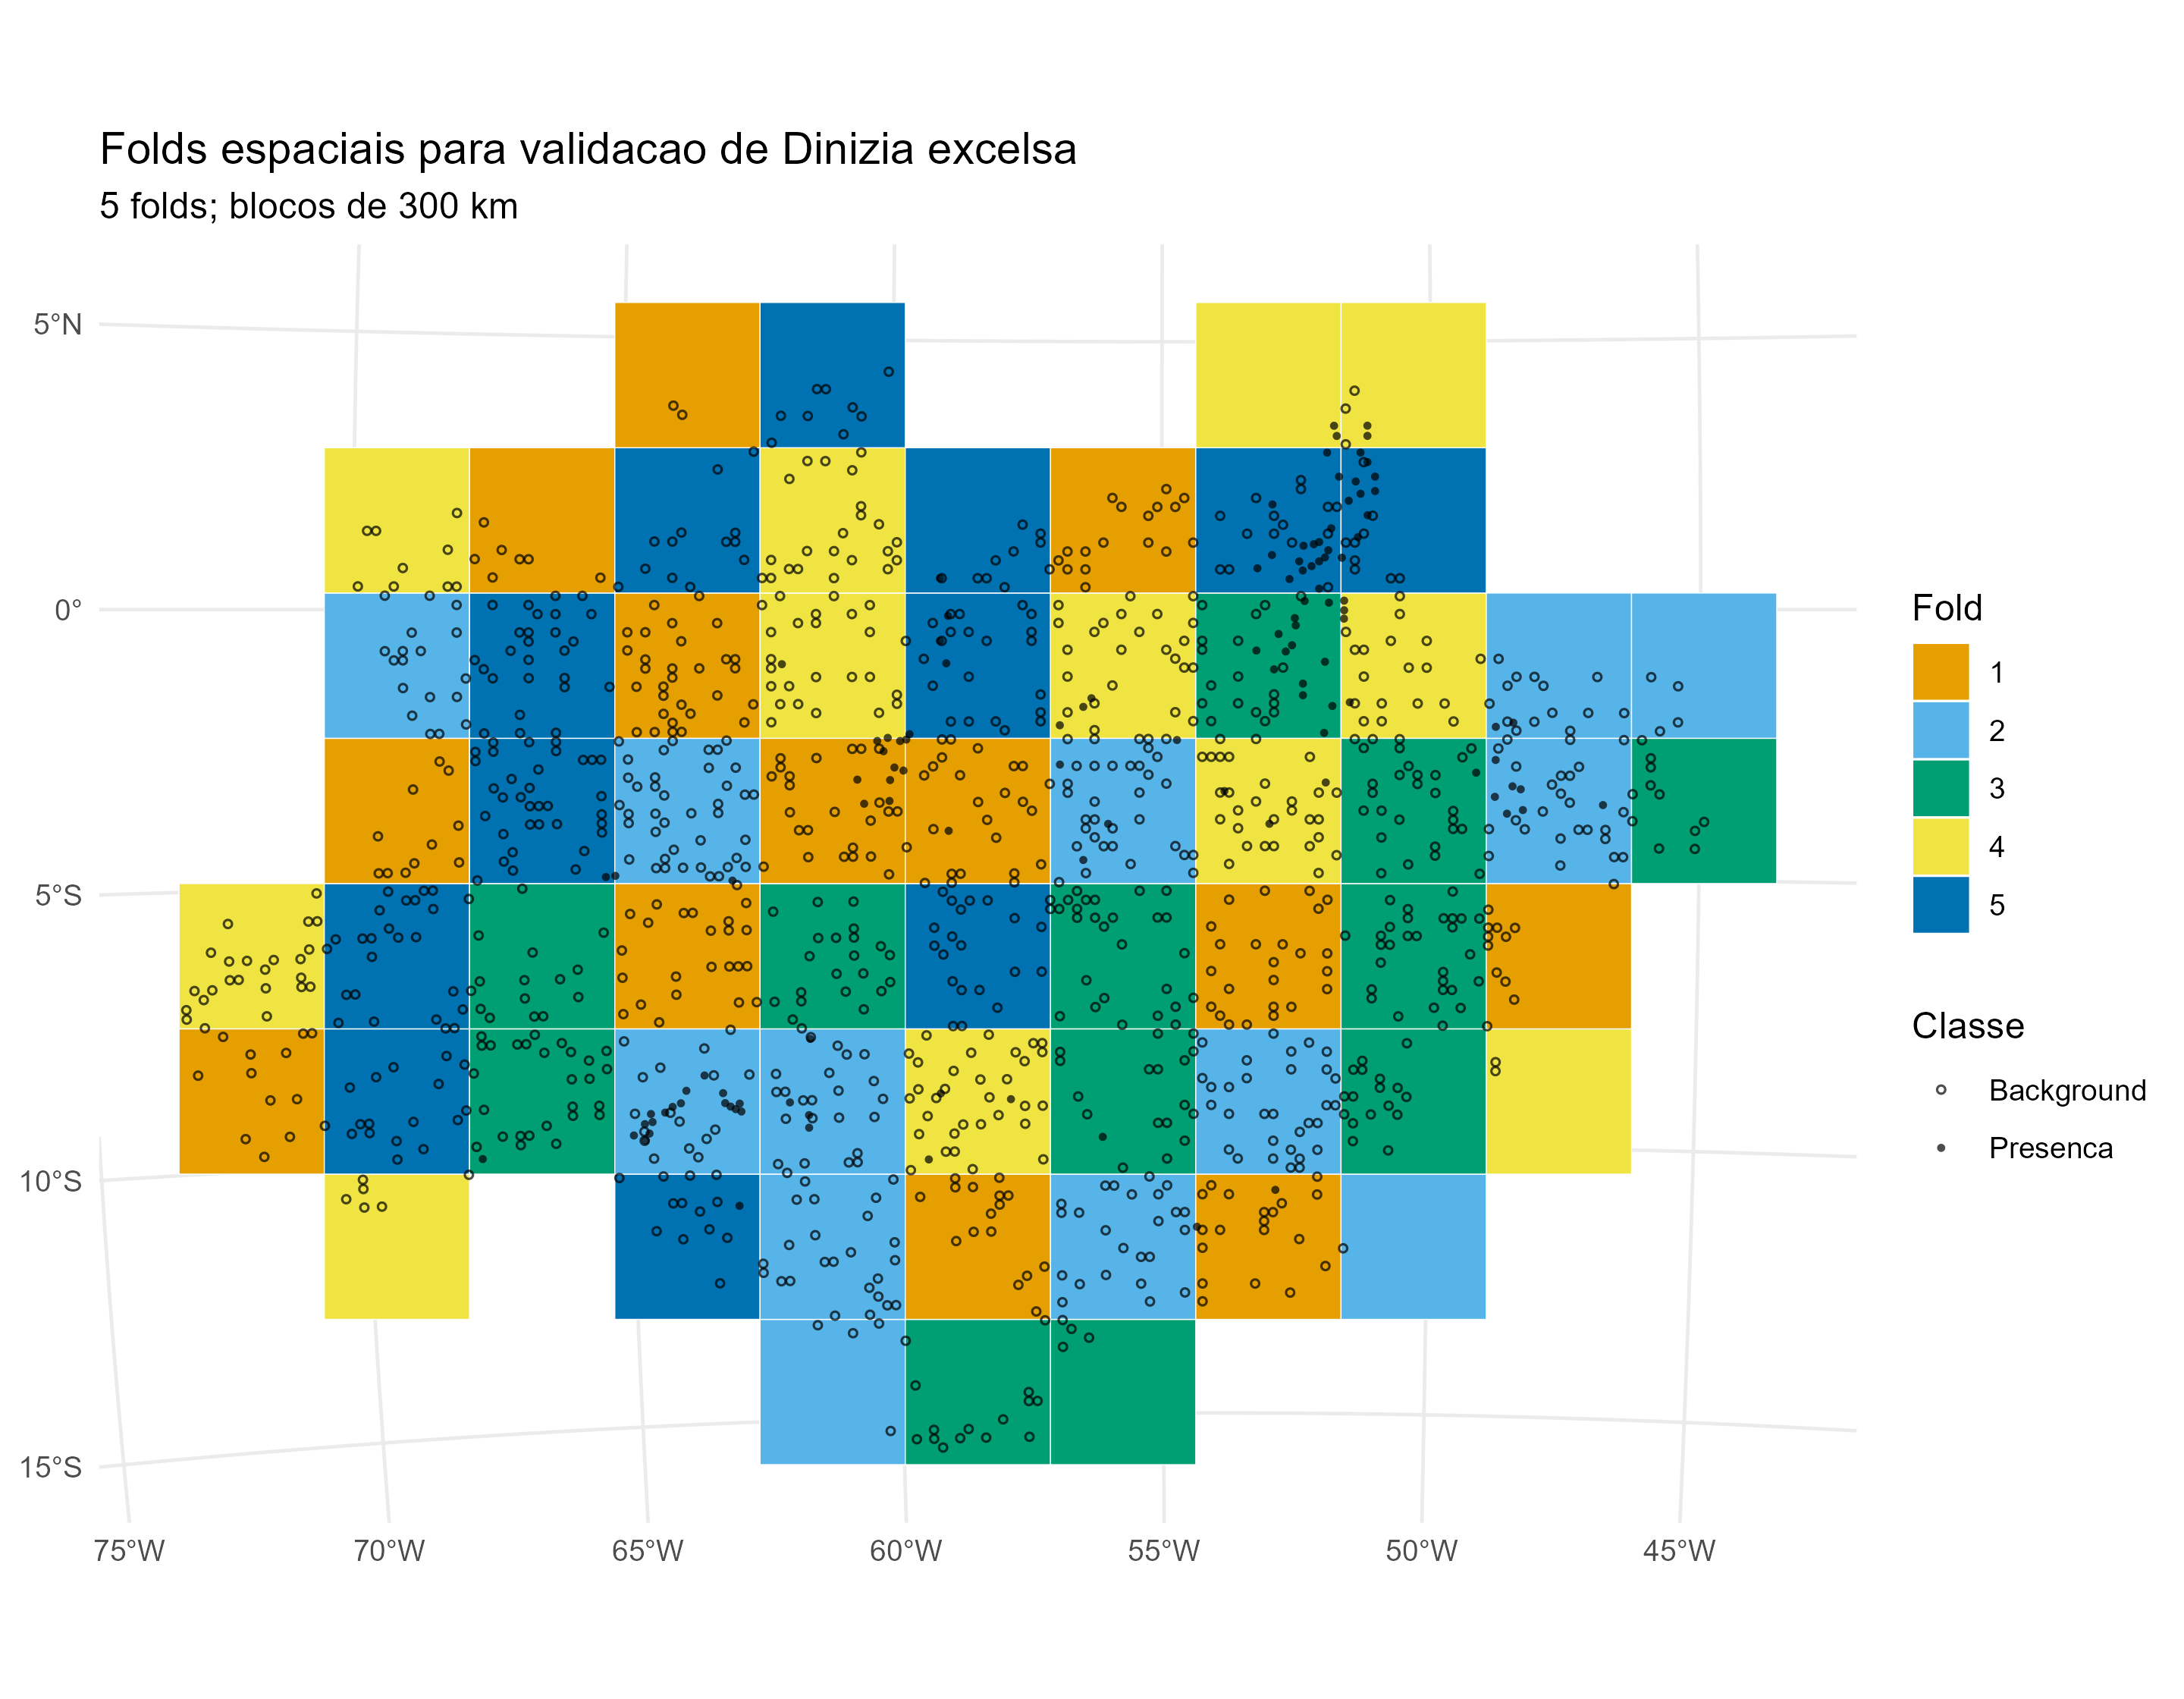
\includegraphics[width=0.93\textwidth]{figuras/unidade12/unidade12_folds_espaciais.png}
\caption{Reproducible spatial partition used for diagnosis. Each 300-km cell belongs entirely to one of five folds; filled circles are presences and open circles are background. Cells from one fold may be dispersed, so this configuration does not impose an exclusion buffer between training and testing.}
\label{fig:unidade12-folds-espaciais}
\end{figure}

\subsection{Spatial Diagnostic Results}
All folds retained presences and background. The GLM converged in all refits,
but AUC ranged from 0.643 to 0.851 and specificity from 0.475 to 0.829. This
variation is more informative than a single average because it reveals unstable
regional transfer.

\begin{table}[htbp]
\centering
\caption{GLM performance across five spatial folds. Mean and standard deviation (SD) summarize independent refits.}
\label{tab:unidade12-validacao-espacial}
\begin{tabular}{lrrr}
\toprule
Metric & Mean & SD & Range \\
\midrule
AUC & 0.779 & 0.082 & 0.643--0.851 \\
TSS & 0.528 & 0.093 & 0.419--0.658 \\
Sensitivity & 0.826 & 0.132 & 0.632--0.944 \\
Specificity & 0.703 & 0.155 & 0.475--0.829 \\
Brier & 0.078 & 0.030 & 0.043--0.116 \\
\bottomrule
\end{tabular}
\end{table}

\begin{figure}[htbp]
\centering
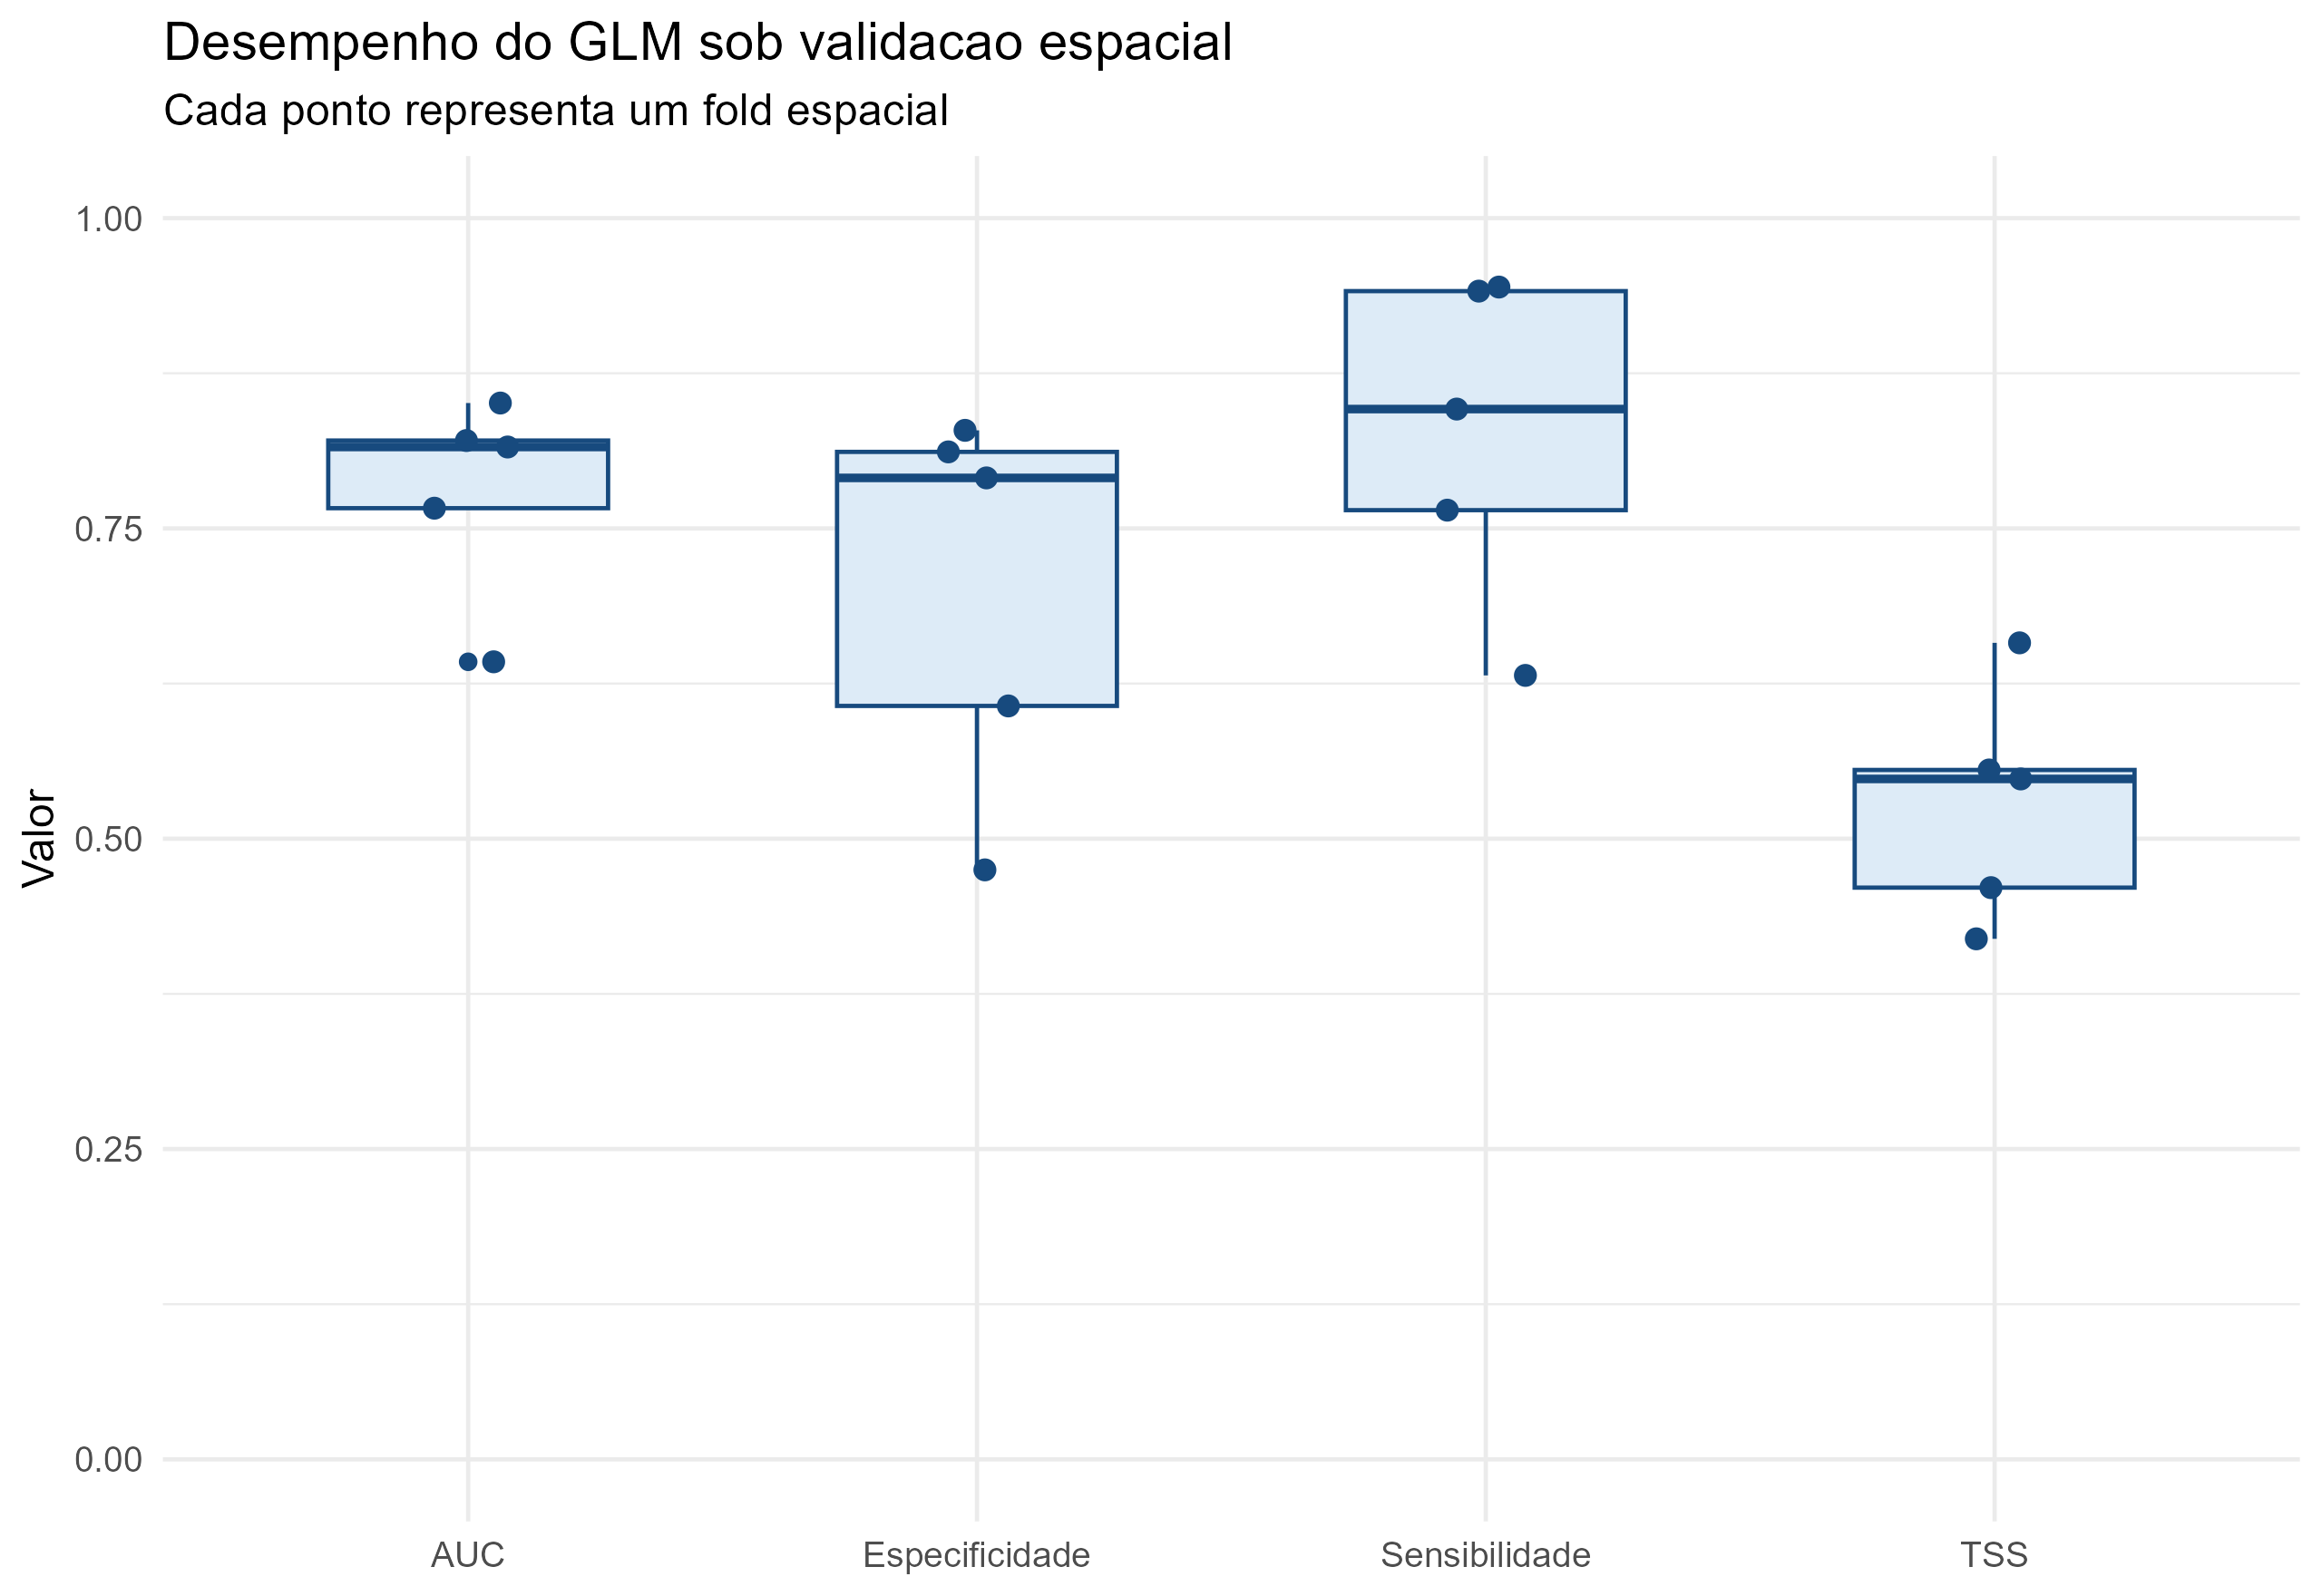
\includegraphics[width=0.88\textwidth]{figuras/unidade12/unidade12_validacao_espacial_glm.png}
\caption{Variation in GLM metrics among five spatial folds. Points are fold-specific results; the box is only a visual summary and does not replace inspection of individual values.}
\label{fig:unidade12-desempenho-espacial}
\end{figure}

The fits warned of probabilities numerically near zero or one. Although all
converged, 37 test predictions were extreme under the operational criterion
$\hat p\leq10^{-6}$ or $\hat p\geq1-10^{-6}$. This may indicate separation,
extrapolation, or excessive flexibility in quadratic terms and must be examined
before interpreting scores as calibrated probabilities. The results alone do
not establish superiority or inferiority relative to random validation; such a
comparison must hold model, data, preprocessing, and metrics constant.

\section{Spatial Sorting Bias}
Spatial sorting bias occurs when test presences are closer to training presences
than evaluation absences or background are. Even a geographic-distance-only
model may then achieve high AUC. Training--test distance inspection and null
models help reveal this bias \parencite{hijmans2012spatialsorting}.

\begin{decisao}[title={\faRoute\quad Methodological decision}]
Before calculating metrics, state whether the target is local interpolation,
geographic transfer, environmental transfer, or temporal projection. Construct
folds representing that prediction distance and use identical folds across
algorithms.
\end{decisao}

\section{Discrimination and Calibration}
Discrimination concerns ranking: do presences receive higher scores than
absences or background? Calibration concerns correspondence between predictions
and observed frequencies when such interpretation is valid. ROC curves and AUC
measure discrimination, not calibration. Reliability diagrams, calibration
intercept and slope, and proper scoring rules complement probabilistic evaluation
\parencite{vaughan2005testing,jimenezvalverde2013discrimination}.

\begin{conceito}[title={\faBalanceScale\quad A model can rank correctly but miss the magnitude}]
Models can rank sites similarly and have comparable AUC while producing values
with very different meanings and calibration. Discrimination does not authorize
interpreting suitability as occurrence probability.
\end{conceito}

\section{AUC and the ROC Curve}
The ROC curve relates sensitivity to $1-$specificity across thresholds. AUC is
the probability that a randomly selected presence receives a higher score than
a randomly selected background or absence:
\begin{equationbox}
\[AUC=P(\hat y_{presence}>\hat y_{background}).\]
\end{equationbox}
\begin{atencao}[title={\faExclamationTriangle\quad Limitations of AUC}]
With presence--background data, AUC depends on geographic extent, selected
background, sampling bias, and prevalence. A high value does not guarantee an
ecologically sound model.
\end{atencao}

\section{Sensitivity, Specificity, and TSS}
Sensitivity is the proportion of presences classified as suitable; specificity
is the proportion of absences or background classified as unsuitable.
\begin{equationbox}
\[Sensitivity=\frac{TP}{TP+FN}\]
\[Specificity=\frac{TN}{TN+FP}\]
\[TSS=Sensitivity+Specificity-1.\]
\end{equationbox}
TSS ranges from $-1$ to 1, with values nearer 1 indicating better binary discrimination.

\section{Kappa}
Kappa measures agreement between binary predictions and observations after
correcting for chance agreement, but is sensitive to prevalence and data distribution.
\begin{equationbox}
\[Kappa=\frac{p_o-p_e}{1-p_e},\]
\end{equationbox}
where $p_o$ is observed agreement and $p_e$ is chance-expected agreement.

\section{Boyce Index}
Boyce Index is useful for presence--background or presence-only models. It tests
whether presences occur preferentially where predicted suitability is higher
\parencite{hirzel2006evaluating}.
\begin{conceito}[title={\faBook\quad Boyce Index}]
Positive Boyce values indicate that presences concentrate in higher-suitability
classes, but the result depends on binning or smoothing choices and evaluation data.
\end{conceito}

\section{Integrated Evaluation Workflow}
\rscriptfile{scripts/unidade12/01_estrutura_pastas.R}
\rscriptfile{scripts/unidade12/02_preparar_predicoes_avaliacao.R}

\section{Calculating Metrics}
\rscriptfile{scripts/unidade12/03_calcular_metricas_modelos.R}
\begin{figure}[H]\centering
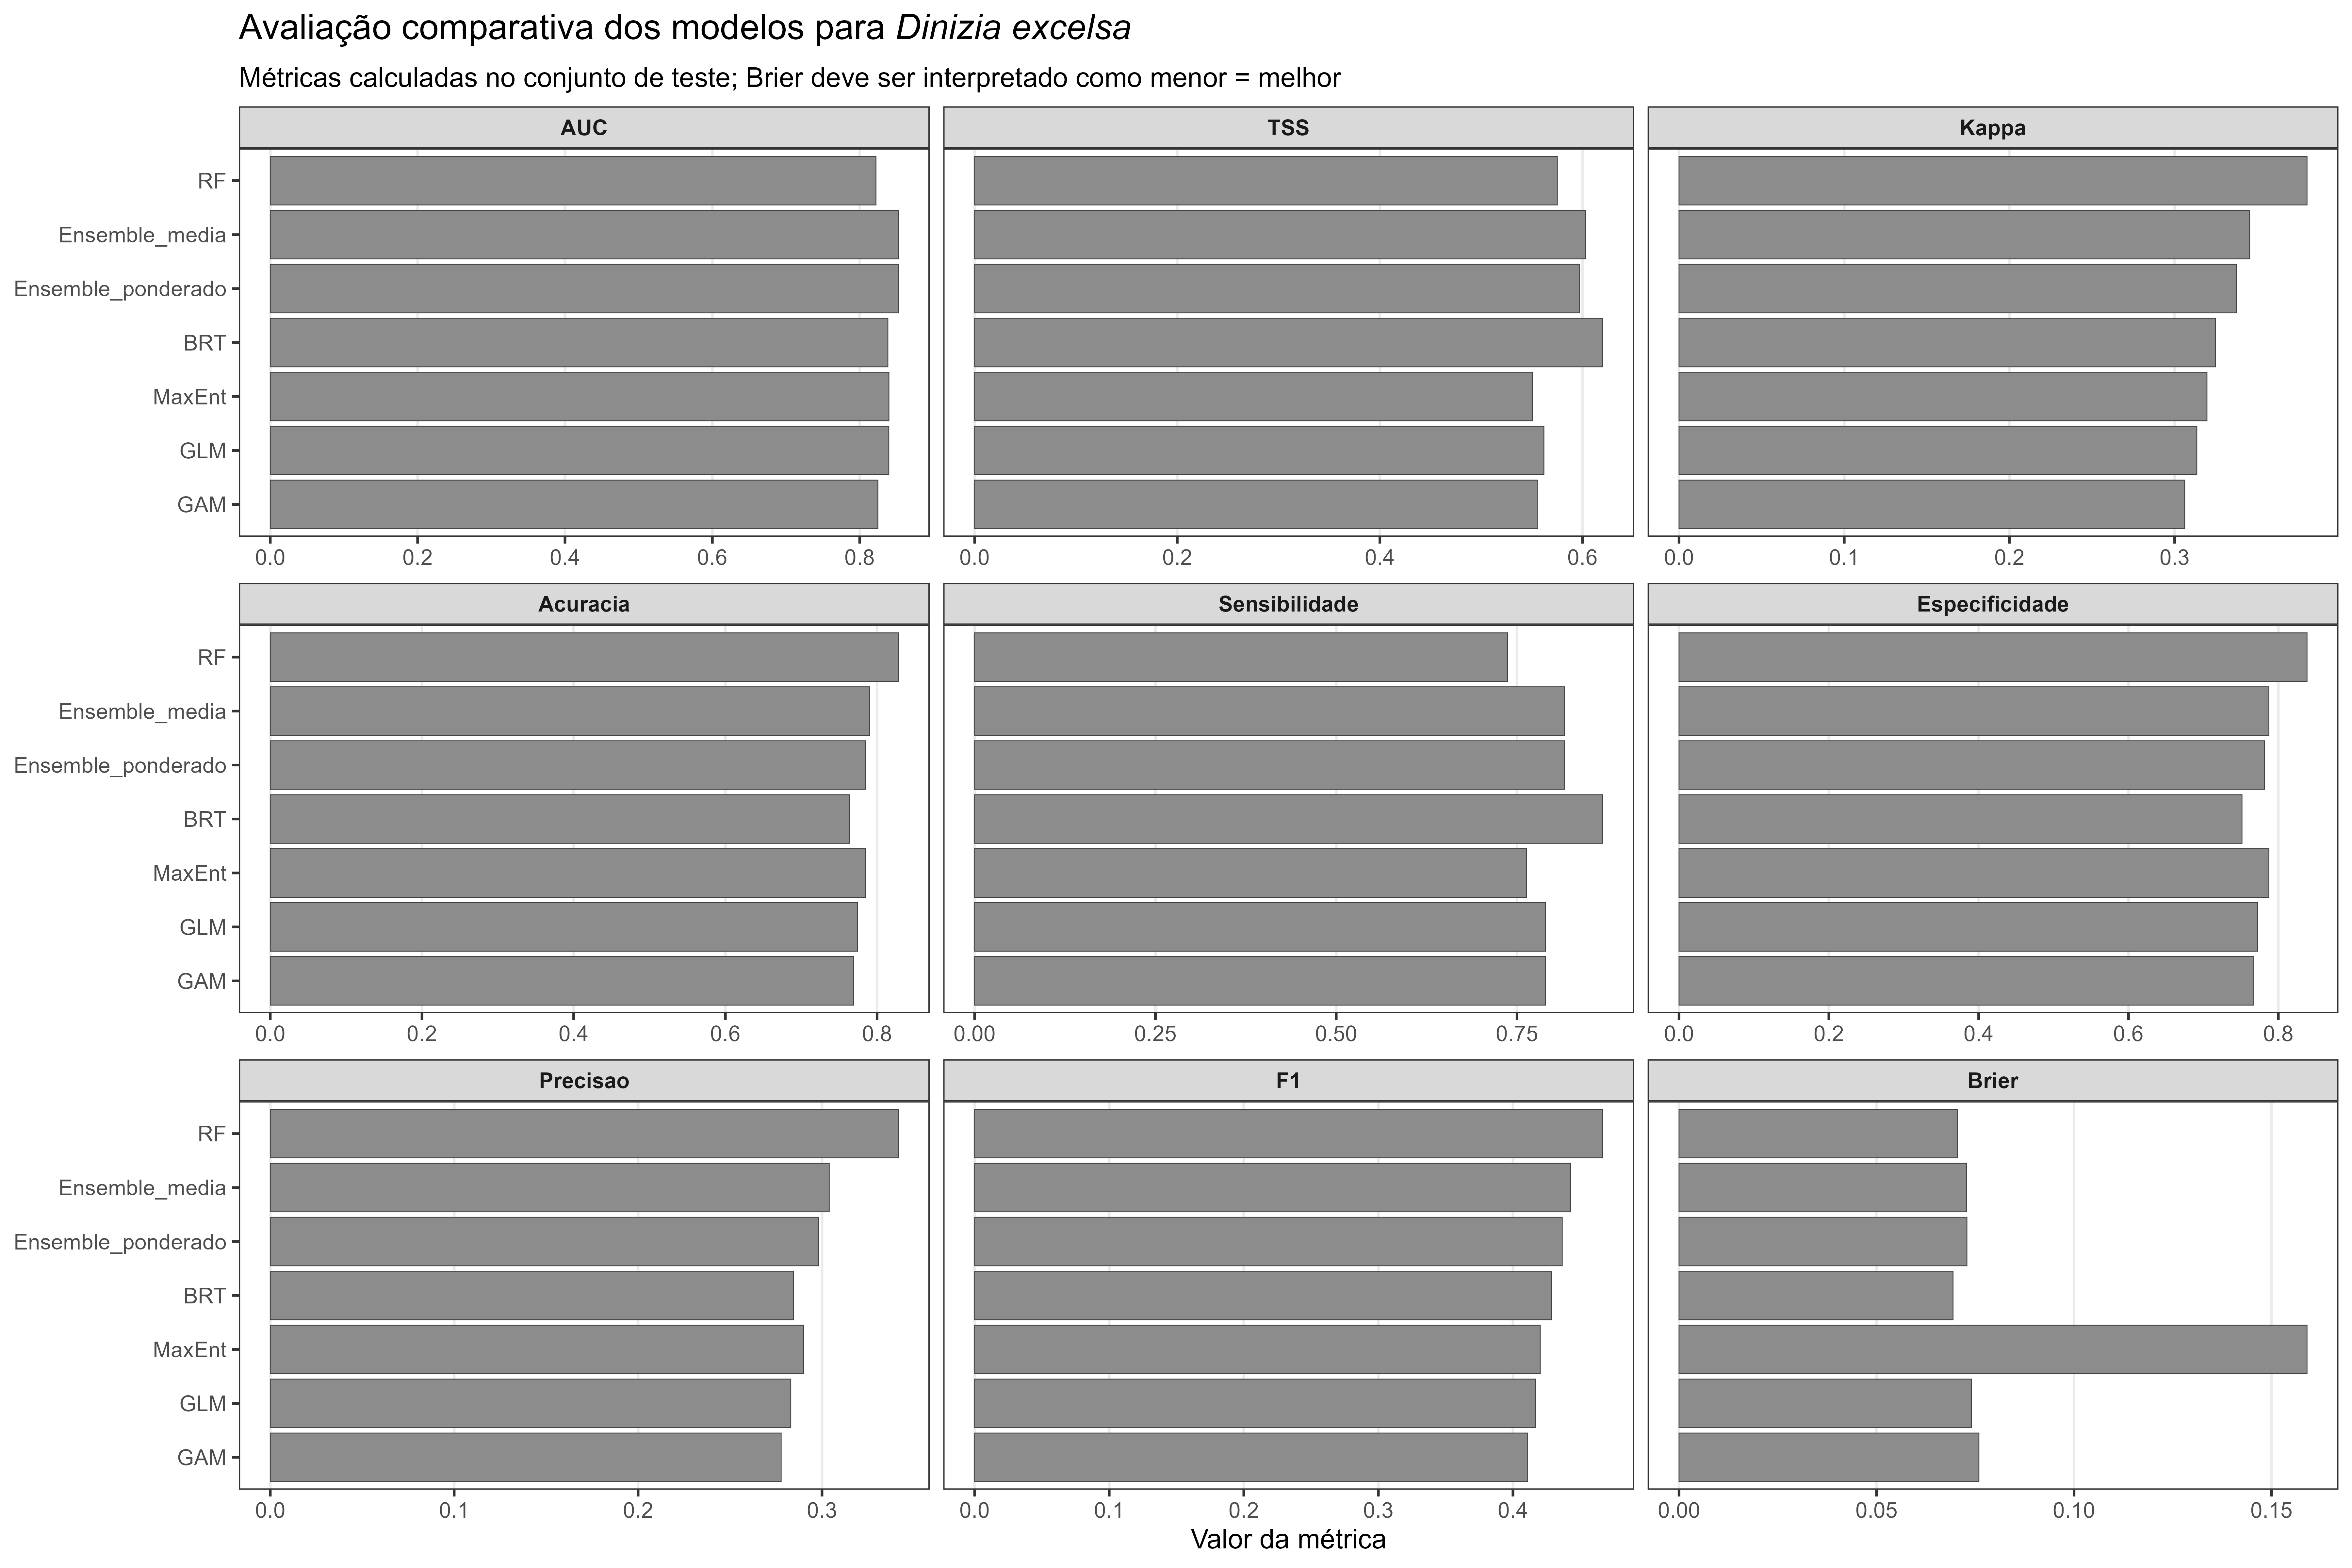
\includegraphics[width=0.95\textwidth]{figuras/unidade12/unidade12_comparacao_metricas.png}
\caption{Comparison of evaluation metrics for models fitted to \textit{Dinizia excelsa}.}\label{fig:unidade12_metricas}
\end{figure}

\section{Comparative ROC Curves}
\rscriptfile{scripts/unidade12/04_curvas_roc_comparativas.R}
\begin{figure}[H]\centering
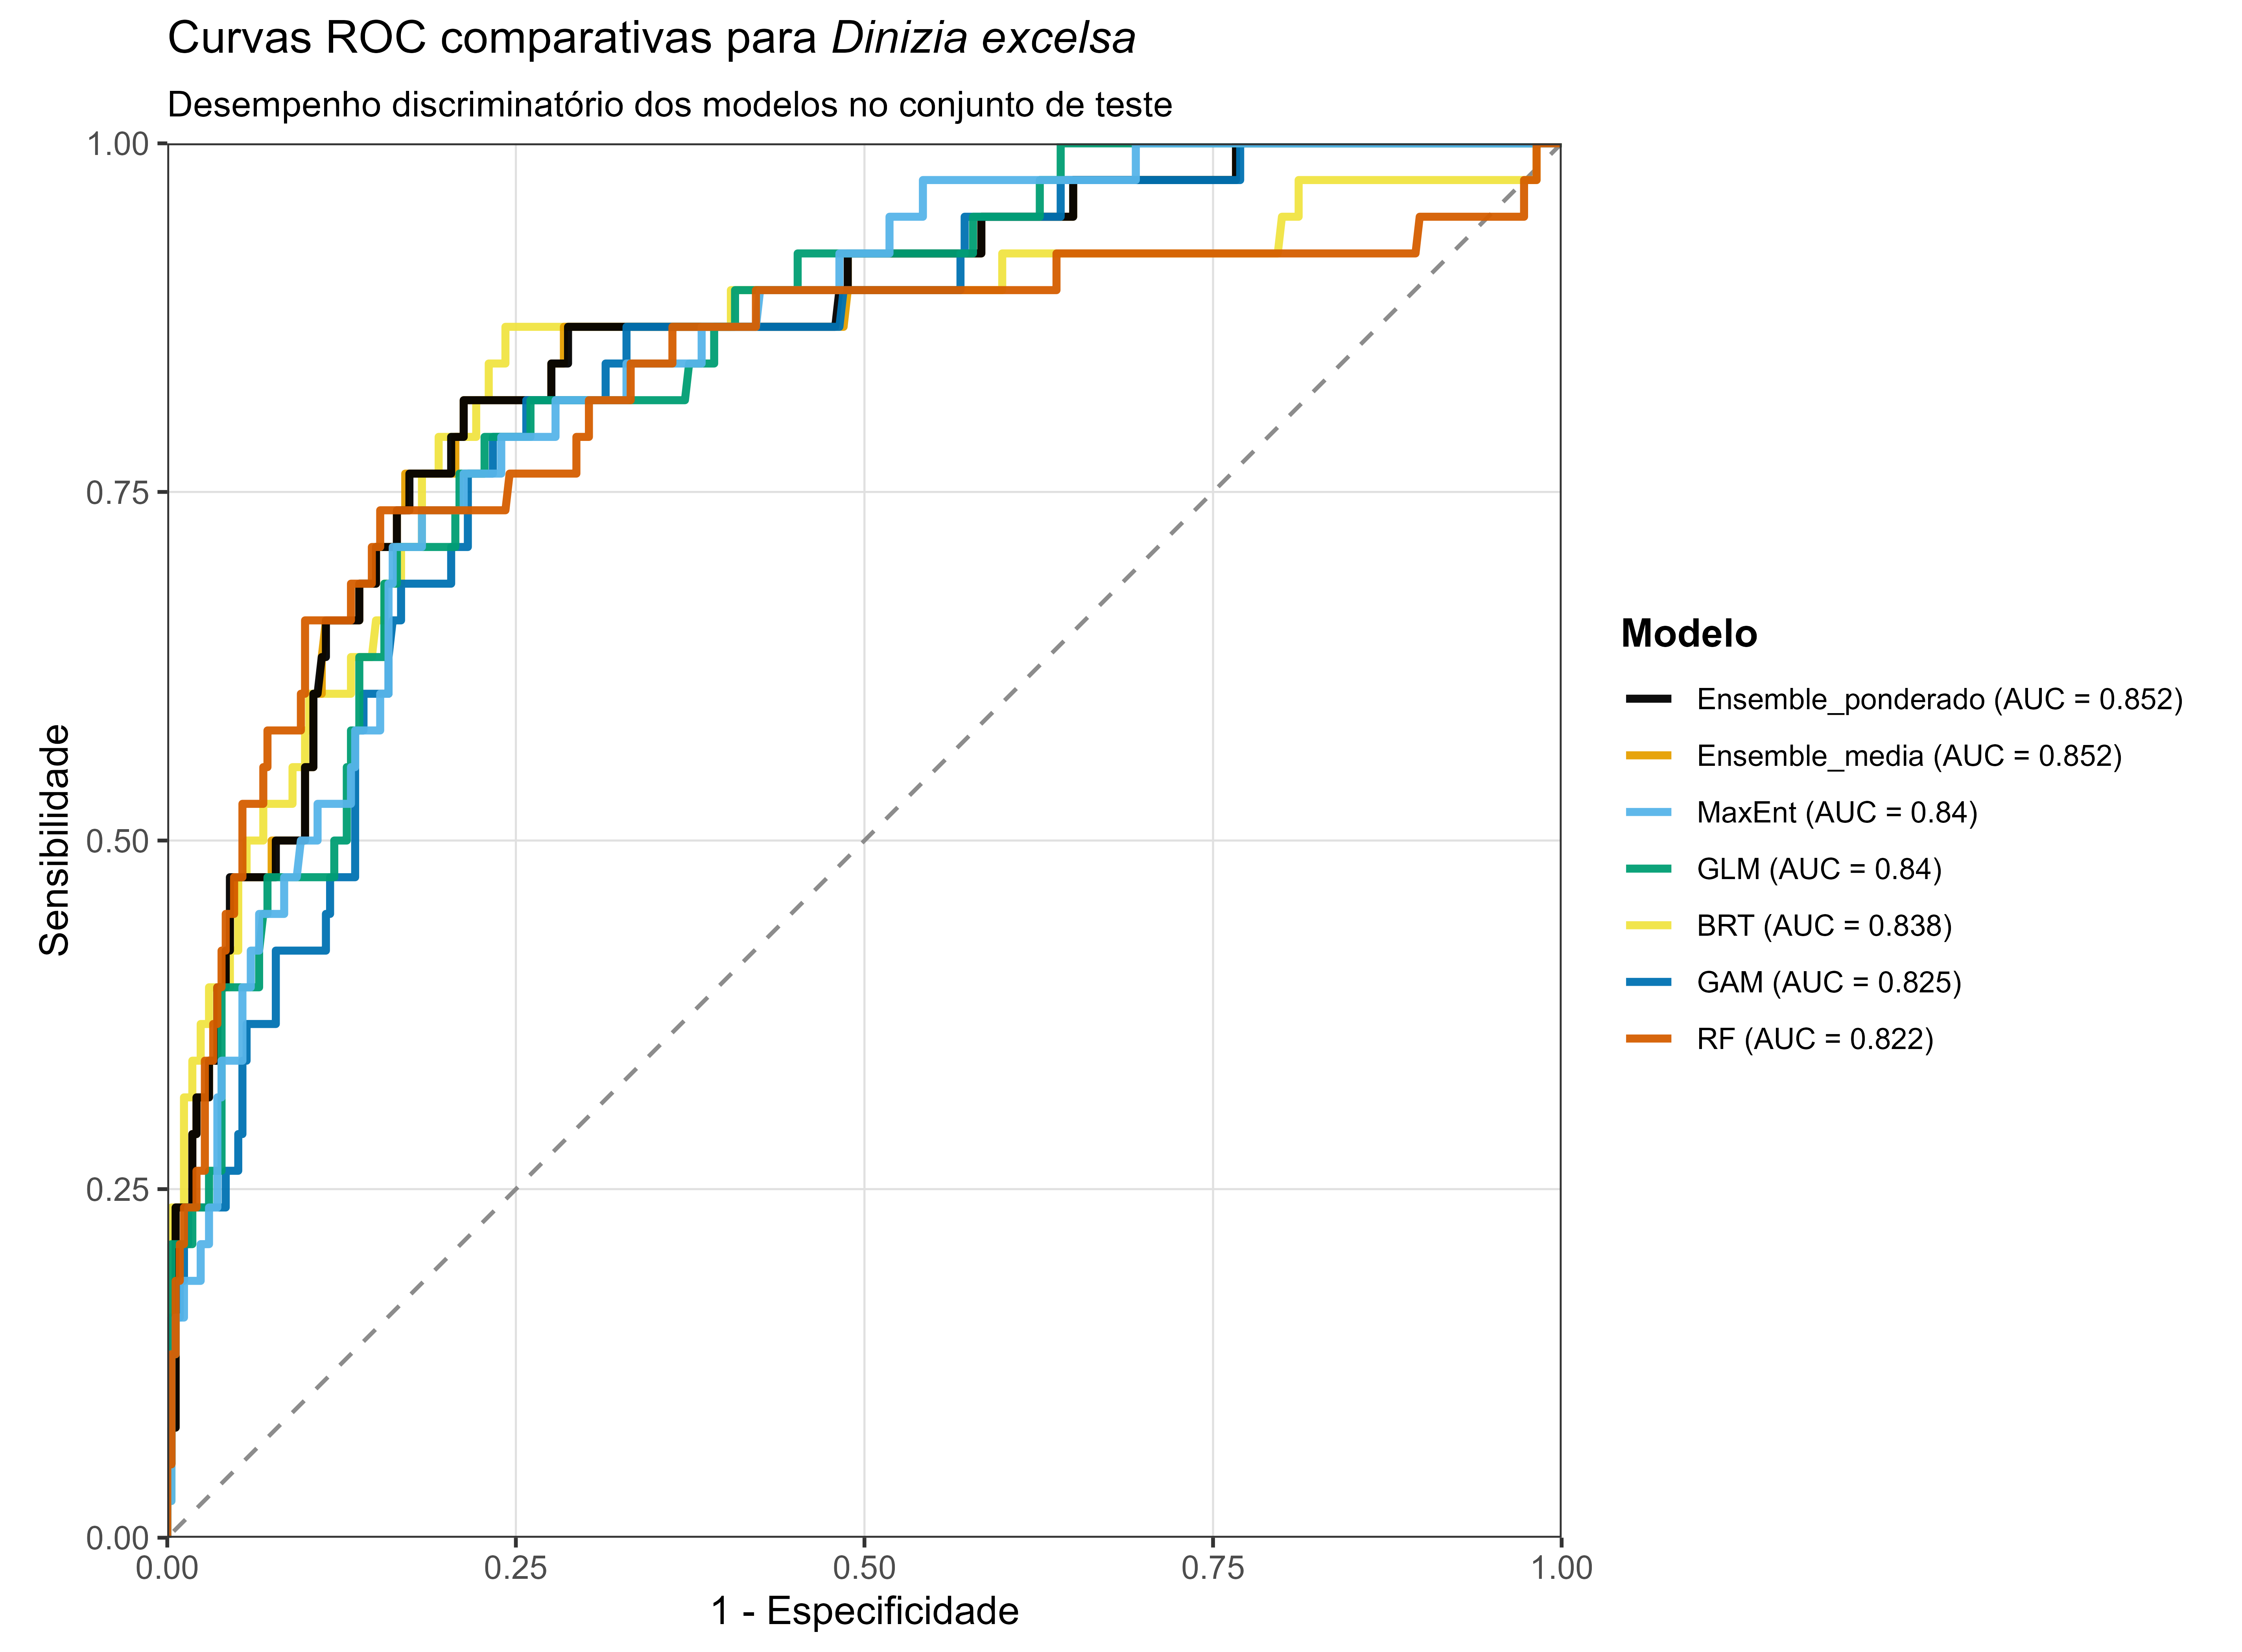
\includegraphics[width=0.86\textwidth]{figuras/unidade12/unidade12_curvas_roc_comparativas.png}
\caption{ROC curves for GLM, GAM, Random Forest, BRT, Maxent, and Ensemble.}\label{fig:unidade12_roc_comparativas}
\end{figure}

\section{Confusion Matrices}
\rscriptfile{scripts/unidade12/05_matrizes_confusao.R}
\begin{figure}[H]\centering
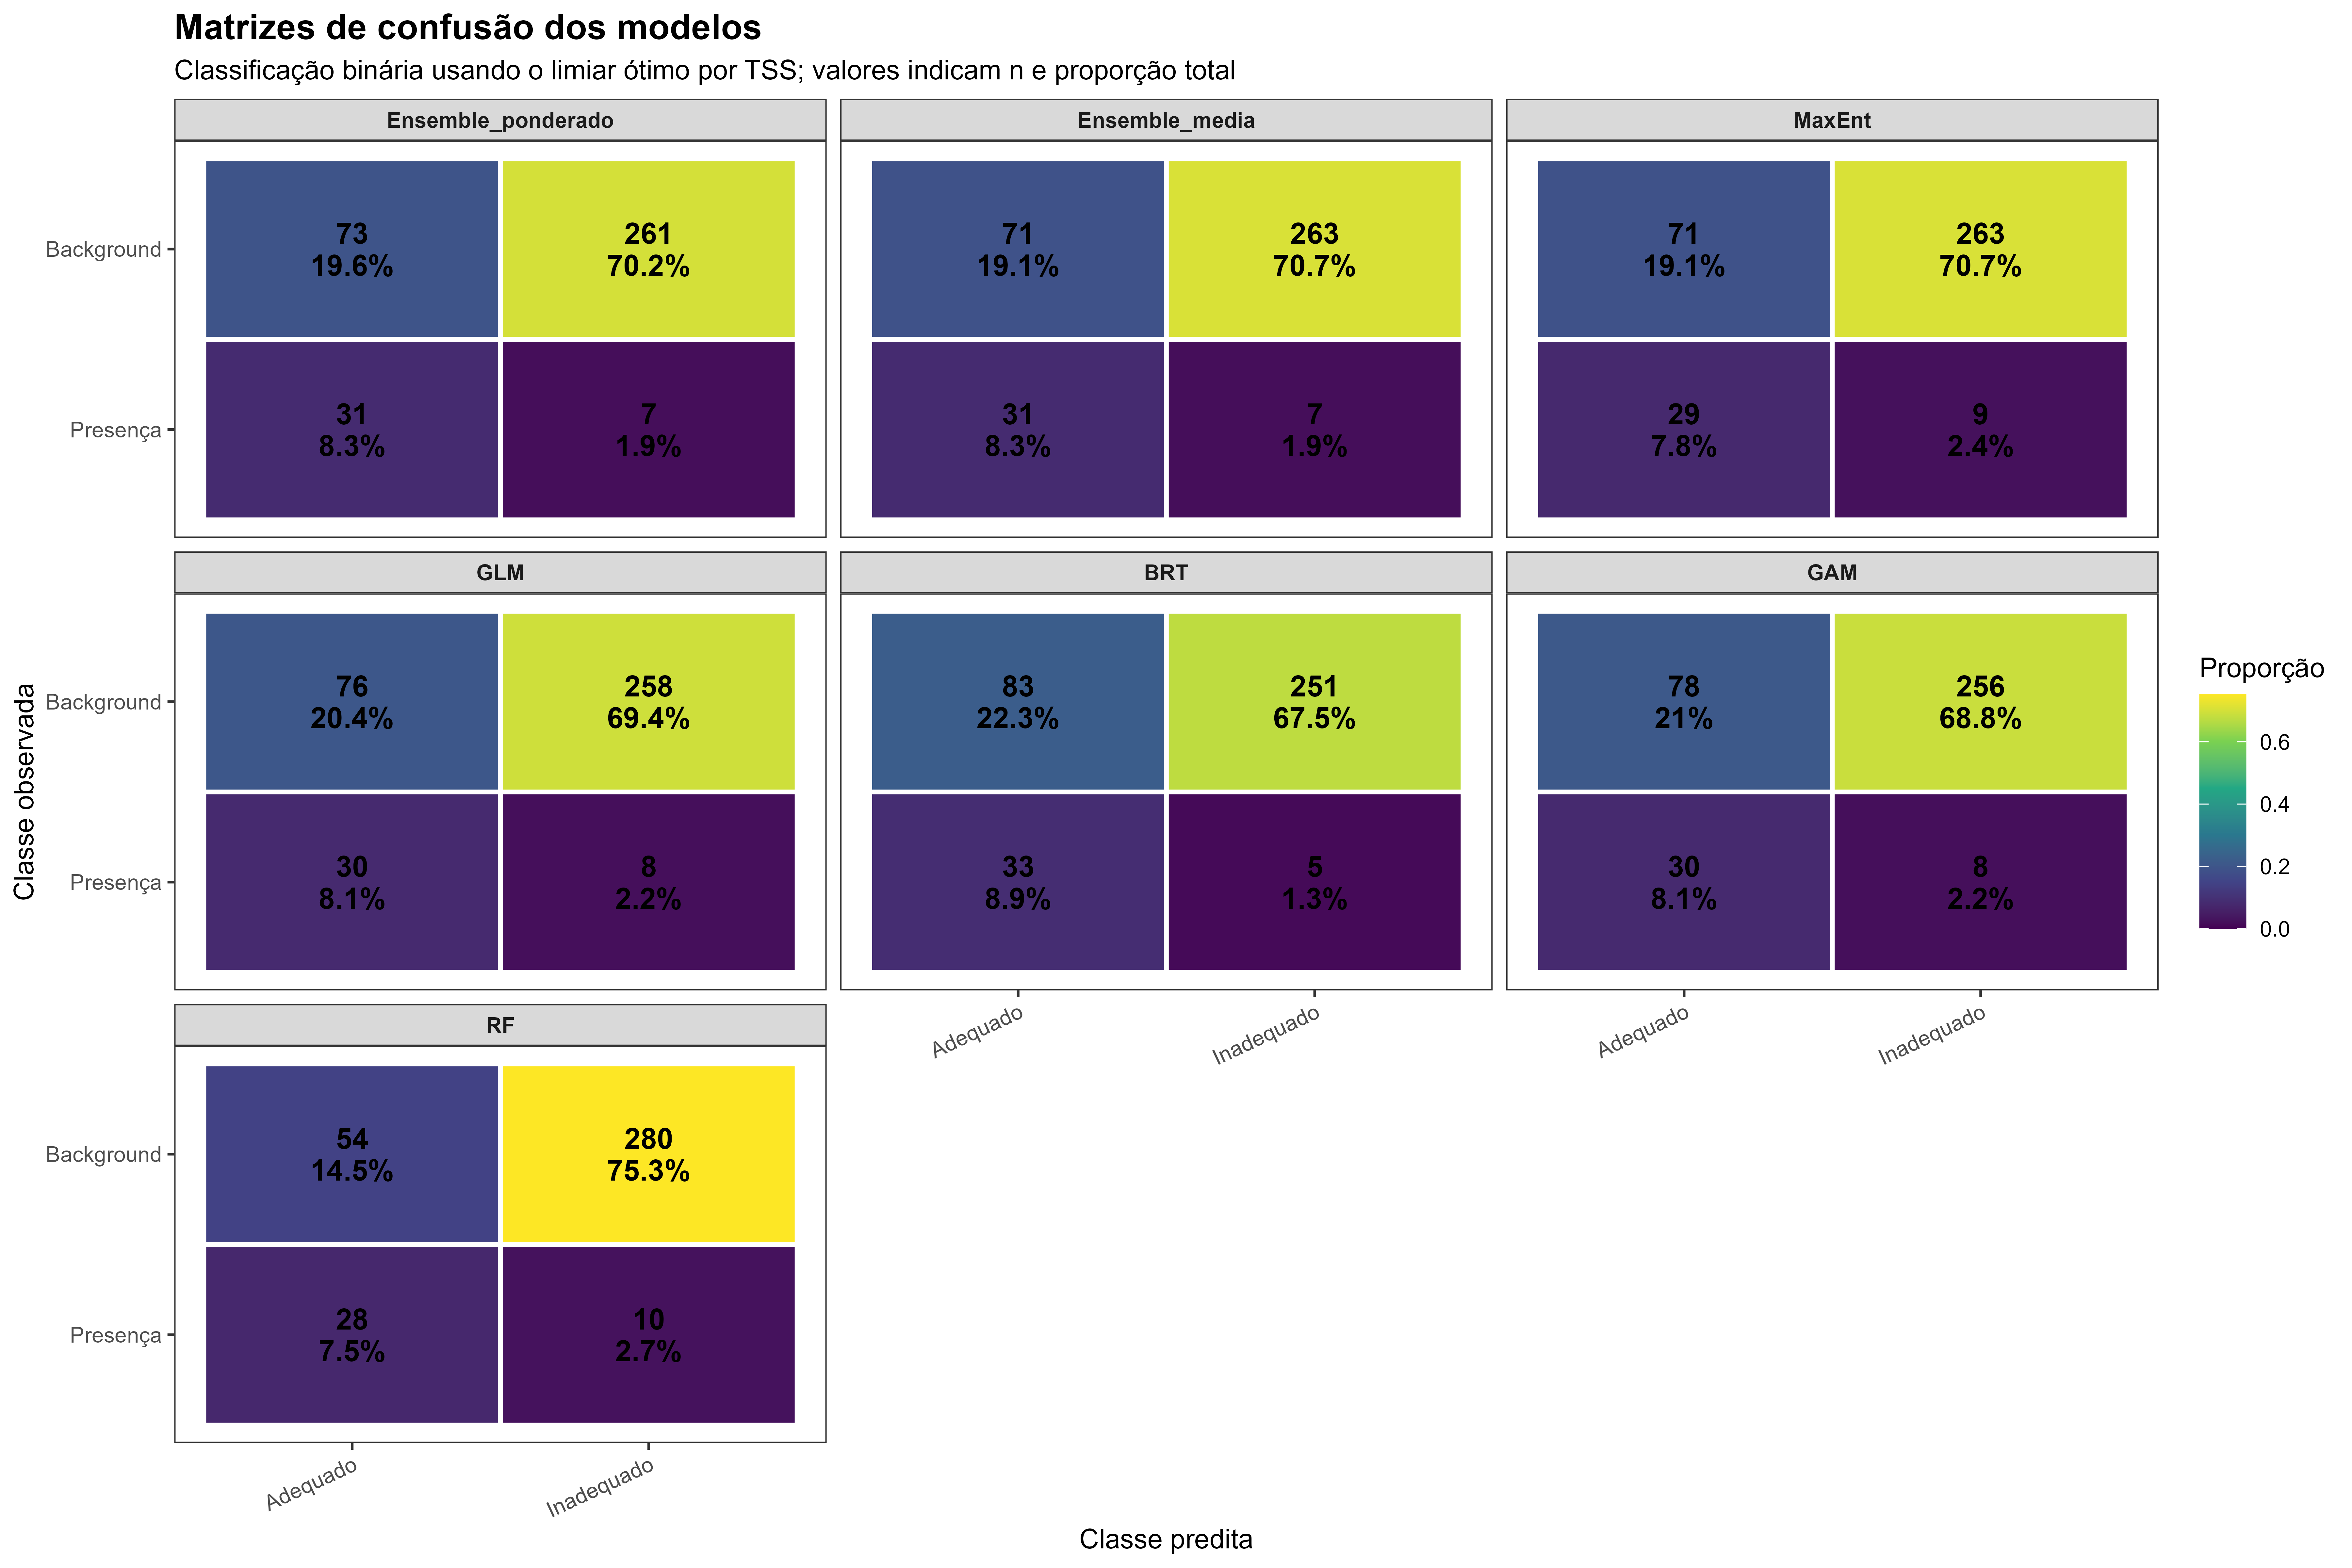
\includegraphics[width=0.95\textwidth]{figuras/unidade12/unidade12_matrizes_confusao.png}
\caption{Confusion matrices using TSS-selected thresholds.}\label{fig:unidade12_matrizes_confusao}
\end{figure}

\section{Binary Maps}
\rscriptfile{scripts/unidade12/06_mapas_binarios.R}
\begin{figure}[H]\centering
\includegraphics[width=0.98\textwidth]{figuras/unidade12/unidade12_mapas_binarios.png}
\caption{Binary suitability maps for \textit{Dinizia excelsa} using TSS-selected thresholds.}\label{fig:unidade12_mapas_binarios}
\end{figure}

\section{Comparative Synthesis}
\rscriptfile{scripts/unidade12/07_sintese_avaliacao.R}
\begin{figure}[H]\centering
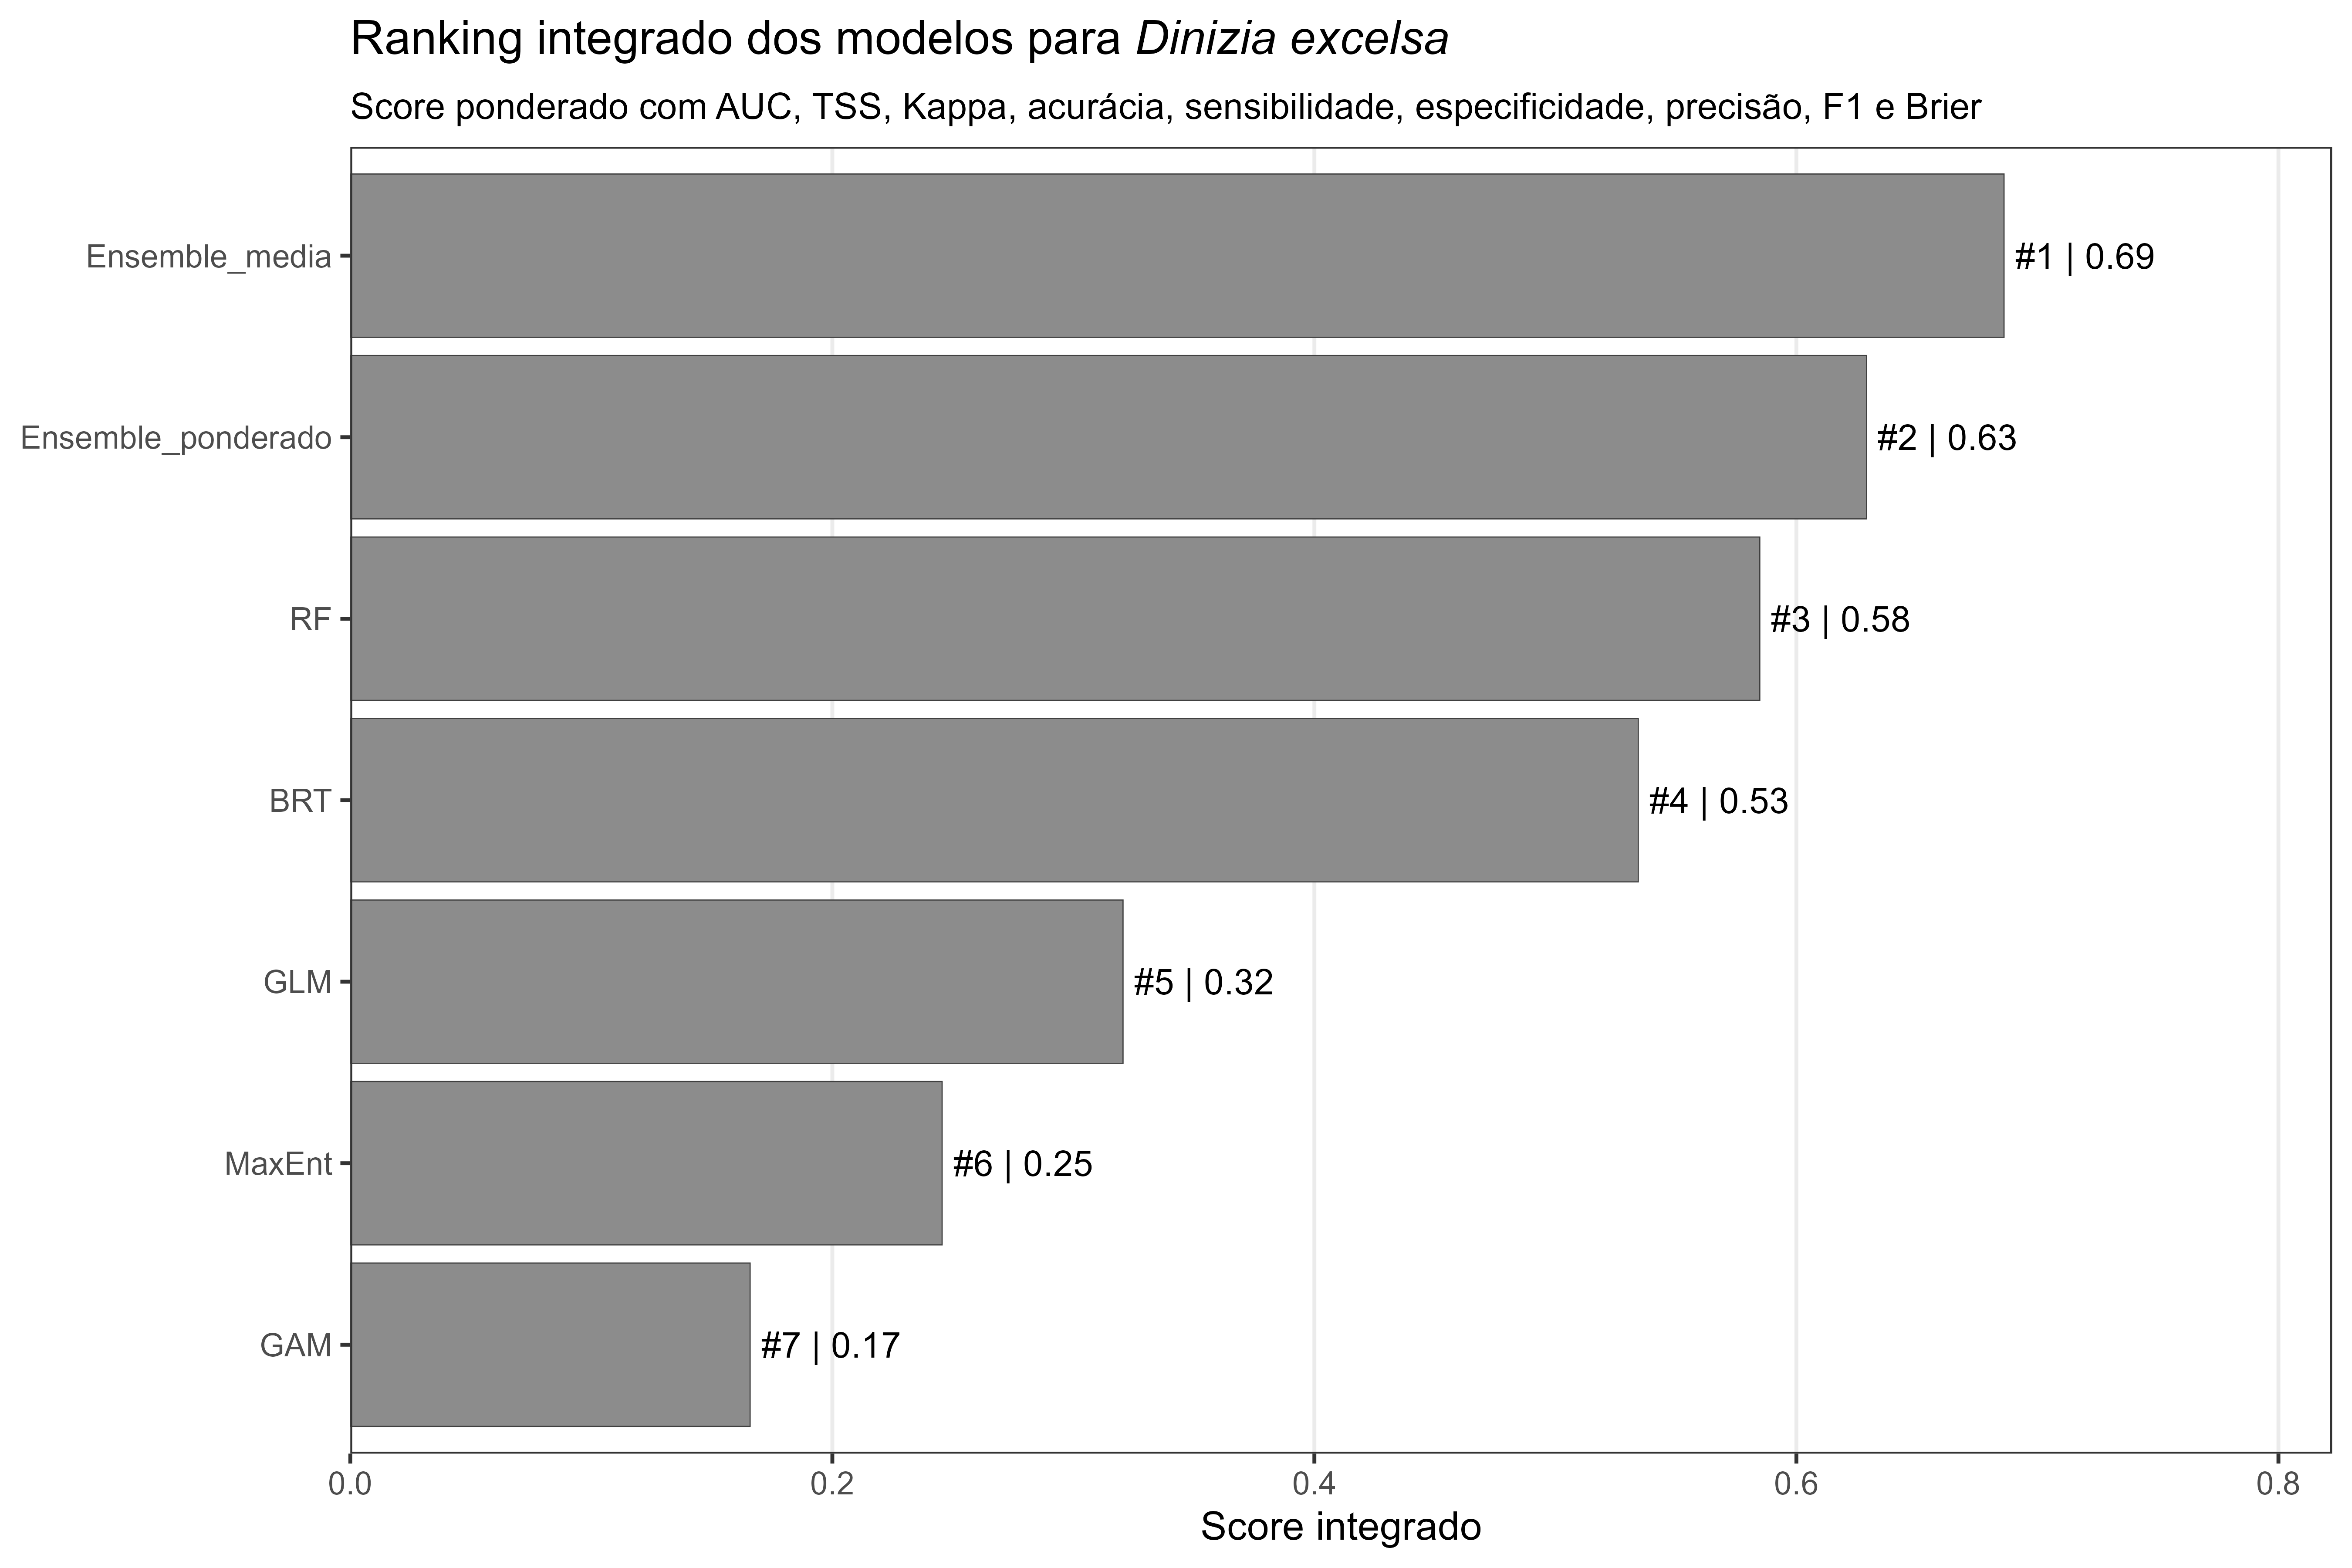
\includegraphics[width=0.95\textwidth]{figuras/unidade12/unidade12_ranking_modelos.png}
\caption{Comparative ranking using AUC, TSS, Kappa, sensitivity, specificity, and Boyce Index.}\label{fig:unidade12_ranking}
\end{figure}

\section{Complete Pipeline}
\rscriptfile{scripts/unidade12/08_pipeline_avaliacao.R}

\section{Chapter Summary}
Robust evaluation combines multiple metrics, independent validation, ecological
interpretation, response curves, uncertainty, and spatial plausibility.
\begin{conceito}[title={\faBook\quad Key message}]
No single metric validates an SDM. Robust evaluation combines continuous and
binary metrics, ecological interpretation, and spatial analysis of predictions.
\end{conceito}

\section{Review Exercises}
\subsection*{A. Concepts}
\begin{enumerate}
\item Explain the difference between AUC and TSS.
\item Why can AUC be problematic with presence--background data?
\item What do sensitivity and specificity mean?
\end{enumerate}
\subsection*{B. Interpretation}
\begin{enumerate}[resume]
\item Two models have the same AUC but different sensitivity. What are the consequences for identifying potentially suitable areas?
\item Performance decreases under spatial blocks. Interpret this without automatically rejecting the algorithm.
\item Explain the ecological meaning and one limitation of Boyce Index.
\end{enumerate}
\subsection*{C. Computation}
\begin{enumerate}[resume]
\item Recalculate metrics using identical folds and compare fold variation, not only means.
\item Construct spatial and environmental partitions; examine class balance in each fold.
\item Compare two thresholds and quantify changes in suitable area, omission, and commission.
\end{enumerate}
\subsection*{D. Critical Thinking}
\begin{enumerate}[resume]
\item Why should binary maps be interpreted cautiously?
\item How should validation differ between interpolation within Amazonia and projection to future climate?
\item Can a high-AUC presence--background model be called a well-calibrated occurrence-probability model? Justify.
\end{enumerate}

\subsection*{Mini-Project}
Select one \textit{Dinizia excelsa} algorithm. Compare random and spatial-block
evaluation while holding data, predictors, and metrics constant. Present the
fold map, training--test distance distribution, fold-specific metrics, and a
recommendation for interpolation and transfer.

\chapter[Future climate projections]{Future Climate Projections in Species Distribution Modeling}

\begin{objetivos}
By the end of this chapter, readers should be able to explain how species distribution models are projected under future climate conditions; recognize the principal CMIP6 Shared Socioeconomic Pathways (SSPs); harmonize future and baseline environmental predictors; project fitted models for \textit{Dinizia excelsa}; map future environmental suitability; quantify changes in suitability; identify areas of potential stability, loss, and gain; and discuss uncertainty arising from scenarios, global climate models, time horizons, and SDM algorithms.
\end{objetivos}

\section{Introduction}

Future climate projections are used to investigate how the potential environmental suitability of a species may change under alternative climate trajectories. In SDM, models calibrated with baseline occurrence and environmental data are transferred to future predictor layers derived from global climate models (GCMs), future periods, and socioeconomic pathways \parencite{guisan2017habitat,ipcc2021,araujo2006climate,thuiller2005climate}.

This chapter develops a reproducible workflow for \textit{Dinizia excelsa} using the predictors selected in previous chapters, the accessible area \(M\), the fitted algorithms, and the baseline ensemble. Projections are organized for SSP1--2.6, SSP2--4.5, SSP3--7.0, and SSP5--8.5. In filenames and R objects, these pathways may appear in the compact forms SSP126, SSP245, SSP370, and SSP585.

\begin{conceito}[title={\faBook\quad Future climate projection}]
A future SDM projection applies a model calibrated under baseline conditions to environmental predictors representing a specified future climate. Its output is not a deterministic forecast of species presence. It is a conditional estimate of environmental suitability, given the fitted model, predictor set, climate model, pathway, time horizon, and assumptions about transferability.
\end{conceito}

\section{CMIP6 and Shared Socioeconomic Pathways}

The Coupled Model Intercomparison Project Phase 6 (CMIP6) coordinates climate simulations produced by multiple modeling centers. Shared Socioeconomic Pathways describe alternative socioeconomic development trajectories. When paired with climate-policy assumptions, they are associated with approximate radiative-forcing levels by 2100. The final number in each scenario label indicates that forcing level in W\,m\(^{-2}\), rather than a probability assigned to the scenario.

\begin{itemize}
\item SSP1--2.6: a sustainability-oriented pathway associated with low forcing and strong mitigation;
\item SSP2--4.5: an intermediate pathway associated with moderate forcing;
\item SSP3--7.0: a regionally fragmented pathway associated with high forcing;
\item SSP5--8.5: a fossil-fuel-intensive pathway associated with very high forcing.
\end{itemize}

\begin{atencao}[title={\faExclamationTriangle\quad A scenario is not a unique forecast}]
Each SSP-based projection represents a conditional future, not a certain outcome. Results should therefore be compared across pathways, GCMs, and time horizons. Treating one GCM--SSP combination as ``the future'' understates scenario and climate-model uncertainty.
\end{atencao}

\section{Compatibility between baseline and future predictors}

Future layers must represent the same predictor definitions and units used for calibration. They must also have compatible names, spatial resolution, coordinate reference system, extent, cell origin, and mask. Apparent compatibility based only on filenames is insufficient: temporal summaries, variable definitions, unit conversions, and downscaling products must also be checked. A mismatch can cause a computational error or, more seriously, produce a numerically valid but scientifically invalid projection.

\rscriptfile{scripts/unidade13/01_estrutura_pastas.R}

\rscriptfile{scripts/unidade13/02_preparar_variaveis_futuras.R}

\section{Projecting individual models}

The GLM, GAM, Random Forest, BRT, and Maxent models are projected to the future scenarios using the same predictor set employed during calibration. The analysis mask defines the reported projection domain; it should not be interpreted as proof that the species will be able to disperse to every newly suitable cell. Assumptions about dispersal, land-use continuity, biotic interactions, and demographic persistence remain external to a climate-only projection.

\rscriptfile{scripts/unidade13/03_projetar_modelos_futuros.R}

\begin{figure}[H]
\centering
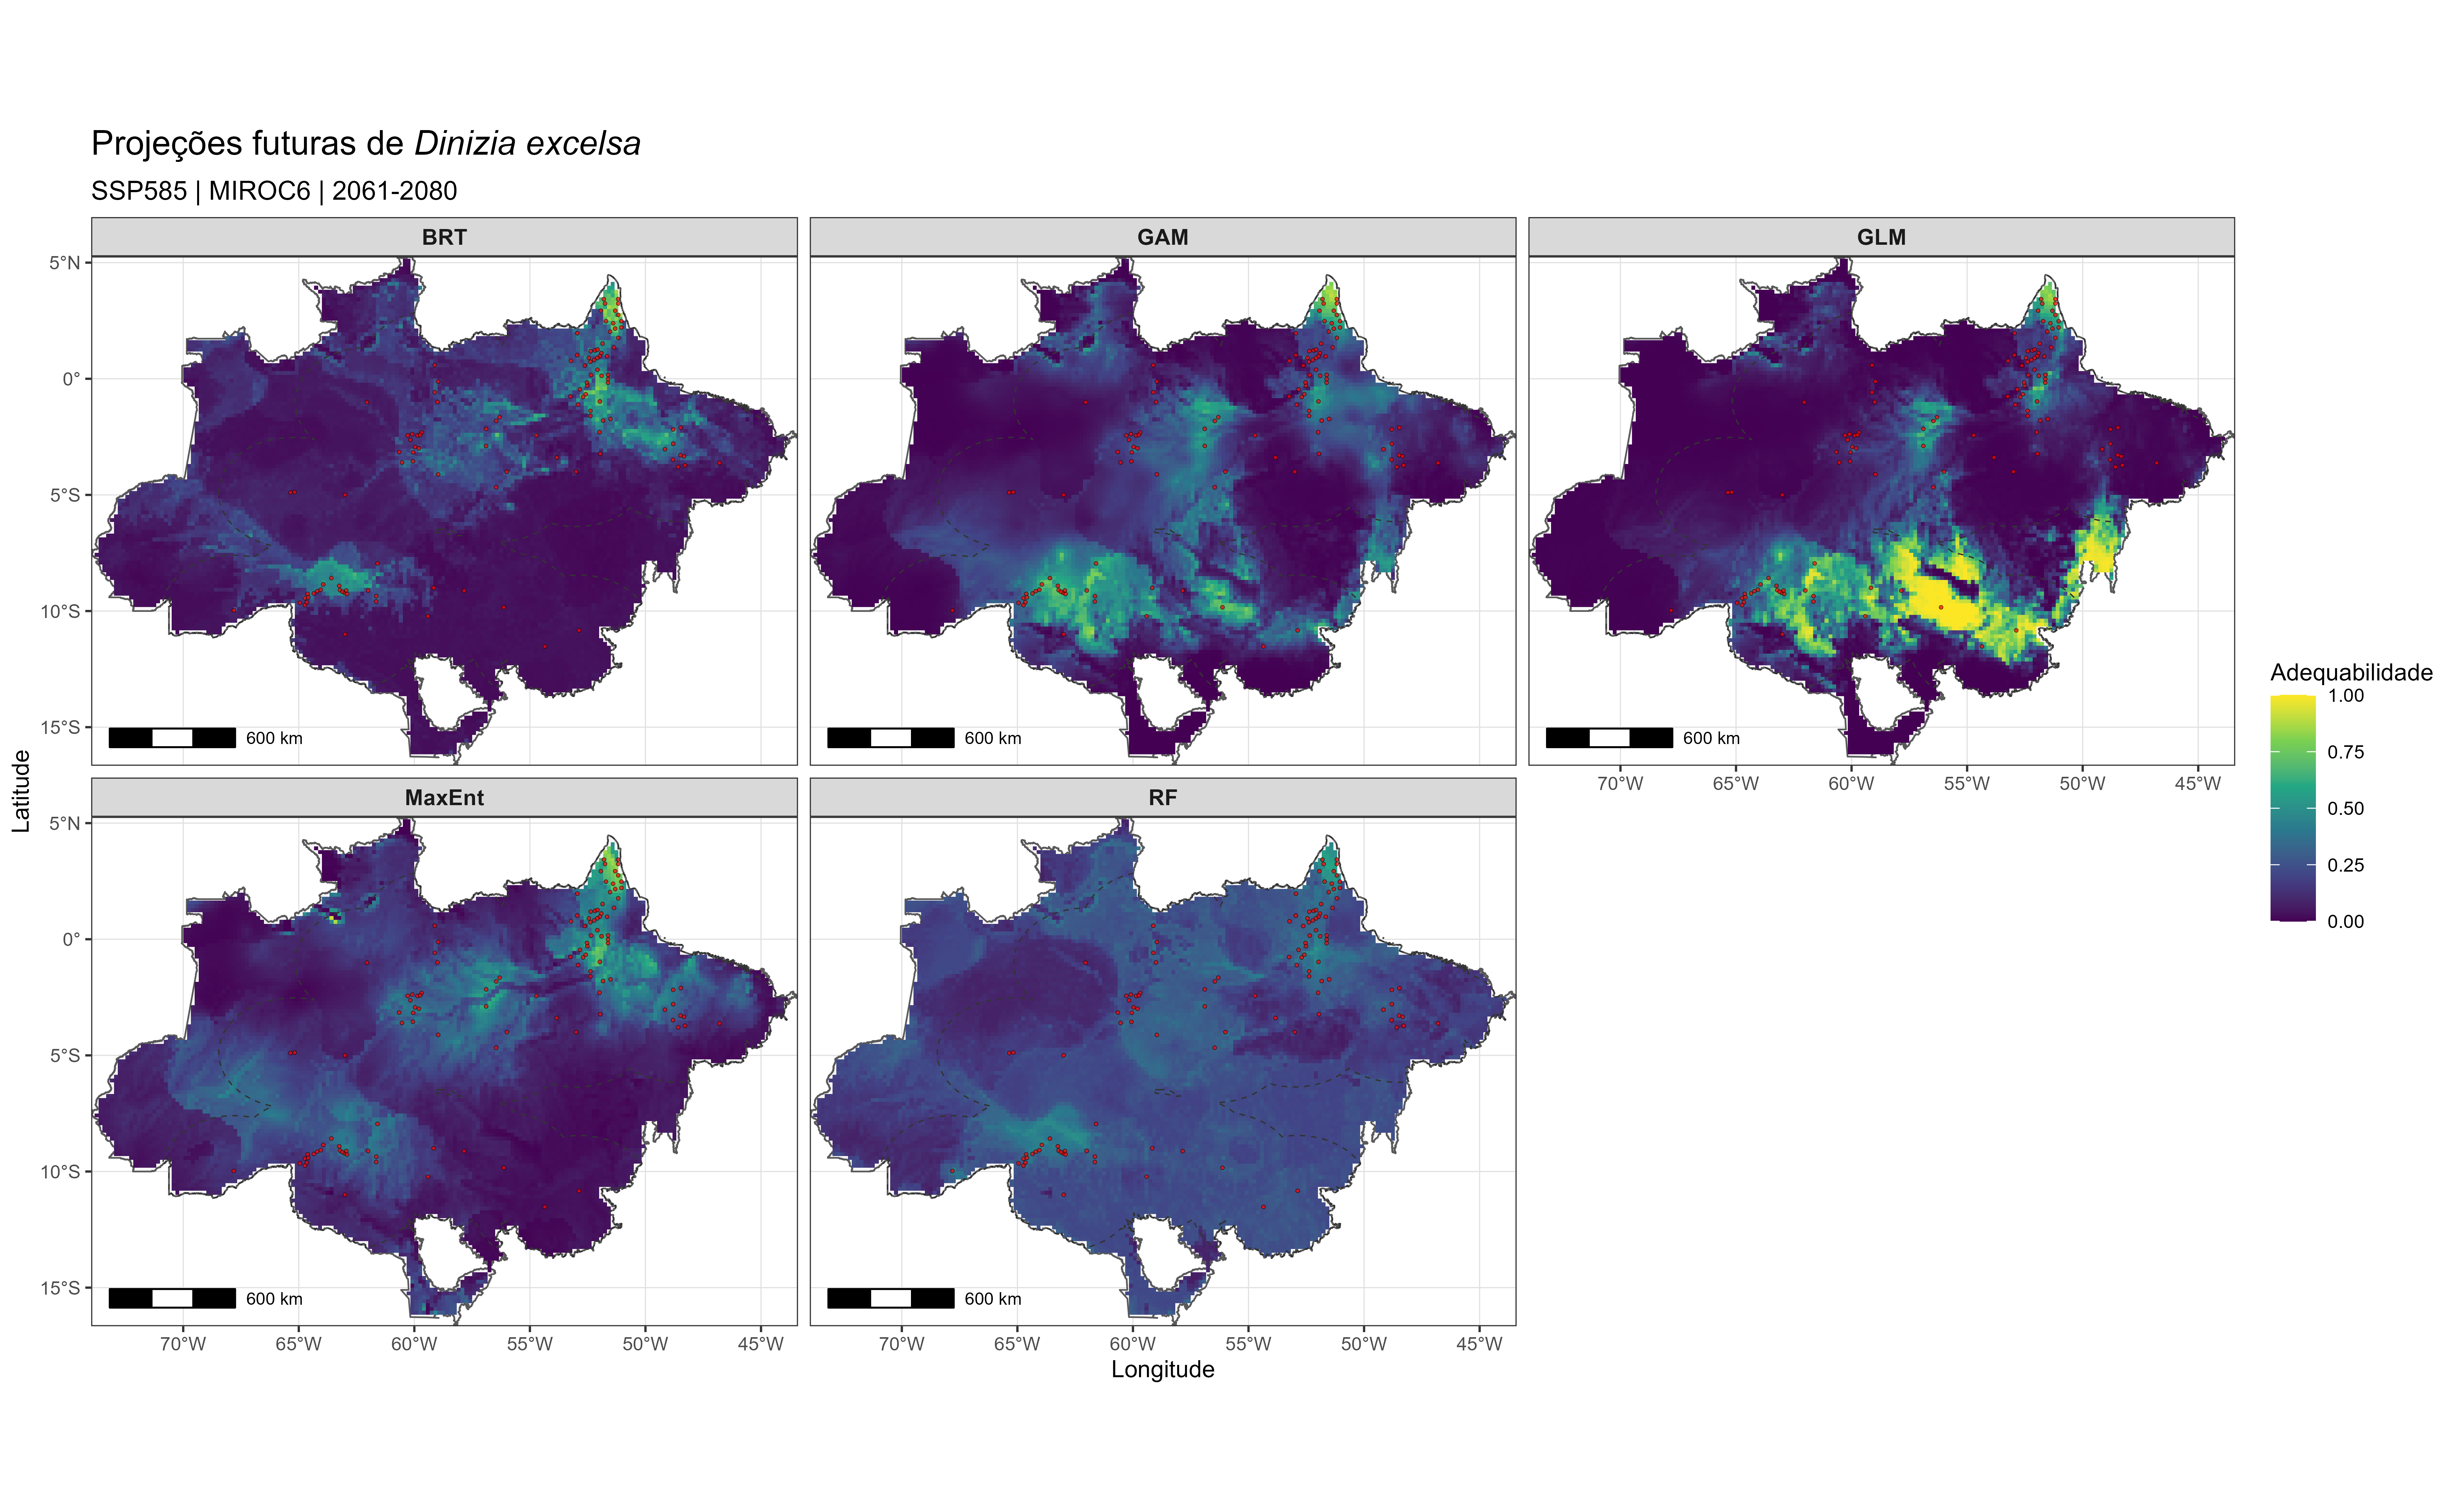
\includegraphics[width=0.98\textwidth]{figuras/unidade13/unidade13_modelos_futuros_ssp585.png}
\caption{Future projections from the individual models for \textit{Dinizia excelsa} under SSP5--8.5. Differences among panels represent algorithmic uncertainty conditional on the same climate scenario.}
\label{fig:unidade13_modelos_futuros}
\end{figure}

\section{Future ensemble projections}

Individual projections are combined into an ensemble for each scenario. An ensemble reduces reliance on a single algorithm and summarizes central tendencies across models, but it does not remove shared biases in occurrences, predictors, sampling, calibration extent, or climate inputs. Model weights and inclusion rules must therefore be fixed transparently and applied consistently across baseline and future conditions.

\rscriptfile{scripts/unidade13/04_ensemble_futuro.R}

\begin{figure}[H]
\centering
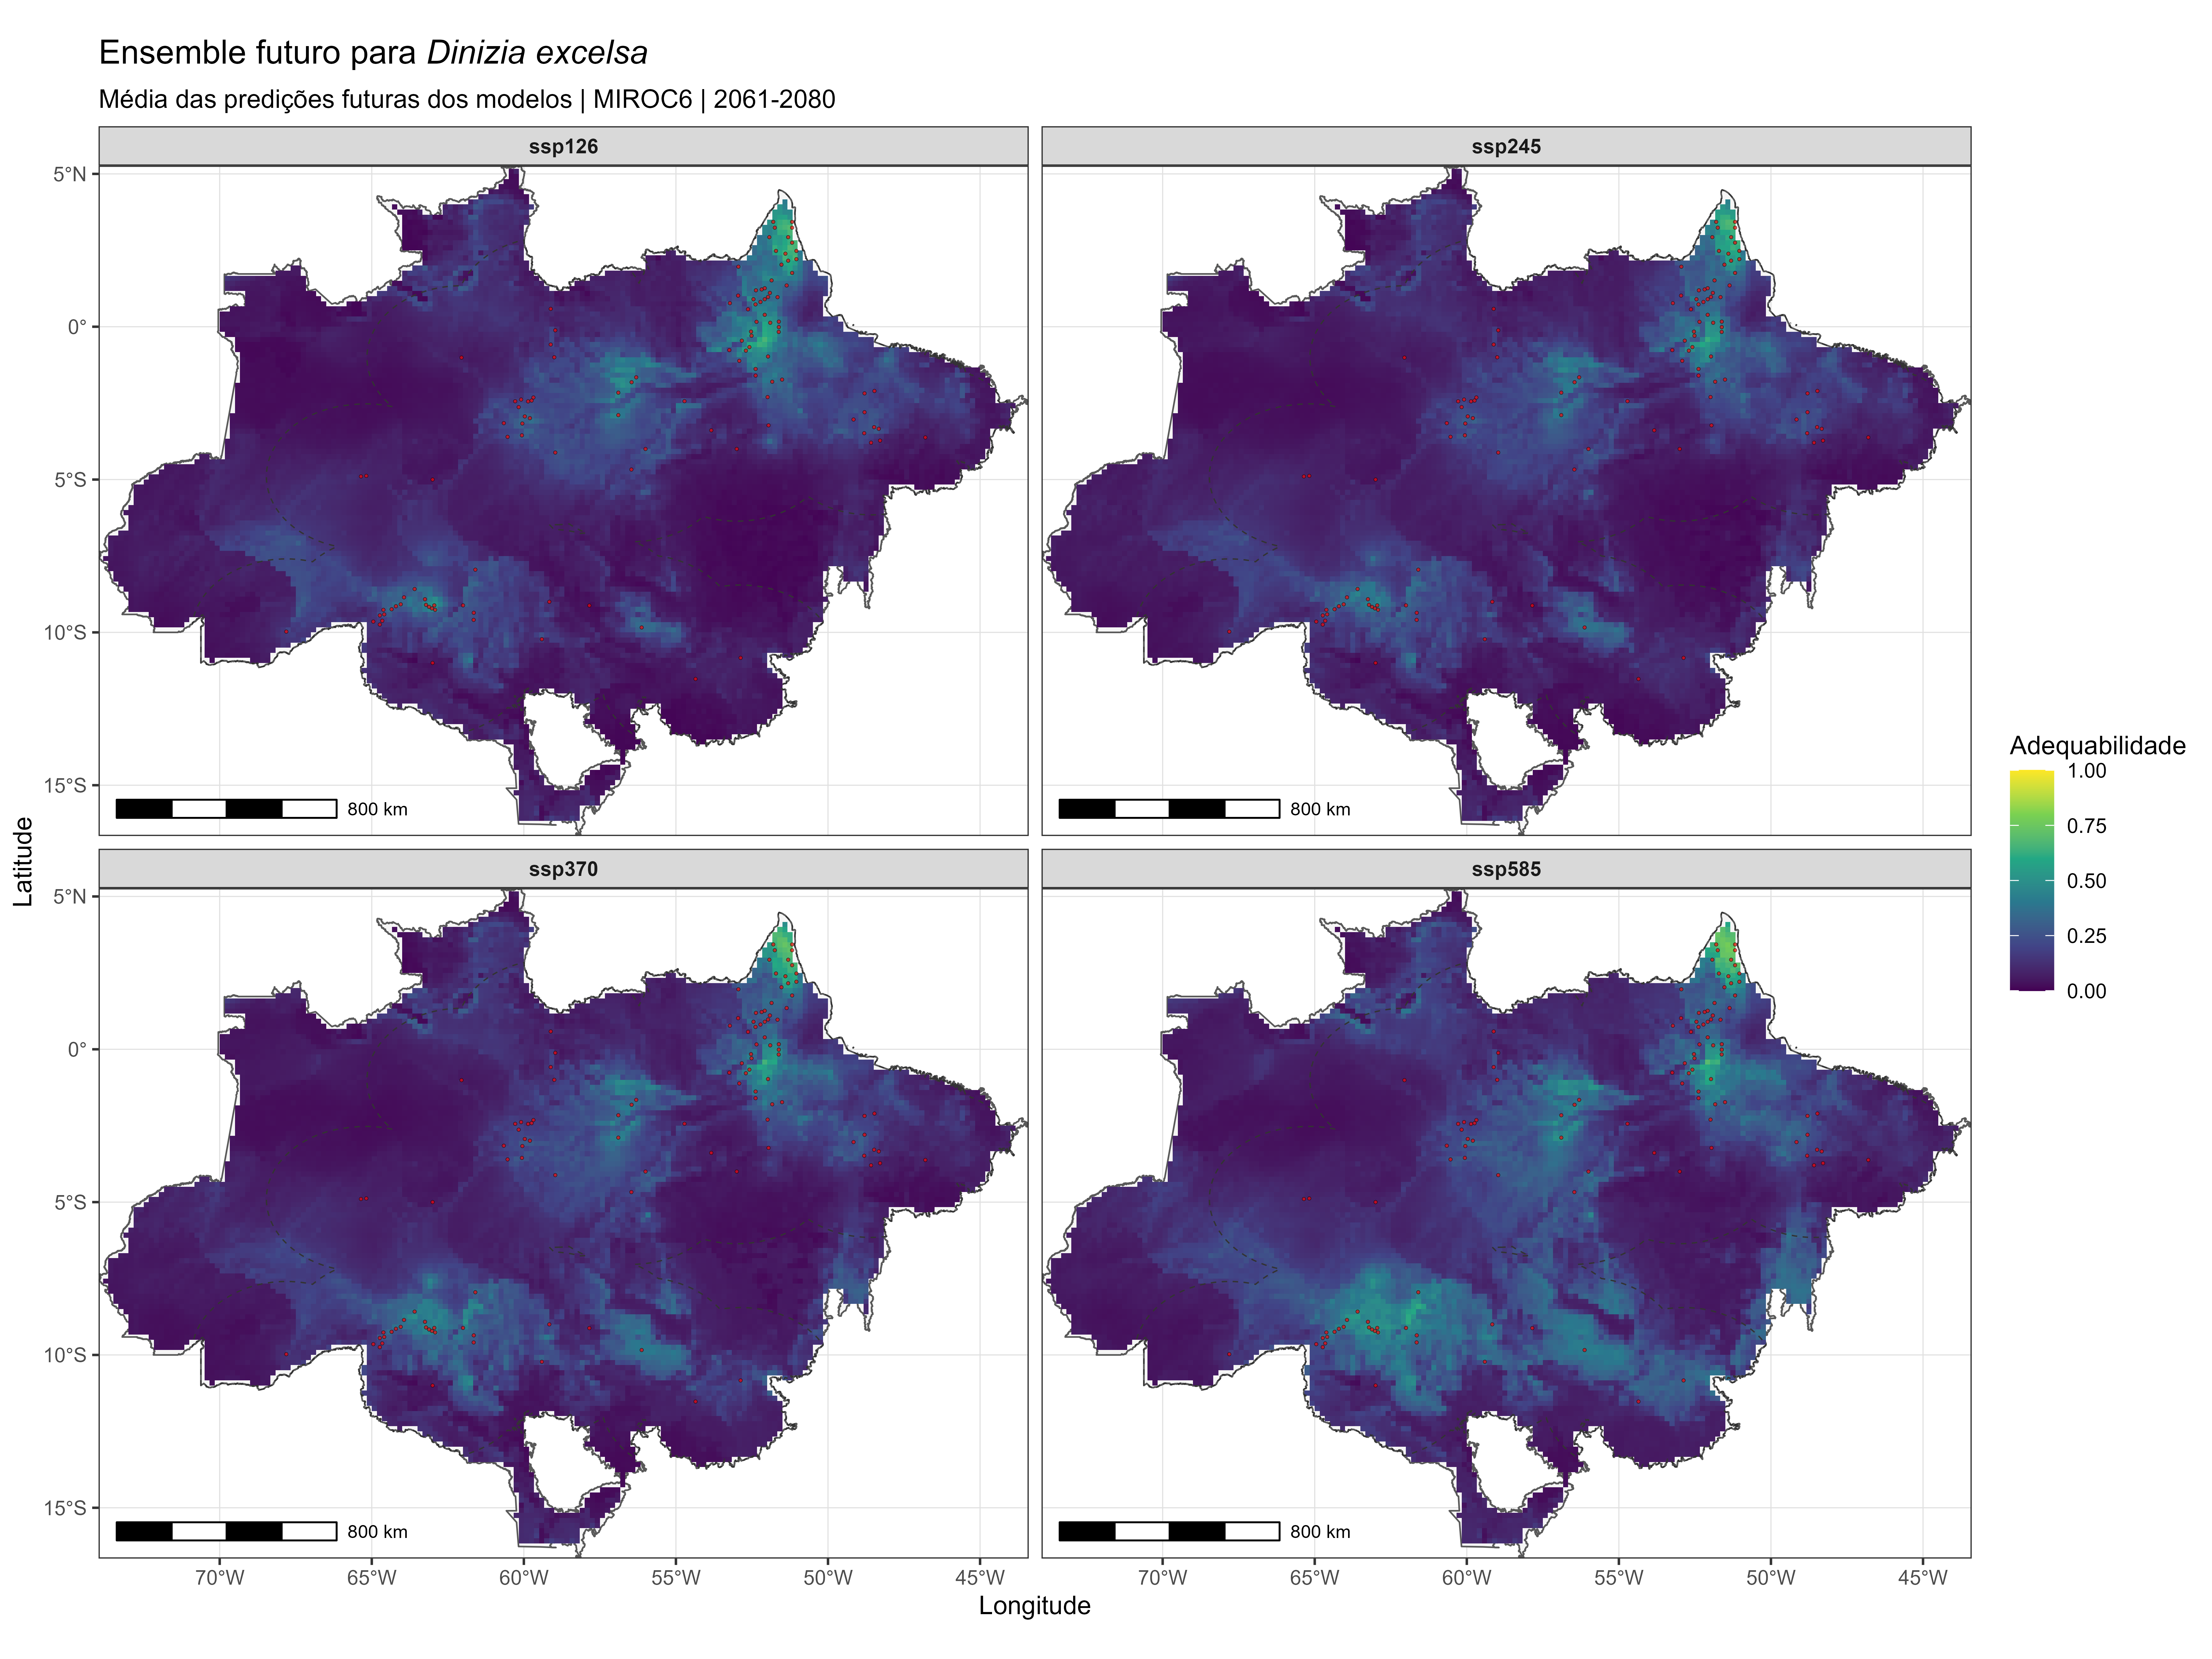
\includegraphics[width=0.96\textwidth]{figuras/unidade13/unidade13_ensemble_futuro_cenarios.png}
\caption{Ensemble projections of future environmental suitability for \textit{Dinizia excelsa} under alternative SSPs.}
\label{fig:unidade13_ensemble_futuro}
\end{figure}

\section{Change in suitability}

Suitability change is calculated as the cellwise difference between future and baseline predictions:

\begin{equationbox}
\[
\Delta S = S_{\mathrm{future}} - S_{\mathrm{baseline}}.
\]
\end{equationbox}

Here, \(S_{\mathrm{future}}\) is the projected suitability for a specified GCM, pathway, and period, and \(S_{\mathrm{baseline}}\) is the estimate for the baseline period. Positive values indicate a relative increase and negative values a relative decrease on the model's output scale. Differences are comparable only when baseline and future predictions were produced with the same fitted model, transformation, and scaling.

\rscriptfile{scripts/unidade13/05_mudanca_adequabilidade.R}

\begin{figure}[H]
\centering
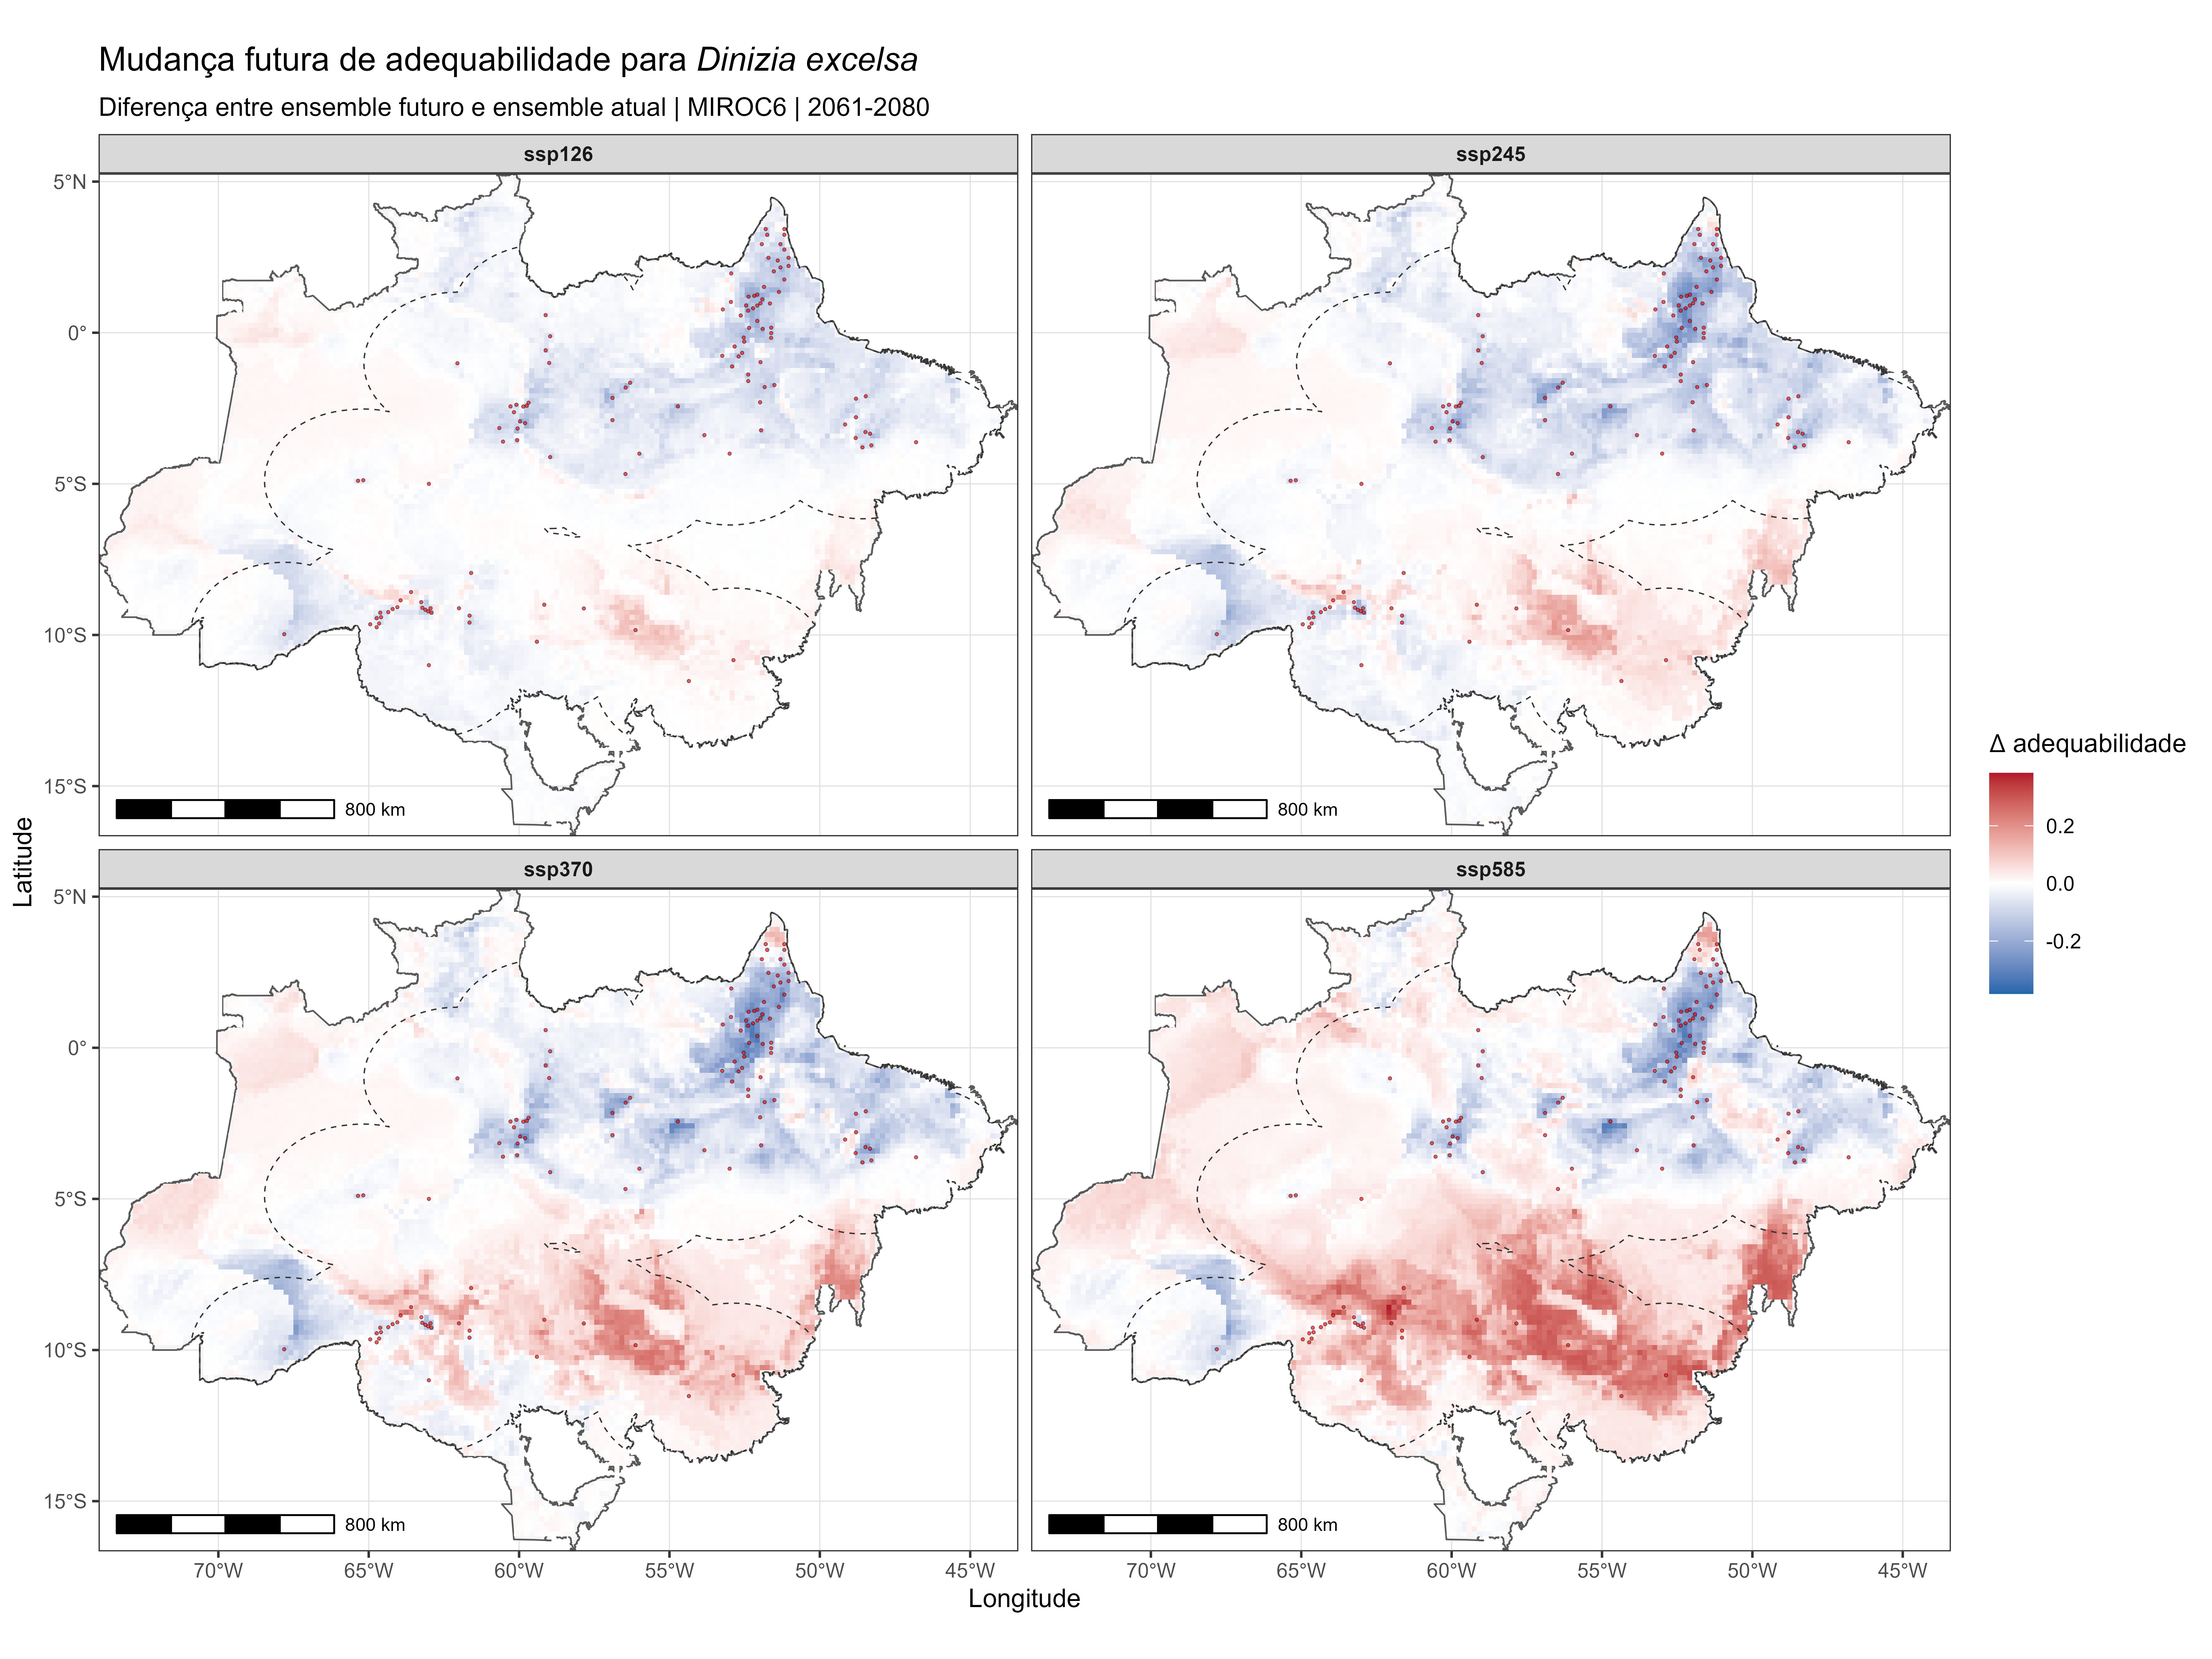
\includegraphics[width=0.96\textwidth]{figuras/unidade13/unidade13_mudanca_adequabilidade.png}
\caption{Projected change in environmental suitability relative to baseline conditions for \textit{Dinizia excelsa}.}
\label{fig:unidade13_mudanca}
\end{figure}

\section{Potential stability, loss, and gain}

Comparing thresholded baseline and future maps classifies cells as stable suitable, potential loss, potential gain, or persistently unsuitable. Because these categories depend on the selected threshold, their areal estimates should be accompanied by the threshold rule and, where feasible, a sensitivity analysis. A potential gain is not equivalent to colonization: accessibility, dispersal, establishment, habitat condition, and biotic constraints must also be considered.

\rscriptfile{scripts/unidade13/06_estabilidade_perda_ganho.R}

\begin{figure}[H]
\centering
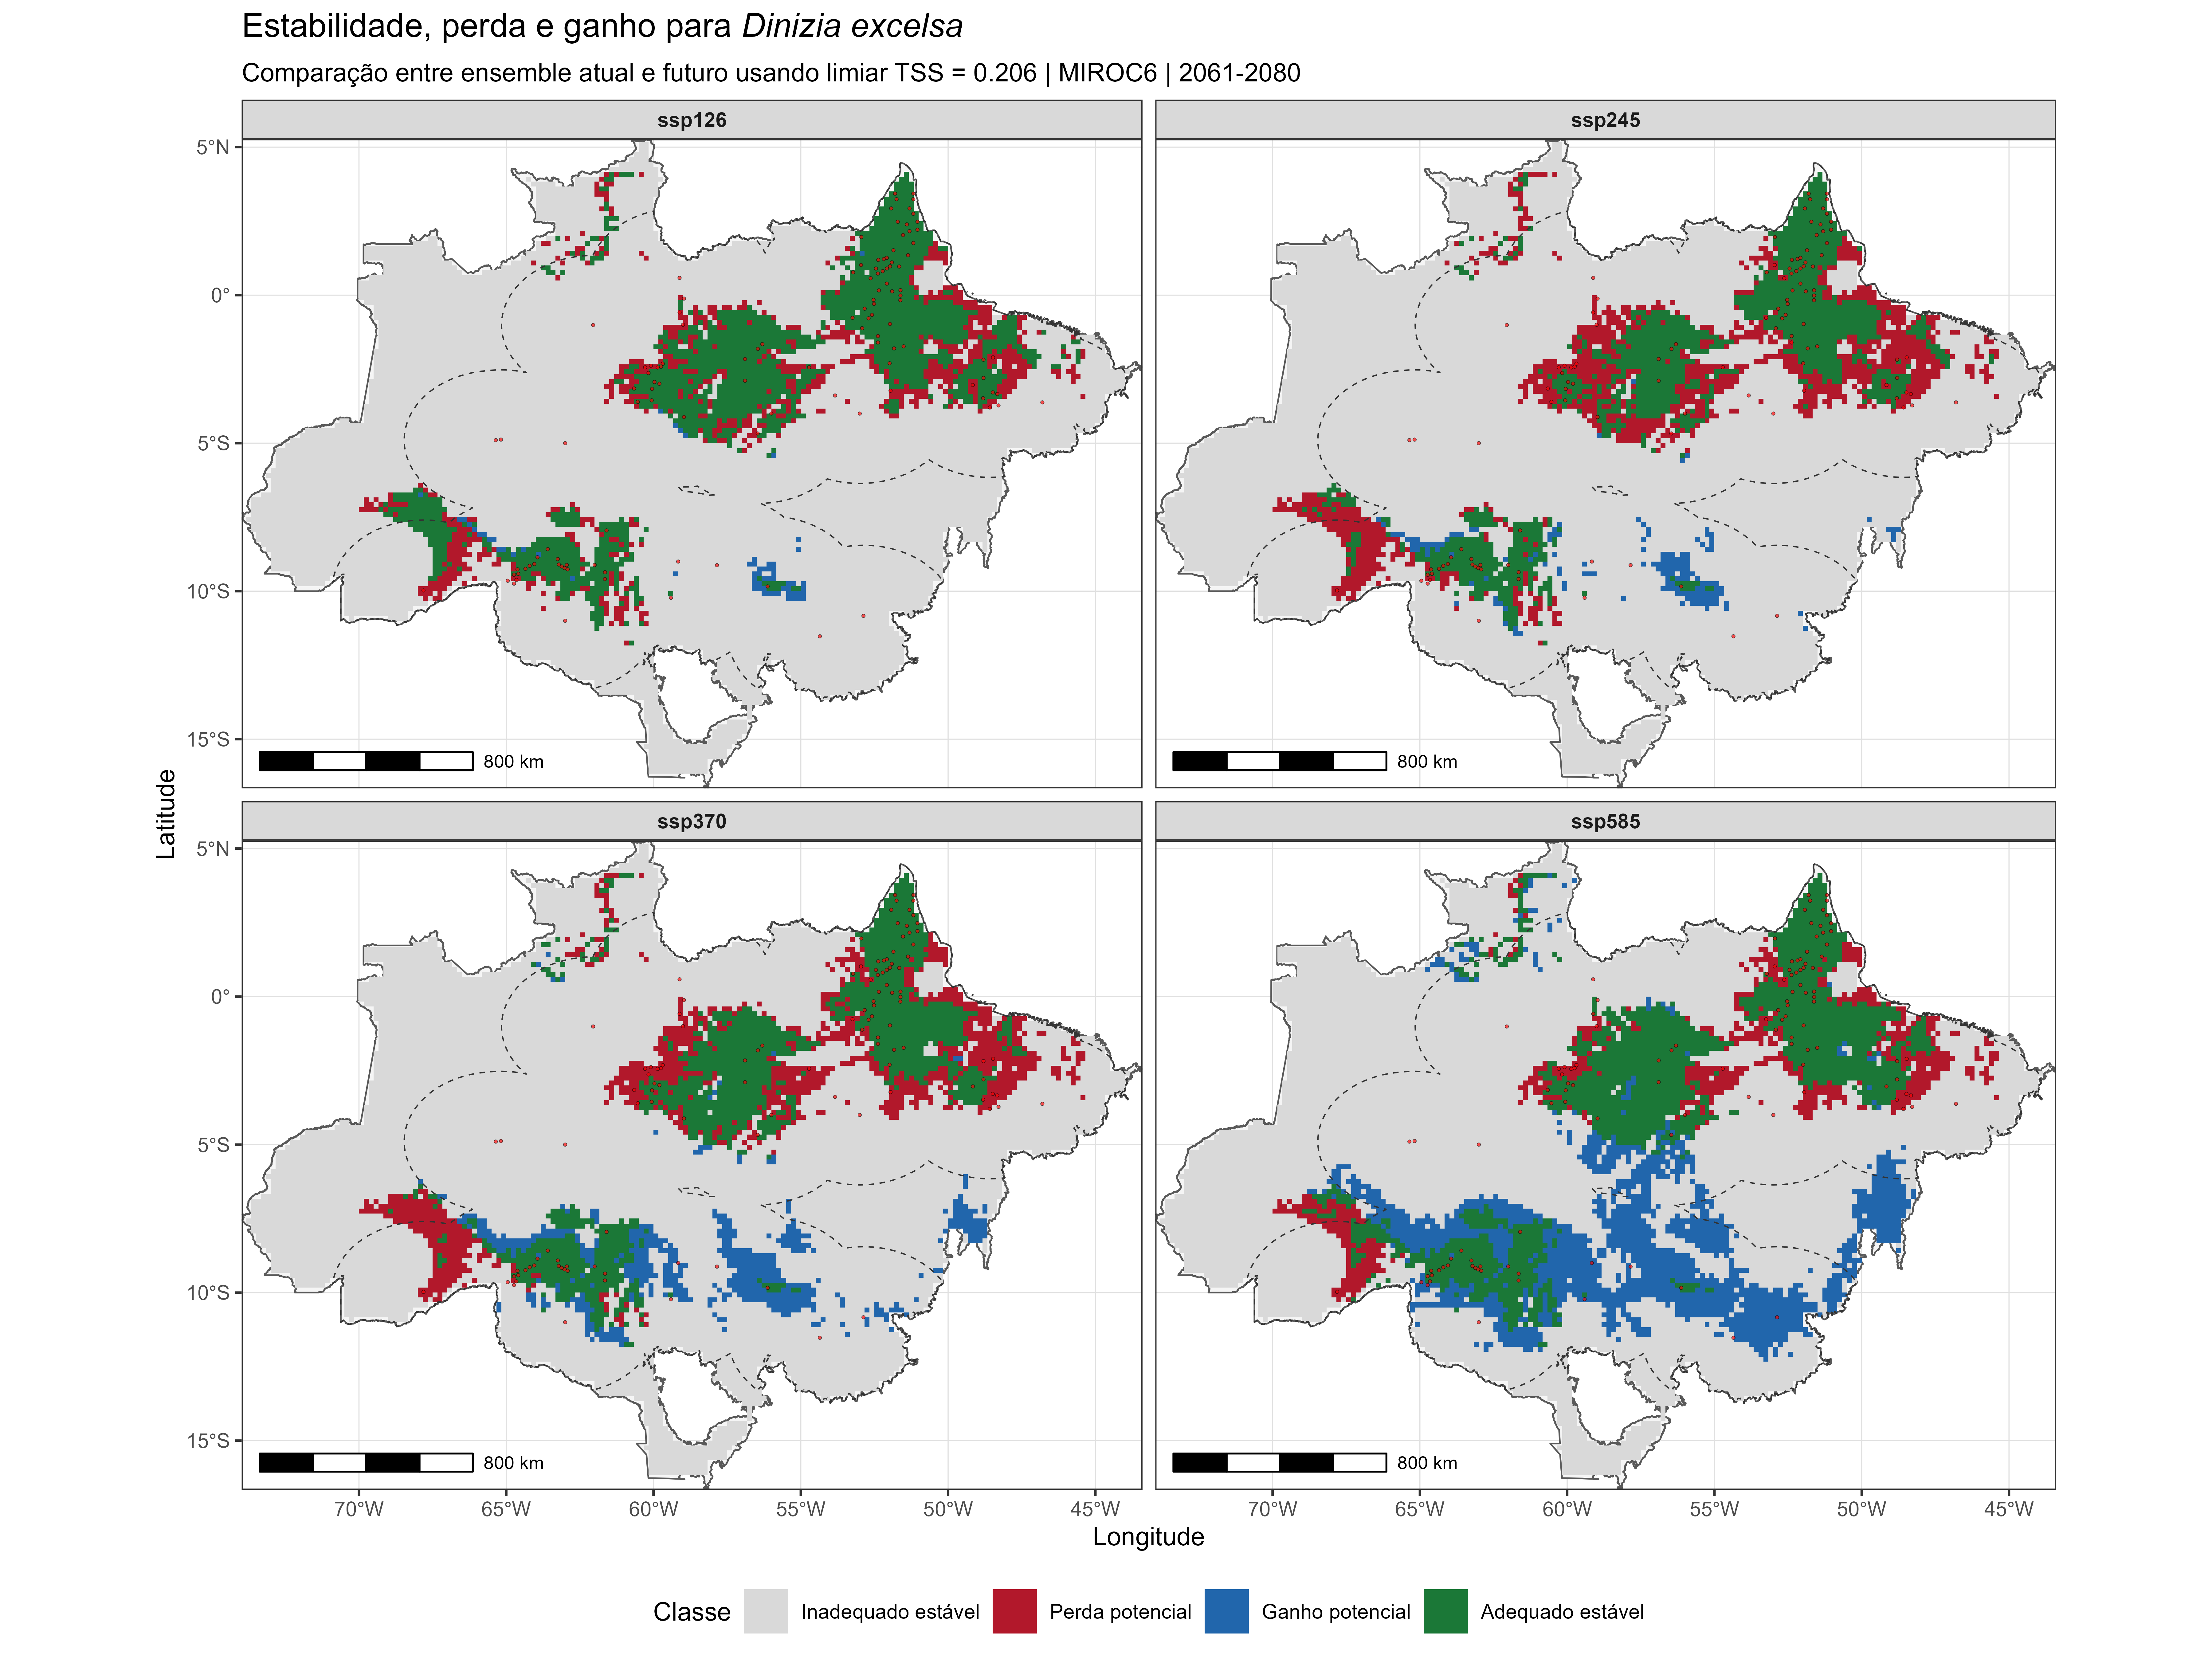
\includegraphics[width=0.96\textwidth]{figuras/unidade13/unidade13_estabilidade_perda_ganho.png}
\caption{Areas of potential stability, loss, and gain in environmental suitability for \textit{Dinizia excelsa} under future scenarios.}
\label{fig:unidade13_estabilidade}
\end{figure}

\section{Tabular synthesis across scenarios}

\rscriptfile{scripts/unidade13/07_sintese_cenarios_futuros.R}

\begin{figure}[H]
\centering
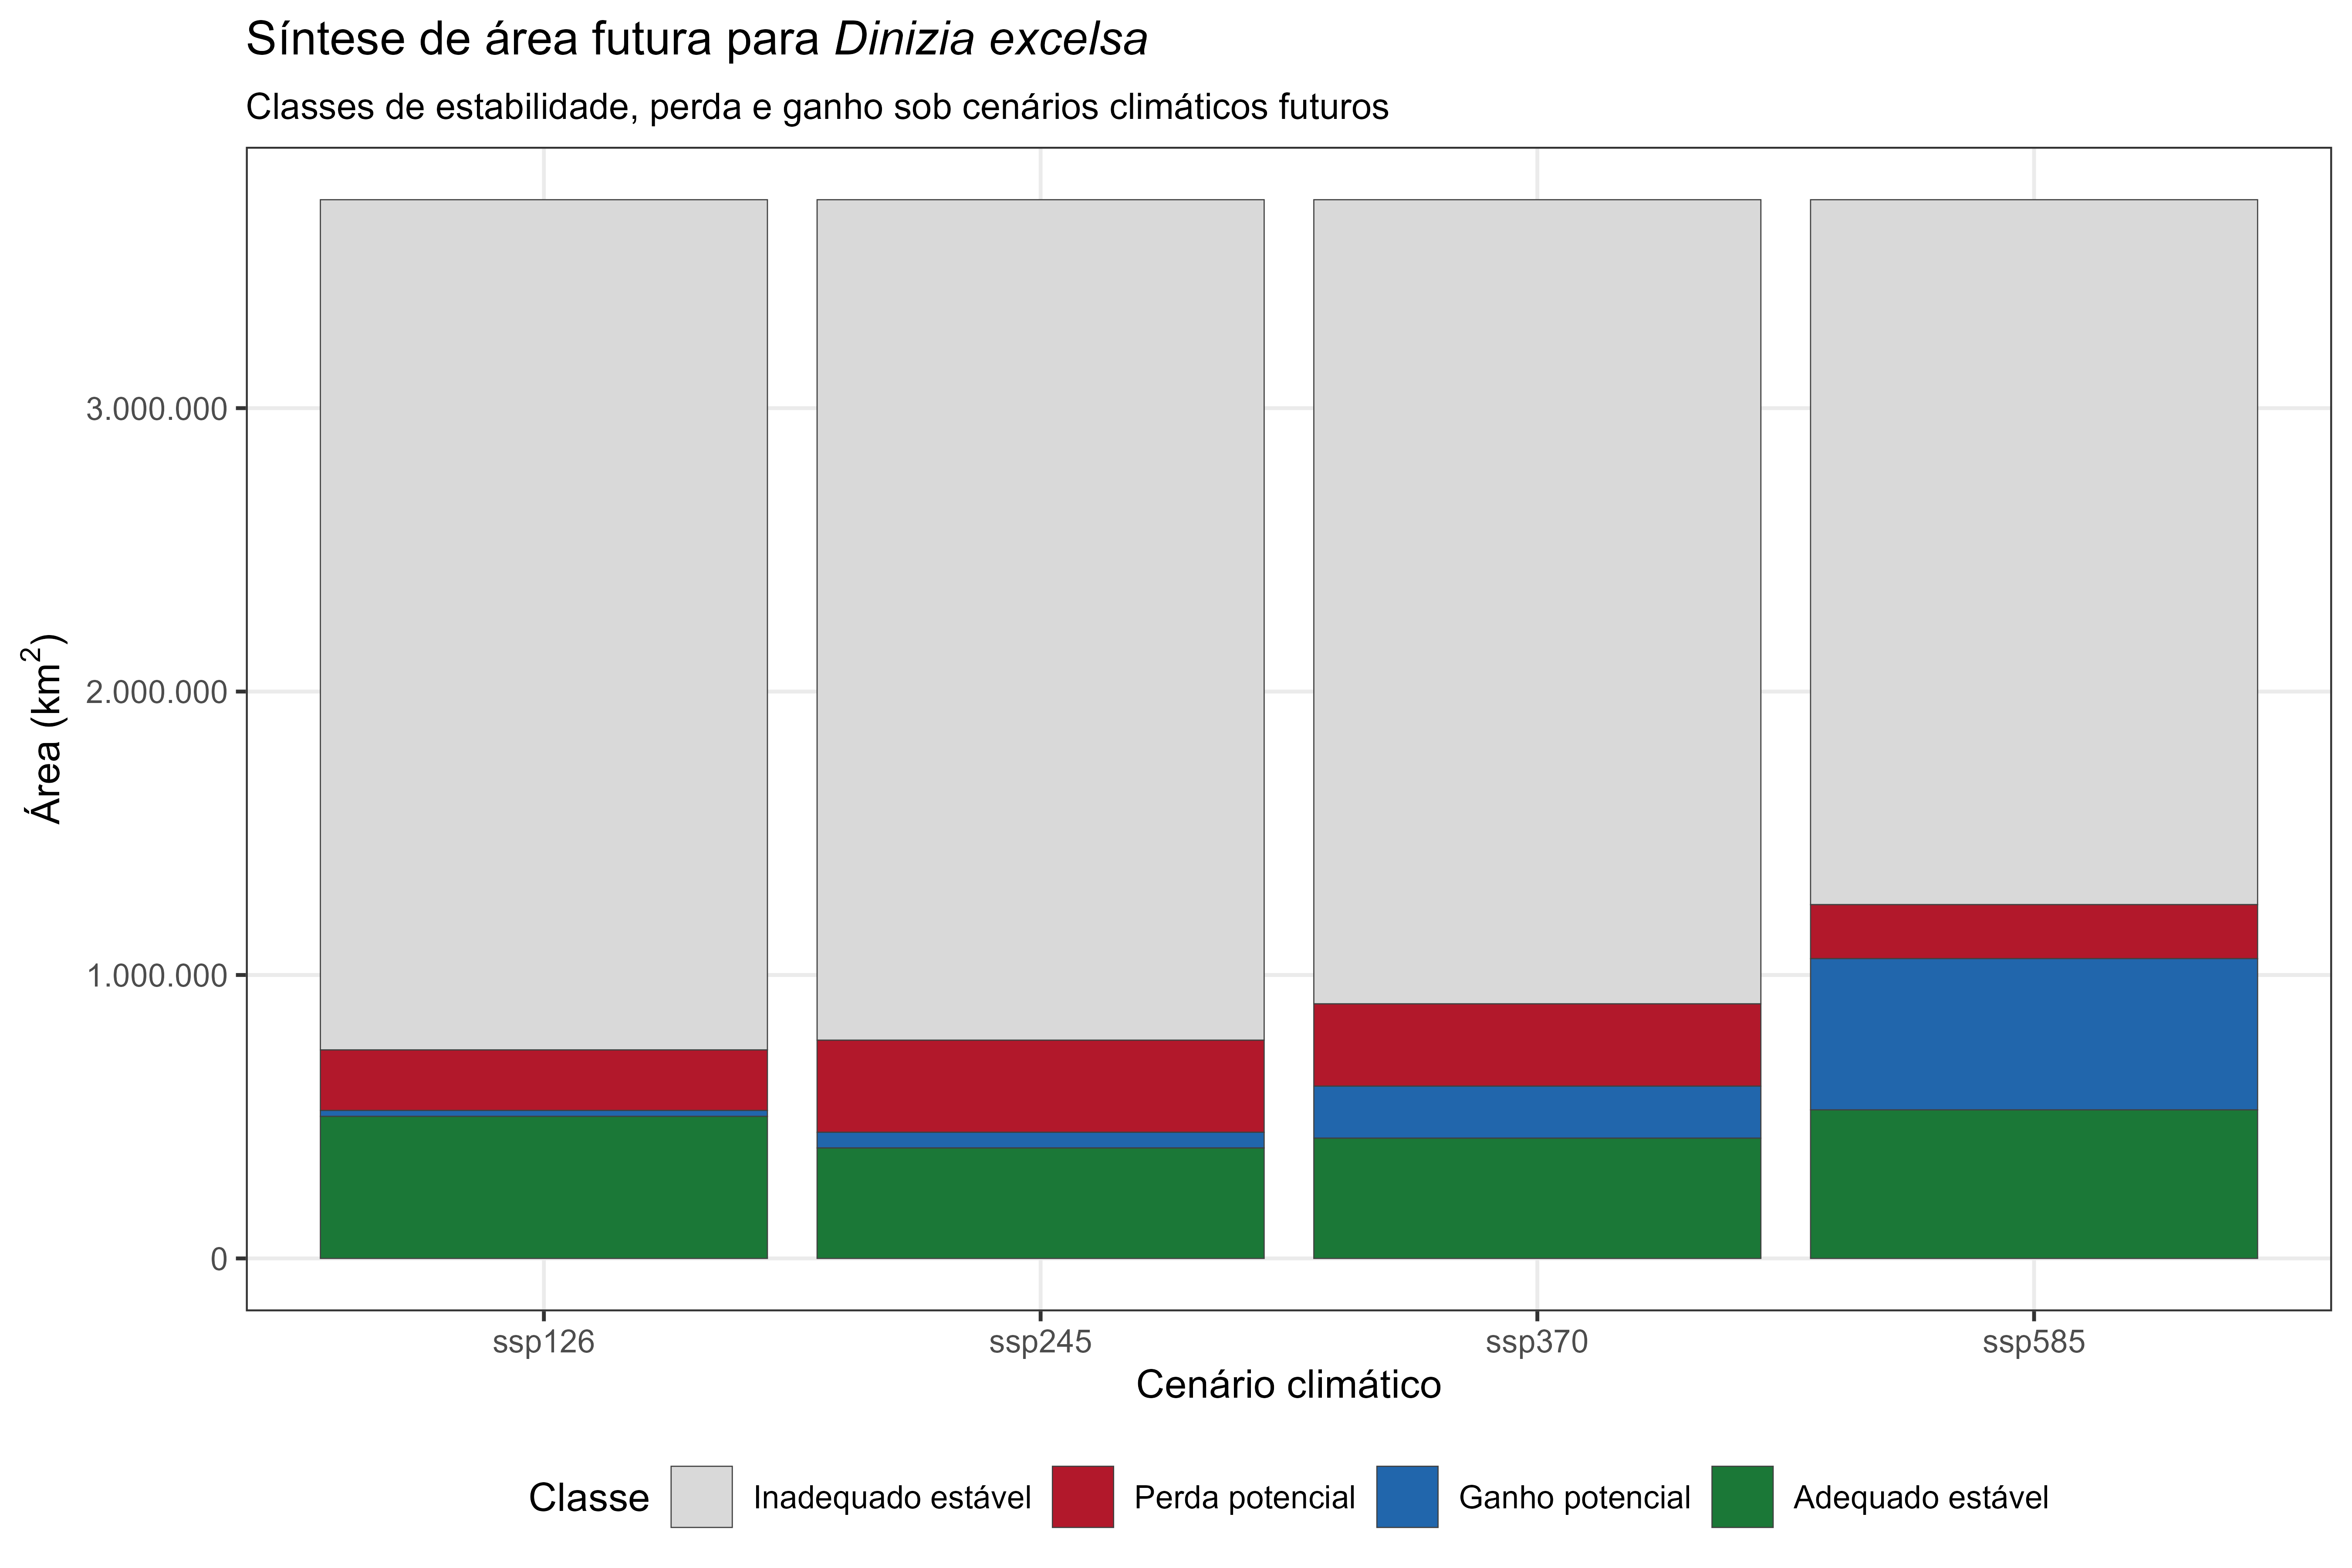
\includegraphics[width=0.88\textwidth]{figuras/unidade13/unidade13_sintese_area_adequada.png}
\caption{Estimated baseline and future suitable area for \textit{Dinizia excelsa} under alternative SSPs.}
\label{fig:unidade13_sintese_area}
\end{figure}

Area summaries should retain the full hierarchy of uncertainty wherever the data permit: algorithm, GCM, SSP, time horizon, replicate or fold, and threshold. Reporting only an ensemble mean can conceal disagreement that is directly relevant to conservation decisions.

\section{Complete pipeline}

\rscriptfile{scripts/unidade13/08_pipeline_projecoes_futuras.R}

\section{Chapter synthesis}

Future climate projections provide conditional evidence about possible changes in environmental suitability under alternative climate trajectories. For \textit{Dinizia excelsa}, they support questions about climatic persistence, potential contraction or expansion, environmental stability, and exposure to warming. They do not, by themselves, predict future occupancy or population viability.

\begin{conceito}[title={\faBook\quad Key message}]
Future SDM outputs are scenarios of environmental suitability, not deterministic forecasts of occurrence. Defensible inference depends on baseline data quality, predictor comparability, explicit scenario design, transferability diagnostics, and propagation of uncertainty across algorithms and climate models.
\end{conceito}

\section{Review exercises}

\begin{enumerate}
\item Distinguish baseline climate data from future climate projections in an SDM workflow.
\item What information is encoded in an SSP-based scenario label such as SSP2--4.5?
\item Why must future predictors match the variables used for model calibration in definition and units, not merely in name?
\item How should positive and negative values of \(\Delta S\) be interpreted?
\item What does climatic stability mean in a comparison of thresholded maps?
\item Why should potential gains not be interpreted as certain future colonization?
\item How can an uncertainty hierarchy improve the conservation use of future projections?
\end{enumerate}

\chapter[Transferability and extrapolation]{Spatial and Temporal Transferability, Extrapolation, MESS, and MOP}

\begin{objetivos}
By the end of this chapter, readers should be able to explain the challenges of spatial and temporal transfer in SDM; distinguish environmental interpolation from extrapolation; calculate and interpret MESS and MOP diagnostics; identify future environments outside the calibration domain; evaluate extrapolation risk in projections for \textit{Dinizia excelsa}; and interpret transferred predictions in conjunction with environmental novelty.
\end{objetivos}

\section{Introduction}

Species distribution models are often calibrated under contemporary conditions and transferred to another region or period, including future climates, paleoclimates, or distinct geographic domains. Transfer is among the most valuable applications of SDM and among the most vulnerable to failure \parencite{peterson2011,araujo2012,yates2018transferability,zurell2020benchmarking}.

Environmental interpolation occurs when projection conditions are represented adequately within the calibration domain. Extrapolation occurs when one or more predictor values, or their multivariate combinations, lie outside that experience. In extrapolative environments, an algorithm may still return a numerical prediction, but its ecological support is weak and its behavior may be governed by model form, clamping rules, or terminal responses rather than empirical information.

\begin{conceito}[title={\faBook\quad Interpolation versus extrapolation}]
Interpolation applies a model within an environmental domain represented during calibration. Extrapolation applies it to values or multivariate combinations not represented by the calibration data. Geographic distance alone does not define either condition: a distant region may be environmentally analogous, whereas a nearby period may contain novel environments.
\end{conceito}

\section{Spatial and temporal transfer}

Spatial transfer applies a model calibrated in one region to another region. Temporal transfer applies a model calibrated in one period to past or future conditions. Reliability depends not only on environmental similarity, but also on the stability of the occurrence--environment relationship and on differences in sampling, accessibility, biotic interactions, land use, and evolutionary or demographic processes.

\begin{atencao}[title={\faExclamationTriangle\quad Transferred projections require novelty diagnostics}]
Future or paleoclimatic suitability maps should not be interpreted in isolation. They must be paired with environmental-similarity diagnostics and with an explicit account of algorithmic extrapolation settings, including clamping where applicable.
\end{atencao}

\section{MESS: Multivariate Environmental Similarity Surface}

MESS compares each projection cell with the distribution of predictor values in a chosen reference sample from the calibration environment. Negative values identify at least one predictor outside its reference range; nonnegative values indicate that each individual predictor lies within its observed range. This does not guarantee that the multivariate combination is well represented. Results also depend on how the calibration reference is sampled, scaled, and masked.

\rscriptfile{scripts/unidade14/01_estrutura_pastas.R}

\rscriptfile{scripts/unidade14/02_calcular_mess_futuro.R}

\begin{figure}[H]
\centering
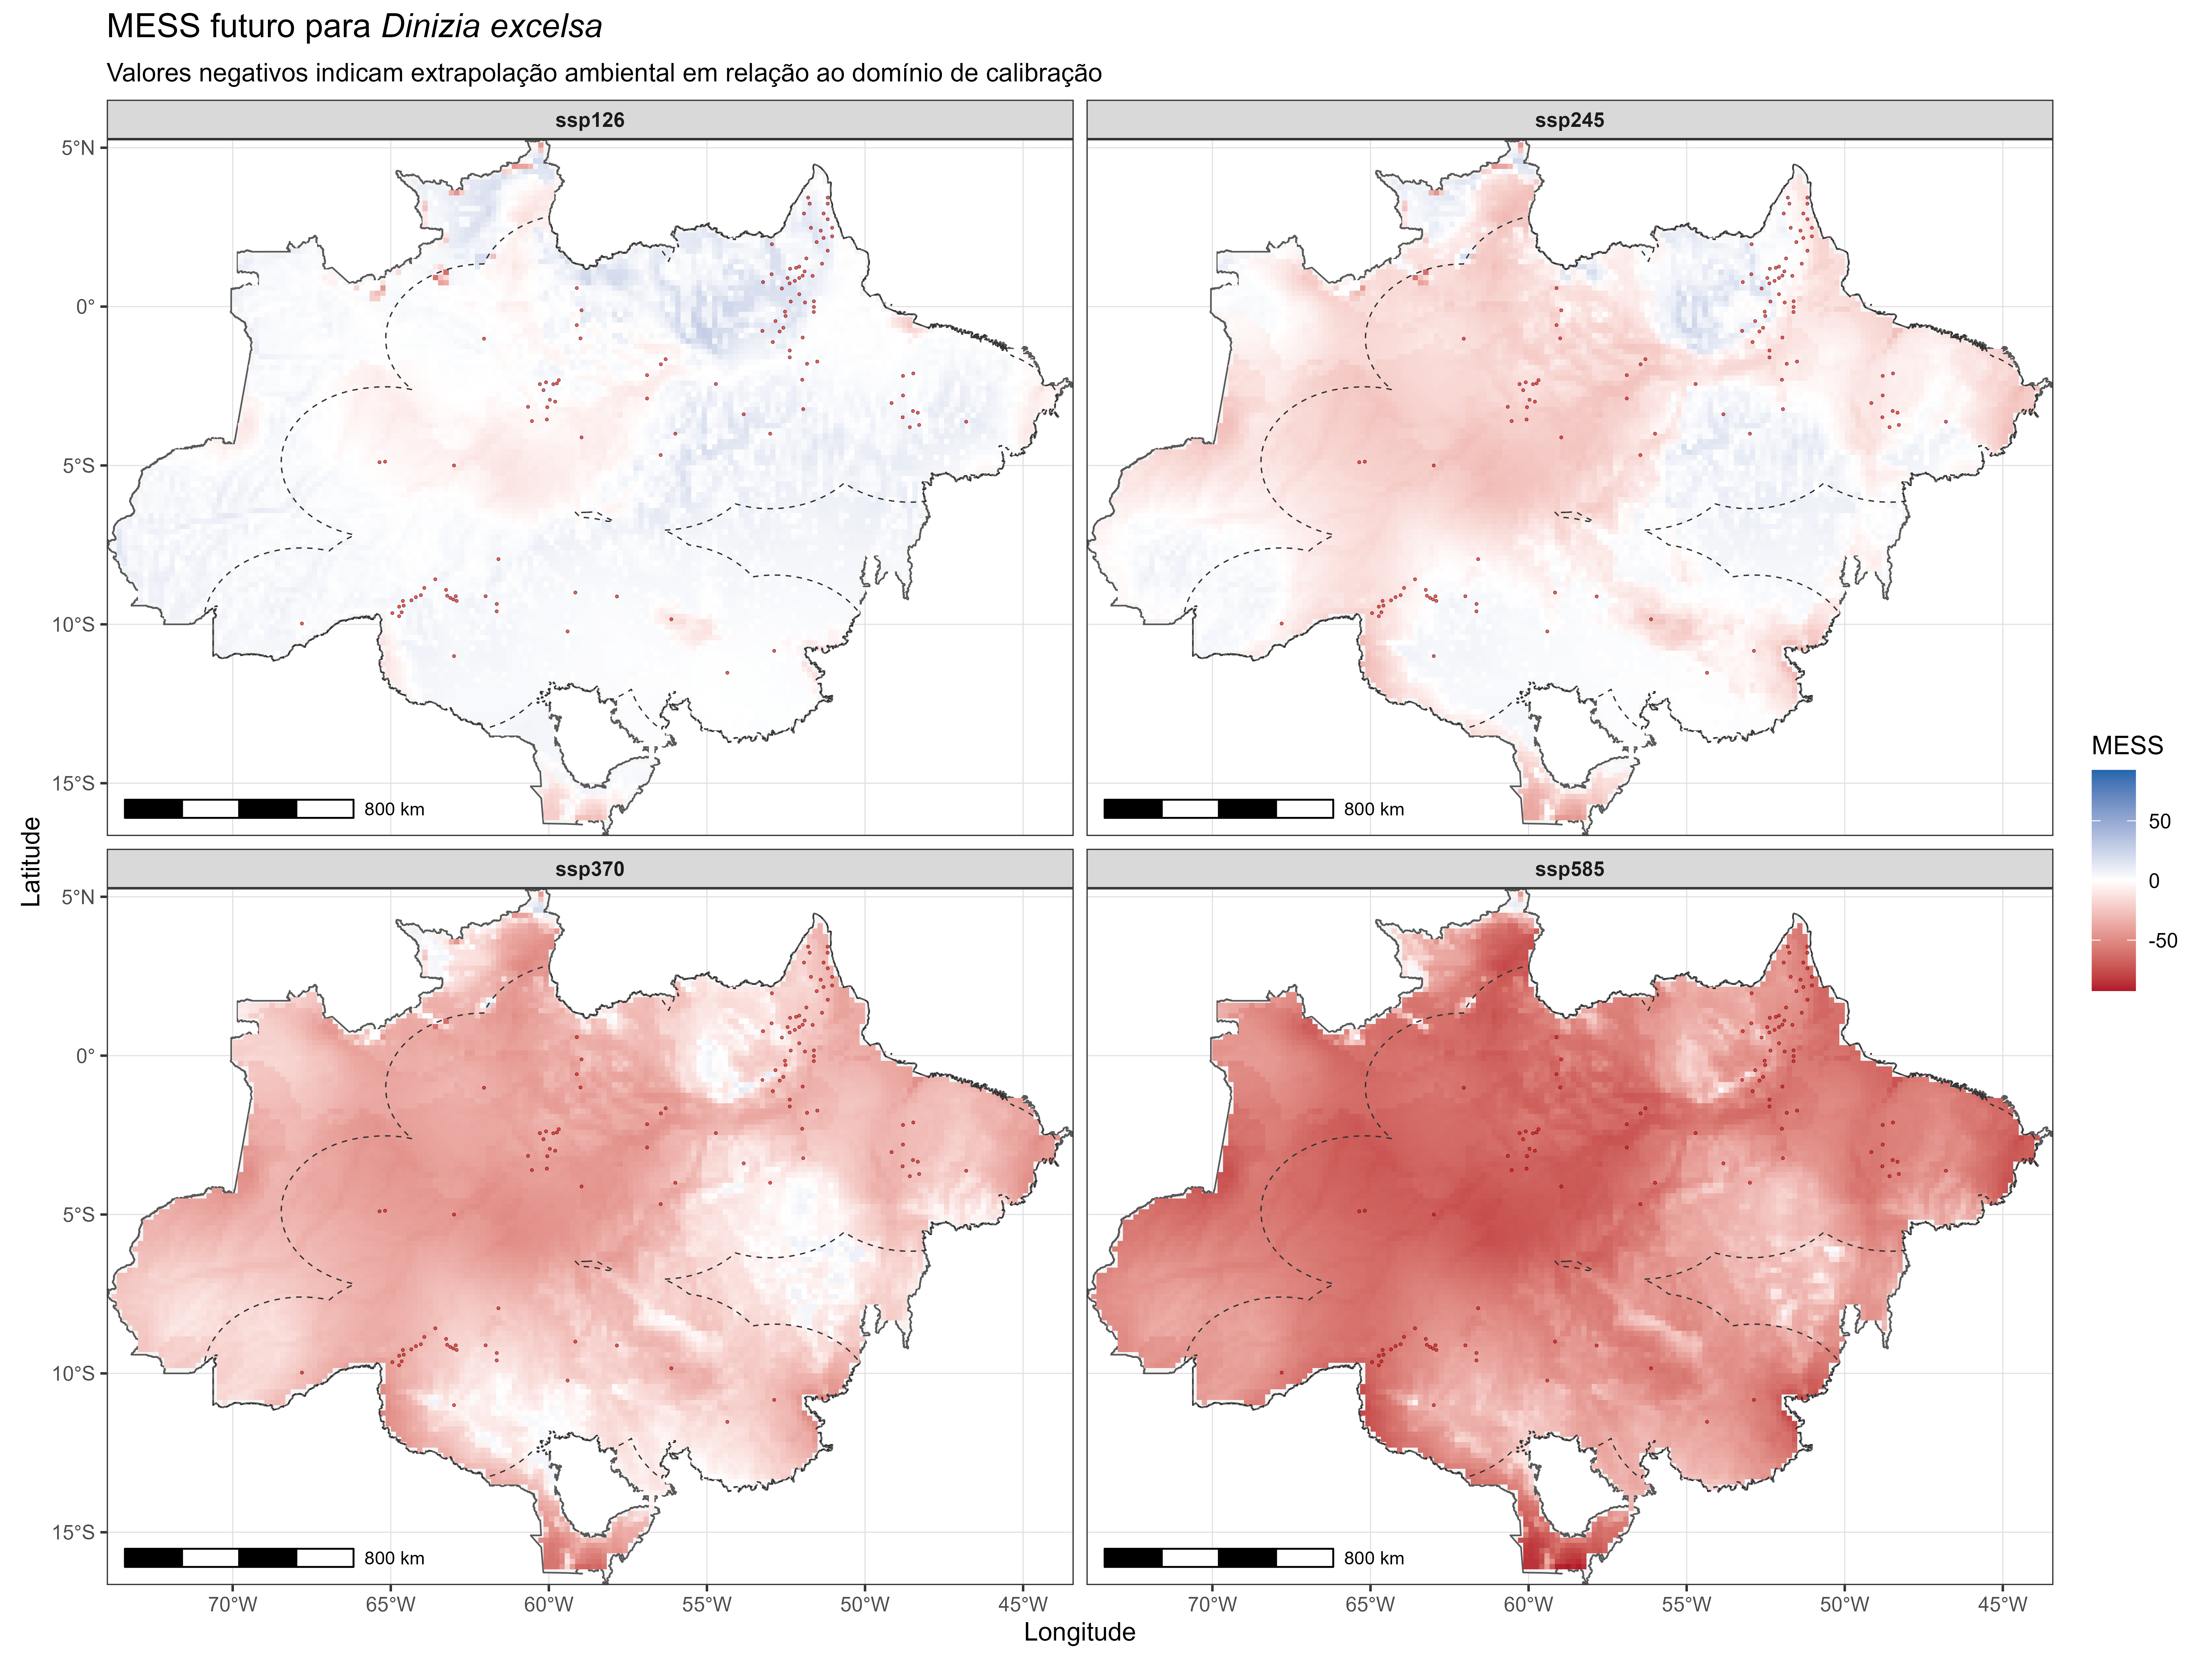
\includegraphics[width=0.96\textwidth]{figuras/unidade14/unidade14_mess_cenarios.png}
\caption{MESS diagnostics for future projections of \textit{Dinizia excelsa}. Negative values identify univariate extrapolation relative to the calibration domain.}
\label{fig:unidade14_mess}
\end{figure}

\section{The most dissimilar variable in MESS}

In addition to the similarity score, MESS can identify the variable contributing the greatest dissimilarity in each cell. This diagnostic helps determine whether future novelty is driven primarily by temperature, precipitation, seasonality, or another predictor. It should not be interpreted as a causal limiting factor for the species; it identifies a statistical boundary of the calibration domain.

\rscriptfile{scripts/unidade14/03_variavel_limitante_mess.R}

\begin{figure}[H]
\centering
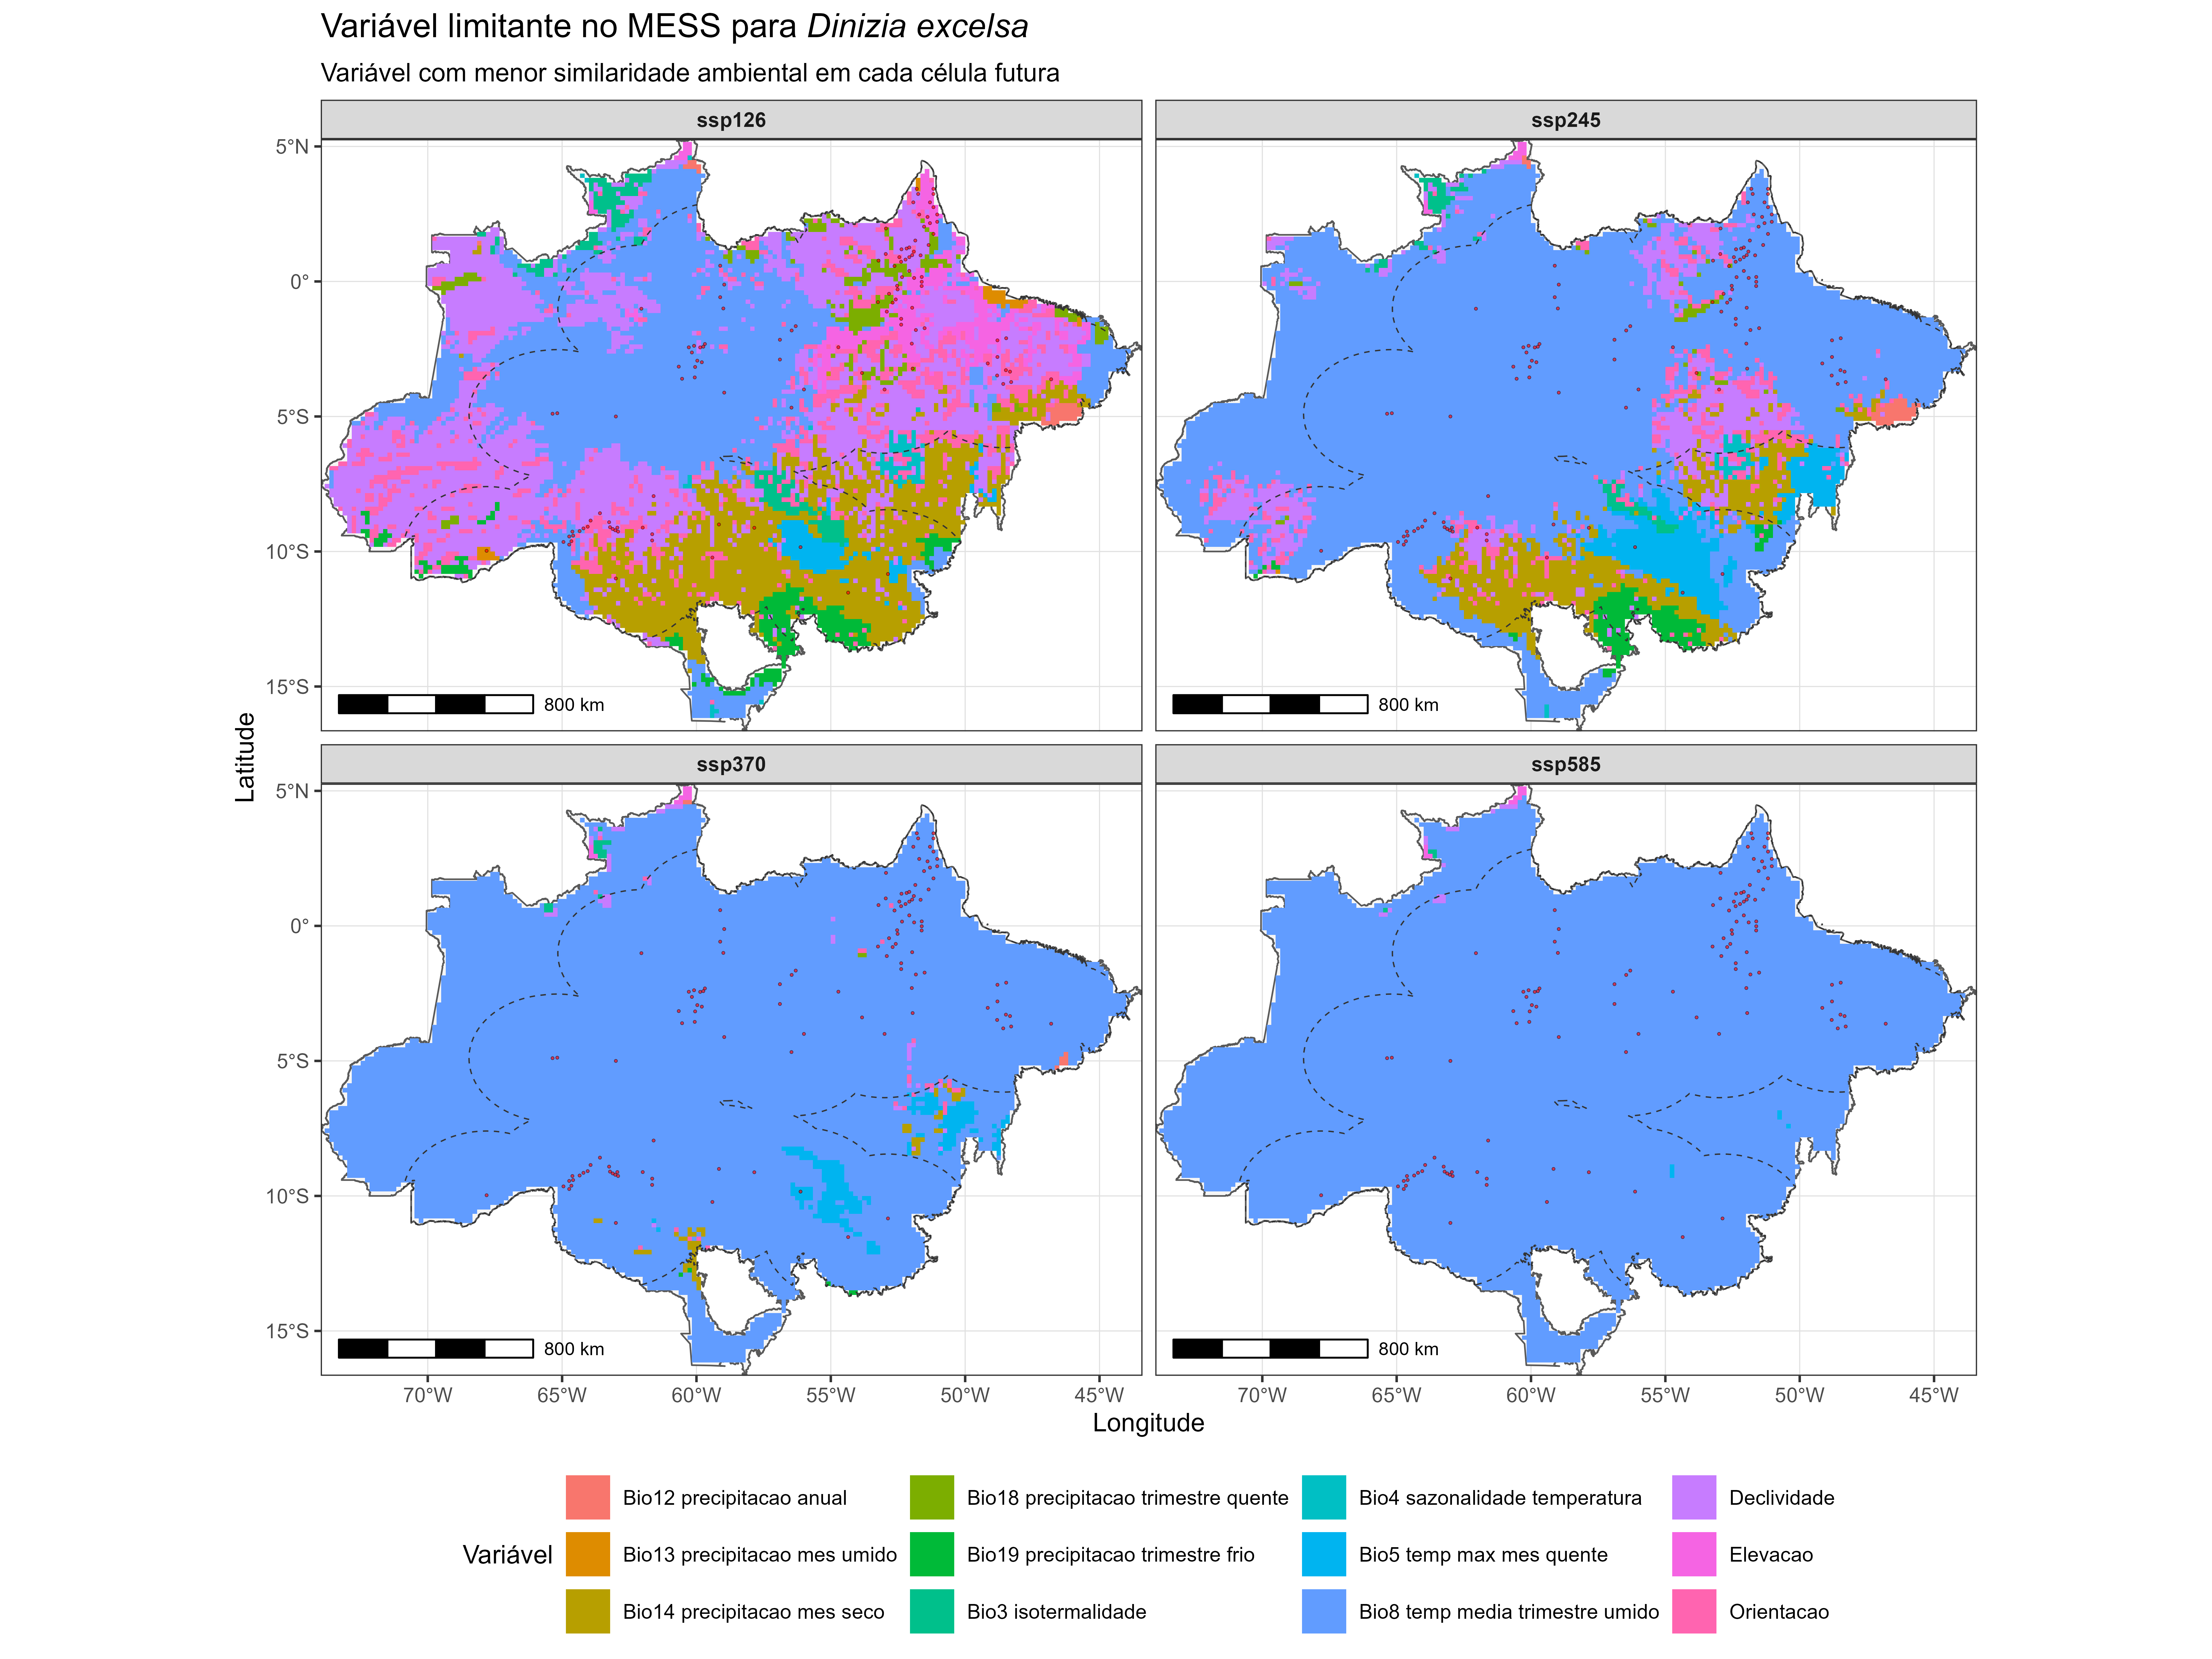
\includegraphics[width=0.96\textwidth]{figuras/unidade14/unidade14_variavel_limitante_mess.png}
\caption{Predictor contributing the greatest environmental dissimilarity in the future MESS diagnostic.}
\label{fig:unidade14_limitante}
\end{figure}

\section{MOP: Mobility-Oriented Parity}

MOP evaluates multivariate environmental similarity between calibration and projection domains using distances in environmental space. It is designed to identify strict extrapolation and to rank similarity among analogous conditions \parencite{owens2013constraints}. Unlike a range-by-range diagnostic, it can reveal novel combinations even when individual predictor values remain within their marginal calibration ranges. Predictor standardization, correlation, reference sampling, and distance definition influence the resulting surface and must be documented.

\rscriptfile{scripts/unidade14/04_calcular_mop_futuro.R}

\begin{figure}[H]
\centering
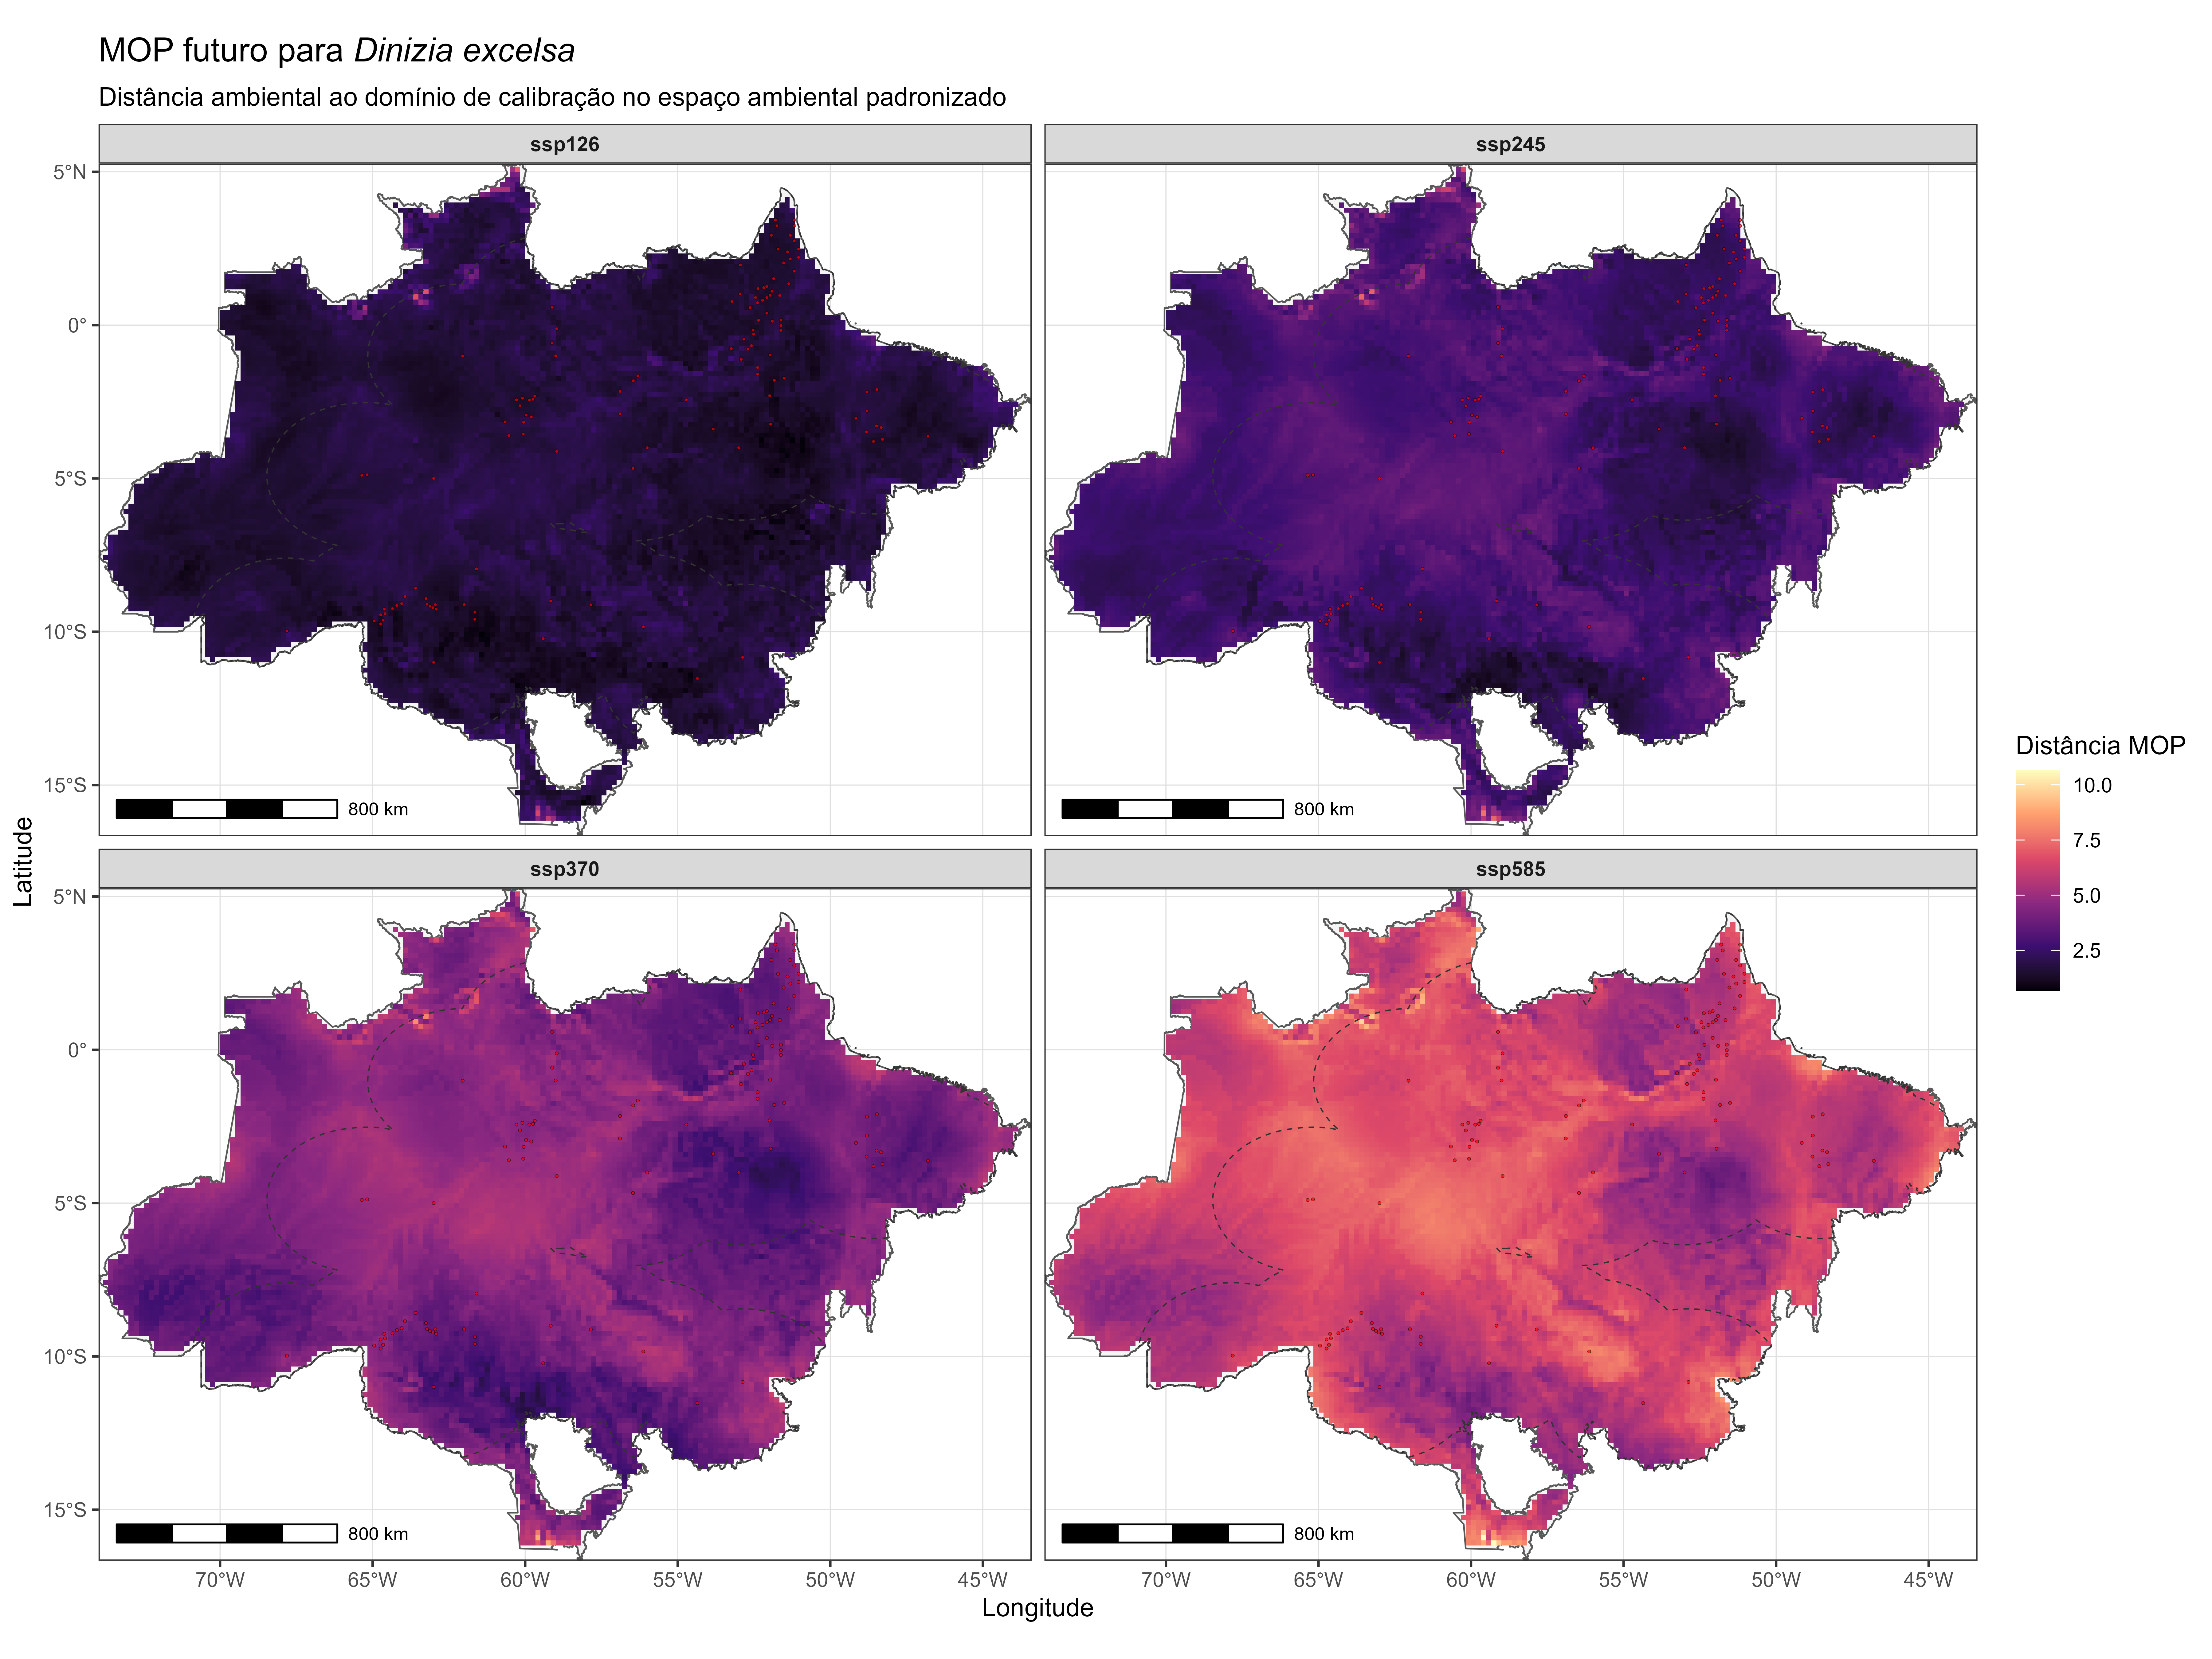
\includegraphics[width=0.96\textwidth]{figuras/unidade14/unidade14_mop_cenarios.png}
\caption{Simplified MOP diagnostics for future scenarios. Under the distance-oriented implementation used here, larger values indicate greater environmental distance from the calibration domain.}
\label{fig:unidade14_mop}
\end{figure}

\begin{atencao}[title={\faExclamationTriangle\quad Verify the direction of the MOP scale}]
MOP software and plotting workflows may express similarity, distance, or rescaled parity in different directions. Always verify the implementation before labeling low or high values as novel; the map legend and methods must state the convention used.
\end{atencao}

\section{Suitability under extrapolation}

Future suitability is now combined with MESS and MOP outputs to locate cells predicted as suitable under novel environmental conditions. Such cells are not necessarily unsuitable, but the evidence supporting their estimates is weaker because the model is being asked to generalize beyond its calibration experience.

\rscriptfile{scripts/unidade14/05_adequabilidade_extrapolacao.R}

\begin{figure}[H]
\centering
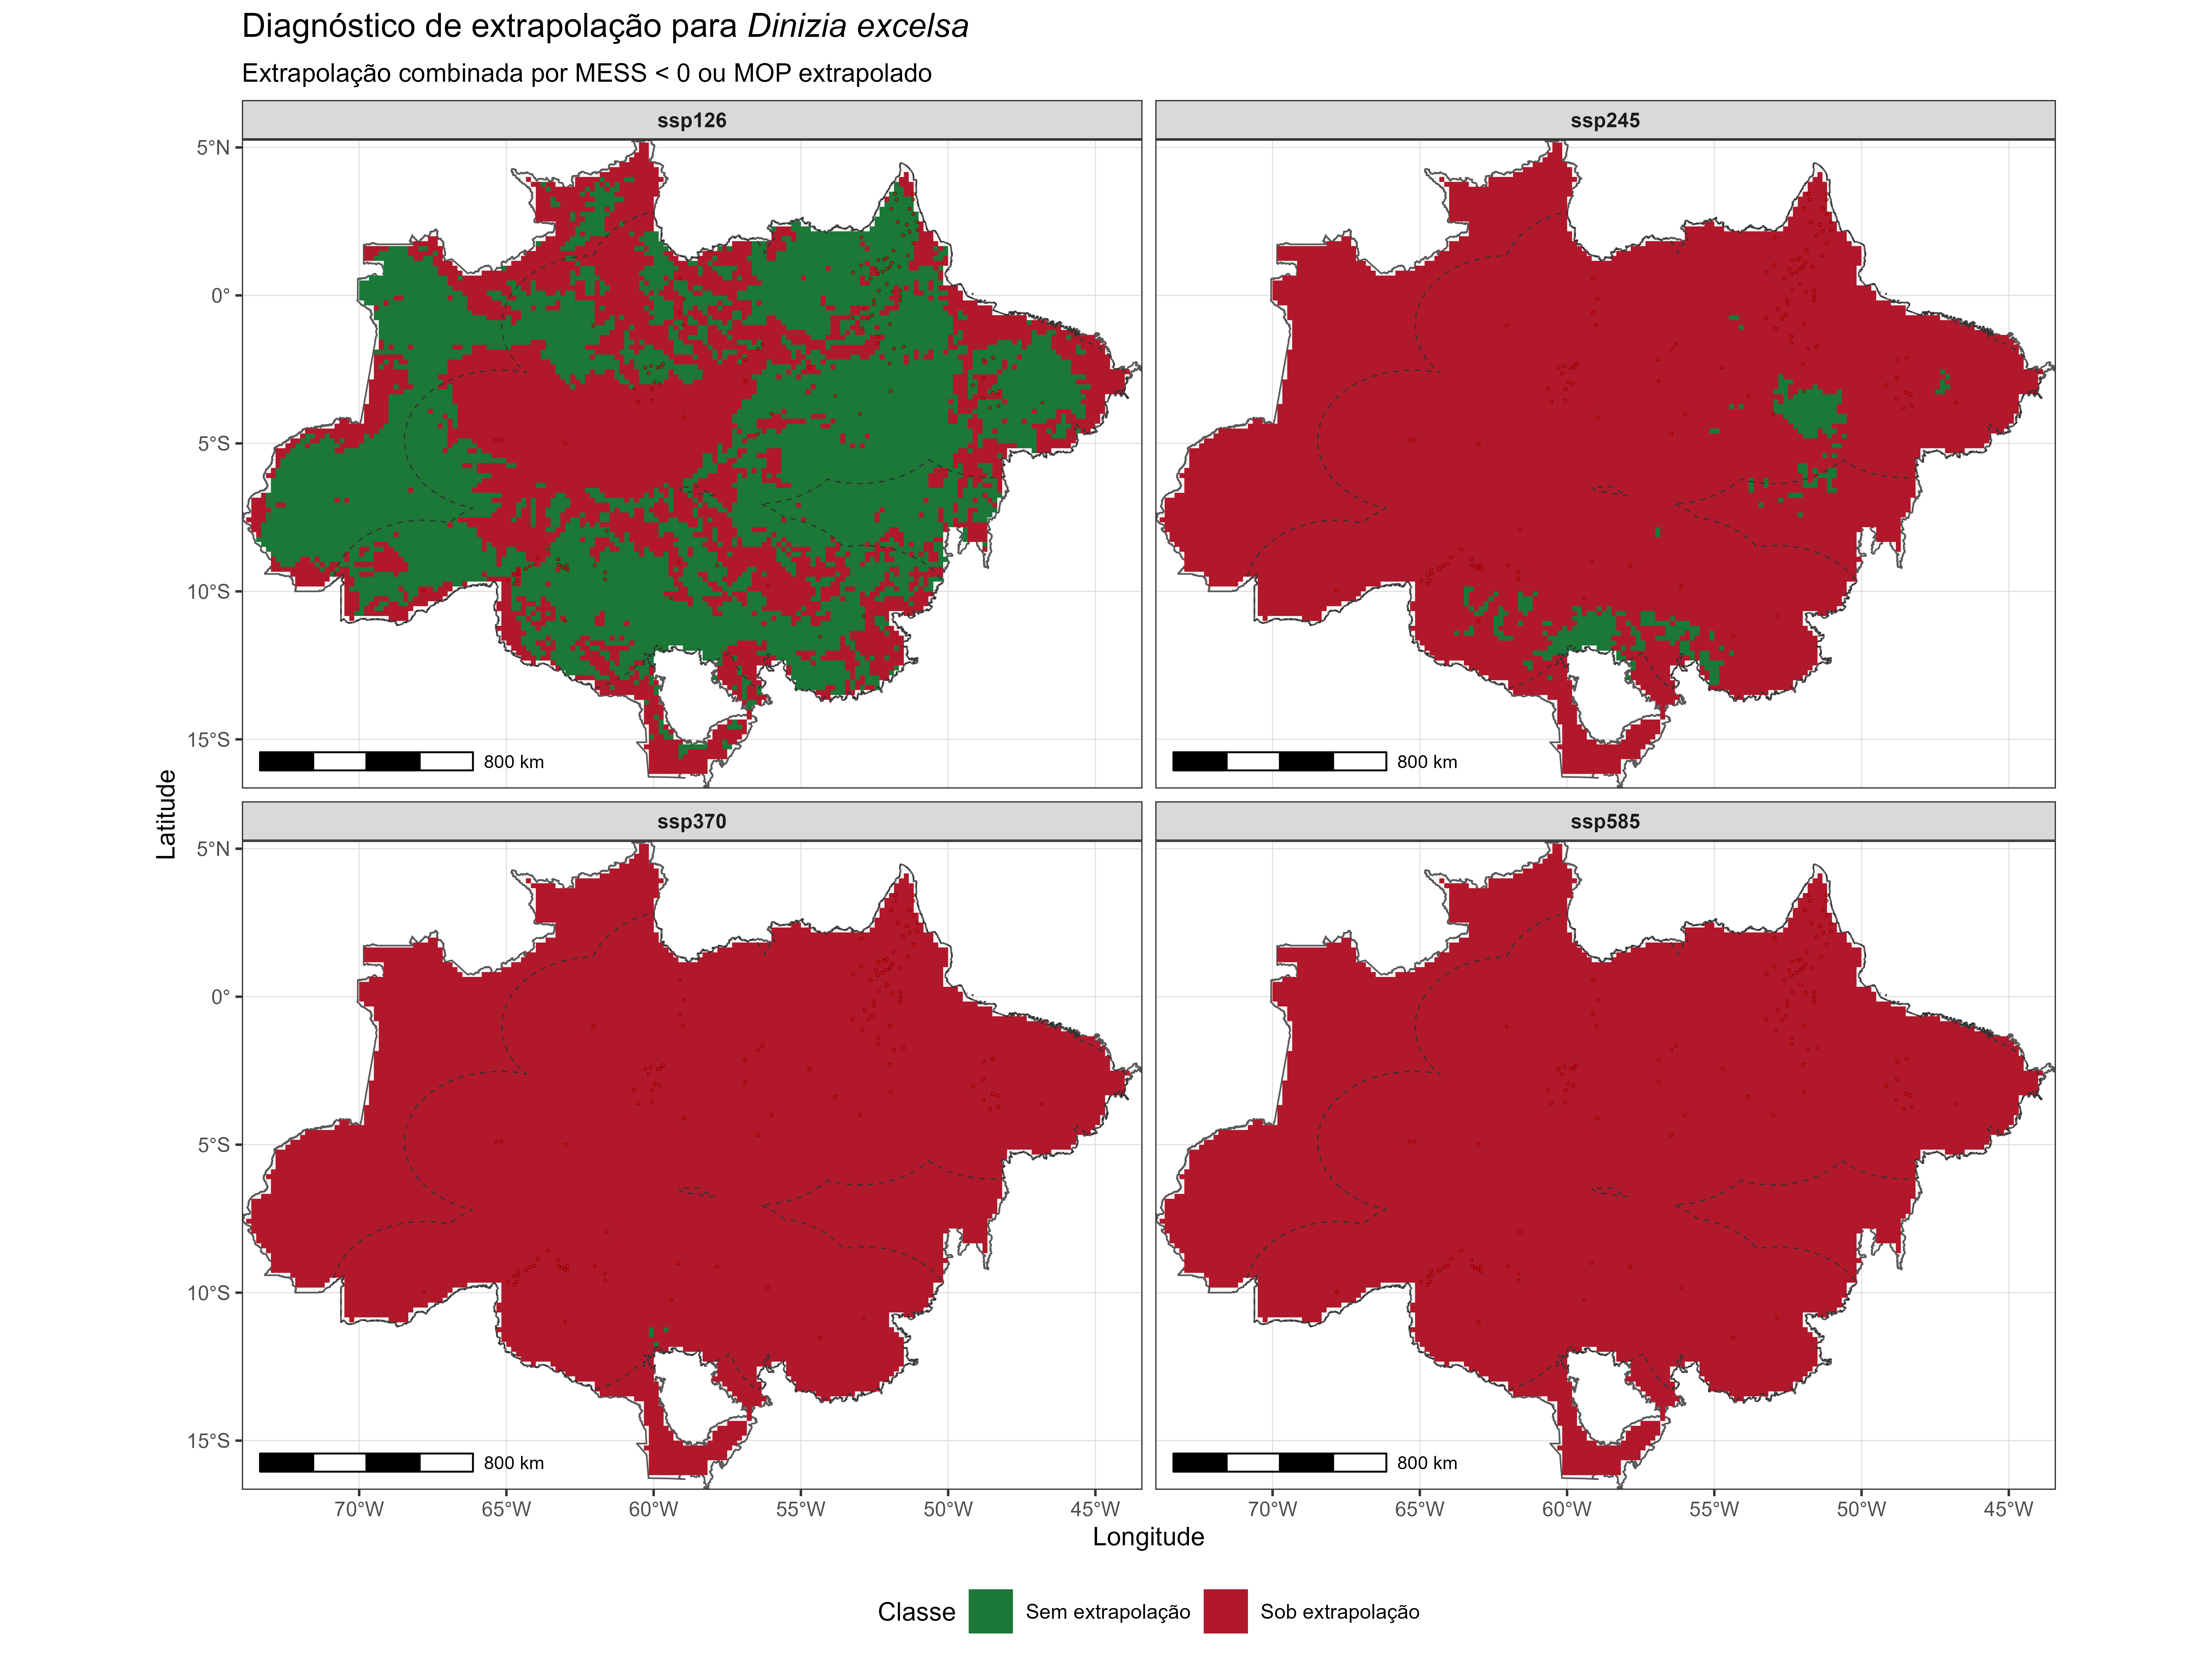
\includegraphics[width=0.96\textwidth]{figuras/unidade14/unidade14_adequabilidade_extrapolacao.png}
\caption{Future suitability combined with diagnostics of environmental extrapolation.}
\label{fig:unidade14_adequabilidade_extrapolacao}
\end{figure}

Novelty masks can be used to flag, summarize, or exclude projections, but these choices answer different questions. Masking prevents unsupported cells from appearing as ordinary predictions; retaining them with prominent uncertainty flags preserves information about where the model is being challenged. The decision should be declared before interpretation and applied consistently.

\section{Synthesis of extrapolation risk}

\rscriptfile{scripts/unidade14/06_sintese_extrapolacao.R}

\begin{figure}[H]
\centering
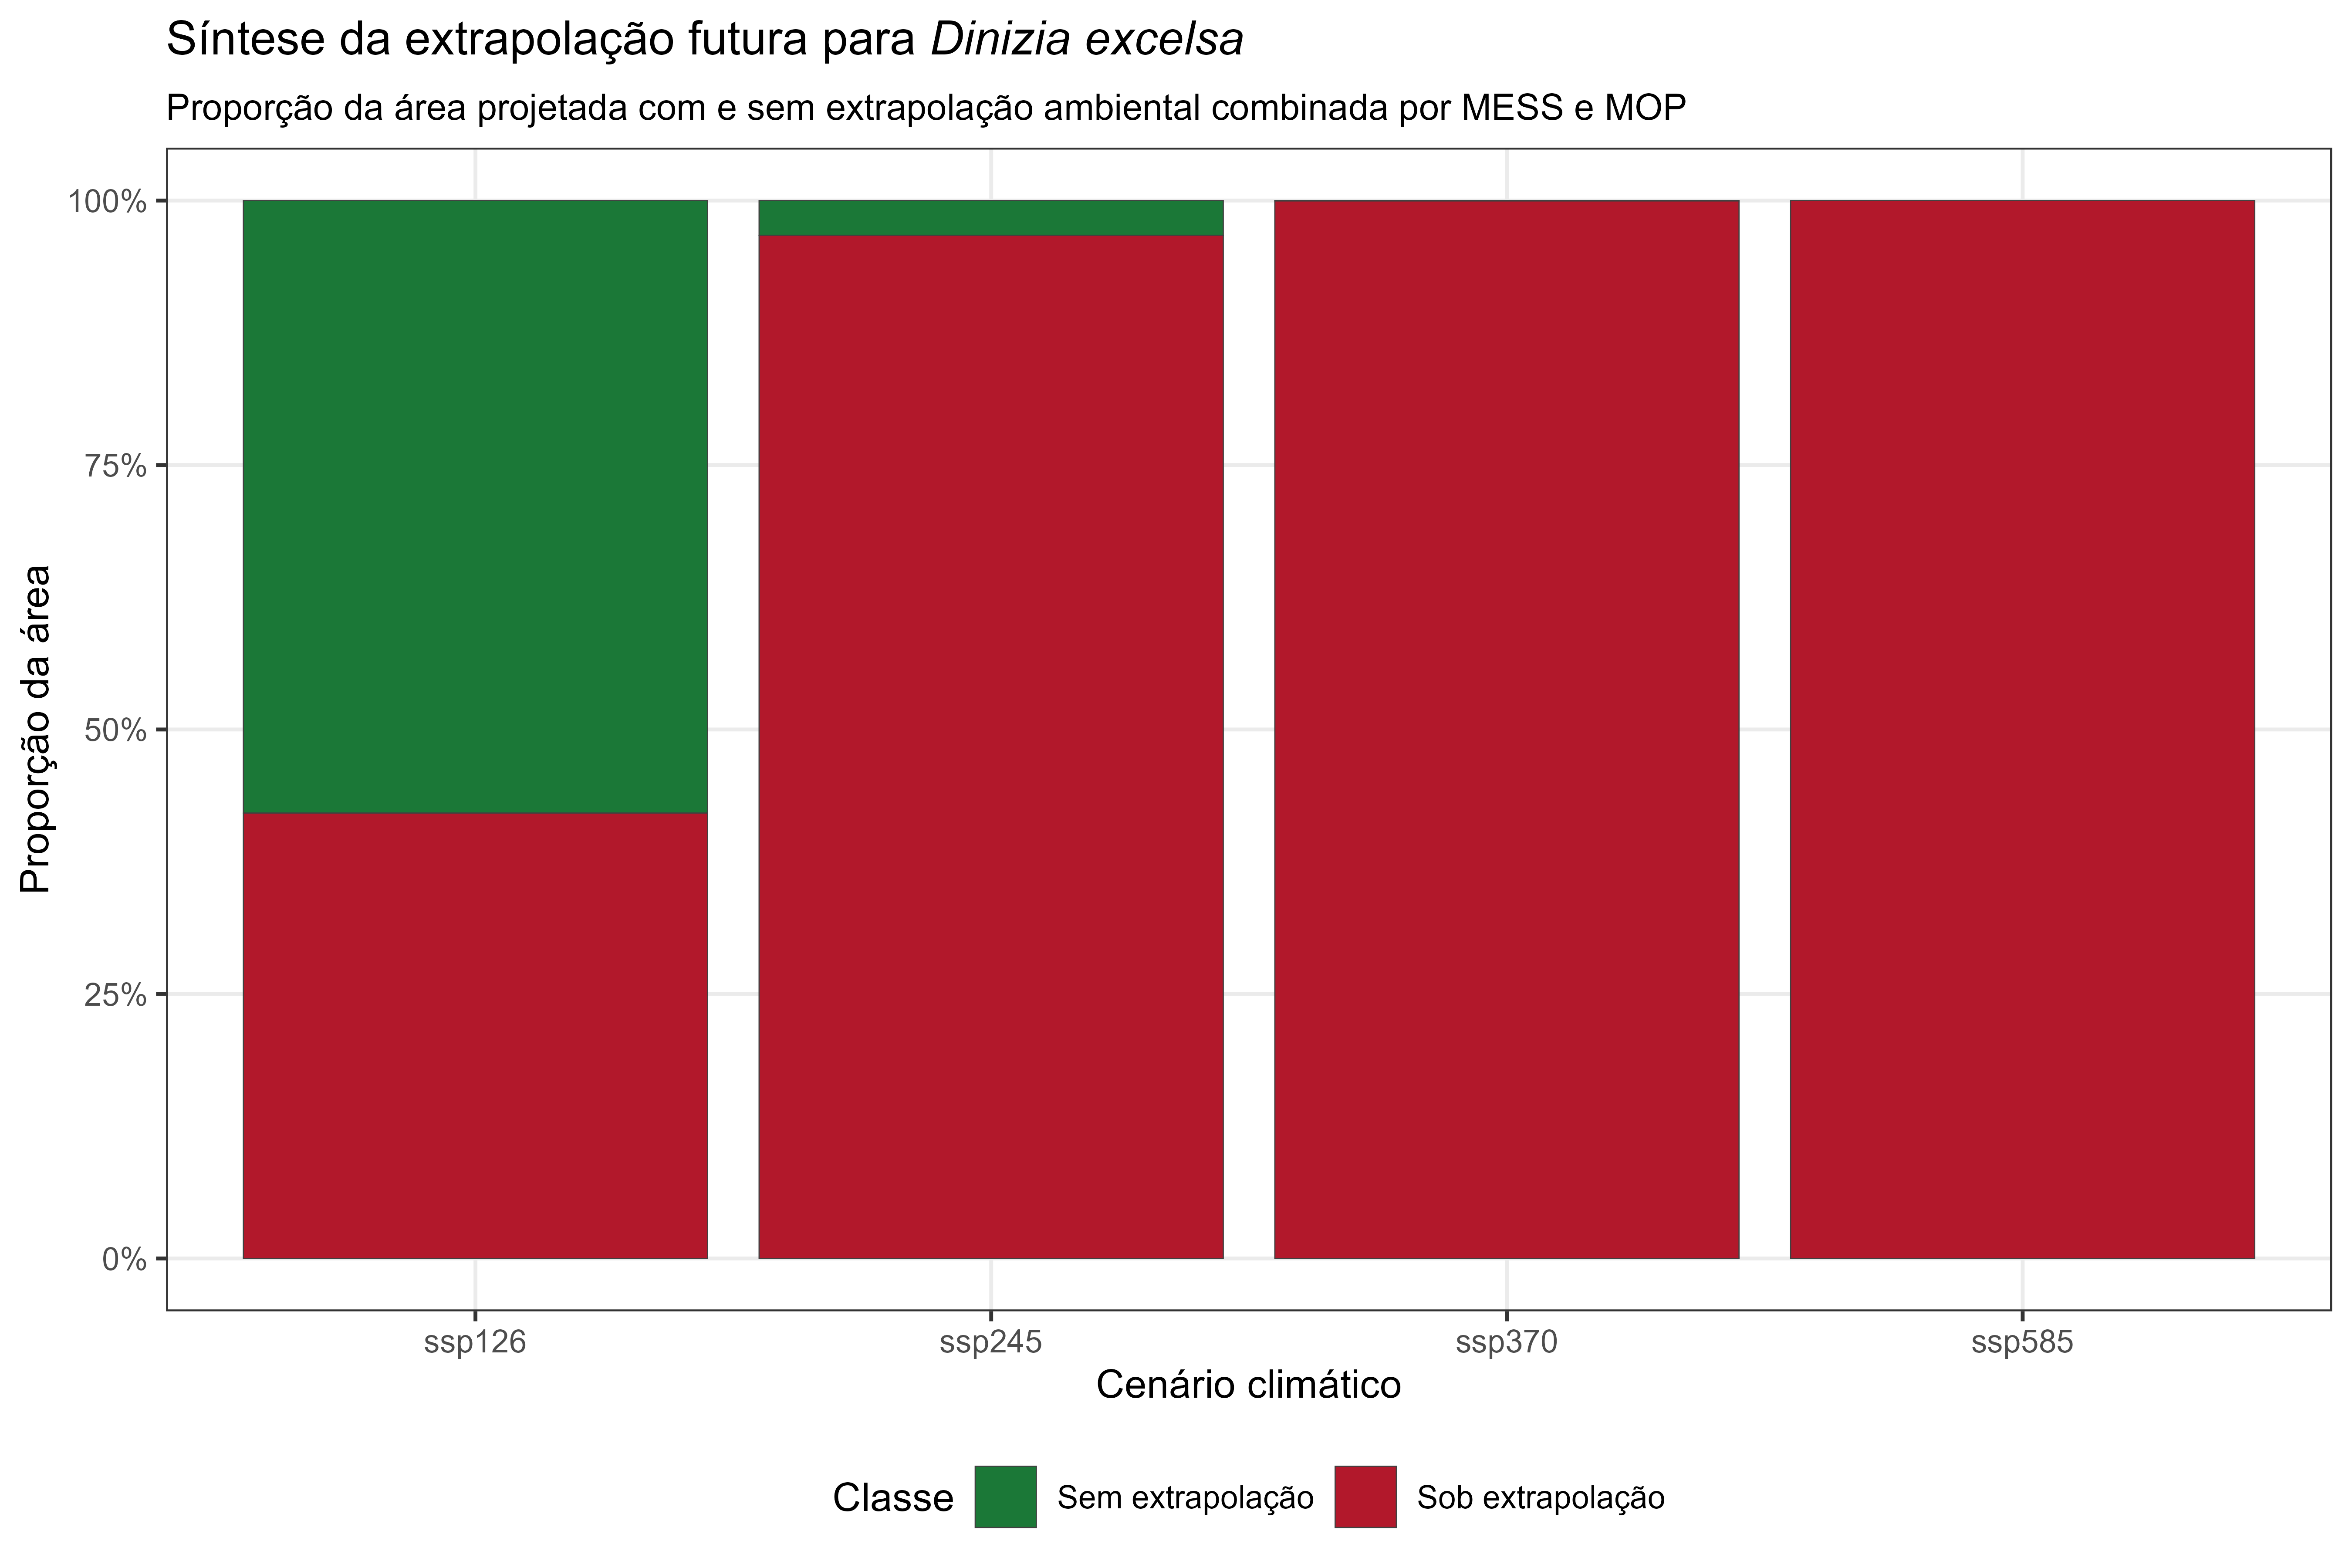
\includegraphics[width=0.88\textwidth]{figuras/unidade14/unidade14_sintese_extrapolacao.png}
\caption{Proportion of the future projection area classified as environmentally extrapolative under each SSP.}
\label{fig:unidade14_sintese}
\end{figure}

The proportion of novel area should be reported relative to an explicit denominator, such as the complete projection extent, the accessible area, or cells classified as suitable. These denominators represent different ecological questions and should not be conflated.

\section{Complete pipeline}

\rscriptfile{scripts/unidade14/07_pipeline_transferencia_extrapolacao.R}

\section{Chapter synthesis}

Spatial and temporal transfer is essential to climate-change and historical SDM applications, but it requires rigorous novelty diagnostics. For \textit{Dinizia excelsa}, MESS and MOP identify environments in which future estimates deserve greater caution. Neither diagnostic measures predictive error directly; instead, they identify departures from the conditions that supported calibration.

\begin{conceito}[title={\faBook\quad Key message}]
Transferred projections are most defensible when environmental novelty is quantified and displayed. High predicted suitability under strong extrapolation is an uncertain hypothesis, not robust evidence of future persistence.
\end{conceito}

\section{Review exercises}

\begin{enumerate}
\item Distinguish environmental interpolation from extrapolation.
\item What does a negative MESS value indicate, and what does a nonnegative value fail to guarantee?
\item How do MESS and MOP differ conceptually?
\item Why can an algorithm predict high suitability in a strongly extrapolative environment?
\item What information should accompany a novelty mask in a published map?
\item Why is temporal transfer particularly sensitive to assumptions about ecological stationarity?
\item How would you combine suitability, MESS, MOP, and dispersal constraints when prioritizing conservation areas?
\end{enumerate}


\chapter[Paleoclimate and historical climatic niches]{Paleoclimate, Historical Climatic Niches, and Distributional Reconstruction}

\begin{objetivos}
By the end of this chapter, readers should be able to explain how paleoclimatic data are used in SDM; recognize the mid-Holocene, Last Glacial Maximum, and Last Interglacial; harmonize paleoclimatic predictors with baseline model inputs; project models for \textit{Dinizia excelsa} to past climates; evaluate historical climatic stability; identify candidate areas of long-term suitability; and interpret paleoclimate projections as biogeographic hypotheses rather than direct evidence of past occurrence.
\end{objetivos}

\section{Introduction}

The contemporary distribution of an Amazonian tree species reflects both present-day ecological processes and a deeper climatic history. Past changes in temperature, precipitation, seasonality, forest connectivity, and environmental stability may have influenced population persistence, expansion, contraction, and spatial genetic structure.

In SDM, models calibrated with contemporary data can be transferred to reconstructed climates such as the mid-Holocene, Last Glacial Maximum, and Last Interglacial. These projections support hypotheses about climatic stability, potential refugia, historical connectivity, and niche conservatism. Their interpretation requires the same transferability safeguards used for future projections, together with recognition that uncertainties increase backward through climate reconstruction, model choice, and ecological assumptions.

\begin{conceito}[title={\faBook\quad Historical climatic niche}]
A historical climatic-niche projection represents past environmental conditions that a contemporary fitted model classifies as compatible with the species' estimated climatic association. It does not reconstruct the complete historical niche, demonstrate occupancy, or establish population continuity.
\end{conceito}

\section{A climatic timeline from the past to possible futures}

Paleoclimate modeling reconstructs potential distributions under past environmental conditions, whereas future projections explore responses under alternative climate trajectories. Together, these approaches connect historical biogeography, climatic stability, candidate refugia, and future vulnerability.

Here, the modeled climatic association of \textit{Dinizia excelsa} is interpreted along a timeline comprising widely used paleoclimatic periods, baseline conditions, and future GCM scenarios. The comparison asks whether currently suitable areas may also have been suitable in the past and whether they remain suitable under specified future conditions.

\begin{center}
\fbox{
\begin{minipage}{0.90\textwidth}
\centering
\textbf{Climatic timeline used to interpret model projections}

\vspace{0.4cm}

\small
\setlength{\tabcolsep}{4pt}
\begin{tabular}{p{0.12\textwidth}p{0.25\textwidth}p{0.45\textwidth}}
\toprule
\textbf{Time} & \textbf{Period/scenario} & \textbf{Ecological interpretation} \\
\midrule
about 130 ka & Last Interglacial (LIG) & A warm interval before the last glacial cycle, useful for exploring model responses under a climate distinct from the present. \\
about 21 ka & Last Glacial Maximum (LGM) & The coldest phase of the last glacial cycle, associated with major changes in tropical climates and vegetation. \\
about 6 ka & Mid-Holocene & A postglacial interval used to examine relatively recent climatic reorganization and stability. \\
baseline & Contemporary reference & The climatic reference period associated with model calibration or baseline interpretation. \\
2050 & SSP1--2.6 and SSP5--8.5 & Mid-century projections under contrasting forcing pathways. \\
2070 & SSP1--2.6 and SSP5--8.5 & Later-century projections under contrasting forcing pathways. \\
\bottomrule
\end{tabular}
\end{minipage}
}
\end{center}

This timeline is a conceptual framework for comparing stability, loss, gain, and displacement of climatically suitable areas across time slices. Persistent modeled suitability can identify candidates for climatic stability, but a biogeographic refugium requires corroboration from independent evidence such as fossils, phylogeography, population genetics, paleoecology, or historical demography. Areas suitable only in one period should be interpreted especially cautiously when environmental novelty is high.

\begin{conceito}[title={\faBook\quad Temporal SDM}]
Integrating paleoclimate, baseline climate, and future scenarios turns SDM into a comparative temporal framework. The question expands from where a species may find suitable conditions today to how modeled suitability, exposure, and potential persistence vary across time.
\end{conceito}

\section{Relevant paleoclimatic periods}

This chapter considers three principal time slices:

\begin{itemize}
\item the mid-Holocene, approximately 6 thousand years before present;
\item the Last Glacial Maximum, approximately 21 thousand years before present;
\item the Last Interglacial, commonly represented by a time slice around 120--130 thousand years before present, depending on the climate product.
\end{itemize}

These periods represent distinct states of the Earth system and allow us to ask whether areas currently suitable for \textit{Dinizia excelsa} were also classified as climatically suitable under reconstructed past conditions. Exact ages and temporal averaging must follow the metadata of the selected paleoclimate dataset.

\begin{atencao}[title={\faExclamationTriangle\quad Paleoclimate projections are hypotheses}]
Paleoclimate SDMs do not demonstrate that a species occurred in a projected cell. They identify locations that may have been climatically suitable under assumptions of model transferability, partial niche conservatism, adequate paleoclimate reconstruction, and absence of unmodeled dispersal or biotic constraints.
\end{atencao}

\section{Preparing paleoclimatic layers}

Paleoclimatic layers must be harmonized with the predictors used for model calibration. This includes variable definitions, units, temporal summaries, names, resolution, extent, coordinate reference system, grid origin, and spatial mask. When past and baseline layers originate from different products, apparent differences may reflect product bias as well as climate change. Whenever possible, use internally consistent products and compare multiple paleoclimate GCMs.

\rscriptfile{scripts/unidade15/01_estrutura_pastas.R}

\rscriptfile{scripts/unidade15/02_preparar_variaveis_paleoclimaticas.R}

\section{Projecting models to past climates}

Models fitted under baseline conditions are transferred to each paleoclimatic time slice. The exercise assumes that the fitted climatic response is sufficiently conserved for temporal transfer. Extrapolation diagnostics should accompany each projection because past environments may contain values or combinations absent from the calibration domain.

\rscriptfile{scripts/unidade15/03_projetar_modelos_passado.R}

\begin{figure}[H]
\centering
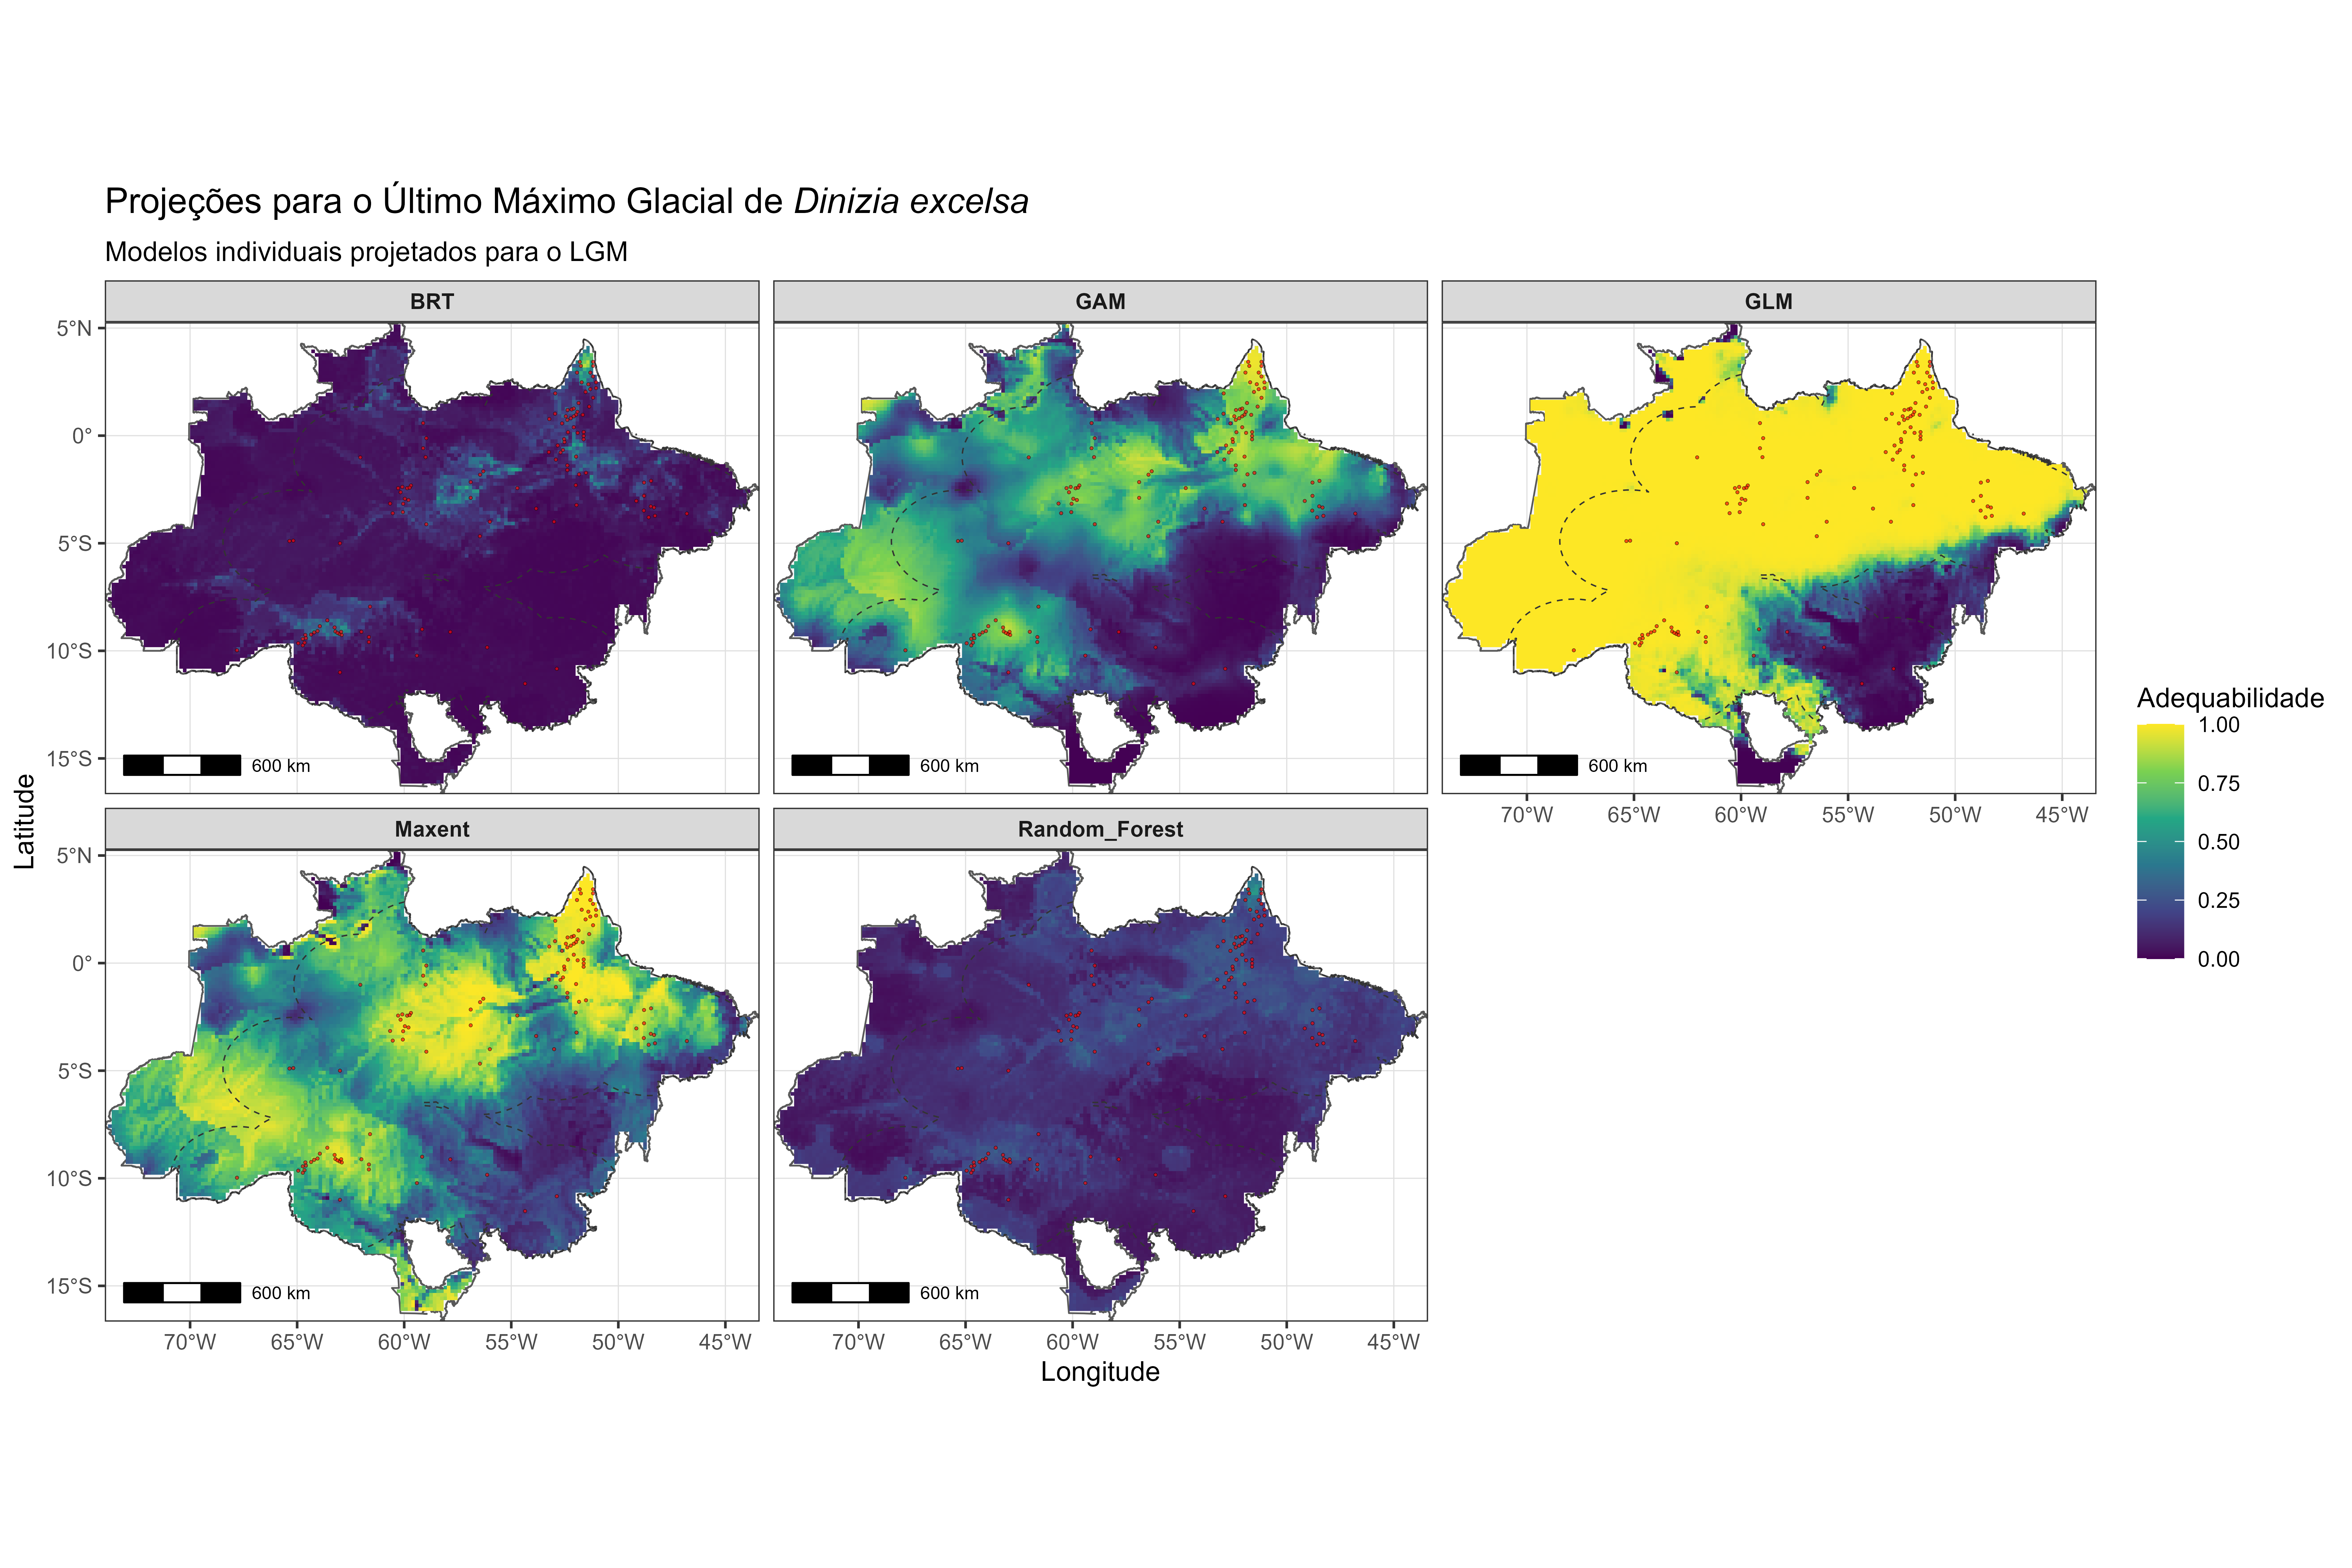
\includegraphics[width=0.98\textwidth]{figuras/unidade15/unidade15_modelos_passado_lgm.png}
\caption{Individual-model projections for \textit{Dinizia excelsa} during the Last Glacial Maximum.}
\label{fig:unidade15_modelos_lgm}
\end{figure}

\section{Paleoclimate ensembles}

Individual projections are combined into an ensemble for each paleoclimatic period. Agreement among algorithms may increase confidence conditional on their shared inputs, but it does not address uncertainty among paleoclimate GCMs or correct common calibration bias. Algorithmic and climatic-model variation should therefore be summarized separately whenever multiple climate reconstructions are available.

\rscriptfile{scripts/unidade15/04_ensemble_passado.R}

\begin{figure}[H]
\centering
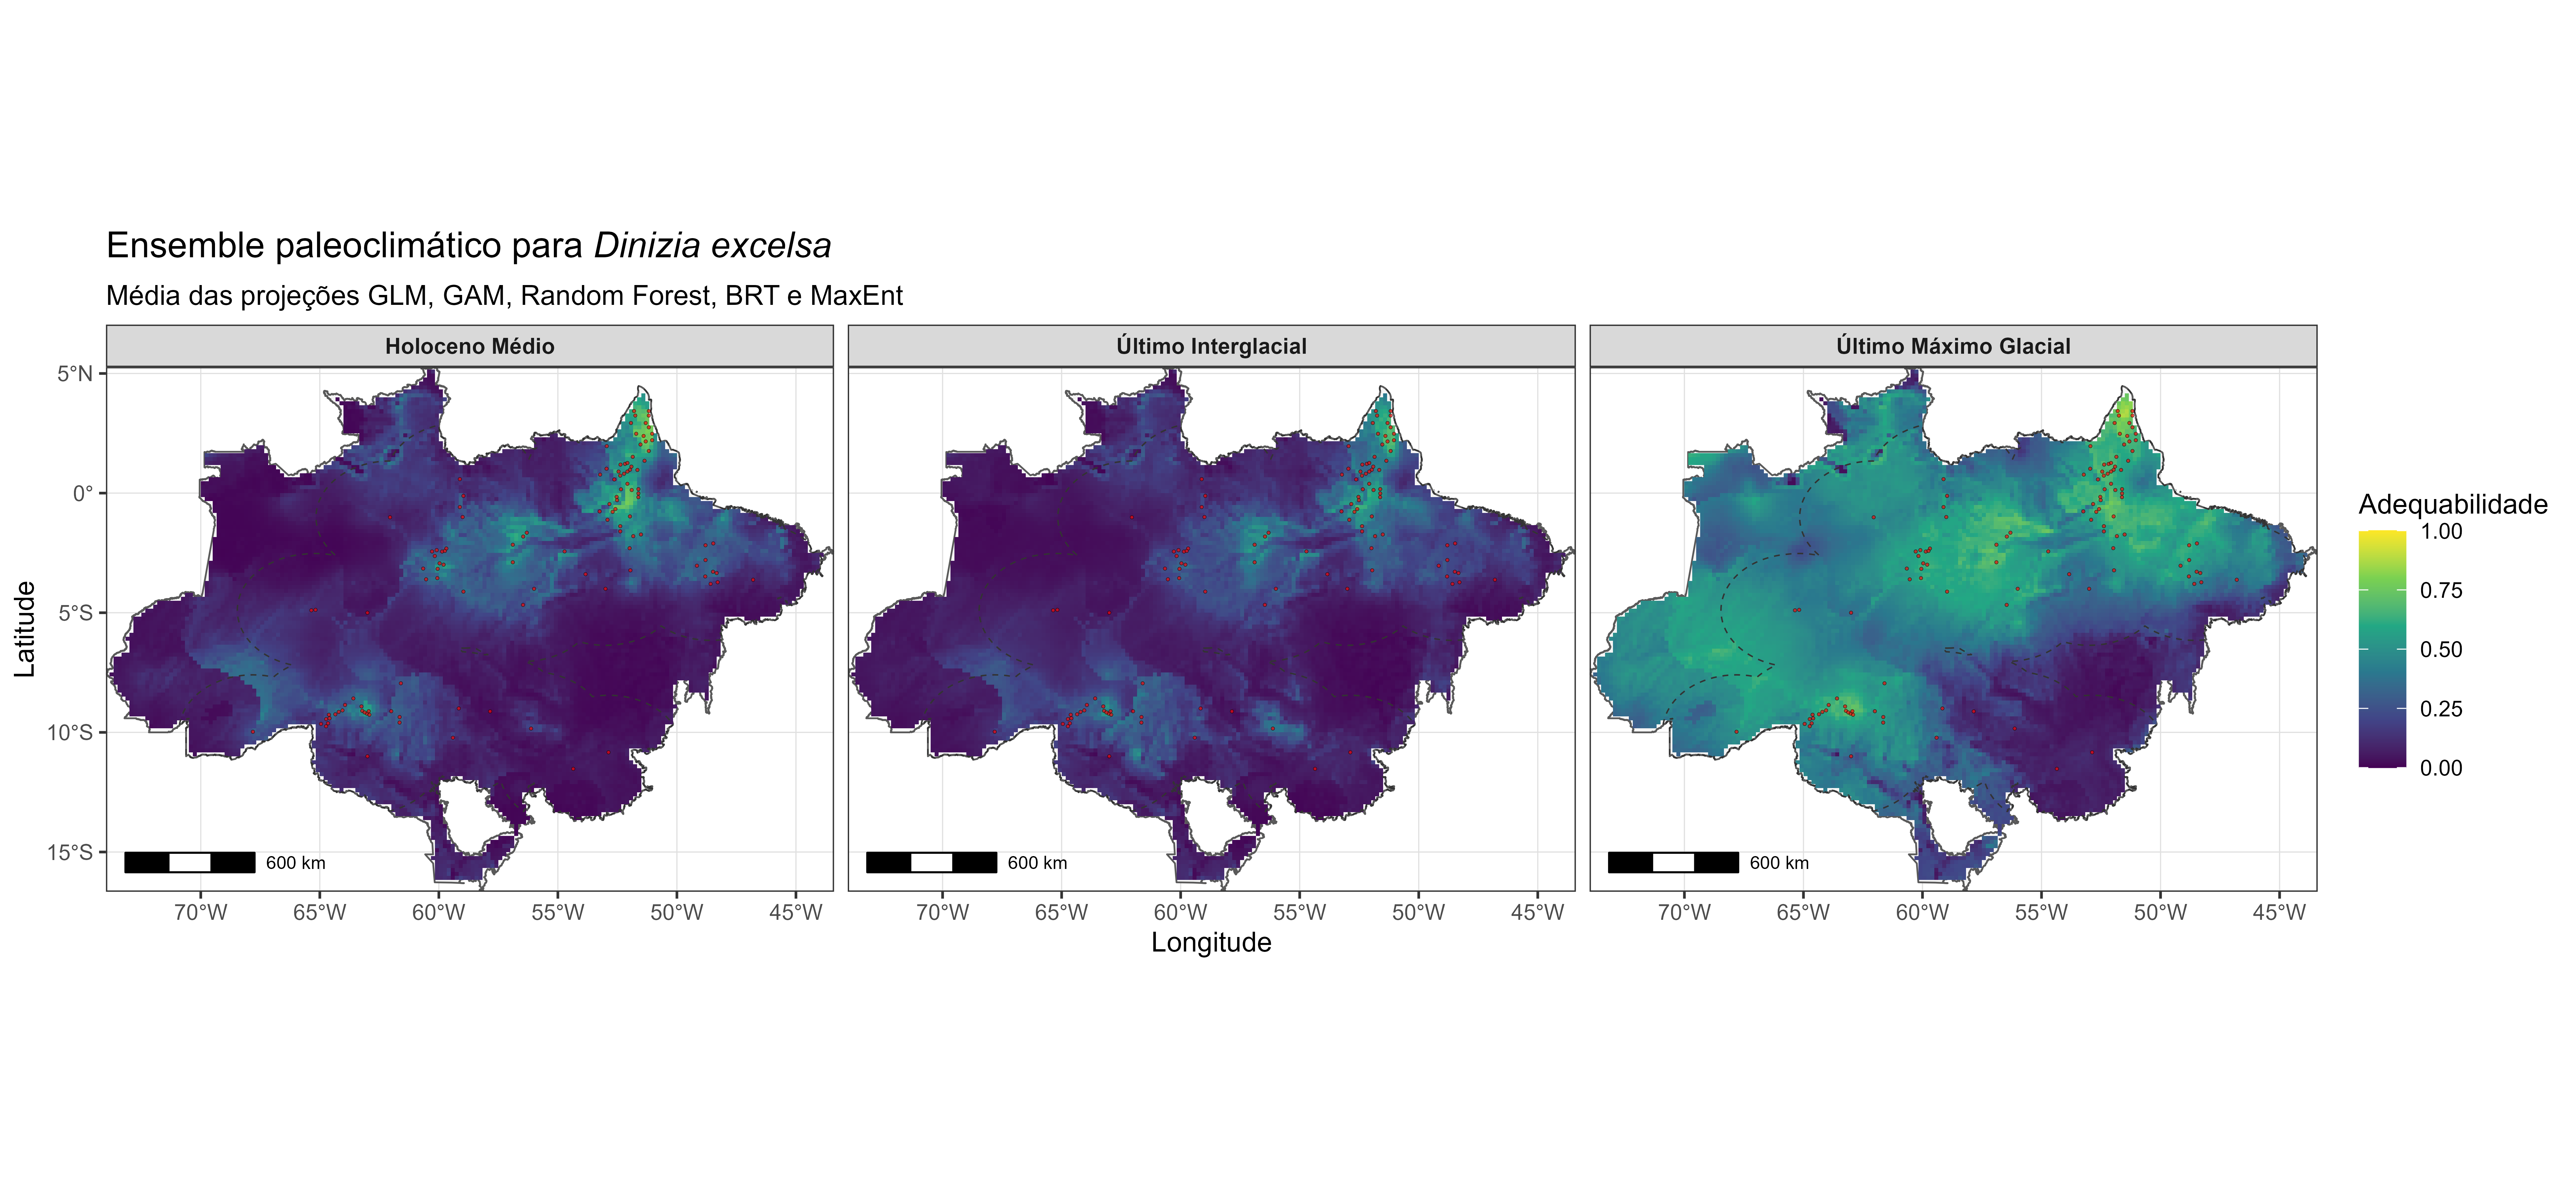
\includegraphics[width=0.96\textwidth]{figuras/unidade15/unidade15_ensemble_passado_periodos.png}
\caption{Paleoclimate ensemble projections of environmental suitability for \textit{Dinizia excelsa}.}
\label{fig:unidade15_ensemble_passado}
\end{figure}

\section{Trajectory through climatic space}

A climatic trajectory compares the contemporary calibration domain with the environmental space available in past periods. Here, an environmental principal component analysis provides a low-dimensional representation of climatic change. The PCA must be fitted to an explicitly defined reference domain and then used to transform other periods with the same centering, scaling, and loadings; fitting a separate PCA to each period would make their axes noncomparable.

\rscriptfile{scripts/unidade15/05_trajetoria_nicho_climatico.R}

\begin{figure}[H]
\centering
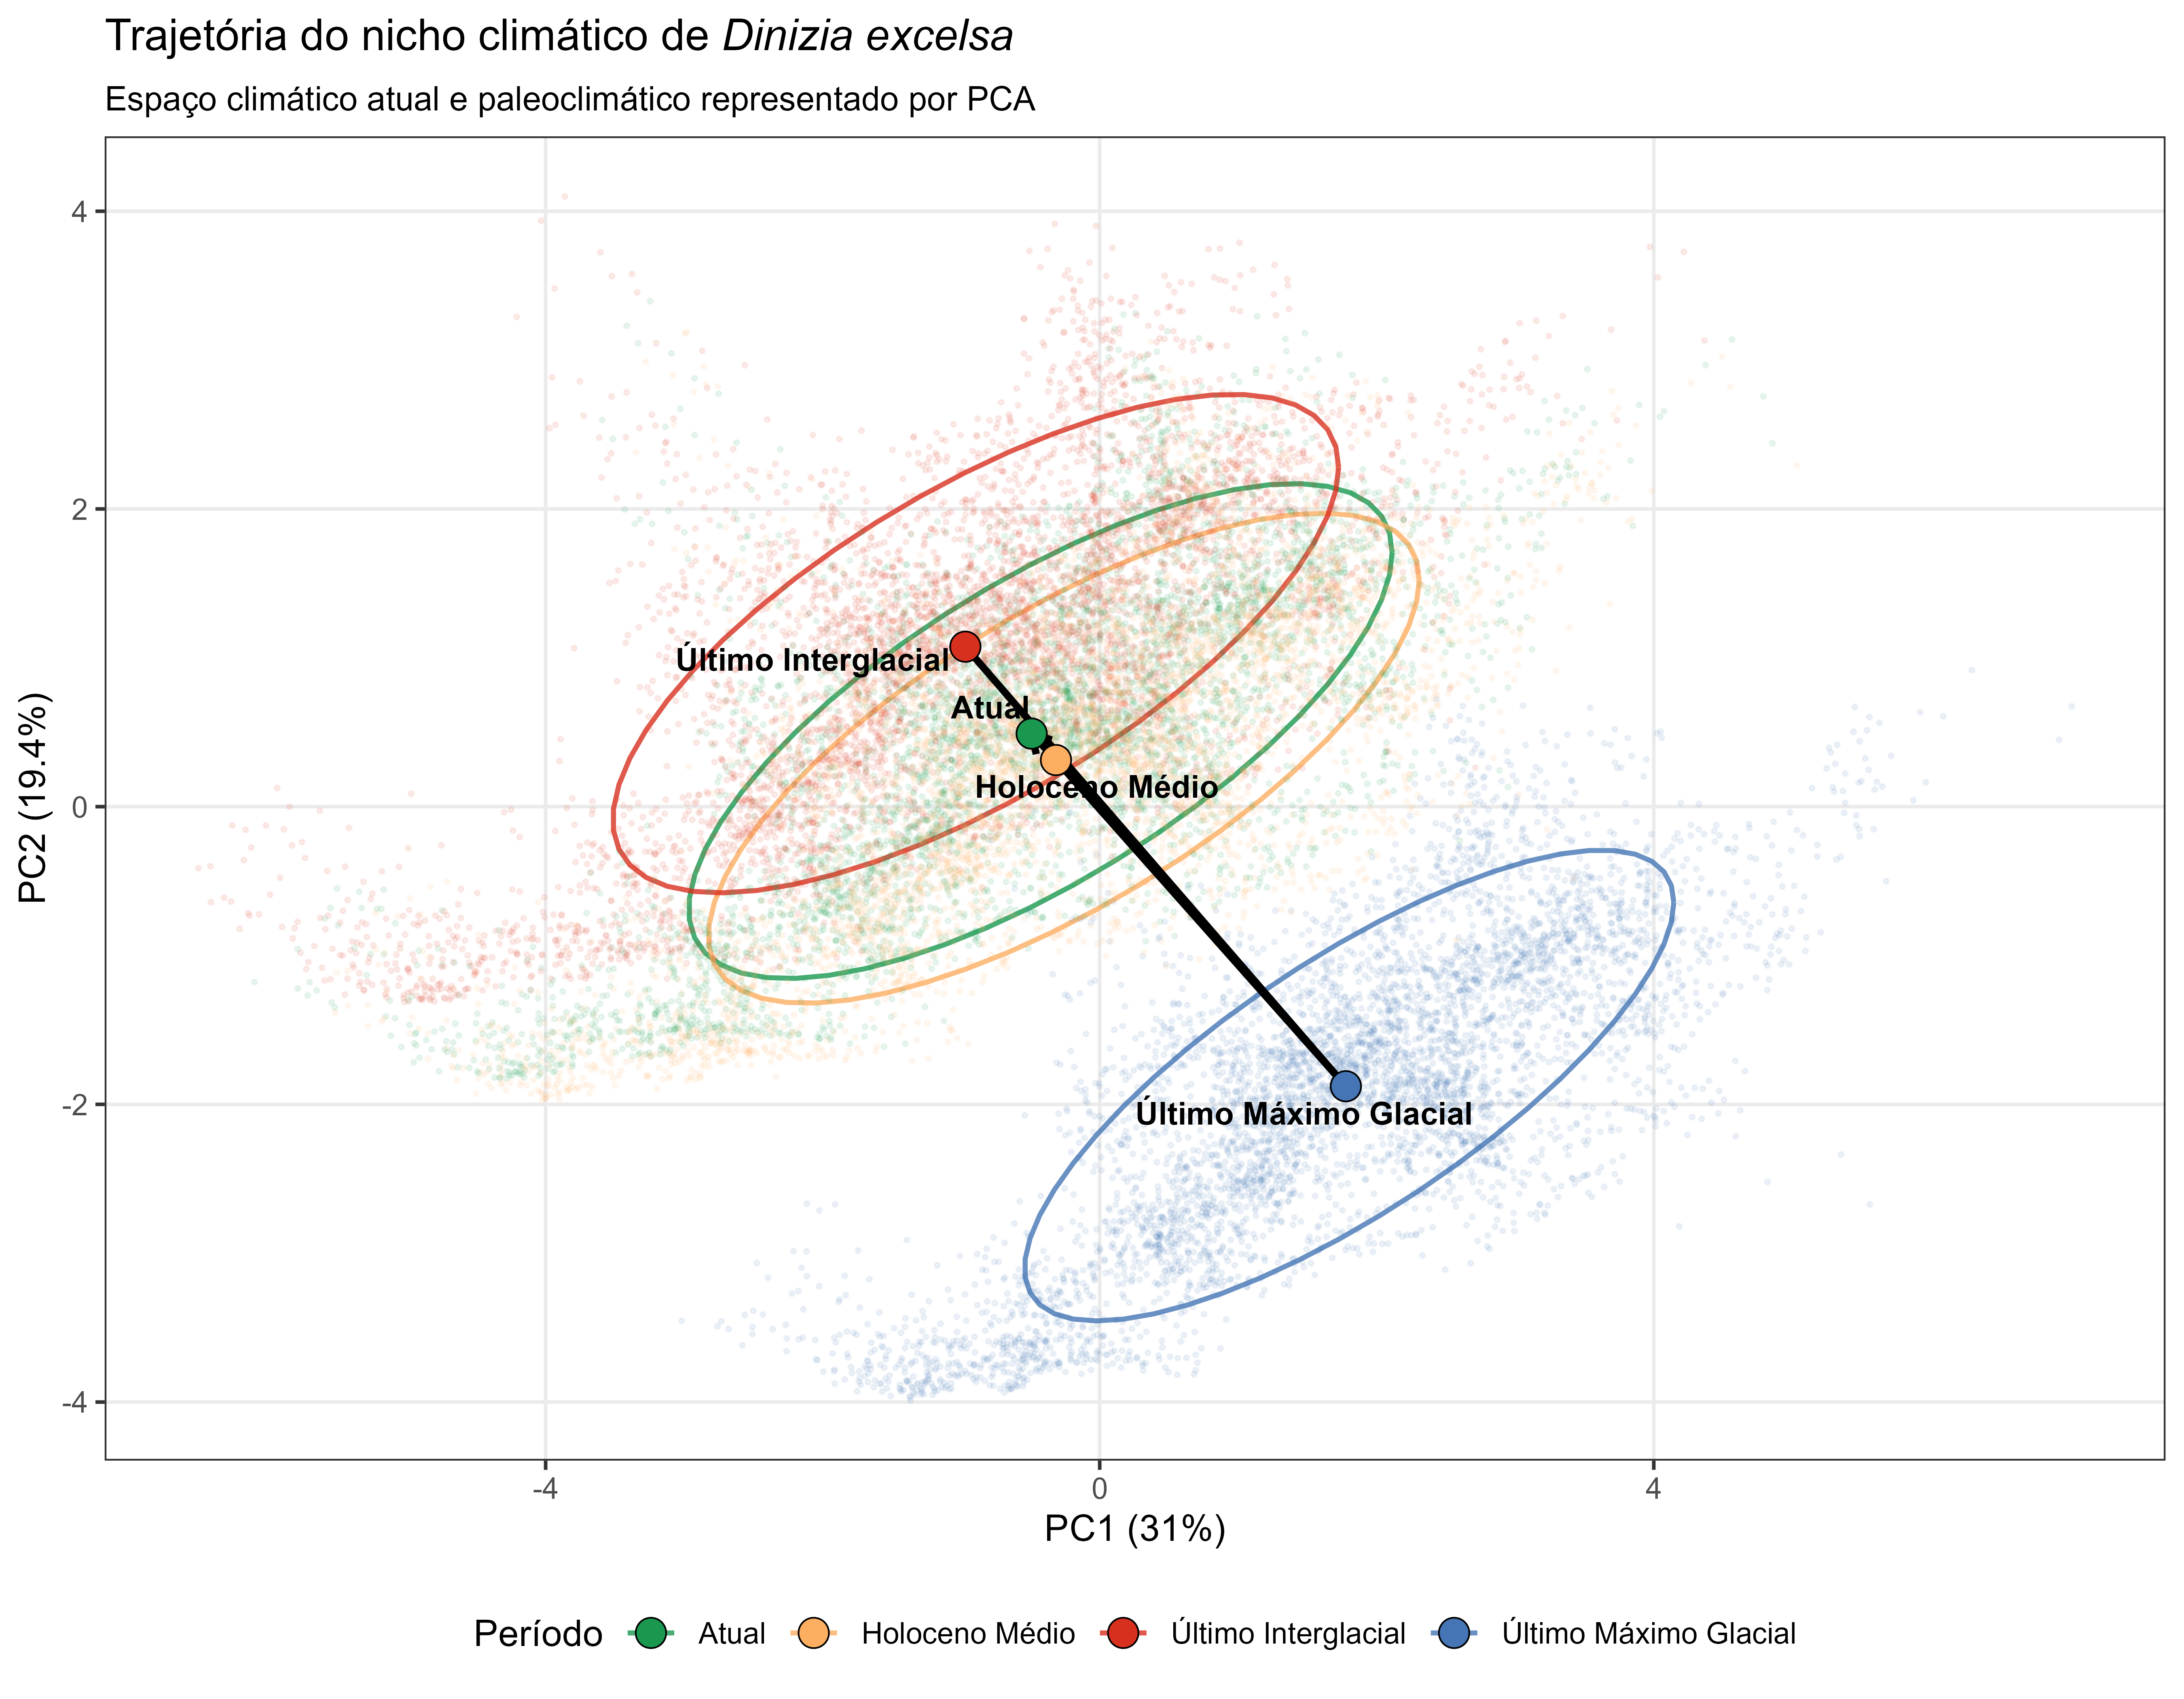
\includegraphics[width=0.88\textwidth]{figuras/unidade15/unidade15_pca_nicho_passado.png}
\caption{Contemporary and paleoclimatic environments for \textit{Dinizia excelsa} represented in a common PCA space.}
\label{fig:unidade15_pca_nicho_passado}
\end{figure}

\section{Historical stability and candidate climatic refugia}

Areas classified as suitable in the baseline and multiple past periods can be interpreted as candidates for long-term climatic stability. They do not prove the existence of refugia or continuous occupation. Threshold choice, temporal resolution, GCM disagreement, sea-level and land-cover changes, dispersal history, and environmental extrapolation all affect the inferred pattern.

\rscriptfile{scripts/unidade15/06_estabilidade_refugios_paleoclimaticos.R}

\begin{figure}[H]
\centering
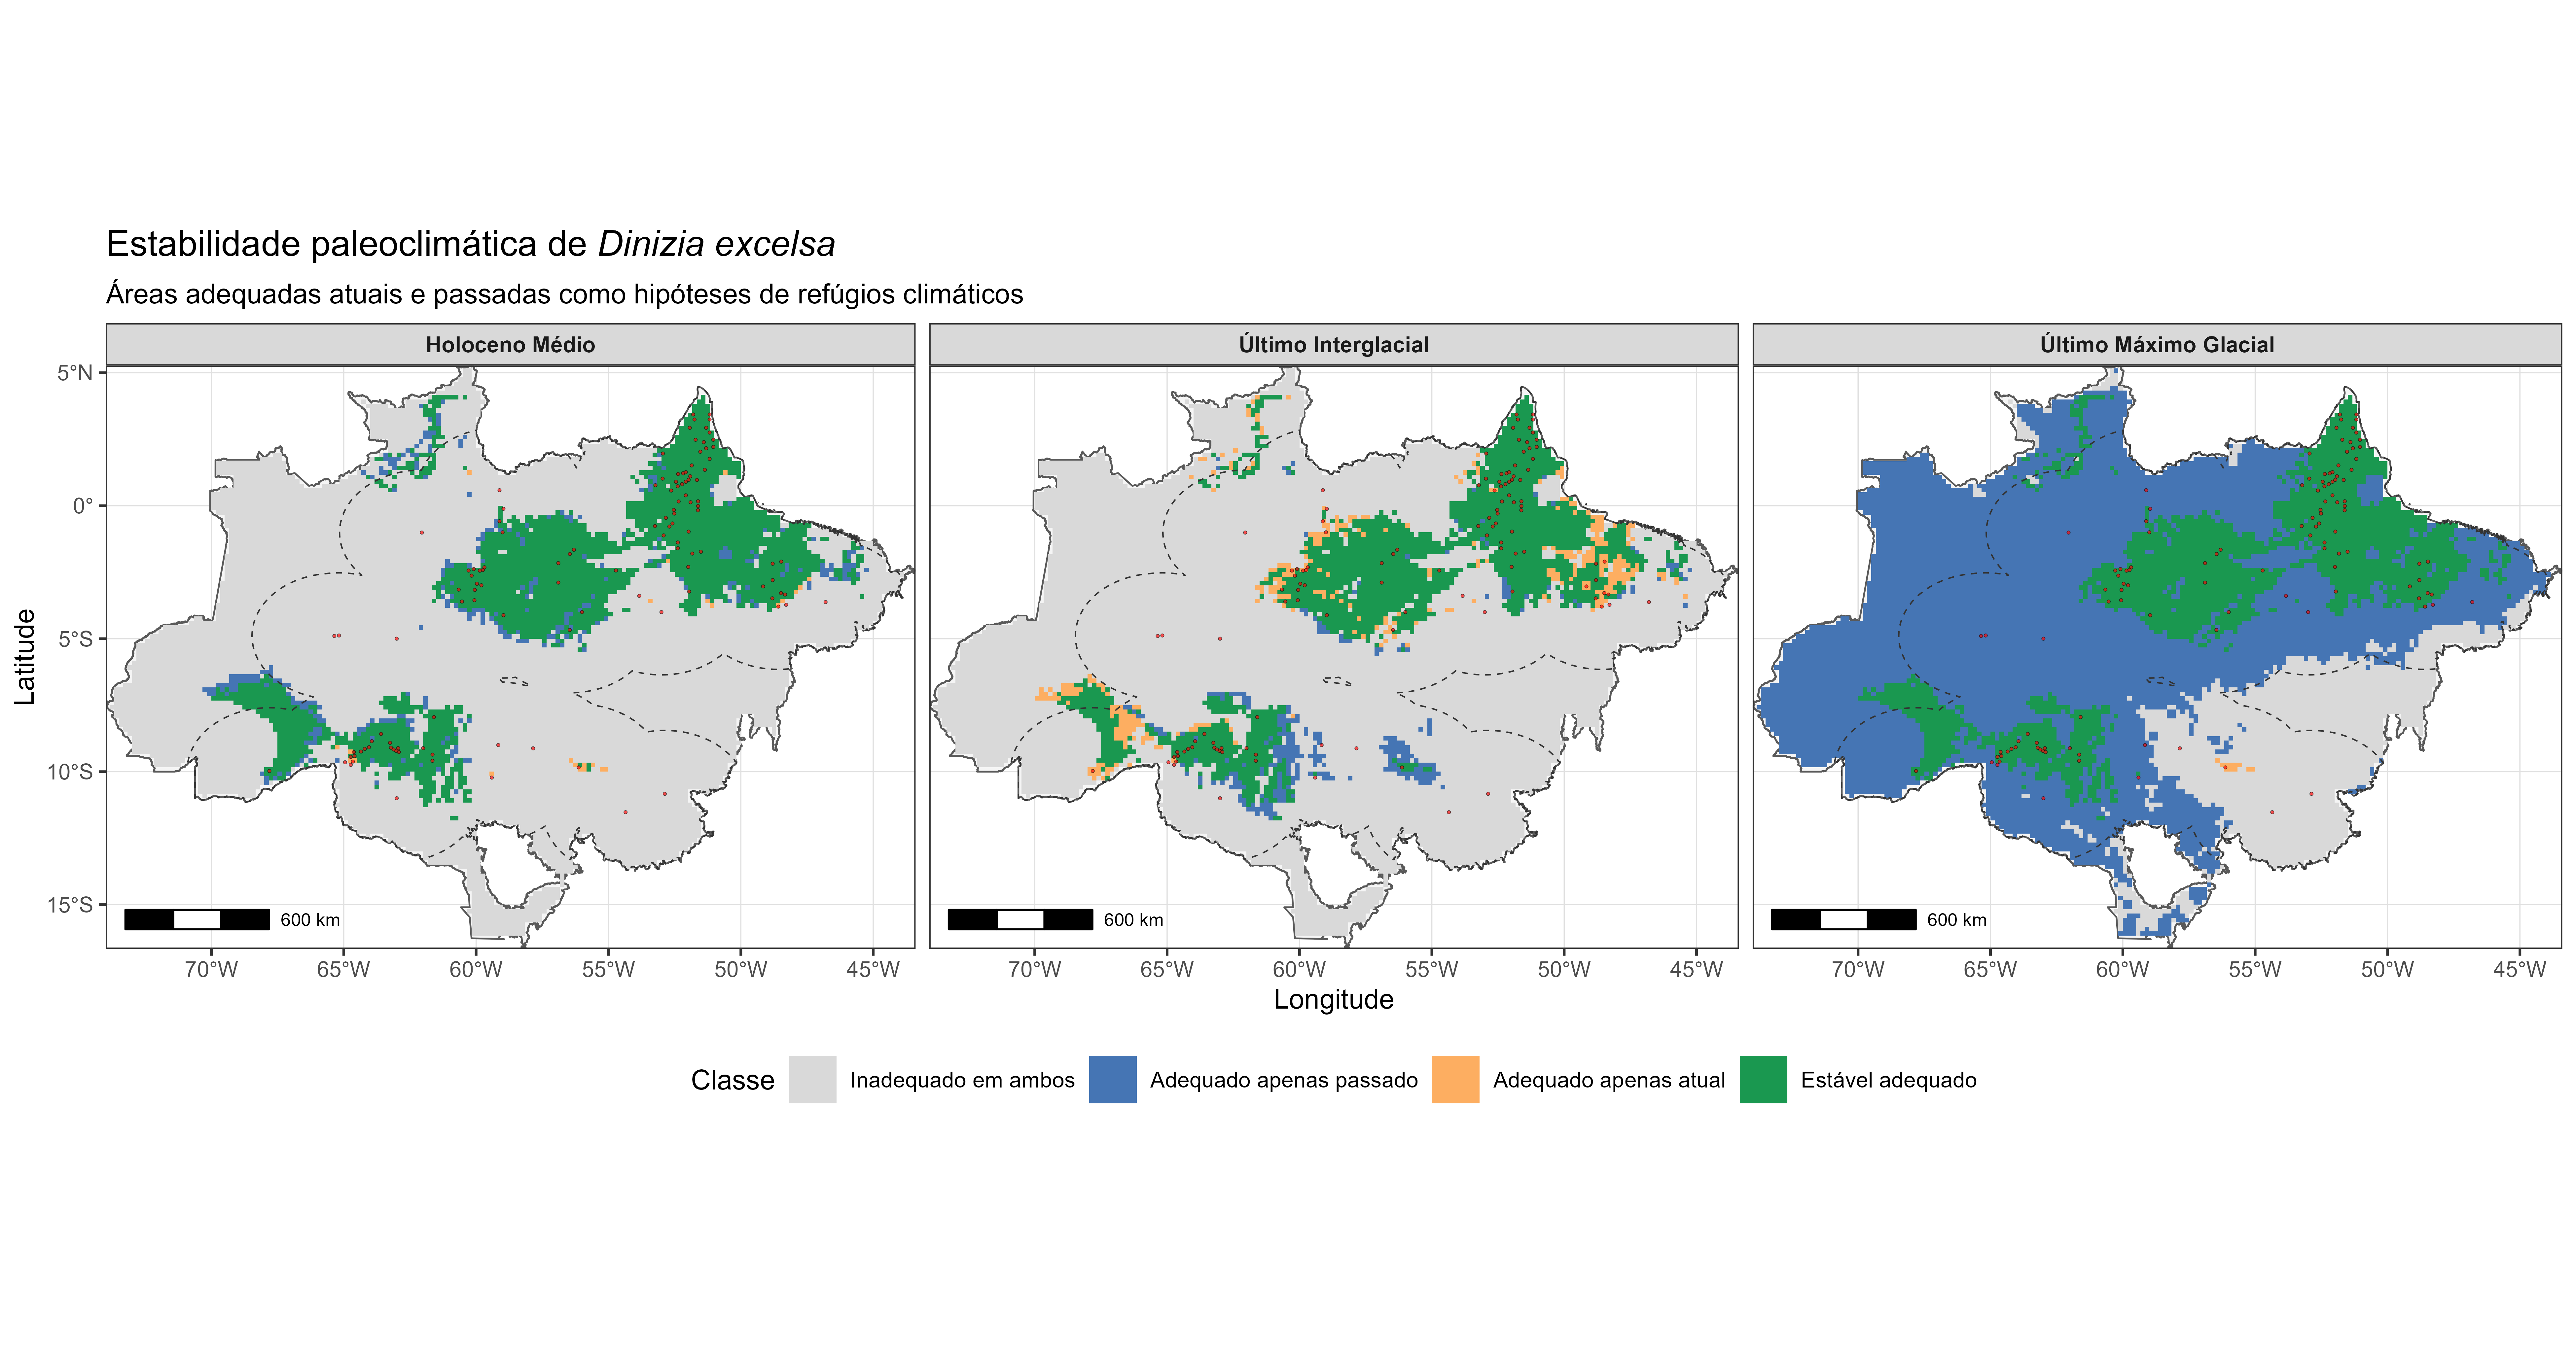
\includegraphics[width=0.96\textwidth]{figuras/unidade15/unidade15_estabilidade_refugios.png}
\caption{Modeled paleoclimatic stability and candidate areas of long-term climatic suitability for \textit{Dinizia excelsa}.}
\label{fig:unidade15_refugios}
\end{figure}

\section{Paleoclimatic synthesis}

\rscriptfile{scripts/unidade15/07_sintese_paleoclimatica.R}

\begin{figure}[H]
\centering
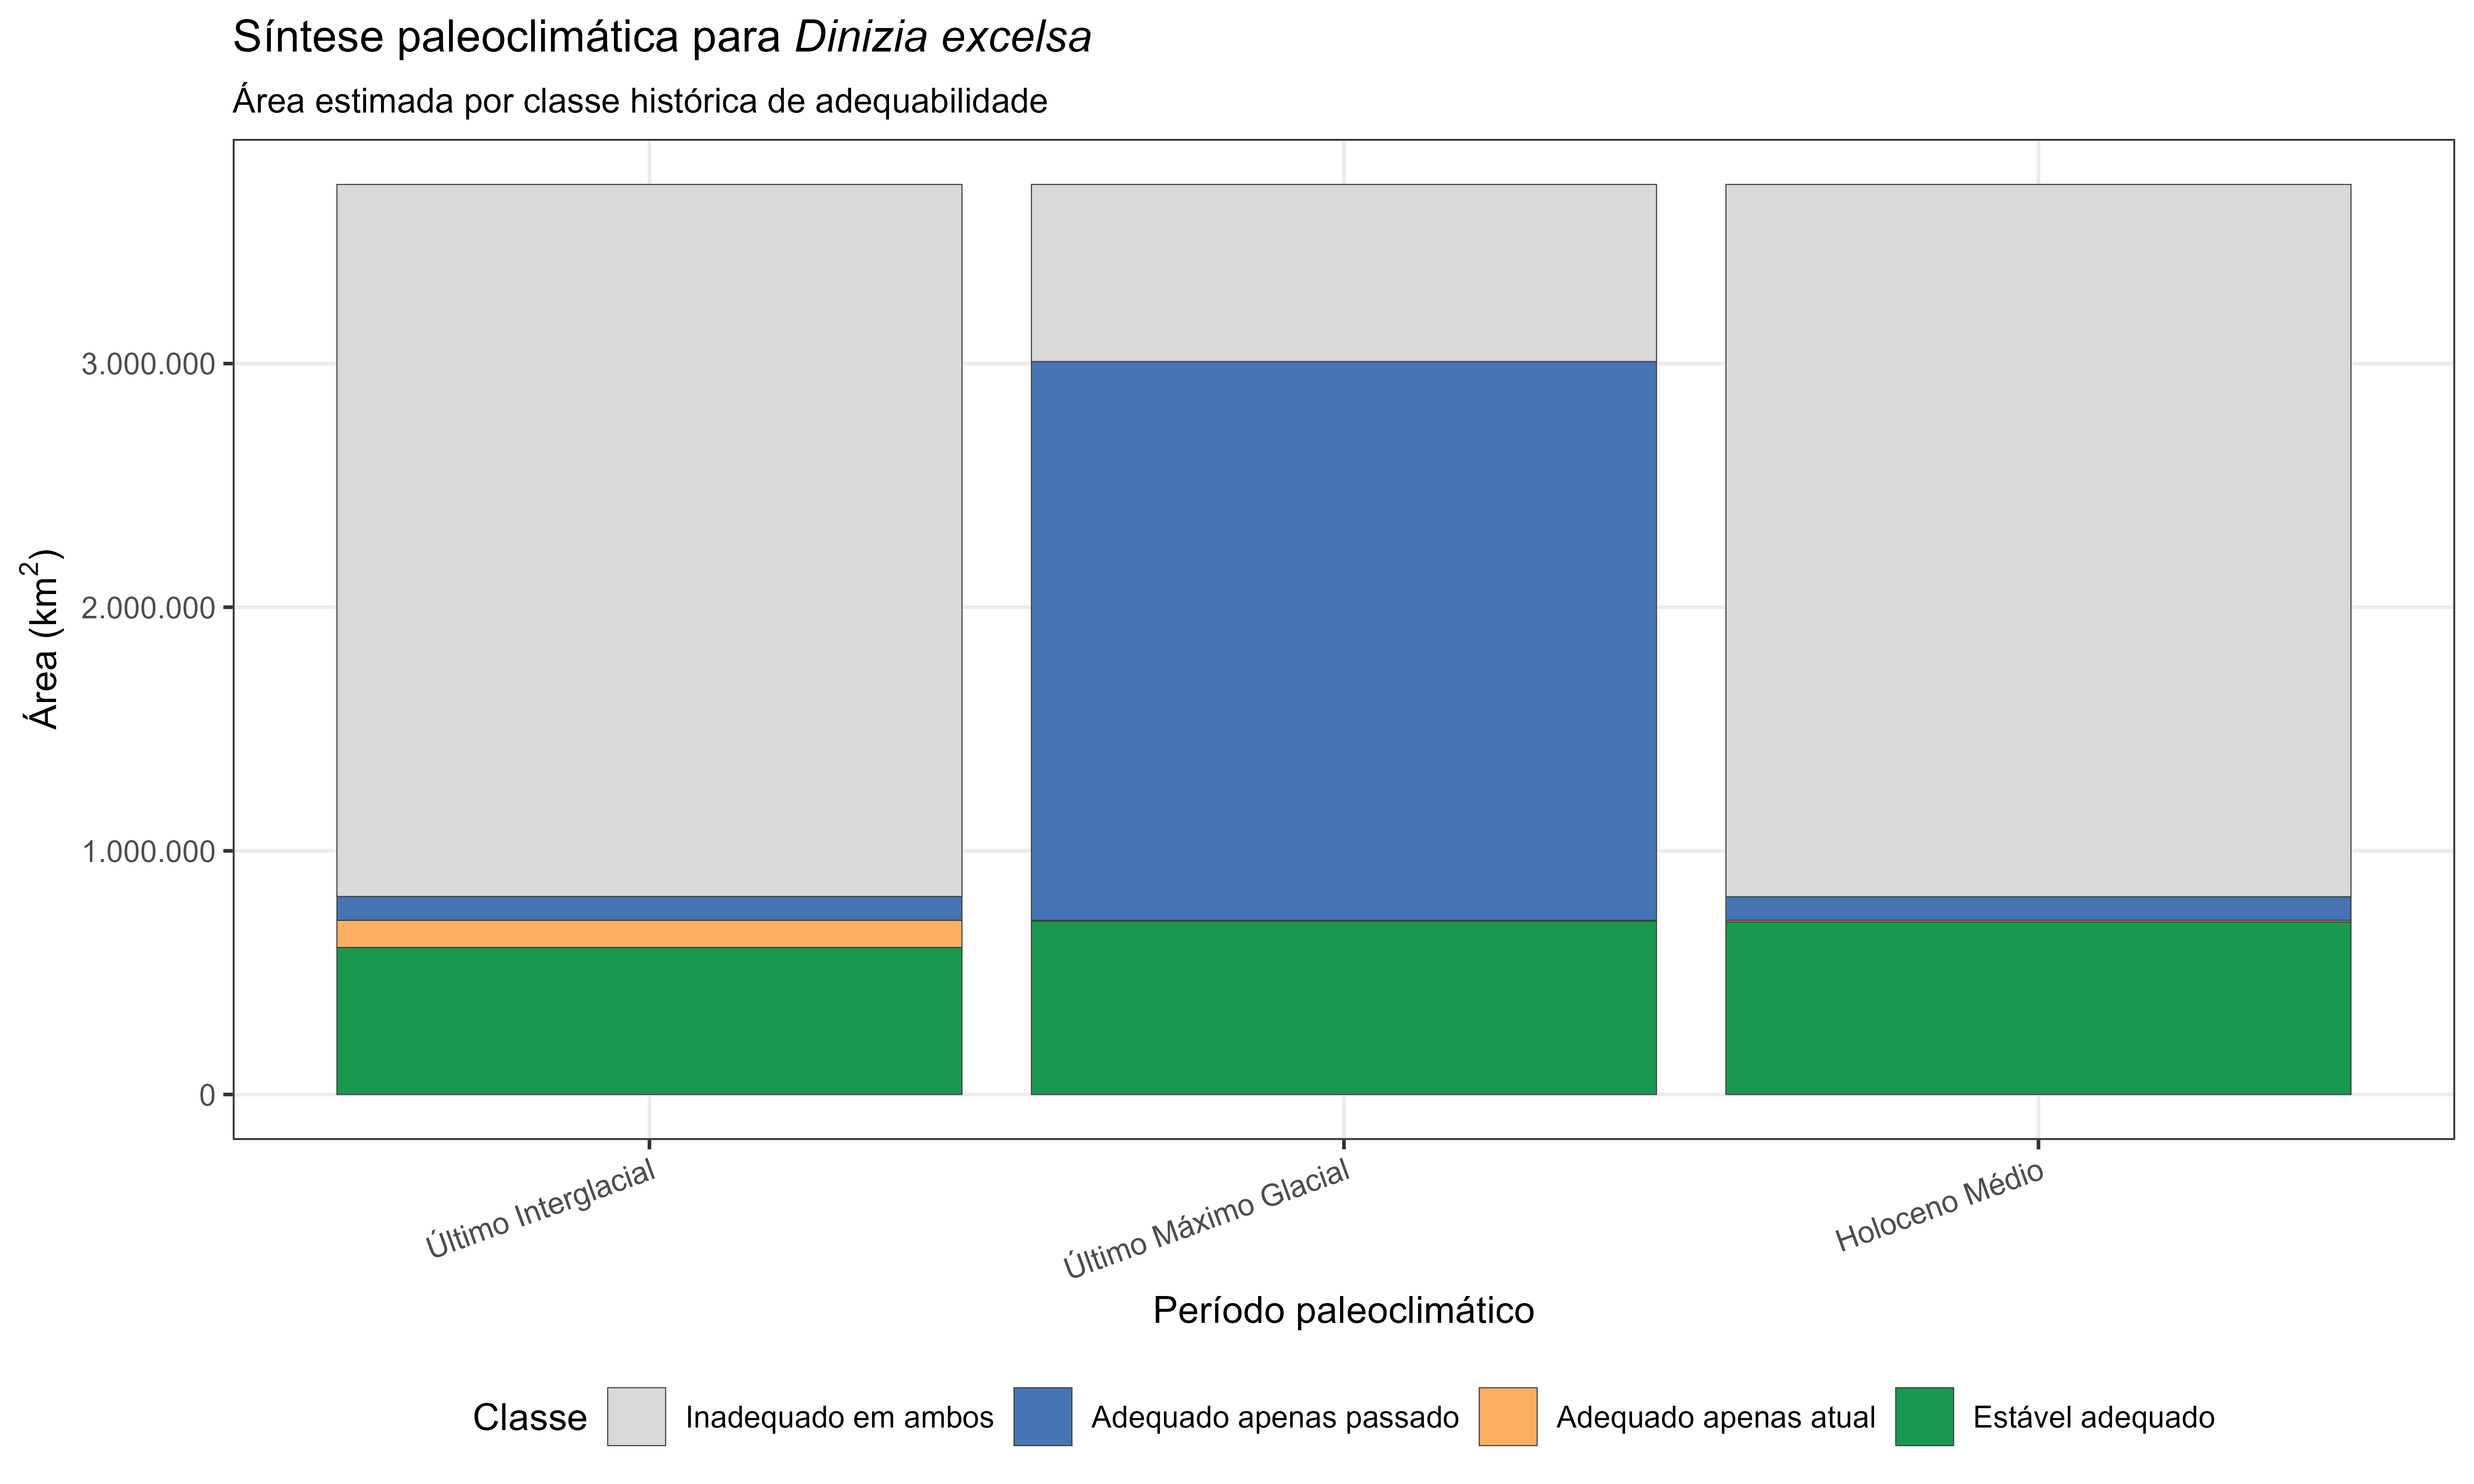
\includegraphics[width=0.88\textwidth]{figuras/unidade15/unidade15_sintese_paleoclimatica.png}
\caption{Estimated suitable area for \textit{Dinizia excelsa} across paleoclimatic periods.}
\label{fig:unidade15_sintese}
\end{figure}

\section{Complete pipeline}

\rscriptfile{scripts/unidade15/08_pipeline_paleoclima.R}

\section{Chapter synthesis}

Paleoclimate reconstruction broadens distribution modeling by connecting contemporary climatic associations with environmental history. For \textit{Dinizia excelsa}, it supports hypotheses about climatic stability, possible areas of historical persistence, and the biogeographic processes underlying its present Amazonian distribution. Strong claims about refugia or past occupancy require independent lines of evidence.

\begin{conceito}[title={\faBook\quad Key message}]
Paleoclimate projections indicate where reconstructed past climates may have been compatible with a species' modeled contemporary climatic association. They do not establish where the species actually occurred.
\end{conceito}

\section{Review exercises}

\begin{enumerate}
\item Distinguish baseline climate, future climate projections, and paleoclimate reconstructions in SDM.
\item What assumptions are made when a contemporary model is projected to the Last Glacial Maximum?
\item Why are temporally stable cells only candidates for climatic refugia?
\item What are the principal sources of uncertainty in paleoclimate SDM projections?
\item How should a common PCA be constructed to compare climatic space across periods?
\item Why is niche conservatism an important, testable assumption in this analysis?
\item Which independent evidence could be combined with paleoclimate projections to inform conservation of Amazonian species?
\end{enumerate}


\chapter[Uncertainty in SDM]{Uncertainty in Species Distribution Modeling}

\begin{objetivos}
By the end of this chapter, readers should be able to identify major sources of uncertainty in SDM; distinguish uncertainty from variability, model disagreement, environmental novelty, and systematic bias; examine contributions from occurrence data, predictors, calibration design, algorithms, global climate models, scenarios, extrapolation, and spatial scale; map algorithmic disagreement for \textit{Dinizia excelsa}; summarize variation across conditional projections without conflating it with probability; combine heterogeneous indicators transparently; and communicate SDM results critically and reproducibly.
\end{objetivos}

\section{Introduction}

Species distribution models do not produce absolute truths about species distributions. They produce estimates conditional on occurrence records, environmental predictors, the accessible area, sampling design, algorithm, parameterization, evaluation scheme, climate period, and projection scenario. A robust SDM analysis must therefore characterize the limitations and uncertainties relevant to its intended inference \parencite{guisan2017habitat,franklin2023,zurell2020benchmarking,yates2018transferability}.

For \textit{Dinizia excelsa}, this task is particularly important because the workflow combines potentially biased records of a large Amazonian tree, several correlative algorithms, climate surfaces, future projections, paleoclimate reconstructions, and temporal extrapolation. Agreement among outputs cannot repair a bias shared by all of these inputs.

\begin{conceito}[title={\faBook\quad Uncertainty in SDM}]
Uncertainty is incomplete knowledge about an estimate, process, or outcome. It may be represented by a probability distribution, interval, sensitivity analysis, disagreement surface, or qualitative limitation. Variability is observed or modeled heterogeneity; bias is systematic deviation; and environmental novelty measures departure from the calibration domain. These concepts are related but not interchangeable.
\end{conceito}

\section{An uncertainty taxonomy}

Useful categories include:

\begin{itemize}
\item \textbf{occurrence uncertainty}: identification errors, coordinate errors, temporal mismatch, imperfect detection, sampling bias, and limited sample size;
\item \textbf{predictor uncertainty}: measurement and interpolation error, product disagreement, scale mismatch, collinearity, and omission of relevant drivers;
\item \textbf{design uncertainty}: choices about the accessible area, background, thinning, folds, prevalence, and evaluation data;
\item \textbf{model uncertainty}: algorithm, feature representation, parameter values, tuning criterion, random seed, and fitted coefficients;
\item \textbf{projection uncertainty}: GCM, downscaling product, emissions pathway, time horizon, and paleoclimate reconstruction;
\item \textbf{transfer uncertainty}: environmental novelty, clamping, nonstationary relationships, dispersal, biotic interactions, and land-use change;
\item \textbf{decision uncertainty}: threshold, weighting, aggregation, utility, and the consequences assigned to false positives and false negatives.
\end{itemize}

Some components are reducible through better data or design; others reflect genuine variation among plausible futures or structural assumptions. A single map rarely captures them all.

\begin{atencao}[title={\faExclamationTriangle\quad Uncertainty is not disposable error}]
Uncertainty should not be hidden or treated as a defect that an ensemble automatically removes. It indicates where conclusions are stable, where they depend on analytical choices, and where additional evidence would be most valuable.
\end{atencao}

\section{Algorithmic disagreement}

Algorithmic disagreement describes variation among predictions from different modeling approaches. In this workflow, it is summarized by the cellwise standard deviation across GLM, GAM, Random Forest, BRT, and Maxent predictions.

\rscriptfile{scripts/unidade16/01_estrutura_pastas.R}

\rscriptfile{scripts/unidade16/02_incerteza_algoritmica_atual.R}

\begin{figure}[H]
\centering
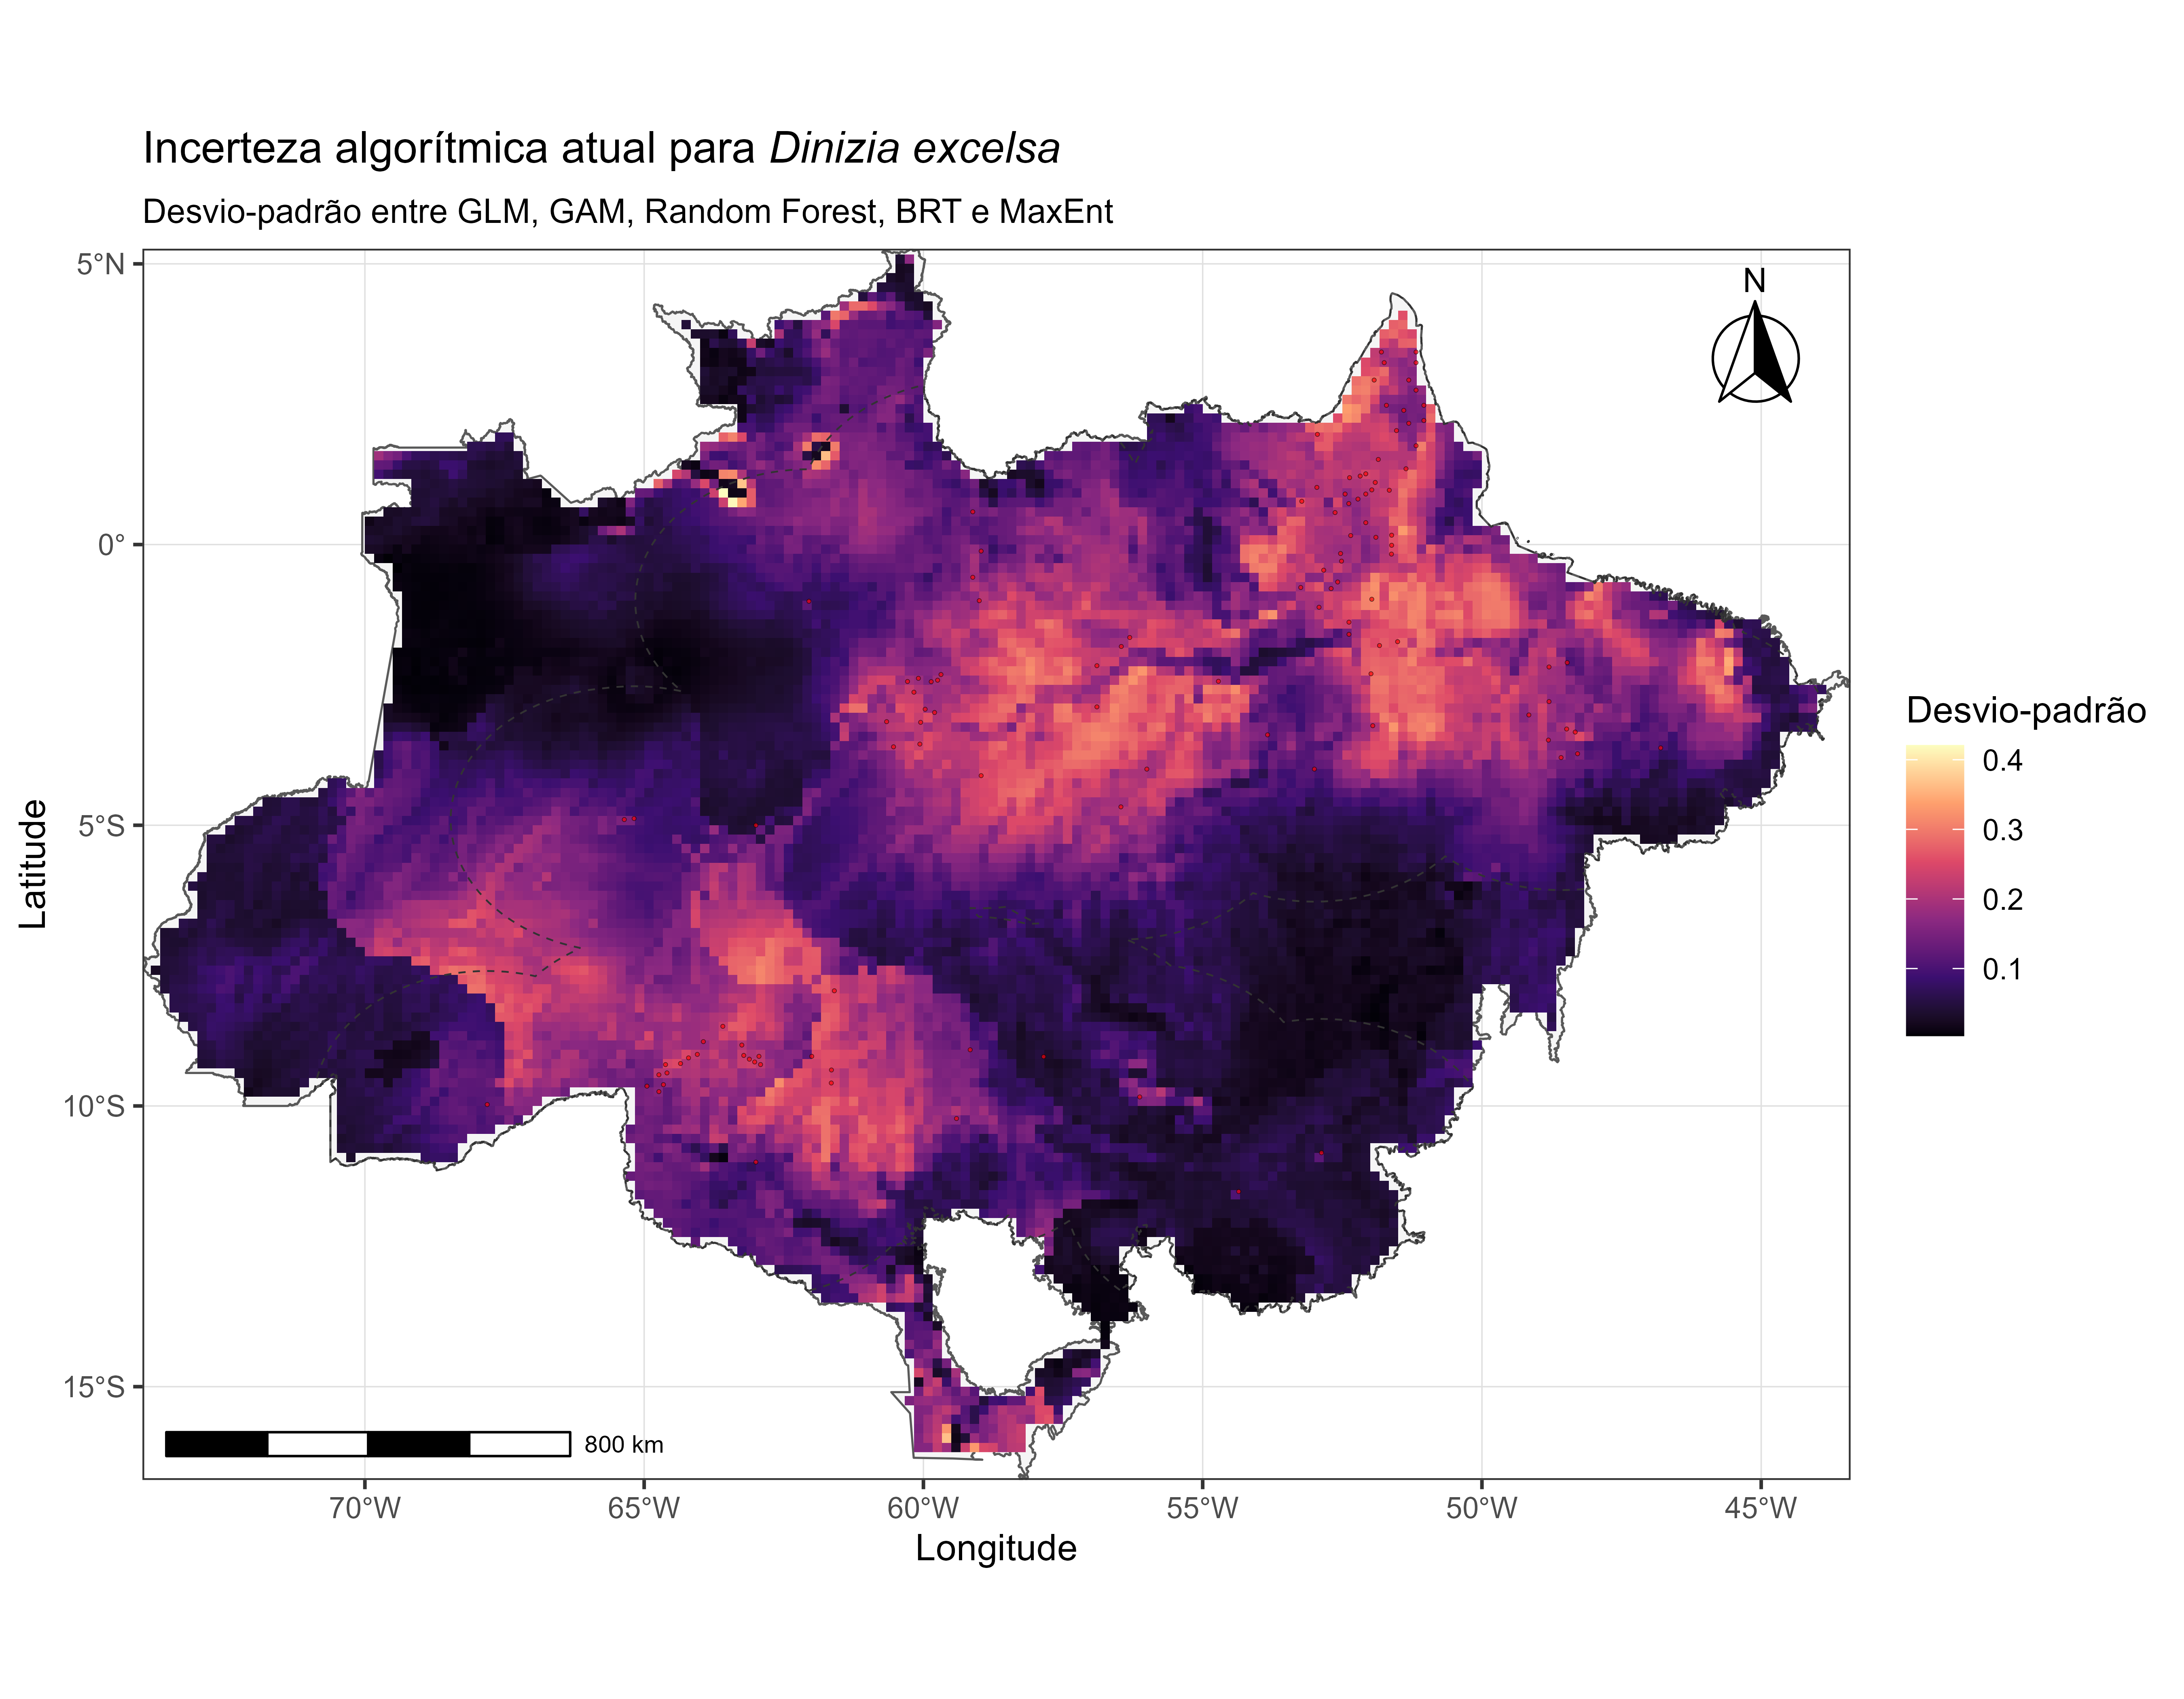
\includegraphics[width=0.88\textwidth]{figuras/unidade16/unidade16_incerteza_algoritmica_atual.png}
\caption{Contemporary algorithmic disagreement for \textit{Dinizia excelsa}, summarized by the standard deviation of predictions from GLM, GAM, Random Forest, BRT, and Maxent.}
\label{fig:unidade16_incerteza_algoritmica}
\end{figure}

This standard deviation is descriptive, not a confidence interval. Its interpretation is valid only when model outputs are on a sufficiently comparable scale. It also combines differences in algorithms with any differences in data subsets, tuning, or calibration procedures. To isolate algorithmic effects, keep other workflow components fixed and retain replicate or fold identifiers.

\section{Variation across future scenarios}

The spread among SSP1--2.6, SSP2--4.5, SSP3--7.0, and SSP5--8.5 projections describes sensitivity to alternative socioeconomic and forcing pathways. Because the pathways are conditional scenarios rather than random samples from a probability distribution, their standard deviation should not be interpreted as a probabilistic confidence measure.

\rscriptfile{scripts/unidade16/03_incerteza_cenarios_futuros.R}

\begin{figure}[H]
\centering
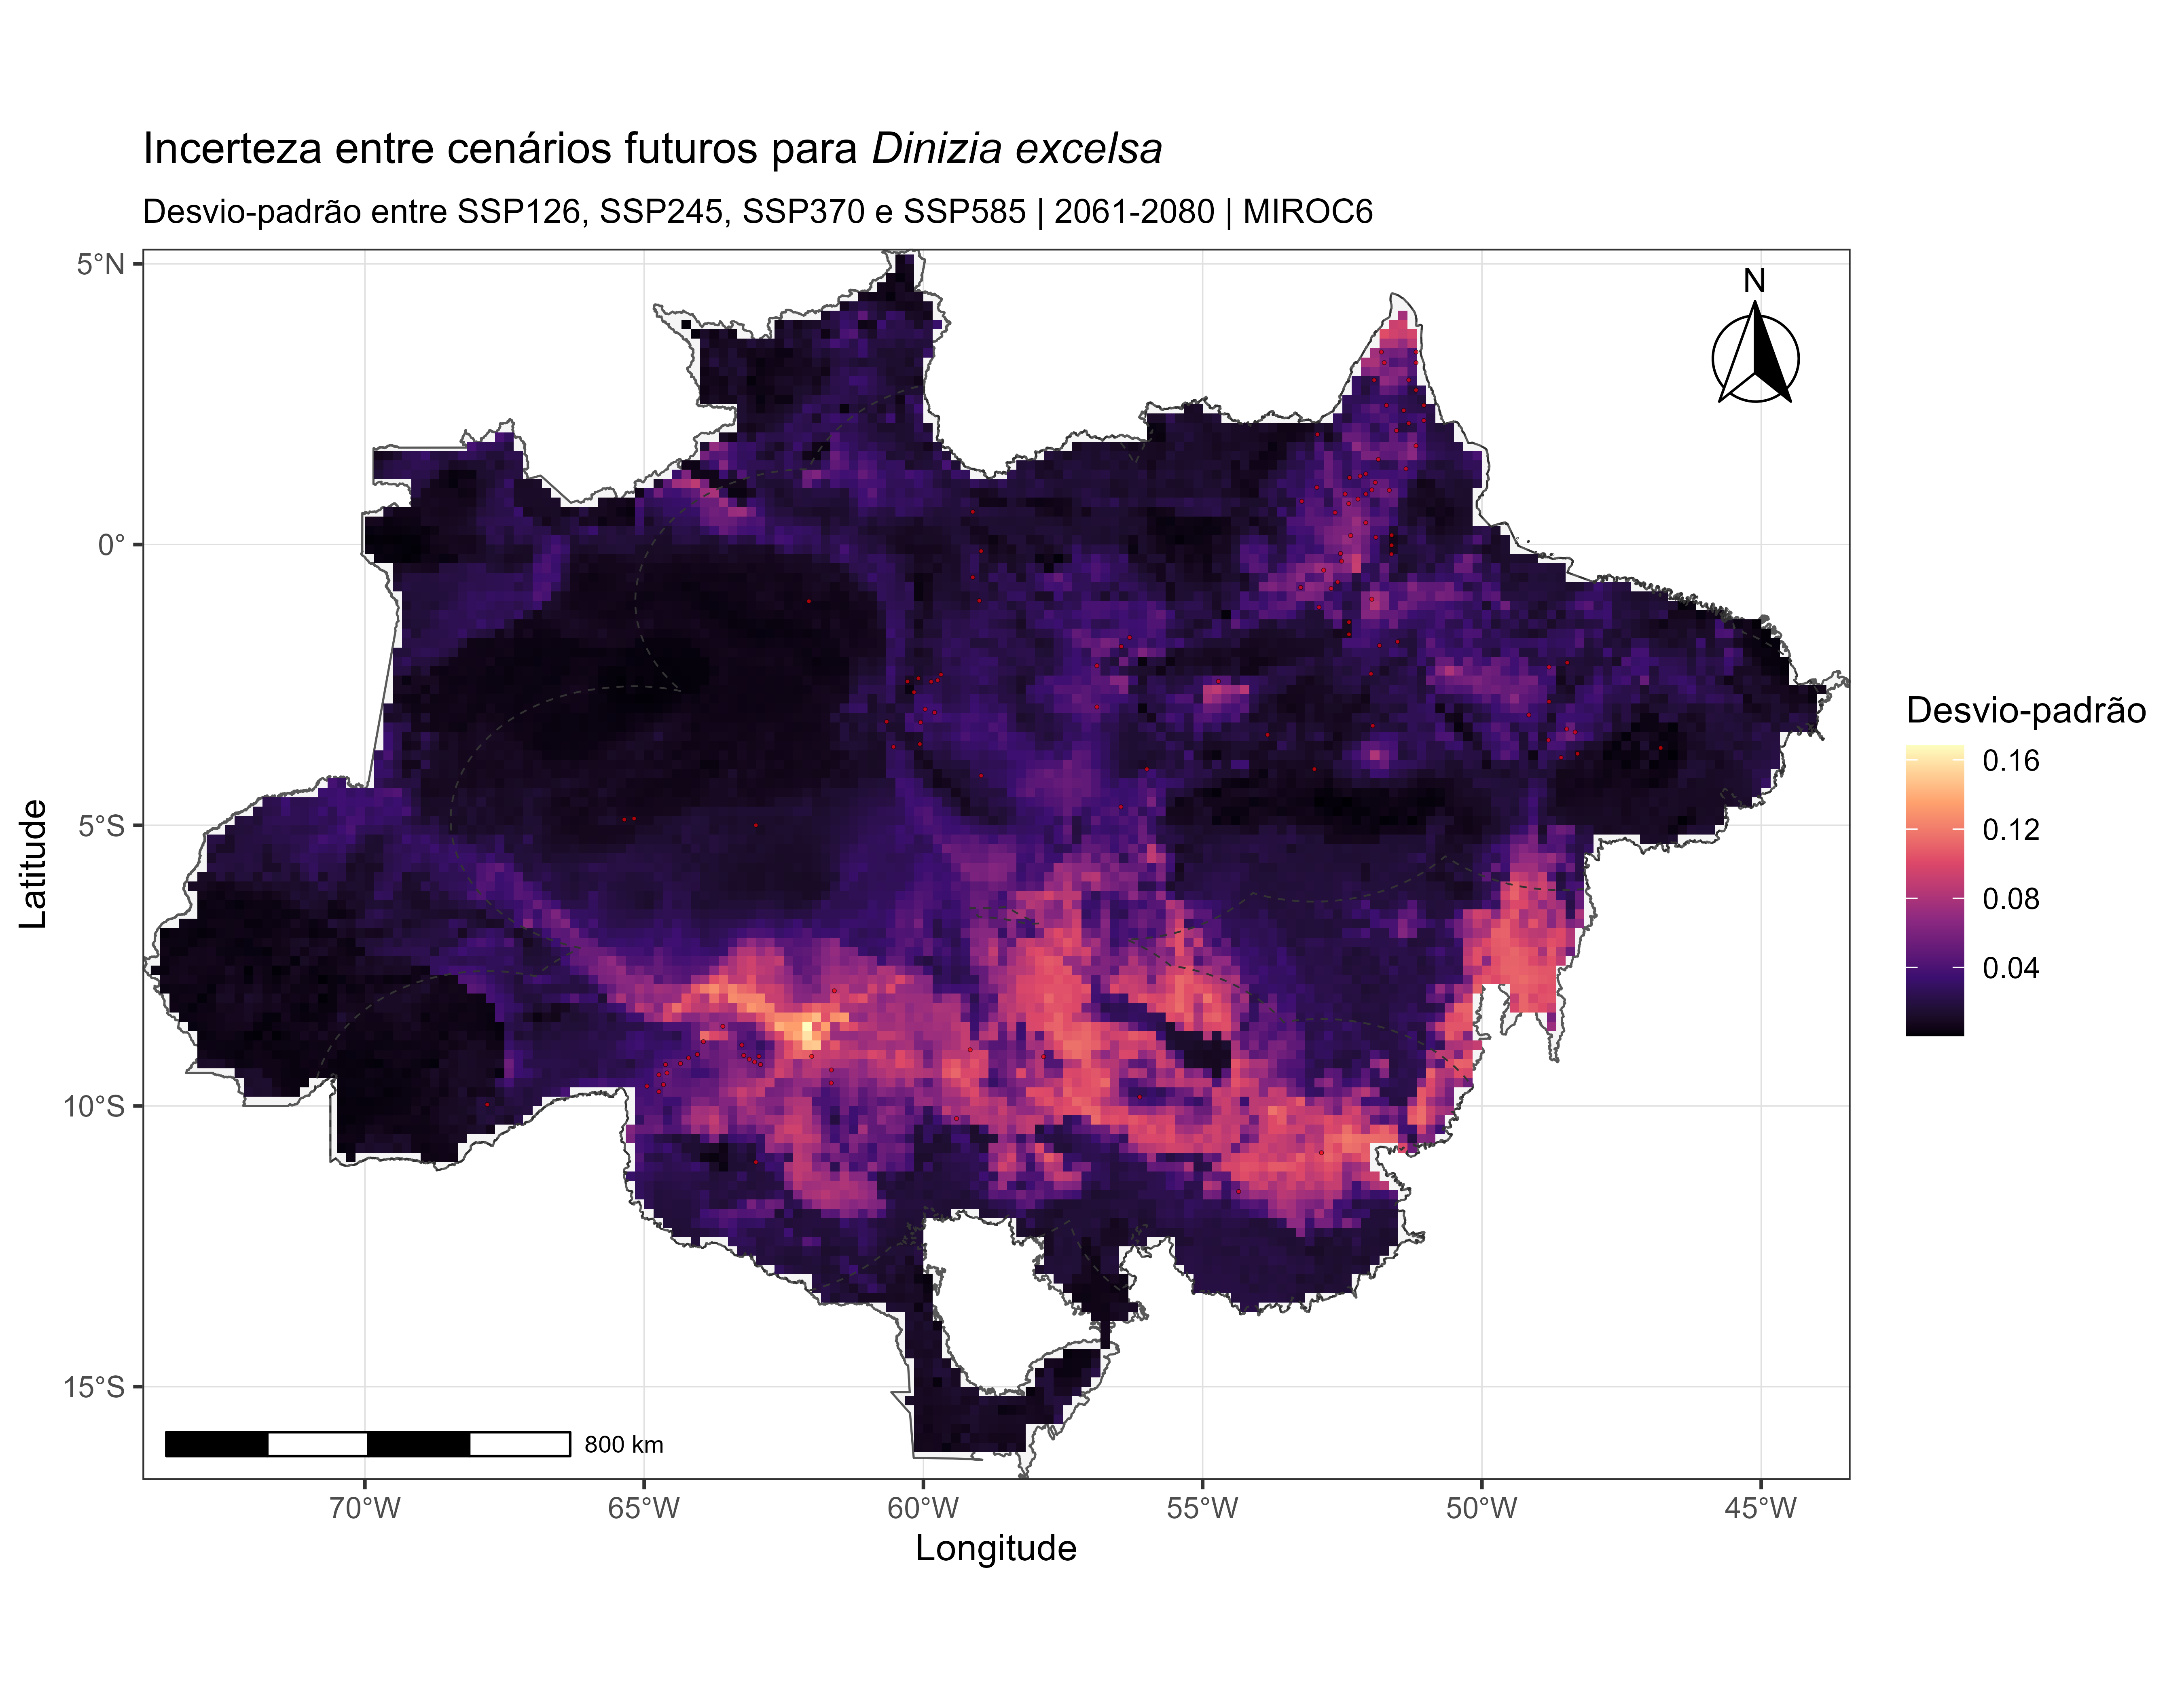
\includegraphics[width=0.88\textwidth]{figuras/unidade16/unidade16_incerteza_cenarios_futuros.png}
\caption{Spread among future ensemble projections for \textit{Dinizia excelsa} under SSP1--2.6, SSP2--4.5, SSP3--7.0, and SSP5--8.5.}
\label{fig:unidade16_incerteza_cenarios}
\end{figure}

A fuller factorial design separates at least algorithm, GCM, SSP, time horizon, and calibration replicate. Variation among GCMs under the same SSP reflects climate-model disagreement, whereas variation among SSPs reflects alternative boundary conditions and increases with the time horizon. Pooling both into one standard deviation obscures their distinct meanings.

\section{Environmental novelty and extrapolation risk}

MESS and MOP identify projection environments that depart from the calibration domain. They do not estimate prediction error directly and should not be treated as posterior uncertainty. Instead, they are diagnostics of support: extrapolative cells rely more strongly on fitted response shapes, clamping rules, and assumptions of temporal or spatial stationarity.

\rscriptfile{scripts/unidade16/04_incerteza_extrapolacao.R}

\begin{figure}[H]
\centering
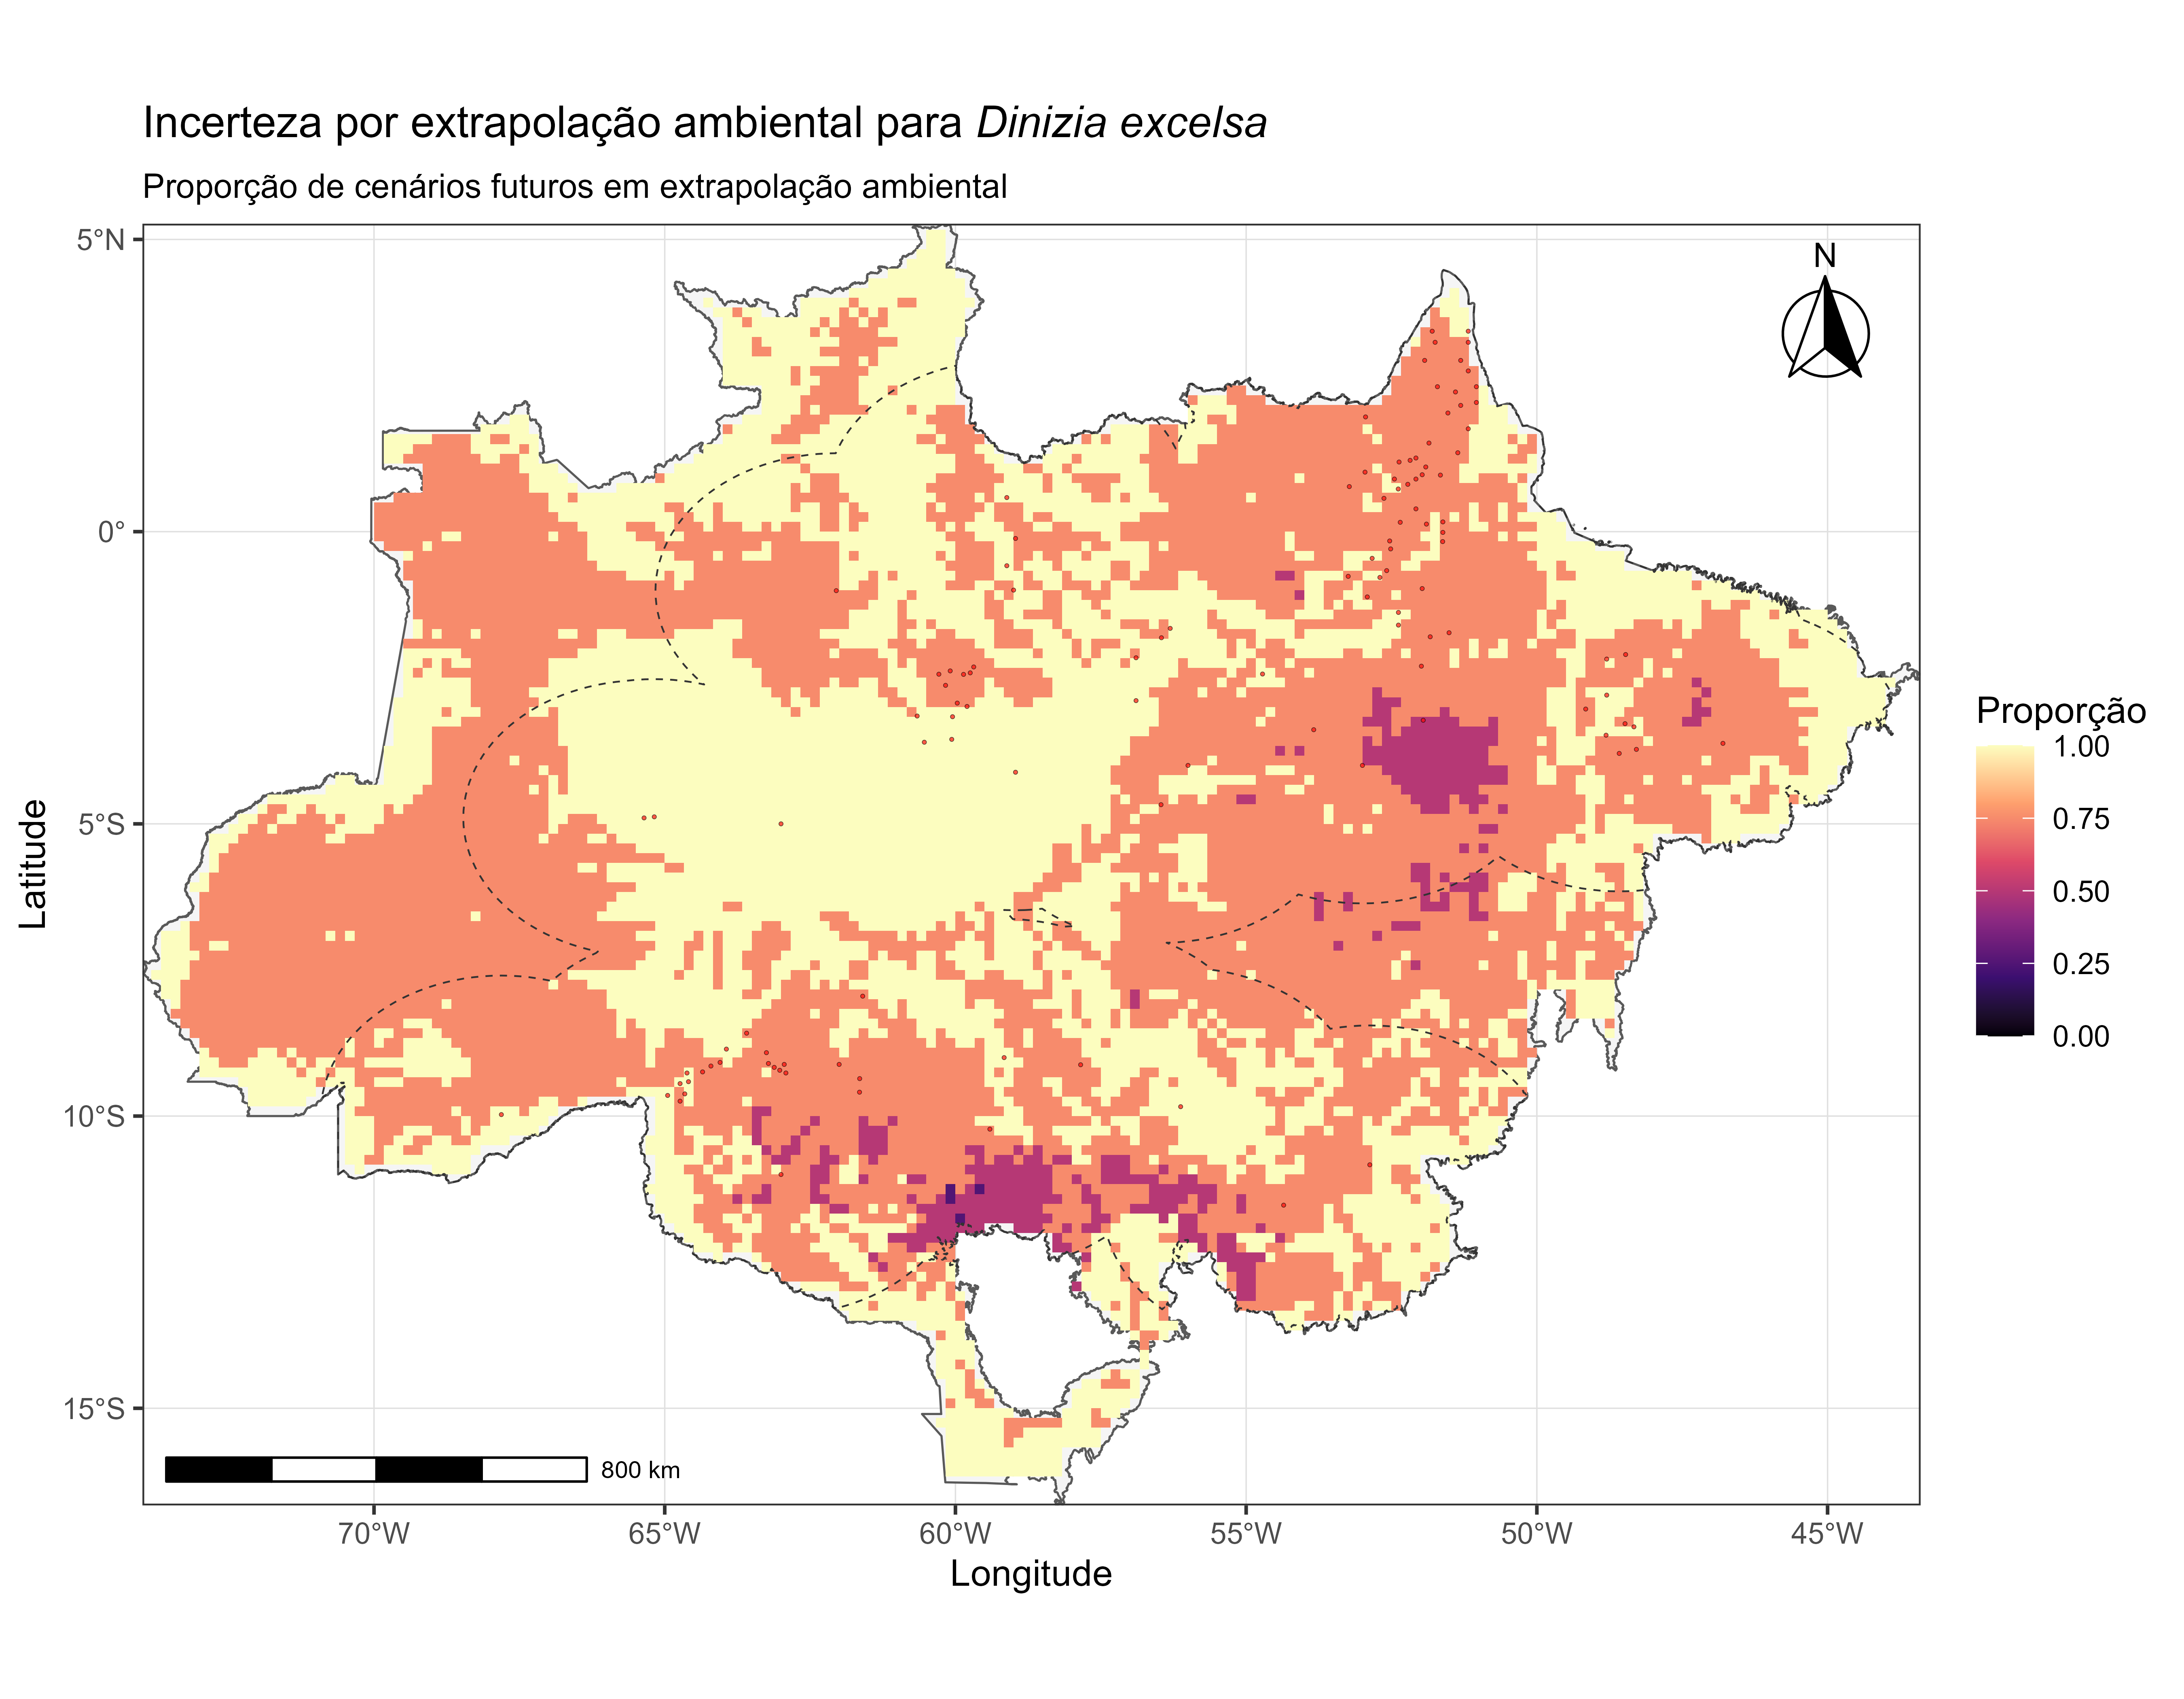
\includegraphics[width=0.96\textwidth]{figuras/unidade16/unidade16_incerteza_extrapolacao.png}
\caption{Environmental extrapolation risk in future projections for \textit{Dinizia excelsa}.}
\label{fig:unidade16_incerteza_extrapolacao}
\end{figure}

Novelty should therefore be reported alongside, rather than silently converted into, a prediction variance. A cell with low disagreement among algorithms can still be unsupported if all algorithms extrapolate similarly beyond the calibration data.

\section{Uncertainty in paleoclimate projections}

Paleoclimate applications include uncertainty from GCM structure, boundary conditions, downscaling, spatial resolution, reconstruction of past climates, predictor harmonization, and the assumption of niche conservatism. Uncertainty is best assessed by comparing alternative reconstructions for the same period and by propagating algorithmic and calibration variation within each reconstruction.

\rscriptfile{scripts/unidade16/05_incerteza_paleoclimatica.R}

\begin{figure}[H]
\centering
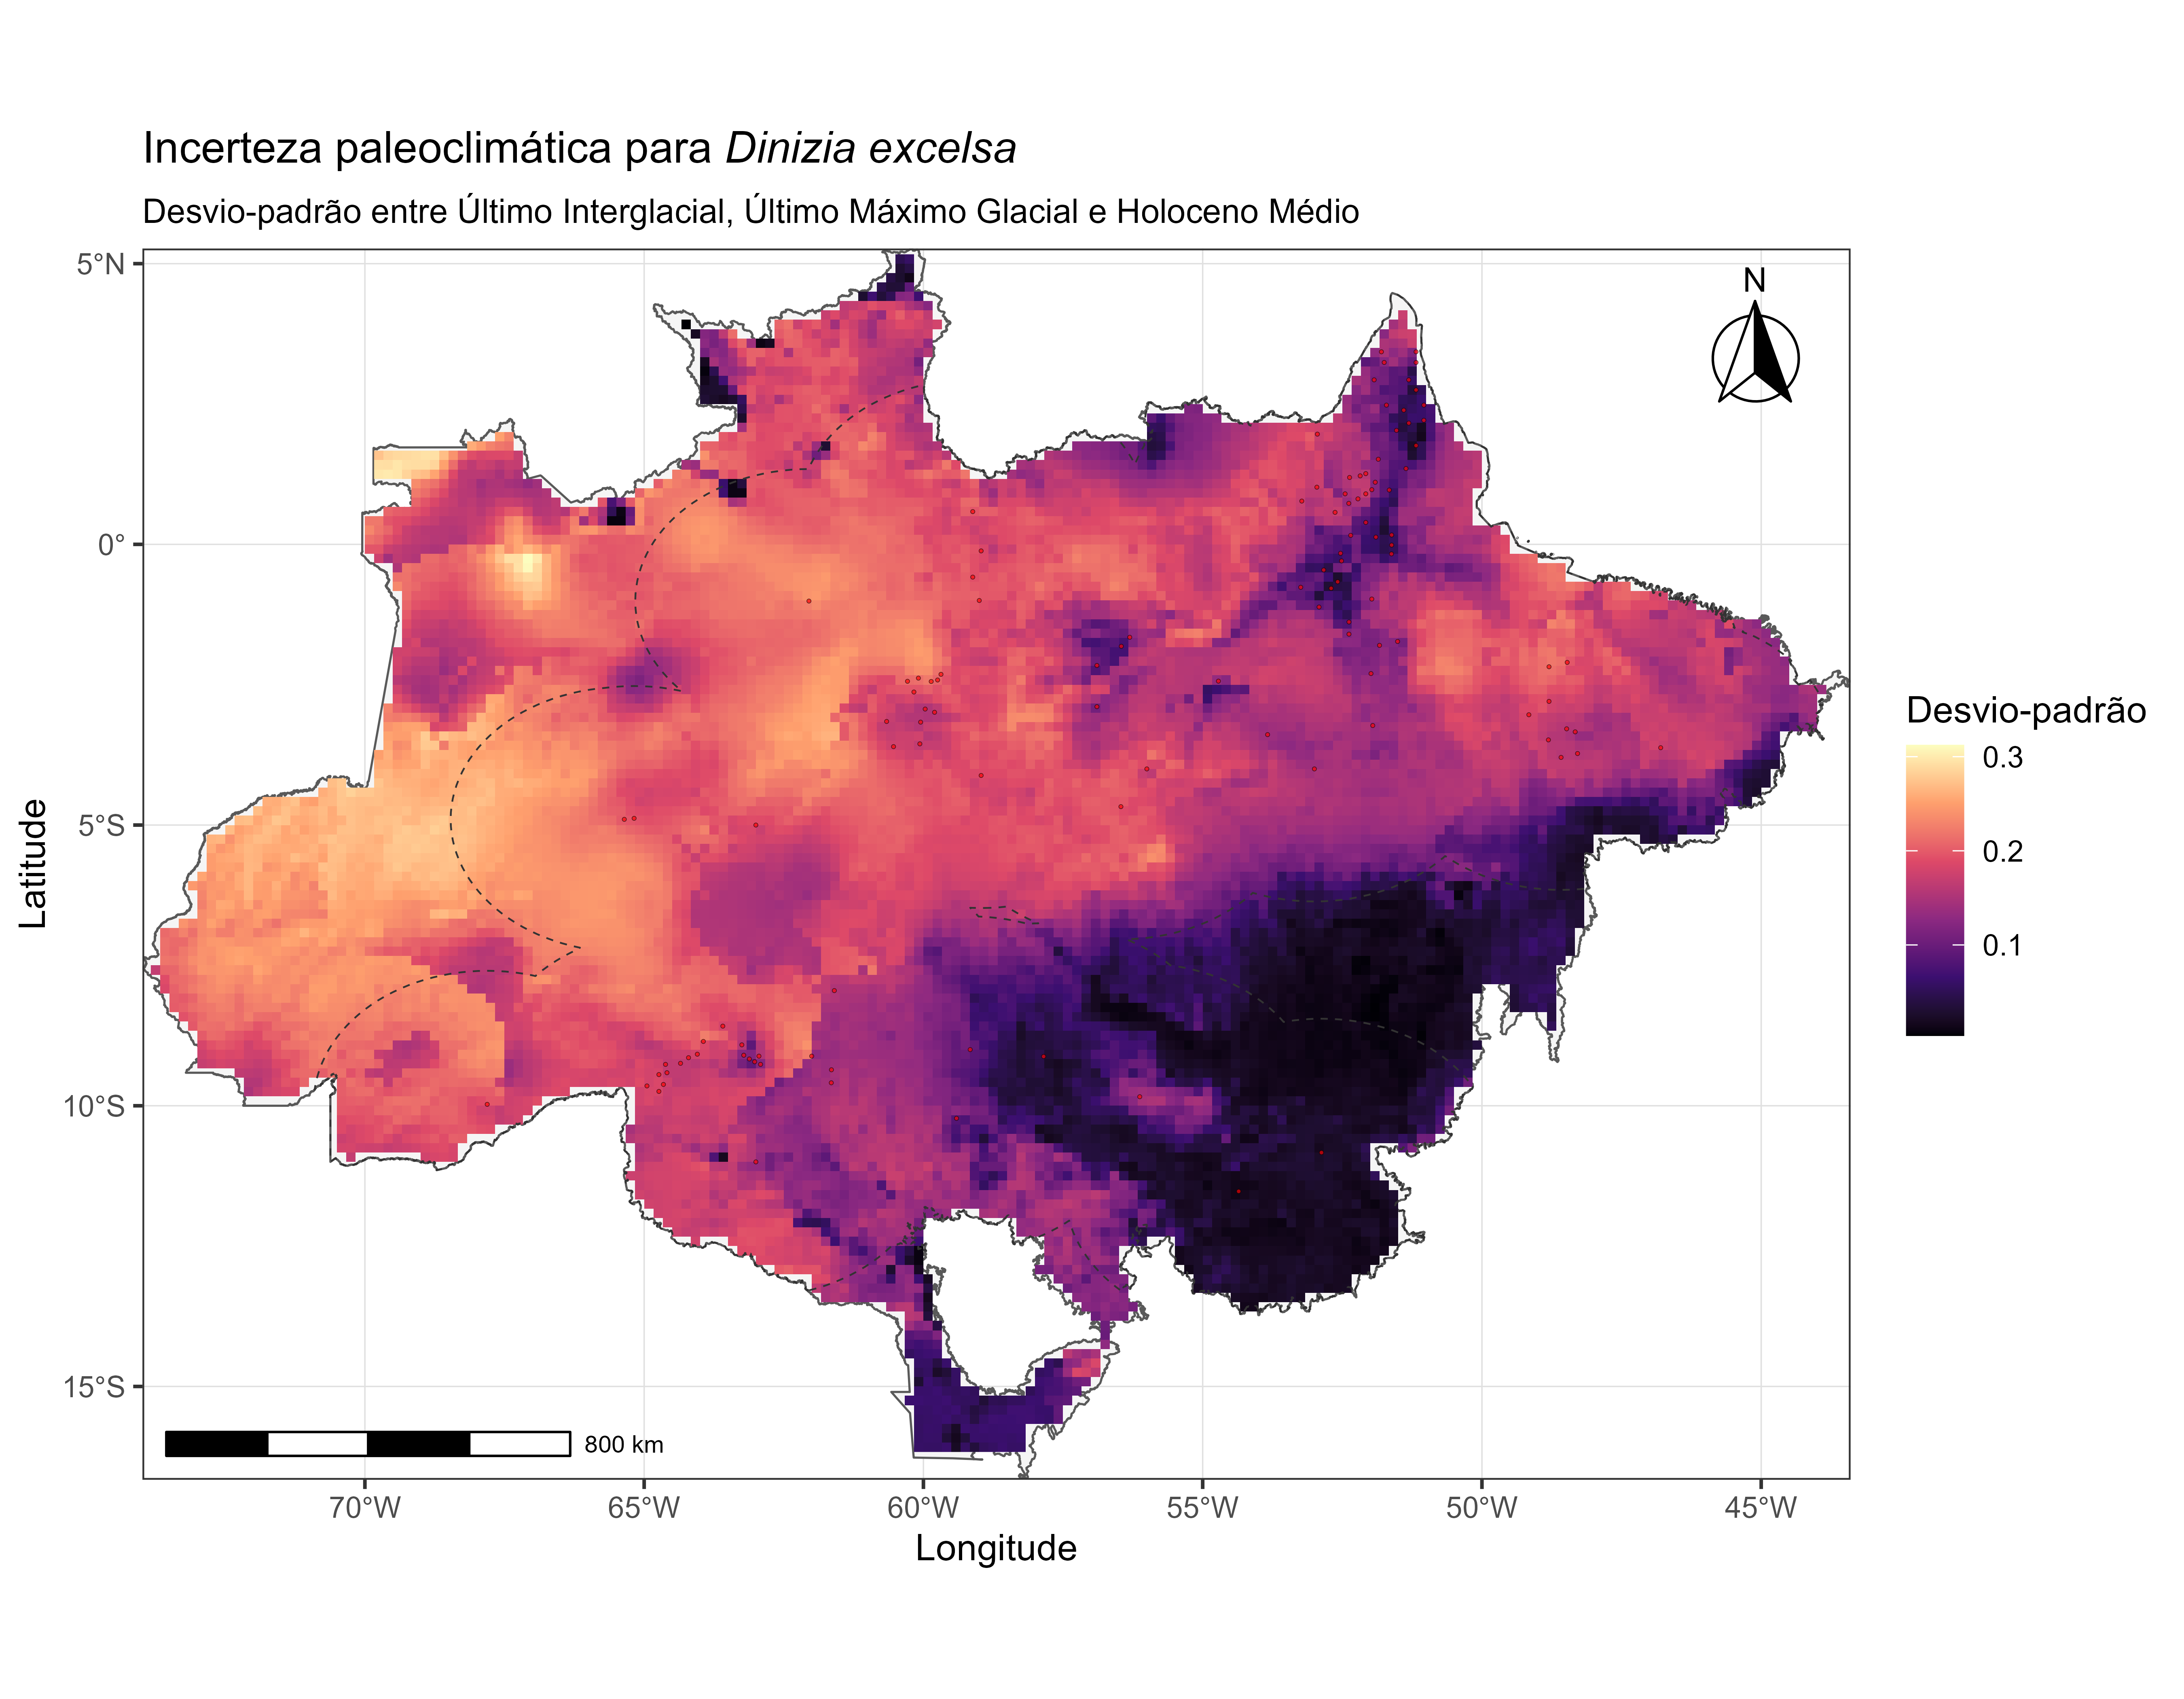
\includegraphics[width=0.88\textwidth]{figuras/unidade16/unidade16_incerteza_paleoclimatica.png}
\caption{Variation among paleoclimate projections for \textit{Dinizia excelsa}.}
\label{fig:unidade16_incerteza_paleo}
\end{figure}

Variation among the Last Interglacial, Last Glacial Maximum, and mid-Holocene is principally a temporal signal, not a replicate-based estimate of paleoclimate uncertainty. The workflow's cross-period map is useful as a stability diagnostic, but it should be labeled accordingly. A defensible uncertainty estimate would compare plausible GCMs or reconstructions within the same time slice.

\section{Integrated uncertainty indicators}

An integrated surface can summarize several diagnostics and highlight cells in which interpretation deserves caution.

\rscriptfile{scripts/unidade16/06_incerteza_integrada.R}

\begin{figure}[H]
\centering
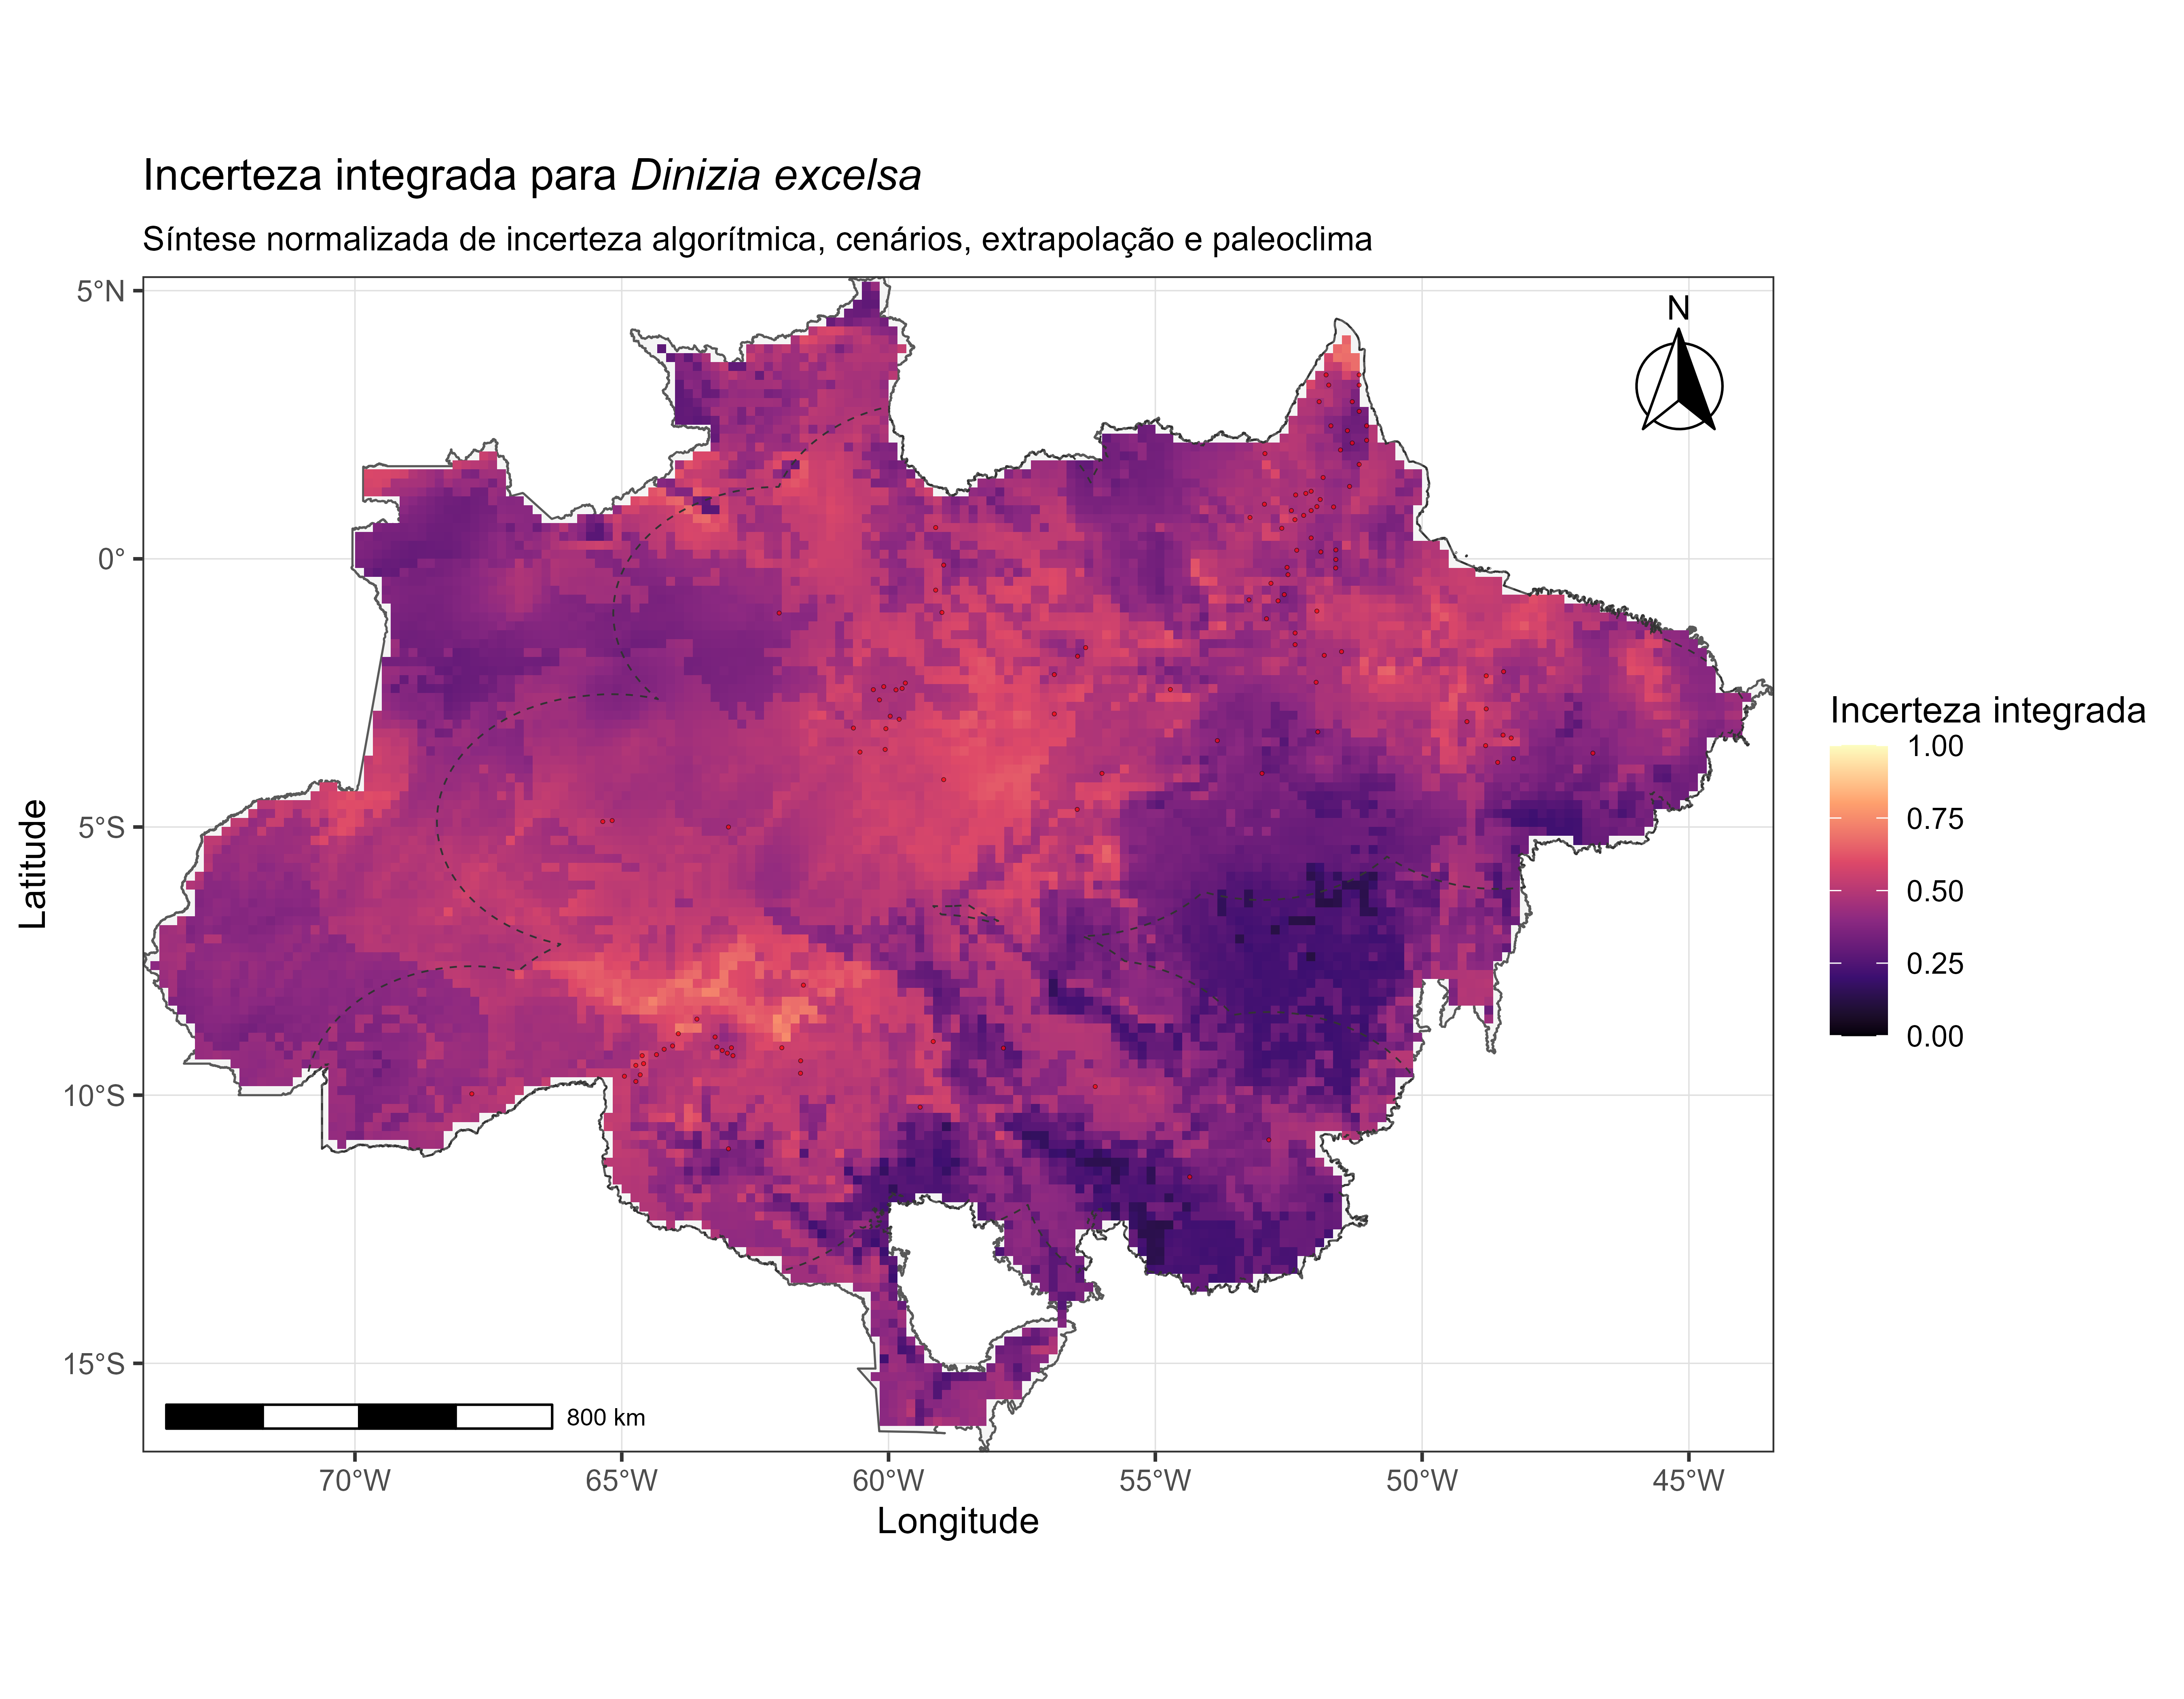
\includegraphics[width=0.88\textwidth]{figuras/unidade16/unidade16_incerteza_integrada.png}
\caption{Integrated caution index for \textit{Dinizia excelsa}, combining algorithmic disagreement, variation among future scenarios, environmental novelty, and paleoclimate variation.}
\label{fig:unidade16_incerteza_integrada}
\end{figure}

The combined surface should be called an \emph{index}, rather than a total variance, unless the components arise from a formally specified probabilistic model. Before aggregation, each component requires an explicit direction, scale, transformation, and weight. Normalizing all components to 0--1 makes them numerically combinable but does not make them conceptually equivalent. The unaggregated component maps must remain available so readers can see why a cell received a high index value.

\begin{atencao}[title={\faExclamationTriangle\quad Avoid double counting}]
Components may be dependent. Algorithmic spread can increase in novel environments, and scenario spread can include climate-model differences already summarized elsewhere. Adding correlated diagnostics can count the same source more than once. Document the dependency structure and test the sensitivity of the index to alternative weights.
\end{atencao}

\section{Suitability and uncertainty together}

Conservation interpretation benefits from considering predicted suitability and evidential support simultaneously. High-suitability, low-disagreement, environmentally analogous areas may represent relatively robust candidates. High-suitability areas with strong novelty or model disagreement are priority targets for verification, not automatically low-priority areas.

\rscriptfile{scripts/unidade16/07_adequabilidade_incerteza.R}

\begin{figure}[H]
\centering
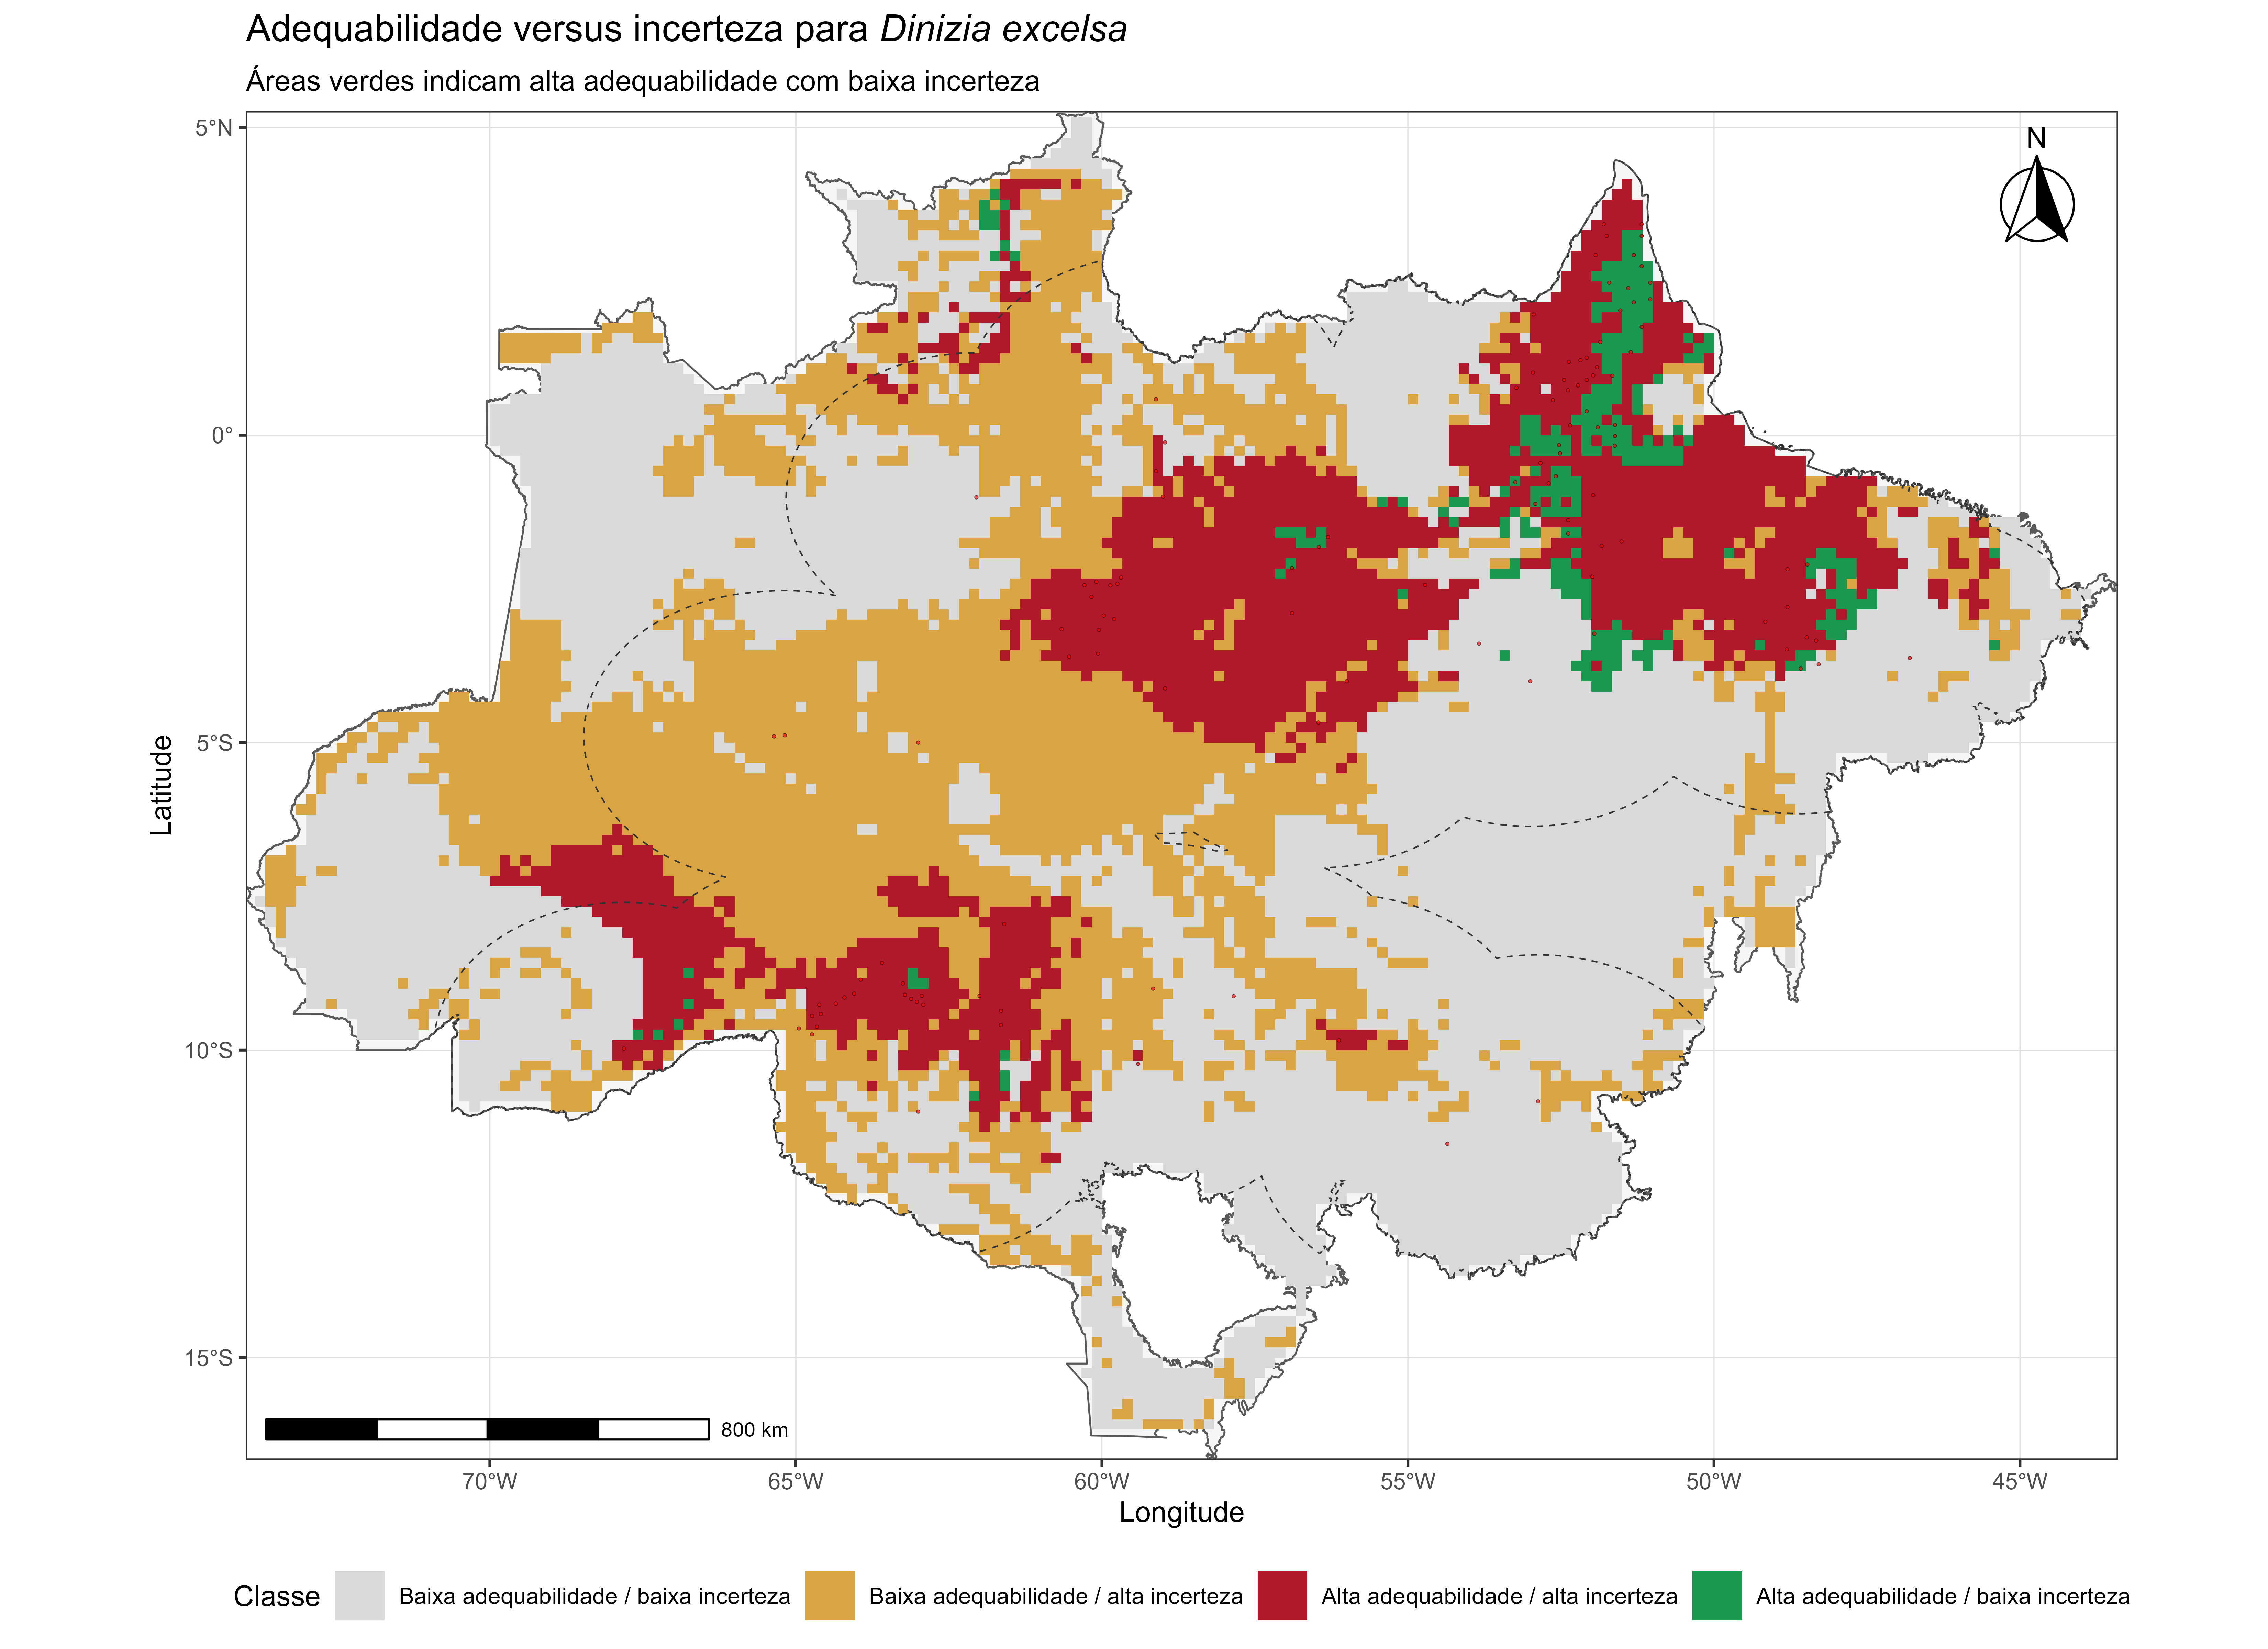
\includegraphics[width=0.96\textwidth]{figuras/unidade16/unidade16_adequabilidade_incerteza.png}
\caption{Joint classification of modeled suitability and the integrated uncertainty indicator for \textit{Dinizia excelsa}.}
\label{fig:unidade16_adequabilidade_incerteza}
\end{figure}

Classification cutoffs must be declared and subjected to sensitivity analysis. A high-versus-low matrix is a communication device and should not replace continuous surfaces, component diagnostics, or decision-specific costs.

\section{Quantitative synthesis}

\rscriptfile{scripts/unidade16/08_sintese_incertezas.R}

\begin{figure}[H]
\centering
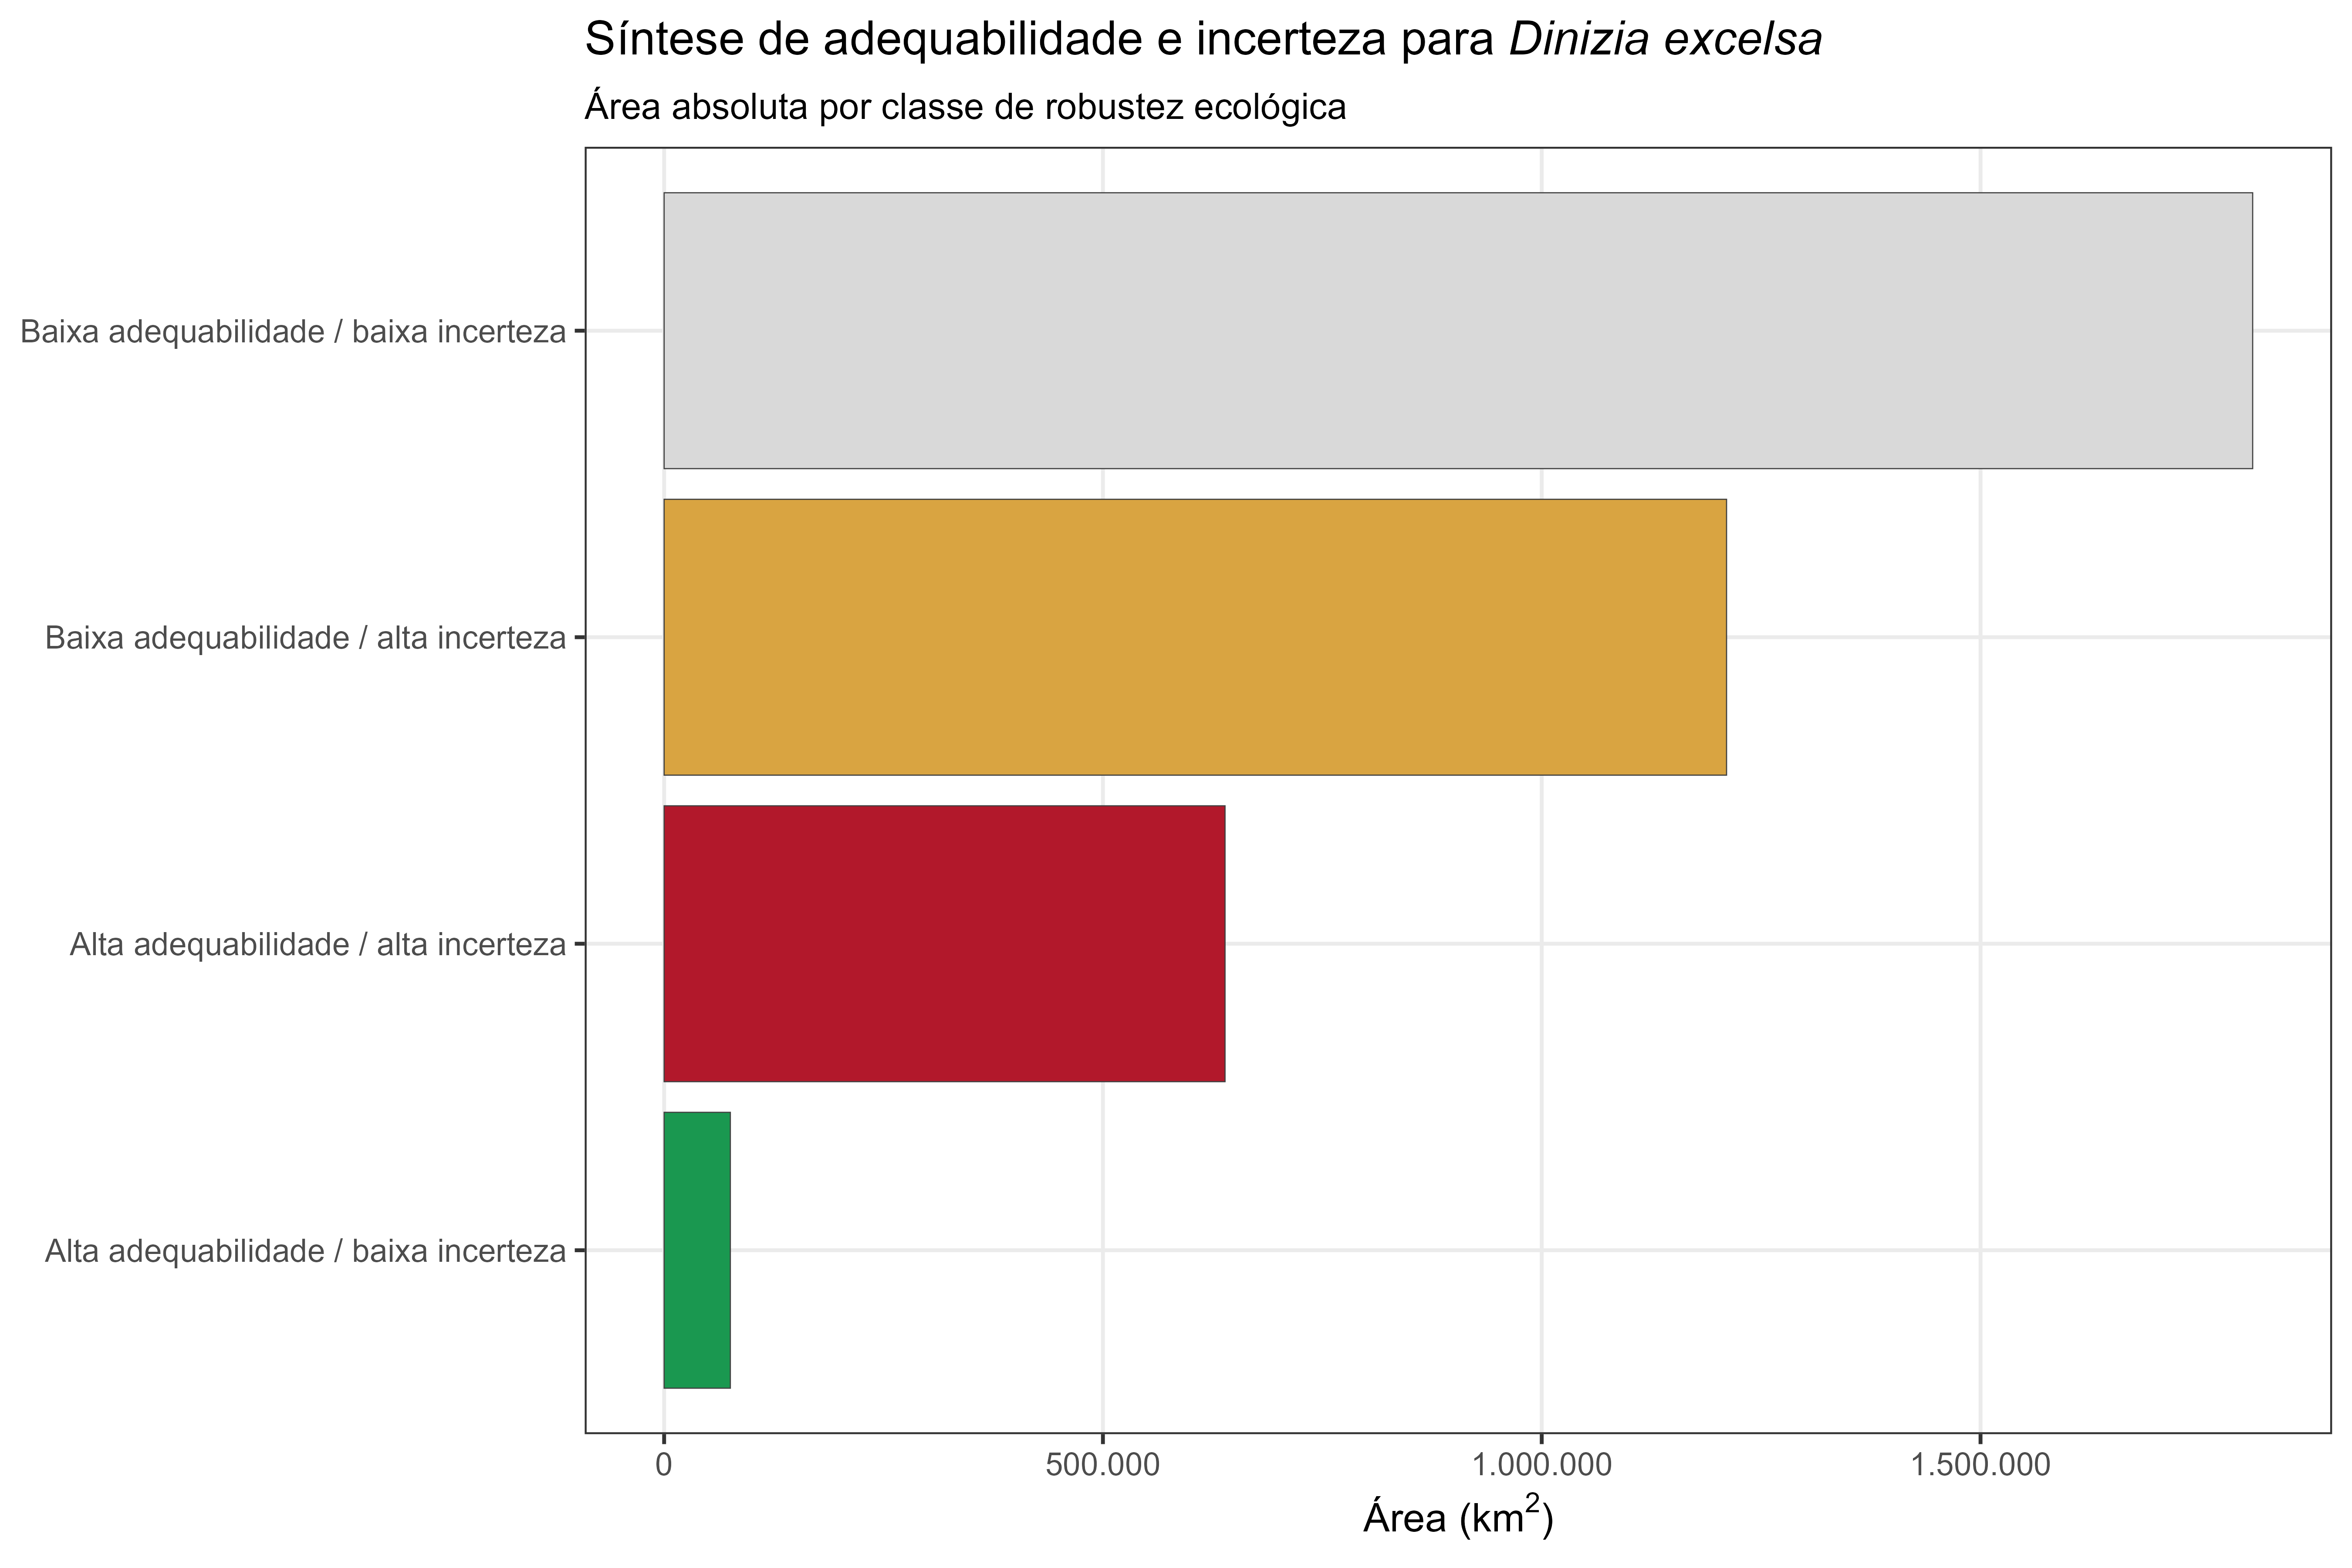
\includegraphics[width=0.88\textwidth]{figuras/unidade16/unidade16_sintese_incertezas.png}
\caption{Quantitative summary of joint suitability and uncertainty-index classes for \textit{Dinizia excelsa}.}
\label{fig:unidade16_sintese}
\end{figure}

Useful reporting includes maps and distributions for each component, factorial summaries by model and scenario, agreement on the sign of change, threshold sensitivity, and the proportion of the decision area supported by analogous environments. Where computationally feasible, resampling occurrences and calibration folds helps propagate sampling and estimation uncertainty.

\section{Complete pipeline}

\rscriptfile{scripts/unidade16/09_pipeline_incertezas.R}

\section{Chapter synthesis}

Uncertainty analysis turns SDM from a single cartographic product into a more transparent inferential workflow. For \textit{Dinizia excelsa}, separating algorithmic disagreement, conditional scenario variation, climate-model effects, paleoclimate reconstruction, and environmental novelty clarifies which conclusions are stable and which remain hypotheses.

\begin{conceito}[title={\faBook\quad Key message}]
Every SDM interpretation should ask two linked questions: what does the model estimate, and how strongly do the available data and assumptions support that estimate? No single standard-deviation map answers the second question completely.
\end{conceito}

\section{Review exercises}

\begin{enumerate}
\item Distinguish uncertainty, variability, disagreement, novelty, and bias using SDM examples.
\item What does the cellwise standard deviation among algorithms measure, and why is it not a confidence interval?
\item Why is variation among SSPs not automatically a probabilistic estimate of uncertainty?
\item How do MESS and MOP inform evidential support without directly measuring prediction error?
\item Why is variation among different paleoclimatic periods a temporal signal rather than a pure uncertainty estimate?
\item How should high suitability combined with high novelty or disagreement be interpreted?
\item What information must accompany an integrated uncertainty index used in conservation planning?
\end{enumerate}


\chapter[Conservation applications]{Applications of Species Distribution Models in Conservation}

\begin{objetivos}
By the end of this chapter, readers should be able to explain how SDMs can inform conservation decisions; combine contemporary suitability, future climatic stability, uncertainty indicators, and protected-area coverage; identify candidate priority areas for \textit{Dinizia excelsa}; assess representation and protection gaps; construct transparent spatial-priority indices; and discuss applications to threatened species, giant trees, ecological restoration, monitoring, and systematic conservation planning.
\end{objetivos}

\section{Introduction}

Species distribution models are widely used to support conservation under climate change, habitat loss, forest fragmentation, and expanding human pressure. Their role is not merely to map where a species could find suitable environmental conditions. Conservation decisions also require information about persistence, threats, connectivity, representation, feasibility, costs, governance, and uncertainty \parencite{margules2000systematic,moilanen2009spatial,franklin2023,guisan2017habitat,zurell2020benchmarking}.

This chapter integrates products developed previously into an applied analysis for \textit{Dinizia excelsa}. The resulting maps synthesize ecological and climatic evidence for screening candidate areas. They are decision-support products, not automatic prescriptions for reserve designation or intervention.

\begin{conceito}[title={\faBook\quad SDM as conservation evidence}]
In conservation, an SDM is one spatial layer of evidence. It should be combined with protected-area status, habitat condition, connectivity, exposure to threats, uncertainty, ecological feasibility, management objectives, costs, and the rights and knowledge of affected communities.
\end{conceito}

\section{Defining the decision problem}

Before combining maps, specify the conservation objective, spatial units, planning horizon, target, and decision constraints. Protecting extant populations, restoring habitat, maintaining climatic refuges, establishing corridors, guiding surveys, and supporting assisted migration are different problems and may produce different rankings.

The didactic index in this chapter uses five criteria:

\begin{itemize}
\item high contemporary modeled suitability;
\item persistence of suitability across specified future projections;
\item modeled paleoclimatic stability;
\item a low integrated caution index;
\item representation inside or outside existing protected areas.
\end{itemize}

Protected-area overlap can serve two opposing objectives. Areas inside the network may be priorities for reinforcing management of already represented habitat, whereas suitable areas outside it may reveal representation gaps. The role of this criterion must therefore be defined before scoring.

\begin{atencao}[title={\faExclamationTriangle\quad Suitability alone does not define priority}]
A highly suitable cell may be degraded, disconnected, legally unavailable, environmentally extrapolative, or too costly to manage. Conversely, a moderately suitable cell may be essential for complementarity or connectivity. Prioritization must follow an explicit decision objective rather than a suitability ranking alone.
\end{atencao}

\section{Preparing spatial evidence}

\rscriptfile{scripts/unidade17/01_estrutura_pastas.R}

\rscriptfile{scripts/unidade17/02_preparar_camadas_conservacao.R}

All layers must share a coordinate reference system, extent, resolution, cell origin, and mask. Area calculations should use an equal-area projection or cell-area weighting. Protected-area data require a documented version and date because boundaries, legal categories, and management status can change. Overlap between polygons and raster cells should not be interpreted as effective protection without information on implementation and condition.

\section{Contemporary climatic priority}

\rscriptfile{scripts/unidade17/03_prioridade_climatica_atual.R}

\begin{figure}[H]
\centering
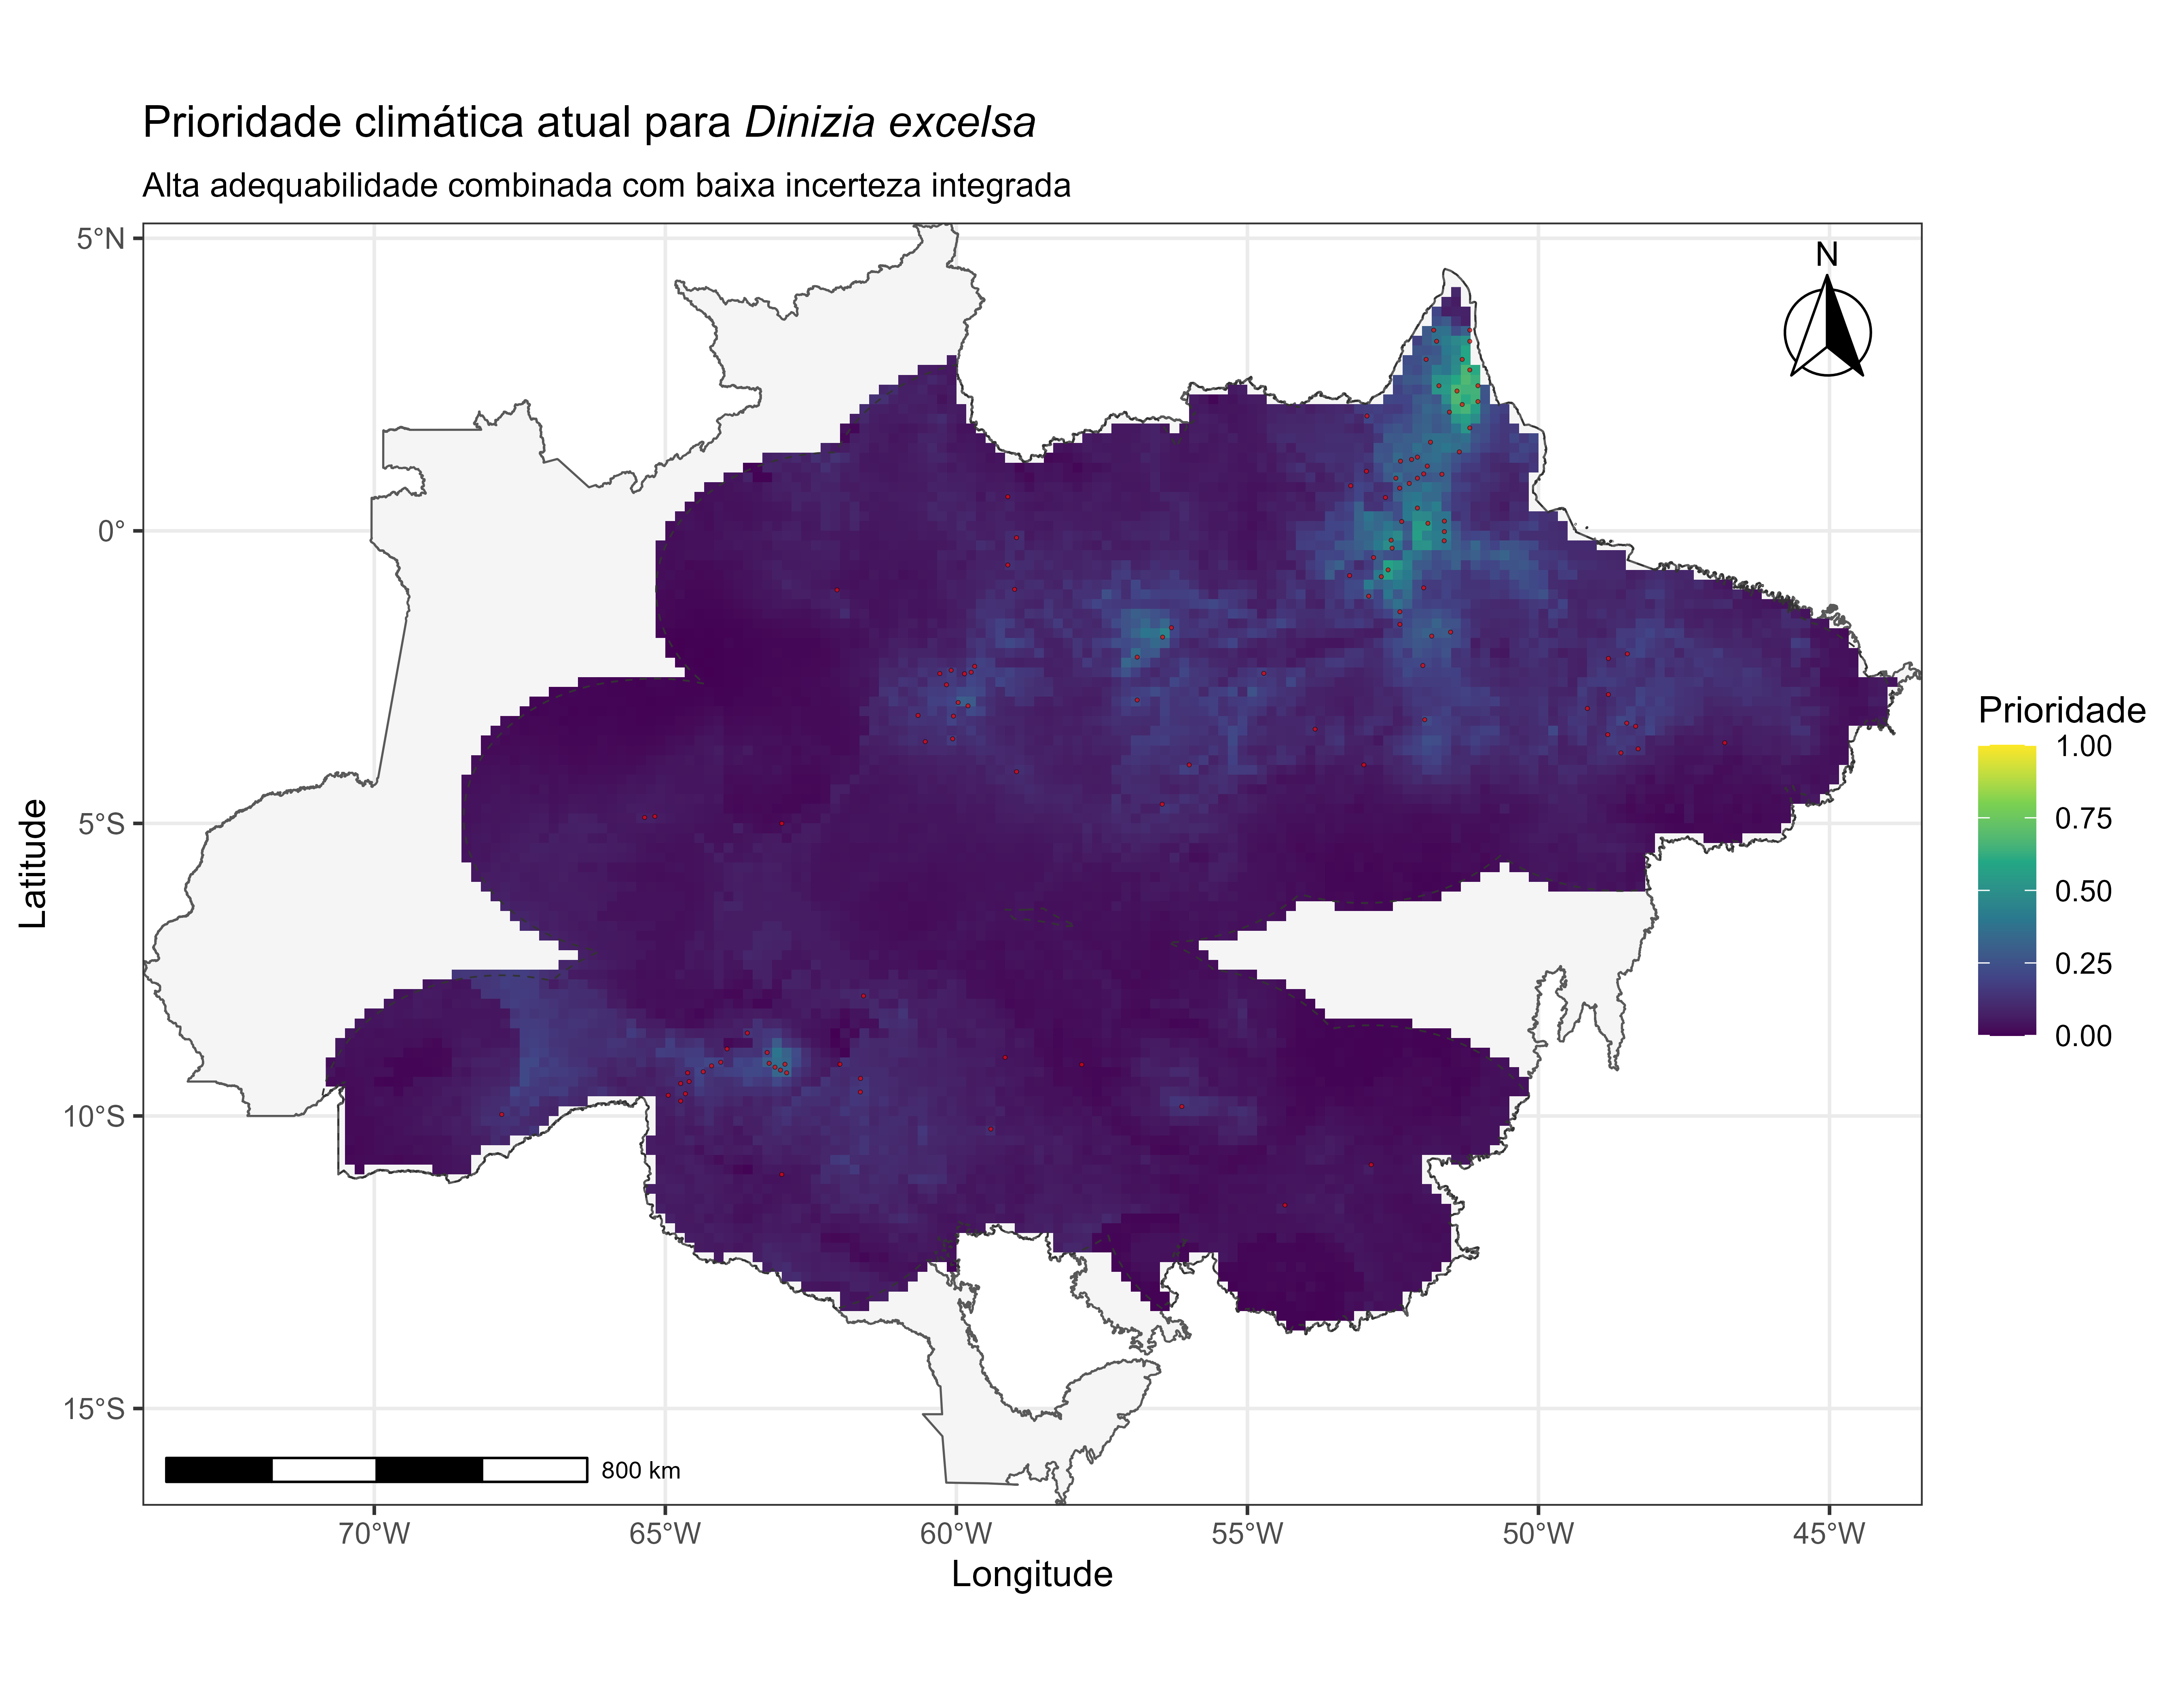
\includegraphics[width=0.88\textwidth]{figuras/unidade17/unidade17_prioridade_climatica_atual.png}
\caption{Contemporary climatic-priority index for \textit{Dinizia excelsa}, based on modeled suitability and the integrated uncertainty indicator.}
\label{fig:unidade17_prioridade_atual}
\end{figure}

This layer identifies locations where the model estimates relatively suitable contemporary conditions with comparatively strong support. It does not confirm population presence, habitat integrity, abundance, regeneration, or demographic viability. Field records and remotely sensed habitat condition should be used to validate candidate sites.

\section{Future stability and conservation}

\rscriptfile{scripts/unidade17/04_estabilidade_futura_conservacao.R}

\begin{figure}[H]
\centering
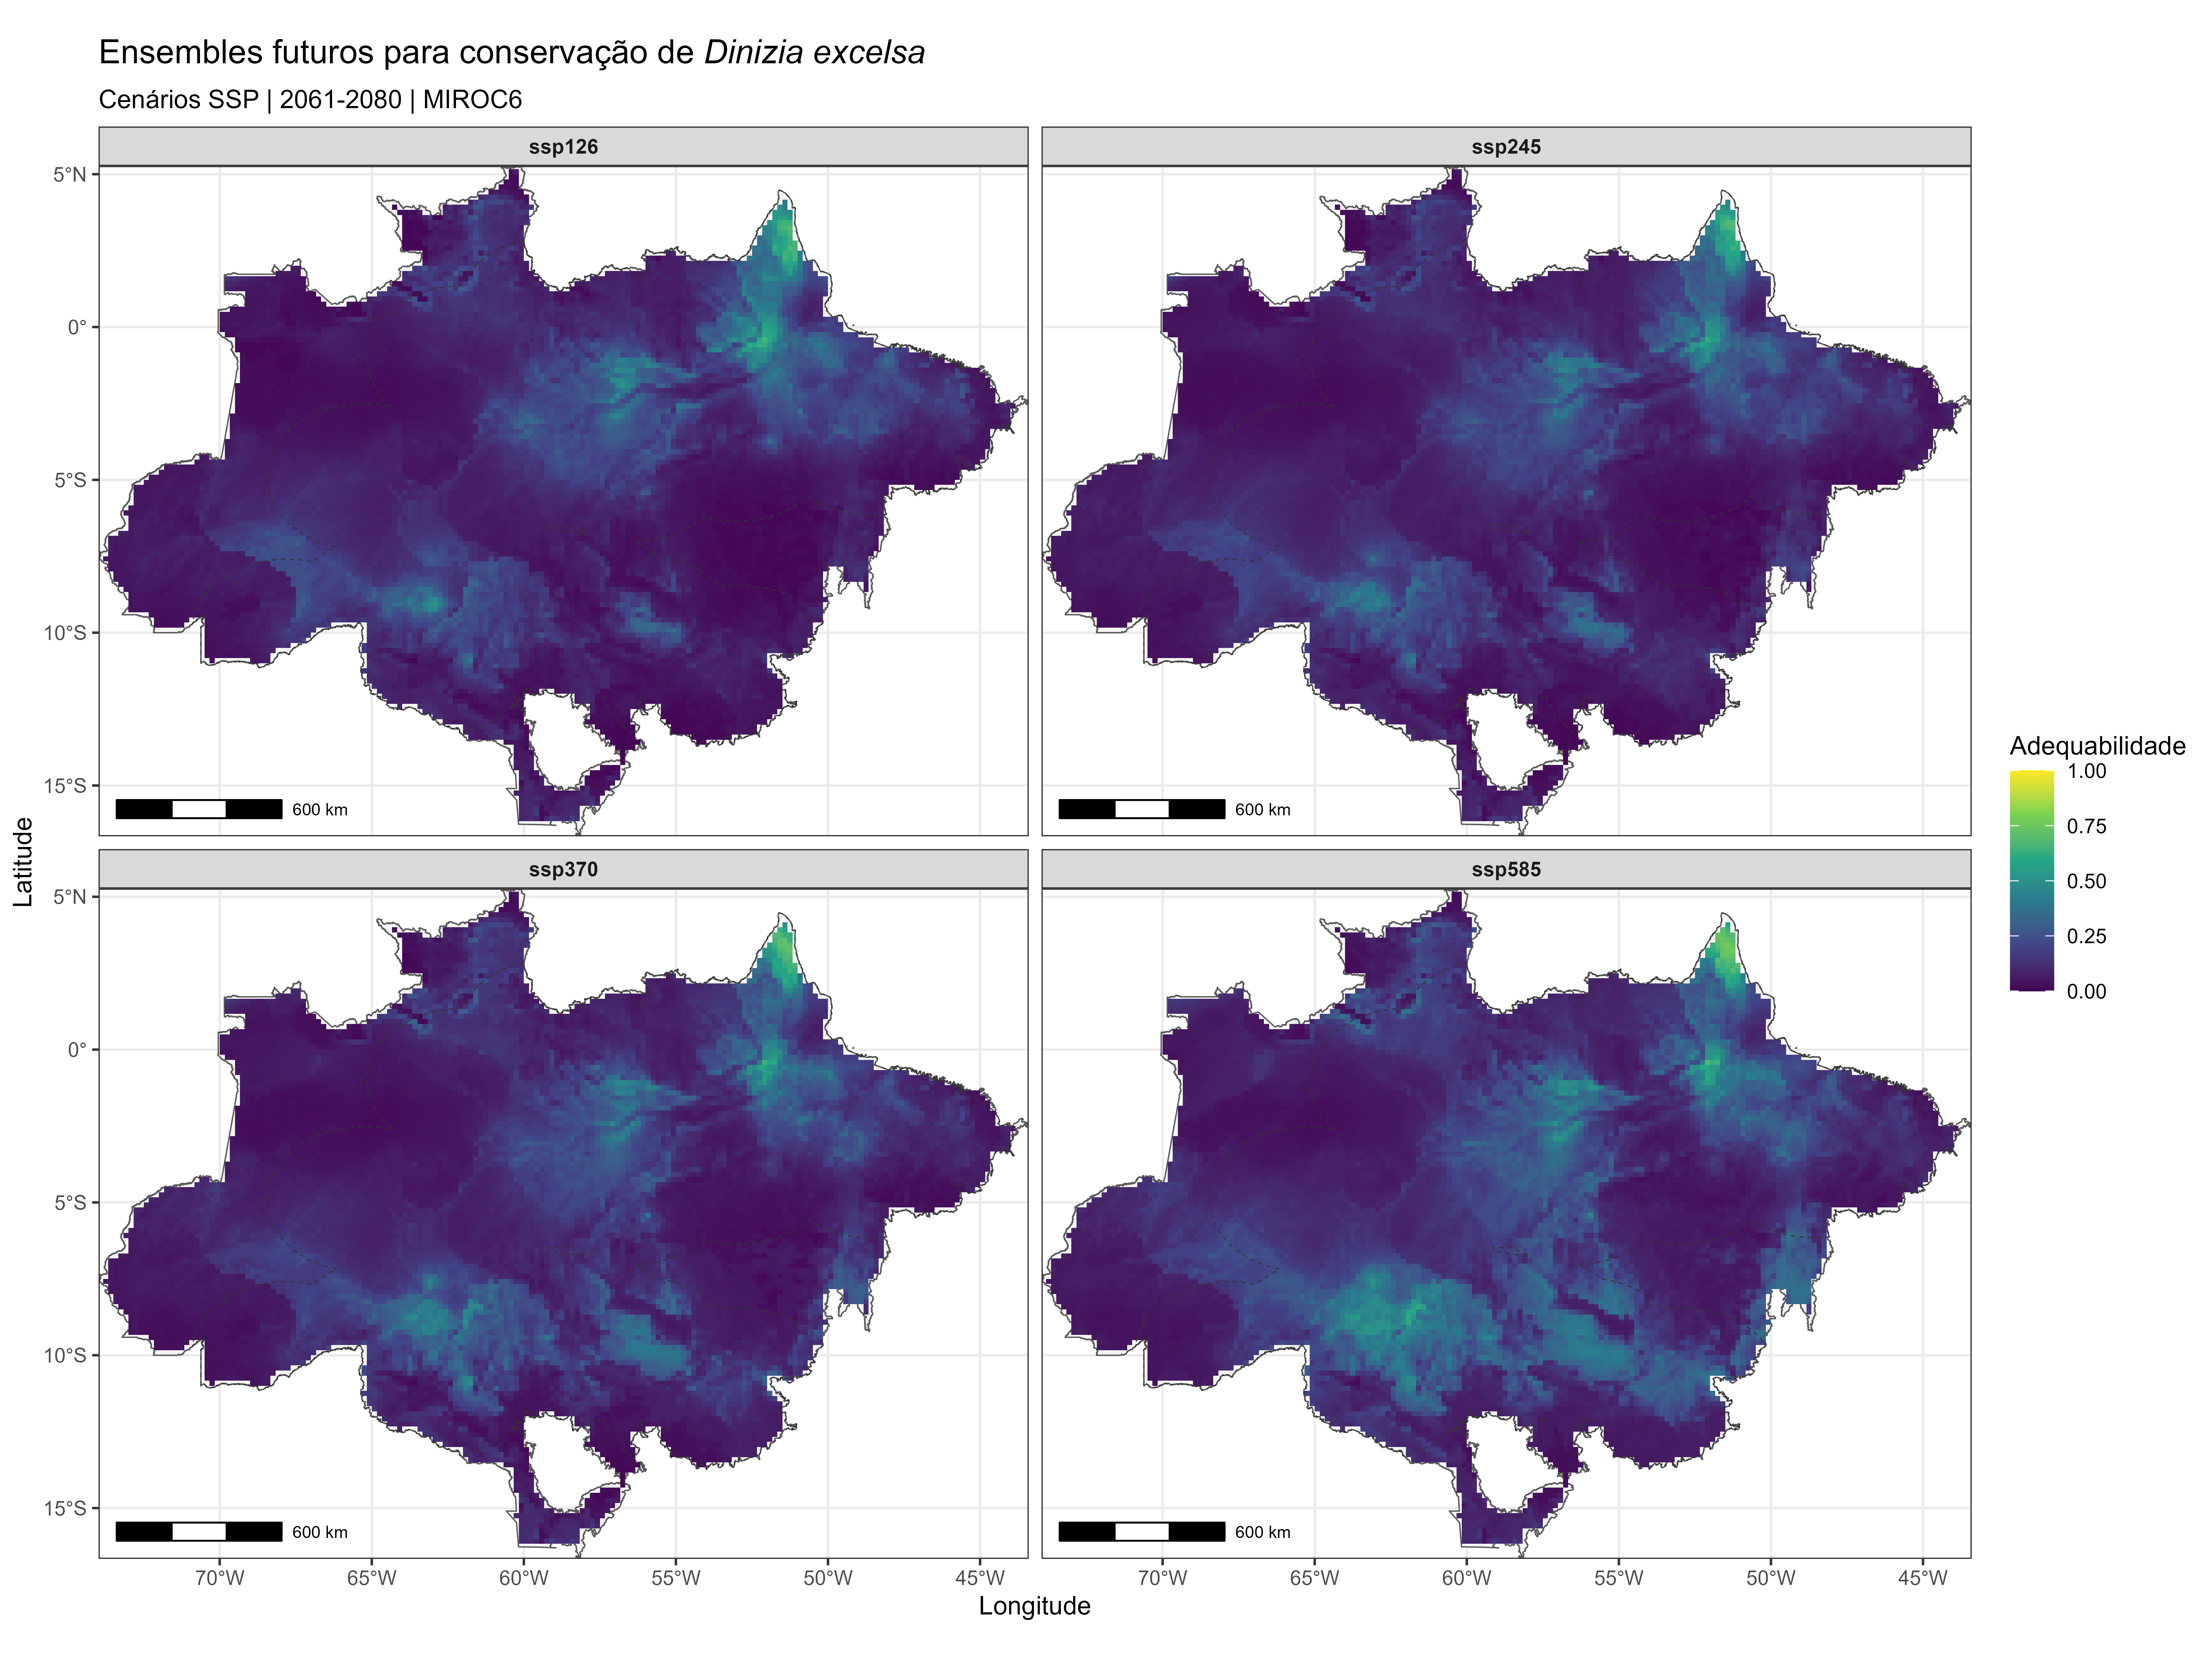
\includegraphics[width=0.96\textwidth]{figuras/unidade17/unidade17_estabilidade_futura_conservacao.png}
\caption{Persistence of projected environmental suitability for \textit{Dinizia excelsa} across specified future climate scenarios.}
\label{fig:unidade17_estabilidade_futura}
\end{figure}

Future stability is conditional on the GCMs, SSPs, time horizons, thresholds, algorithms, and assumptions selected. Requiring agreement across all scenarios is conservative but may discard areas valuable under most futures; averaging scenarios can conceal directional disagreement. Report the chosen robustness rule and test alternatives.

\section{Historical stability and candidate climatic refugia}

\rscriptfile{scripts/unidade17/05_refugios_climaticos_conservacao.R}

\begin{figure}[H]
\centering
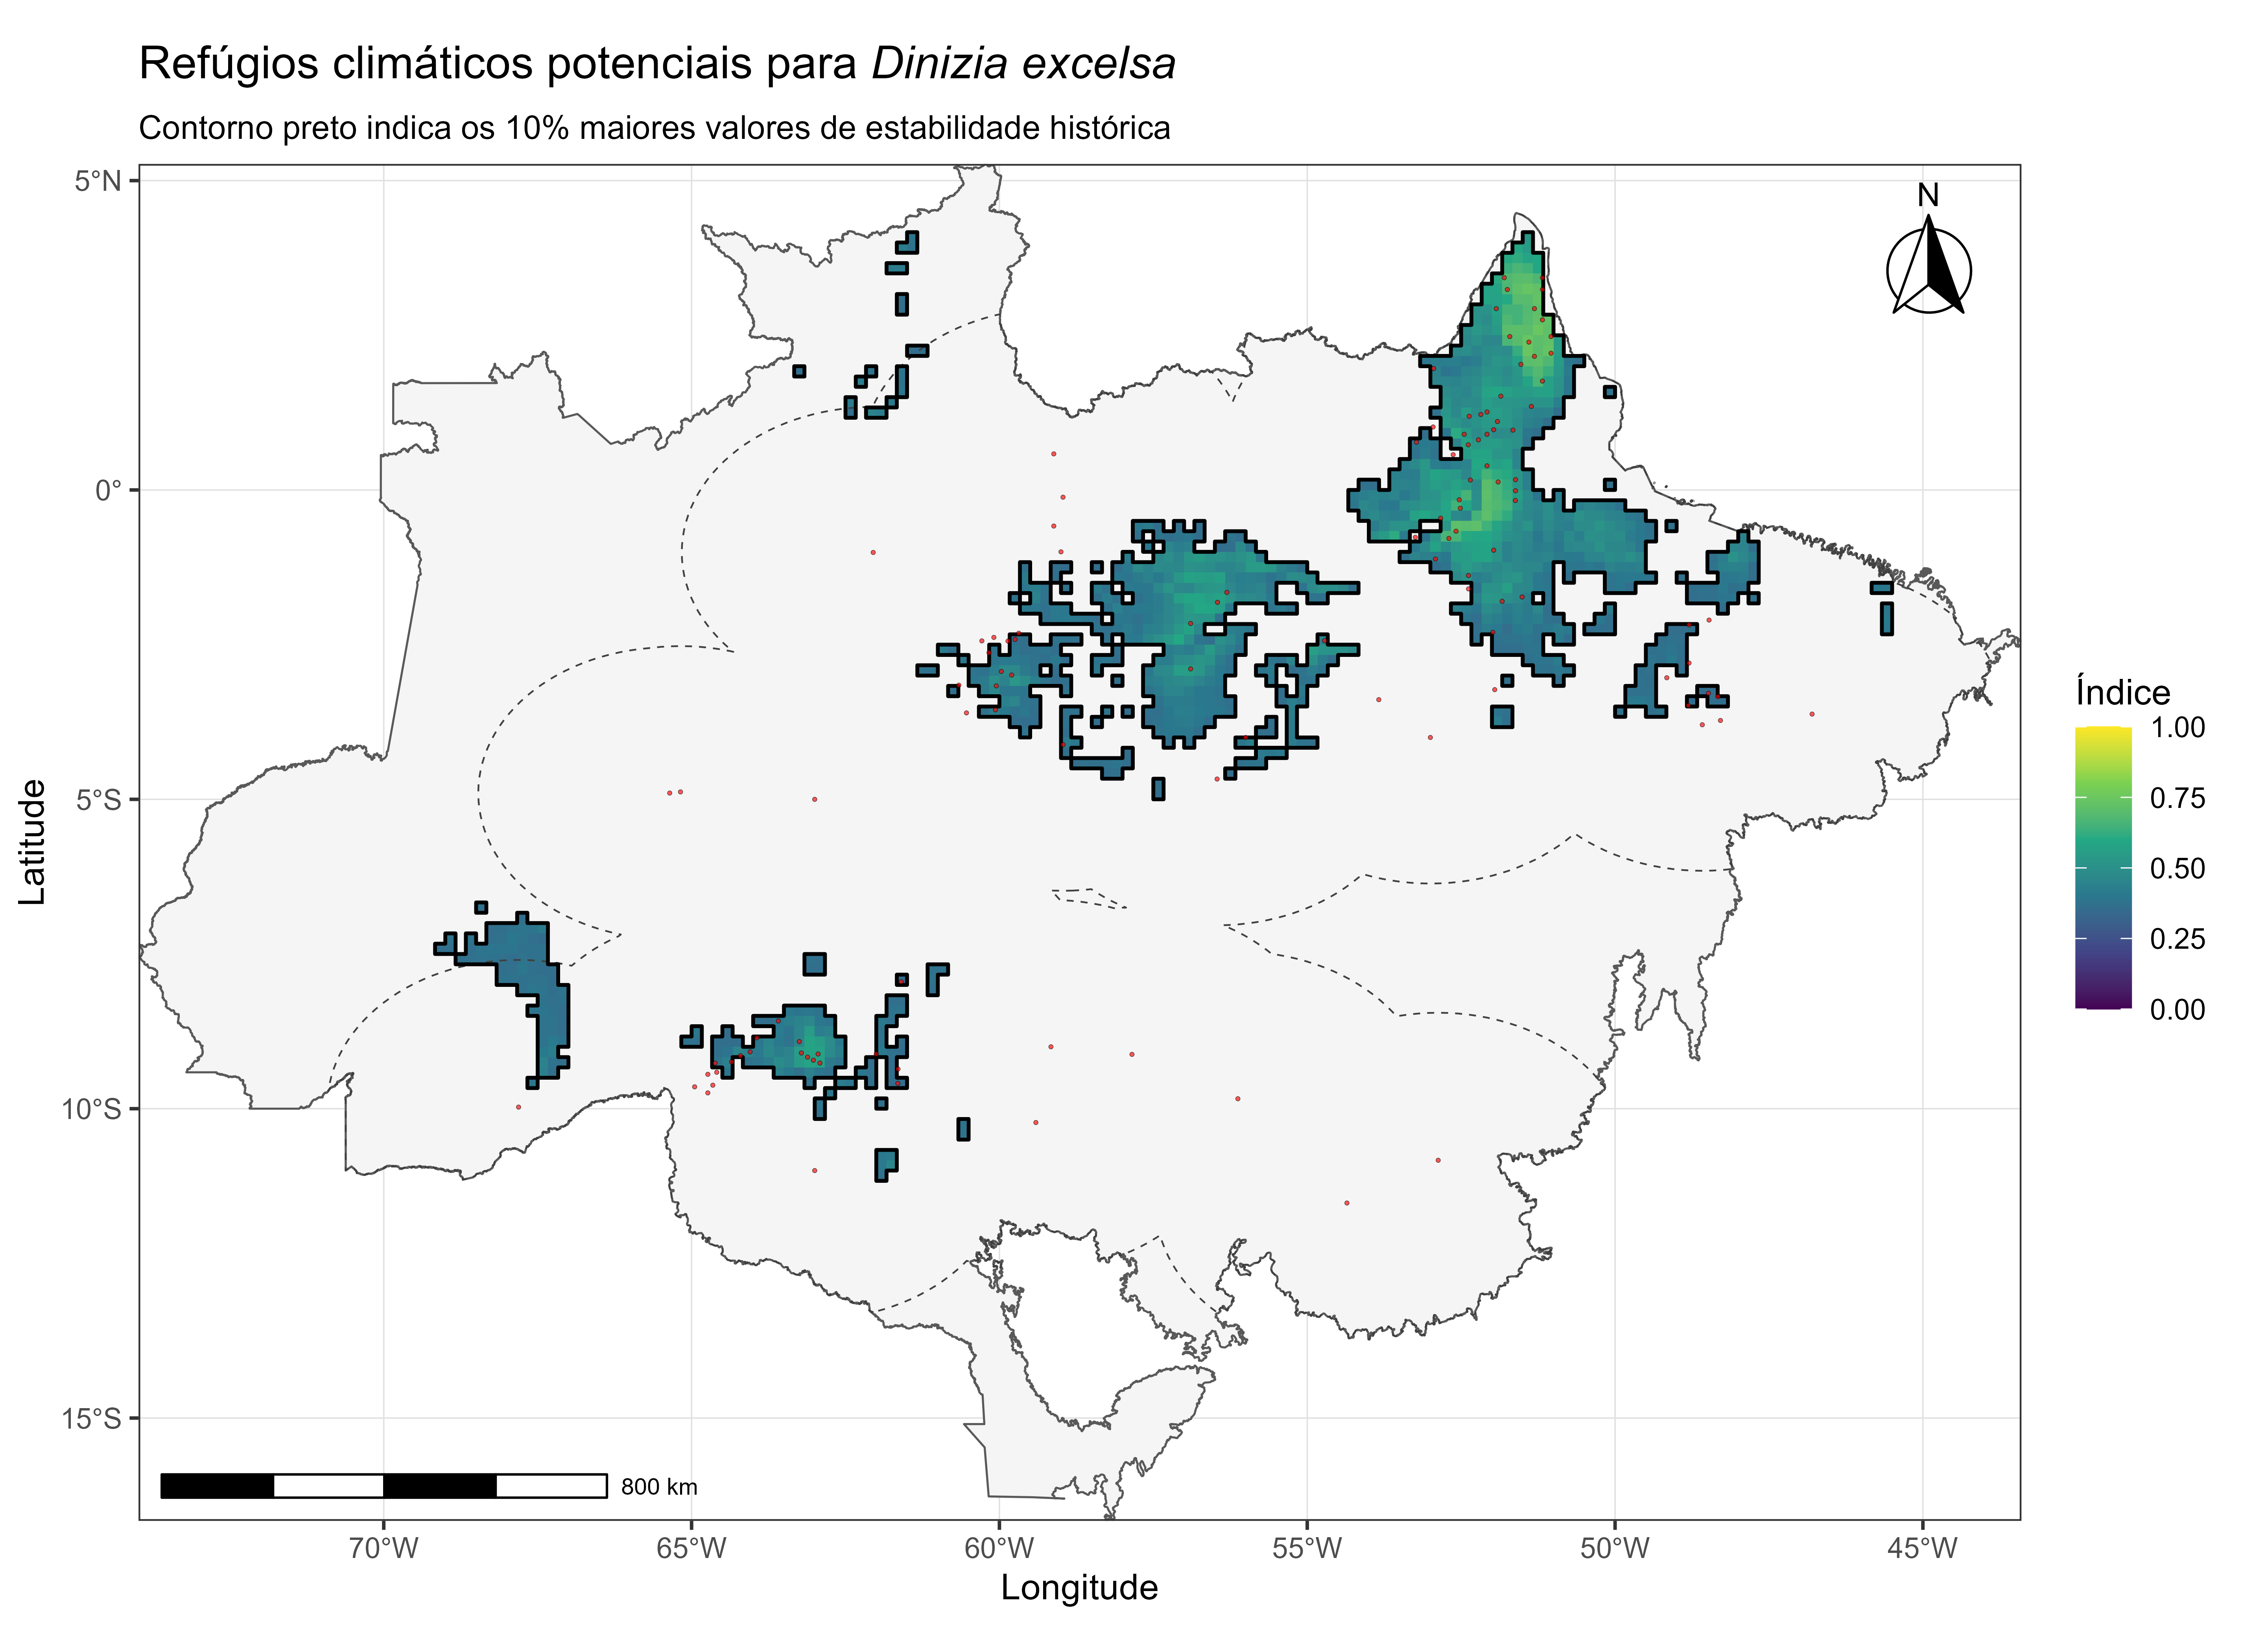
\includegraphics[width=0.96\textwidth]{figuras/unidade17/unidade17_refugios_climaticos.png}
\caption{Candidate areas of long-term climatic suitability for \textit{Dinizia excelsa}, integrating contemporary and paleoclimatic projections.}
\label{fig:unidade17_refugios}
\end{figure}

Persistent modeled suitability identifies climatic-stability candidates, not demonstrated refugia. Conservation claims should be corroborated with phylogeographic, paleoecological, demographic, floristic, or genetic evidence and evaluated against environmental novelty in past projections.

\section{Representation and protection gaps}

\rscriptfile{scripts/unidade17/06_lacunas_protecao.R}

\begin{figure}[H]
\centering
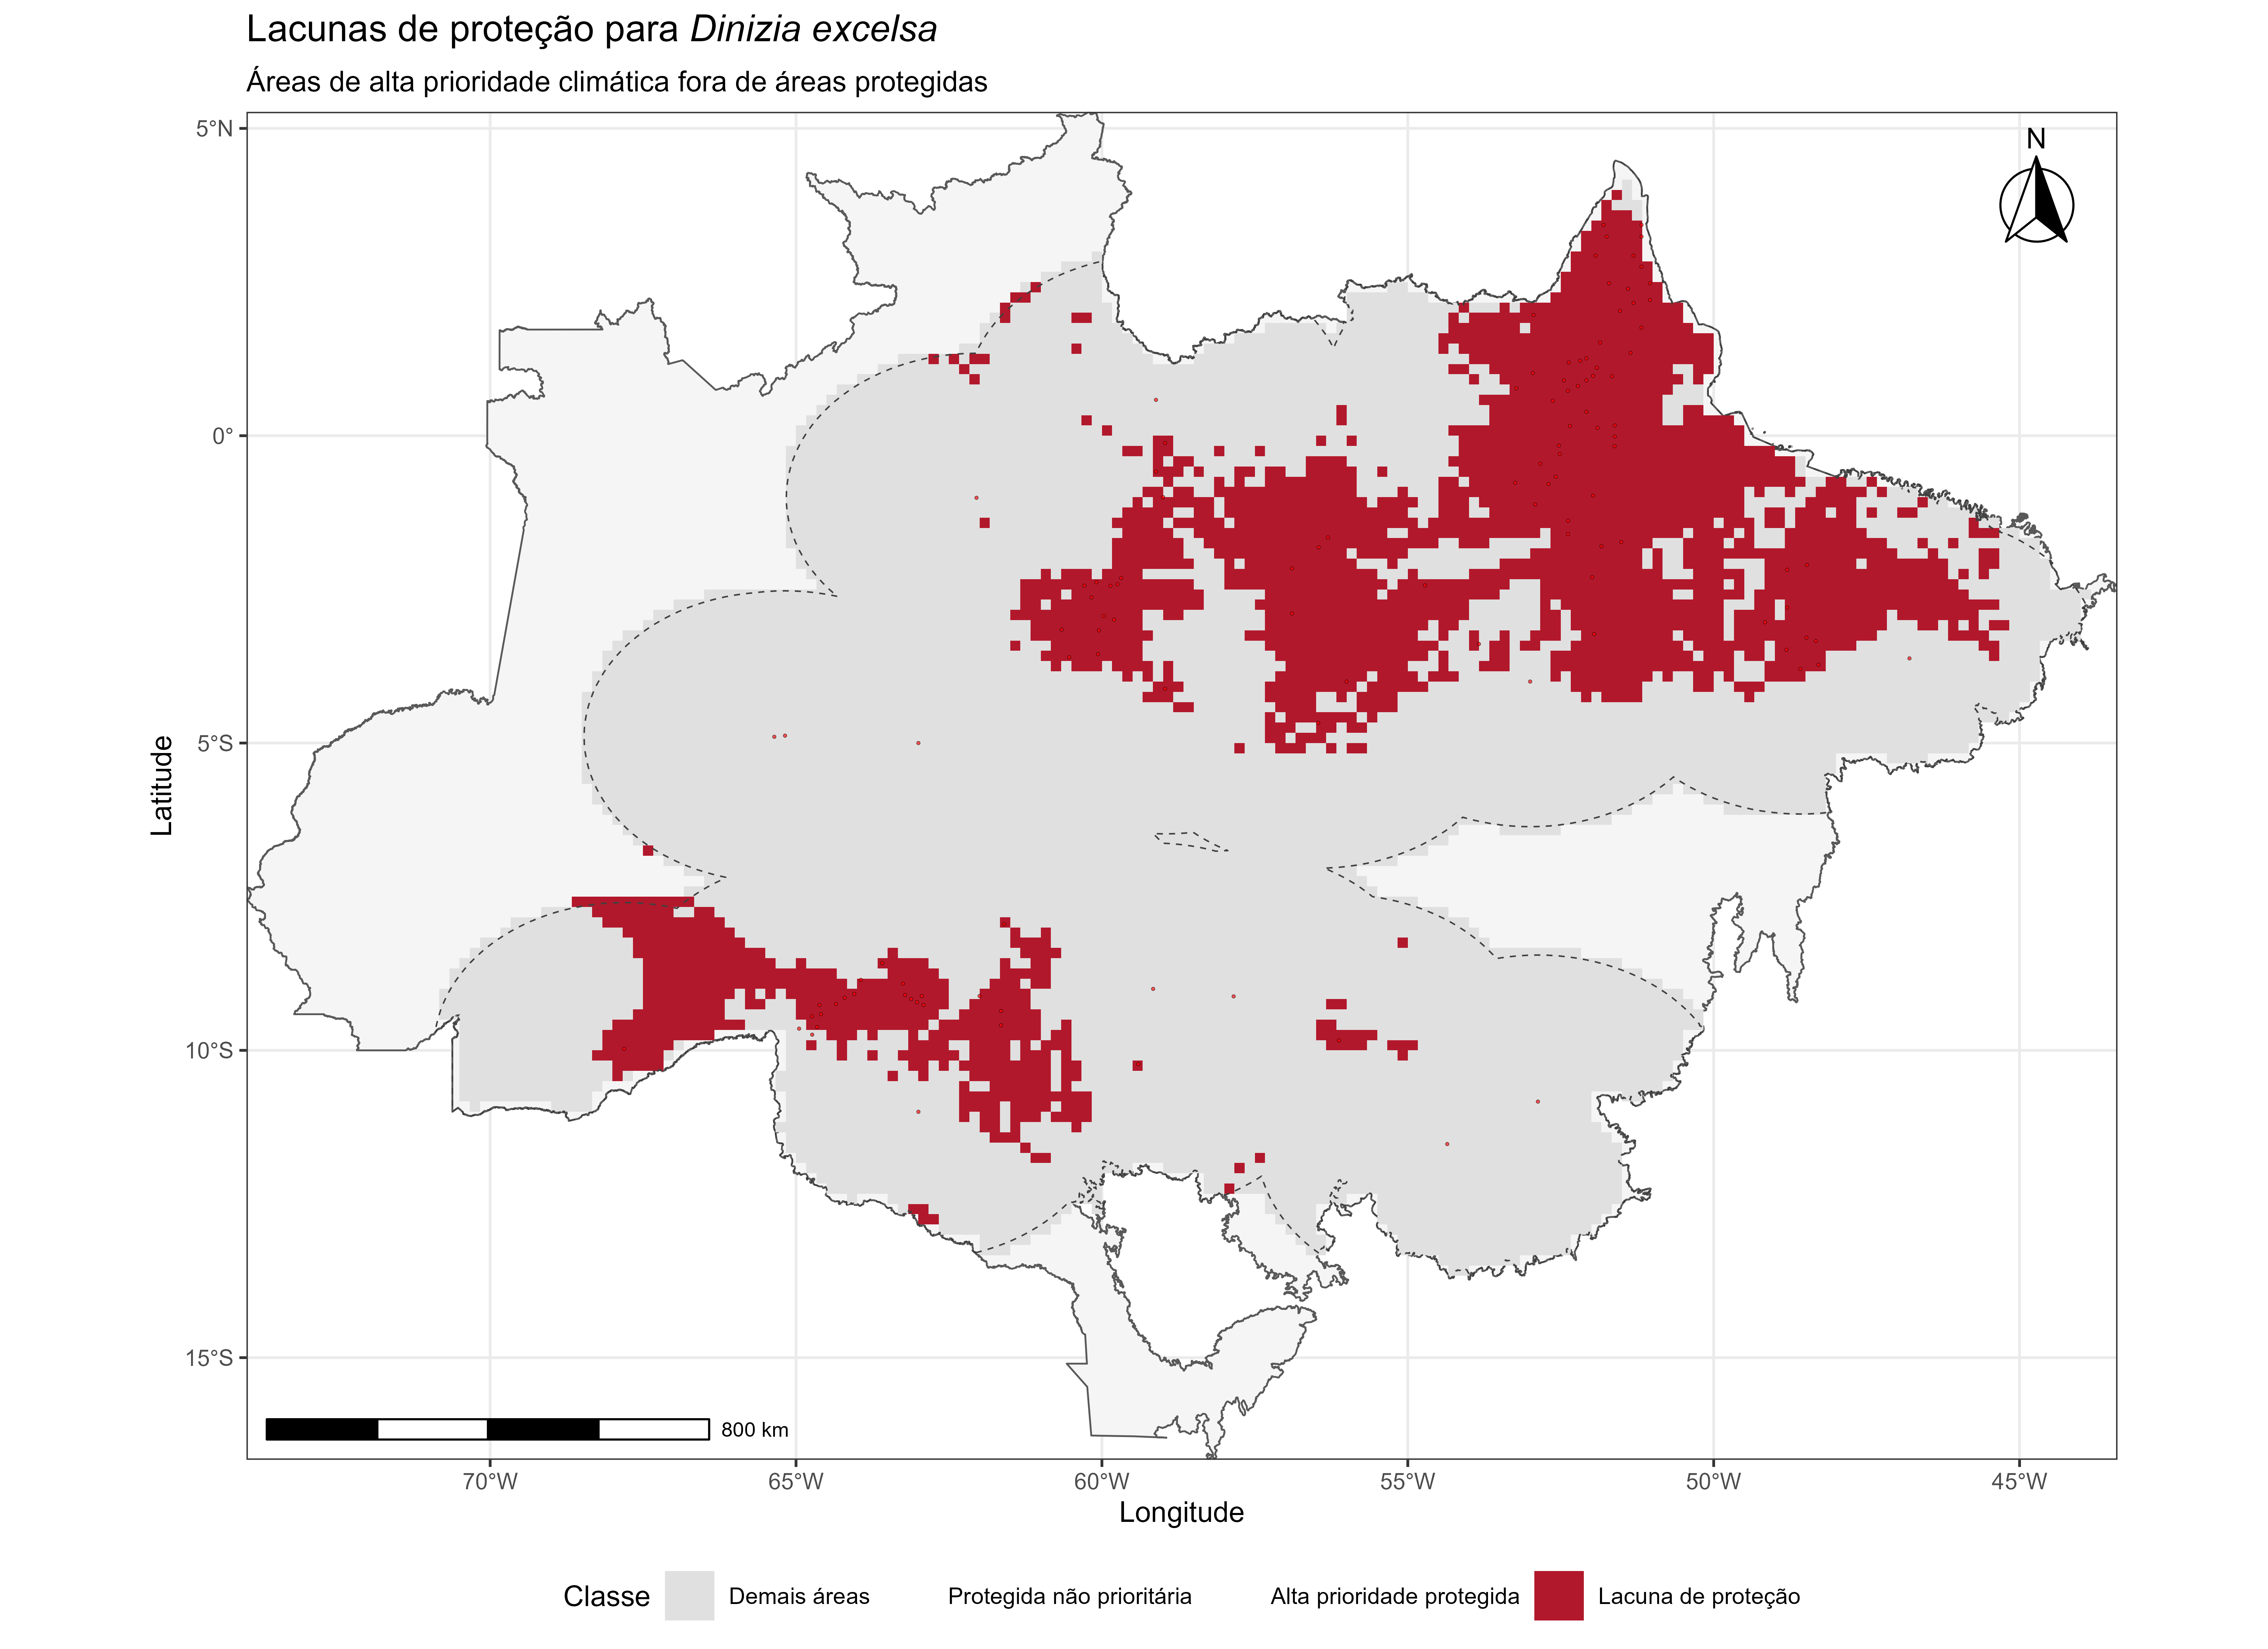
\includegraphics[width=0.90\textwidth]{figuras/unidade17/unidade17_lacunas_protecao.png}
\caption{Potential representation gaps for \textit{Dinizia excelsa}. Candidate priority areas outside the protected-area layer indicate locations requiring further assessment, not automatic proposals for designation.}
\label{fig:unidade17_lacunas}
\end{figure}

A gap analysis should report the fraction and area of each conservation feature represented within the network, ideally stratified by region, environmental class, population unit, and protection category. Nominal coverage is not equivalent to effective conservation: governance, enforcement, land tenure, degradation, and compatible management matter.

\section{An integrated priority index}

\rscriptfile{scripts/unidade17/07_prioridade_integrada_conservacao.R}

\begin{figure}[H]
\centering
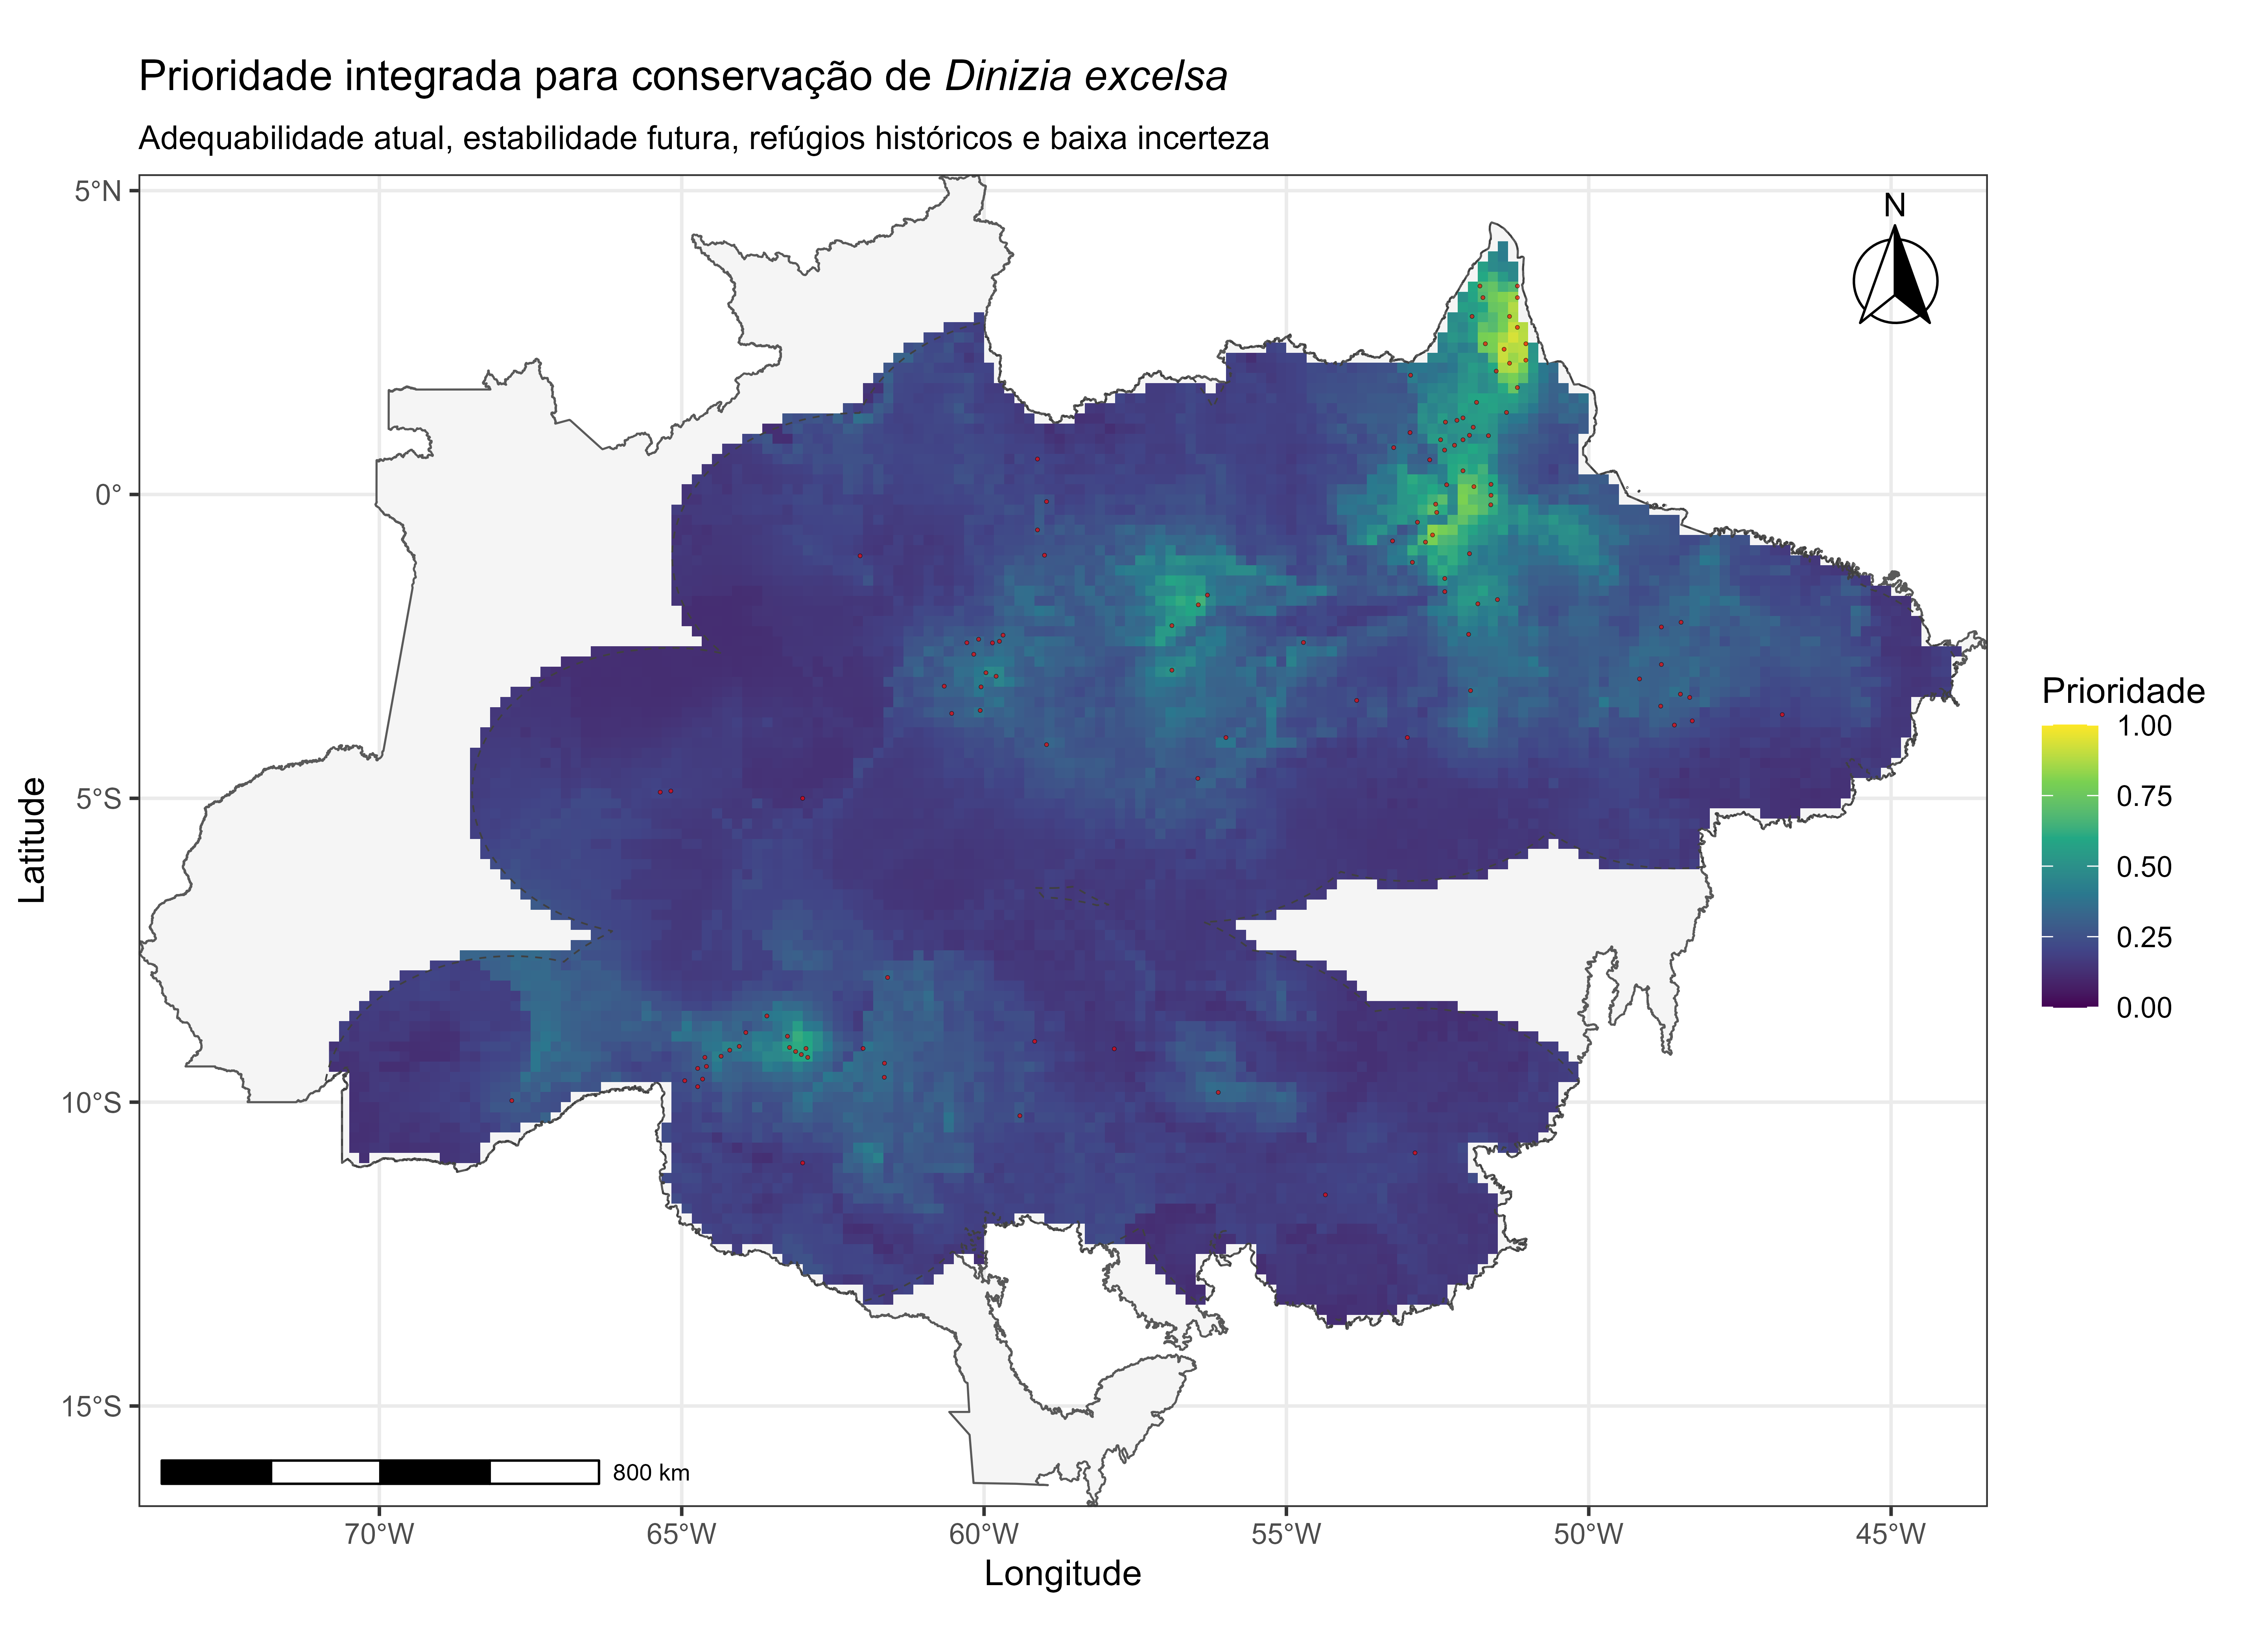
\includegraphics[width=0.90\textwidth]{figuras/unidade17/unidade17_prioridade_integrada.png}
\caption{Integrated screening index for conservation of \textit{Dinizia excelsa}.}
\label{fig:unidade17_prioridade_integrada}
\end{figure}

Weighted overlays are transparent and useful for exploration, but their results depend on normalization, weights, compensation among criteria, and classification cutoffs. A high score in one criterion may offset a critical failure in another unless veto rules are defined. Publish the formula, component layers, weights, rationale, and sensitivity analysis.

For formal systematic conservation planning, cellwise ranking should be replaced or complemented by an optimization framework that represents explicit targets while accounting for cost, complementarity, connectivity, compactness, threats, and existing commitments. Complementarity is crucial: the value of a site depends on what is already protected and on what other selected sites contribute.

\begin{atencao}[title={\faExclamationTriangle\quad A priority index is not an implementation decision}]
The index developed here is a screening tool. Designation, restoration, translocation, or assisted migration requires field verification, feasibility and risk assessment, legal review, stakeholder participation, and consideration of Indigenous Peoples and local communities.
\end{atencao}

\section{Quantitative synthesis}

\rscriptfile{scripts/unidade17/08_sintese_conservacao.R}

\begin{figure}[H]
\centering
\includegraphics[width=0.90\textwidth]{figuras/unidade17/unidade17_sintese_conservacao.png}
\caption{Quantitative summary of screening-priority classes for conservation of \textit{Dinizia excelsa}.}
\label{fig:unidade17_sintese}
\end{figure}

Report continuous scores alongside classes, because areas assigned to categories depend on arbitrary or decision-specific cutoffs. Summaries should state the geographic denominator, pixel-area correction, protected-area version, uncertainty treatment, and sensitivity to alternative criteria and weights.

\section{Complete pipeline}

\rscriptfile{scripts/unidade17/09_pipeline_conservacao.R}

\section{Chapter synthesis}

Applying SDMs to conservation requires integration of ecological modeling, climate change, uncertainty, historical stability, habitat condition, connectivity, and territorial instruments. For \textit{Dinizia excelsa}, this evidence can guide surveys, monitoring, in situ protection, restoration assessment, seed-source planning, and systematic conservation analyses. The maps identify candidates for further evaluation rather than final decisions.

\begin{conceito}[title={\faBook\quad Key message}]
The strongest conservation use of SDM is not simply to locate suitable environments. It is to support an explicit, transparent decision process that represents biodiversity features, maintains persistence and connectivity, acknowledges uncertainty, and accounts for feasibility, costs, and social legitimacy.
\end{conceito}

\section{Review exercises}

\begin{enumerate}
\item How can SDM support conservation of Amazonian tree species without being treated as a map of confirmed occurrence?
\item Why may high suitability and low model disagreement still be insufficient for prioritization?
\item Distinguish a representation gap from ineffective protection.
\item How can future projections change conservation priorities, and how should scenario disagreement be handled?
\item Why does modeled paleoclimatic stability provide only a hypothesis of refugial persistence?
\item How do complementarity and connectivity alter a cell-by-cell suitability ranking?
\item What safeguards are necessary before SDM products inform public conservation decisions?
\end{enumerate}

\section{Synthesis of the applied workflow}

The central lesson of this book is that species distribution modeling is not merely the fitting of algorithms. It is an inferential workflow connecting ecological theory, data quality, biogeographic hypotheses, environmental predictors, calibration design, statistical evaluation, spatial interpretation, transferability, uncertainty, and conservation decisions.

\begin{conceito}[title={\faBook\quad Final applied message}]
A strong SDM is not defined by a high AUC alone. It is built from fit-for-purpose data, explicit hypotheses, a justified calibration domain, ecologically defensible predictors, independently evaluated models, transparent uncertainty, and an interpretation aligned with the scientific or conservation decision.
\end{conceito}

\section{Integrative exercises}

\begin{enumerate}
\item Describe the complete workflow of an SDM project, from occurrence records to a conservation decision.
\item Why does the accessible area \(M\) influence calibration, evaluation, transfer, and conservation interpretation?
\item Compare the roles of GLM, GAM, Random Forest, BRT, and Maxent in an ensemble.
\item Why should component uncertainty and novelty maps accompany final suitability maps?
\item How can future projections support conservation while avoiding deterministic claims?
\item Which data, code, metadata, diagnostics, and decision assumptions should be delivered in a reproducible SDM project?
\item Design an SDM-based conservation study for an Amazonian species, including objectives, targets, costs, validation, uncertainty, and stakeholder participation.
\end{enumerate}


\chapter[Best practices in SDM]{Best Practices, Common Failure Modes, and Reproducibility in Species Distribution Modeling}

\markboth{Best practices in SDM}{Best practices in SDM}

\begin{objetivos}
By the end of this chapter, readers should be able to diagnose common methodological failures in SDM; connect model quality to ecological design rather than algorithm choice alone; prevent information leakage; document data provenance and analytical decisions; preserve software environments and random processes; apply FAIR principles responsibly; and prepare a transparent, auditable, and computationally reproducible SDM research package.
\end{objetivos}

\section{Introduction}

Species distribution modeling has become a central tool in ecology, biogeography, biodiversity conservation, environmental planning, and climate-change impact assessment. Its rapid expansion has been driven by new algorithms, increasingly accessible environmental data, and large occurrence repositories. These advances have also increased the need for methodological rigor, analytical transparency, and reproducibility.

SDM studies are not judged solely by algorithmic sophistication. Their credibility depends on data fitness, ecological framing, calibration design, independent evaluation, transferability, interpretation, and the availability of sufficiently documented code and data. Many failures arise not from the algorithm itself but from decisions about environmental predictors, the accessible area \(M\), sampling bias, background or pseudoabsence selection, extrapolation, and performance metrics \parencite{guisan2000predictive,elith2006novel,barve2011crucial,guisan2017habitat,zurell2020standard}.

Open science and the FAIR principles further require research objects to be identifiable, documented, accessible under clear conditions, and reusable. Openness does not mean that every sensitive coordinate or restricted dataset must be disclosed publicly; it means that access restrictions, transformations, provenance, and reproducible alternatives are documented transparently.

\section{Why do models fail?}

A common misconception is that SDMs fail primarily because the wrong algorithm was selected. Algorithms differ, but comparative work shows that data quality, ecological scope, and workflow decisions can equal or exceed algorithm choice in their effects \parencite{elith2006novel,araujo2007ensemble,guisan2017habitat}.

A model can obtain high AUC or TSS and still support an ecologically invalid interpretation. Conversely, a simple model can yield defensible inference when it is built from fit-for-purpose data, explicit hypotheses, and transparent procedures. Failure can occur at several levels:

\begin{itemize}
\item \textbf{conceptual failure}: the fitted target does not match the stated ecological question;
\item \textbf{data failure}: records or predictors are biased, erroneous, mismatched, or incomplete;
\item \textbf{design failure}: calibration, background, folds, or evaluation data do not represent deployment;
\item \textbf{statistical failure}: the model overfits, is miscalibrated, or uses an unsuitable response interpretation;
\item \textbf{transfer failure}: the model is projected beyond environmental or ecological support;
\item \textbf{communication failure}: maps and metrics are reported with stronger claims than the analysis supports.
\end{itemize}

\section{Failure mode 1: using every WorldClim variable without prior selection}

Automatically including all 19 WorldClim bioclimatic variables is rarely a neutral choice. Several variables encode overlapping temperature or precipitation summaries and may be strongly correlated. Indiscriminate inclusion can increase multicollinearity, obscure coefficient interpretation, enable overfitting, and reduce spatial or temporal transferability \parencite{dormann2013collinearity,guisan2017habitat}.

\begin{sdmwarningbox}
Large predictor sets can produce multicollinearity, unstable response functions, overfitting, low transferability, and ecologically inconsistent interpretations. More predictors do not necessarily provide more ecological information.
\end{sdmwarningbox}

Good practice combines an a priori ecological hypothesis with examination of predictor definitions, correlation, variance inflation factors, and sample-size constraints. PCA can be useful when the inferential target concerns climatic space rather than individual predictors, but it changes interpretation and must be fitted without leaking evaluation data. Predictor selection itself belongs inside each training resample when its estimates depend on the data.

\section{Failure mode 2: ignoring the accessible area \texorpdfstring{\(M\)}{M}}

The accessible area \(M\) is a central SDM design choice. In the BAM framework, observed distribution reflects the intersection of suitable abiotic conditions, biotic context, and areas historically accessible through dispersal \parencite{soberon2005interpretation,soberon2009niches,barve2011crucial}.

Sampling background or pseudoabsences from environments the species could not plausibly have encountered can confuse dispersal limitation with environmental unsuitability. The calibration extent also changes environmental availability, prevalence, discrimination metrics, fitted contrasts, and the meaning of a presence--background output.

\begin{sdmwarningbox}
An unjustified \(M\) can generate unrealistic pseudoabsences, inappropriate background, biased performance estimates, misleading response functions, and distorted projections. A larger calibration region is not automatically more conservative.
\end{sdmwarningbox}

Define \(M\) from species-specific biogeography, dispersal history, geographic barriers, hydrographic basins, ecoregions, biomes, and the temporal scale of the question. Report the rationale, source data, geometry, date, and sensitivity of results to plausible alternative delimitations.

\section{Failure mode 3: choosing a model by AUC alone}

AUC measures ranking discrimination over a specified evaluation sample. It does not establish calibration, ecological plausibility, transferability, or usefulness at a decision threshold. Its value also depends on the geographic and environmental extent from which absences or background were sampled \parencite{lobo2008auc,allouche2006assessing}.

\begin{sdmwarningbox}
Selecting the largest AUC can create false confidence, magnify negligible numerical differences, and favor a model whose response curves, calibration, or transferred predictions are ecologically implausible.
\end{sdmwarningbox}

Evaluation should match the intended use and combine spatially independent discrimination, calibration diagnostics, sensitivity and specificity when a threshold is justified, continuous-score error measures, response curves, residual or error maps, and biogeographic plausibility. Boyce-type indices may be useful in presence-only contexts but, like every metric, require a stated interpretation and appropriate data.

\section{Failure mode 4: projecting without diagnosing extrapolation}

Temporal or spatial transfer assumes that the fitted occurrence--environment relationship remains informative in the projection domain. Novel predictor values or combinations can make predictions depend primarily on the algorithm's extrapolation behavior, feature constraints, or clamping settings \parencite{elith2010functional,owens2013constraints,zurell2020standard}.

\begin{sdmwarningbox}
Transferred maps can look smooth and precise even where they are unsupported by calibration data. Without novelty diagnostics, apparent losses or gains may be artifacts of extrapolation.
\end{sdmwarningbox}

Good practice includes MESS, MOP or comparable novelty diagnostics, explicit reporting of clamping, inspection of response functions at predictor boundaries, and separate communication of projected suitability and environmental support. Novelty is not prediction error, but it identifies where stronger assumptions are operating.

\section{Failure mode 5: confusing suitability with occurrence probability}

Many SDMs produce relative suitability, relative occurrence rates, scores, or rankings. These quantities are not automatically probabilities of presence. The interpretation depends on response data, sampling design, link function, prevalence, background process, output transformation, and calibration \parencite{soberon2007grinnellian,franklin2010mapping,peterson2011ecological}.

Actual occupancy also depends on dispersal, biotic interactions, demography, disturbance, land use, detectability, and history.

\begin{sdmwarningbox}
Labeling an arbitrary suitability score as occurrence probability can overstate occupancy, misrepresent uncertainty, and turn a continuous model output into an unjustified presence--absence claim.
\end{sdmwarningbox}

Name the output according to the model and sampling design. Treat continuous maps as conditional environmental scores unless probability calibration is justified with appropriate detection, prevalence, and evaluation data. Thresholded maps must report their rule, purpose, and sensitivity.

\section{Failure mode 6: ignoring sampling bias}

Occurrence databases are rarely random samples. Records often cluster near roads, navigable rivers, cities, research institutions, protected areas, or historically surveyed regions. An untreated model may learn the geography of recording effort rather than the species' ecological association \parencite{phillips2009sample,kramer2013importance,fourcade2014mapping}.

\begin{sdmwarningbox}
Sampling bias shared by presence records and evaluation data can inflate apparent performance while leaving poorly sampled regions unsupported.
\end{sdmwarningbox}

Possible responses include coordinate validation, spatial thinning, target-group or effort-informed background, bias surfaces, occupancy or point-process approaches when their assumptions are met, and explicit mapping of data density. No correction is universally best: the treatment should reflect how records were generated and should be tested through sensitivity analysis.

\section{Failure mode 7: allowing information leakage}

Information leakage occurs when evaluation data influence model fitting or any upstream decision. Examples include selecting predictors from the complete dataset, thinning before assigning spatial folds in a way that couples folds, tuning hyperparameters on the final test data, standardizing predictors with all observations, selecting an ensemble by test performance, or repeatedly inspecting test results until the model appears satisfactory.

\begin{sdmwarningbox}
An evaluation set is no longer independent once it has guided predictor selection, preprocessing, tuning, threshold choice, algorithm inclusion, or model revision.
\end{sdmwarningbox}

All learned preprocessing and model selection should occur within training data. Nested resampling separates tuning from performance estimation. A genuinely independent dataset should be reserved for a final, pre-specified assessment whenever feasible. Spatial separation alone does not prevent leakage if duplicated records, overlapping buffers, shared raster cells, or temporally mismatched predictors connect training and test samples.

\section{From methodological quality to reproducible science}

Avoiding common errors is only part of reliable research. An ecologically defensible model can remain unverifiable when its inputs, transformations, software, and analytical decisions are undocumented. Reproducibility should therefore be designed from project inception.

\section{Reproducibility in species distribution modeling}

\subsection{Terminology and scope}

\textbf{Repeatability} concerns obtaining the same result under the same conditions. \textbf{Computational reproducibility} concerns regenerating results from the same data and code in a documented environment. \textbf{Replication} concerns testing the finding with new data, implementations, or studies. A successful rerun demonstrates computational traceability; it does not prove that the ecological inference is correct.

SDM workflows contain many linked stages: acquisition, cleaning, taxonomic decisions, spatial filtering, predictor processing, definition of \(M\), background generation, model fitting, validation, climate transfer, uncertainty analysis, and visualization. Small changes in software versions, defaults, random seeds, grids, or source datasets can alter outputs. International journals and open-science initiatives therefore recommend transparent computational documentation \parencite{wilkinson2016fair,peng2011reproducible,sandve2013ten,zurell2020standard}.

\subsection{A project as a dependency graph}

A reproducible workflow should be executable from immutable raw inputs to final tables and figures. Scripts should declare inputs and outputs, avoid hidden manual steps, use project-relative paths, and fail clearly when prerequisites are absent. Workflow tools can track dependencies and rerun only outdated products, but even a numbered script pipeline is useful when ordering and contracts are explicit.

Raw data should be read-only. Cleaning and harmonization must create derived files, accompanied by machine-readable logs or tables recording exclusions, coordinate changes, taxonomic reconciliation, duplicate rules, units, and spatial transformations. Large intermediates need not all be archived if they can be regenerated reliably.

\subsection{Controlling the computational environment}

Record the operating system, R version, locale, relevant system libraries, package versions, and external software. In R, basic session metadata can be captured with:

\begin{rcode}
sessionInfo()
\end{rcode}

For fuller provenance, save this output automatically at the end of a successful pipeline and record the version or commit of the analysis code. Random seeds should be set and documented for stochastic operations, while parallel random-number generation requires a reproducible stream rather than a single informal seed.

\begin{sdmpracticebox}
Archive session metadata, random-seed policy, configuration files, and a machine-readable manifest with the analysis outputs. A manuscript statement alone is not sufficient to reconstruct the environment.
\end{sdmpracticebox}

\subsection{Managing dependencies}

Package updates can change functions, defaults, dependencies, and numerical behavior. The R package \texttt{renv} records project dependencies in a lockfile:

\begin{rcode}
renv::snapshot()
\end{rcode}

Another researcher can request the recorded package set with:

\begin{rcode}
renv::restore()
\end{rcode}

A lockfile improves reproducibility but does not guarantee it indefinitely: packages may require system libraries, archived binaries may disappear, and external web services can change. Containers or archived computational environments can add protection for long-lived projects. Always test restoration in a clean environment before publication.

\subsection{Version control with Git}

Version control records changes to code, documentation, and small configuration files. A repository can be initialized with:

\begin{shellcode}
git init
git add .
git commit -m "Initial reproducible workflow"
\end{shellcode}

Useful practices include small meaningful commits, reviewed branches, tagged releases, issue tracking, and a changelog for published versions. Generated outputs, secrets, credentials, personal information, and very large binary files should not be committed indiscriminately. A public repository is a collaboration platform; an archived release with a persistent identifier is the citable research object.

\subsection{Sharing data, code, and metadata}

Data and code should be shared whenever legally, ethically, and scientifically appropriate. Sensitive species coordinates may need generalization, controlled access, or an embargo. Third-party licenses can prevent redistribution even when analysis code is open. In those cases, provide accession identifiers, acquisition instructions, checksums where permitted, schemas, and a synthetic or reduced dataset that exercises the workflow.

\begin{table}[H]
\centering
\caption{Common platforms used to develop, archive, and share scientific research objects.}
\label{tab:repositorios_ciencia_aberta}
\begin{tabular}{p{0.20\textwidth}p{0.70\textwidth}}
\toprule
\textbf{Platform} & \textbf{Principal role} \\
\midrule
GitHub & Version control, documentation, issue tracking, and collaborative code development. \\
Zenodo & Preservation of versioned research objects and assignment of persistent DOIs. \\
Dryad & Curated publication and preservation of research datasets. \\
Figshare & Publication of datasets, figures, tables, and supplementary materials. \\
\bottomrule
\end{tabular}
\end{table}

A common workflow develops the project in a version-control platform and archives a tagged release in a preservation repository. Cite the archived version and record the repository URL, release tag, commit identifier, license, and DOI in the manuscript.

\subsection{FAIR principles}

The FAIR principles provide guidance for making digital research objects Findable, Accessible, Interoperable, and Reusable \parencite{wilkinson2016fair}.

\begin{table}[H]
\centering
\caption{FAIR principles for scientific data and research objects.}
\label{tab:fair_principles}
\begin{tabular}{p{0.15\textwidth}p{0.75\textwidth}}
\toprule
\textbf{Principle} & \textbf{Practical interpretation} \\
\midrule
Findable & Assign persistent identifiers and rich, searchable metadata. \\
Accessible & Use standardized retrieval protocols and clearly state authentication or restriction conditions. \\
Interoperable & Use documented formats, vocabularies, units, coordinate systems, and machine-readable schemas. \\
Reusable & Provide provenance, licenses, variable definitions, quality information, and sufficient contextual documentation. \\
\bottomrule
\end{tabular}
\end{table}

FAIR is not synonymous with unrestricted openness. A protected dataset can remain FAIR when its metadata are findable and its access conditions are explicit. Conversely, placing undocumented files online does not make them reusable.

\subsection{Minimum reporting for an SDM study}

A publication-ready report should identify:

\begin{itemize}
\item the ecological question, response interpretation, target population, spatial domain, period, and intended deployment;
\item occurrence sources, download dates, licenses, taxonomic treatment, cleaning rules, duplicate handling, temporal filters, and sample sizes at every stage;
\item the definition and rationale for \(M\), background or pseudoabsence design, bias treatment, and sensitivity analyses;
\item predictor sources, versions, units, temporal baselines, resolution, resampling, selection procedure, and ecological rationale;
\item algorithms, packages, versions, hyperparameter search spaces, tuning criteria, seeds, fitted settings, and convergence or diagnostic checks;
\item validation design, fold construction, buffers, independence safeguards, metrics, thresholds, calibration assessment, and uncertainty intervals;
\item projection GCMs, SSPs, periods, downscaling products, clamping settings, dispersal assumptions, and novelty diagnostics;
\item ensemble inclusion and weighting rules, uncertainty components, aggregation formulas, and decision thresholds;
\item code and data availability, persistent identifiers, licenses, access restrictions, environment lockfile, and instructions for end-to-end execution.
\end{itemize}

Tables of exclusions and workflow manifests are often more auditable than prose alone. Report deviations from a pre-specified protocol and distinguish exploratory analyses from confirmatory evaluation.

\subsection{Reproducibility checklist}

Before submission, verify that:

\begin{itemize}
\item scripts regenerate every reported table, figure, and numerical result from documented inputs;
\item raw data are immutable and every transformation is traceable;
\item software and package versions, seeds, locale, and system dependencies are recorded;
\item a clean restoration of the environment and pipeline has been tested;
\item data and code have licenses, metadata, checksums or persistent identifiers where appropriate;
\item sensitive or licensed data have explicit access conditions and a reproducible substitute when feasible;
\item training, tuning, and evaluation information are separated without leakage;
\item all manual GIS or editorial operations are scripted or documented precisely;
\item figures carry units, coordinate information, legends, scenario identifiers, and uncertainty or novelty context;
\item FAIR principles and long-term preservation have been considered.
\end{itemize}

\begin{sdmkeybox}
Computational reproducibility is achieved when a documented research package can regenerate the reported results in a reconstructed environment. Scientific credibility additionally requires valid data, defensible assumptions, appropriate evaluation, and independent scrutiny.
\end{sdmkeybox}

\section{Summary of common failures and recommended practices}

\begin{table}[H]
\centering
\caption{Common SDM failure modes, consequences, and recommended practices.}
\label{tab:erros_comuns_sdm}
\scriptsize
\setlength{\tabcolsep}{3pt}
\begin{tabular}{p{0.24\textwidth}p{0.33\textwidth}p{0.34\textwidth}}
\toprule
\textbf{Failure mode} & \textbf{Potential consequence} & \textbf{Recommended practice} \\
\midrule
Use every available climate predictor & Collinearity, overfitting, unstable transfer, and weak interpretation & Define ecological hypotheses; examine redundancy; select within training resamples \\
Ignore accessible area \(M\) & Inappropriate background, biased contrasts, and misleading performance & Justify \(M\) biogeographically and assess sensitivity to alternatives \\
Select a model by AUC alone & False confidence and poor calibration or ecological plausibility & Match metrics to use; assess calibration, spatial transfer, response curves, and errors \\
Transfer without novelty diagnostics & Unsupported predictions and artificial gains or losses & Report MESS, MOP or comparable diagnostics and clamping behavior \\
Call suitability an occurrence probability & Overstated occupancy and unjustified binary maps & Name outputs according to model and sampling design; calibrate only when justified \\
Ignore sampling bias & Model collection effort rather than species--environment association & Diagnose effort; use justified thinning, bias-aware background, or observation models \\
Leak evaluation information & Optimistically biased performance and model-selection results & Nest preprocessing and tuning within training data; reserve independent evaluation \\
\bottomrule
\end{tabular}
\end{table}

\section{Chapter synthesis}

SDM quality depends on the complete chain of evidence, not only on the fitted algorithm. Ecological scope, occurrence provenance, accessible area, predictors, sampling process, validation, extrapolation, output interpretation, and uncertainty all affect the conclusion. Reproducibility adds the infrastructure required to inspect and regenerate that chain: versioned code, documented data, controlled dependencies, persistent archives, metadata, and executable workflows.

Modern distribution modeling should produce more than attractive suitability maps. It should create transparent, verifiable, reusable evidence whose limitations are visible and whose claims remain aligned with the data and deployment context.

\begin{sdmkeybox}
A simple, ecologically grounded, independently evaluated, and fully documented model can be more trustworthy than a complex model built with redundant predictors, an unjustified calibration domain, untreated bias, leaked evaluation data, and performance claims based on a single metric.
\end{sdmkeybox}

\section{Review exercises}

\begin{enumerate}
\item Explain why algorithm choice is only one component of SDM quality.
\item Design a leakage-free workflow for predictor selection, tuning, ensemble construction, and final evaluation.
\item Distinguish computational reproducibility from independent replication.
\item What information is required to make a restricted occurrence dataset FAIR without publishing sensitive coordinates?
\item Why does an \texttt{renv.lock} file improve, but not guarantee, long-term reproducibility?
\item Construct a minimum reporting checklist for a future climate projection.
\item Audit one chapter workflow in this book and identify every input, transformation, random process, and output that should be recorded in a provenance manifest.
\end{enumerate}

\chapter[Final considerations]{Final Considerations}

\begin{objetivos}
By the end of this chapter, readers should be able to view species distribution modeling as an integrative field spanning ecology, biogeography, statistics, spatial data science, climate change, and conservation; synthesize the principal methodological decisions developed throughout the book; evaluate the capabilities and limitations of SDMs; and formulate responsible ecological interpretations from spatial models.
\end{objetivos}

\section{Synthesis of the book}

This book presents species distribution modeling in R as a complete, critical, and reproducible scientific workflow. It begins with ecological-niche theory and progresses through occurrence data, environmental predictors, multicollinearity, accessible-area and background design, statistical and machine-learning algorithms, presence--background modeling, ensembles, evaluation, future projections, paleoclimate, extrapolation, uncertainty, conservation, and reproducible research.

The case study of \textit{Dinizia excelsa} demonstrates that an SDM is not simply a technique for producing an environmental-suitability map. It is a chain of inference linking ecological hypotheses, spatial data, niche theory, sampling processes, methodological choices, statistical evaluation, geographic transfer, and biogeographic interpretation.

\begin{conceito}[title={\faBook\quad Central message}]
A strong SDM is not defined by an attractive map or a single performance metric. It depends on alignment among the ecological question, data-generating process, accessible area, predictors, model complexity, independent evaluation, transferability, uncertainty, and the intended interpretation or decision.
\end{conceito}

\section{From ecological niche to geographic space}

Species distributions are not determined by climate alone. Occurrence reflects abiotic conditions, biotic interactions, historical accessibility, dispersal, demographic processes, disturbance, and evolutionary history. The BAM framework emphasizes that observed distribution is only one outcome of these interacting constraints and that \(M\) influences the contrasts learned during calibration.

The distinction between environmental and geographic space is fundamental. Models learn associations from samples embedded in environmental space and then map those associations geographically. Spatial patterns may reflect ecological mechanisms, environmental availability, autocorrelation, sampling effort, or the geometry of the study region. Interpretation must therefore return to the original question and the deployment domain.

\section{Occurrence data and analytical responsibility}

Occurrence records from inventories, herbaria, public databases, and platforms such as GBIF are scientifically valuable but imperfect. Taxonomic errors, imprecise coordinates, duplicates, temporal mismatch, raster-cell duplication, and spatial sampling bias can affect every subsequent result.

Data cleaning is consequently part of inference, not clerical preparation. Taxonomic verification, coordinate diagnostics, transparent exclusions, spatial thinning where justified, effort assessment, and a complete attrition record improve credibility. Cleaning rules must not be optimized against the final evaluation outcome.

\begin{atencao}[title={\faExclamationTriangle\quad Data quality precedes model complexity}]
No algorithm compensates for unsuitable data, an unjustified accessible area, or incoherent predictors. In SDM, inferential quality is determined before as well as during model fitting.
\end{atencao}

\section{Environmental predictors and ecological interpretation}

Predictors connect species ecology to model structure, but a statistically important variable is not automatically a causal mechanism. It may represent a relevant environmental gradient, act as a proxy for an unmeasured driver, share information with correlated predictors, or encode the geography of sampling.

Predictor choice should combine ecological hypotheses, scale, data support, redundancy, and transfer requirements. Correlation, VIF, and PCA answer different questions. Parsimony is valuable when it improves interpretability and transferability, but arbitrary removal can omit important dimensions. Any data-dependent selection must be nested within training resamples.

\section{Algorithms as operational hypotheses}

GLM, GAM, Random Forest, BRT, and Maxent represent different ways to estimate occurrence--environment relationships. GLMs emphasize a specified response form; GAMs estimate penalized smooth responses; Random Forest and BRT capture nonlinearities and interactions through tree ensembles; and Maxent-type methods estimate relative occurrence or suitability from presence and background data.

No algorithm is universally superior. Complexity can improve flexibility while increasing sensitivity to tuning, sample size, and extrapolation. Comparison should therefore include discrimination, calibration where meaningful, response behavior, spatial error, stability, novelty, and transfer performance.

\begin{conceito}[title={\faBook\quad Algorithms as operational hypotheses}]
Each algorithm encodes assumptions about how the observed response relates to the environment. Comparing algorithms evaluates the robustness of conclusions to model structure; it should not become an automatic search for the largest AUC.
\end{conceito}

\section{Evaluation, thresholds, and binary maps}

No single metric provides a complete evaluation. AUC measures ranking discrimination; TSS and confusion-matrix measures depend on a threshold and evaluation design; the Brier score concerns squared probabilistic error when predictions have a probability interpretation; calibration addresses agreement between predicted and observed frequencies; and presence-only measures have their own sampling assumptions.

Continuous predictions may be thresholded to summarize potential area, stability, loss, gain, or representation. These categories inherit the threshold's assumptions and uncertainty. Binary maps are analytical and decision tools, not definitive maps of species presence and absence. Spatially structured or genuinely independent evaluation is normally more relevant to geographic transfer than random partitions.

\section{Future projections and climate change}

Future SDM projections explore conditional changes under specified GCMs, SSPs, periods, and model assumptions. SSP-based pathways are not deterministic forecasts. A future map should be read as an if--then statement: if the fitted association remains informative, if the stated climate trajectory and GCM are realized, and if omitted ecological processes do not overturn the response, then environmental suitability may change in the mapped direction.

Uncertainty arises from present data, algorithms, calibration, GCMs, downscaling, pathways, periods, land-use assumptions, dispersal, and extrapolation. Reporting only an ensemble mean conceals this hierarchy.

\section{Paleoclimate and biogeographic history}

Paleoclimate transfer connects contemporary climatic associations with reconstructed conditions during the mid-Holocene, Last Glacial Maximum, or Last Interglacial. It can identify candidates for climatic stability and generate hypotheses about historical connectivity or persistence.

Paleoclimate projections do not demonstrate past occurrence or refugia. Such claims require independent evidence from paleoecology, fossils, phylogeography, population genetics, or demography. Variation among different time periods is an ecological temporal signal; uncertainty within a time slice should be assessed across plausible reconstructions and modeling choices.

\section{Transfer, extrapolation, and evidential support}

Spatial and temporal transfer can encounter environmental values or multivariate combinations absent from calibration. MESS, MOP, and related methods diagnose environmental novelty; they do not directly estimate prediction error. High agreement among algorithms is not strong evidence when every algorithm is extrapolating in the same unsupported region.

\begin{atencao}[title={\faExclamationTriangle\quad High suitability is not high confidence}]
A cell may receive a high suitability score while exhibiting strong environmental novelty, scenario disagreement, or sensitivity to model structure. Suitability and evidential support must be communicated separately.
\end{atencao}

Uncertainty components should retain their distinct meanings. Algorithmic disagreement, scenario sensitivity, climate-model spread, sampling variation, and novelty cannot be added as if they were automatically commensurable variances. An integrated caution index is useful only when its transformations, weights, dependencies, and sensitivity are explicit.

\section{Conservation applications}

In conservation, SDMs are evidence layers rather than final answers. Spatial planning may combine modeled suitability, future persistence, candidate historical stability, habitat condition, connectivity, threats, protected-area representation, costs, feasibility, uncertainty, and field knowledge.

For an Amazonian tree such as \textit{Dinizia excelsa}, these products can guide surveys, monitoring, restoration assessment, seed-source planning, protection-gap analysis, and systematic conservation planning. Decisions additionally require legal and social analysis, stakeholder participation, and respect for the rights and knowledge of Indigenous Peoples and local communities.

\section{Principles for defensible SDM studies}

\begin{enumerate}
\item Define the ecological question, target response, domain, period, and intended deployment before modeling.
\item Audit taxonomy, coordinates, sampling effort, temporal compatibility, and record provenance.
\item Define and justify the accessible area \(M\).
\item Select predictors using ecological rationale, scale, support, and transfer objectives.
\item Address redundancy and multicollinearity without leaking evaluation information.
\item Compare model structures and complexity using pre-specified tuning rules.
\item Separate training, tuning, and independent evaluation spatially and analytically.
\item Interpret metrics together with calibration, maps, response curves, and spatial errors.
\item Diagnose novelty and disclose clamping in every spatial or temporal transfer.
\item Preserve distinct sources of uncertainty and evaluate sensitivity to analytical choices.
\item Make code, provenance, dependencies, metadata, and decisions reproducible under appropriate access conditions.
\item Align claims with the model output and communicate limitations plainly.
\end{enumerate}

\section{Limitations and future directions}

SDMs remain simplifications of ecological reality. Dispersal, demography, biotic interactions, human disturbance, land-use change, phenotypic plasticity, local adaptation, and evolutionary change are often absent or represented indirectly.

Promising directions include integration with demographic and dynamic range models, genomics, traits, LiDAR and other remote sensing, permanent forest inventories, joint species models, connectivity, deforestation scenarios, causal designs, and systematic conservation planning. For Amazonia, these integrations are urgent under interacting climate change, fragmentation, fire, extraction, and biodiversity loss. Methodological novelty should remain subordinate to a clear ecological question and verifiable evidence.

\section{Final message}

Species distribution modeling transforms dispersed occurrence and environmental observations into spatial hypotheses for research, teaching, and conservation. Its strength lies not in an algorithm alone but in the coherence and transparency of the full scientific process.

\begin{conceito}[title={\faLeaf\quad Final reflection}]
Modeling a species distribution is an attempt to understand how life occupies space under environmental, historical, and dispersal constraints. In a changing world, carefully designed SDMs can reveal risk, identify testable conservation opportunities, and support more responsible decisions---provided that uncertainty and limits remain visible.
\end{conceito}

\chapter{Glossary}

\section*{How to use this glossary}

This glossary provides concise definitions of recurring terms from ecology, biogeography, climatology, statistics, spatial data science, and reproducible computing. Definitions describe how the terms are used in this book; readers should consult the cited specialist literature for formal treatments and implementation-specific meanings.

\begin{longtable}{p{0.20\textwidth}p{0.70\textwidth}}
\caption{Glossary of principal terms used in species distribution modeling.}
\label{tab:glossario_sdm}\\
\toprule
\textbf{Term} & \textbf{Definition} \\
\midrule
\endfirsthead
\toprule
\textbf{Term} & \textbf{Definition} \\
\midrule
\endhead
Accessible area (\(M\)) & Geographic region hypothesized to have been reachable by the species over the relevant historical and dispersal period; it defines the environmental availability used for calibration. \\
Algorithmic disagreement & Variation among predictions from different fitted algorithms under otherwise comparable data and design; it is descriptive and is not automatically a confidence interval. \\
AUC & Area under the receiver operating characteristic curve; a threshold-independent measure of ranking discrimination for a specified evaluation sample. \\
Background & Sample representing environmental availability in the calibration domain for presence--background methods; background points are not observed absences. \\
BAM framework & Conceptual framework relating distribution to biotic conditions (B), abiotic conditions (A), and movement or accessibility (M). \\
Boyce index & Presence-only evaluation index comparing the frequency of observed presences with the availability of prediction classes; interpretation depends on implementation and sampling design. \\
Brier score & Mean squared difference between a binary outcome and a probabilistic prediction; meaningful as a calibration-sensitive score only when predictions have a probability interpretation. \\
BRT & Boosted Regression Trees; an ensemble of sequentially fitted trees in which later trees improve residual predictive structure. \\
Calibration & Agreement between predicted probabilities and observed event frequencies, or, more broadly in SDM usage, the process of fitting a model. The intended meaning should be stated. \\
CHELSA & High-resolution climatology product using statistical downscaling informed by atmospheric and topographic processes. \\
Clamping & Constraining predictor values or model responses during transfer to reduce behavior beyond the calibration range; settings and affected areas should be reported. \\
CMIP6 & Coupled Model Intercomparison Project Phase 6, which coordinates simulations from multiple global climate models. \\
Computational reproducibility & Ability to regenerate reported results from the same data, code, and a documented computational environment. \\
Cross-validation & Resampling procedure that repeatedly partitions data into training and assessment sets; spatial or environmental partitions may better represent geographic transfer than random folds. \\
DOI & Digital Object Identifier; a persistent identifier commonly assigned to publications, datasets, software releases, and other research objects. \\
Ecological niche & Multidimensional set of conditions and resources associated with population persistence, interpreted within a specified conceptual framework and scale. \\
ENM & Ecological niche model; a model intended to characterize aspects of a species' niche, often projected geographically. The term should not be treated as interchangeable with every SDM without qualification. \\
Ensemble & Combination or synthesis of predictions from multiple fitted models. It represents between-model consensus or spread but does not remove shared bias. \\
Environmental novelty & Degree to which a projection environment differs from the environmental domain represented during calibration. \\
Environmental suitability & Model-derived compatibility between environmental conditions and the estimated occurrence--environment association; not automatically probability of presence or habitat quality. \\
Extrapolation & Application of a model to predictor values or multivariate combinations outside those represented during calibration. \\
FAIR & Principles according to which digital research objects should be Findable, Accessible, Interoperable, and Reusable. FAIR does not require unrestricted public access. \\
Fundamental niche & Conditions under which a species could maintain populations in the absence of constraining biotic interactions, subject to physiological, resource, demographic, and scale assumptions. \\
GAM & Generalized Additive Model; an extension of generalized linear modeling that estimates penalized smooth predictor effects. \\
GCM & Global Climate Model or General Circulation Model; a numerical representation of the climate system used to simulate past, present, and future conditions. \\
Git & Distributed version-control system used to record and manage changes to code and text. \\
GitHub & Online platform providing Git repository hosting and collaboration services; it is not, by itself, a permanent scientific archive. \\
GLM & Generalized Linear Model; a model relating a response distribution to a linear predictor through a link function. \\
HSM & Habitat Suitability Model; a model intended to estimate habitat suitability, which may include climate, resources, structure, and other habitat attributes. \\
Kappa & Chance-corrected agreement statistic sometimes applied to thresholded predictions; it is sensitive to prevalence and marginal frequencies. \\
Last Glacial Maximum (LGM) & Climatic interval around 21 thousand years before present commonly used in paleoclimate projection studies. \\
Last Interglacial (LIG) & Warm interval commonly represented by climate products around 120--130 thousand years before present. \\
Maxent & Maximum-entropy or equivalent presence--background modeling approach used to estimate relative occurrence or suitability from features and regularization. Its common logistic output is not automatically absolute occurrence probability. \\
MESS & Multivariate Environmental Similarity Surface; diagnostic that identifies univariate range departures and summarizes similarity relative to a calibration reference. \\
Mid-Holocene & Paleoclimatic time slice approximately 6 thousand years before present. \\
MOP & Mobility-Oriented Parity; environmental-space diagnostic designed to identify strict extrapolation and similarity between calibration and projection domains. Scale direction depends on implementation. \\
Nested resampling & Evaluation design in which an inner resampling loop performs tuning or selection and an outer loop estimates generalization performance. \\
PCA & Principal Component Analysis; linear transformation that represents correlated variables using orthogonal components ordered by explained variance. \\
Presence--absence data & Observations with surveyed presences and nondetections or absences whose interpretation depends on survey and detection design. \\
Presence--background data & Observed presence records contrasted with a sample of available environments; the background does not establish absence. \\
Pseudoabsence & Location treated as an absence for fitting or evaluation despite the absence of confirmed nondetection evidence; generation rules affect the fitted target. \\
Random Forest (RF) & Ensemble of randomized decision trees whose predictions are aggregated across trees. \\
Realized niche & Portion of niche-related conditions expressed under biotic interactions, accessibility, demography, disturbance, and the observed environmental domain; it is not simply the geographic occupied area. \\
ROC curve & Receiver operating characteristic curve plotting sensitivity against the false-positive rate across thresholds. \\
SDM & Species Distribution Model; a model relating species observations to environmental or spatial predictors to estimate distribution-related quantities in a defined domain. \\
Spatial sorting bias & Inflation of evaluation performance when test sites are environmentally or geographically closer to training presences than to training absences or background. \\
SSP & Shared Socioeconomic Pathway; a socioeconomic development narrative that, when combined with climate-policy and forcing assumptions, supports conditional climate projections. \\
SSP1--2.6 & Sustainability-oriented pathway associated with an approximate forcing level of 2.6 W\,m\(^{-2}\) by 2100. \\
SSP5--8.5 & Fossil-fuel-intensive pathway associated with an approximate forcing level of 8.5 W\,m\(^{-2}\) by 2100. \\
Transferability & Ability of a fitted model to provide useful predictions in a new region, period, population, or environmental domain relevant to deployment. \\
TSS & True Skill Statistic, calculated as sensitivity plus specificity minus one for a specified threshold and evaluation sample. \\
Uncertainty & Incomplete knowledge about an estimate, process, or outcome; distinct from systematic bias, environmental novelty, and deliberate variation among scenarios. \\
VIF & Variance Inflation Factor; measure of how much variance of a regression coefficient is inflated by linear dependence among predictors. \\
WorldClim & Global gridded climate dataset widely used for baseline and projected bioclimatic variables. \\
Zenodo & General-purpose research repository that archives releases and can assign DOIs. \\
\bottomrule
\end{longtable}

\begin{conceito}[title={\faBook\quad Terminology evolves}]
SDM terminology continues to evolve, and the same term can carry different meanings across ecological, statistical, and software communities. Authors should define the modeled response, sampling design, output scale, and deployment domain rather than rely on labels alone.
\end{conceito}

\chapter{Essential Reading}

\section*{How to use this guide}

The literature on species distribution modeling has expanded across ecological theory, statistics, spatial data science, climate impacts, and conservation. The works below provide entry points rather than an exhaustive bibliography. Readers should use the complete reference list for full bibliographic details and should follow citation networks to newer evaluations and domain-specific applications.

\section{Foundational books}

\begin{table}[H]
\centering
\caption{Recommended books and extended resources for deeper study of SDM.}
\label{tab:livros_sdm}
\small
\setlength{\tabcolsep}{3pt}
\begin{tabular}{p{0.30\textwidth}p{0.24\textwidth}p{0.36\textwidth}}
\toprule
\textbf{Work} & \textbf{Author(s)} & \textbf{Principal contribution} \\
\midrule
\textit{Mapping Species Distributions} & Franklin (2010) & Ecological, statistical, and spatial foundations of species distribution modeling. \\
\textit{Habitat Suitability and Distribution Models} & Guisan, Thuiller, and Zimmermann (2017) & Comprehensive treatment of theory, workflow design, algorithms, evaluation, and applications. \\
\textit{Ecological Niches and Geographic Distributions} & Peterson et al. (2011) & Conceptual foundations connecting ecological niches, geography, and model interpretation. \\
\textit{Species Distribution Modeling with R} & Hijmans and Elith & Practical instructional material for implementing distribution-model workflows in R; readers should verify the version and accompanying software. \\
\textit{Biogeography} & Lomolino et al. & Broad biogeographic foundations needed to interpret spatial ecological patterns. \\
\bottomrule
\end{tabular}
\end{table}

\section{Foundational articles}

\begin{table}[H]
\centering
\caption{Selected articles illustrating major conceptual and methodological developments in SDM.}
\label{tab:artigos_classicos_sdm}
\small
\setlength{\tabcolsep}{3pt}
\begin{tabular}{p{0.29\textwidth}p{0.14\textwidth}p{0.43\textwidth}}
\toprule
\textbf{Reference} & \textbf{Year} & \textbf{Principal contribution} \\
\midrule
Guisan and Zimmermann & 2000 & Early synthesis of predictive habitat and species-distribution modeling. \\
Soberón and Peterson & 2005 & Conceptual linkage among ecological niche, accessibility, and geographic distribution. \\
Phillips, Anderson, and Schapire & 2006 & Formal introduction of maximum-entropy modeling for species geographic distributions. \\
Elith et al. & 2006 & Broad comparison of contemporary distribution-modeling methods. \\
Araújo and New & 2007 & Foundations and rationale for ensemble forecasting. \\
Elith, Kearney, and Phillips & 2010 & Examination of model behavior under environmental extrapolation. \\
Barve et al. & 2011 & Importance of the accessible area in model calibration and evaluation. \\
Zurell et al. & 2020 & Standardized reporting protocol for species distribution models. \\
\bottomrule
\end{tabular}
\end{table}

\section{Evaluation, transferability, and uncertainty}

\begin{itemize}
\item Fielding and Bell (1997)---assessment strategies for presence--absence prediction models.
\item Allouche, Tsoar, and Kadmon (2006)---evaluation of prevalence-sensitive and threshold-dependent measures.
\item Lobo, Jiménez-Valverde, and Real (2008)---limitations of AUC as a general measure of model performance.
\item Roberts et al. (2017)---cross-validation strategies for spatially structured data.
\item Owens et al. (2013)---environmental novelty and constraints on model transfer.
\item Yates et al. (2018)---concepts and determinants of model transferability.
\end{itemize}

\section{Climate change and biodiversity}

\begin{itemize}
\item Thuiller et al. (2005)---climate-change threats to plant diversity in Europe.
\item Araújo et al.---standards and cautions for distribution models in climate-change research.
\item IPCC (2021)---\textit{Climate Change 2021: The Physical Science Basis}.
\item IPBES (2019)---\textit{Global Assessment Report on Biodiversity and Ecosystem Services}.
\item Pecl et al. (2017)---biodiversity redistribution under climate change.
\end{itemize}

These readings should be combined with documentation for the exact CMIP6, GCM, downscaling, land-use, and biodiversity datasets used in an analysis.

\section{Paleoclimate and climatic stability}

\begin{itemize}
\item Carnaval and Moritz (2008)---climatic stability and historical refugia hypotheses.
\item Nogués-Bravo (2009)---use and limitations of paleoclimate niche modeling.
\item Graham et al. (2010)---historical climate, range dynamics, and biogeographic inference.
\item Svenning et al. (2011)---paleoclimate and disequilibrium in species distributions.
\item Peterson et al. (2011)---conceptual interpretation of niche and geographic projections.
\end{itemize}

Paleoclimate projections should be read alongside phylogeographic, paleoecological, fossil, and demographic evidence rather than as stand-alone demonstrations of past occurrence.

\section{Reproducibility and reporting}

\begin{itemize}
\item Peng (2011)---reproducible research in computational science.
\item Sandve et al. (2013)---ten practical rules for reproducible computational research.
\item Wilkinson et al. (2016)---FAIR guiding principles for digital research objects.
\item Zurell et al. (2020)---standardized reporting of species distribution models.
\end{itemize}

\section{A recommended study sequence}

\begin{enumerate}
\item Begin with ecological niche and biogeographic foundations in Peterson et al. (2011).
\item Read Guisan and Zimmermann (2000) and Franklin (2010) for the development of the modeling framework.
\item Compare algorithms and evaluation designs through Elith et al. (2006), Fielding and Bell (1997), and Roberts et al. (2017).
\item Study accessible-area design through Soberón and Peterson (2005) and Barve et al. (2011).
\item Use Guisan, Thuiller, and Zimmermann (2017) as an integrated methodological reference.
\item Examine extrapolation and transfer through Elith, Kearney, and Phillips (2010), Owens et al. (2013), and Yates et al. (2018).
\item Conclude with Zurell et al. (2020) and the reproducibility literature to design a reportable workflow.
\end{enumerate}

\begin{dica}[title={\faLightbulb\quad A continuing reading practice}]
Species distribution modeling evolves rapidly. No single book or course exhausts its concepts, algorithms, data products, and applications. Progress depends on critical reading, work with real data, reproducible comparison of methods, and continued integration of ecological theory, quantitative analysis, and conservation practice.
\end{dica}


\backmatter
\printbibliography[title={References}]
\end{document}
